\documentclass[a4paper]{report}
\usepackage[spanish]{babel}
\usepackage{graphicx}
\pagestyle{headings}
\titlepage
\usepackage[utf8]{inputenc} % para codificacion unicode (utf8)
\usepackage{enumerate}
\usepackage{hyperref} % para links a paginas web
\usepackage{subfig}
\usepackage{graphics}
\usepackage{amsmath}
\usepackage{amssymb}
\usepackage{amsthm}
\usepackage{placeins}
\usepackage{tabularx}
\usepackage{booktabs,siunitx}
\usepackage{calc}
\usepackage{bm}
\usepackage{fullpage}
\usepackage{mathdots}
\usepackage{multirow}
\usepackage{polynom}

% plot a circle
\usepackage{tikz}
\newcommand\TikCircle[1][3]{\tikz[baseline=-#1]{\draw[thick](0,0.05)circle[radius=#1mm];}}


\decimalpoint

% That follow is for listings configuration
\usepackage{listings}
\usepackage{color}
\usepackage{textcomp}
\definecolor{listinggray}{gray}{0.9}
\definecolor{lbcolor}{rgb}{0.99,0.99,0.99}
\lstset{
    backgroundcolor=\color{lbcolor},
    tabsize=4,
    rulecolor=,
    language=python,
    basicstyle=\scriptsize,
    upquote=true,
    aboveskip={1.5\baselineskip},
    columns=fixed,
    showstringspaces=false,
    extendedchars=true,
    breaklines=true,
    prebreak = \raisebox{0ex}[0ex][0ex]{\ensuremath{\hookleftarrow}},
    frame=single,
    showtabs=false,
    showspaces=false,
    showstringspaces=false,
    identifierstyle=\ttfamily,
    keywordstyle=\color[rgb]{0,0,1},
    commentstyle=\color[rgb]{0.133,0.545,0.133},
    stringstyle=\color[rgb]{0.627,0.126,0.941},
    literate=%
        {á}{{\'{a}}}1
        {é}{{\'{e}}}1
        {í}{{\'{i}}}1
        {ó}{{\'{o}}}1
        {ú}{{\'{u}}}1
        {ñ}{{\~n}}1
}
\newcommand{\var}{\operatorname{var}}
\newcommand{\x}{\mathbf{x}}
\newcommand{\y}{\mathbf{y}}
\newcommand{\w}{\mathbf{w}}
\newcommand{\z}{\mathbf{z}}
\newcommand{\g}{\mathbf{g}}
\newcommand{\h}{\mathbf{h}}
\newcommand{\s}{\mathbf{s}}
\newcommand{\thetabf}{\bm{\theta}}
\newcommand{\alphabf}{\bm{\alpha}}
\newcommand{\mubf}{\bm{\mu}}
\newcommand{\I}{\mathbf{I}} % Fisher information matrix
\newcommand{\C}{\mathbf{C}} % Covariance matrix
\newcommand{\abf}{\mathbf{a}}
\newcommand{\bbf}{\mathbf{b}}
\newcommand{\e}{\mathbf{e}}
\newcommand{\ubf}{\mathbf{u}}
\newcommand{\vbf}{\mathbf{v}}
\newcommand{\A}{\mathbf{A}}
\newcommand{\B}{\mathbf{B}}
\newcommand{\D}{\mathbf{D}}
\newcommand{\G}{\mathbf{G}}
\newcommand{\Hbf}{\mathbf{H}}
\newcommand{\K}{\mathbf{K}}
\newcommand{\Lbf}{\mathbf{L}}
\newcommand{\M}{\mathbf{M}}
\newcommand{\R}{\mathbf{R}}
\newcommand{\T}{\mathbf{T}}
\newcommand{\W}{\mathbf{W}}
\newcommand{\X}{\mathbf{X}}
\newcommand{\Pbf}{\mathbf{P}}
\renewcommand{\Re}{\operatorname{Re}}
\renewcommand{\Im}{\operatorname{Im}}
\DeclareMathOperator*{\argmin}{arg\,min}
\DeclareMathOperator*{\argmax}{arg\,max}
\DeclareMathOperator{\tr}{tr}
\DeclareMathOperator{\cov}{cov}
\DeclareMathOperator{\Arg}{Arg}
\DeclareMathOperator{\Log}{Log}
\DeclareMathOperator{\sech}{sech}
\DeclareMathOperator{\csch}{csch}


\title{Estudiando el libro ``Complex variables and applications''\\de J. W. Brown y R. V. Churchill}
\author{Ernesto López}


\begin{document} 

\hypersetup{pageanchor=false}
\maketitle
\hypersetup{pageanchor=true}
\pagenumbering{roman}
\tableofcontents


\chapter*{Prefacio}

El presente documento consiste en apuntes sobre el libro ``Complex variables and applications'' \cite{brown2013complex}.

\pagenumbering{arabic}

\chapter{Números complejos}

\section{Algunas propiedades algebraicas}

La \emph{fórmula binomial} es válida para números complejos. Si \(z_1\) y \(z_2\) son dos números complejos distintos de cero, se cumple que\footnote{La prueba puede encontrarse en \url{https://en.wikipedia.org/wiki/Binomial_theorem}, por ejemplo.} 
\begin{equation}\label{eq:binomial_theorem}
 (z_1+z_2)^n=\sum_{k=0}^n\binom{n}{k}z_1^{k}z_2^{n-k}=\sum_{k=0}^n\binom{n}{k}z_1^{n-k}z_2^k,
 \qquad\qquad\textrm{con}\qquad\qquad
 n=1,\,2,\,\dots,
\end{equation}
donde
\[
 \binom{n}{k}=\frac{n!}{k!(n-k)!}.
\]

\section{Desigualdad triangular}\label{sec:triangle_inequality}

La \emph{desigualdad triangular} provee la siguiente cota superior para el módulo de la suma de dos números complejos \(z_1\) y \(z_2\):
\[
 |z_1+z_2|\leq|z_1|+|z_2|.
\]
Esta desigualdad es geométricamente evidente, ya que solo indica que el largo de un lado de un triángulo es menor o igual a la suma del largo de los otros dos lados. 

Una consecuencia inmediata de la desigualdad es que 
\[
 |z_1+z_2|\geq||z_1|-|z_2||,
\]
que geométricamente indica que el largo de un lado de un triángulo es mayor o igual a la resta del largo de los otros dos lados.

\paragraph{Ejemplo.} Si \(n\) es un entero positivo y si \(a_0,\,a_1,\,a_2,\,\dots,\,a_n\) son constantes complejas, donde \(a_n\neq0\), la cantidad
\[
 P_n(z)=a_0+a_1z+a_2z^2+\dots+a_nz^n
\]
es un \emph{polinomio} de grado \(n\). Se mostrará que para algún número positivo \(R\), el inverso \(1/P_n(z)\) satisface la desigualdad
\begin{equation}\label{eq:polynomial_reciprocal_upper_bound}
  \left|\frac{1}{P_n(z)}\right|<\frac{2}{|a_n|R^n}
 \qquad\textrm{cuando}\qquad 
 |z|>R.
\end{equation}
Geométricamente esto indica que el módulo del inverso \(1/P_n(z)\) está acotado superiormente cuando \(z\) es exterior al círculo \(|z|=R\).

Para probarlo, sea 
\begin{equation}\label{eq:polynomial_reciprocal_upper_bound_tmp1}
 w=\frac{a_0}{z^n}+\frac{a_1}{z^{n-1}}+\frac{a_2}{z^{n-2}}+\dots+\frac{a_{n-1}}{z},
 \qquad\qquad\textrm{con}\qquad\qquad 
 z\neq0, 
\end{equation}
de forma que 
\begin{equation}\label{eq:polynomial_reciprocal_upper_bound_tmp2}
 P(z)=(a_n+w)z^n 
\end{equation}
cuando \(z\neq0\). Tomando el módulo en la ecuación \ref{eq:polynomial_reciprocal_upper_bound_tmp1} y aplicando la desigualdad triangular, se cumple que 
\[
 |w|\leq\frac{|a_0|}{|z|^n}+\frac{|a_1|}{|z|^{n-1}}+\frac{|a_2|}{|z|^{n-2}}+\dots+\frac{|a_{n-1}|}{|z|}.
\]
Puede encontrarse un número \(R\) suficientemente grande tal que cada uno de los cocientes del lado derecho de la desigualdad sea menor que el número \(|a_n|/(2n)\) cuando \(|z|>R\). Por lo tanto
\[
 |w|<n\frac{|a_n|}{2n}=\frac{|a_n|}{2}
 \qquad\textrm{cuando}\qquad 
 |z|>R.
\]
En consecuencia,
\[
 |a_n+w|\geq||a_n|-|w||>\left||a_n|-\frac{|a_n|}{2}\right|=|a_n|-\frac{|a_n|}{2}=\frac{|a_n|}{2},
 \qquad\textrm{cuando}\qquad 
 |z|>R.
\]
y de la ecuación \ref{eq:polynomial_reciprocal_upper_bound_tmp2},
\[
 |P_n(z)|=|a_n+w||z|^n>\frac{|a_n|}{2}|z|^n>\frac{|a_n|}{2}R^n 
 \qquad\textrm{cuando}\qquad 
 |z|>R,
\]
de lo cual se obtiene inmediatamente la ecuación \ref{eq:polynomial_reciprocal_upper_bound}.

\section{Forma exponencial}\label{sec:exponential_form}

Sean \(r\) y \(\theta\) las coordenadas polares del punto \((x,\,y)\) que corresponden a un número complejo \(z=x+iy\) no nulo. Como \(x=r\cos\theta\) y \(y=r\sen\theta\) el número \(z\) puede escribirse en \emph{forma polar} como 
\[
 z=r(\cos\theta+i\sen\theta).
\]
Si \(z=0\), la coordenada \(\theta\) es indefinida, y por lo tanto se asume que \(z\neq0\) cuando se emplean coordenadas polares.

En análisis complejo, no se permite que el número real \(r\) sea negativo, y representa el largo del vector \(z\). El número real \(\theta\) representa el ángulo que forma el vector \(z\) con el eje real positivo medido en radianes. Como en cálculo, \(\theta\) tiene un conjunto infinito de valores posibles, incluyendo números negativos, que difieren en múltiplos enteros de \(2\pi\). Dichos valores pueden ser determinados por la ecuación \(\tan\theta=y/x\), donde debe especificarse el cuadrante que contiene al punto \(z\), como se explicará enseguida. Cada valor de \(\theta\) se llama \emph{argumento} de \(z\) y el conjunto de todos los valores se denota como \(\arg z\). El \emph{valor principal} de \(\arg z\), denotado como \(\Arg z\), es el único valor \(\Theta\) tal que \(-\pi<\Theta\leq\pi\). De esta forma,
\[
 \arg z=\Arg z+2n\pi,
 \qquad\qquad
 n=0,\,\pm1,\,\pm2,\,\dots.
\]
Cuando \(z\) es un número real negativo, \(\Arg z\) toma el valor \(\pi\) y no \(-\pi\).

Cuando un número complejo está representado por un argumento \(\arg z\) que no es el principal, al argumento principal \(\Arg z\) puede obtenerse como \cite{haber2019complex}
\begin{equation}\label{eq:principal_argument_from_argument}
 \Arg z=\arg z+2N_c\pi, 
\end{equation}
donde \(N_c\) es un número entero dado por 
\begin{equation}\label{eq:principal_argument_from_argument_Nc}
 N_c=\left\lfloor\frac{1}{2}-\frac{\arg z}{2\pi}\right\rfloor,
\end{equation}
y el operador \(\lfloor\cdot\rfloor\) denota el mayor entero, esto es, \(\lfloor x\rfloor\) es el mayor entero menor o igual a \(x\). Efectivamente, supóngase que se dispone de \(\arg z=\Theta+2N\pi\), donde \(\Theta\) es el argumento principal desconocido, con \(-\pi<\Theta\leq\pi\), y \(N\) cualquier número entero. De esta forma, de la ecuación \ref{eq:principal_argument_from_argument_Nc},
\[
 N_c=\left\lfloor\frac{1}{2}-\frac{\arg z}{2\pi}\right\rfloor
 =\left\lfloor\frac{1}{2}-\frac{\Theta+2N\pi}{2\pi}\right\rfloor
 =\left\lfloor\frac{1}{2}-\frac{\Theta}{2\pi}-N\right\rfloor
 =\left\lfloor\frac{\pi-\Theta}{2\pi}\right\rfloor-N
 =-N
\]
donde en la última igualdad se consideró que 
\[
 \textrm{como}\qquad
 -\pi<\Theta\leq\pi
 \qquad\textrm{se cumple que}\qquad 
 0\leq\pi-\Theta<2\pi
 \qquad\textrm{y por lo tanto}\qquad
 \left\lfloor\frac{\pi-\Theta}{2\pi}\right\rfloor=0.
\]
Sustituyendo el resultado \(N_c=-N\) en la ecuación \ref{eq:principal_argument_from_argument}, se tiene que 
\[
 \Arg z=\arg z+2N_c\pi=(\Theta+2N\pi)-2N\pi=\Theta,
\]
como se requiere.

Como consideración adicional respecto al argumento, se observa que la función tangente es periódica de período \(\pi\) con rango todos los números reales. Por lo tanto, dado un número real \(x\), la ecuación \(\tan\theta=x\) tiene infinitas soluciones. Si se considera como dominio únicamente un período, por ejemplo el intervalo \((-\pi/2,\,\pi/2)\), la función es uno a uno y por lo tanto invertible. La solución \(\theta=\tan^{-1}x\) en ese intervalo se llama valor principal de la ecuación \(\tan\theta=x\), y las infinitas soluciones son \(\theta=\tan^{-1}x+n\pi\) con \(n=0,\,\pm1,\,\pm2,\,\dots\). De esta forma, dado un número complejo \(z=x+iy\), la solución \(\tan^{-1}y/x\) es un ángulo en el intervalo \((-\pi/2,\,\pi/2)\), que corresponde a un complejo en el primer o cuarto cuadrante del plano. Esto significa que \(\tan^{-1}y/x\) brinda el argumento principal de \(z\) si \(z\) pertenece al primer o cuarto cuadrante. Puede deducirse que si el complejo \(z\) pertenece al segundo cuadrante, es decir, cumple que \(x<0\) y \(y\geq0\), el argumento principal se obtiene como \(\Arg z=\pi+\tan^{-1}y/x\) y si el complejo \(z\) pertenece al tercer cuadrante, es decir, cumple que \(x<0\) y \(y<0\), el argumento principal se obtiene como \(\Arg z=-\pi+\tan^{-1}y/x\).

\section{Productos y potencias en forma exponencial}\label{sec:exponential_form_products_and_powers}

Mediante trigonometría puede verse que \(e^{i\theta}\) tiene la propiedad aditiva familiar de la función exponencial en cálculo:
\[
 e^{i\theta_1}e^{i\theta_2}=e^{i(\theta_1+\theta_2)}.
\]
Por lo tanto, si \(z_1=r_1e^{i\theta_1}\) y \(z_2=r_2e^{i\theta_2}\), el producto \(z_1z_2\) tiene la forma exponencial
\[
 z_1z_2=(r_1r_2)e^{i(\theta_1+\theta_1)}.
\]
Además,
\[
 \frac{z_1}{z_2}=\frac{r_1}{r_2}e^{i(\theta_1-\theta_2)}.
\]
De esta expresión se deduce que el inverso de un número complejo \(re^{i\theta}\) no nulo es
\begin{equation}\label{eq:exponential_form_inverse}
  z^{-1}=\frac{1}{r}e^{-i\theta}.
\end{equation}
Otro resultado importante que puede obtenerse formalmente empleando reglas de los números reales es
\begin{equation}\label{eq:power_with_n_integer}
 z^n=r^ne^{in\theta},
 \qquad\qquad\textrm{con}\qquad\qquad
 n=0,\,\pm1,\pm2,\,\dots. 
\end{equation}
Finalmente, se observa que si \(r=1\), esta ecuación queda
\[
 (e^{i\theta})^n=e^{in\theta},
 \qquad\qquad\textrm{con}\qquad\qquad
 n=0,\,\pm1,\pm2,\,\dots,
\]
y escrita en forma rectangular
\[
 (\cos\theta+i\sen\theta)^n=\cos n\theta+i\sen n\theta,
 \qquad\qquad\textrm{con}\qquad\qquad
 n=0,\,\pm1,\pm2,\,\dots,
\]
se conoce como \emph{fórmula de de Moivre}.

\section{Argumento de productos y cocientes}\label{sec:argument_of_products}

Si \(z_1=r_1e^{i\theta_1}\) y \(z_2=r_2e^{i\theta_2}\), la expresión
\[
 z_1z_2=(r_1r_2)e^{i(\theta_1+\theta_1)}
\]
en la sección \ref{sec:exponential_form_products_and_powers} puede emplearse para obtener la importante identidad sobre argumentos
\begin{equation}\label{eq:argument_of_products}
 \arg(z_1z_2)=\arg(z_1)+\arg(z_2). 
\end{equation} 
La interpretación de la ecuación \ref{eq:argument_of_products} es la siguiente: si se especifican dos de los tres argumentos multivaluados en la ecuación, hay un valor del tercer argumento tal que la ecuación se cumple.

La ecuación \ref{eq:argument_of_products} es a veces válida si se reemplaza \(\arg\) por \(\Arg\), pero el siguiente ejemplo muestra que no siempre es el caso.

\paragraph{Ejemplo} Cuando \(z_1=-1\) y \(z_2=i\),
\[
 \Arg(z_1z_2)=\Arg(-i)=-\frac{\pi}{2}
 \qquad\qquad\textrm{pero}\qquad\qquad
 \Arg z_1+\Arg z_2=\pi+\frac{\pi}{2}=\frac{3\pi}{2}.
\]
Sin embargo, tomando estos mismos valores de \(\arg z_1\) y \(\arg z_2\) y eligiendo el valor 
\[
 \Arg(z_1z_2)+2\pi=-\frac{\pi}{2}+2\pi=\frac{3\pi}{2}
\]
para \(\arg(z_1z_2)\), se observa que se cumple la ecuación \ref{eq:argument_of_products}.

De las ecuaciones \ref{eq:argument_of_products} y \ref{eq:exponential_form_inverse} puede deducirse que 
\begin{equation}\label{eq:argument_of_quotient}
 \arg\left(\frac{z_1}{z_2}\right)=\arg z_1-\arg z_2, 
\end{equation}
ecuación que se interpreta de la misma forma que la ecuación \ref{eq:argument_of_products}.

\section{Raíces de números complejos}

La expresión \(z^n=r^ne^{in\theta}\) de potencias enteras de números complejos dada por la ecuación \ref{eq:power_with_n_integer} es útil para encontrar las \(n\) raíces de un número complejo \(z_0=r_0e^{i\theta_0}\) no nulo, donde \(n\) tiene alguno de los valores \(n=2,\,3,\,\dots\). Considerando el hecho de que una raíz \(n\)-ésima de \(z_0\) es un número no nulo tal que \(z^n=z_0\), puede mostrarse que las \(n\) raíces distintas \(c_k\) de \(z_0\) son
\begin{equation}\label{eq:roots_n}
 c_k=\sqrt[n]{r_0}\exp\left(\frac{\theta_0}{n}+\frac{2k\pi}{n}\right),
 \qquad\qquad k=0,\,1,\,2,\,\dots,\,n-1. 
\end{equation}

Se empleará la notación \(z_0^{1/n}\) para indicar el conjunto completo de las \(n\) raíces de \(z_0\). Si \(z_0\) es un número real positivo \(r_0\), el símbolo \(r_0^{1/n}\) denota el conjunto completo de raíces y el símbolo \(\sqrt[n]{r_0}\) en la ecuación \ref{eq:roots_n} se reserva para la única raíz positiva. Cuando el valor de \(\theta_0\) empleado en la ecuación \ref{eq:roots_n} es el valor principal de \(\arg z_0\) (\(-\pi<\theta_0\leq\pi\)), el número \(c_0\) es referido como \emph{raíz principal}. De esta forma, cuando \(z_0\) es un número real positivo, su raíz principal es \(\sqrt[n]{r_0}\).

\section{Regiones en el plano complejo}\label{sec:complex_plane_regions}

Esta sección trata sobre conjuntos de números complejos. El concepto mas básico es el de \emph{entorno} \(\epsilon\)
\[
 |z-z_0|<\epsilon
\]
de un punto \(z_0\), que consiste en todos los puntos \(z\) que se encuentran dentro de la circunferencia de radio \(\epsilon\) centrada en \(z_0\) pero no sobre ella. Ocasionalmente es necesario considerar el \emph{entorno reducido}
\[
 0<|z-z_0|<\epsilon,
\]
que es el entono \(\epsilon\) de \(z_0\) pero sin considerar el punto \(z_0\).

Se dice que un punto \(z_0\) es un \emph{punto interior} de un conjunto \(S\) si existe algún entorno de \(z_0\) que contiene solo puntos de \(S\) y se dice que \(z_0\) es un \emph{punto exterior} de \(S\) si existe un entorno de él que no contiene puntos de \(S\). Si \(z_0\) no cumple ninguna de estas condiciones se dice que es un \emph{punto de la frontera} de \(S\). Por lo tanto, un punto de la frontera es un punto cuyos entornos contienen al menos un punto de \(S\) y un punto que no es de \(S\). El conjunto de todos los puntos de la frontera se llama \emph{frontera} de \(S\). Por ejemplo, la circunferencia \(|z|=1\) es la frontera de cada un de los conjuntos
\begin{equation}\label{eq:open_and_closed_sets_example}
 |z|<1
 \qquad\qquad\textrm{y}\qquad\qquad
 |z|\leq1.
\end{equation}

Un conjunto es \emph{abierto} si no contiene ninguno de los puntos de su frontera. Se puede probar que un conjunto es abierto si y solo si todos sus puntos son interiores. Un conjunto es \emph{cerrado} si contiene todos los puntos de su frontera, y la \emph{clausura} de un conjunto \(S\) es el conjunto cerrado que consiste en todos los puntos de \(S\) y los de la frontera de \(S\). Observar que el primer conjunto en \ref{eq:open_and_closed_sets_example} es abierto y el segundo conjunto es su clausura.

Algunos conjuntos no son abiertos ni cerrados. Un conjunto \(S\) no es abierto si existe algún punto de su frontera contenido en él y un conjunto \(S\) no es cerrado si existe algún punto de la frontera no contenido en el. Por ejemplo, el disco perforado \(0<|z|<1\) no es un conjunto abierto ni cerrado. Por otro lado, el conjunto de todos los números complejos es abierto y cerrado ya que no tiene puntos de la frontera.  

Un conjunto abierto \(S\) es \emph{conexo} o \emph{conectado} si cada par de puntos \(z_1\) y \(z_2\) en él pueden ser unidos por una \emph{línea poligonal}, que consiste en una cantidad finita de segmentos de recta unidos por los extremos, completamente contenida en \(S\). Por ejemplo, el anillo \(1<|z|<2\) es abierto y conexo. Un conjunto abierto no vacío que es conexo se llama \emph{dominio}. Notar que cualquier entorno es un dominio. Un dominio junto con algún, ningún o todos los puntos de su frontera es referido usualmente como una \emph{región}.

Un conjunto \(S\) es \emph{acotado} si cada punto de \(S\) está dentro de algún círculo \(|z|\leq R\). En caso contrario es \emph{no acotado}. Ambos conjuntos en \ref{eq:open_and_closed_sets_example} son acotados, y la mitad del plano complejo \(\Re z\geq0\) es un conjunto no acotado.

\chapter{Funciones analíticas}

\section{Funciones y mapeos}

Sea \(S\) un conjunto de números complejos. Una función \(f\) es una regla que asigna a cada número complejo \(z\) en \(S\) un número complejo \(w\). El número \(w\) se llama \emph{valor} de \(f\) en \(z\) y se denota como \(f(z)\). De esta forma, \(w=f(z)\). El conjunto \(S\) se llama dominio de \(f\).

Supóngase que \(u+iv\) es el valor de la función en \(z=x+iy\), es decir,
\[
 u+iv=f(x+iy).
\]
Cada uno de los números reales \(u\) y \(v\) dependen de las variables reales \(x\) y \(y\), por lo que \(f(z)\) puede expresarse como dos funciones reales con variables reales \(x\) y \(y\), es decir,
\[
 f(z)=u(x,\,y)+iv(x,\,y).
\]
Si la función \(v\) es siempre nula, el valor de \(f(z)\) es real, y \(f\) es una función real de variable compleja.

Si se emplean las coordenadas polares \(r\) y \(\theta\) en lugar de \(x\) y \(y\), entonces
\[
 u+iv=f(re^{i\theta}),
\]
donde \(w=u+iv\) y \(z=re^{i\theta}\). En ese caso, se puede escribir
\[
 f(z)=u(r,\,\theta)+iv(r,\,\theta).
\]

A diferencia de las funciones reales con variable real, no hay una representación gráfica conveniente de una función compleja debido a que los números \(z\) y \(w\) se encuentran en un plano en lugar de una recta. Sin embargo, es posible exhibir información sobre la función indicando pares de correspondencia entre puntos \(z=(x,\,y)\) y \(w=(u,\,v)\). Cuando una función es pensada de esta forma, se suele llamar \emph{mapeo} o \emph{transformación}. La \emph{imagen} de un punto \(z\) en el dominio \(S\) es el punto \(w=f(z)\), y el conjunto de imágenes de todos los puntos de un conjunto \(T\) contenido en \(S\) se llama imagen de \(T\). La imagen del dominio completo \(S\) se llama \emph{rango} de \(f\). La \emph{imagen inversa} de un punto \(w\) es el conjunto de puntos \(z\) en el dominio de \(f\) que tienen a \(w\) como imagen. La imagen inversa de un punto puede ser un único punto, muchos puntos, o ninguno. El último caso ocurre cuando \(w\) no está en el rango de \(f\). Términos como \emph{traslación}, \emph{rotación} o \emph{reflexión} se emplean para describir las características de algunos mapeos.

\section{El mapeo \texorpdfstring{\(w=z^2\)}{w=z2}}\label{sec:square_mapping}

El mapeo \(w=z^2\) consiste en la transformación
\begin{equation}\label{eq:square_mapping}
  u=x^2-y^2,\qquad\qquad v=2xy
\end{equation}
del plano \(xy\) en el plano \(uv\). Este mapeo transforma ciertas hipérbolas del plano \(xy\) en rectas en el plano \(uv\), como se explicará a continuación.

Previamente, se recuerda que 
\begin{equation}\label{eq:hyperbola_canonical_equation}
 \frac{x^2}{a^2}-\frac{y^2}{b^2}=1 
\end{equation}
es la ecuación de una hipérbola\footnote{Ver \url{https://en.wikipedia.org/wiki/Hyperbola}, por ejemplo.} con 
\begin{itemize}
 \item eje mayor: la recta \(y=0\)
 \item centro: el origen de coordenadas
 \item vértices: \((\pm a,\,0)\)
 \item focos: \((\pm c,\,0)\), donde \(c^2=a^2+b^2\).
 \item asíntotas: las rectas \(y=\pm (b/a)x\).
\end{itemize}
En el caso en que \(a=b\) la hipérbola se dice \emph{rectangular} debido a que las asíntotas se intersectan formando ángulos rectos. Si los ejes de coordenadas se rotan un ángulo \(\theta\) en sentido horario formando el nuevo eje de coordenadas \(x'y'\), las coordenadas de un punto \((x,\,y)\) en función de las coordenadas en el nuevo eje son\footnote{Ver \url{https://en.wikipedia.org/wiki/Rotation_of_axes}, por ejemplo.}
\[
  x=x'\cos\theta-y'\sen\theta,\qquad\qquad
  y=-x'\sen\theta+y'\cos\theta.
\]
En particular, si el ángulo de rotación es \(\theta=-\pi/4\), que implica una rotación de \(\pi/4\) radianes en sentido horario como se muestra en la figura \ref{fig:square_mapping_rotated_hyperbola}, se cumple que
\[
 x=\frac{\sqrt{2}}{2}\left(x'+y'\right),\qquad\qquad
 y=\frac{\sqrt{2}}{2}\left(-x'+y'\right),
\]
por lo que en el nuevo eje de coordenadas, la ecuación de una hipérbola rectangular es
\[
 \frac{(x'+y')^2}{2a^2}+\frac{(-x'+y')^2}{2a^2}=1,
\]
que operando, se reduce a 
\begin{equation}\label{eq:rectangular_hyperbola_1st_3rd_quadrant_equation}
 \frac{2x'y'}{a^2}=1.
\end{equation}
\begin{figure}[!htb]
  \begin{minipage}[c]{0.45\textwidth}
    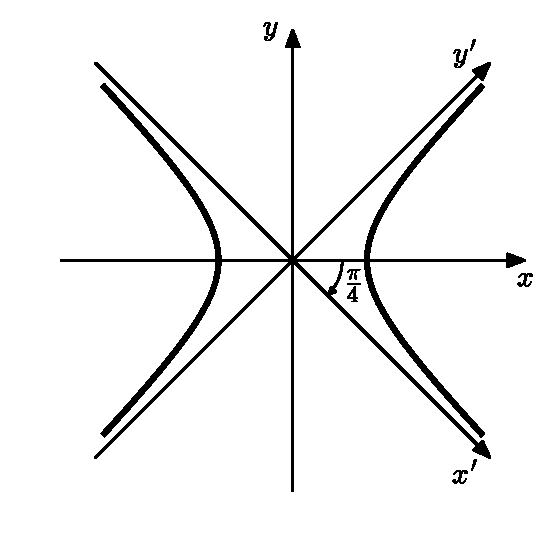
\includegraphics[width=\textwidth]{figuras/square_mapping_rotated_hyperbola.pdf}
  \end{minipage}\hfill
  \begin{minipage}[c]{0.45\textwidth}
    \caption{
       La rotación del eje de coordenadas \(xy\) de una hipérbola rectangular dada por la ecuación \ref{eq:hyperbola_canonical_equation} un ángulo de \(\pi/4\) radianes produce una hipérbola rectangular dada por la ecuación \ref{eq:rectangular_hyperbola_1st_3rd_quadrant_equation} contenida en el primer y tercer cuadrante en el nuevo eje de coordenadas \(x'y'\).
    } \label{fig:square_mapping_rotated_hyperbola}
  \end{minipage}
\end{figure}
Como se muestra en la figura \ref{fig:square_mapping_rotated_hyperbola}, esta es la ecuación de una hipérbola rectangular contenida en el primer y tercer cuadrante con 
\begin{itemize}
 \item eje mayor: la recta \(y=x\)
 \item centro: el origen de coordenadas
 \item vértices: \((\sqrt{a},\,\sqrt{a})\) y \((-\sqrt{a},\,-\sqrt{a})\)
 \item asíntotas: los ejes de coordenadas.
\end{itemize}

Retornando a la transformación \(w=z^2\) y teniendo en cuenta estas consideraciones, de la ecuación \ref{eq:square_mapping} se observa que cada rama de la hipérbola rectangular
\begin{equation}\label{eq:rectangular_hyperbola_horizontal}
 x^2-y^2=c_1\qquad\qquad\textrm{con}\qquad\qquad c_1>0,
\end{equation}
se mapea de forma uno a uno en la recta vertical \(u=c_1\). Efectivamente, la primera ecuación en \ref{eq:square_mapping} indica que \(u=c_1\) cuando \((x,\,y)\) es un punto de cualquier rama de la hipérbola. Además, los puntos con \(x=\sqrt{y^2+c_1}\) corresponden a la rama derecha y los puntos con \(x=-\sqrt{y^2+c_1}\) corresponden a la rama izquierda. Cuando por ejemplo un punto pertenece a la rama derecha, la segunda ecuación en \ref{eq:square_mapping} indica que \(v=2y\sqrt{y^2+c_1}\), y por lo tanto, la imagen de la rama derecha puede expresarse paramétricamente como
\[
 u=c_1,\qquad\qquad v=2y\sqrt{y^2+c_1}\qquad\qquad\textrm{con}\qquad\qquad-\infty<y<\infty.
\]
Esto muestra que la imagen de un punto \((x,\,y)\) en la rama derecha se mueve hacia arriba en la recta vertical a medida que \((x,\,y)\) se mueve hacia arriba en dicha rama. Análogamente, el par de ecuaciones
\[
 u=c_1,\qquad\qquad v=-2y\sqrt{y^2+c_1}\qquad\qquad\textrm{con}\qquad\qquad-\infty<y<\infty,
\]
es la representación paramétrica de la imagen de la rama izquierda de la hipérbola, y muestra que la imagen de un punto que se mueve hacia abajo por toda la rama izquierda es un punto que se mueve hacia arriba por toda la recta \(u=c_1\). Esto se ilustra en la figura \ref{fig:square_mapping_hyperbola}.
\begin{figure}[!htb]
 \begin{center}
 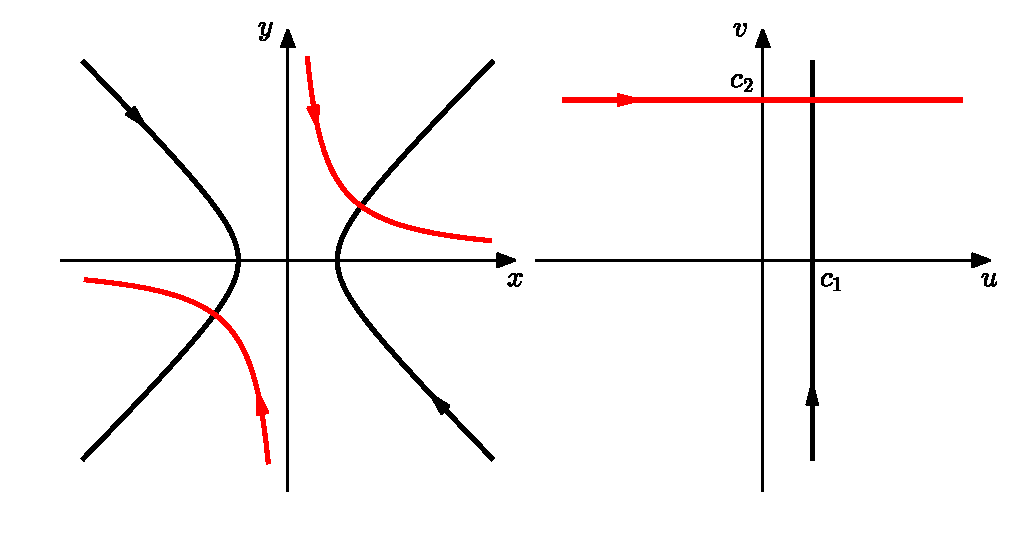
\includegraphics[width=0.85\textwidth]{figuras/square_mapping_hyperbola.pdf}
 \caption{\label{fig:square_mapping_hyperbola} Transformación \(w=z^2\). Las hipérbolas rectangulares \(x^2-y^2=c_1\) en el plano \(xy\) se mapean en rectas verticales \(u=c_1\) en el plano \(uv\) y las hipérbolas rectangulares \(2xy=c_2\) se mapean en rectas horizontales \(v=c_2\).}
 \end{center}
\end{figure}

Por otro lado, cada rama de la hipérbola 
\[
 2xy=c_2\qquad\qquad\textrm{con}\qquad\qquad c_2>0,
\]
se transforma en la recta \(v=c_2\). Para verificarlo, se observa de la segunda ecuación de \ref{eq:square_mapping} que \(v=c_2\) cuando \((x,\,y)\) es un punto de cualquiera de las ramas. Supóngase que el punto \((x,\,y)\) pertenece a la rama del primer cuadrante. Como \(y=c_2/(2x)\), la primera ecuación en \ref{eq:square_mapping} revela que la imagen de la rama tiene la representación paramétrica
\[
 u=x^2-\frac{c_2^2}{4x^2},\qquad\qquad v=c_2\qquad\qquad\textrm{con}\qquad\qquad0<x<\infty.
\]
Observando que 
\[
 \lim_{x\to0^+}u=-\infty
 \qquad\qquad\textrm{y}\qquad\qquad
 \lim_{x\to\infty}u=\infty,
\]
como \(u\) es continua en \(x\), es claro que a medida que \((x,\,y)\) se mueve hacia abajo en la rama del primer cuadrante, su imagen se mueve hacia la derecha sobre toda la recta \(v=c_2\). Además, la rama del tercer cuadrante tiene la representación paramétrica
\[
 u=\frac{c_2^2}{4y^2}-y^2,\qquad\qquad v=c_2\qquad\qquad\textrm{con}\qquad\qquad-\infty<y<0.
\]
Como
\[
 \lim_{y\to-\infty}u=-\infty
 \qquad\qquad\textrm{y}\qquad\qquad
 \lim_{y\to0^-}u=\infty,
\]
y \(u\) es continua en \(y\), se concluye que la imagen de un punto \((x,\,y)\) que se mueve hacia arriba en por toda la rama del tercer cuadrante se mueve hacia la derecha por toda la recta \(v=c_2\), como se muestra en la figura \ref{fig:square_mapping_hyperbola}.

\subsection*{Ejercicios}

A continuación se incluyen algunos ejercicios de la sección 14.

\subsubsection{Ejercicio 5}

Encontrar el dominio en el plano \(z\) cuya imagen bajo la transformación \(w=z^2\) es el dominio cuadrado en el plano \(w\) delimitado por las rectas \(u=1\), \(u=2\), \(v=1\) y \(v=2\).

\paragraph{Solución.} Según lo discutido en la sección \ref{sec:square_mapping}, el mapeo \(w=z^2\) transforma la hipérbola \(x^2-y^2=c\) del plano \(z\) en la recta vertical \(u=c\) del plano \(w\) y la hipérbola \(2xy=c\) del plano \(z\) en la recta horizontal \(v=c\) del plano \(w\), como se muestra en la figura \ref{fig:square_mapping_hyperbola}. Por lo tanto, el cuadrado del plano \(w\) es la imagen de la región delimitada por las hipérbolas
\[
 x^2-y^2=1,\qquad x^2-y^2=2, \qquad 2xy=1\qquad\textrm{y}\qquad 2xy=2, 
\]
que se muestra en la figura \ref{fig:exercise_14_05}. 
\begin{figure}[!htb]
 \begin{center}
 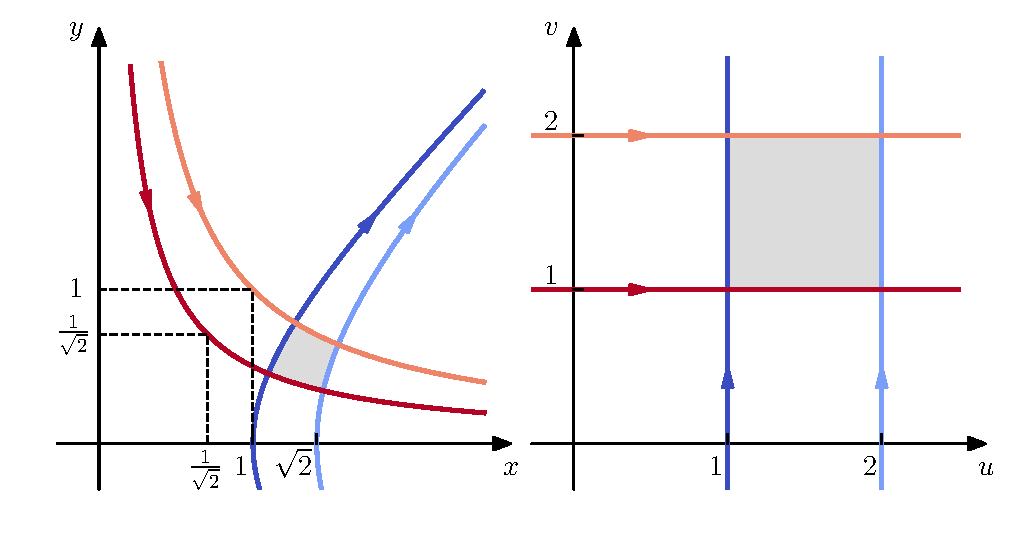
\includegraphics[width=0.85\textwidth]{figuras/exercise_14_05.pdf}
 \caption{\label{fig:exercise_14_05} Ejercicio 5. En la transformación \(w=z^2\) el cuadrado en el plano \(w\) es la imagen de la región delimitada por las hipérbolas en el plano \(z\).}
 \end{center}
\end{figure}

\subsubsection{Ejercicio 6}

Encontrar y graficar, mostrando las orientaciones correspondientes, las imágenes de las hipérbolas 
\[
 x^2-y^2=c_1,\qquad c_1<0\qquad\qquad\textrm{y}\qquad\qquad 2xy=c_2,\qquad c_2<0
\]
bajo la transformación \(w=z^2\).

\paragraph{Solución.} Se parte observando que
\[
 x^2-y^2=c_1,\qquad c_1<0
\]
es una hipérbola rectangular con eje mayor la recta \(x=0\) y vértices en \((0,\,\pm\sqrt{-c_1})\), como se muestra en la figura \ref{fig:exercise_14_06}. Esto es porque su ecuación se puede escribir como \(y^2-x^2=c_1'\) donde \(c_1'=-c_1>0\), por lo que su gráfica es como la hipérbola de la ecuación \ref{eq:rectangular_hyperbola_horizontal} pero intercambiando los ejes de coordenadas. La primera ecuación en \ref{eq:square_mapping} indica que cada rama de la hipérbola se transforma en la recta vertical \(u=c_1\). En particular, los puntos con \(y=\sqrt{x^2-c_1}\) corresponden a la rama superior y los puntos con \(y=-\sqrt{x^2-c_1}\) corresponden a la rama inferior. Cuando un punto pertenece a la rama superior, la segunda ecuación en \ref{eq:square_mapping} indica que \(v=2x\sqrt{x^2-c_1}\), y por lo tanto, la imagen de la rama superior puede expresarse paramétricamente como
\[
 u=c_1,\qquad\qquad v=2x\sqrt{x^2-c_1}\qquad\qquad\textrm{con}\qquad\qquad-\infty<x<\infty.
\]
Esto muestra que la imagen de un punto \((x,\,y)\) en la rama superior se mueve hacia arriba en la recta vertical a medida que \((x,\,y)\) se mueve hacia la derecha en dicha rama. Análogamente, la representación paramétrica de un punto en la rama inferior es
\[
 u=c_1,\qquad\qquad v=-2x\sqrt{x^2-c_1}\qquad\qquad\textrm{con}\qquad\qquad-\infty<x<\infty
\]
y muestra que a medida que \(x\) crece, \(v\) decrece. Por lo tanto, un punto \((x,\,y)\) en la rama inferior que se mueve a la izquierda tiene como imagen un punto que se mueve hacia arriba en la recta vertical \(u=c_1\). Esto se ilustra en la figura \ref{fig:exercise_14_06}.
\begin{figure}[!htb]
 \begin{center}
 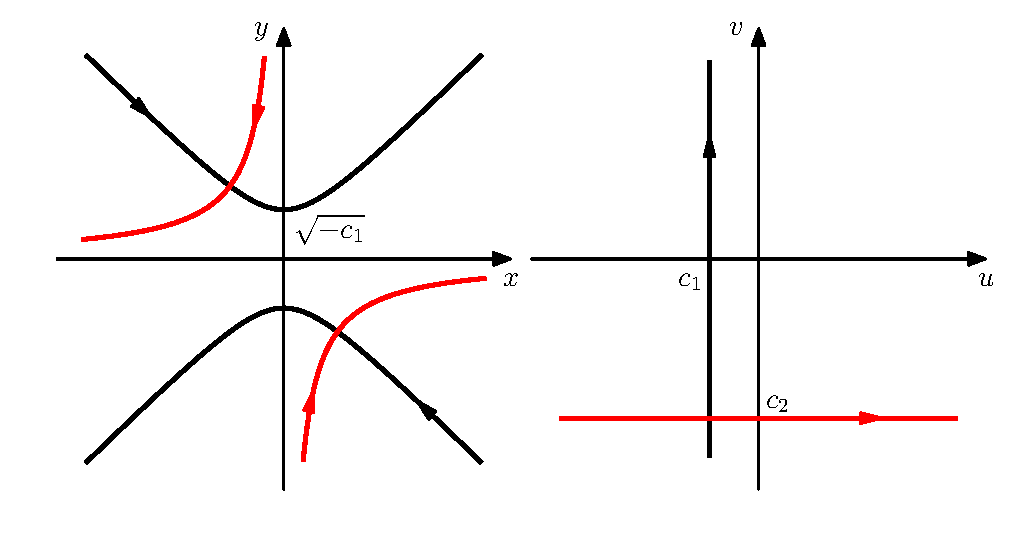
\includegraphics[width=0.85\textwidth]{figuras/exercise_14_06.pdf}
 \caption{\label{fig:exercise_14_06} Ejercicio 6. Imágenes de las hipérbolas rectangulares \(x^2-y^2=c_1\) con \(c_1<0\) y \(2xy=c_2\) con \(c_2<0\) bajo la transformación \(w=z^2\).}
 \end{center}
\end{figure}

Por otro lado, 
\[
 2xy=c_2,\qquad c_2<0
\]
es una hipérbola rectangular cuyas ramas están en el segundo y cuarto cuadrante, y la segunda ecuación en \ref{eq:square_mapping} indica que un punto en cualquier rama se transforma en un punto en la recta horizontal \(v=c_2\). La representación paramétrica de la rama del segundo cuadrante es
\[
 u=x^2-\frac{c_2^2}{4x^2},\qquad\qquad v=c_2\qquad\qquad\textrm{con}\qquad\qquad-\infty<x<0.
\]
Observando que 
\[
 \lim_{x\to-\infty}u=\infty
 \qquad\qquad\textrm{y}\qquad\qquad
 \lim_{x\to0^-}u=-\infty,
\]
como \(u\) es continua en \(x\), es claro que a medida que \((x,\,y)\) se mueve hacia abajo en la rama del segundo cuadrante, su imagen se mueve hacia la derecha sobre toda la recta \(v=c_2\). La representación paramétrica de la rama del cuarto cuadrante es
\[
 u=x^2-\frac{c_2^2}{4x^2},\qquad\qquad v=c_2\qquad\qquad\textrm{con}\qquad\qquad0<x<\infty,
\]
y como
\[
 \lim_{x\to0^+}u=-\infty
 \qquad\qquad\textrm{y}\qquad\qquad
 \lim_{x\to\infty}u=\infty,
\]
la imagen de un punto que se mueve hacia arriba en la rama del cuarto cuadrante es un punto que se mueve hacia la derecha en la recta \(v=c_2\), como se muestra en la figura \ref{fig:exercise_14_06}.

\subsubsection{Ejercicio 9}

Una interpretación de una función \(x=f(x,\,y)=u(x,\,y)+iv(x,\,y)\) es la de un \emph{campo vectorial} en el dominio de definición de \(f\). La función asigna un vector \(w\) con componentes \(u(x,\,y)\) y \(v(x,\,y)\) a cada punto \(z\) donde está definida. Indicar gráficamente los campos vectoriales representados por
\[
 (\textit{a})\;w=iz;\qquad\qquad (\textit{b})\;w=\frac{z}{|z|}.
\]
\paragraph{Solución}
\begin{enumerate}
 \item[(\textit{a})] Expresando \(z\) en coordenadas polares, \(z=re^{i\theta}\), y considerando que \(i=e^{i\pi/2}\), la transformación es
 \[
  w=iz=r\exp\left(\theta+\dfrac{\pi}{2}\right).
 \]
 Se observa que la transformación no altera el módulo y adiciona a la fase una magnitud de \(\pi/2\) radianes. Esto consiste en una rotación de \(\pi/2\) radianes en sentido antihorario del vector \(z\). El campo vectorial asociado a la transformación se muestra en la figura \ref{fig:exercise_14_09}.
 \item[(\textit{b})] La transformación \(w=z/|z|\) no altera la fase por tratarse únicamente de la división del vector \(z\) entre un número real y es tal que \(|w|=1\) para todo \(z\neq0\). El campo vectorial se muestra en la figura \ref{fig:exercise_14_09}.
\end{enumerate}
\begin{figure}[!htb]
 \begin{center}
 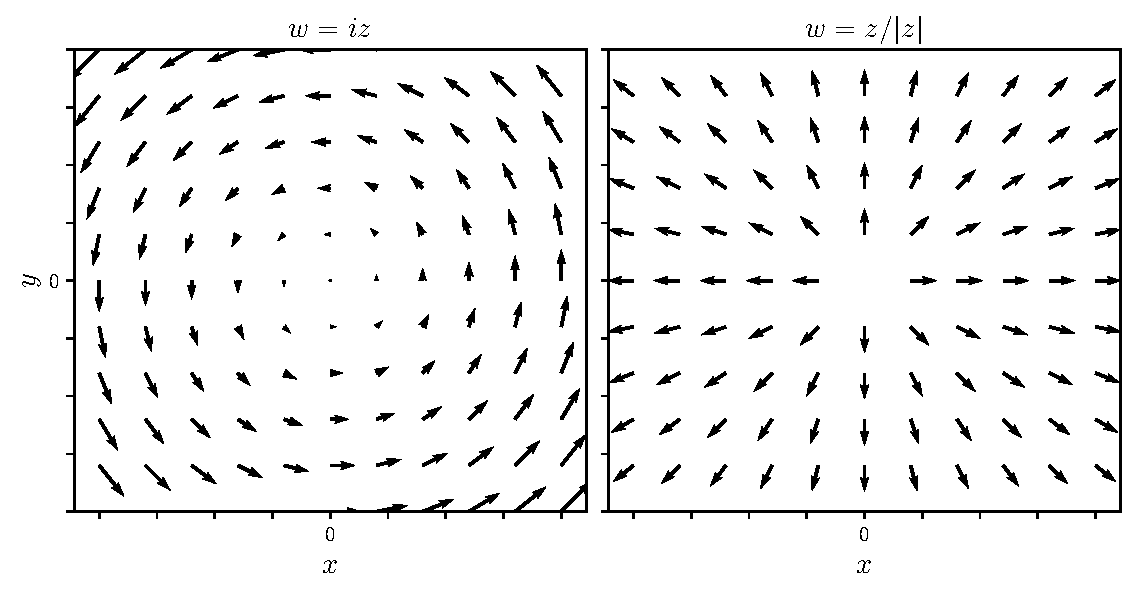
\includegraphics[width=0.9\textwidth]{figuras/exercise_14_09.pdf}
 \caption{\label{fig:exercise_14_09} Ejercicio 9. Campos vectoriales asociados a las transformaciones \(w=iz\) y \(w=z/|z|\).}
 \end{center}
\end{figure}

\section{Límites}

Sea una función \(f\) definida en todos los puntos \(z\) de un entorno reducido de un punto \(z_0\). La afirmación de que \(f(z)\) tiene límite \(w_0\) cuando \(z\) se aproxima a \(z_0\), o
\begin{equation}\label{eq:limit_statement}
 \lim_{z\to z_0}f(z)=w_0, 
\end{equation}
significa que el punto \(w=f(z)\) puede hacerse arbitrariamente cercano a \(w_0\) si se elige el punto \(z\) suficientemente cercano a \(z_0\) pero distinto de él. A continuación se expresa la definición formal.

La afirmación de la ecuación \ref{eq:limit_statement} significa que para cada número positivo \(\epsilon\), existe un número positivo \(\delta\) tal que
\begin{equation}\label{eq:limit_definition}
 |f(z)-w_0|<\epsilon\qquad\textrm{para todo }z\textrm{ tal que}\qquad0<|z-z_0|<\delta. 
\end{equation}
Geométricamente, la definición indica que para cada entorno de \(w_0\) de radio \(\epsilon\), \(|w-w_0|<\epsilon\), existe un entorno reducido de \(z_0\) de radio \(\delta\), \(0<|z-z_0|<\delta\), tal que cada punto \(z\) en él tiene su imagen \(w\) en el entorno de radio \(\epsilon\) de \(w_0\). Observar que si bien todos los puntos del entorno reducido \(0<|z-z_0|<\delta\) deben ser considerados, sus imágenes no tienen porque abarcar el entorno \(|w_0-w|<\epsilon\) completo. Notar además que una vez que se encontró un valor de \(\delta\) que cumpla la condición, puede ser sustituido por cualquier número positivo menor, como \(\delta/2\) por ejemplo.

\paragraph{Teorema: unicidad del límite.} Cuando el límite de una función \(f(z)\) existe en el punto \(z_0\), es único.\\[1ex]

La definición \ref{eq:limit_definition} requiere que \(f\) esté definida en todos los puntos del entorno reducido de \(z_0\). Dicho entorno reducido siempre existe si \(z_0\) es un punto interior de la región en donde \(f\) está definida. La definición de límite puede extenderse al caso en que \(z_0\) es un punto de la frontera de la región de definición de \(f\) acordando que la primera inecuación en \ref{eq:limit_definition} debe satisfacerse únicamente para los puntos \(z\) que pertenecen a intersección de la región de definición de \(f\) con entorno reducido.  

Si el limite \ref{eq:limit_statement} existe, la notación \(z\to z_0\) implica que \(z\) se aproxima a \(z_0\) de forma arbitraria y no en una dirección en particular. 

\section{Teoremas sobre límites}\label{sec:limits_theorems}

El estudio sobre límites puede abreviarse estableciendo una conexión entre el límite de funciones de variable compleja y el límite de funciones reales de dos variables reales. Como los límites del último tipo se estudian en cálculo, sus definiciones y propiedades pueden emplearse libremente. 

\paragraph{Teorema 1.} Supóngase que 
\[
 f(z)=u(x,\,y)+iv(x,\,y),\qquad\qquad\textrm{con}\qquad\qquad z=x+iy,
\]
y
\[
 z_0=x_0+iy_0,\qquad\qquad w_0=u_0+iv_0.
\]
Si
\[
 \lim_{(x,\,y)\to(x_0,\,y_0)}u(x,\,y)=u_0
 \qquad\qquad\textrm{y}\qquad\qquad
 \lim_{(x,\,y)\to(x_0,\,y_0)}v(x,\,y)=v_0
\]
se cumple que 
\[
 \lim_{z\to z_0}f(z)=w_0.
\]
Lo recíproco también es cierto.

\paragraph{Teorema 2.} Supóngase que
\[
 \lim_{z\to z_0}f(z)=w_0
 \qquad\qquad\textrm{y}\qquad\qquad
 \lim_{z\to z_0}F(z)=W_0.
\]
Entonces, se cumple que 
\begin{equation}\label{eq:limits_functions_operations}
 \lim_{z\to z_0}[f(z)+F(z)]=w_0+W_0,
 \qquad
 \lim_{z\to z_0}f(z)F(z)=w_0W_0
 \qquad\textrm{y}\qquad 
 \lim_{z\to z_0}\frac{f(z)}{F(z)}=\frac{w_0}{W_0},
\end{equation}
donde en el último límite se debe imponer la condición adicional de que \(W_0\neq0\).

\section{Límites que involucran el punto en el infinito}\label{sec:limits_infinity_point}

En ocasiones es conveniente incluir en el plano complejo el \emph{punto en el infinito}, denotado como \(\infty\), y emplear límites que lo involucran. El plano complejo en conjunto con este punto se denomina \emph{plano complejo extendido}. Para visualizar el punto en el infinito, se puede pensar en el plano complejo como pasando por el ecuador de una esfera unidad centrada en el origen, como se muestra en la figura \ref{fig:point_at_infinity_mayavi_v2_resize}. A cada punto \(z\) en el plano complejo le corresponde exactamente un punto \(P\) en la superficie de la esfera. El punto \(P\) es el punto donde la recta que pasa por \(z\) y el polo norte \(N\) intersecta la esfera. De forma similar, a cada punto \(P\) de la esfera, excepto al polo norte \(N\), le corresponde exactamente un punto \(z\)  en el plano complejo. Si se asigna al polo norte \(N\) de la esfera el punto en el infinito, se obtiene una correspondencia uno a uno entre puntos de la esfera y puntos del plano complejo extendido. La esfera se conoce como \emph{esfera de Riemann} y la correspondencia se llama \emph{proyección estereográfica}.
\begin{figure}[!htb]
 \begin{center}
 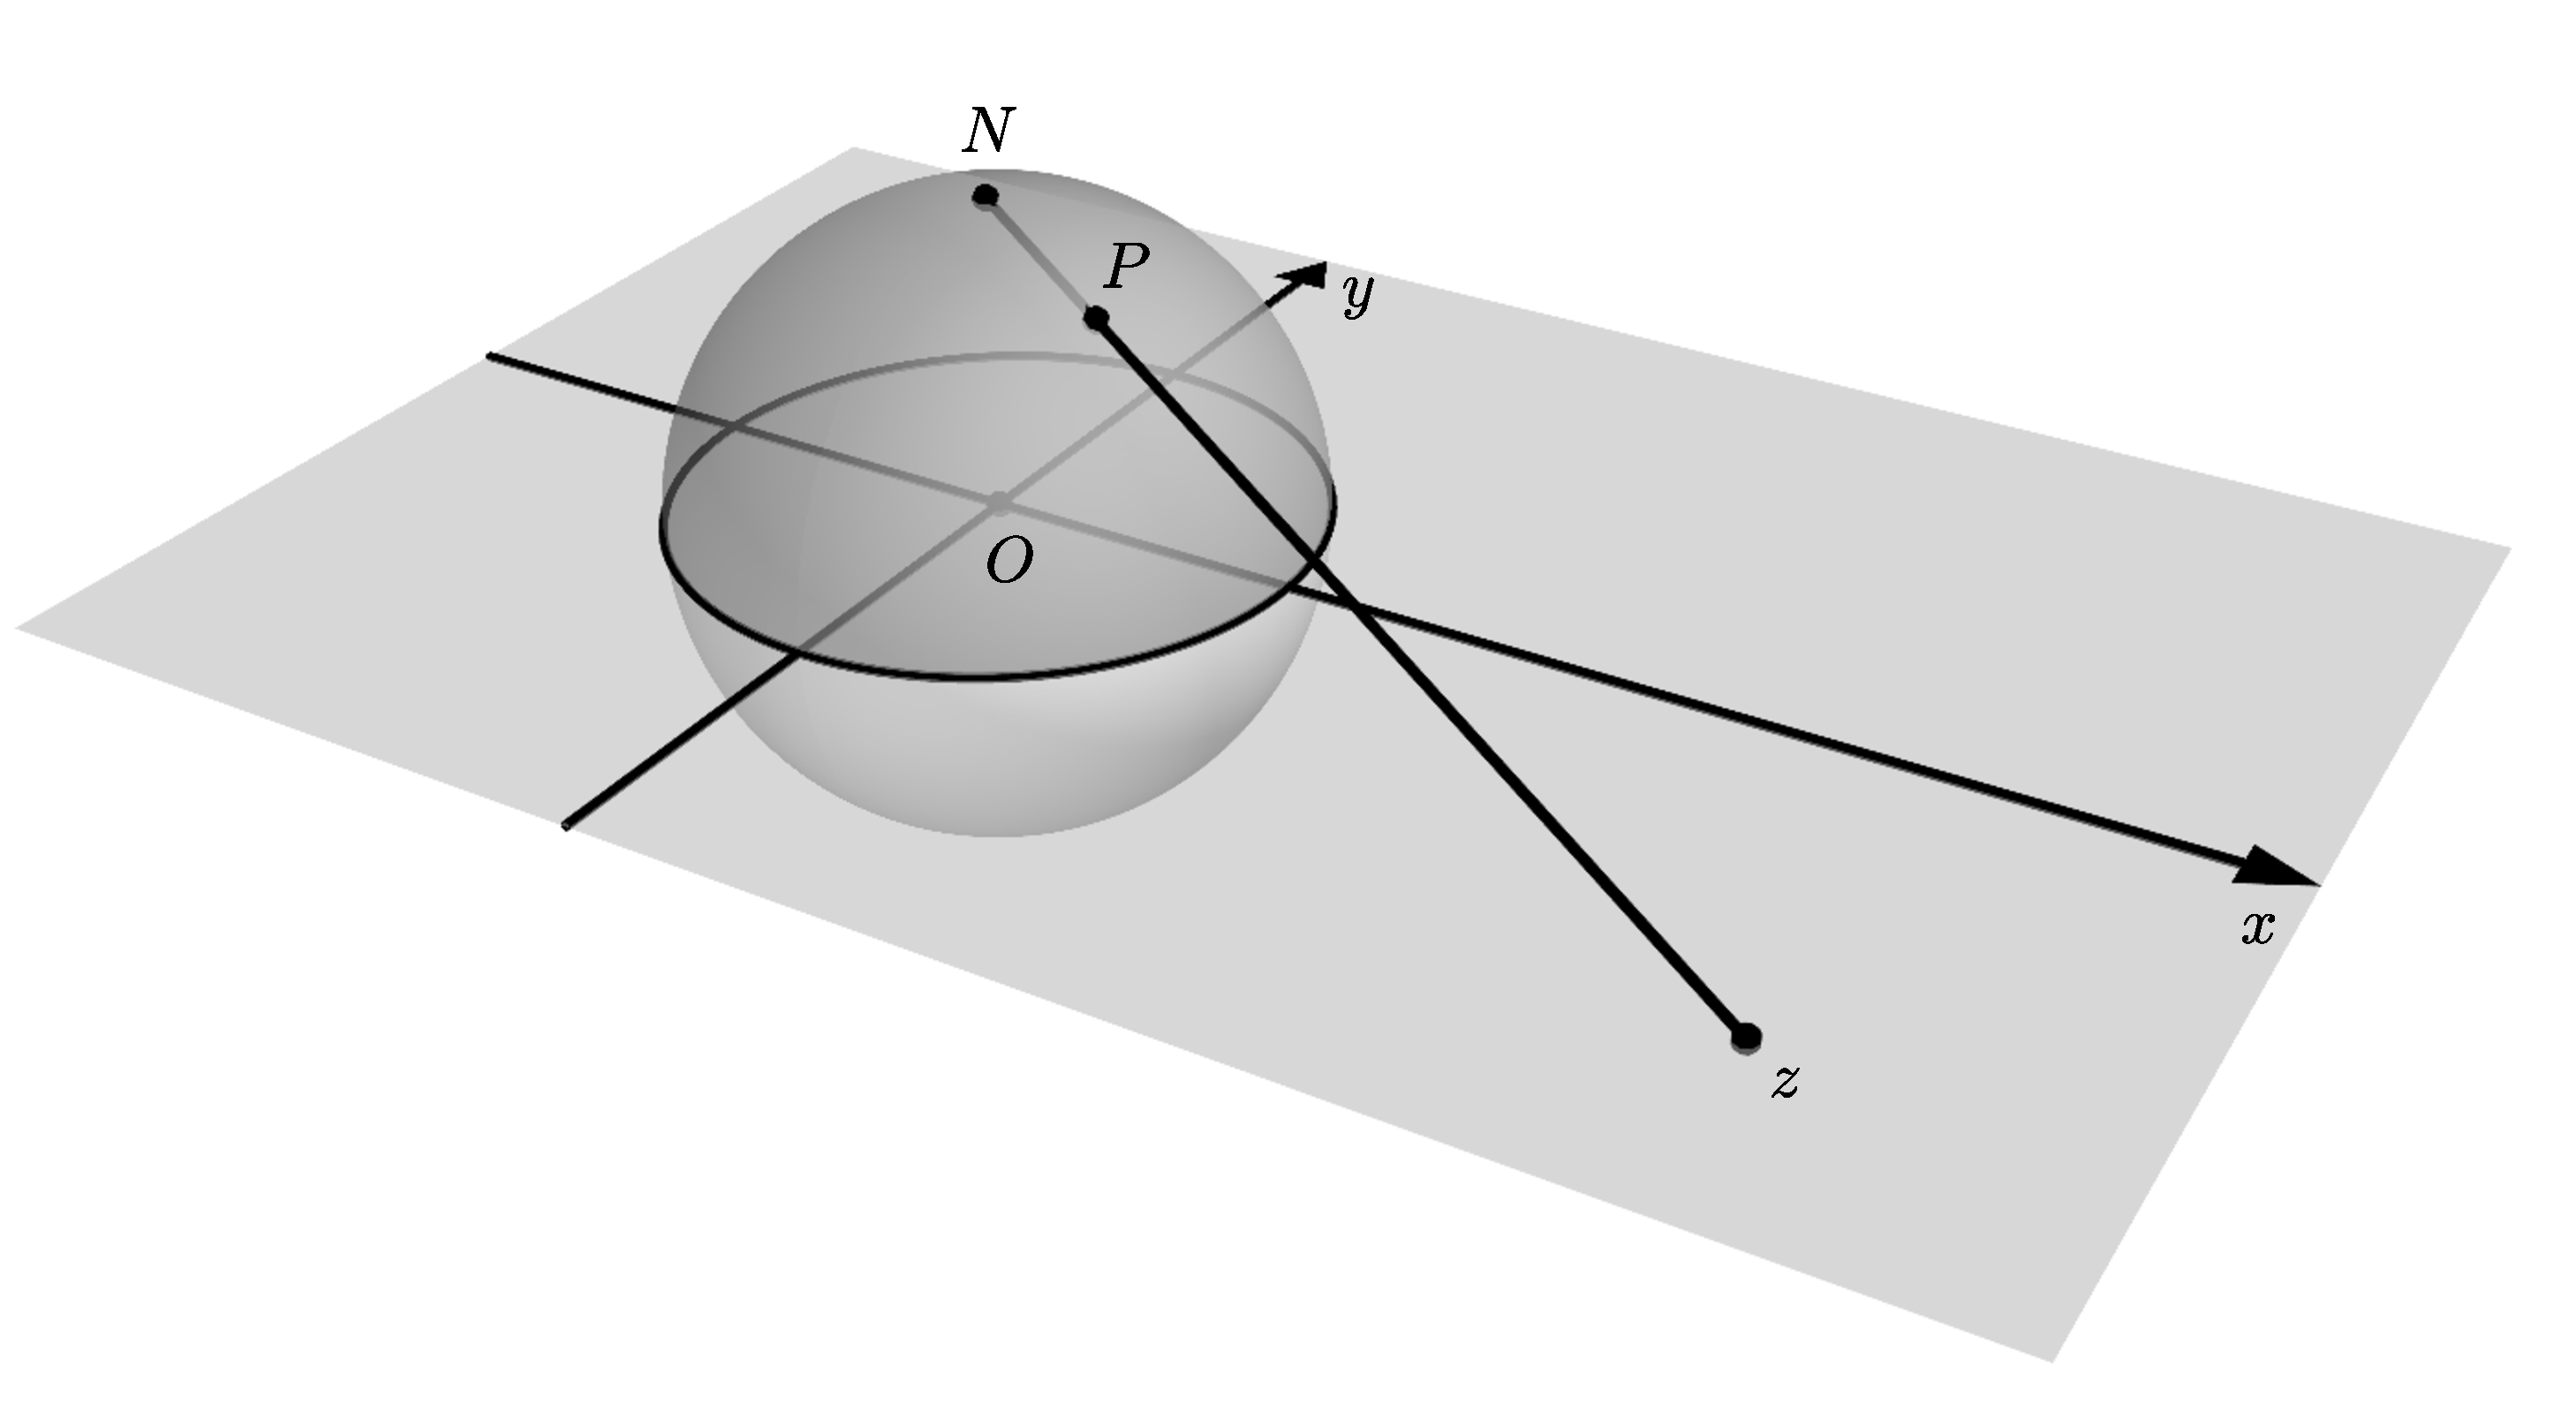
\includegraphics[width=0.95\textwidth]{figuras/point_at_infinity_mayavi_v2_resize.pdf}
 \caption{\label{fig:point_at_infinity_mayavi_v2_resize} Proyección estereográfica.}
 \end{center}
\end{figure}


Observar que el exterior del círculo unidad centrado en el origen en el plano complejo, corresponde al hemisferio norte con el ecuador y el polo norte \(N\) omitidos. Además, para cada número pequeño positivo \(\epsilon\), los puntos en el plano complejo exteriores a la circunferencia \(|z|=1/\epsilon\) corresponden a puntos en la esfera cercanos a \(N\). Por lo tanto, al conjunto \(|z|>1/\epsilon\) se le llama \emph{entorno de }\(\infty\).

Como convención, al referirse a un punto \(z\), se asumirá que se trata de un punto del \emph{plano finito}. Por lo tanto, cuando haya que referirse al punto en el infinito, se hará explícitamente.

Teniendo en cuenta estas consideraciones, ya es posible darle un significado a la afirmación
\[
 \lim_{z\to z_0} f(z)=w_0
\]
cuando \(z_0\) o \(w_0\), o posiblemente ambos números, son reemplazados por el punto en el infinito. Para hacerlo, en la definición del límite dada por la ecuación \ref{eq:limit_definition} simplemente se reemplaza el entorno correspondiente de \(z_0\) o \(w_0\) por un entorno de \(\infty\). La prueba del siguiente teorema ilustra como se hace.

\paragraph{Teorema.} Si \(z_0\) y \(w_0\) son puntos en el pano \(z\) y \(w\) respectivamente, entonces,
\[
 \lim_{z\to z_0} f(z)=\infty
  \qquad\qquad\textrm{si}\qquad\qquad
 \lim_{z\to z_0} \frac{1}{f(z)}=0 
\]
y
\[
 \lim_{z\to \infty} f(z)=w_0
  \qquad\qquad\textrm{si}\qquad\qquad
 \lim_{z\to 0}f\left(\frac{1}{z}\right)=w_0. 
\]
Además,
\[
 \lim_{z\to \infty} f(z)=\infty
  \qquad\qquad\textrm{si}\qquad\qquad
 \lim_{z\to 0}\frac{1}{f(1/z)}=0. 
\]
Se incluye a continuación la prueba solo de la primera afirmación. Asumiendo que se cumple el segundo límite en la primera afirmación, la definición de límite \ref{eq:limit_definition} indica que para todo número \(\epsilon\) positivo, existe un número \(\delta\) positivo tal que 
\[
 \left|\frac{1}{f(z)}-0\right|<\epsilon
 \qquad\textrm{si se cumple que}\qquad
 0<|z-z_0|<\delta.
\]
Como esto puede escribirse como
\[
 |f(z)|>\frac{1}{\epsilon}
 \qquad\textrm{si se cumple que}\qquad
 0<|z-z_0|<\delta,
\]
se obtiene el primer límite de la primera afirmación, ya que la expresión indica que \(f(z)\) se encuentra en un entorno de \(\infty\).

\section{Continuidad}\label{sec:continuity_definition}

Una función \(f\) es \emph{continua} en el punto \(z_0\) si se cumplen las siguientes tres condiciones:
\begin{enumerate}
 \item \(\displaystyle\lim_{z\to z_0}f(z)\) existe.
 \item \(\displaystyle f(z_0)\) existe.
 \item \(\displaystyle\lim_{z\to z_0}f(z)=f(z_0)\).
\end{enumerate}
Observar que la afirmación 3. contiene las afirmaciones 1. y 2., ya que la existencia de los valores en ambos lados de la igualdad de la ecuación es necesaria. La afirmación 3. indica que para todo número \(\epsilon\) positivo existe un número \(\delta\) positivo tal que
\begin{equation}\label{eq:continuity_definition}
 |f(z)-f(z_0)|<\epsilon
 \qquad\textrm{si se cumple que}\qquad
 |z-z_0|<\delta.
\end{equation}

Una función de variable compleja se dice continua en una región \(R\) si es continua en cada punto de \(R\).

Si dos funciones son continuas en un punto, su suma y su producto también son continuas en ese punto, y su cociente es una función continua si el denominador no es cero en ese punto. Esto es consecuencia de la ecuación \ref{eq:limits_functions_operations}.

A continuación se incluyen otras propiedades de funciones continuas como teoremas, cuya verificación no es tan inmediata.

\paragraph{Teorema 1.} La composición de funciones continuas es una función continua. 

Sea \(w=f(z)\) una función definida para todo \(z\) en el entorno \(|z-z_0|<\delta\) del punto \(z_0\), y sea \(W=g(w)\) una función cuyo dominio de definición contiene la imagen de dicho entorno bajo \(f\). De esta forma, la composición \(W=g[f(z)]\) está definida para todo el entorno \(|z-z_0|<\delta\). Si \(f\) es continua en \(z_0\) y \(g\) es continua en el punto \(f(z_0)\) del plano \(w\), se cumple que \(g[f(z)]\) es continua en \(z_0\).

\paragraph{Teorema 2.} Si una función \(f(z)\) es continua y no nula en el punto \(z_0\), entonces \(f(z)\neq0\) en algún entorno de ese punto.

\paragraph{Teorema 3.} Sea
\[
 f(z)=u(x,\,y)+iv(x,\,y).
\]
Si las funciones componentes \(u\) y \(v\) son continuas en el punto \(z_0=(x_0,\,y_0)\), también los es \(f\). Recíprocamente, si \(f\) es continua en el punto \(z_0\), también los son \(u\) y \(v\) en ese punto.

\paragraph{Teorema 4.} Si una función \(f\) es continua en una región \(R\) cerrada y acotada, existe un número \(M\) no negativo tal que 
\[
 |f(z)|\leq M\qquad\textrm{para todos los puntos }z\textrm{ en }R,
\]
y la igualdad se cumple para al menos un punto \(z\) de \(R\). En estas condiciones, se dice que \(f\) es \emph{acotada en }\(R\).

\subsection*{Ejercicios}

\subsubsection{Ejercicio 1}

Emplear la definición de límite dada por la ecuación \ref{eq:limit_definition} para probar que 
\[
 (\textit{a})\;\lim_{z\to z_0}\Re z=\Re z_0;\qquad\qquad 
 (\textit{b})\;\lim_{z\to z_0}\overline{z}=\overline{z_0};\qquad\qquad
 (\textit{c})\;\lim_{z\to z_0}\frac{\overline{z}^2}{z}=0.
\]

\paragraph{Solución.} 
\begin{enumerate}
 \item[(\textit{a})] Hay que probar que para todo número \(\epsilon\) positivo, existe un número \(\delta\) positivo tal que 
\begin{equation}\label{eq:exersice_18_01_a_limit}
 |\Re z-\Re z_0|<\epsilon
 \qquad\textrm{si se cumple que}\qquad
 0<|z-z_0|<\delta.
\end{equation}
Sea \(z=x+iy\) y \(z_0=x_0+iy_0\). De esta forma,
\[
 |\Re z-\Re z_0|=|x-x_0|.
\]
Por otro lado,
\[
 |z-z_0|=|(x+iy)-(x_0+iy_0)|=|(x-x_0)+i(y-y_0)|\geq|x-x_0|
\]
Combinando los resultados, se tiene que 
\[
 |\Re z-\Re z_0|=|x-x_0|\leq|z-z_0|.
\]
Por lo tanto, eligiendo \(\delta=\epsilon\) se cumple \ref{eq:exersice_18_01_a_limit} para todo \(\epsilon>0\).
\item[(\textit{b})] Hay que probar que para todo \(\epsilon>0\), existe \(\delta\) tal que
\begin{equation}\label{eq:exersice_18_01_b_limit}
 |\overline{z}-\overline{z_0}|<\epsilon
 \qquad\textrm{si se cumple que}\qquad
 0<|z-z_0|<\delta.
\end{equation}
Como 
\[
 |\overline{z}-\overline{z_0}|=|\overline{(z-z_0)}|=|z-z_0|,
\]
eligiendo \(\delta=\epsilon\), se cumple la ecuación \ref{eq:exersice_18_01_b_limit} para todo \(\epsilon>0\).
\item[(\textit{c})] Hay que probar que para todo \(\epsilon>0\), existe \(\delta\) tal que
\begin{equation}\label{eq:exersice_18_01_c_limit}
 \left|\frac{\overline{z}^2}{z}-0\right|<\epsilon
 \qquad\textrm{si se cumple que}\qquad
 0<|z-0|<\delta.
\end{equation}
Observando que 
\[
 \left|\frac{\overline{z}^2}{z}-0\right|=\left|\frac{\overline{z}^2}{z}\right|=\frac{|\overline{z}|^2}{|z|}=\frac{|z|^2}{|z|}=|z|,
\]
eligiendo \(\delta=\epsilon\), se cumple la ecuación \ref{eq:exersice_18_01_c_limit} para todo \(\epsilon>0\).
\end{enumerate}

\subsubsection{Ejercicio 2}

Sean las constantes complejas \(a\), \(b\) y \(c\). Emplear la definición de límite dada por la ecuación \ref{eq:limit_definition} para probar que 
\begin{align*}
 (\textit{a})\;&\lim_{z\to z_0}(az+b)=az_0+b;\qquad\qquad\qquad
 (\textit{b})\;\lim_{z\to z_0}(z^2+c)=z_0^2+c;\\
 (\textit{c})\;&\lim_{z\to1-i}x+i(2x+y)=1+i,\qquad\textrm{con}\qquad z=x+iy.
\end{align*}

\paragraph{Solución.} 
\begin{enumerate}
 \item[(\textit{a})] Sea \(\epsilon>0\) y supóngase que \(|z-z_0|<\delta\). Si \(a=0\), se cumple que 
 \[
  |(az+b)-(az_0+b)|=|b-b|=0<\epsilon.
 \]
 Si \(a\neq0\),
 \[
  |(az+b)-(az_0+b)|=|a||z-z_0|<|a|\delta.
 \]
 Por lo tanto, eligiendo \(\delta=\epsilon/|a|\), se cumple que 
 \[
  |(az+b)-(az_0+b)|<\epsilon
  \qquad\textrm{si se cumple que}\qquad
  0<|z-z_0|<\delta=\frac{\epsilon}{|a|}.
 \]
 \item[(\textit{b})] Sea \(\epsilon>0\) y supóngase que \(|z-z_0|<\delta\). Se observa que
 \begin{align*}
  |(z^2+c)-(z_0^2+c)|&=|z^2-z_0^2|\\
   &=|z+z_0||z-z_0|\\
   &=|z-z_0+2z_0||z-z_0|\\
   &\leq(|z-z_0|+2|z_0|)|z-z_0|\\
   &<(\delta+2|z_0|)\delta.
 \end{align*}
 Por lo tanto, eligiendo \(\delta\) tal que \((\delta+2|z_0|)\delta=\epsilon\), es decir, \(\delta=\sqrt{|z_0|^2+\epsilon}-|z_0|\), se cumple que 
 \[
  |(z^2+c)-(z_0^2+c)|<\epsilon
  \qquad\textrm{si se cumple que}\qquad
  0<|z-z_0|<\delta.
 \]
 
 A continuación se resolverá el problema de forma alternativa para obtener un resultado mas simple. El método es clásico en las pruebas \emph{epsilon-delta}. Se parte igual que antes planteando la condición \(|f(z)-w_0|<\epsilon\), que en este caso es
 \begin{equation}\label{eq:exersice_18_02_b_epsilon_condition}
  |(z^2+c)-(z_0^2+c)|=|z^2-z_0^2|=|z+z_0||z-z_0|<\epsilon,
 \end{equation}
 y al despejar el término \(|z-z_0|\), la condición queda
 \begin{equation}\label{eq:exersice_18_02_b_delta_condition}
  |z-z_0|<\frac{\epsilon}{|z+z_0|}.
 \end{equation}
 De esta forma, podría establecerse \(\delta=\epsilon/|z+z_0|\), pero \(\delta\) debe depender solo de \(\epsilon\) y no de otras variables, por lo que hay que eliminar el factor \(|z+z_0|\). Para hacerlo, se considera que el concepto de límite se aplica solo cuando \(z\) es suficientemente cercano a \(z_0\), por lo que se restringirá al caso en que \(z\) diste a los sumo 1 de \(z_0\), es decir, \(|z-z_0|<1\). Así, el término \(|z+z_0|\) cumple que
 \[
  |z+z_0|=|z-z_0+2z_0|\leq|z-z_0|+2|z_0|<1+2|z_0|,
 \]
 donde la última desigualdad proviene de la condición \(|z-z_0|<1\). Se obtuvo que
 \begin{equation}\label{eq:exersice_18_02_b_z_condition}
  |z+z_0|<1+2|z_0|.
 \end{equation}
 Ahora, el lado derecho de la ecuación \ref{eq:exersice_18_02_b_delta_condition} es mínimo cuando de denominador es máximo, por lo que sustituyendo el resultado de la ecuación \ref{eq:exersice_18_02_b_z_condition} resulta en
 \[
  |z-z_0|<\frac{\epsilon}{1+2|z_0|}.
 \]
 Como se tienen las dos condiciones
 \[
  |z-z_0|<1
   \qquad\qquad\textrm{y}\qquad\qquad
  |z-z_0|<\frac{\epsilon}{1+2|z_0|},
 \]
 se elige
 \[
  \delta=\min\left\{1,\,\frac{\epsilon}{1+2|z_0|}\right\}.
 \]
 Finalmente, se verificará que con esta elección de \(\delta\), se satisface la condición \ref{eq:exersice_18_02_b_epsilon_condition}.
 \begin{itemize}
  \item Se considera el caso en que \(\delta=1\) y por lo tanto
  \[
   1<\frac{\epsilon}{1+2|z_0|},
   \qquad\qquad\textrm{es decir}\qquad\qquad 1+2|z_0|<\epsilon.
  \]
  La condición \(|z-z_0|<\delta\) es en este caso \(|z-z_0|<1\), por lo que multiplicando por \(|z+z_0|\) a ambos lados de la inecuación, se tiene que 
  \[
   |z-z_0||z+z_0|<|z+z_0|\overset{(a)}{<}1+2|z_0|<\epsilon,
  \]
  donde en \((a)\) se empleó la ecuación \ref{eq:exersice_18_02_b_z_condition}. Esto indica que se cumple que \(|f(z)-w_0|<\epsilon\) si \(|z-z_0|<\delta\), como se requiere.
  \item Sea ahora
  \[
   \delta=\frac{\epsilon}{1+2|z_0|}.
  \]
  La condición \(|z-z_0|<\delta\) es en este caso
  \[
   |z-z_0|<\frac{\epsilon}{1+2|z_0|},
  \]
  y al multiplicar por \(|z+z_0|\) a ambos lados de la inecuación se obtiene que 
  \[
   |z-z_0||z+z_0|<\frac{\epsilon}{1+2|z_0|}|z+z_0|\overset{(a)}{<}\frac{\epsilon}{1+2|z_0|}(1+2|z_0|)=\epsilon,
  \]
  donde en \((a)\) se empleó la ecuación \ref{eq:exersice_18_02_b_z_condition}.
 \end{itemize} 
 \item[(\textit{c})] Sea \(z=x+iy\). Hay que probar que para todo \(\epsilon>0\), existe \(\delta>0\) tal que
 \begin{equation}\label{eq:exersice_18_02_c_limit}
  |[x+i(2x+y)]-(1+i)|<\epsilon
  \qquad\textrm{si se cumple que}\qquad
  0<|(x+iy)-(1-i)|<\delta.
 \end{equation}
 Por un lado se tiene que 
 \[
  |(x+iy)-(1-i)|=|(x-1)+i(y-1)|,
 \]
 y por lo tanto, asumiendo que
 \begin{equation}\label{eq:exersice_18_02_c_delta_condition}
  |(x+iy)-(1-i)|<\delta
  \qquad\textrm{se cumple que}\qquad
  |x-1|<\delta\qquad\textrm{y}\qquad|y+1|<\delta.
 \end{equation}
 Por otro lado, se observa que 
 \begin{align*}
  |[x+i(2x+y)]-(1+i)|&=|(x-1)+i(2x+y-1)|\\
   &\leq|x-1|+|2x+y-1|\\
   &=|x-1|+|2x-2+y+1|\\
   &\leq|x-1|+2|x-1|+|y+1|\\
   &\overset{(a)}{<}\delta+2\delta+\delta\\
   &=4\delta,
 \end{align*}
 donde en \((a)\) se asumió que se cumple la condición de la ecuación \ref{eq:exersice_18_02_c_delta_condition}. Por lo tanto, eligiendo \(\delta=\epsilon/4\), se cumple \ref{eq:exersice_18_02_c_limit}.
\end{enumerate}

\subsubsection{Ejercicio 3}

Sea \(n\) un entero positivo y sean \(P(z)\) y \(Q(z)\) polinomios, con \(Q(z_0)\neq0\). Emplear los resultados del teorema que conduce a la ecuación \ref{eq:limits_functions_operations} para encontrar
\[
 (\textit{a})\;\lim_{z\to z_0}\frac{1}{z^n};\qquad\qquad 
 (\textit{b})\;\lim_{z\to i}\frac{iz^3-1}{z+i};\qquad\qquad
 (\textit{c})\;\lim_{z\to z_0}\frac{P(z)}{Q(z)}.
\]

\paragraph{Solución.} 

\begin{enumerate}
 \item[(\textit{a})] 
 \(\displaystyle\lim_{z\to z_0}\frac{1}{z^n}=\frac{1}{\lim\limits_{z\to z_0}z^n}=\frac{1}{z_0^n}\)
 \item[(\textit{b})] 
 \(\displaystyle\lim_{z\to i}\frac{iz^3-1}{z+i}=\frac{\lim\limits_{z\to i}iz^3-1}{\lim\limits_{z\to i}z+i}=\frac{i(i^3)-1}{i+i}=\frac{1-1}{2i}=0\).
 \item[(\textit{c})]
 \(\displaystyle\lim_{z\to z_0}\frac{P(z)}{Q(z)}=\frac{\lim\limits_{z\to z_0}P(z)}{\lim\limits_{z\to z_0}Q(z)}=\frac{P(z_0)}{Q(z_0)}\).
\end{enumerate}

\subsubsection{Ejercicio 4}

Emplear inducción matemática y el resultado de la ecuación \ref{eq:limits_functions_operations} para mostrar que
\begin{equation}\label{eq:exersice_18_04_objective}
 \lim_{z\to z_0}z^n=z_0^n,
\end{equation}
donde \(n\) es un entero positivo.

\paragraph{Solución.} Se considera primero el \emph{caso base} en que \(n=1\). Consiste en probar que 
\[
 \lim_{z-z_0}z=z_0,
\]
lo que es directo: es fácil ver que alcanza con elegir \(\delta=\epsilon\) en la definición de límite dada por la ecuación \ref{eq:limit_definition}. El \emph{paso inductivo} consiste en mostrar que si la ecuación \ref{eq:exersice_18_04_objective} se cumple para \(n=k\), se cumple para \(n=k+1\), es decir,
\[
 \lim_{z\to z_0}z^k=z_0^k
 \qquad\qquad\Rightarrow\qquad\qquad
 \lim_{z\to z_0}z^{k+1}=z_0^{k+1}.
\] 
Como
\[
 \lim_{z\to z_0}z^{k+1}=\lim_{z\to z_0}z^kz\overset{(a)}{=}\left(\lim_{z\to z_0}z^k\right)\left(\lim_{z\to z_0}z\right)\overset{(b)}{=}z_0^kz_0=z_0^{k+1},
\]
donde en \((a)\) se empleó el resultado de la ecuación \ref{eq:limit_definition} y en \((b)\) se empleó el caso base y la hipótesis de inducción, concluyendo la prueba.

\subsubsection{Ejercicio 5}

Mostrar que la función
\[
 f(z)=\left(\frac{z}{\overline{z}}\right)^2
\]
tiene valor 1 en todos los puntos no nulos de los ejes real e imaginario, donde \(z=(x,\,0)\) y \(z=(0,\,y)\) respectivamente, pero tiene valor \(-1\) en todos los puntos no nulos de la recta \(y=x\), donde \(z=(x,\,x)\). Esto muestra que el límite de \(f(z)\) cuando \(z\) tiende a 0 no existe. Observar que no es suficiente considerar únicamente los puntos no nulos \(z=(x,\,0)\) y \(z=(0,\,y)\) por ejemplo.

\paragraph{Solución.} Con \(z=x+iy\),
\[
 f(z)=\left(\frac{z}{\overline{z}}\right)^2=\left(\frac{x+iy}{x-iy}\right)^2.
\]
En el caso en que \(z=(x,\,0)\), se tiene que 
\[
 f(z)=\left(\frac{x+i0}{x-i0}\right)^2=1.
\]
En el caso en que \(z=(0,\,y)\), se cumple que 
\[
 f(z)=\left(\frac{0+iy}{0-iy}\right)^2=1.
\]
Pero si \(z=(x,\,x)\),
\[
 f(z)=\left(\frac{x+ix}{x-ix}\right)^2=\frac{x^2-x^2+2ix^2}{x^2-x^2-2ix^2}=-1.
\]
Como \(f(z)\) tiene valor 1 en todos los puntos del eje real e imaginario exceptuando el origen y tiene valor \(-1\) en la recta \(y=x\) exceptuando el origen, el límite de \(f(z)\) cuando \(z\) tiende a 0 no puede existir.

\subsubsection{Ejercicio 6}

Probar la afirmación
\[
 \lim_{z\to z_0}[f(z)+F(z)]=w_0+W_0
\]
de la ecuación \ref{eq:limits_functions_operations} mediante:
\begin{enumerate}
 \item[(\textit{a})] el teorema 1 de la sección \ref{sec:limits_theorems} y empleando propiedades del límite de funciones reales de dos variables reales.
 \item[(\textit{b})] la definición \ref{eq:limit_definition} del límite.
\end{enumerate}

\paragraph{Solución.} 

\begin{enumerate}
 \item[(\textit{a})] Hay que probar que si
 \[
  \textrm{si}\qquad
  \begin{array}{l}
   \displaystyle\lim_{z\to z_0}f(z)=w_0\\[\medskipamount]
   \displaystyle\lim_{z\to z_0}F(z)=W_0
  \end{array}
  \qquad\qquad\Rightarrow\qquad\qquad 
  \lim_{z\to z_0}[f(z)+F(z)]=w_0+W_0.
 \]
 Sea \(z=x+iy\) y
 \[
 \begin{array}{c}
  f(z)=u(x,\,y)+iv(x,\,y),\qquad\qquad F(z)=U(x,\,y)+iV(x,\,y)\\[\medskipamount]
  z_0=x_0+iy_0,\qquad\qquad w_0=u_0+iv_0,\qquad\qquad W_0=U_0+iV_0.
 \end{array}
 \]
 Por el teorema 1 de la sección \ref{sec:limits_theorems} se cumple que 
 \[
  \begin{array}{lllll}
   \lim\limits_{z\to z_0}f(z)=w_0 & \qquad\Leftrightarrow & \qquad\lim\limits_{(x,\,y)\to(x_0,\,y_0)}u(x,\,y)=u_0 & \quad\textrm{y} &
  \quad\lim\limits_{(x,\,y)\to(x_0,\,y_0)}v(x,\,y)=v_0\\[\bigskipamount]
  \lim\limits_{z\to z_0}F(z)=W_0 & \qquad\Leftrightarrow & \qquad\lim\limits_{(x,\,y)\to(x_0,\,y_0)}U(x,\,y)=U_0 & \quad\textrm{y} &
  \quad\lim\limits_{(x,\,y)\to(x_0,\,y_0)}V(x,\,y)=V_0
  \end{array}
 \]
 y por la ley del límite de la suma de funciones reales se cumple que 
 \begin{equation}\label{eq:exersice_18_06_sum_law}
  \lim_{(x,\,y)\to(x_0,\,y_0)}[u(x,\,y)+U(x,\,y)]=u_0+U_0
  \qquad\textrm{y}\qquad
  \lim_{(x,\,y)\to(x_0,\,y_0)}[v(x,\,y)+V(x,\,y)]=v_0+V_0.
 \end{equation}
 Por otro lado, se tiene que 
 \begin{align*}
  f(z)+F(z)&=[u(x,\,y)+iv(x,\,y)]+[U(x,\,y)+iV(x,\,y)]\\
    &=[u(x,\,y)+U(x,\,y)]+i[v(x,\,y)+V(x,\,y)],
 \end{align*}
y por lo tanto,
\begin{align*}
 \lim_{z\to z_0}f(z)+F(z)&=\lim_{(x,\,y)\to(x_0,\,y_0)}\left\{[u(x,\,y)+U(x,\,y)]+i[v(x,\,y)+V(x,\,y)]\right\}\\
  &\overset{(a)}{=}[u_0+U_0]+i[v_0+V_0]\\
  &=[u_0+iv_0]+[U_0+iV_0]\\
  &=w_0+iW_0.
\end{align*}
donde en \((a)\) se empleó el teorema 1 de la sección \ref{sec:limits_theorems} y el resultado de la ecuación \ref{eq:exersice_18_06_sum_law}, concluyendo la prueba. 
 \item[(\textit{b})] Considerando la definición \ref{eq:limit_definition} del límite, hay que probar que para todo \(\epsilon>0\), existe \(\delta>0\) tal que si \(0<|z-z_0|<\delta\), se cumple que \(|[f(z)+F(z)]-[w_0+W_0]|<\epsilon\). Aplicando la definición de límite a la hipótesis, se sabe que
 \[
 \begin{array}{lllll}
  \lim\limits_{z\to z_0}f(z)=w_0 & \qquad\Rightarrow & \qquad|f(z)-w_0|<\dfrac{\epsilon}{2}&\textrm{para todo }z\textrm{ tal que}&0<|z-z_0|<\delta_1\\[\bigskipamount]
  \lim\limits_{z\to z_0}F(z)=W_0 & \qquad\Rightarrow & \qquad|F(z)-W_0|<\dfrac{\epsilon}{2}&\textrm{para todo }z\textrm{ tal que}&0<|z-z_0|<\delta_2.
 \end{array} 
 \]
 Como
 \[
  |[f(z)+F(z)]-[w_0+W_0]|=|[f(z)-w_0]+[F(z)-W_0]|\leq|f(z)-w_0|+|F(z)-W_0|,
 \]
 eligiendo \(\delta=\min\{\delta_1,\,\delta_2\}\), se cumple que 
 \[
  |[f(z)+F(z)]-[w_0+W_0]|\leq|f(z)-w_0|+|F(z)-W_0|<\frac{\epsilon}{2}+\frac{\epsilon}{2}=\epsilon,
 \]
 que es lo que se quería demostrar.
\end{enumerate}

\subsubsection{Ejercicio 7}

Emplear la definición \ref{eq:limit_definition} de límite para mostrar que 
\[
 \textrm{si}\qquad\lim_{z\to z_0}f(z)=w_0
  \qquad\qquad\Rightarrow\qquad\qquad
 \lim_{z\to z_0}|f(z)|=|w_0|.
\]

\paragraph{Solución.} Se probará primero la desigualdad 
\begin{equation}\label{eq:reverse_trinagle_inequality}
 ||z_1|-|z_2||\leq|z_1-z_2|,
\end{equation}
referida como \emph{desigualdad triangular inversa}\footnote{Ver \url{https://en.wikipedia.org/wiki/Triangle_inequality\#Reverse_triangle_inequality}, por ejemplo.}. Para hacerlo, se observa que 
\[
 \begin{array}{lll}
  |z_1|=|(z_1-z_2)+z_2|\leq|z_1-z_2|+|z_2| & \qquad\Rightarrow &\qquad |z_1|-|z_2|\leq|z_1-z_2|\\[\medskipamount]
  |z_2|=|(z_2-z_1)+z_1|\leq|z_2-z_1|+|z_1| & \qquad\Rightarrow &\qquad |z_1|-|z_2|\geq-|z_1-z_2|.
 \end{array}
\]
Por lo tanto
\[
 -|z_1-z_2|\leq|z_1|-|z_2|\leq|z_1-z_2|\qquad\Rightarrow\qquad ||z_1|-|z_2||\leq|z_1-z_2|,
\]
concluyendo la prueba.

Comenzando con el ejercicio, hay que mostrar que para cada número positivo \(\epsilon\), existe un número positivo \(\delta\) tal que
\[
 ||f(z)|-|w_0||<\epsilon\qquad\textrm{para todo }z\textrm{ tal que}\qquad0<|z-z_0|<\delta, 
\]
sabiendo que existe un número positivo \(\delta_2\) tal que
\[
 |f(z)-w_0|<\epsilon\qquad\textrm{para todo }z\textrm{ tal que}\qquad0<|z-z_0|<\delta_1. 
\]
De la ecuación \ref{eq:reverse_trinagle_inequality} y la hipótesis se deduce que  
\[
 ||f(z)|-|w_0||\leq|f(z)-w_0|<\epsilon,
\]
si \(\delta=\delta_1\).

\subsubsection{Ejercicio 8}

Definiendo \(\Delta z=z-z_0\), mostrar que 
\[
 \lim_{z\to z_0}f(z)=w_0
 \qquad\qquad\Leftrightarrow\qquad\qquad
 \lim_{\Delta z\to 0}f(z_0+\Delta z)=w_0.
\]

\paragraph{Solución.} Empleando la definición \ref{eq:limit_definition} de límite hay que probar que para todo \(\epsilon>0\) existe \(\delta_1>0\) tal que
\[
 |f(z)-w_0|<\epsilon\qquad\textrm{para todo }z\textrm{ tal que}\qquad0<|z-z_0|<\delta_1, 
\]
si y solo si existe \(\delta_2\) tal que
\[
 |f(z_0+\Delta z)-w_0|<\epsilon\qquad\textrm{para todo }\Delta z\textrm{ tal que}\qquad0<|\Delta z-0|<\delta_2. 
\]
La demostración es inmediata sustituyendo \(\Delta z=z-z_0\) y tomando \(\delta=\delta_1=\delta_2\). 

\subsubsection{Ejercicio 9} 

Mostrar que 
\[
 \lim_{z\to z_0}f(z)g(z)=0
  \qquad\qquad\textrm{si}\qquad\qquad
 \lim_{z\to z_0}f(z)=0 
\]
y si existe un número positivo \(M\) tal que \(|g(z)|\leq M\) para todo \(z\) en algún entorno de \(z_0\).

\paragraph{Solución.} Empleando la definición \ref{eq:limit_definition} de límite hay que probar que para todo \(\epsilon>0\) existe \(\delta>0\) tal que
\[
 |f(z)g(z)-0|<\epsilon\qquad\textrm{para todo }z\textrm{ tal que}\qquad0<|z-z_0|<\delta. 
\]
Pero por hipótesis se sabe que existe \(\delta_1\) tal que 
\[
 |g(z)|\leq M\qquad\textrm{para todo }z\textrm{ tal que}\qquad0<|z-z_0|<\delta_1
\]
y además que para todo \(\epsilon>0\), existe \(\delta_2>0\) tal que 
\[
 |f(z)-0|<\frac{\epsilon}{M}\qquad\textrm{para todo }z\textrm{ tal que}\qquad0<|z-z_0|<\delta_2. 
\]
Por lo tanto
\[
 |f(z)g(z)-0|=|f(z)||g(z)|<\frac{\epsilon}{M}M=\epsilon
\]
si se elige \(\delta=\min\{\delta_1,\,\delta_2\}\). Esto concluye la prueba.

\subsubsection{Ejercicio 10} 

Empleando el teorema de la sección \ref{sec:limits_infinity_point}, mostrar que 
\[
 (\textit{a})\;\lim_{z\to\infty}\frac{4z^2}{(z-1)^2}=4;\qquad\qquad 
 (\textit{b})\;\lim_{z\to1}\frac{1}{(z-1)^3}=\infty;\qquad\qquad
 (\textit{c})\;\lim_{z\to\infty}\frac{z^2+1}{z-1}=\infty.
\]

\paragraph{Solución.} 

\begin{enumerate}
 \item[(\textit{a})]
 \(\displaystyle
 \lim_{z\to\infty}\frac{4z^2}{(z-1)^2}=\lim_{z\to0}\dfrac{4\left(\dfrac{1}{z}\right)^2}{\left(\dfrac{1}{z}-1\right)^2}=\lim_{z\to0}\frac{4}{(1-z)^2}=4
 \)
 \item[(\textit{b})]
 \(\displaystyle
  \lim_{z\to1}(z-1)^3=0
  \qquad\qquad\Leftrightarrow\qquad\qquad
  \lim_{z\to1}\frac{1}{(z-1)^3}=\infty.
 \)
 \item[(\textit{c})]
 \(\displaystyle
  \lim_{z\to0}\dfrac{\dfrac{1}{z}-1}{\left(\dfrac{1}{z}\right)^2+1}
  =\lim_{z\to0}\dfrac{1-z}{\dfrac{1+z^2}{z}}
  =\lim_{z\to0}\dfrac{z(1-z)}{1+z^2}=0
  \qquad\qquad\Leftrightarrow\qquad\qquad
  \lim_{z\to\infty}\frac{z^2+1}{z-1}=\infty.
 \)
\end{enumerate} 

\subsubsection{Ejercicio 11} 

Empleando el teorema de la sección \ref{sec:limits_infinity_point}, mostrar que si
\[
 T(z)=\frac{az+b}{cz+d},
 \qquad\qquad\textrm{con}\qquad\qquad
 ad-bc\neq0,
\]
\[
 (\textit{a})\;\lim_{z\to\infty}T(z)=\infty\quad\textrm{si}\quad c=0;\qquad\qquad
 (\textit{b})\;\lim_{z\to\infty}T(z)=\frac{a}{c}\quad\textrm{y}\quad\lim_{z\to-d/c}T(z)=\infty\quad\textrm{si}\quad c\neq0.
\]

\paragraph{Solución.} 

\begin{enumerate}
 \item[(\textit{a})] Hay que probar que si \(c=0\), se cumple que
 \[
  \lim_{z\to0}\dfrac{1}{T\left(\dfrac{1}{z}\right)}=0.
 \]
 Efectivamente,
 \[
  \lim_{z\to0}\dfrac{d}{a\left(\dfrac{1}{z}\right)+b}=
  \lim_{z\to0}\dfrac{dz}{a+bz}=0.
 \]
 \item[(\textit{b})] Para mostrar la primera igualdad, se observa que 
 \[
  \lim_{z\to0}\dfrac{a\left(\dfrac{1}{z}\right)+b}{c\left(\dfrac{1}{z}\right)+d}=
  \lim_{z\to0}\dfrac{a+bz}{c+dz}=
  \frac{a}{c}
  \qquad\qquad\Leftrightarrow\qquad\qquad
  \lim_{z\to\infty}T(z)=\frac{a}{c}.
 \]
 Para probar la segunda igualdad, se ve que 
 \[
  \lim_{z\to-d/c}\frac{cz+d}{az+b}=
  \dfrac{c\left(-\dfrac{d}{c}\right)+d}{a\left(-\dfrac{d}{c}\right)+b}=
  \frac{-cd+cd}{-ad+bc}=0
  \qquad\qquad\Leftrightarrow\qquad\qquad
  \lim_{z\to-d/c}T(z)=\infty.
 \]
\end{enumerate}
 
\subsubsection{Ejercicio 12}

Indicar porqué los límites que involucran el punto en el infinito son únicos.

\paragraph{Solución.} Pendiente.

\subsubsection{Ejercicio 13}

Mostrar que un conjunto \(S\) es no acotado si y solo si cada entorno del punto en el infinito contiene al menos un punto en \(S\).

\paragraph{Solución.} Partiendo por las definiciones, por un lado, el concepto de conjunto no acotado fue dado en la sección \ref{sec:complex_plane_regions} e indica que
\begin{center}
 \(S\) no acotado: para todo \(R>0\) existe \(z_R\in S\) tal que \(|z_R|>R\).
\end{center}
Por otro lado, el hecho de que cada entorno del punto en el infinito contiene al menos un punto en \(S\) se puede expresar como (ver la sección \ref{sec:limits_infinity_point})
\begin{center}
 para todo \(\epsilon>0\) existe \(z_\epsilon\in S\) tal que \(|z_\epsilon|>\dfrac{1}{\epsilon}\).
\end{center}


El teorema directo implica mostrar que si para todo \(R>0\) existe \(z_R\in S\) tal que \(|z_R|>R\), se cumple que para todo \(\epsilon>0\), existe algún \(z\in S\) tal que \(|z|>1/\epsilon\). Por lo tanto, dado \(\epsilon>0\), si se elige \(R\geq1/\epsilon\), por hipótesis se sabe que
\begin{center}
 existe \(z_R\in S\) tal que \(|z_R|>R\geq\dfrac{1}{\epsilon}\),
\end{center}
que indica que todo entorno \(\epsilon\) de infinito contiene algún punto de \(S\).

El recíproco implica mostrar que si para todo \(\epsilon>0\) existe \(z_\epsilon\in S\) tal que \(|z_\epsilon|>1/\epsilon\) se cumple que para todo \(R>0\) existe \(z_R\in S\) tal que \(|z_R|>R\). Por lo tanto, dado \(R>0\), si se elige \(\epsilon\geq1/R\) por hipótesis se cumple que 
\begin{center}
 existe \(z_\epsilon\in S\) tal que \(|z_\epsilon|>\dfrac{1}{\epsilon}\geq R\),
\end{center}
que indica que el conjunto \(S\) es no acotado.

\section{Derivadas}\label{sec:derivatives}

Sea \(f\) una función cuyo dominio de definición contiene un entorno \(|z-z_0|<\epsilon\) del punto \(z_0\). La \emph{derivada} de \(f\) en el punto \(z_0\) es el límite
\begin{equation}\label{eq:derivative_definition}
 f'(z_0)=\lim_{z\to z_0}\frac{f(z)-f(z_0)}{z-z_0}
\end{equation}
y la función \(f\) se dice \emph{diferenciable} en \(z_0\) cuando \(f'(z_0)\) existe. Expresando la variable \(z\) en la definición de la ecuación \ref{eq:derivative_definition} en términos de la nueva variable compleja
\[
 \Delta z=z-z_0,\qquad\qquad z\neq z_0,
\]
la definición se puede expresar como
\begin{equation}\label{eq:derivative_definition_delta_z}
 f'(z_0)=\lim_{\Delta z\to 0}\frac{f(z_0+\Delta z)-f(z_0)}{\Delta z}. 
\end{equation}
Como \(f\) está definida en un entorno de \(z_0\), el número \(f(z_0+\Delta z)\) está siempre definido para \(\Delta z\) suficientemente pequeño.

Cuando la derivada se expresa como en la ecuación \ref{eq:derivative_definition_delta_z}, usualmente se elimina el subíndice en \(z_0\) y se define el número
\[
 \Delta w=f(z+\Delta z)-f(z),
\]
que denota el cambio en el valor \(w=f(z)\) de \(f\) correspondiente a un cambio \(\Delta z\) en el punto en donde \(f\) es evaluada. Por lo tanto, si se escribe \(dw/dz\) para \(f'(z)\), la ecuación \ref{eq:derivative_definition_delta_z} queda
\begin{equation}\label{eq:derivative_definition_delta_z_alt}
 \frac{dw}{dz}=\lim_{\Delta z\to 0}\frac{\Delta w}{\Delta z}.
\end{equation}

\paragraph{Ejemplo} Se considera la función de valor real \(f(z)=|z|^2\). De esta forma
\begin{align*}
 \frac{\Delta w}{\Delta z}&=\frac{|z+\Delta z|^2-|z|^2}{\Delta z}\\
  &=\frac{(z+\Delta z)\overline{(z+\Delta z)}-z\overline{z}}{\Delta z}\\
  &=\frac{(z+\Delta z)(\overline{z}+\overline{\Delta z})-z\overline{z}}{\Delta z}\\
  &=\frac{z\overline{z}+z\overline{\Delta z}+\Delta z\overline{z}+\Delta z\overline{\Delta z}-z\overline{z}}{\Delta z}, 
\end{align*}
resultando en
\begin{equation}\label{eq:example_modulus_square_derivative}
 \frac{\Delta w}{\Delta z}=z\frac{\overline{\Delta z}}{\Delta z}+\overline{z}+\overline{\Delta z}.
\end{equation}
Si el límite de \(\Delta w/\Delta z\) existe, puede encontrarse permitiendo a \(\Delta z=(\Delta x,\,\Delta y)\) aproximarse al origen \((0,\,0)\) por cualquier lado. En particular, si \(\Delta z\) se aproxima al origen por el eje real \((\Delta x,\,0)\),
\[
 \overline{\Delta z}=\overline{\Delta x+i0}=\Delta x-i0=\Delta z
\]
y por lo tanto,
\[
 \frac{\Delta w}{\Delta z}=z+\overline{z}+\Delta z.
\]
resultando en que 
\[
 \lim_{\Delta z\to0}\frac{\Delta w}{\Delta z}=z+\overline{z}.
\]
Sin embargo, cuando \(\Delta z\) se aproxima al origen \((0,\,0)\) por el eje vertical \((0,\,\Delta y)\), como
\[
 \overline{\Delta z}=\overline{0+i\Delta y}=0-i\Delta y=-\Delta z,
\]
se tiene que 
\[
 \frac{\Delta w}{\Delta z}=-z+\overline{z}-\Delta z.
\]
resultando en que 
\[
 \lim_{\Delta z\to0}\frac{\Delta w}{\Delta z}=-z+\overline{z}.
\]
Si el límite de \(\Delta w/\Delta z\) existe cuando \(\Delta z\) tiende a cero, por la unicidad del límite, se debe cumplir que 
\[
 z+\overline{z}=-z+\overline{z}
 \qquad\qquad\Leftrightarrow\qquad\qquad
 z=0.
\]
Esto indica que \(dw/dz\) no puede existir si \(z\neq0\).

Para mostrar que \(dw/dz\) efectivamente existe si \(z=0\), se observa que en ese caso la ecuación \ref{eq:example_modulus_square_derivative} se reduce a 
\[
 \frac{\Delta w}{\Delta z}=\overline{\Delta z}.
\]
Se concluye que \(dw/dz\) solo existe en \(z=0\) y su valor es 0.

Este ejemplo ilustra los tres siguientes hechos, de los cuales los dos primeros pueden resultar sorprendentes:
\begin{enumerate}
 \item[(\textit{a})] Una función \(f(z)=u(x,\,y)+iv(x,\,y)\) puede ser diferenciable en un punto \(z=(x,\,y)\) y no serlo en ningún lado mas en un entorno de ese punto.
 \item[(\textit{b})] Como \(u(x,\,y)=x^2+y^2\) y \(v(x,\,y)=0\) si \(f(z)=|z|^2\), puede verse que los componentes real e imaginario de una función de variable compleja pueden tener derivadas parciales continuas de todos los ordenes en el punto \(z=(x,\,y)\) y aún así, la función en \(z\) puede no ser diferenciable en ese punto.
 \item[(\textit{c})] Como los componentes \(u(x,\,y)=x^2+y^2\) y \(v(x,\,y)=0\) son continuos en todo el plano complejo, es evidente que la continuidad de una función de variable compleja en un punto no implica la existencia de la derivada en ese punto. Mas precisamente, los componentes
 \[
  u(x,\,y)=x^2+y^2\qquad\qquad\textrm{y}\qquad\qquad v(x,\,y)=0
 \]
 de \(f(z)=|z|^2\) son continuos en cada punto de \(z=(x,\,y)\) pero \(f'(z)\) no existe en ese punto, exceptuando el origen \((0,\,0)\). Es sin embargo cierto que \emph{la existencia de la derivada de una función en un punto implica la continuidad de la función en ese punto}. Para ver esto, asúmase que existe \(f'(z_0)\). De esta forma,
 \[
  \lim_{z\to z_0}[f(z)-f(z_0)]=\lim_{z\to z_0}\frac{f(z)-f(z_0)}{z-z_0}\lim_{z\to z_0}(z-z_0)
  =f'(z_0)\times 0=0,
 \]
 y por lo tanto, se cumple que 
 \[
  \lim_{z\to z_0}f(z)=f(z_0),
 \]
 que es la condición de continuidad indicada en la sección \ref{sec:continuity_definition}.
\end{enumerate}

\section{Reglas de diferenciación}\label{sec:differentiation_rules}

La definición de derivada dada en la sección \ref{sec:derivatives} es formalmente la misma definición dada en cálculo para variables reales sustituyendo \(z\) por \(x\). Por lo tanto, las reglas de diferenciación indicadas a continuación pueden deducirse a partir de la definición \ref{eq:derivative_definition} empleando lo mismos pasos que en cálculo.

Sea \(c\) una constante compleja y \(f\) una función cuya derivada en el punto \(z\) existe. Se puede mostrar que 
\[
 \frac{d}{dz}c=0,\qquad\qquad
 \frac{d}{dz}z=1,\qquad\qquad
 \frac{d}{dz}[cf(z)]=cf'(z).
\]
Además, si \(n\) es un entero positivo,
\begin{equation}\label{eq:derivative_of_z_exp_n}
  \frac{d}{dz}z^n=nz^{n-1}.
\end{equation}
Esta regla también es válida si \(n\) es un entero negativo siempre que \(z\neq0\) (ver los ejercicios 6 y 7).

Si la derivada de las dos funciones \(f\) y \(g\) existen en el punto \(z\), se cumple que
\[
 \frac{d}{dz}[f(z)+g(z)]=f'(z)+g'(z)\qquad\qquad\textrm{y}\qquad\qquad
 \frac{d}{dz}[f(z)g(z)]=f'(z)g(z)+f(z)g'(z),
\]
y además, si \(g'(z)\neq0\),
\[
 \frac{d}{dz}\left[\frac{f(z)}{g(z)}\right]=\frac{f'(z)g(z)-f(z)g'(z)}{[g(z)]^2}
\]

\paragraph{Regla de la cadena} Hay también una regla de la cadena para diferenciar funciones compuestas. Supóngase que \(f\) tiene derivada en \(z_0\) y que \(g\) tiene derivada en \(f(z_0)\). Entonces, se cumple que la función \(F(z)=g[f(z)]\) tiene derivada en \(z_0\), y es
\begin{equation}\label{eq:chain_rule_differentiation}
 F'(z)=g'[f(z_0)]f'(z_0). 
\end{equation}
Si se escribe \(w=f(z)\) y \(W=g(w)\), de forma tal que \(W=F(z)\), la regla de la cadena queda
\[
 \frac{dW}{dz}=\frac{dW}{dw}\frac{dw}{dz}.
\]
Para comenzar la deducción de la ecuación \ref{eq:chain_rule_differentiation}, sea un punto \(z_0\) específico en el cual \(f'(z_0)\) existe. Sea \(w_0=f(z_0)\) y asúmase que \(g'(w_0)\) existe. Por definición entonces,
\begin{equation}\label{eq:chain_rule_proof_g_derivative}
 g'(w_0)=\lim_{w\to w_0}\frac{g(w)-g(w_0)}{w-w_0}.
\end{equation}
Por lo tanto, hay algún entorno \(\epsilon\) \(|w-w_0|<\epsilon\) de \(w_0\) tal que para todos los puntos \(w\) de dicho entorno, puede definirse la función
\begin{equation}\label{eq:chain_rule_proof_phi}
 \Phi(w)=\dfrac{g(w)-g(w_0)}{w-w_0}-g'(w_0),\qquad\textrm{para}\qquad w\neq w_0,
\end{equation}
con la imposición adicional de que \(\Phi(w_0)=0\). Observar que de la ecuación \ref{eq:chain_rule_proof_g_derivative} se cumple que 
\[
 \lim_{w\to w_0}\Phi(w)=\lim_{w\to w_0}\left[\frac{g(w)-g(w_0)}{w-w_0}-g'(w_0)\right]
 =g'(w_0)-g'(w_0)=0,
\]
y como se definió que \(\Phi(w_0)=0\), \(\Phi(w)\) es continua en \(w_0\) (ver la sección \ref{sec:continuity_definition}).

Continuando, la ecuación \ref{eq:chain_rule_proof_phi} puede expresarse como
\begin{equation}\label{eq:chain_rule_proof_tmp_1}
 g(w)-g(w_0)=[g'(w_0)+\Phi(w)](w-w_0),\qquad\textrm{para}\qquad|w-w_0|<\epsilon,
\end{equation}
que es válida incluso para \(w=w_0\). Como \(f'(z_0)\) existe, \(f\) es continua en \(z_0\), y por lo tanto, puede elegirse un número positivo \(\delta\) tal que el punto \(f(z)\) esté en del entorno \(\epsilon\) \(|w-w_0|\) de \(w_0\) si \(z\) está en el entorno \(\delta\) \(|z-z_0|<\delta\) de \(z_0\), como indica la definición de continuidad \ref{eq:continuity_definition}. De esta forma, es legítimo reemplazar \(w\) por \(f(z)\) en la ecuación \ref{eq:chain_rule_proof_tmp_1} cuando \(z\) es algún punto del entorno \(|z-z_0|<\delta\). Con dicha sustitución y con \(w_0=f(z_0)\), la ecuación \ref{eq:chain_rule_proof_tmp_1} queda
\[
 g[f(z)]-g[f(z_0)]=\{g'[f(w_0)]+\Phi[f(z)]\}[f(z)-f(z_0)],\qquad\textrm{para}\qquad|z-z_0|<\delta
\]
y dividiendo ambos lados de la igualdad entre \(z-z_0\) se obtiene que 
\begin{equation}\label{eq:chain_rule_proof_tmp_2}
 \frac{g[f(z)]-g[f(z_0)]}{z-z_0}=\{g'[f(z_0)]+\Phi[f(z)]\}\frac{f(z)-f(z_0)}{z-z_0},\qquad\textrm{para}\qquad0<|z-z_0|<\delta, 
\end{equation}
donde se debió excluir el punto \(z=z_0\) para evitar la división entre cero. Como ya se mencionó, \(f\) es continua en \(z_0\) y \(\Phi\) es continua en \(w_0=f(z_0)\). Por lo tanto, la composición \(\Phi[f(z)]\) es continua en \(z_0\), y como además \(\Phi(\w_0)=0\), se cumple que 
\[
 \lim_{z\to z_0}\Phi[f(z)]=0.
\]
Teniendo en cuenta este resultado, tomando el límite de \(z\) teniendo a \(s_0\) en la ecuación \ref{eq:chain_rule_proof_tmp_2}, se tiene que 
\begin{align*}
 \lim_{z\to z_0}\frac{g[f(z)]-g[f(z_0)]}{z-z_0}&=\{g'[f(z_0)]+\lim_{z\to z_0}\Phi[f(z)]\}\lim_{z\to z_0}\frac{f(z)-f(z_0)}{z-z_0}\\
  &=g'[f(z_0)]f'(z_0),
\end{align*}
que es lo que se quería demostrar.

\subsection*{Ejercicios}

\subsubsection{Ejercicio 1}

Emplear la definición de derivada dada por la ecuación \ref{eq:derivative_definition_delta_z_alt} para probar que 
\[
 \frac{dw}{dz}=2z\qquad\textrm{cuando}\qquad w=z^2.
\]

\paragraph{Solución.} Como 
\[
 \Delta w=f(z+\Delta x)-f(z)
\]
en este caso se tiene que 
\[
 \Delta w=(z+\Delta z)^2-z^2=z^2+2z\Delta z+(\Delta z)^2-z^2=\Delta z(2z+\Delta z),
\]
y la aplicación de la ecuación \ref{eq:derivative_definition_delta_z_alt} resulta en
\[
 \frac{dw}{dz}=\lim_{\Delta z\to 0}\frac{\Delta z(2z+\Delta z)}{\Delta z}=\lim_{\Delta z\to 0}(2z+\Delta z)=2z.
\]

\subsubsection{Ejercicio 2}

Emplear los resultados de la sección \ref{sec:differentiation_rules} para calcular \(f'(z)\) cuando
\[
 \begin{array}{ll}
  (\textit{a})\;f(z)=3z^2-2z+4;\qquad\qquad\qquad&(\textit{b})\;f(z)=(2z^2+i)^5;\\[\bigskipamount]
  (\textit{c})\;f(z)=\dfrac{z-1}{2z+1}\qquad\textrm{con}\qquad z\neq\dfrac{1}{2};\qquad\qquad\qquad&(\textit{d})\;f(z)=\dfrac{(1+z^2)^4}{z^2}\qquad\textrm{con}\qquad z\neq0.
 \end{array}
\]

\paragraph{Solución}

\begin{enumerate}
 \item[(\textit{a})]
 \(\displaystyle
 f'(z)=6z-2
 \)
 \item[(\textit{b})]
 \(\displaystyle
 f'(z)=5(2z^2+i)^44z=20z(2z^2+i)^4
 \)
 \item[(\textit{c})]
 \(\displaystyle
 f'(z)=\frac{1\times(2z+1)-(z-1)\times2}{(2z+1)^2}=\frac{2z+1-2z+2}{(2z+1)^2}=\frac{3}{(2z+1)^2}
 \)
 \item[(\textit{d})]
 \begin{flalign*}
  f'(z)&=\frac{4(1+z^2)^3\times2z\times z^2-(1+z^2)^4\times2z}{z^4}&&\\
    &=\frac{2(1+z^2)^3\left[4z^2-(1+z^2)\right]}{z^3}&&\\
    &=\frac{2(1+z^2)^3(3z^2-1)}{z^3}.&&
 \end{flalign*}
\end{enumerate}

\subsubsection{Ejercicio 3}

Empleando los resultados de la sección \ref{sec:differentiation_rules} mostrar que 
\begin{enumerate}
 \item[(\textit{a})] un polinomio
 \[
  P(z)=a_0+a_1z+a_2z^2+\dots+a_nz^n,\qquad\qquad\textrm{con}\qquad\qquad a_n\neq0
 \]
 de grado \(n\) (\(n\geq1\)) es diferenciable en todo el plano, y la derivada es
 \[
  P'(z)=a_1+2a_2z+\dots+na_nz^{n-1};
 \]
 \item[(\textit{b})] los coeficientes del polinomio de la parte (\textit{a}) pueden escribirse como 
 \[
  a_0=P(0),\qquad a_1=\frac{P'(0)}{1!},\qquad a_2=\frac{P''(0)}{2!},\qquad\dots,\qquad a_n=\frac{P^{(n)}(0)}{n!}.
 \]
\end{enumerate}

\paragraph{Solución}

\begin{enumerate}
 \item[(\textit{a})] Una función es diferenciable en un punto \(z_0\) si existe el límite de la ecuación \ref{eq:derivative_definition}. Para probar que un polinomio es diferenciable en todo el plano, hay que probar que dicho límite existe para todo \(z_0\). Se probará que el límite existe para la función \(z^n\). Si esto es cierto, por las reglas de la derivada del producto por una constante y de la suma (ver la sección \ref{sec:differentiation_rules}), también es cierto para un polinomio. 
 
 Sea la función \(f(z)=z^n\). Se probará que
 \[
  f'(z_0)=\lim_{z\to z_0}\frac{f(z)-f(z_0)}{z-z_0}=\lim_{z\to z_0}\frac{z^n-z_0^n}{z-z_0}
 \]
 existe para todo \(z_0\) y se obtendrá su valor de dos formas. Una forma de hacerlo es considerando la identidad
 \[
  z^n-z_0^n=(z-z_0)(z^{n-1}+z^{n-2}z_0+\dots+zz_0^{n-2}+z_0^{n-1})=(z-z_0)\sum_{k=0}^{n-1}z^{n-1-k}z_0^k.
 \]
 Para verificar este resultado, se parte desarrollando el lado derecho de la identidad,
 \begin{align*}
  (z-z_0)\sum_{k=0}^{n-1}z^{n-1-k}z_0^k&=\sum_{k=0}^{n-1}z^{n-k}z_0^k-\sum_{k=0}^{n-1}z^{n-1-k}z_0^{k+1}\\
  &\overset{(a)}{=}\sum_{k=0}^{n-1}z^{n-k}z_0^k-\sum_{m=1}^{n}z^{n-m}z_0^{m}\\
  &\overset{(b)}{=}z^n-z_0^n,
 \end{align*}
donde en \((a)\) se realizó el cambio de variable \(m=k+1\) en la segunda sumatoria y en \((b)\) se observó que todos los términos de las sumatorias se cancelan excepto el correspondiente a \(k=0\) y a \(m=n\). Con esta identidad, se tiene que 
\begin{align*}
 f'(z_0)&=\lim_{z\to z_0}\frac{z^n-z_0^n}{z-z_0}\\
  &=\lim_{z\to z_0}\frac{\displaystyle(z-z_0)\sum_{k=0}^{n-1}z^{n-1-k}z_0^k}{z-z_0}\\
  &=\lim_{z\to z_0}\sum_{k=0}^{n-1}z^{n-1-k}z_0^k\\
  &=\sum_{k=0}^{n-1}z_0^{n-1-k}z_0^k\\
  &=\sum_{k=0}^{n-1}z_0^{n-1}\\
  &=nz_0^{n-1}.
\end{align*}
Como \(n\geq1\), se concluye que el límite de la definición de la derivada existe para todo \(z_0\) y es
\[
 (z_0^n)'=nz_0^{n-1}.
\]
En el ejercicio 6 de esta sección, se realiza el mismo cálculo de otras dos formas.

Se obtuvo que si \(f(z)=z^n\), \(f'(z)=nz^{n-1}\). Por lo tanto, se concluye que la derivada de
\[
  P(z)=a_0+a_1z+a_2z^2+\dots+a_nz^n
\]
es
\[
 P'(z)=a_1+2a_2z+\dots+na_nz^{n-1}.
\]
 \item[(\textit{b})] Derivando sucesivamente, se observa que
\[
 \begin{array}{lll}
  P'(z)&=&a_1+2a_2z+3a_3z^2\dots+na_nz^{n-1}\\[\medskipamount]
  P''(z)&=&2a_2+3\times2\times a_3z^2\dots+n(n-1)a_nz^{n-2}
 \end{array}
\]
y en general, se cumple que 
\begin{align*}
 P^{(k)}(z)&=k(k-1)\dots1\times a_k+(k+1)k\dots2\times a_{k+1}z+\dots+n(n-1)\dots[n-(k-1)]a_nz^{n-k}\\
 &=k!a_k+\frac{(k+1)!}{1!}a_{k+1}z+\frac{(k+2)!}{2!}a_{k+2}z^2+\dots+\frac{n!}{(n-k)!}a_nz^{n-k}.
\end{align*}
Evaluando en \(z=0\) se cumple que 
\[
 P^{(k)}(0)=k!a_k,
\]
y por lo tanto,
\[
 a_k=\frac{P^{(k)}(0)}{k!},
\]
que es lo que se quería mostrar.
\end{enumerate}

\subsubsection{Ejercicio 4}

Supóngase que \(f(z_0)=g(z_0)=0\) y que existe \(f'(z_0)\) y \(g'(z_0)\) con \(g'(z_0)\neq0\). Emplear la definición de la derivada dada por la ecuación \ref{eq:derivative_definition} para mostrar que 
\[
 \lim_{z\to z_0}\frac{f(z)}{g(z)}=\frac{f'(z_0)}{g'(z_0)}.
\]

\paragraph{Solución.} El resultado que se pide mostrar se llama regla de l'Hôpital.\footnote{Ver \href{https://en.wikipedia.org/wiki/L\%27H\%C3\%B4pital\%27s\_rule}{https://en.wikipedia.org/wiki/L'Hôpital's\_rule}, por ejemplo.} De la definición de derivada, se obtiene inmediatamente que
\[
 \frac{f'(z_0)}{g'(z_0)}=\dfrac{\lim\limits_{z\to z_0}\dfrac{f(z)-f(z_0)}{z-z_0}}{\lim\limits_{z\to z_0}\dfrac{g(z)-g(z_0)}{z-z_0}}
 =\lim_{z\to z_0}\dfrac{\dfrac{f(z)-f(z_0)}{z-z_0}}{\dfrac{g(z)-g(z_0)}{z-z_0}}
 =\lim_{z\to z_0}\frac{f(z)}{g(z)},
\]
donde en la última igualdad se tuvo en cuenta que \(f(z_0)=g(z_0)=0\).

\subsubsection{Ejercicio 5}

Demostrar la expresión de la derivada de la suma de funciones de la sección \ref{sec:differentiation_rules}.

\paragraph{Solución.} Hay que mostrar que 
\[
 \frac{d}{dz}[f(z)+g(z)]=f'(z)+g'(z).
\]
Para hacerlo, se parte observando que 
\[
 \Delta w=[f(z+\Delta z)+g(z+\Delta z)]-[f(z)+g(z)]=[f(z+\Delta z)-f(z)]+[g(z+\Delta z)-g(z)].
\]
Por lo tanto,
\[
 \frac{\Delta w}{\Delta z}=\frac{f(z+\Delta z)-f(z)}{\Delta z}+\frac{g(z+\Delta z)-g(z)}{\Delta z}
\]
y
\[
 \frac{dw}{dz}=\lim_{z\to0}\frac{\Delta w}{\Delta z}=\lim_{z\to0}\frac{f(z+\Delta z)-f(z)}{\Delta z}+\lim_{z\to0}\frac{g(z+\Delta z)-g(z)}{\Delta z}=f'(z)+g'(z)
\]

\subsubsection{Ejercicio 6}

Deducir la expresión de la derivada de \(z^n\) cuando \(n\) es un entero positivo mediante
\begin{enumerate}
 \item[(\textit{a})] inducción matemática y la regla de la derivada del producto de dos funciones indicado en la sección \ref{sec:differentiation_rules};
 \item[(\textit{b})] la definición de derivada de la ecuación \ref{eq:derivative_definition_delta_z_alt} y la fórmula binomial dada por la ecuación \ref{eq:binomial_theorem}.
\end{enumerate}

\paragraph{Solución}

Hay que mostrar que 
\[
 \frac{d}{dz}z^n=nz^{n-1}.
\]

\begin{enumerate}
 \item[(\textit{a})] Para mostrar el resultado por inducción se parte por verificar que se cumple paso base con \(n=1\). Efectivamente,
 \[
  \frac{d}{dz}z^1=1\times z^0=1,
 \]
 brinda el resultado correcto. El paso inductivo consiste en probar que el resultado se cumple para \(n+1\),
 \[
  \frac{d}{dz}z^{n+1}=(n+1)z^n,
 \]
 asumiendo que se cumple para \(n\). Para hacerlo, se observa que
 \[
  \frac{d}{dz}z^{n+1}\overset{(a)}{=}\frac{d}{dz}(z^nz)\overset{(b)}{=}\left(\frac{d}{dz}z^n\right)z+z^n\frac{d}{dz}z
  =nz^{n-1}z+z^n=nz^n+z^n=(n+1)z^n,
 \]
 donde en \((a)\) se consideró que \(z^{n+1}=z^nz\) y en \((b)\) se empleó la regla de la derivada del producto de dos funciones.
 \item[(\textit{b})] Otra forma de obtener el resultado es a partir de la ecuación \ref{eq:derivative_definition_delta_z_alt},
 \[
  f'(z)=\lim_{\Delta z\to 0}\frac{f(z+\Delta z)-f(z)}{\Delta z}
   =\lim_{\Delta z\to 0}\frac{(z+\Delta z)^n-z^n}{\Delta z}
 \]
 y considerando el teorema del binomio dado por la ecuación \ref{eq:binomial_theorem}.
 De esta forma,
\begin{align*}
 (z+\Delta z)^n&=\sum_{k=0}^n\binom{n}{k}z^{n-k}(\Delta z)^k\\
  &=\binom{n}{0}z^n(\Delta z)^0+\binom{n}{1}z^{n-1}(\Delta z)^1+\binom{n}{2}z^{n-2}(\Delta z)^2+\dots+\binom{n}{n}z^0(\Delta z)^n\\
  &=z^n+nz^{n-1}\Delta z+\frac{n!}{2!(n-2)!}z^{n-2}(\Delta z)^2+\dots+(\Delta z)^n,
\end{align*}
y por lo tanto,
\begin{align*}
 f'(z)&=\lim_{\Delta z\to 0}\frac{(z+\Delta z)^n-z^n}{\Delta z}\\
  &=\lim_{\Delta z\to 0}\frac{1}{\Delta z}\left[z^n+nz^{n-1}\Delta z+\frac{n!}{2!(n-2)!}z^{n-2}(\Delta z)^2+\dots+(\Delta z)^n-z^n\right]\\
  &=\lim_{\Delta z\to 0}\left[nz^{n-1}+\frac{n!}{2!(n-2)!}z^{n-2}\Delta z+\dots+(\Delta z)^{n-1}\right]\\
  &=nz^{n-1}.
\end{align*}
\end{enumerate}
 

\subsubsection{Ejercicio 7} 
 
Probar que la ecuación \ref{eq:derivative_of_z_exp_n} de la derivada de \(z^n\) es válida también si \(n\) es un entero negativo (\(n=-1,\,-2,\,\dots\)), asumiendo que \(z\neq0\).

\paragraph{Solución.} Sea \(n\) un entero negativo y defínase el entero positivo \(m=-n\). De esta forma
\[
 f(z)=z^n=z^{-m}=\frac{1}{z^m}.
\]
Aplicando la regla de la derivada del cociente a la última expresión, se tiene que 
\[
 f'(z)=\frac{(1)'\times z^m-1\times(z^m)'}{(z^m)^2}
  \overset{(a)}{=}\frac{-mz^{m-1}}{z^{2m}}=-mz^{m-1}z^{-2m}=-mz^{m-1-2m}=-mz^{-m-1},
\]
donde en \((a)\) se aplicó el resultado de la ecuación \ref{eq:derivative_of_z_exp_n}, que se sabe que se cumple si \(m\) es un entero positivo (ver los ejercicios 3 y 6). Finalmente, reemplazando \(n=-m\) se concluye que 
\[
 f'(z)=nz^{n-1}.
\]

\subsubsection{Ejercicio 8}

Mostrar que \(f'(z)\) no existe en ningún punto \(z\) cuando 
\[
 (\textit{a})\;f(z)=\Re z;\qquad\qquad
 (\textit{b})\;f(z)=\Im z.
\]

\paragraph{Solución.}  

\begin{enumerate}
 \item[(\textit{a})] En este caso se tiene que 
 \[
  \frac{\Delta w}{\Delta z}=\frac{\Re(z+\Delta z)-\Re z}{\Delta z}=\frac{\Re z+\Re\Delta z-\Re z}{\Delta z}=\frac{\Re\Delta z}{\Delta z}.
 \]
 Notar que la expresión solo depende de \(\Delta z\) y no depende de \(z\), el punto en donde se quiere calcular la derivada. Si \(\Delta z\) se acerca a \((0,\,0)\) por la recta horizontal \(\Delta z=\Delta x+i0\), se cumple que
 \[
  \frac{\Delta w}{\Delta z}=\frac{\Re\Delta z}{\Delta z}=\frac{\Delta x}{\Delta x}=1.
 \]
 Por otro lado, si \(\Delta z\) se acerca a \((0,\,0)\) por la recta vertical \(\Delta z=0+i\Delta y\), se cumple que 
 \[
  \frac{\Delta w}{\Delta z}=\frac{\Re\Delta z}{\Delta z}=\frac{0}{i\Delta y}=0.
 \]
 Por la unicidad del límite se concluye que \(dw/dz\) no existe para ningún punto \(z\) del plano complejo.
 \item[(\textit{b})] Ahora,
 \[
  \frac{\Delta w}{\Delta z}=\frac{\Im(z+\Delta z)-\Im z}{\Delta z}=\frac{\Im z+\Im\Delta z-\Im z}{\Delta z}=\frac{\Im\Delta z}{\Delta z}.
 \]
 Si \(\Delta z\) se acerca a \((0,\,0)\) por la recta horizontal \(\Delta z=\Delta x+i0\), se cumple que
 \[
  \frac{\Delta w}{\Delta z}=\frac{\Im\Delta z}{\Delta z}=\frac{0}{\Delta x}=0.
 \]
 Por otro lado, si \(\Delta z\) se acerca a \((0,\,0)\) por la recta vertical \(\Delta z=0+i\Delta y\), se cumple que 
 \[
  \frac{\Delta w}{\Delta z}=\frac{\Im\Delta z}{\Delta z}=\frac{\Delta y}{i\Delta y}=-i.
 \]
 Como los valores son distintos en ambas direcciones, el límite no existe para ningún \(z\).
\end{enumerate} 
 
\subsubsection{Ejercicio 9}
 
Sea la función 
\[
 f(z)=\left\{ 
 \begin{array}{ll}
  \dfrac{\overline{z}^2}{z} & \textrm{si }z\neq0\\[\medskipamount]
  0 & \textrm{si }z=0.
 \end{array}
 \right.
\]
Mostrar que si \(z=0\), \(\Delta w/\Delta z=1\) en cada punto no nulo del eje real e imaginario en el plano \(\Delta z\) o \(\Delta x\Delta y\). Luego mostrar que \(\Delta w/\Delta z=-1\) en cada punto no nulo \((\Delta x,\,\Delta y)\) de la recta \(\Delta y=\Delta x\) de ese plano. De estas observaciones, concluir que \(f'(0)\) no existe. Notar que para obtener este resultado no es suficiente considerar únicamente aproximaciones horizontales y verticales al origen en el plano \(\Delta z\) (ver también el ejercicio 5 de la sección \ref{sec:continuity_definition}).
 
\paragraph{Solución.} Para \(z=0\) se tiene que 
\[
 \Delta w=f(z+\Delta z)-f(z)\overset{(a)}{=}f(\Delta z)-f(0)\overset{(b)}{=}f(\Delta z)=\frac{\overline{\Delta z}^2}{\Delta z},
\]
donde en \((a)\) se consideró el caso en que \(z=0\) y en \((b)\) que \(f(0)=0\). Por lo tanto,
\[
 \frac{\Delta w}{\Delta z}=\frac{\overline{\Delta z}^2}{{\Delta z}^2}.
\]
Al aproximarse al origen en el plano \(\Delta z\) por la recta horizontal \(\Delta z=\Delta x+i0\),  se cumple que \(\overline{\Delta z}=\Delta z\) y por lo tanto,
\[
 \frac{\Delta w}{\Delta z}=\frac{\overline{\Delta z}^2}{{\Delta z}^2}=\frac{{\Delta z}^2}{{\Delta z}^2}=1.
\]
Al aproximarse al origen en el plano \(\Delta z\) por la recta vertical \(\Delta z=0+i\Delta y\), se cumple que \(\overline{\Delta z}=-i\Delta y=-\Delta z\) y por lo tanto,
\[
 \frac{\Delta w}{\Delta z}=\frac{\overline{\Delta z}^2}{{\Delta z}^2}=\frac{(-\Delta z)^2}{{\Delta z}^2}=\frac{{\Delta z}^2}{{\Delta z}^2}=1.
\]
Notar que el valor es el mismo al aproximarse al origen tanto por una recta horizontal como una recta vertical. 

Se considera ahora el caso en que se tiende al origen por la recta \(\Delta y=\Delta x\) en el plano \(\Delta z\). De esta forma, se cumple que 
\[
 \Delta z=\Delta x+i\Delta x=\Delta x(1+i)
 \qquad\qquad\textrm{y}\qquad\qquad
 \overline{\Delta z}=\Delta x-i\Delta x=\Delta x(1-i),
\]
y por lo tanto
\[
 \frac{\Delta w}{\Delta z}=\frac{\overline{\Delta z}^2}{{\Delta z}^2}
  =\frac{{\Delta x}^2(1-i)^2}{{\Delta x}^2(1+i)^2}=\frac{-2i}{2i}=-1.
\]
Como el valor al tender al origen por la recta \(\Delta y=\Delta x\) es distinto al valor al tender por la recta horizontal o vertical, por la unicidad del límite se concluye que no existe \(f'(0)\).

\subsubsection{Ejercicio 10}

Con la ayuda de la fórmula binomial dada por la ecuación \ref{eq:binomial_theorem}, señalar porque cada una de las funciones 
\begin{equation}\label{eq:legendre_polynomials}
  P_n(z)=\frac{1}{n!2^n}\frac{d^n}{dz^n}(z^2-1)^n,\qquad\textrm{para}\qquad n=0,\,1,\,2,\,\dots,
\end{equation}
es un polinomio de grado \(n\). Se emplea la convención de que la derivada de orden cero de una función es la propia función. Estos polinomios se llaman \emph{polinomios de Legendre}.

\paragraph{Solución.} Para mostrar que la ecuación \ref{eq:legendre_polynomials} es un polinomio de grado \(n\) se desarrollará la ecuación para los ordenes \(n=0,\,1\) y \(2\) y luego se desarrollará para el caso general.
\begin{itemize}
 \item \(n=0\):
 \[
  P_0(z)=\frac{1}{0!2^0}\frac{d^0}{dz^0}(z^2-1)^0=1.
 \]
 \item \(n=1\):
 \[
  P_1(z)=\frac{1}{2}\frac{d}{dz}(z^2-1)=\frac{1}{2}2z=z.
 \]
 \item \(n=2\):
 \[
  P_2(z)=\frac{1}{2!2^2}\frac{d^2}{dz^2}(z^2-1)^2=\frac{1}{8}\frac{d^2}{dz^2}(z^4-2z^2+1),
 \]
 y como
 \[
  \frac{d}{dz}(z^4-2z^2+1)=4z^3-4z
  \qquad\textrm{y}\qquad
  \frac{d^2}{dz^2}(z^4-2z^2+1)=\frac{d}{dz}(4z^3-4z)=12z^2-4=4(3z^2-1)
 \]
 se concluye que 
 \[
  P_2(z)=\frac{1}{2}(3z^2-1).
 \]
\end{itemize}
Se obtuvo que para \(n=0,\,1\) y \(2\), \(P_n(z)\) es un polinomio de grado \(n\). Se mostrará a continuación el caso general. Se parte expresando el término \((z^2-1)^n\) empleando el teorema del binomio dado por la ecuación \ref{eq:binomial_theorem} como 
\[
 (z^2-1)^n=\sum_{k=0}^n\binom{n}{k}z^{2n-2k}(-1)^k.
\]
Además,
\begin{equation}\label{eq:exersice_20_10_derivative}
 \frac{d^n}{dz^n}(z^2-1)^n=\frac{d^n}{dz^n}\left[\sum_{k=0}^n\binom{n}{k}z^{2n-2k}(-1)^k\right]
 =\sum_{k=0}^n(-1)^k\binom{n}{k}\frac{d^n}{dz^n}z^{2n-2k}.
\end{equation}
Hay que calcular
\[
 \frac{d^n}{dz^n}z^{2n-2k}\qquad\qquad\textrm{para}\qquad\qquad k=0,\,1,\,\dots,\,n,
\]
para lo cual hay que distinguir dos casos. Como la derivada \(n\)-ésima de \(z^m\) es nula si \(n>m\), se tiene que 
\[
 \frac{d^n}{dz^n}z^{2n-2k}=0
 \qquad\textrm{si}\qquad
 2n-2k<n\qquad\Leftrightarrow\qquad 2k>n \qquad\Leftrightarrow\qquad k>\frac{n}{2}.
\]
Para el caso en que \(2n-2k\geq n\), o \(k\leq n/2\), se observa que la derivada primera es
\[
 \frac{d}{dz}z^{2n-2k}=(2n-2k)z^{2n-2k-1},
\]
la derivada segunda es
\[
 \frac{d^2}{dz^2}z^{2n-2k}=(2n-2k)(2n-2k-1)z^{2n-2k-2},
\]
y así sucesivamente, hasta obtener que la derivada \(n\)-ésima es
\begin{align*}
 \frac{d^n}{dz^n}z^{2n-2k}&=(2n-2k)(2n-2k-1)\dots[2n-2k-(n-1)]z^{2n-2k-n}\\
  &=\frac{(2n-2k)!}{(2n-2k-n)!}z^{n-2k}\\
  &=\frac{(2n-2k)!}{(n-2k)!}z^{n-2k}.
\end{align*}
Sustituyendo estos resultados en la ecuación \ref{eq:exersice_20_10_derivative}, se obtiene que 
\[
 \frac{d^n}{dz^n}(z^2-1)^n=\sum_{k=0}^{\lfloor n/2\rfloor}(-1)^k\binom{n}{k}\frac{(2n-2k)!}{(n-2k)!}z^{n-2k},
\]
donde la notación \(\lfloor n/2\rfloor\) indica el mayor entero menor o igual a \(n/2\). Luego, la sustitución de este resultado en la ecuación \ref{eq:legendre_polynomials} resulta en 
\[
 P_n(z)=\frac{1}{n!2^n}\sum_{k=0}^{\lfloor n/2\rfloor}(-1)^k\binom{n}{k}\frac{(2n-2k)!}{(n-2k)!}z^{n-2k}.
\]
Finalmente, observando que 
\[
 \binom{2n-2k}{n}=\frac{(2n-2k)!}{n!(2n-2k-n)!}=\frac{(2n-2k)!}{n!(n-2k)!},
\]
la expresión anterior puede escribirse como
\[
 P_n(z)=\frac{1}{2^n}\sum_{k=0}^{\lfloor n/2\rfloor}(-1)^k\binom{n}{k}\binom{2n-2k}{n}z^{n-2k}.
\]
Se observa que se trata de un polinomio con términos de grado \(n-2k\) con \(k=0,\,1,\,\dots,\,\lfloor n/2\rfloor\). El término de mayor grado ocurre cuando \(k=0\) y por lo tanto se trata de un polinomio de grado \(n\).

\section{Ecuaciones de Cauchy-Riemann}\label{sec:cauchy_riemann_equations}

En esta sección se obtiene un par de ecuaciones que las derivadas parciales de primer orden de las funciones componentes \(u\) y \(v\) de una función 
\[
 f(z)=u(x,\,y)+iv(x,\,y)
\]
deben cumplir en un punto \(z_0=(x_0,\,y_0)\) cuando la derivada de \(f\) existe en ese punto.

Comenzando con la hipótesis de que existe \(f'(z_0)\), sean
\[
 z_0=x_0+iy_0
  \qquad\qquad\textrm{y}\qquad\qquad
 \Delta z=\Delta x+i\Delta y.
\]
De esta forma,
\begin{align*}
 \Delta w&=f(z_0+\Delta z)-f(z_0)\\
  &=[u(x_0+\Delta x,\,y_0+\Delta y)+iv(x_0+\Delta x,\,y_0+\Delta y)]-[u(x_0,\,y_0)+iv(x_0,\,y_0)],
\end{align*}
y por lo tanto,
\begin{equation}\label{eq:cauchy_riemann_delta_w_delta_z}
 \frac{\Delta w}{\Delta z}=\frac{u(x_0+\Delta x,\,y_0+\Delta y)-u(x_0,\,y_0)}{\Delta x+i\Delta y}+i\frac{v(x_0+\Delta x,\,y_0+\Delta y)-v(x_0,\,y_0)}{\Delta x+i\Delta y}.
\end{equation}
Como la derivada existe en \(z_0\), la ecuación \ref{eq:cauchy_riemann_delta_w_delta_z} es válida cuando \((\Delta x,\,\Delta y)\) tiende a \((0,\,0)\) por cualquier dirección.
\paragraph{Dirección horizontal} En particular, eligiendo \(\Delta y=0\) y permitiendo que \((\Delta x,\,0)\) tienda a \((0,\,0)\) horizontalmente, por el teorema 1 de la sección \ref{sec:limits_theorems}, se tiene que 
\[
 f'(z_0)=\lim_{\Delta x\to0}\frac{u(x_0+\Delta x,\,y_0)-u(x_0,\,y_0)}{\Delta x}+i\lim_{\Delta x\to0}\frac{v(x_0+\Delta x,\,y_0)-v(x_0,\,y_0)}{\Delta x},
\]
es decir,
\begin{equation}\label{eq:cauchy_riemann_partial_x}
 f'(z_0)=u_x(x_0,\,y_0)+iv_x(x_0,\,y_0).
\end{equation}
\paragraph{Dirección vertical} Eligiendo \(\Delta x=0\) y haciendo que \((0,\,\Delta y)\) tienda a \((0,\,0)\) de forma vertical en la ecuación \ref{eq:cauchy_riemann_delta_w_delta_z}, por el mismo argumento que antes se tiene que  
\begin{align*}
 f'(z_0)&=\lim_{\Delta y\to0}\frac{u(x_0,\,y_0+\Delta y)-u(x_0,\,y_0)}{i\Delta y}+i\lim_{\Delta y\to0}\frac{v(x_0,\,y_0+\Delta y)-v(x_0,\,y_0)}{i\Delta y}\\
  &=\lim_{\Delta y\to0}\frac{v(x_0,\,y_0+\Delta y)-v(x_0,\,y_0)}{\Delta y}-i\lim_{\Delta y\to0}\frac{u(x_0,\,y_0+\Delta y)-u(x_0,\,y_0)}{\Delta y},
\end{align*}
resultando en que 
\begin{equation}\label{eq:cauchy_riemann_partial_y}
 f'(z_0)=v_y(x_0,\,y_0)-iu_y(x_0,\,y_0). 
\end{equation}

Las ecuaciones \ref{eq:cauchy_riemann_partial_x} y \ref{eq:cauchy_riemann_partial_y} no solo dan \(f'(z_0)\) en función de las derivadas parciales de las funciones componentes, si no que además proveen condiciones necesarias para la existencia de \(f'(z_0)\). Para obtener dichas condiciones alcanza con igualar las partes reales y las partes imaginarias de las ecuaciones \ref{eq:cauchy_riemann_partial_x} y \ref{eq:cauchy_riemann_partial_y} , resultando que para la existencia de \(f'(z_0)\) se requiere que 
\begin{equation}\label{eq:cauchy_riemann_equations}
 u_x(x_0,\,y_0)=v_y(x_0,\,y_0)
 \qquad\qquad\textrm{y}\qquad\qquad
 u_y(x_0,\,y_0)=-v_x(x_0,\,y_0).
\end{equation}
Estas ecuaciones se llaman ecuaciones de Cauchy-Riemann. El resultado anterior se resume en el siguiente teorema.

\paragraph{Teorema} Sea la función
\[
 f(z)=u(x,\,y)+iv(x,\,y)
\]
y supóngase que \(f'(z)\) existe en un punto \(z_0=x_0+iy_0\). Entonces, las derivadas parciales de \(u\) y \(v\) deben existir en el punto \((x_0,\,y_0)\) y deben satisfacer las ecuaciones de Cauchy-Riemann
\[
 u_x=v_y
 \qquad\qquad\textrm{y}\qquad\qquad
 u_y=-v_x.
\]
en ese punto. Además, \(f'(z_0)\) puede escribirse como
\[
 f'(z_0)=u_x+iv_x,
\]
donde las derivadas parciales se evalúan en \((x_0,\,y_0)\).

Algunas consideraciones sobre las ecuaciones de Cauchy-Riemann son las siguientes:
\begin{itemize}
 \item Como las ecuaciones de Cauchy-Riemann son condiciones necesarias para la existencia de la derivada de una función \(f\) en un punto \(z_0\), pueden ser empleadas para encontrar puntos en donde \(f\) no tiene derivada.
 \item Por tratarse de condiciones necesarias, hay funciones \(f\) cuyas funciones componentes satisfacen las ecuaciones de Cauchy-Riemann en un punto \(z_0\), y sin embargo, la derivada de \(f\) no existe en \(z_0\).
\end{itemize}

\section{Condiciones suficientes para diferenciabilidad}\label{sec:differentiability_sufficient_conditions}

Como se mencionó, el cumplimiento de las ecuaciones de Cauchy-Riemann en un punto \(z_0=(x_0,\,y_0)\) no es condición suficiente de la existencia de la derivada de una función \(f(z)\) en ese punto. Sin embargo, imponiendo algunas condiciones de continuidad se obtiene el siguiente útil teorema.

\paragraph{Teorema} Sea la función
\[
 f(z)=u(x,\,y)+iv(x,\,y)
\]
definida en algún entorno \(\epsilon\) de un punto \(z_0=x_0+iy_0\), y supóngase que 
\begin{enumerate}
 \item[(\textit{a})] las derivadas parciales de primer orden de las funciones \(u\) y \(v\) existen en todo el entorno;
 \item[(\textit{b})] esas derivadas parciales son continuas en \((x_0,\,y_0)\) y satisfacen las ecuaciones de Cauchy-Riemann
 \[
 u_x=v_y,
 \qquad
 u_y=-v_x
\]
en \((x_0,\,y_0)\).  
\end{enumerate}
Entonces, existe \(f'(z_0)\) y su valor es
\begin{equation}\label{eq:cauchy_riemann_f_derivative}
 f'(z_0)=u_x+iv_x, 
\end{equation}
cuando el lado derecho se evalúa en \((x_0,\,y_0)\).

\medskip
\noindent
\fbox{%
\begin{minipage}{\textwidth}
Previo a la demostración se consideran algunos conceptos y resultados de cálculo. Lo incluido a continuación está basado en la sección 2.6 de \cite{kaplan2002advanced} y en la sección 14.4 de \cite{stewart2016essential}.

\medskip
Sea \(w=f(x,\,y)\) una función real de dos variables reales, y supóngase que \(x\) cambia de \(x_0\) a \(x_0+\Delta x\) y \(y\) cambia de \(y_0\) a \(y_0+\Delta y\). El correspondiente cambio en \(w\) es
\[
 \Delta w=f(x_0+\Delta x,\,y_0+\Delta y)-f(x_0,\,y_0).
\]
\paragraph{Definición:} si \(w=f(x,\,y)\), entonces \(f\) es \emph{diferenciable} en \((x_0,\,y_0)\) si \(\Delta w\) puede expresarse en la forma
\[
 \Delta w=f_x(x_0,\,y_0)\Delta x+f_y(x_0,\,y_0)\Delta y+\epsilon_1\Delta x+\epsilon_2\Delta y
\]
donde \(\epsilon_1\to0\) y \(\epsilon_2\to0\) con \((\Delta x,\,\Delta y)\to(0,\,0)\).

\medskip
Usualmente es difícil emplear esta definición para verificar si una función es diferenciable, pero el siguiente teorema brinda un condición suficiente conveniente de diferenciabilidad. 

\paragraph{Teorema:} si las derivadas parciales \(f_x\) y \(f_y\) existen en un entorno de \((x_0,\,y_0)\) y son continuas en \((x_0,\,y_0)\), entonces \(f\) es diferenciable en \((x_0,\,y_0)\).

\medskip
Recurrir a las referencias indicadas previamente por la demostración del teorema.
\end{minipage}} 

\medskip 
Para probar el teorema, se asume que se cumplen las condiciones (\textit{a}) y (\textit{b}) de la hipótesis, y sea \(\Delta z=\Delta x+i\Delta y\), donde \(0<|\Delta z|<\epsilon\), y sea también
\begin{align*}
 \Delta w&=f(z_0+\Delta z)-f(z_0)\\
  &=[u(x_0+\Delta x,\,y_0+\Delta y)+iv(x_0+\Delta x,\,y_0+\Delta y)]-[u(x_0,\,y_0)+iv(x_0,\,y_0)]\\
  &=[u(x_0+\Delta x,\,y_0+\Delta y)-u(x_0,\,y_0)]+i[v(x_0+\Delta x,\,y_0+\Delta y)-v(x_0,\,y_0)],
\end{align*}
es decir,
\begin{equation}\label{eq:differentiability_condition_delta_w}
 \Delta w=\Delta u+i\Delta v,
\end{equation}
donde 
\[
 \Delta u=u(x_0+\Delta x,\,y_0+\Delta y)-u(x_0,\,y_0)
 \qquad\textrm{y}\qquad
 \Delta v=v(x_0+\Delta x,\,y_0+\Delta y)-v(x_0,\,y_0)
\]
Las hipótesis de que las derivadas parciales de primer orden de \(u\) y \(v\) existen en el entorno \(\epsilon\) y son continuas en el punto \((x_0,\,y_0)\) implican que \(u\) y \(v\) son diferenciables en \((x_0,\,y_0)\), y por la definición de diferenciabilidad, se cumple que 
\[
 \Delta u=u_x(x_0,\,y_0)\Delta x+u_y(x_0,\,y_0)\Delta y+\epsilon_1\Delta x+\epsilon_2\Delta y
\]
y
\[
 \Delta v=v_x(x_0,\,y_0)\Delta x+v_y(x_0,\,y_0)\Delta y+\epsilon_3\Delta x+\epsilon_4\Delta y,
\]
donde \(\epsilon_1\), \(\epsilon_2\), \(\epsilon_3\) y \(\epsilon_4\) tienden a cero cuando \((\Delta x,\,\Delta y)\) tiende a \((0,\,0)\). Sustituyendo estas expresiones en la ecuación \ref{eq:differentiability_condition_delta_w}, se obtiene que 
\begin{align*}
 \Delta w&=[u_x(x_0,\,y_0)\Delta x+u_y(x_0,\,y_0)\Delta y+\epsilon_1\Delta x+\epsilon_2\Delta y]
   +i[v_x(x_0,\,y_0)\Delta x+v_y(x_0,\,y_0)\Delta y+\epsilon_3\Delta x+\epsilon_4\Delta y]\\
   &\overset{(a)}{=}[u_x(x_0,\,y_0)\Delta x-v_x(x_0,\,y_0)\Delta y+\epsilon_1\Delta x+\epsilon_2\Delta y]
   +i[v_x(x_0,\,y_0)\Delta x+u_x(x_0,\,y_0)\Delta y+\epsilon_3\Delta x+\epsilon_4\Delta y]\\
   &=u_x(x_0,\,y_0)(\Delta x+i\Delta y)+iv_x(x_0,\,y_0)(\Delta x+i\Delta y)+(\epsilon_1+i\epsilon_3)\Delta x+(\epsilon_2+i\epsilon_4)\Delta y,
\end{align*}
donde en \((a)\) se empleó la hipótesis de que las derivadas parciales satisfacen las ecuaciones de Cauchy-Riemann por lo que se sustituyó \(u_y(x_0,\,y_0)\) por \(-v_x(x_0,\,y_0)\) y \(v_y(x_0,\,y_0)\) por \(u_x(x_0,\,y_0)\). Luego, al dividir entre \(\Delta z\) se tiene que 
\begin{equation}\label{eq:differentiability_condition_delta_w_delta_z}
 \frac{\Delta w}{\Delta z}=u_x(x_0,\,y_0)+iv_x(x_0,\,y_0)+(\epsilon_1+i\epsilon_3)\frac{\Delta x}{\Delta z}+(\epsilon_2+i\epsilon_4)\frac{\Delta y}{\Delta z}.
\end{equation}
Observando que \(|\Delta x|\leq|\Delta z|\) y \(|\Delta y|\leq|\Delta z|\), se cumple que 
\[
 \left|\frac{\Delta x}{\Delta z}\right|\leq1
 \qquad\qquad\textrm{y}\qquad\qquad
 \left|\frac{\Delta y}{\Delta z}\right|\leq1,
\]
y por lo tanto,
\[
 \left|(\epsilon_1+i\epsilon_3)\frac{\Delta x}{\Delta z}\right|\leq|\epsilon_1+i\epsilon_3|\leq|\epsilon_1|+|\epsilon_3|
\]
y
\[
 \left|(\epsilon_2+i\epsilon_4)\frac{\Delta y}{\Delta z}\right|\leq|\epsilon_2+i\epsilon_4|\leq|\epsilon_2|+|\epsilon_4|.
\]
Esto significa que los dos últimos sumandos de la ecuación \ref{eq:differentiability_condition_delta_w_delta_z} tienden a cero cuando la variable \(\Delta z=\Delta x+i\Delta y\) tiende a cero. Por lo tanto,
\[
 f'(z_0)=\lim_{\Delta z\to0}\frac{\Delta w}{\Delta z}=u_x(x_0,\,y_0)+iv_x(x_0,\,y_0),
\]
que es lo que se quería demostrar.

\paragraph{Ejemplo} Se considera la función
\[
 f(z)=e^z=e^{x+iy}=e^xe^{iy}=e^x(\cos y+i\sen y)=e^x\cos y+ie^x\sen y,
\]
donde \(z=x+iy\) y \(y\) se toma en radianes al evaluar \(\cos y\) y \(\sen y\). Los componentes son 
 \[
  u(x,\,y)=e^x\cos y
  \qquad\qquad\textrm{y}\qquad\qquad
  v(x,\,y)=e^x\sen y,
 \]
y sus derivadas parciales son 
\[
 \begin{array}{ll}
  u_x(x,\,y)=e^x\cos y\qquad\qquad\qquad\qquad&u_y(x,\,y)=-e^x\sen y\\[\smallskipamount]
  v_y(x,\,y)=e^x\cos y\qquad\qquad\qquad\qquad&v_x(x,\,y)=e^x\sen y.
 \end{array}
\] 
Como \(u_x=v_y\) y \(u_y=-v_x\) en todos lados y esas derivadas parciales son continuas en todos lados, las condiciones del teorema anterior se cumplen en todos los puntos del plano complejo. Por lo tanto, \(f'(z)\) existe en todos lados, y
\[
 f'(z)=u_x+iv_x=e^x\cos y+ie^x\sen y.
\]
Observar que \(f'(z)=f(z)\) para todo \(z\).

\section{Coordenadas polares}\label{sec:cauchy_riemann_equations_polar}

Asumiendo que \(z_0=0\), en esta sección se aplica la transformación de coordenadas
\[
 x=r\cos\theta,\qquad\qquad y=r\sen\theta
\]
para replantear el teorema de la sección \ref{sec:differentiability_sufficient_conditions} de las condiciones suficientes de diferenciabilidad en coordenadas polares.

Dependiendo de si se escribe
\[
 z=x+iy\qquad\qquad\textrm{o}\qquad\qquad z=re^{i\theta}\qquad\qquad\textrm{con}\qquad\qquad z\neq0,
\]
cuando \(w=f(z)\), los componentes real e imaginario de \(w=u+iv\) se expresan en terminos de las variables \(x\) y \(y\) o \(r\) y \(\theta\). Supóngase que las derivadas parciales de primer orden de \(u\) y \(y\) respecto a \(x\) y \(y\) existen en un entorno de un punto \(z_0\) y son continuas en \(z_0\). Las derivadas parciales de primer orden de \(u\) y \(v\) respecto a \(r\) y \(\theta\) también tienen esas propiedades, y la regla de la cadena para diferenciar funciones reales de dos variables reales puede emplearse para expresarlas en términos de las derivadas de primer orden respecto a \(x\) y \(y\). Mas precisamente, como\footnote{Por la deducción de la regla de la cadena para diferenciar funciones reales de dos variables reales recurrir por ejemplo a la sección 14.5 de \cite{stewart2016essential}.}
\[
 \frac{\partial u}{\partial r}=\frac{\partial u}{\partial x}\frac{\partial x}{\partial r}+\frac{\partial u}{\partial y}\frac{\partial y}{\partial r}
 \qquad\qquad\textrm{y}\qquad\qquad
 \frac{\partial u}{\partial\theta}=\frac{\partial u}{\partial x}\frac{\partial x}{\partial\theta}+\frac{\partial u}{\partial y}\frac{\partial y}{\partial\theta},
\]
se tiene que 
\begin{equation}\label{eq:polar_coordinates_partial_derivatives_u}
 u_r=u_x\cos\theta+u_y\sen\theta,
 \qquad\qquad 
 u_\theta=-u_xr\sen\theta+u_yr\cos\theta.
\end{equation}
De forma similar,
\begin{equation}\label{eq:polar_coordinates_partial_derivatives_v}
 v_r=v_x\cos\theta+v_y\sen\theta,
 \qquad\qquad 
 v_\theta=-v_xr\sen\theta+v_yr\cos\theta.
\end{equation}

Si además las derivadas parciales de \(u\) y \(v\) respecto a \(x\) y \(y\) satisfacen las ecuaciones \ref{eq:cauchy_riemann_equations} de Cauchy-Riemann 
\[
 u_x=v_y
 \qquad\qquad\textrm{y}\qquad\qquad
 u_y=-v_x
\]
en \(z_0\), las ecuaciones \ref{eq:polar_coordinates_partial_derivatives_v} quedan
\[
 v_r=-u_y\cos\theta+u_x\sen\theta,
 \qquad\qquad 
 v_\theta=u_yr\sen\theta+u_xr\cos\theta.
\]
De esta última ecuación y de la ecuación \ref{eq:polar_coordinates_partial_derivatives_u}, es claro que 
\begin{equation}\label{eq:cauchy_riemann_equations_polar}
 ru_r=v_\theta 
 \qquad\qquad\textrm{y}\qquad\qquad
 u_\theta=-rv_r.
\end{equation}
en \(z_0\).

Si, por otro lado, se cumplen las ecuaciones \ref{eq:cauchy_riemann_equations_polar} en \(z_0\) es directo mostrar que las ecuaciones \ref{eq:cauchy_riemann_equations} se cumplen en ese punto, como se hace en el Ejercicio 5 de la sección \ref{sec:cauchy_riemann_equations_polar}. Las ecuaciones \ref{eq:cauchy_riemann_equations_polar} son la ecuaciones de Cauchy-Riemann para los componentes real e imaginario en coordenadas polares.

A partir de las ecuaciones \ref{eq:cauchy_riemann_equations_polar} y la expresión de \(f'(z_0)\) obtenida en el Ejercicio 6 de la sección \ref{sec:cauchy_riemann_equations_polar}, se replantea el teorema de la sección \ref{sec:differentiability_sufficient_conditions} cuando los componentes se expresan en las coordenadas polares \(r\) y \(\theta\).

\paragraph{Teorema} Sea la función
\[
 f(z)=u(r,\,\theta)+iv(r,\,\theta)
\]
definida en algún entorno \(\epsilon\) de un punto no nulo \(z_0=r_0e^{i\theta_0}\), y supóngase que 
\begin{enumerate}
 \item[(\textit{a})] las derivadas parciales de primer orden de las funciones \(u\) y \(v\) respecto a \(r\) y \(\theta\) existen en todo el entorno;
 \item[(\textit{b})] esas derivadas parciales son continuas en \((r_0,\,\theta_0)\) y satisfacen la forma polar
 \[
 ru_r=v_\theta ,
 \qquad
 u_\theta=-rv_r
\]
de las ecuaciones de Cauchy-Riemann en \((r_0,\,\theta_0)\).  
\end{enumerate}
Entonces, existe \(f'(z_0)\) y su valor es
\[
 f'(z_0)=e^{-i\theta}(u_r+iv_r),
\]
cuando el lado derecho se evalúa en \((r_0,\,\theta_0)\).

\paragraph{Ejemplo} El teorema puede emplearse para mostrar que cada rama
\[
 f(z)=\sqrt{r}e^{i\theta/2}\qquad\textrm{con}\qquad r>0,\,\alpha<\theta<\alpha+2\pi,
\]
de la función raíz cuadrada \(\sqrt{z}\) tiene derivada en todos lados de su dominio de definición. Efectivamente, como
\[
 f(z)=\sqrt{r}e^{i\theta/2}=\sqrt{r}\left(\cos\frac{\theta}{2}+i\sen\frac{\theta}{2}\right)
\]
se tiene que 
\[
 u(r,\,\theta)=\sqrt{r}\cos\frac{\theta}{2}
  \qquad\qquad\textrm{y}\qquad\qquad
 v(r,\,\theta)=\sqrt{r}\sen\frac{\theta}{2}.
\]
Por lo tanto
\[
 \begin{array}{l}
  u_r=\dfrac{1}{2\sqrt{r}}\cos\dfrac{\theta}{2}\\[\bigskipamount]
  v_\theta=\dfrac{\sqrt{r}}{2}\cos\dfrac{\theta}{2}
 \end{array}
 \qquad\Rightarrow\qquad
 ru_r=v_\theta
 \qquad\qquad\textrm{y}\qquad\qquad
 \begin{array}{l}
  u_\theta=-\dfrac{\sqrt{r}}{2}\sen\dfrac{\theta}{2}\\[\bigskipamount]
  v_r=\dfrac{1}{2\sqrt{r}}\sen\dfrac{\theta}{2}
 \end{array}
 \qquad\Rightarrow\qquad
 u_\theta=-rv_r,
\]
y además como se cumplen el resto de las condiciones del teorema, la derivada \(f'(z)\) existe en todo el dominio de definición de \(f(z)\). El teorema también indica que 
\[
 f'(z)=\frac{e^{-i\theta}}{2\sqrt{r}}\left(\cos\frac{\theta}{2}+i\sen\frac{\theta}{2}\right),
\]
expresión que se reduce a 
\[
 f'(z)=\frac{e^{-i\theta}e^{i\theta/2}}{2\sqrt{r}}
  =\frac{e^{-i\theta/2}}{2\sqrt{r}}
  =\frac{1}{2\sqrt{r}e^{i\theta/2}}
  =\frac{1}{2f(z)}.
\]

\subsection*{Ejercicios}

\subsubsection{Ejercicio 1}

Emplear el teorema de la sección \ref{sec:cauchy_riemann_equations} para mostrar que \(f'(z)\) no existe en ningún punto si
\[
 \begin{array}{ll}
  (\textit{a})\;f(z)=\overline{z};\qquad\qquad\qquad\qquad\qquad&(\textit{b})\;f(z)=z-\overline{z};\\[\bigskipamount]
  (\textit{c})\;f(z)=2x+ixy^2;\qquad\qquad\qquad\qquad\qquad&(\textit{d})\;f(z)=e^xe^{-iy}.
 \end{array}
\]

\paragraph{Solución.} 

\begin{enumerate}
 \item[(\textit{a})] Como
 \[
  f(z)=\overline{z}=x-iy,
 \]
 los componentes son 
 \[
  u=x
  \qquad\qquad\textrm{y}\qquad\qquad
  v=-y.
 \]
 Para ver si se verifican las ecuaciones de Cauchy-Riemann, se observa que 
 \[
 \begin{array}{ll}
  u_x=1\qquad\qquad\qquad\qquad&u_y=0\\[\smallskipamount]
  v_y=-1\qquad\qquad\qquad\qquad&v_x=0.
 \end{array}
 \]
 Como \(u_x=v_y\) no se cumple en ningún punto, se concluye que \(f'(z)\) no existe en ningún punto \(z\).
 \item[(\textit{b})] Como
 \[
  f(z)=z-\overline{z}=(x+iy)-(x-iy)=2iy,
 \]
 los componentes son 
 \[
  u=0
  \qquad\qquad\textrm{y}\qquad\qquad
  v=2y.
 \]
 Para ver si se verifican las ecuaciones de Cauchy-Riemann, se observa que 
 \[
 \begin{array}{ll}
  u_x=0\qquad\qquad\qquad\qquad&u_y=0\\[\smallskipamount]
  v_y=2\qquad\qquad\qquad\qquad&v_x=0.
 \end{array}
 \]
 Como \(u_x\neq v_y\) para todo \(z\), las ecuaciones de Cauchy-Riemann no se cumplen en ningún punto \(z\), se concluye que \(f'(z)\) no existe en ningún punto \(z\).
 \item[(\textit{c})] Como
 \[
  f(z)=2x+ixy^2,
 \]
 los componentes son 
 \[
  u=2x
  \qquad\qquad\textrm{y}\qquad\qquad
  v=xy^2.
 \]
 Para comprobar las ecuaciones de Cauchy-Riemann, se observa que 
 \[
 \begin{array}{ll}
  u_x=2\qquad\qquad\qquad\qquad&u_y=0\\[\smallskipamount]
  v_y=2xy\qquad\qquad\qquad\qquad&v_x=y^2.
 \end{array}
 \]
 De esta forma
 \[
 \begin{array}{lllll}
  u_x=v_y&\Leftrightarrow&2=2xy&\Leftrightarrow&xy=1\\[\smallskipamount]
  u_y=-v_x&\Leftrightarrow&y^2=0&\Leftrightarrow&y=0.
 \end{array}
 \] 
 Como ambas condiciones no pueden satisfacerse simultáneamente para ningún punto, las ecuaciones de Cauchy-Riemann no se cumplen en ningún punto \(z\) y por lo tanto \(f'(z)\) no existe en ningún punto \(z\).
 \item[(\textit{d})] Como
 \[
  f(z)=e^{\overline{z}}=e^xe^{-iy}=e^x(\cos y-i\sen y)
 \]
 los componentes son 
 \[
  u=e^x\cos y
  \qquad\qquad\textrm{y}\qquad\qquad
  v=-e^x\sen y
 \]
 y las derivadas parciales son
 \[
 \begin{array}{ll}
  u_x=e^x\cos y\qquad\qquad\qquad\qquad&u_y=-e^x\sen y\\[\smallskipamount]
  v_y=-e^x\cos y\qquad\qquad\qquad\qquad&v_x=-e^x\sen y.
 \end{array}
 \]
 De esta forma
 \[
 \begin{array}{lllllllll}
  u_x=v_y&\Leftrightarrow&e^x\cos y=-e^x\cos y&\Leftrightarrow&2e^x\cos y=0&\Leftrightarrow&\cos y=0&\Leftrightarrow&y=\dfrac{\pi}{2}+k\pi\\[\smallskipamount]
  u_y=-v_x&\Leftrightarrow&-e^x\sen y=e^x\sen y&\Leftrightarrow&2e^x\sen y=0&\Leftrightarrow&\sen y=0&\Leftrightarrow&y=k\pi,
 \end{array}
 \] 
 con \(k=0,\,\pm1,\,\pm2,\,\dots\).
 Como ambos conjuntos de valores de \(y\) son disjuntos, las ecuaciones de Cauchy-Riemann no se cumplen en ningún punto \(z\) y por lo tanto \(f'(z)\) no existe en ningún punto \(z\).
\end{enumerate}

\subsubsection{Ejercicio 2}

Emplear el teorema de la sección \ref{sec:differentiability_sufficient_conditions} para mostrar que \(f'(z)\) y su derivada \(f''(z)\) existe en todos lados y encontrar \(f''(z)\) cuando
\[
 \begin{array}{ll}
  (\textit{a})\;f(z)=iz+2;\qquad\qquad\qquad\qquad\qquad&(\textit{b})\;f(z)=e^{-x}e^{-iy};\\[\bigskipamount]
  (\textit{c})\;f(z)=z^3;\qquad\qquad\qquad\qquad\qquad&(\textit{d})\;f(z)=\cos x\cosh y-i\sen x\senh y.
 \end{array}
\]

\paragraph{Solución.} 

\begin{enumerate}
 \item[(\textit{a})] Como
 \[
  f(z)=iz+2=i(x+iy)+2=(2-y)+ix,
 \]
 los componentes son 
 \[
  u=2-y
  \qquad\qquad\textrm{y}\qquad\qquad
  v=x,
 \]
 y sus derivadas parciales son 
 \[
 \begin{array}{ll}
  u_x=0\qquad\qquad\qquad\qquad&u_y=-1\\[\smallskipamount]
  v_y=0\qquad\qquad\qquad\qquad&v_x=1.
 \end{array}
 \]
 Las derivadas parciales son continuas en todos lados y cumplen las ecuaciones de Cauchy-Riemann. Por lo tanto, la derivada \(f'(z)\) existe en todos lados, y de la ecuación \ref{eq:cauchy_riemann_f_derivative} es
 \[
  f'(z)=u_x+iv_x=i.
 \]
 Aplicando nuevamente el teorema de la sección \ref{sec:differentiability_sufficient_conditions} a la derivada primera, se parte observando que los componentes de la derivada primera son
 \[
  u_x=0
  \qquad\qquad\textrm{y}\qquad\qquad
  v_x=1,
 \]
 y sus derivadas parciales son
 \[
 \begin{array}{ll}
  u_{xx}=0\qquad\qquad\qquad\qquad&u_{xy}=0\\[\smallskipamount]
  v_{xy}=0\qquad\qquad\qquad\qquad&v_{xx}=0.
 \end{array}
 \]
 Como son continuas y cumplen las ecuaciones de Cauchy-Riemann en todos lados, se concluye que la derivada segunda existe en todos lados y es
 \[
  f''(z)=u_{xx}+iv_{xx}=0.
 \]
 \item[(\textit{b})] En este caso
 \[
  f(z)=e^{-x}e^{-iy}=e^{-x}(\cos y-i\sen y)
 \]
 los componentes son 
 \[
  u=e^{-x}\cos y
  \qquad\qquad\textrm{y}\qquad\qquad
  v=-e^{-x}\sen y,
 \]
 y sus derivadas parciales son 
 \[
 \begin{array}{ll}
  u_x=-e^{-x}\cos y\qquad\qquad\qquad\qquad&u_y=-e^{-x}\sen y\\[\smallskipamount]
  v_y=-e^{-x}\cos y\qquad\qquad\qquad\qquad&v_x=e^{-x}\sen y.
 \end{array}
 \]
 Las derivadas parciales son continuas en todos lados y cumplen las ecuaciones de Cauchy-Riemann. Por lo tanto, la derivada \(f'(z)\) existe en todos lados y es
 \[
  f'(z)=u_x+iv_x=e^{-x}(-\cos y+i\sen y).
 \]
 Los componentes de la derivada primera son
 \[
  u_x=-e^{-x}\cos y
  \qquad\qquad\textrm{y}\qquad\qquad
  v_x=e^{-x}\sen y,
 \]
 y sus derivadas parciales son 
 \[
 \begin{array}{ll}
  u_{xx}=e^{-x}\cos y\qquad\qquad\qquad\qquad&u_{xy}=e^{-x}\sen y\\[\smallskipamount]
  v_{xy}=e^{-x}\cos y\qquad\qquad\qquad\qquad&v_{xx}=-e^{-x}\sen y.
 \end{array}
 \]
 Nuevamente, son continuas y cumplen las ecuaciones de Cauchy-Riemann en todos lados, por lo que la derivada segunda existe en todos lados y es
 \[
  f''(z)=u_{xx}+iv_{xx}=e^{-x}(\cos y-i\sen y)=e^{-x}e^{-iy}=f(z).
 \]
 \item[(\textit{c})] Se parte buscando los componentes,
 \begin{align*}
  f(z)&=z^3\\
   &=(x+iy)^3\\
   &=(x^2-y^2+2ixy)(x+iy)\\
   &=x(x^2-y^2)-2xy^2+i\left[y(x^2-y^2)+2x^2y\right]\\
   &=x(x^2-y^2-2y^2)+iy(x^2-y^2+2x^2)\\
   &=x(x^2-3y^2)+iy(3x^2-y^2),
 \end{align*}
 resultando en que los componentes son 
 \[
  u=x^3-3xy^2
  \qquad\qquad\textrm{y}\qquad\qquad
  v=3x^2y-y^3,
 \]
 y sus derivadas parciales son 
 \[
 \begin{array}{ll}
  u_x=3x^2-3y^2\qquad\qquad\qquad\qquad&u_y=-6xy\\[\smallskipamount]
  v_y=3x^2-3y^2\qquad\qquad\qquad\qquad&v_x=6xy.
 \end{array}
 \]
 Las derivadas parciales son continuas en todos lados y cumplen las ecuaciones de Cauchy-Riemann. Por lo tanto, la derivada \(f'(z)\) existe en todos lados y es
 \[
  f'(z)=u_x+iv_x=3x^2-3y^2+6ixy=3(x^2-y^2+2ixy)=3(x+iy)^2=3z^2.
 \]
 Continuando con el cálculo de la derivada segunda, los componentes de la derivada primera son
 \[
  u_x=3x^2-3y^2
  \qquad\qquad\textrm{y}\qquad\qquad
  v_x=6xy,
 \]
 y sus derivadas parciales son 
 \[
 \begin{array}{ll}
  u_{xx}=6x\qquad\qquad\qquad\qquad&u_{xy}=-6y\\[\smallskipamount]
  v_{xy}=6x\qquad\qquad\qquad\qquad&v_{xx}=6y.
 \end{array}
 \]
 Como son continuas y cumplen las ecuaciones de Cauchy-Riemann en todos lados, la derivada segunda existe en todos lados y es
 \[
  f''(z)=u_{xx}+iv_{xx}=6x+6iy=6(x+iy)=6z.
 \]
 \item[(\textit{d})] Como
 \[
  f(z)=\cos x\cosh y-i\sen x\senh y
 \]
 los componentes son 
 \[
  u=\cos x\cosh y
  \qquad\qquad\textrm{y}\qquad\qquad
  v=-\sen x\senh y.
 \]
 Teniendo en cuenta que 
 \[
  \frac{d}{dx}\senh x=\cosh x
  \qquad\qquad\textrm{y}\qquad\qquad
  \frac{d}{dx}\cosh x=\senh x
 \]
 las derivadas parciales de los componentes son 
 \[
 \begin{array}{ll}
  u_x=-\sen x\cosh y\qquad\qquad\qquad\qquad&u_y=\cos x\senh y\\[\smallskipamount]
  v_y=-\sen x\cosh y\qquad\qquad\qquad\qquad&v_x=-\cos x\senh y.
 \end{array}
 \]
 Las derivadas parciales son continuas en todos lados y cumplen las ecuaciones de Cauchy-Riemann. Por lo tanto, la derivada \(f'(z)\) existe en todos lados y es
 \[
  f'(z)=u_x+iv_x=-\sen x\cosh y-i\cos x\senh y.
 \]
 Continuando con el cálculo de la derivada segunda, los componentes de la derivada primera son
 \[
  u_x=-\sen x\cosh y
  \qquad\qquad\textrm{y}\qquad\qquad
  -\cos x\senh y,
 \]
 y sus derivadas parciales son 
 \[
 \begin{array}{ll}
  u_{xx}=-\cos x\cosh y\qquad\qquad\qquad\qquad&u_{xy}=-\sen x\senh y\\[\smallskipamount]
  v_{xy}=-\cos x\cosh y\qquad\qquad\qquad\qquad&v_{xx}=\sen x\senh y.
 \end{array}
 \]
 Como son continuas y cumplen las ecuaciones de Cauchy-Riemann en todos lados, la derivada segunda existe en todos lados y es
 \[
  f''(z)=u_{xx}+iv_{xx}=-\cos x\cosh y+i\sen x\senh y=-f(z).
 \]
\end{enumerate}

\subsubsection{Ejercicio 3}

De los resultados obtenidos en las secciones \ref{sec:cauchy_riemann_equations} y \ref{sec:differentiability_sufficient_conditions} determinar dónde existe \(f'(z)\) y encontrar su valor cuando
\[
  (\textit{a})\;f(z)=\frac{1}{z};\qquad\qquad
  (\textit{b})\;f(z)=x^2+iy^2;\qquad\qquad
  (\textit{c})\;f(z)=z\Im z.
\]

\paragraph{Solución.} 

\begin{enumerate}
 \item[(\textit{a})] El dominio de definición de la función es \(z\neq0\). Se parte buscando los componentes. Como
 \[
  f(z)=\frac{1}{z}=\frac{\overline{z}}{|z|^2}=\frac{x-iy}{x^2+y^2},
 \]
 los componentes son 
 \[
  u=\frac{x}{x^2+y^2}
  \qquad\qquad\textrm{y}\qquad\qquad
  v=\frac{-y}{x^2+y^2},
 \]
 y sus derivadas parciales son 
 \[
 \begin{array}{ll}
  u_x=\dfrac{x^2+y^2-x(2x)}{(x^2+y^2)^2}=\dfrac{-x^2+y^2}{(x^2+y^2)^2}
  \qquad\qquad\qquad\qquad&
  u_y=\dfrac{-x(2y)}{(x^2+y^2)^2}=\dfrac{-2xy}{(x^2+y^2)^2}\\[\bigskipamount]
  v_y=\dfrac{-(x^2+y^2)-(-y)2y}{(x^2+y^2)^2}=\dfrac{-x^2+y^2}{(x^2+y^2)^2}
  \qquad\qquad\qquad\qquad&
  v_x=\dfrac{y(2x)}{(x^2+y^2)^2}=\dfrac{2xy}{(x^2+y^2)^2}.
 \end{array}
 \]
 Las derivadas parciales son continuas en \(z\neq0\) y cumplen las ecuaciones de Cauchy-Riemann. Por lo tanto, la derivada \(f'(z)\) existe en \(z\neq0\), y de la ecuación \ref{eq:cauchy_riemann_f_derivative} es
 \begin{align*}
  f'(z)&=\frac{-x^2+y^2}{(x^2+y^2)^2}+i\frac{2xy}{(x^2+y^2)^2}\\
   &=-\frac{x^2-y^2-2ixy}{(x^2+y^2)^2}\\
   &=-\frac{(x-iy)^2}{(x^2+y^2)^2}\\
   &=-\frac{\overline{z}^2}{|z|^4}\\
   &=-\frac{\overline{z}^2}{(z\overline{z})^2}\\
   &=-\frac{1}{z^2},
 \end{align*}
 para todo \(z\neq0\).
 \item[(\textit{b})] Si
 \[
  f(z)=x^2+iy^2,
 \]
 los componentes son 
 \[
  u=x^2
  \qquad\qquad\textrm{y}\qquad\qquad
  v=y^2,
 \]
 y sus derivadas parciales son 
 \[
 \begin{array}{ll}
  u_x=2x\qquad\qquad\qquad\qquad&u_y=0\\[\smallskipamount]
  v_y=2y\qquad\qquad\qquad\qquad&v_x=0,
 \end{array}
 \]
 continuas en todo el plano. La ecuación de Cauchy-Riemann \(u_x=v_y\) se cumple en la recta \(x=y\), y la ecuación de Cauchy-Riemann \(u_y=-v_x\) se cumple en todo el plano. Por lo tanto, \(f'(z)\) existe solo en la recta \(x=y\) y vale
 \[
  f'(x+ix)=2x.
 \]
 \item[(\textit{c})] En este caso,
 \[
  f(z)=z\Im z=(x+iy)y=xy+iy^2
 \]
 y los componentes son
 \[
  u=xy
  \qquad\qquad\textrm{y}\qquad\qquad
  v=y^2.
 \]
 Las derivadas parciales son 
 \[
 \begin{array}{ll}
  u_x=y\qquad\qquad\qquad\qquad&u_y=x\\[\smallskipamount]
  v_y=2y\qquad\qquad\qquad\qquad&v_x=0,
 \end{array}
 \]
 funciones continuas en todo el plano. La ecuación de Cauchy-Riemann \(u_x=v_y\) se cumple si \(y=2y\), es decir, si \(y=0\), y la ecuación de Cauchy-Riemann \(u_y=-v_x\) se cumple \(x=0\). Por lo tanto, \(f'(z)\) existe solo en el punto \((0,\,0)\) y vale
 \[
  f'(0)=0+i0=0.
 \] 
\end{enumerate}

\subsubsection{Ejercicio 4}

Emplear el teorema de la sección \ref{sec:cauchy_riemann_equations_polar} para ostrar que cada una de las siguientes funciones son diferenciables en el dominio de definición y encontrar \(f'(z)\):
\begin{enumerate}
 \item[(\textit{a})] 
 \(\displaystyle f(z)=\dfrac{1}{z^4}\)\qquad con\qquad\(z\neq0\)
 \item[(\textit{b})] 
 \(\displaystyle f(z)=e^{-\theta}\cos(\ln r)+ie^{-\theta}\sen(\ln r)\)\qquad con\qquad\(r>0,\,0\leq\theta<2\pi\).
\end{enumerate}

\paragraph{Solución.} 
\begin{enumerate}
 \item[(\textit{a})] Se parte calculando los componentes en función de \(r\) y \(\theta\),
  \[
   f(z)=\frac{1}{z^4}=\frac{1}{(re^{i\theta})^4}=\frac{1}{r^4e^{4i\theta}}
    =\frac{e^{-4i\theta}}{r^4}=\frac{1}{r^4}(\cos4\theta-i\sen4\theta).
  \]
  Por lo tanto, los componentes son
  \[
  u=\frac{\cos4\theta}{r^4}
  \qquad\qquad\textrm{y}\qquad\qquad
  v=\frac{-\sen4\theta}{r^4}.
 \]
 y sus derivadas parciales son 
 \[
 \begin{array}{ll}
  u_r=\dfrac{-4\cos4\theta}{r^5}
  \qquad\qquad\qquad\qquad&
  u_\theta=\dfrac{-4\sen4\theta}{r^4}\\[\bigskipamount]
  v_\theta=\dfrac{-4\cos4\theta}{r^4}
  \qquad\qquad\qquad\qquad&
  v_r=\dfrac{4\sen4\theta}{r^5}.
 \end{array}
 \]
 Se observa que son funciones continuas y se cumplen las ecuaciones \ref{eq:cauchy_riemann_equations_polar} de Cauchy-Riemann en forma polar \(ru_r=v_\theta\) y \(u_\theta=-rv_r\) en todo el dominio de definición. De la ecuación \ref{eq:cauchy_riemann_f_derivative_polar} de la derivada \(f'(z)\) se obtiene que 
 \begin{align*}
  f'(z)&=e^{-i\theta}\left(-\frac{4\cos4\theta}{r^5}+i\frac{4\sen4\theta}{r^5}\right)\\
   &=-\frac{4e^{-i\theta}}{r^5}(\cos4\theta-i\sen4\theta)\\
   &=-\frac{4e^{-i\theta}e^{-4i\theta}}{r^5}\\
   &=-\frac{4}{r^5e^{5i\theta}}\\
   &=-\frac{4}{(re^{i\theta})^5}\\
   &=-\frac{4}{z^5}.
 \end{align*}
 \item[(\textit{b})] Como
 \[
  f(z)=e^{-\theta}\cos(\ln r)+ie^{-\theta}\sen(\ln r),
 \]
 los componentes son
 \[
  u=e^{-\theta}\cos(\ln r)
  \qquad\qquad\textrm{y}\qquad\qquad
  v=e^{-\theta}\sen(\ln r).
 \]
 y sus derivadas parciales son 
 \[
 \begin{array}{ll}
  u_r=e^{-\theta}\left[-\sen(\ln r)\dfrac{1}{r}\right]=\dfrac{-e^{-\theta}\sen(\ln r)}{r}
  \qquad\qquad\qquad\qquad&
  u_\theta=-e^{-\theta}\cos(\ln r)\\[\bigskipamount]
  v_\theta=-e^{-\theta}\sen(\ln r)
  \qquad\qquad\qquad\qquad&
  v_r=\dfrac{e^{-\theta}\cos(\ln r)}{r}.
 \end{array}
 \]
 Se observa que son funciones continuas y se cumplen las ecuaciones \ref{eq:cauchy_riemann_equations_polar} de Cauchy-Riemann en forma polar en todo el dominio de definición. De la ecuación \ref{eq:cauchy_riemann_f_derivative_polar} se obtiene que la derivada es
 \begin{align*}
  f'(z)&=e^{-i\theta}\left[-\frac{e^{-\theta}\sen(\ln r)}{r}+i\frac{e^{-\theta}\cos(\ln r)}{r}\right]\\
  &=\frac{e^{-i\theta}}{r}\left[-e^{-\theta}\sen(\ln r)+ie^{-\theta}\cos(\ln r)\right]\\
  &\overset{(a)}{=}\frac{i}{re^{i\theta}}\left[e^{-\theta}\cos(\ln r)+ie^{-\theta}\sen(\ln r)\right]\\
  &=\frac{i}{z}f(z),
 \end{align*}
 donde en \((a)\) se multiplicó la ecuación por \(-ii=1\).
\end{enumerate}

\subsubsection{Ejercicio 5}

Resolver las ecuaciones \ref{eq:polar_coordinates_partial_derivatives_u} para \(u_x\) y \(u_y\) para mostrar que 
\begin{equation}\label{eq:polar_coordinates_partial_derivatives_u_inverse}
 u_x=u_r\cos\theta-u_\theta\frac{\sen\theta}{r},
 \qquad\qquad
 u_y=u_r\sen\theta+u_\theta\frac{\cos\theta}{r}.
\end{equation}
Luego, emplear esas ecuaciones y las equivalentes para \(v_x\) y \(v_y\) para mostrar que las ecuaciones \ref{eq:cauchy_riemann_equations} de Cauchy-Riemann se cumplen en el punto \(z_0\) si las ecuaciones \ref{eq:cauchy_riemann_equations_polar} de Cauchy-Riemann en forma polar se cumplen en ese punto.

\paragraph{Solución.} Se pide resolver el sistema de ecuaciones
\[
 \left\{ 
 \begin{array}{lllll}
  u_x\cos\theta&+&u_y\sen\theta&=&u_r\\
 -u_xr\sen\theta&+&u_yr\cos\theta&=&u_\theta
 \end{array}
 \right..
\]
Multiplicando la primer ecuación por \(\cos\theta\) y la segunda por \(-(\sen\theta)/r\), se tiene que 
\[
 \left\{ 
 \begin{array}{lllll}
  u_x\cos^2\theta&+&u_y\sen\theta\cos\theta&=&u_r\cos\theta\\
 u_xr\sen^2\theta&-&u_y\cos\theta\sen\theta&=&-u_\theta\dfrac{\sen\theta}{r}
 \end{array}
 \right..
\]
Sumando ambas ecuaciones se obtiene que 
\[
 u_x=u_r\cos\theta-u_\theta\frac{\sen\theta}{r}.
\]
De forma similar, multiplicando la primera ecuación por \(\sen\theta\) y la segunda por \((\cos\theta)/r\), se obtiene que 
\[
 \left\{ 
 \begin{array}{lllll}
  u_x\cos\theta\sen\theta&+&u_y\sen^2\theta&=&u_r\sen\theta\\
 -u_x\sen\theta\cos\theta&+&u_y\cos^2\theta&=&u_\theta\dfrac{\cos\theta}{r}
 \end{array}
 \right.,
\]
y sumando ambas ecuaciones resulta en que 
\[
 u_y=u_r\sen\theta+u_\theta\frac{\cos\theta}{r}.
\]

Las ecuaciones equivalentes para \(v_x\) y \(v_y\) se obtienen resolviendo el sistema
\[
 \left\{ 
 \begin{array}{lllll}
  v_x\cos\theta&+&v_y\sen\theta&=&v_r\\
  -v_xr\sen\theta&+&v_yr\cos\theta&=&v_\theta
 \end{array}
 \right..
\]
Procediendo igual que antes, es fácil ver que se obtiene que
\begin{equation}\label{eq:polar_coordinates_partial_derivatives_v_inverse}
 v_x=v_r\cos\theta-v_\theta\frac{\sen\theta}{r}
 \qquad\qquad\textrm{y}\qquad\qquad
 v_y=v_r\sen\theta+v_\theta\frac{\cos\theta}{r}. 
\end{equation}

Se asume ahora que se cumplen las ecuaciones \ref{eq:cauchy_riemann_equations_polar} de Cauchy-Riemann en forma polar
\[
 ru_r=v_\theta 
 \qquad\qquad\textrm{y}\qquad\qquad
 u_\theta=-rv_r
\]
en \(z_0\). Sustituyendo \(v_\theta/r=u_r\) en la expresión de \(v_y\) y \(-u_\theta/r=v_r\) en la expresión de \(u_x\) se observa que 
\[
 v_y=v_r\sen\theta+u_r\cos\theta
 \qquad\qquad\textrm{y}\qquad\qquad
 u_x=u_r\cos\theta+v_r\sen\theta=v_y.
\]
De forma similar, sustituyendo \(v_\theta/r=u_r\) en la expresión de \(v_x\) y \(u_\theta/r=-v_r\) en la expresión de \(u_y\) se observa que 
\[
 v_x=v_r\cos\theta-u_r\sen\theta
 \qquad\qquad\textrm{y}\qquad\qquad
 u_y=u_r\sen\theta-v_r\cos\theta=-v_x.
\]

\subsubsection{Ejercicio 6}

Sea una función \(f(z)=u+iv\) diferenciable en un punto no nulo \(z_0=r_0e^{i\theta_0}\). Emplear la expresiones para \(u_x\) y \(v_x\) encontradas en el Ejercicio 5 junto con las ecuaciones \ref{eq:cauchy_riemann_equations_polar} Cauchy-Riemann en forma polar para reescribir la expresión 
\[
 f'(z_0)=u_x+iv_x
\]
de la sección \ref{sec:differentiability_sufficient_conditions} como
\begin{equation}\label{eq:cauchy_riemann_f_derivative_polar}
 f'(z_0)=e^{-i\theta}(u_r+iv_r),
\end{equation}
donde \(u_r\) y \(v_r\) se evalúan en \((r_0,\,\theta_0)\).

\paragraph{Solución.} Se tiene que 
\begin{align}
 f'(z_0)&=u_x+iv_x\nonumber\\
  &\overset{(a)}{=}\left(u_r\cos\theta-u_\theta\frac{\sen\theta}{r}\right)+i\left(v_r\cos\theta-v_\theta\frac{\sen\theta}{r}\right)\label{eq:exercise_24_06_f_derivative}\\
  &\overset{(b)}{=}\left(u_r\cos\theta+v_r\sen\theta\right)+i\left(v_r\cos\theta-u_r\sen\theta\right)\nonumber\\
  &=u_r(\cos\theta-i\sen\theta)+v_r(\sen\theta+i\cos\theta)\nonumber\\
  &\overset{(c)}{=}u_r(\cos\theta-i\sen\theta)+iv_r(\cos\theta-i\sen\theta),\nonumber
\end{align}
donde en \((a)\) se emplearon los resultados de las ecuaciones \ref{eq:polar_coordinates_partial_derivatives_u_inverse} y \ref{eq:polar_coordinates_partial_derivatives_v_inverse} obtenidas en el Ejercicio 5, en \((b)\) se emplearon las ecuaciones \ref{eq:cauchy_riemann_equations_polar} de Cauchy-Riemann en forma polar y en \((c)\) se multiplicó el segundo sumando por \(-ii=1\). Finalmente, considerando que 
\[
 e^{-i\theta}=\cos\theta-i\sen\theta
\]
se obtiene que 
\[
 f'(z_0)=e^{-i\theta}(u_r+iv_r).
\]

\subsubsection{Ejercicio 7}

\begin{enumerate}
 \item[(\textit{a})] Empleando las ecuaciones \ref{eq:cauchy_riemann_equations_polar} de Cauchy-Riemann en forma polar, deducir la expresión alternativa
 \begin{equation}\label{eq:f_derivative_polar_partial_theta}
  f'(z_0)=\frac{-i}{z_0}(u_\theta+iv_\theta)
 \end{equation}
 para \(f'(z_0)\) encontrada en el Ejercicio 6.
 \item[(\textit{b})] Emplear la expresión de \(f'(z_0)\) obtenida en la parte \((a)\) para mostrar que la derivada de la función \(f(z)=1/z\) con \(z\neq0\) es \(f'(z)=-1/z^2\), como se encontró en el Ejercicio 3\((a)\).
\end{enumerate}

\paragraph{Solución}

\begin{enumerate}
 \item[(\textit{a})] Aplicando las ecuaciones \ref{eq:cauchy_riemann_equations_polar} de Cauchy-Riemann en forma polar para sustituir \(u_r\) y \(v_r\) en la ecuación \ref{eq:exercise_24_06_f_derivative}, se tiene que 
 \begin{align*}
  f'(z_0)&=\left(v_\theta\frac{\cos\theta}{r}-u_\theta\frac{\sen\theta}{r}\right)+i\left(-u_\theta\frac{\cos\theta}{r}-v_\theta\frac{\sen\theta}{r}\right)\\
  &=\frac{1}{r}\left[u_\theta(-\sen\theta-i\cos\theta)+v_\theta(\cos\theta-i\sen\theta)\right]\\
  &\overset{(a)}{=}\frac{-i}{r}\left[iu_\theta(-\sen\theta-i\cos\theta)+iv_\theta(\cos\theta-i\sen\theta)\right]\\
  &=\frac{-i}{r}\left[u_\theta(\cos\theta-i\sen\theta)+iv_\theta(\cos\theta-i\sen\theta)\right]\\
  &\overset{(b)}{=}\frac{-ie^{-i\theta}}{r}(u_\theta+iv_\theta)\\
  &=\frac{-i}{re^{i\theta}}(u_\theta+iv_\theta)\\
  &=\frac{-i}{z_0}(u_\theta+iv_\theta),
 \end{align*}
donde en \((a)\) se multiplicó la ecuación por \(-ii=1\) y en \((b)\) se tuvo en cuenta que \(e^{-i\theta}=\cos\theta-i\sen\theta\).
 \item[(\textit{b})] Se quiere calcular la derivada de 
 \[
  f(z)=\frac{1}{z}=\frac{1}{re^{i\theta}}=\frac{e^{-i\theta}}{r}=\frac{1}{r}(\cos\theta-i\sen\theta).
 \]
 De esta ecuación se observa que los componentes son
 \[
  u(r,\,\theta)=\frac{\cos\theta}{r}
  \qquad\qquad\textrm{y}\qquad\qquad
  v(r,\,\theta)=-\frac{\sen\theta}{r},
 \]
 y sus derivadas parciales respecto a \(\theta\) son
 \[
  u_\theta(r,\,\theta)=-\frac{\sen\theta}{r}
  \qquad\qquad\textrm{y}\qquad\qquad
  v_\theta(r,\,\theta)=-\frac{\cos\theta}{r}.
 \]
 Sustituyendo estos resultados en la expresión \ref{eq:f_derivative_polar_partial_theta} de \(f'(z_0)\) obtenida en el Ejercicio 6, se tiene que
 \begin{align*}
  f'(z_0)&=\frac{-i}{z}\left(-\frac{\sen\theta}{r}-i\frac{\cos\theta}{r}\right)\\
  &=\frac{-i}{zr}\left(-\sen\theta-i\cos\theta\right)\\
  &=-\frac{1}{zr}\left(\cos\theta-i\sen\theta\right)\\
  &=-\frac{e^{-i\theta}}{zr}\\
  &=-\frac{1}{zre^{i\theta}}\\
  &=-\frac{1}{z^2}.
 \end{align*}
\end{enumerate}

\subsubsection{Ejercicio 8}

\begin{enumerate}
 \item[(\textit{a})] Recordar que si \(z=x+iy\), se cumple que 
 \[
  x=\frac{z+\overline{z}}{2}
  \qquad\qquad\textrm{y}\qquad\qquad
  y=\frac{z-\overline{z}}{2i}.
 \]
 Aplicando la regla de la cadena de cálculo a una función \(F(x,\,y)\) de dos variables reales, derivar la expresión
 \[
  \frac{\partial F}{\partial\overline{z}}=
  \frac{\partial F}{\partial x}\frac{\partial x}{\partial\overline{z}}+\frac{\partial F}{\partial y}\frac{\partial y}{\partial\overline{z}}=
  \frac{1}{2}\left(\frac{\partial F}{\partial x}+i\frac{\partial F}{\partial y}\right)
 \]
 \item[(\textit{b})] Definiendo el operador
 \[
  \frac{\partial}{\partial\overline{z}}=
  \frac{1}{2}\left(\frac{\partial}{\partial x}+i\frac{\partial}{\partial y}\right)
 \]
 sugerido por la parte \((a)\), mostrar que si las derivadas de primer orden de los componentes real e imaginario de una función \(f(z)=u(x,\,y)+iv(x,\,y)\) satisfacen las ecuaciones de Cauchy-Riemann, se cumple que 
 \[
  \frac{\partial f}{\partial\overline{z}}=\frac{1}{2}[(u_x-v_y)+i(v_x+u_y)]=0.
 \]
 \(\partial f/\partial\overline{z}=0\) es la \emph{forma compleja} de las ecuaciones de Cauchy-Riemann.
\end{enumerate}

\paragraph{Solución}

\begin{enumerate}
 \item[(\textit{a})] Aplicando la regla de la cadena para una función de dos variables reales, se tiene que 
 \begin{align*}
  \frac{\partial F}{\partial\overline{z}}&=
  \frac{\partial F}{\partial x}\frac{\partial x}{\partial\overline{z}}+\frac{\partial F}{\partial y}\frac{\partial y}{\partial\overline{z}}\\
   &\overset{(a)}{=}\frac{\partial F}{\partial x}\left(\frac{1}{2}\right)+\frac{\partial F}{\partial y}\left(-\frac{1}{2i}\right)\\
   &=\frac{1}{2}\left(\frac{\partial F}{\partial x}+i\frac{\partial F}{\partial y}\right),
 \end{align*}
 donde en \((a)\) se empleó que 
 \[
  \frac{\partial x}{\partial\overline{z}}=\frac{\partial}{\partial\overline{z}}\left(\frac{z+\overline{z}}{2}\right)=\frac{1}{2}
  \qquad\qquad\textrm{y}\qquad\qquad
  \frac{\partial y}{\partial\overline{z}}=\frac{\partial}{\partial\overline{z}}\left(\frac{z-\overline{z}}{2i}\right)=-\frac{1}{2i}.
 \]
 \item[(\textit{b})] Aplicando el operador definido a la función \(f(z)=u(x,\,y)+iv(x,\,y)\) se tiene que 
 \begin{align*}
  \frac{\partial f}{\partial\overline{z}}&=\frac{1}{2}\left(\frac{\partial f}{\partial x}+i\frac{\partial f}{\partial y}\right)\\
  &=\frac{1}{2}\left[\frac{\partial}{\partial x}(u+iv)+i\frac{\partial}{\partial y}(u+iv)\right]\\
  &=\frac{1}{2}\left[(u_x+iv_x)+i(u_y+iv_y)\right]\\
  &=\frac{1}{2}\left[(u_x-v_y)+i(v_x+u_y)\right].
 \end{align*}
 Además, si se satisfacen las ecuaciones de Cauchy-Riemann \(u_x=v_y\) y \(u_y=-v_x\), se cumple que 
 \[
  \frac{\partial f}{\partial\overline{z}}=\frac{1}{2}\left[(u_x-v_y)+i(v_x+u_y)\right]=0.
 \]
\end{enumerate}

\section{Funciones analíticas}\label{sec:analytic_functions}

En este punto ya se dispone de las bases teóricas para introducir el concepto de función analítica. Una función \(f\) de variable compleja \(z\) es \emph{analítica en un conjunto abierto} \(S\) si tiene derivada en todos lados en el conjunto. Es \emph{analítica en un punto} \(z_0\) si es analítica en algún entorno de \(z_0\). En la literatura usualmente también se emplean los términos \emph{función holomorfa} y \emph{función regular} como sinónimos de función analítica.

Para que una función sea analítica en un punto \(z_0\) se requiere que sea analítica en cada punto de algún entorno de \(z_0\). Al hablar de una función que es analítica en algún conjunto \(S\) que no es abierto, debe entenderse que la función es analítica en algún conjunto abierto que contiene a \(S\).

Una \emph{función completa} es una función que es analítica en todos los puntos del plano complejo.

Una condición necesaria pero de ninguna forma suficiente para que una función sea analítica en un dominio \(D\) es la continuidad de la función en \(D\) (ver la sección \ref{sec:derivatives}). Otra condición necesaria es el cumplimiento de las ecuaciones de Cauchy-Riemann. Las condiciones suficientes de analiticidad están dadas por los teoremas de las secciones \ref{sec:differentiability_sufficient_conditions} y \ref{sec:cauchy_riemann_equations_polar}. Otras condiciones suficientes útiles se obtienen a partir de las reglas de diferenciación indicadas en la sección \ref{sec:differentiation_rules}.

Si una función \(f\) no es analítica en el punto \(z_0\) pero es analítica en algún punto de cada entorno de \(z_0\), entonces \(z_0\) se llama \emph{punto singular} o \emph{singularidad} de \(f\). El punto \(z=0\) es evidentemente un punto singular de \(f(z)=1/z\). 

La siguiente propiedad de las funciones analíticas es especialmente útil, así como esperable:
\paragraph{Teorema.} Si \(f'(z)=0\) en todos lados de un dominio \(D\), entonces \(f(z)\) debe ser constante en \(D\).

Por la demostración del teorema, recurrir a \cite{brown2013complex}. Los conceptos de derivada direccional y gradiente de funciones de variables reales empleados en la demostración del teorema pueden encontrarse por ejemplo en la sección 14.6 de \cite{stewart2016essential}.

Los siguientes dos ejemplos ilustran como pueden emplearse las ecuaciones de Cauchy-Riemann para obtener diversas propiedades de las funciones analíticas.

\paragraph{Ejemplo 1.} Supóngase que una función \(f(z)=u(x,\,y)+iv(x,\,y)\) y su conjugada \(\overline{f(z)}=u(x,\,y)-iv(x,\,y)\) son analíticas en un dominio \(D\). Se mostrará que \(f(z)\) es constante en \(D\).

Sea \(\overline{f(z)}=U(x,\,y)+iV(x,\,y)\), donde
\begin{equation}\label{eq:analytic_example_1_f_conjugate_components}
 U(x,\,y)=u(x,\,y)
 \qquad\qquad\textrm{y}\qquad\qquad
 V(x,\,y)=-v(x,\,y). 
\end{equation}
Debido a la analiticidad de \(f(z)\), las ecuaciones de Cauchy-Riemann 
\begin{equation}\label{eq:analytic_example_1_f_cr}
 u_x=v_y
 \qquad\qquad\textrm{y}\qquad\qquad
 u_y=-v_x
\end{equation}
se cumplen, y lo mismo ocurre con \(\overline{f(z)}\),
\[
 U_x=V_y
 \qquad\qquad\textrm{y}\qquad\qquad
 U_y=-V_x.
\]
A partir de las ecuaciones \ref{eq:analytic_example_1_f_conjugate_components}, estas últimas ecuaciones pueden escribirse como
\begin{equation}\label{eq:analytic_example_1_f_conjugate_cr}
 u_x=-v_y
 \qquad\qquad\textrm{y}\qquad\qquad
 u_y=v_x .
\end{equation}
Sumando las primeras ecuaciones en \ref{eq:analytic_example_1_f_cr} y \ref{eq:analytic_example_1_f_conjugate_cr} se obtiene que \(u_x=0\) en \(D\). De forma similar, restando las segundas ecuaciones en \ref{eq:analytic_example_1_f_cr} y \ref{eq:analytic_example_1_f_conjugate_cr} se deduce que \(v_x=0\). De esta forma, de la ecuación \ref{eq:cauchy_riemann_f_derivative} se obtiene que 
\[
 f'(z)=u_x+iv_x=0+i0=0,
\]
y del teorema anterior resulta en que \(f\) es constante en \(D\).

\paragraph{Ejemplo 2.} Sea \(f\) una función que es analítica en un dominio \(D\). Asumiendo además que el módulo \(|f(z)|\) es constante en \(D\), se probará que \(f(z)\) debe ser constante en \(D\).

Por hipótesis, sea
\[
 |f(z)|=c\qquad\textrm{para todo }z\textrm{ en }D,
\]
donde \(c\) es una constante real. Si \(c=0\), \(f(z)=0\) en \(D\). Si \(c\neq0\), por la propiedad \(z\overline{z}=|z|^2\) de los números complejos, se cumple que 
\[
 f(z)\overline{f(z)}=c^2\neq0
\]
y por lo tanto, \(f(z)\) nunca es cero en \(D\). De esta forma,
\[
 \overline{f(z)}=\frac{c^2}{f(z)}\qquad\textrm{para todo }z\textrm{ en }D,
\]
y por lo tanto, \(\overline{f(z)}\) es analítica en todo \(D\). Finalmente, el resultado del Ejemplo 1 asegura que \(f(z)\) es constante en todo \(D\).

\subsection*{Ejercicios}

\subsubsection{Ejercicio 1}

Aplicar el teorema de la sección \ref{sec:differentiability_sufficient_conditions} para verificar que cada una de las siguientes funciones es completa:
\[
 \begin{array}{ll}
  (\textit{a})\;f(z)=3x+y+i(3y-x);\qquad\qquad\qquad\qquad\qquad&(\textit{b})\;f(z)=\cosh x\cos y+i\senh x\sen y;\\[\bigskipamount]
  (\textit{c})\;f(z)=e^{-y}\sen x-ie^{-y}\cos x;\qquad\qquad\qquad\qquad\qquad&(\textit{d})\;f(z)=(z^2-2)e^{-x}e^{-iy}.
 \end{array}
\]

\paragraph{Solución.} 

\begin{enumerate}
 \item[(\textit{a})] Como
 \[
  f(z)=3x+y+i(3y-x),
 \]
 los componentes son 
 \[
  u=3x+y
  \qquad\qquad\textrm{y}\qquad\qquad
  v=3y-x.
 \]
 Para ver si se verifican las ecuaciones de Cauchy-Riemann, se observa que 
 \[
 \begin{array}{l}
  u_x=3\\[\smallskipamount]
  v_y=3
 \end{array}
 \quad\Rightarrow\quad u_x=v_y\quad\forall z
 \qquad\qquad\textrm{y}\qquad\qquad
 \begin{array}{l}
  u_y=1\\[\smallskipamount]
  v_x=-1
 \end{array}
 \quad\Rightarrow\quad u_y=-v_x\quad\forall z.
 \]
 Como las derivadas parciales son continuas y cumplen las ecuaciones de Cauchy-Riemann en todo el plano complejo, la función es completa.
 \item[(\textit{b})] Para la función
 \[
  f(z)=\cosh x\cos y+i\senh x\sen y,
 \]
 los componentes son 
 \[
  u=\cosh x\cos y
  \qquad\qquad\textrm{y}\qquad\qquad
  v=\senh x\sen y.
 \]
 Luego, 
 \[
 \begin{array}{ll}
  u_x=\senh x\cos y\qquad\qquad\qquad\qquad&u_y=-\cosh x\sen y\\[\smallskipamount]
  v_y=\senh x\cos y\qquad\qquad\qquad\qquad&v_x=\cosh x\sen y.
 \end{array}
 \]
 Se observa que las derivadas parciales son continuas y cumplen las ecuaciones de Cauchy-Riemann en todo el plano complejo, concluyendo que la función es completa. 
 \item[(\textit{c})] Para la función
 \[
  f(z)=e^{-y}\sen x-ie^{-y}\cos x,
 \]
 los componentes son 
 \[
  u=e^{-y}\sen x
  \qquad\qquad\textrm{y}\qquad\qquad
  v=-e^{-y}\cos x.
 \]
 Luego, 
 \[
 \begin{array}{ll}
  u_x=e^{-y}\cos x\qquad\qquad\qquad\qquad&u_y=-e^{-y}\sen x\\[\smallskipamount]
  v_y=e^{-y}\cos x\qquad\qquad\qquad\qquad&v_x=e^{-y}\sen x.
 \end{array}
 \]
 Se observa que las derivadas parciales son continuas y cumplen las ecuaciones de Cauchy-Riemann en todo el plano complejo, concluyendo que la función es completa.
 \item[(\textit{d})] La función
 \[
  f(z)=(z^2-2)e^{-x}e^{-iy}
 \]
 puede escribirse como
 \[
  f(z)=g(z)h(z)
  \qquad\qquad\textrm{con}\qquad\qquad
  g(z)=z^2-2
  \qquad\qquad\textrm{y}\qquad\qquad
  h(z)=e^{-x}e^{-iy}.
 \]
 \(g(z)\) es una función completa por ser un polinomio y \(h(z)\) también por tener derivadas parciales continuas que cumplen las ecuaciones de Cauchy-Riemann en todo el plano complejo, como se mostró en el Ejercicio 2 de la sección \ref{sec:cauchy_riemann_equations_polar}. Como \(f(z)\) es el producto de funciones completas, también es una función completa.
\end{enumerate} 

\subsubsection{Ejercicio 2}

Emplear el teorema de la sección \ref{sec:cauchy_riemann_equations} para mostrar que las siguientes funciones no son analíticas en ningún lado:
\[
 \begin{array}{ll}
  (\textit{a})\;f(z)=xy+iy;\qquad\qquad\qquad\qquad\qquad&(\textit{b})\;f(z)=2xy+i(x^2-y^2);\\[\bigskipamount]
  (\textit{c})\;f(z)=e^{y}e^{ix}.
 \end{array}
\]

\paragraph{Solución.} 

\begin{enumerate}
 \item[(\textit{a})] Para la función 
 \[
  f(z)=xy+iy
 \]
 los componentes son 
 \[
  u=xy
  \qquad\qquad\textrm{y}\qquad\qquad
  v=y.
 \]
 Para comprobar las ecuaciones de Cauchy-Riemann, se observa que 
 \[
 \begin{array}{ll}
  u_x=y\qquad\qquad\qquad\qquad&u_y=x\\[\smallskipamount]
  v_y=1\qquad\qquad\qquad\qquad&v_x=0.
 \end{array}
 \]
 De esta forma
 \[
 \begin{array}{lll}
  u_x=v_y&\Leftrightarrow&y=1\\[\smallskipamount]
  u_y=-v_x&\Leftrightarrow&x=0.
 \end{array}
 \] 
 Se obtuvo que las ecuaciones de Cauchy-Riemann se cumplen únicamente en el punto \(z=0+1i=i\), lo que implica que la derivada de la función existe únicamente en este punto. Se concluye que la función no es analítica en ningún lado, ya que la derivada de la función no existe en un entorno de algún punto, como se requiere.
  \item[(\textit{b})] Los componentes de la función 
 \[
  f(z)=i\overline{z}^2=2xy+i(x^2-y^2)
 \]
 son 
 \[
  u=2xy
  \qquad\qquad\textrm{y}\qquad\qquad
  v=x^2-y^2.
 \]
 Para comprobar las ecuaciones de Cauchy-Riemann, se observa que 
 \[
 \begin{array}{ll}
  u_x=2y\qquad\qquad\qquad\qquad&u_y=2x\\[\smallskipamount]
  v_y=-2y\qquad\qquad\qquad\qquad&v_x=2x.
 \end{array}
 \]
 De esta forma
 \[
 \begin{array}{lllll}
  u_x=v_y&\Leftrightarrow&2y=-2y&\Leftrightarrow&y=0\\[\smallskipamount]
  u_y=-v_x&\Leftrightarrow&2x=-2x&\Leftrightarrow&x=0.
 \end{array}
 \] 
 Se obtuvo que las ecuaciones de Cauchy-Riemann se cumplen únicamente en el punto \(z=0+0i=0\), lo que implica que la derivada de la función existe únicamente en este punto y por lo tanto la función no es analítica en ningún lado.
 \item[(\textit{c})] Los componentes de la función 
 \[
  f(z)=e^{i\overline{z}}=e^{y}e^{ix}=e^y(\cos x+i\sen x)
 \]
 son 
 \[
  u=e^y\cos x
  \qquad\qquad\textrm{y}\qquad\qquad
  v=e^y\sen x.
 \]
 Para comprobar las ecuaciones de Cauchy-Riemann, se observa que 
 \[
 \begin{array}{ll}
  u_x=-e^y\sen x\qquad\qquad\qquad\qquad&u_y=e^y\cos x\\[\smallskipamount]
  v_y=e^y\sen x\qquad\qquad\qquad\qquad&v_x=e^y\cos x.
 \end{array}
 \]
 De esta forma
 \[
 \begin{array}{lllllllll}
  u_x=v_y&\Leftrightarrow&-e^y\sen x=e^y\sen x&\Leftrightarrow&2e^y\sen x=0&\Leftrightarrow&\sen x=0&\Leftrightarrow&x=k\pi\\[\smallskipamount]
  u_y=-v_x&\Leftrightarrow&e^y\cos x=-e^y\cos x&\Leftrightarrow&2e^y\cos x=0&\Leftrightarrow&\cos x=0&\Leftrightarrow&x=\dfrac{\pi}{2}+k\pi.
 \end{array}
 \] 
 Como ambas condiciones no se cumplen simultáneamente para ningún \(k\) entero, las ecuaciones de Cauchy-Riemann no se cumplen en ningún lado, por lo que la derivada de la función no existe en ningún lado. 
\end{enumerate}

\subsubsection{Ejercicio 3}

Justificar porque la composición de dos funciones completas es completa. También justificar porque cualquier combinación lineal \(c_1f_1(z)+c_2f_2(z)\) de dos funciones completas, donde \(c_1\) y \(c_2\) son constantes complejas, es completa.

\paragraph{Solución.} Para la composición, se parte observando que \(g[f(z)]\) está definida en todos lados por ser \(g(z)\) una función completa. Además, por la regla de la cadena, se cumple que
\[
 \frac{d}{dz}g[f(z)]=g'[f(z)]f'(z).
\]
Como \(f\) y \(g\) son completas, \(f'\) y \(g'\) existen en todos lados, por lo que la derivada de \(g[f(z)]\) existe en todos lados.

La derivada de la combinación lineal de funciones es 
\[
 \frac{d}{dz}[c_1f_1(z)+c_2f_2(z)]=c_1f'_1(z)+c_2f'_2(z),
\]
que existe en todos lados, ya que como \(f_1\) y \(f_2\) son completas, \(f'_1\) y \(f'_2\) existen en todos lados. 

\subsubsection{Ejercicio 4}

En cada caso, determinar los puntos singulares e indicar porqué la función es analítica en todo el resto del plano:
\[
 \begin{array}{ll}
  (\textit{a})\;f(z)=\dfrac{2z+1}{z(z^2+1)};\qquad\qquad\qquad\qquad\qquad&(\textit{b})\;f(z)=\dfrac{z^3+1}{z^2-3z+2};\\[\bigskipamount]
  (\textit{c})\;f(z)=\dfrac{z^2+1}{(z+2)(z^2+2z+2)}.
 \end{array}
\]

\paragraph{Solución.} Si dos funciones son analíticas en un dominio \(D\), su cociente es analítico en el dominio \(D\) excepto en los puntos de \(D\) en donde el denominador se anula. En este caso, las funciones son cocientes de polinomios, y como los polinomios son funciones completas, su cocientes es una función analítica en todo el plano excepto en los puntos en donde el denominador se anula.
\begin{enumerate}
 \item[(\textit{a})] Los puntos singulares son los que cumplen que 
 \[
  z(z^2+1)=0
  \qquad\qquad\Rightarrow\qquad\qquad
  z=0,\,\pm i.
 \]
 \item[(\textit{b})] Los puntos singulares son los que cumplen que 
 \[
  z^2-3z+2=0
  \qquad\qquad\Rightarrow\qquad\qquad
  z=\frac{3\pm\sqrt{9-8}}{2}=\frac{3\pm1}{2}=1,\,2.
 \]
 \item[(\textit{c})] Los puntos singulares son los que cumplen que 
 \[
  (z+2)(z^2+2z+2)=0
  \qquad\qquad\Rightarrow\qquad\qquad
  z=2\qquad\textrm{y}\qquad
  z=\frac{-2\pm\sqrt{4-8}}{2}=\frac{-2\pm2i}{2}=-1\pm i.
 \]
\end{enumerate}

\subsubsection{Ejercicio 5}

De acuerdo al ejemplo de la sección \ref{sec:cauchy_riemann_equations_polar}, la función
\[
 g(z)=\sqrt{r}e^{i\theta/2}\qquad\textrm{con}\qquad r>0,\,-\pi<\theta<\pi,
\]
es analítica en su dominio de definición, con derivada
\[
 g'(z)=\frac{1}{2g(z)}.
\]
Mostrar que la función compuesta 
\[
 G(z)=g(2z-2+i)
\]
es analítica en el medio plano \(x>1\), con derivada
\[
 G'(z)=\frac{1}{g(2z-2+i)}.
\]
\emph{Sugerencia:} observar que \(\Re(2z-2+i)>0\) cuando \(x>1\).

\paragraph{Solución.} La función \(w=f(z)=2z-2+i\) es analítica en todos lados y la función \(g(z)\) es analítica en todo su dominio de definición, que es \(z=re^{i\theta}\) con \(r>0,\,-\pi<\theta<\pi\) y consiste en todo el plano complejo excepto el origen y el eje real negativo. Observar que el dominio de definición de \(g(z)\) puede expresarse como \(z\in\mathbb{C}\) tal que \(z\neq x+0i\) con \(x\leq0\). Por lo tanto, la composición \(G(z)=g[f(z)]=g(w)\) es analítica en todo su dominio de definición, dado por
\[
 \{z\in\mathbb{C}:\,w=2z-2+i\neq X+0i,\textrm{ con }X\leq0\}.
\]
Expresando \(z=x+iy\), se tiene que
\[
 w=2z-2+i=2(x+iy)-2+i=2(x-1)+i(2y+1)\neq X+0i,\textrm{ con }X\leq0.
\]
Por lo tanto, el dominio de la composición \(G(z)\) son los puntos \(z\) del plano que \emph{no cumplen simultáneamente} que
\[
 2(x-1)\leq0\qquad\Leftrightarrow\qquad
 x\leq1
 \qquad\qquad\textrm{y}\qquad\qquad
 2y+1=0\qquad\Leftrightarrow\qquad
 y=-\frac{1}{2},
\]
o los puntos \(z\) del plano que cumplen que 
\[
 \{z\in\mathbb{C}:\,z\neq x-\frac{i}{2},\textrm{ con }x\leq1\}.
\]
Como
\[
 \{z\in\mathbb{C}:\,z=x+iy,\textrm{ con }x>1\}\subset\{z\in\mathbb{C}:\,z\neq x-\frac{i}{2},\textrm{ con }x\leq1\},
\]
se concluye que \(G(z)\) es analítica en el medio plano \(x>1\).

Empleando la regla de la cadena, la derivada es
\[
 G'(z)=g'(2z-2+i)\frac{d}{dz}(2z-2+i)=\frac{1}{2g(2z-2+i)}\times2=\frac{1}{g(2z-2+i)}.
\]


\subsubsection{Ejercicio 6}

Emplear los resultados de la sección \ref{sec:cauchy_riemann_equations_polar} para verificar que la función
\[
 g(z)=\ln z=\ln(re^{i\theta})=\ln r+i\theta,\qquad\textrm{con}\qquad r>0,\,0<\theta<2\pi,
\]
es analítica en el dominio de definición indicado, con derivada \(g'(z)=1/z\). Luego mostrar que la función compuesta \(G(z)=g(z^2+1)\) es analítica en el cuadrante \(x>0,\,y>0\), con derivada
\[
 G'(z)=\frac{2z}{z^2+1}.
\]
\emph{Sugerencia:} observar que \(\Im(z^2+1)>0\) cuando \(x>0,\,y>0\).

\paragraph{Solución.} Los componentes son 
 \[
  u=\ln r
  \qquad\qquad\textrm{y}\qquad\qquad
  v=\theta.
 \]
 Para verificar si se cumplen las ecuaciones de Cauchy-Riemann, se observa que 
 \[
 \begin{array}{l}
  u_r=\dfrac{1}{r}\\[\medskipamount]
  v_\theta=1
 \end{array}
 \quad\Rightarrow\quad ru_r=v_\theta
 \qquad\qquad\textrm{y}\qquad\qquad
 \begin{array}{l}
  u_\theta=0\\[\medskipamount]
  v_r=0
 \end{array}
 \quad\Rightarrow\quad u_\theta=-rv_r.
 \]
 Como las derivadas parciales son continuas y cumplen las ecuaciones de Cauchy-Riemann en todo el dominio de definición, se concluye que \(g(z)\) es analítica en todo el dominio de definición. De la ecuación \ref{eq:cauchy_riemann_f_derivative_polar}, la derivada es
 \[
  g'(z)=e^{-i\theta}(u_r+iv_r)=\frac{e^{-i\theta}}{r}=\frac{1}{re^{i\theta}}=\frac{1}{z}.
 \]

 Se considera ahora la función compuesta \(G(z)=g(z^2+1)\) y se quiere estudiar su analiticidad. La función \(w=f(z)=z^2+1\) es analítica en todos lados y la función \(g(z)\) es analítica en todo su dominio de definición, que es \(z=re^{i\theta}\) con \(r>0,\,0<\theta<2\pi\) y consiste en todo el plano complejo excepto el origen y el eje real positivo. Observar que el dominio de definición de \(g(z)\) puede expresarse como \(z\in\mathbb{C}\) tal que \(z\neq x+0i\) con \(x\geq0\). Por lo tanto, la composición \(G(z)=g[f(z)]=g(w)\) es analítica en todo su dominio de definición, dado por
\[
 \{z\in\mathbb{C}:\,w=z^2+1\neq X+0i,\textrm{ con }X\geq0\}.
\]
Expresando \(z=x+iy\), se tiene que
\[
 w=z^2+1=(x+iy)^2+1=x^2-y^2+2ixy+1=x^2-y^2+1+2ixy\neq X+0i,\textrm{ con }X\geq0.
\]
Por lo tanto, el dominio de la composición \(G(z)\) son los puntos \(z\) del plano que \emph{no cumplen simultáneamente} que
\begin{equation}\label{eq:exercise_26_06_G_domain}
  x^2-y^2+1\geq0
 \qquad\qquad\textrm{y}\qquad\qquad
 2xy=0\quad\Leftrightarrow\quad
 x=0\quad\textrm{o}\quad y=0.
\end{equation}
Si \(x=0\) en la segunda condición en \ref{eq:exercise_26_06_G_domain}, la primera condición es
\[
 -y^2+1\geq0\qquad\Leftrightarrow\qquad-y^2\geq-1\qquad\Leftrightarrow\qquad y^2\leq1
 \qquad\Leftrightarrow\qquad|y|\leq1.
\]
Esto indica que los puntos \(z=iy\) con \(|y|\leq1\) no pertenecen al dominio de \(G(z)\). Observar que estos puntos son que pertenecen al segmento \([-1,\,1]\) del eje imaginario. Por otro lado, si \(y=0\) en la segunda condición en \ref{eq:exercise_26_06_G_domain}, la primera condición es
\[
 x^2+1\geq0\qquad\Leftrightarrow\qquad x^2\geq-1\qquad\Leftrightarrow\qquad x\textrm{ cualquiera}.
\]
Esto indica que los puntos \(z=x+i0\), que consisten en el eje real, no pertenecen al dominio de \(G(z)\). Combinando ambos resultados, se obtuvo que el dominio de \(G(z)\) es
\[
 \{z\in\mathbb{C}:\,z\neq x+i0\quad\textrm{y}\quad z\neq iy,\textrm{ con }|y|\leq1\},
\]
que es todo el plano complejo excepto el eje real y el intervalo \([-1,\,1]\) del eje imaginario. Como el cuadrante \(x>0,\,y>0\) está incluido en este conjunto, es decir,
\[
 \{z\in\mathbb{C}:\,z=x+iy,\textrm{ con }x>0,\,y>0\}\subset\{z\in\mathbb{C}:\,z\neq x+i0\quad\textrm{y}\quad z\neq iy,\textrm{ con }|y|\leq1\},
\]
se concluye que \(G(z)\) es analítica en el cuadrante \(x>0,\,y>0\).

Finalmente, empleando la regla de la cadena, la derivada es
\[
 G'(z)=g'(z^2+1)\frac{d}{dz}(z^2+1)=\frac{1}{z^2+1}\times2z=\frac{2z}{z^2+1}.
\]

\subsubsection{Ejercicio 7}

Sea \(f\) una función analítica en un dominio \(D\). Probar que si \(f(z)\) es real para todo \(z\) en \(D\), entonces \(f(z)\) debe ser constante en \(D\).

\paragraph{Solución.} Como \(f(z)=u+iv\) es real, tiene que cumplirse que \(v=0\) para todo \(z\) en \(D\). Bajo esta hipótesis, \(v_x=v_y=0\), y además, por la hipótesis de que \(f\) es analítica en \(D\), deben cumplirse las ecuaciones de Cauchy-Riemann, que en este caso son
\[
 \begin{array}{l}
  u_x=v_y=0\\
  u_y=-v_x=0
 \end{array}
 \qquad\qquad\Rightarrow\qquad\qquad
 u_x=u_y=v_x=v_y=0.
\]
Por lo tanto, de la ecuación \ref{eq:cauchy_riemann_f_derivative}, la derivada de \(f\) es
\[
 f'(z)=u_x+iv_x=0
\]
para todo \(z\) en \(D\) y del teorema de la sección \ref{sec:analytic_functions} resulta que \(f\) es constante en \(D\).

\section{Funciones armónicas}\label{sec:harmonic_functions}

Una función real \(H\) de dos variables reales \(x\) y \(y\) se dice \emph{armónica} en un dominio dado del plano \(xy\) si en ese dominio tiene derivadas parciales de primer y segundo orden continuas y satisface la ecuación en derivadas parciales
\begin{equation}\label{eq:laplace_equation}
 H_{xx}(x,\,y)+H_{yy}(x,\,y)=0, 
\end{equation}
conocida como \emph{ecuación de Laplace}.

\paragraph{Teorema.} Si una función \(f(z)=u(x,\,y)+iv(x,\,y)\) es analítica en un dominio \(D\), entonces las funciones componentes \(u\) y \(v\) son armónicas en \(D\). 

Para la prueba se necesita el siguiente resultado que se proveerá mas adelante en la sección \ref{sec:cauchy_integral_formula_extension_consecuences}: si una función de variable compleja es analítica en un punto, su componente real y su componente imaginario tienen derivadas continuas de todos los ordenes en ese punto. 

Asumiendo que \(f\) es analítica en \(D\), se parte de la observación de que las derivadas parciales de primer orden de sus componentes deben satisfacer las ecuaciones de Cauchy-Riemann en \(D\):
\[
 u_x=v_y,
 \qquad\qquad
 u_y=-v_x.
\]
Diferenciando ambos lados de las ecuaciones respecto a \(x\), se tiene que 
\begin{equation}\label{eq:harmonic_components_proof_cr_x_derivative}
  u_{xx}=v_{yx},
 \qquad\qquad
 u_{yx}=-v_{xx},
\end{equation}
y de forma similar, diferenciando ambos lados respecto a \(y\) resulta en
\begin{equation}\label{eq:harmonic_components_proof_cr_y_derivative}
 u_{xy}=v_{yy},
 \qquad\qquad
 u_{yy}=-v_{xy}. 
\end{equation}
Para continuar, se considera el siguiente resultado de cálculo:

\medskip
\noindent
\fbox{%
\begin{minipage}{\textwidth}
\paragraph{Teorema de Clairaut.} Sea la función real \(f\) de dos variables reales \(x\) y \(y\) definida en un dominio \(D\) que contiene el punto \((x_0,\,y_0)\). Si las funciones \(f_{xy}\) y \(f_{yx}\) son continuas en \(D\), se cumple que
\[
 f_{xy}(x_0,\,y_0)=f_{yx}(x_0,\,y_0).
\]
El planteo y la demostración de este teorema puede encontrarse por ejemplo en la sección 14.3 de \cite{stewart2016essential}.
\end{minipage}} 

\medskip
\noindent
De este teorema, la continuidad de las derivadas parciales de \(u\) y \(v\) aseguran que
\begin{equation}\label{eq:harmonic_components_proof_clairaut}
 u_{yx}=u_{xy},
 \qquad\qquad
 v_{yx}=v_{xy}.
\end{equation}
Por lo tanto,
\[
 u_{xx}+u_{yy}\overset{(a)}{=}v_{yx}-v_{xy}\overset{(b)}{=}v_{xy}-v_{xy}=0,
\]
donde en \((a)\) se emplearon los resultados de las ecuaciones \ref{eq:harmonic_components_proof_cr_x_derivative} y \ref{eq:harmonic_components_proof_cr_y_derivative}, y en \((b)\) el resultado de la ecuación \ref{eq:harmonic_components_proof_clairaut}. Análogamente
\[
 v_{xx}+v_{yy}=-u_{yx}+u_{xy}=-u_{xy}+u_{xy}=0.
\]
Se concluye que \(u\) y \(v\) son armónicas en \(D\).

\subsection*{Ejercicios}

\subsubsection{Ejercicio 1}

Sea la función \(f(z)=u(r,\,\theta)+iv(r,\,\theta)\) analítica en un dominio \(D\) que no incluye el origen. Empleando las ecuaciones \ref{eq:cauchy_riemann_equations_polar} de Cauchy-Riemann de forma polar y asumiendo continuidad de las derivadas parciales, mostrar que en \(D\) la función \(u(r,\,\theta)\) satisface la ecuación en derivadas parciales
\[
 r^2u_{rr}(r,\,\theta)+ru_r(r,\,\theta)+u_{\theta\theta}(r,\,\theta)=0,
\]
que es la \emph{forma polar de las ecuaciones de Laplace}. Mostrar que lo mismo se cumple para \(v(r,\,\theta)\).

\paragraph{Solución.} Como \(f\) es analítica en \(D\), se deben cumplir las ecuaciones de Cauchy-Riemann en \(D\),
\[
 ru_r=v_\theta, 
 \qquad\qquad
 u_\theta=-rv_r.
\]
Diferenciando ambos lados de las ecuaciones respecto a \(r\), se tiene que 
\begin{equation}\label{eq:harmonic_components_proof_cr_r_derivative}
 u_r+ru_{rr}=v_{\theta r},
 \qquad\qquad
 u_{\theta r}=-v_r-rv_{rr},
\end{equation}
y de forma similar, diferenciando ambos lados respecto a \(\theta\) resulta en
\begin{equation}\label{eq:harmonic_components_proof_cr_theta_derivative}
 ru_{r\theta}=v_{\theta\theta}, 
 \qquad\qquad
 u_{\theta\theta}=-rv_{r\theta}. 
\end{equation}
Del teorema de Clairaut formulado mas arriba en esta sección, la continuidad de las derivadas parciales de \(u\) y \(v\) aseguran que
\begin{equation}\label{eq:harmonic_components_proof_clairaut_polar}
 u_{\theta r}=u_{r\theta},
 \qquad\qquad
 v_{\theta r}=v_{r\theta}.
\end{equation}
Por lo tanto, partiendo de multiplicar por \(r\) la primera ecuación en \ref{eq:harmonic_components_proof_cr_r_derivative}, se tiene que 
\[
 ru_r+r^2u_{rr}=rv_{\theta r}\overset{(a)}{=}rv_{r\theta}\overset{(b)}{=}-u_{\theta\theta},
\]
donde en \((a)\) se empleó el resultado de la ecuación \ref{eq:harmonic_components_proof_clairaut_polar} y en \((b)\) el resultado de la ecuación \ref{eq:harmonic_components_proof_cr_theta_derivative}. Finalmente, despejando se obtiene que 
\[
 r^2u_{rr}+ru_r+u_{\theta\theta}=0,
\]
que es lo que se quería probar. Análogamente, partiendo de multiplicar por \(-r\) la segunda ecuación en \ref{eq:harmonic_components_proof_cr_r_derivative}, se tiene que 
\[
 rv_r+r^2v_{rr}=-ru_{\theta r}\overset{(a)}{=}-ru_{r\theta}\overset{(b)}{=}-v_{\theta\theta},
\]
donde se empleó el resultado de la ecuación \ref{eq:harmonic_components_proof_clairaut_polar} en \((a)\) y la primera ecuación de \ref{eq:harmonic_components_proof_cr_theta_derivative} en \((b)\). Se concluye que 
\[
 r^2v_{rr}+rv_r+v_{\theta\theta}=0.
\]

\subsubsection{Ejercicio 2}

Sea la función \(f(z)=u(x,\,y)+iv(x,\,y)\) analítica en un dominio \(D\), y se considera la familia de \emph{curvas de nivel} \(u(x,\,y)=c_1\) y \(v(x,\,y)=c_2\), donde \(c_1\) y \(c_2\) son constantes reales. Probar que esas familias son ortogonales. Mas precisamente, mostrar que si \(z_0=(x_0,\,y_0)\) es un punto en \(D\) que es común a dos curvas particulares \(u(x,\,y)=c_1\) y \(v(x,\,y)=c_2\) y si \(f'(z_0)\neq0\), se cumple que las líneas tangentes a esas curvas en \((x_0,\,y_0)\) son perpendiculares. 

\emph{Sugerencia:} notar que del par de ecuaciones \(u(x,\,y)=c_1\) y \(v(x,\,y)=c_2\) surge que
\[
 \frac{\partial u}{\partial x}+\frac{\partial u}{\partial y}\frac{dy}{dx}=0
 \qquad\qquad\textrm{y}\qquad\qquad
 \frac{\partial v}{\partial x}+\frac{\partial v}{\partial y}\frac{dy}{dx}=0.
\]

\paragraph{Solución.} Una curva en el plano \(xy\) puede parametrizarse localmente como \(y(x)\), y la pendiente de la tangente en el punto \([x,\,y(x)]\) es \(y'(x)\). Sea la curva de nivel \(u(x,\,y)=c_1\), y considérese la parametrización \(y(x)\). De esta forma, como el punto \([x,\,y(x)]\) pertenece a la curva de nivel \(u(x,\,y)=c_1\), se cumple que 
\[
 u[x,\,y(x)]=c_1.
\]
Diferenciando ambos lados de la igualdad respecto a \(x\), se tiene que 
\[
 \frac{du}{dx}=\frac{\partial u}{\partial x}+\frac{\partial u}{\partial y}\frac{dy}{dx}=0,
\]
para lo cual se empleó la regla de la cadena. La expresión puede escribirse como
\[
 u_x+u_yy'=0.
\]
Despejando, se obtiene que la pendiente de la tangente en un punto \([x,\,y(x)]\) de la curva de nivel \(u(x,\,y)=c_1\) es
\[
 y'=-\frac{u_x}{u_y}
\]
Procediendo de forma análoga para la curva de nivel \(v(x,\,y)=c_2\), diferenciando ambos lados de la igualdad respecto a \(x\), se tiene que 
\[
 \frac{dv}{dx}=\frac{\partial v}{\partial x}+\frac{\partial v}{\partial y}\frac{dy}{dx}=0,
\]
o
\[
 v_x+v_yy'=0,
\]
por lo que la pandiente de la tangente en el punto \((x,\,y)\) de la curva de nivel \(v(x,\,y)=c_2\) es
\[
 y'=-\frac{v_x}{v_y}\overset{(a)}{=}\frac{u_y}{u_x},
\]
donde en \((a)\) se emplearon las ecuaciones \ref{eq:cauchy_riemann_equations} de Cauchy-Riemann, que deben cumplirse por ser \(f\) analítica en \(D\). Llamando \(y'_u\) y \(y'_v\) a las pendientes de las tangentes a las curvas \(u(x,\,y)=c_1\) y \(v(x,\,y)=c_2\) respectivamente, se obtuvo que 
\[
 y'_u=-\frac{u_x}{u_y}
  \qquad\textrm{y}\qquad
 y'_v=\frac{u_y}{u_x}. 
\]
Se concluye que en un punto \((x_0,\,y_0)\) común a ambas curvas de nivel, se cumple que 
\[
 y'_u(x_0,\,y_0)=-\frac{u_x(x_0,\,y_0)}{u_y(x_0,\,y_0)}
  \qquad\textrm{y}\qquad
 y'_v(x_0,\,y_0)=\frac{u_y(x_0,\,y_0)}{u_x(x_0,\,y_0)}
 \qquad\Rightarrow\qquad 
 y'_u(x_0,\,y_0)=-\frac{1}{y'_v(x_0,\,y_0)},
\]
indicando que las tangentes en un punto común a ambas curvas de nivel son perpendiculares.

Otra forma de obtener la misma conclusión es considerando el resultado de cálculo que indica que el gradiente de una función real de dos variables reales es un vector perpendicular a la tangente de las curvas de nivel (ver la sección 14.6 de \cite{stewart2016essential}). Los gradientes de \(u\) y \(v\) son respectivamente
\[
 \nabla u=u_x\mathbf{i}+u_y\mathbf{j}
 \qquad\qquad\textrm{y}\qquad\qquad
 \nabla v=v_x\mathbf{i}+v_y\mathbf{j},
\]
y su producto interno es
\[
 \nabla u\cdot\nabla v=(u_x\mathbf{i}+u_y\mathbf{j})\cdot(v_x\mathbf{i}+v_y\mathbf{j})
 =u_xv_x+u_yv_y\overset{(a)}{=}u_x(-u_y)+u_yu_x=0,
\]
donde en \((a)\) se emplearon las ecuaciones \ref{eq:cauchy_riemann_equations} de Cauchy-Riemann. Como los gradientes en un punto común \((x_0,\,y_0)\) a ambas curvas de nivel son perpendiculares, se concluye que las tangentes a las curvas son perpendiculares en ese punto.

Como ejemplo sencillo, se considera la función \(f(z)=z^2=x^2-y^2+2ixy\), cuyos componentes son
\[
 u(x,\,y)=x^2-y^2
 \qquad\qquad\textrm{y}\qquad\qquad
 v(x,\,y)=2xy.
\]
En la figura \ref{fig:exercise_27_2_example} se muestran las superficies correspondientes a los componentes \(u(x,\,y)\) y \(v(x,\,y)\) y algunas curvas de nivel. Se puede ver que en los puntos de intersección de las curvas de nivel de ambos componentes, las tangentes son perpendiculares. Esto no ocurre en el punto \((x,\,y)=(0,\,0)\), ya que en ese caso, \(f'(0)=0\).
\begin{figure}[!htb]
 \begin{center}
 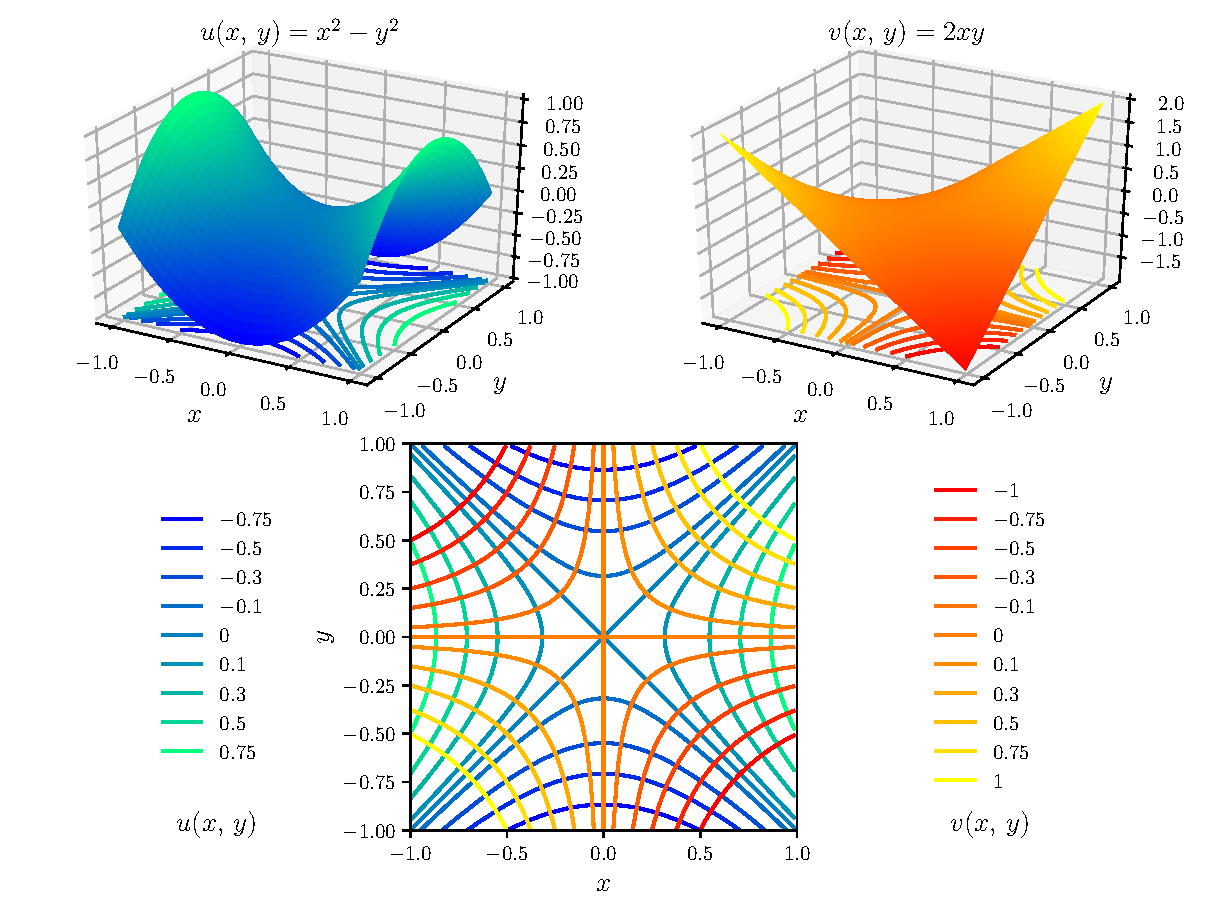
\includegraphics[width=\textwidth]{figuras/exercise_27_2_example.pdf}
 \caption{\label{fig:exercise_27_2_example} Superficie y curvas de nivel de las funciones componentes \(u(x,\,y)=x^2-y^2\) y \(v(x,\,y)=2xy\) de la función \(f(z)=z^2\). Las tangentes a las curvas de nivel de ambos componentes son perpendiculares en los puntos de intersección, excepto en el punto \((0,\,0)\), donde se cumple que \(f'(0)=0\).}
 \end{center}
\end{figure}

\subsubsection{Ejercicio 3}

Mostrar que cuando \(f(z)=z^2\), las curvas de nivel \(u(x,\,y)=c_1\) y \(v(x,\,y)=c_2\) de las funciones componentes son las hipérbolas indicadas en la figura \ref{fig:exercise_27_2_example}. Observar la ortogonalidad de las dos familias, descripta en el Ejercicio 2. Observar que las curvas \(u(x,\,y)=0\) y \(v(x,\,y)=0\) se intersectan en el origen pero no son ortogonales entre si. ¿Porque este hecho es acorde al resultado del Ejercicio 2? 

\paragraph{Solución.} El hecho de que las curvas de nivel 
\[
 u(x,\,y)=x^2-y^2=c_1
 \qquad\qquad\textrm{y}\qquad\qquad
 v(x,\,y)=2xy=c_2
\]
de las funciones componentes de \(f(z)=z^2\) son las hipérbolas mostradas en la figura \ref{fig:exercise_27_2_example} se explicó en la sección \ref{sec:square_mapping}.

Como se explicó en el Ejercicio 2, las curvas de nivel \(u(x,\,y)=0\) y \(v(x,\,y)=0\) se intersectan en el origen pero no son ortogonales debido a que \(f'(0)=0\).

\subsubsection{Ejercicio 4}

Bosquejar las familias de curvas de nivel de las funciones componentes \(u\) y \(v\) cuando \(f(z)=1/z\) y notar la ortogonalidad descripta en el Ejercicio 2.

\paragraph{Solución.} Como
\[
 f(z)=\frac{1}{z}=\frac{\overline{z}}{z\overline{z}}=\frac{\overline{z}}{|z|^2}=\frac{x-iy}{x^2+y^2},
\]
las funciones componentes son
\[
 u(x,\,y)=\frac{x}{x^2+y^2}
 \qquad\qquad\textrm{y}\qquad\qquad
 v(x,\,y)=-\frac{y}{x^2+y^2}.
\]
La ecuación de la curva de nivel 
\[
 u(x,\,y)=\frac{x}{x^2+y^2}=c_1
\]
se puede escribir como
\[
 x^2+y^2-\frac{x}{c_1}=0,
\]
y es equivalente a
\[
 x^2-2\left(\frac{1}{2c_1}\right)x+\left(\frac{1}{2c_1}\right)^2+y^2=\left(\frac{1}{2c_1}\right)^2
\]
o
\[
 \left(x-\frac{1}{2c_1}\right)^2+y^2=\left(\frac{1}{2c_1}\right)^2.
\]
Esto es la ecuación de una circunferencia de centro \([1/(2c_1),\,0]\) y radio \(1/(2c_1)\). Por lo tanto, las curvas de nivel del componente \(u\) son la familia de circunferencias con centro en el eje real \(y=0\) que pasan por el origen \((0,\,0)\), y se muestra en la figura \ref{fig:exercise_27_4}.
\begin{figure}[!htb]
 \begin{center}
 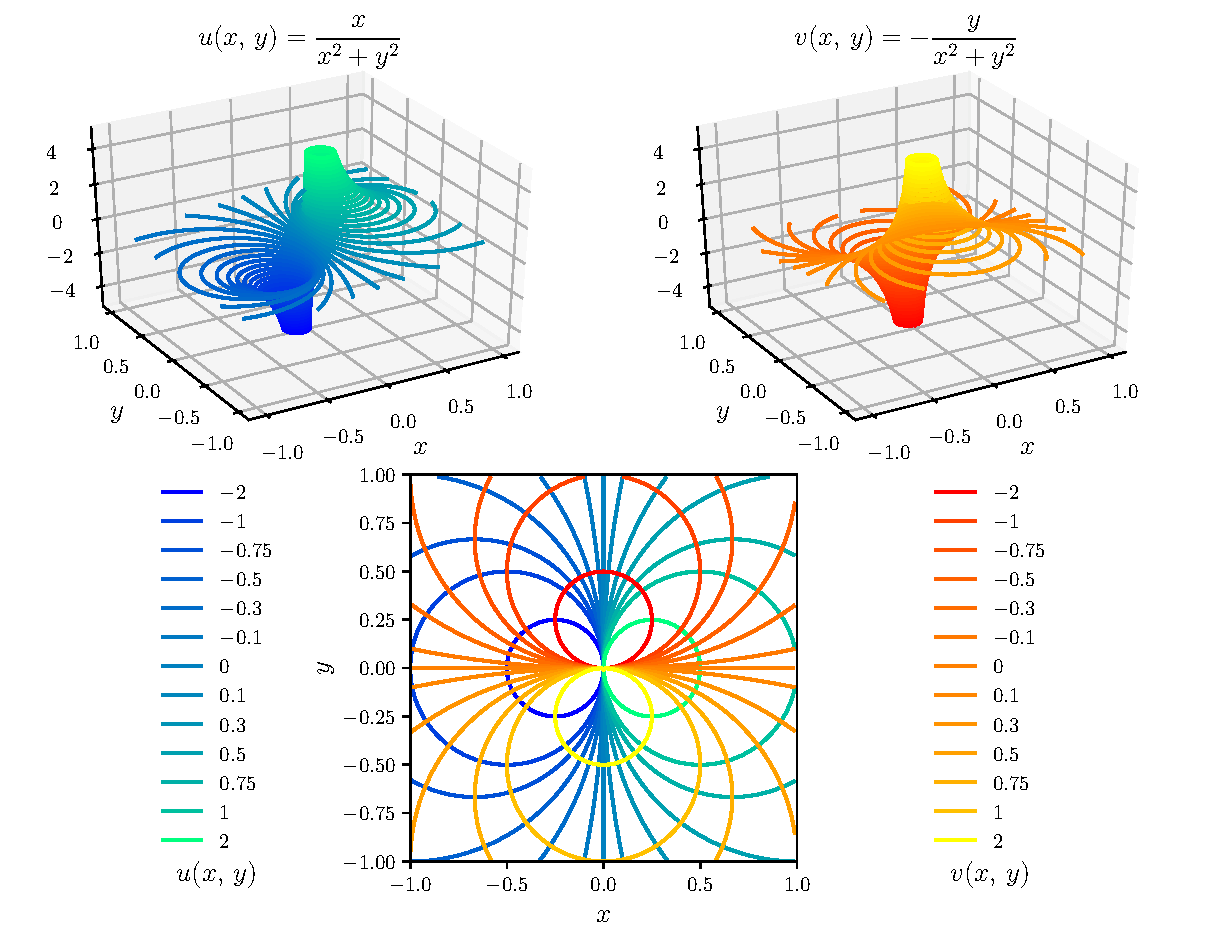
\includegraphics[width=\textwidth]{figuras/exercise_27_4.pdf}
 \caption{\label{fig:exercise_27_4} Superficie y curvas de nivel de las funciones componentes \(u(x,\,y)=x/(x^2+y^2)\) y \(v(x,\,y)=-y/(x^2+y^2)\) de la función \(f(z)=1/z\). Las curvas de nivel del componente \(u\) es la familia de circunferencias con centro en el eje real que pasan por el origen y las curvas de nivel del componente \(v\) es la familia de circunferencias con centro en el eje imaginario que pasan por el origen. Se observa que ambas familas son ortogonales.}
 \end{center}
\end{figure}

Realizando un razonamiento análogo, la ecuación de las curvas de nivel del componente \(v\) 
\[
 v(x,\,y)=-\frac{y}{x^2+y^2}=c_2
\]
es
\[
 x^2+\left(y+\frac{1}{2c_2}\right)^2=\left(\frac{1}{2c_2}\right)^2.
\]
Esto es la ecuación de una circunferencia de centro \([0,\,-1/(2c_2)]\) y radio \(1/(2c_2)\). Por lo tanto, las curvas de nivel del componente \(v\) son la familia de circunferencias con centro en el eje imaginario \(x=0\) que pasan por el origen \((0,\,0)\), como se muestra en la figura \ref{fig:exercise_27_4}. Como se aprecia en la figura, ambas familias de curvas son ortogonales.

\subsubsection{Ejercicio 5}

Hacer el Ejercicio 4 empleando coordenadas polares. 

\paragraph{Solución.} Con \(z=re^{i\theta}\), la función se puede expresar como
\[
 f(z)=\frac{1}{z}=\frac{1}{re^{i\theta}}=\frac{e^{-i\theta}}{r}=\frac{\cos\theta}{r}-i\frac{\sen\theta}{r},
\]
resultando en que las funciones componentes en coordenadas polares son
\[
 u(r,\,\theta)=\frac{\cos\theta}{r}
 \qquad\qquad\textrm{y}\qquad\qquad
 v(r,\,\theta)=-\frac{\sen\theta}{r}.
\]
Para realizar el análisis de las curvas de nivel, se parte considerando que la ecuación de una circunferencia en coordenadas polares es\footnote{Ver \url{https://en.wikipedia.org/wiki/Circle\#Equations}, por ejemplo.}
\[
 r^2-2rr_0\cos(\theta-\varphi)+r_0^2=a^2,
\]
donde \(a\) es el radio, \((r_0,\,\varphi)\) son las coordenadas polares del centro y \((r,\,\theta)\) son las coordenadas polares de los puntos de la circunferencia. En el caso particular en que el origen pertenece a la circunferencia, se cumple que \(r_0=a\), y la ecuación se reduce a
\begin{equation}\label{eq:circunsference_equation_polar_origin}
 r=2r_0\cos(\theta-\varphi).
\end{equation}

Las ecuaciones de las curvas de nivel del componente \(u\) son
\[
 u(r,\,\theta)=\frac{\cos\theta}{r}=c_1,
\]
que se pueden escribir como
\[
 r=\frac{\cos\theta}{c_1}
 \qquad\qquad\textrm{o}\qquad\qquad
 r=\left\{ 
 \begin{array}{ll}
  2\left(\dfrac{1}{2c_1}\right)\cos\theta & c_1\geq0\\[\bigskipamount]
  -2\left(\dfrac{1}{2|c_1|}\right)\cos\theta=2\left(\dfrac{1}{2|c_1|}\right)\cos(\theta-\pi) & c_1<0
 \end{array}
 \right.,
\]
donde se empleó la identidad trigonométrica \(-\cos\theta=\cos(\theta-\pi)\).
Comparando este resultado con el de la ecuación \ref{eq:circunsference_equation_polar_origin}, se concluye que las curvas de nivel son circunferencias de radio \(1/(2|c_1|)\) y centro con coordenadas polares \([1/(2c_1),\,0]\) si \(c_1\geq0\) o \([1/(2|c_1|),\,\pi]\) si \(c_1<0\), es decir, la familia de circunferencias con centro en el eje real que pasan por el origen.

Las ecuaciones de las curvas de nivel del componente \(v\) son
\[
 v(r,\,\theta)=-\frac{\sen\theta}{r}=c_2,
\]
que se pueden escribir como
\[
 r=-\frac{\sen\theta}{c_2}
 \qquad\qquad\textrm{o}\qquad\qquad
 r=\left\{ 
 \begin{array}{ll}
  2\left(\dfrac{1}{2c_2}\right)\cos\left(\theta+\dfrac{\pi}{2}\right) & c_2\geq0\\[\bigskipamount]
  2\left(\dfrac{1}{2|c_2|}\right)\sen\theta=2\left(\dfrac{1}{2|c_2|}\right)\cos\left(\theta-\dfrac{\pi}{2}\right) & c_2<0
 \end{array}
 \right.
\]
donde se empleó la identidad trigonométrica \(\mp\sen\theta=\cos(\theta\pm\pi/2)\). Comparando este resultado con el de la ecuación \ref{eq:circunsference_equation_polar_origin}, se concluye que las curvas de nivel son circunferencias de radio \(1/(2|c_2|)\) y centro con coordenadas polares \([1/(2c_2),\,-\pi/2]\) si \(c_2\geq0\) o \([1/(2|c_2|),\,\pi/2]\) si \(c_2<0\), es decir, la familia de circunferencias con centro en el eje imaginario que pasan por el origen. Las curvas de nivel de ambos componentes se muestran en la figura \ref{fig:exercise_27_4}.

\subsubsection{Ejercicio 6}

Esbozar la familia de curvas de nivel de las funciones componentes \(u\) y \(v\) cuando 
\[
 f(z)=\frac{z-1}{z+1}
\]
y notar como se ilustra en este caso el resultado del Ejercicio 2.

\paragraph{Solución.} Para calcular los componentes se observa que 
\[
 f(z)=\frac{z-1}{z+1}=\frac{(z-1)\overline{(z+1)}}{(z+1)\overline{(z+1)}}
  =\frac{(z-1)(\overline{z}+1)}{|z+1|^2}
  =\frac{z\overline{z}+z-\overline{z}-1}{|z+1|^2}
  =\frac{|z|^2+z-\overline{z}-1}{|z+1|^2}.
\]
Considerando que \(|z|^2=x^2+y^2\), \(|z+1|^2=(x+1)^2+y^2\) y \(z-\overline{z}=2iy\) se obtiene que 
\[
 f(z)=\frac{x^2+y^2-1+2iy}{(x+1)^2+y^2}
\]
por lo que los componentes son
\[
 u(x,\,y)=\frac{x^2+y^2-1}{(x+1)^2+y^2}
 \qquad\qquad\textrm{y}\qquad\qquad
 v(x,\,y)=\frac{2y}{(x+1)^2+y^2}.
\]

Las curvas de nivel del componente \(u\) están dadas por 
\[
 \frac{x^2+y^2-1}{(x+1)^2+y^2}=c_1
 \qquad\Leftrightarrow\qquad
 x^2+y^2-1=c_1[(x+1)^2+y^2]
 \qquad\Leftrightarrow\qquad
 x^2+y^2-1=c_1(x^2+2x+1+y^2)
\]
resultando en que 
\[
 x^2(c_1-1)+2c_1x+(c_1+1)+y^2(c_1-1)=0,
\]
es decir,
\begin{equation}\label{eq:exercise_26_07_u}
 x^2+\frac{2c_1x}{c_1-1}+\frac{c_1+1}{c_1-1}+y^2=0.
\end{equation}
Empleando la técnica de completar el cuadrado, considerando la identidad 
\[
 \left(x+\frac{c_1}{c_1-1}\right)^2=x^2+\frac{2c_1x}{c_1-1}+\frac{c_1^2}{(c_1-1)^2},
\]
la ecuación \ref{eq:exercise_26_07_u} queda 
\[
 \left(x+\frac{c_1}{c_1-1}\right)^2+y^2-\frac{c_1^2}{(c_1-1)^2}+\frac{c_1+1}{c_1-1}=0
\]
resultando en
\[
 \left(x+\frac{c_1}{c_1-1}\right)^2+y^2=\frac{1}{(c_1-1)^2}
\]
Esto es una circunferencia de centro \([-c_1/(c_1-1),\,0]\) y radio \(1/|c_1-1|\). Se observa además que el punto \((-1,\,0)\) pertenece a la circunferencia. Se concluye que las curvas de nivel del componente \(u\) es la familia de circunferencias con centro en el eje real que pasan por el punto \((-1,\,0)\) y se muestran en la figura \ref{fig:exercise_27_6}.
\begin{figure}[!htb]
 \begin{center}
 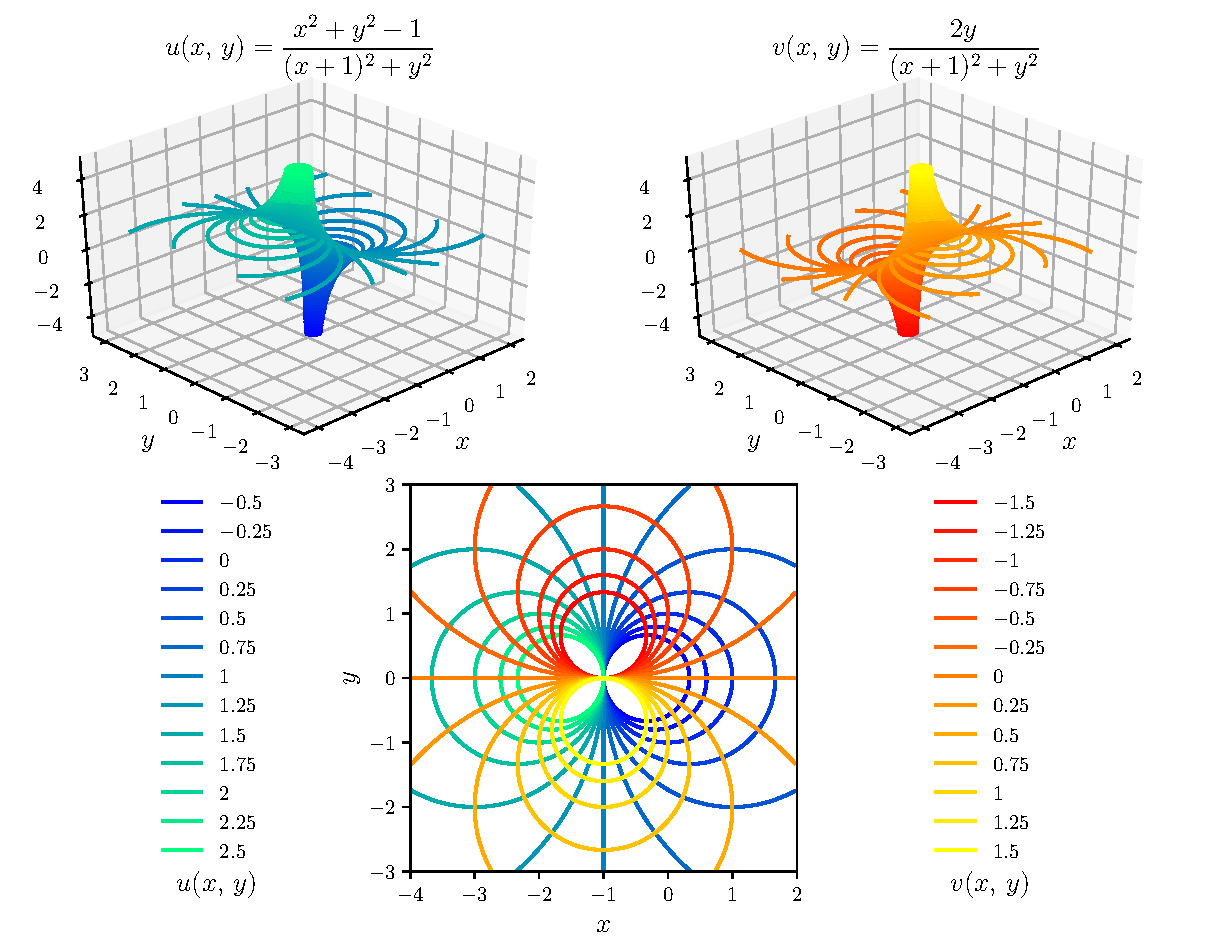
\includegraphics[width=\textwidth]{figuras/exercise_27_6.pdf}
 \caption{\label{fig:exercise_27_6} Superficie y curvas de nivel de las funciones componentes \(u(x,\,y)\) y \(v(x,\,y)\) de la función \(f(z)=(z-1)/(z+1)\). Las curvas de nivel del componente \(u\) es la familia de circunferencias con centro en el eje real que pasan por el punto \((-1,\,0)\) y las curvas de nivel del componente \(v\) es la familia de circunferencias con centro en la recta vertical \(x=-1\) que pasan por el punto \((-1,\,0)\). Se observa que ambas familas son ortogonales.}
 \end{center}
\end{figure}

Las curvas de nivel del componente \(v\) están dadas por 
\[
 \frac{2y}{(x+1)^2+y^2}=c_2,
\]
es decir,
\begin{equation}\label{eq:exercise_26_07_v}
 (x+1)^2+y^2-\frac{2y}{c_2}=0.
\end{equation}
Nuevamente, empleando la técnica de completar el cuadrado, como
\[
 \left(y-\frac{1}{c_2}\right)^2=y^2-\frac{2y}{c_2}+\frac{1}{c_2^2},
\]
la ecuación \ref{eq:exercise_26_07_v} se puede escribir como
\[
 (x+1)^2+\left(y-\frac{1}{c_2}\right)^2=\frac{1}{c_2^2}.
\]
Esto es una circunferencia de centro \((-1,\,1/c_2)\) y radio \(1/|c_2|\). Se observa además que el punto \((-1,\,0)\) pertenece a la circunferencia. Se concluye que las curvas de nivel del componente \(v\) es la familia de circunferencias con centro en la recta vertical \(x=-1\) que pasan por el punto \((-1,\,0)\) y se muestran en la figura \ref{fig:exercise_27_6}.

\section{Funciones analíticas determinadas unívocamente}\label{sec:uniquely_determined_analytic_functions}

En esta sección y la siguiente se estudia como los valores de una función analítica en un dominio \(D\) son afectados por sus valores en un subdominio de \(D\) o en un segmento de recta en \(D\). 

\paragraph{Lema.} Supóngase que 
\begin{enumerate}
 \item[(\textit{a})] una función \(f\) es analítica en un dominio \(D\);
 \item[(\textit{b})] \(f(z)=0\) en un dominio o segmento de recta contenido en \(D\)
\end{enumerate}
Entonces, se cumple que \(f(z)\equiv0\) en \(D\), es decir, \(f(z)\) es idénticamente nula en \(D\).

Por la demostración de este lema recurrir a \cite{brown2013complex}, aunque el enfoque general de la prueba es similar a la del teorema de la sección \ref{sec:maximum_modulus_principle}.

Supóngase ahora que dos funciones \(f\) y \(g\) son analíticas en el mismo dominio \(D\) y \(f(z)=g(z)\) en un dominio o segmento de recta contenido en \(D\). La diferencia
\[
 h(z)=f(z)-g(z)
\]
también es analítica en \(D\) y \(h(z)=0\) en el dominio o segmento. De acuerdo al lema, \(h(z)\equiv0\) en \(D\) y por lo tanto, \(f(z)=h(z)\) en cada punto de \(D\). Esto conduce al siguiente importante teorema.

\paragraph{Teorema.} Una función que es analítica en \(D\) está unívocamente determinada en \(D\) por los valores en un dominio o segmento de recta contenido en \(D\).

Este teorema es útil en el estudio de la extensión del dominio de definición de una función analítica. Mas precisamente, dados dos dominios \(D_1\) y \(D_2\), se considera la intersección \(D_1\cap D_2\). Si \(D_1\) y \(D_2\) tienen puntos en común y una función \(f_1\) es analítica en \(D_1\) \emph{puede} existir una función \(f_2\) analítica en \(D_2\) tal que \(f_2(z)=f_1(z)\) para cada \(z\) en la intersección \(D_1\cap D_2\). En ese caso \(f_2\) se llama \emph{continuación analítica} de \(f_1\) en el dominio \(D_2\).
\begin{figure}[!htb]
  \begin{minipage}[c]{0.4\textwidth}
    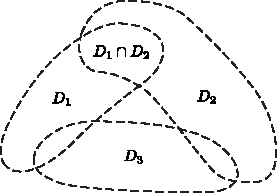
\includegraphics[width=\textwidth]{figuras/analytic_continuation.pdf}
  \end{minipage}\hfill
  \begin{minipage}[c]{0.5\textwidth}
    \caption{
       Continuación analítica.
    } \label{fig:analytic_continuation}
  \end{minipage}
\end{figure}

Si la continuación analítica existe, por el teorema anterior, es única. Es decir, no mas de una función puede ser analítica en \(D_2\) y asumir el valor \(f_1(z)\) en cada punto \(z\) del dominio \(D_1\cap D_2\) interior a \(D_2\). Sin embargo, si hay una continuación analítica \(f_3\) de \(f_2\) del dominio \(D_2\) al dominio \(D_3\) que intersecta al dominio \(D_1\), como se muestra en la figura \ref{fig:analytic_continuation}, no es necesariamente cierto que \(f_3(z)=f_1(z)\) para cada \(z\) en \(D_1\cap D_3\). Esto se ilustra en el Ejercicio 2 de la sección \ref{sec:reflection_principle}. 

Si \(f_2\) es la continuación analítica de \(f_1\) de un dominio \(D_1\) a un dominio \(D_2\), la función \(F\) definida como
\[
 F(z)=
 \left\{ 
 \begin{array}{ll}
  f_1(z) & \textrm{si }z\in D_1\\[\smallskipamount]
  f_2(z) & \textrm{si }z\in D_2,
 \end{array}
 \right.
\]
es analítica en la unión \(D_1\cup D_2\). La función \(F\) es la continuación analítica en \(D_1\cup D_2\) de \(f_1\) o \(f_2\), y \(f_1\) y \(f_2\) se dicen \emph{elementos} de \(F\).

\section{Principio de reflexión}\label{sec:reflection_principle}

El teorema en esta sección concierne al hecho de que algunas funciones analíticas tienen la propiedad de que \(\overline{f(z)}=f(\overline{z})\) en todos los puntos \(z\) de algunos dominios, mientras otras no. Se observa por ejemplo que las funciones \(z+1\) y \(z^2\) tienen esta propiedad cuando el dominio \(D\) es el plano complejo finito, pero lo mismo no es cierto para las funciones \(z+i\) y \(iz^2\). El siguiente teorema, denominado \emph{principio de reflexión} provee una forma de predecir cuando \(\overline{f(z)}=f(\overline{z})\). 

\paragraph{Teorema.} Supóngase que una función \(f\) es analítica en un dominio \(D\) que contiene un segmento del eje \(x\) y cuya mitad inferior es el reflejo de la mitad superior respecto al eje \(x\). Entonces 
\begin{equation}\label{eq:reflection_principle}
 \overline{f(z)}=f(\overline{z})
\end{equation}
para cada punto \(z\) en el dominio si y solo si \(f(x)\) es real para cada punto \(x\) en el segmento del eje real.

Se comienza la prueba asumiendo que \(f(x)\) es real en cada punto \(x\) del segmento. Se mostrará que 
\begin{equation}\label{eq:reflection_principle_proof_F}
 F(z)=\overline{f(\overline{z})}
\end{equation}
es analítica en \(D\), y se empleará ese resultado junto con la hipótesis para obtener \ref{eq:reflection_principle}. Para obtener la analiticidad de \(F(x)\) se escribe
\[
 f(z)=u(x,\,y)+iv(x,\,y)
 \qquad\qquad\textrm{y}\qquad\qquad
 F(z)=U(x,\,y)+iV(x,\,y).
\]
De esta forma,
\begin{equation}\label{eq:reflection_principle_f_reflected_components}
 \overline{f(\overline{z})}=u(x,\,-y)-iv(x,\,-y) 
\end{equation}
y por lo tanto, los componentes de \(F(z)\) y \(f(z)\) se relacionan por las ecuaciones
\[
 U(x,\,y)=u(x,\,-y)
 \qquad\qquad\textrm{y}\qquad\qquad
 V(x,\,y)=-v(x,\,-y).
\]
o, definiendo \(t=-y\),
\begin{equation}\label{eq:reflection_principle_proof_F_f_relation}
 U(x,\,y)=u(x,\,t)
 \qquad\qquad\textrm{y}\qquad\qquad
 V(x,\,y)=-v(x,\,t).
\end{equation}
Continuando, como por hipótesis \(f(x+it)\) es una función analítica de \(x+it\), las derivadas parciales de primer orden de las funciones componentes \(u(x,\,t)\) y \(v(x,\,t)\) son continuas en \(D\) y satisfacen las ecuaciones de Cauchy-Riemann, 
\begin{equation}\label{eq:reflection_principle_proof_cr_f}
 u_x=v_t
 \qquad\qquad\textrm{y}\qquad\qquad
 u_t=-v_x, 
\end{equation}
como se demostró en la sección \ref{sec:differentiability_sufficient_conditions}. Además, de las ecuaciones \ref{eq:reflection_principle_proof_F_f_relation},
\begin{equation}\label{eq:reflection_principle_proof_F_f_derivatives_1}
  U_x=u_x
 \qquad\qquad\textrm{y}\qquad\qquad
 V_y=\frac{\partial(-v)}{\partial t}\frac{dt}{dy}=(-v_t)(-1)=v_t,
\end{equation}
y de forma similar,
\begin{equation}\label{eq:reflection_principle_proof_F_f_derivatives_2}
 U_y=\frac{\partial u}{\partial t}\frac{dt}{dy}=(u_t)(-1)=-u_t
 \qquad\qquad\textrm{y}\qquad\qquad
 V_x=-v_x.
\end{equation}
Combinando las ecuaciones en \ref{eq:reflection_principle_proof_F_f_derivatives_1} con la primer ecuación en \ref{eq:reflection_principle_proof_cr_f} se obtiene que \(U_x=V_y\), y combinando las ecuaciones en \ref{eq:reflection_principle_proof_F_f_derivatives_2} con la segunda ecuación en \ref{eq:reflection_principle_proof_cr_f} se obtiene que \(U_y=-V_x\). Se obtuvo que las derivadas parciales de \(U(x,\,y)\) y \(V(x,\,y)\) satisfacen las ecuaciones de Cauchy-Riemann, y como esas derivadas son continuas, se concluye que \(F(z)\) es analítica en \(D\). Además, como \(f(x)\) es real en el segmento del eje real en \(D\), se cumple que \(v(x,\,0)=0\) en el segmento, y de las ecuaciones \ref{eq:reflection_principle_proof_F_f_relation}, se observa que 
\[
 F(x)=U(x,\,0)+iV(x,\,0)=u(x,\,0)-iv(x,\,0)=u(x,\,0)=f(x),
\]
es decir,
\begin{equation}\label{eq:reflection_principle_proof_conclution}
 F(z)=f(z)
\end{equation}
en cada punto del segmento. Por lo tanto, del teorema de la sección \ref{sec:uniquely_determined_analytic_functions} que indica que una función analítica definida en un dominio \(D\) queda determinada por unívocamente por los valores en cualquier segmento en \(D\) se concluye que la ecuación \ref{eq:reflection_principle_proof_conclution} es válida en todo el dominio \(D\). De la definición \ref{eq:reflection_principle_proof_F} de la función \(F(z)\) se obtiene que 
\begin{equation}\label{eq:reflection_principle_alt}
 \overline{f(\overline{z})}=f(z), 
\end{equation}
que es lo mismo que la ecuación \ref{eq:reflection_principle}, concluyendo la prueba.

Para probar el recíproco del teorema, se asume que se cumple la ecuación \ref{eq:reflection_principle}. De la ecuación \ref{eq:reflection_principle_f_reflected_components}, la forma \ref{eq:reflection_principle_alt} de la ecuación \ref{eq:reflection_principle} se puede escribir como 
\[
 u(x,\,-y)-iv(x,\,-y)=u(x,\,y)+iv(x,\,y)
\]
En particular, si \((x,\,0)\) es un punto del segmento del eje real en \(D\),
\[
 u(x,\,0)-iv(x,\,0)=u(x,\,0)+iv(x,\,0),
\]
e igualando las partes imaginarias, se obtiene que \(v(x,\,0)=0\). Se concluye que \(f(x)\) es real en el segmento del eje real en \(D\). 

\subsection*{Ejercicios}

\subsubsection{Ejercicio 1}

Emplear el teorema de la sección \ref{sec:uniquely_determined_analytic_functions} para mostrar que si  \(f(z)\) es analítica y no constante en un dominio \(D\), no puede ser constante en ningún entorno en \(D\).

\emph{Sugerencia:} suponer que \(f(z)\) tiene un valor constante \(w_0\) en algún entorno en \(D\).

\paragraph{Solución.} \(f(z)\) es analítica en \(D\) y por absurdo, supóngase que \(f(z)=w_0\) constante en un entorno en \(D\). De esta forma, la función \(h(z)=f(z)-w_0\) es analítica en \(D\) y \(h(z)=0\) en dicho entorno en \(D\). Del lema de la sección \ref{sec:uniquely_determined_analytic_functions}, se debe  cumplir que \(h(z)=0\) en todo \(D\), o equivalentemente, \(f(z)=w_0\) constante en todo \(D\), contradiciendo la hipótesis. Se concluye que \(f(z)\) no puede ser constante en ningún entorno en \(D\).

\subsubsection{Ejercicio 2}

Comenzando con la función
\[
 f_1(z)=\sqrt{r}e^{i\theta/2}\qquad\textrm{con}\qquad r>0,\,0<\theta<\pi,
\]
y refiriéndose al ejemplo de la sección \ref{sec:cauchy_riemann_equations_polar} indicar porque
\[
 f_2(z)=\sqrt{r}e^{i\theta/2}\qquad\textrm{con}\qquad r>0,\,\frac{\pi}{2}<\theta<2\pi,
\]
es una continuación analítica de \(f_1\) al eje real negativo y el semiplano inferior. Luego, mostrar que la función 
\[
 f_3(z)=\sqrt{r}e^{i\theta/2}\qquad\textrm{con}\qquad r>0,\,\pi<\theta<\frac{5\pi}{2},
\]
es una continuación analítica de \(f_2\) al eje real positivo y al primer cuadrante, pero \(f_3(z)=-f_1(z)\) allí.

\paragraph{Solución.} En el ejemplo de la sección \ref{sec:cauchy_riemann_equations_polar} se mostró que la función 
\[
 f(z)=\sqrt{r}e^{i\theta/2}\qquad\textrm{con}\qquad r>0,\,\alpha<\theta<\alpha+2\pi,
\]
es analítica en todo el dominio de definición. 

El dominio de definición \(D_1\) de la función \(f_1\) es el semiplano superior, y la función es analítica allí. Por otro lado, el dominio de definición \(D_2\) de la función \(f_2\) es el segundo cuadrante y el semiplano inferior, y es analítica allí. Se cumple entonces que 
\[
 D_1\cap D_2=\left\{r>0,\,\frac{\pi}{2}<\theta<\pi\right\}
\]
y además \(f_2(z)=f_1(z)\) para cada \(z\) en \(D_1\cap D_2\). Por lo tanto, \(f_2\) es la continuación analítica de \(f_1\) del semiplano superior al eje real negativo y el semiplano inferior.

De forma similar, el dominio \(D_3\) de la función \(f_3\) es el semiplano inferior y el primer cuadrante, y la función es analítica en todo el dominio. De esta forma, se cumple que 
\[
 D_2\cap D_3=\left\{r>0,\,\pi<\theta<2\pi\right\}
\]
y además, como \(f_3(z)=f_2(z)\) para cada \(z\) en \(D_2\cap D_3\), \(f_3\) es la continuación analítica de \(f_2\) al eje real positivo y al primer cuadrante.

Finalmente, se observa que los dominios \(D_1\) y \(D_3\) contienen al primer cuadrante. Efectivamente, en el dominio \(D_1\) los puntos del primer cuadrante se obtienen con \(0<\theta<\pi/2\), y en el dominio \(D_3\) los puntos del primer cuadrante se obtienen con \(2\pi<\theta<5\pi/4=2\pi+\pi/2\). Sea el punto \(z=re^{i\theta}\) con \(0<\theta<\pi/2\) y sea el punto \(z'=re^{i\theta'}\) con \(\theta'=\theta+2\pi\). De esta forma, \(z\in D_1\), \(z'\in D_3\) y además \(z'=z\), ya que
\[
 z'=re^{i\theta'}=re^{i(\theta+2\pi)}=re^{i\theta}e^{i2\pi}=re^{i\theta}=z.
\]
Se cumple que 
\[
 f_1(z)=\sqrt{r}e^{i\theta/2},
\]
y
\[
 f_3(z)=f_3(z')=\sqrt{r}e^{i\theta'/2}=\sqrt{r}e^{i(\theta+2\pi)/2}=\sqrt{r}e^{i\theta/2}e^{i\pi}=\sqrt{r}e^{i\theta/2}(-1)=-f_1(z).
\]
Se concluye que \(f_2\) es la continuación analítica de \(f_1\), \(f_3\) es la continuación analítica de \(f_2\) pero \(f_3\) no es la continuación analítica de \(f_1\) en \(D_1\cap D_3\).

\subsubsection{Ejercicio 3}

Indicar porque la función 
\[
 f_4(z)=\sqrt{r}e^{i\theta/2}\qquad\textrm{con}\qquad r>0,\,-\pi<\theta<\pi,
\]
es la continuación analítica de \(f_1\) del Ejercicio 2 al eje real positivo y el semiplano inferior.

\paragraph{Solución.} El dominio de definición \(D_1\) de la función \(f_1\) es el semiplano superior, y la función es analítica allí. Por otro lado, el dominio de definición \(D_4\) de la función \(f_4\) es todo el plano excepto el eje real negativo, y es analítica allí. Se cumple entonces que 
\[
 D_1\cap D_4=\left\{r>0,\,0<\theta<\pi\right\}
\]
y además \(f_4(z)=f_1(z)\) para cada \(z\) en \(D_1\cap D_4\). Por lo tanto, \(f_4\) es la continuación analítica de \(f_1\) del semiplano superior al semiplano inferior y al eje real positivo.

\subsubsection{Ejercicio 4}

Del ejemplo de la sección \ref{sec:differentiability_sufficient_conditions} se sabe que la función 
\[
 f(z)=e^z=e^x\cos y+ie^x\sen y
\]
es diferenciable en todos lados en el plano complejo finito. Indicar como surge del principio de reflexión que 
\[
 \overline{f(z)}=f(\overline{z})
\]
para todo \(z\). Luego, verificarlo directamente.

\paragraph{Solución.} Como el dominio de la función es todo el plano complejo, contiene todo el eje real, y la mitad inferior, que es todo el semiplano inferior, es el reflejo de la mitad superior, que es todo el semiplano superior. De esta forma el dominio cumple las condiciones del principio de reflexión. Como para un punto \(z=x+i0\) del eje real, la función toma el valor
\[
 f(z)=f(x)=e^x
\]
real, por el teorema de reflexión se cumple que \(\overline{f(z)}=f(\overline{z})\) para todo \(z\).

Para verificar el resultado de forma directa, se observa que 
\[
 \overline{f(z)}=e^x\cos y-ie^x\sen y,
\]
y además, con \(\overline{z}=x-iy\),
\[
 f(\overline{z})=e^x\cos(-y)+ie^x\sen(-y)=e^x\cos y-ie^x\sen y,
\]
resultando en que \(\overline{f(z)}=f(\overline{z})\) para todo \(z\).

\subsubsection{Ejercicio 5}

Mostrar que si la condición de que \(f(x)\) es real en el principio de reflexión se reemplaza por la condición de que \(f(x)\) es imaginario puro, la ecuación \ref{eq:reflection_principle} del principio cambia a 
\begin{equation}\label{reflection_principle_imaginary}
 \overline{f(z)}=-f(\overline{z}).
\end{equation}

\paragraph{Solución.} Como se demostró en el teorema del principio de reflexión en la sección \ref{sec:reflection_principle}, la función
\begin{equation}\label{eq:exercise_26_05_F}
 F(z)=\overline{f(\overline{z})}
\end{equation}
es analítica en el dominio de definición \(D\) de \(f\). Para demostrar el teorema directo, supóngase que \(f(x)\) es imaginario puro en el segmento del eje real en \(D\). De esta forma, el componente real de \(f(z)\) es nulo en los puntos del segmento del eje real, es decir, \(u(x,\,0)=0\). Por lo tanto, de la ecuación \ref{eq:reflection_principle_proof_F_f_relation} en el teorema,
\[
 F(x)=U(x,\,0)+iV(x,\,0)=u(x,\,0)-iv(x,\,0)=-iv(x,\,0)=-f(x),
\]
es decir,
\begin{equation}\label{eq:exercise_26_05_F_f}
 F(z)=-f(z)
\end{equation}
en cada punto del segmento. Por lo tanto, del teorema de la sección \ref{sec:uniquely_determined_analytic_functions} que indica que una función analítica definida en un dominio \(D\) queda determinada por unívocamente por los valores en cualquier segmento en \(D\) se concluye que la ecuación \ref{eq:exercise_26_05_F_f} es válida en todo el dominio \(D\). De la definición \ref{eq:exercise_26_05_F} de la función \(F(z)\) se obtiene que
\begin{equation}\label{reflection_principle_imaginary_alt}
 \overline{f(\overline{z})}=-f(z), 
\end{equation}
que es lo mismo que la ecuación \ref{reflection_principle_imaginary}.

Para demostrar el recíproco, se asume que se cumple la ecuación \ref{reflection_principle_imaginary}, que se puede expresar como
\[
 u(x,\,y)-iv(x,\,y)=-u(x,\,-y)-iv(x,\,-y).
\]
En particular, si \((x,\,0)\) es un punto del segmento del eje real en \(D\),
\[
 u(x,\,0)-iv(x,\,0)=-u(x,\,0)-iv(x,\,0),
\]
e igualando las partes reales, se obtiene que \(u(x,\,0)=0\). Se concluye que \(f(x)\) es imaginario puro en el segmento del eje real en \(D\).

\chapter{Funciones elementales}

En este capítulo se consideran varias funciones elementales estudiadas en cálculo y se definen las  correspondientes funciones de variable compleja. Específicamente, se definen funciones analíticas de una variable compleja \(z\) que se reduce a una función elemental en cálculo cuando \(z=x+i0\).

\section{La función exponencial}\label{sec:exponential_function}

La función exponencial se define como
\[
 e^z=e^xe^{iy}=e^x(\cos y+i\sen y),\qquad\qquad\textrm{con}\qquad\qquad z=x+iy.
\]
Se observa que \(e^z\) se reduce a la función exponencial usual de cálculo cuando \(y=0\).

Hay varias propiedades que se extienden de \(e^x\) a \(e^z\). Algunas de ellas son las siguientes (ver la sección 30 de \cite{brown2013complex}):
\begin{itemize}
 \item \(e^z\neq0\) para todo \(z\).
 \item \(e^{z_1}e^{z_2}=e^{z_1+z_2}\)
 \item \(\dfrac{e^{z_1}}{e^{z_2}}=e^{z_1-z_2}\)
 \item \(\dfrac{d}{dz}e^z=e^z\) en todo el plano complejo. Esto se mostró en el ejemplo de la sección \ref{sec:differentiability_sufficient_conditions}.
\end{itemize}

Por otro lado, algunas propiedades de \(e^z\) no son esperadas. Por ejemplo, como
\[
 e^{z+2\pi i}=e^{z}e^{2\pi i}
  \qquad\qquad\textrm{y}\qquad\qquad
 e^{2\pi i}=1, 
\]
se encuentra que \(e^z\) es \emph{periódica} con período imaginario puro de \(2\pi i\):
\[
 e^{z+2\pi i}=e^{z}.
\]
Otra propiedad de \(e^z\) que no se traslada de \(e^x\) es que si bien \(e^x\) es siempre positivo, \(e^z\) puede ser negativo. Por ejemplo, \(e^{i\pi}=-1\), o mas en general,
\[
 e^{i(2n+1)\pi}=-1,\qquad\textrm{para}\qquad n=0,\,\pm1,\,\pm2,\,\dots.
\]
De hecho, \(e^z\) puede tomar el valor de cualquier número complejo no nulo.

\subsection*{Ejercicios}

\subsubsection{Ejercicio 1}

Mostrar que 
\[
 (\textit{a})\;\exp(2\pm3\pi i)=-e^2;\qquad\qquad 
 (\textit{b})\;\exp\left(\frac{2+\pi i}{4}\right)=\sqrt{\frac{e}{2}}(1+i);\qquad\qquad
 (\textit{c})\;\exp(z+\pi i)=-\exp z.
\]

\paragraph{Solución.} 

\begin{enumerate}
 \item[(\textit{a})] \(\exp(2\pm3\pi i)=e^2e^{\pm3\pi i}=e^2(-1)=-e^2\).
 \item[(\textit{b})] \(\displaystyle\exp\left(\frac{2+\pi i}{4}\right)=\exp\left(\frac{1}{2}\right)\exp\left(\frac{\pi i}{4}\right)=\sqrt{e}\left(\cos\frac{\pi}{4}+i\sen\frac{\pi}{4}\right)=\sqrt{e}\left(\frac{1}{\sqrt{2}}+i\frac{1}{\sqrt{2}}\right)\sqrt{e}(1+i)\).
 \item[(\textit{c})] \(\exp(z+\pi i)=e^ze^{\pi i}=e^z(-1)=-e^z\).
\end{enumerate}

\subsubsection{Ejercicio 2}

Explicar porque la función \(f(z)=2z^2-3-ze^z+e^{-z}\) es completa.

\paragraph{Solución.} \(2z^2-3\) es completa por ser un polinomio, \(ze^z\) es completa por ser el producto de funciones completas y \(e^{-z}=1/e^z\) es completa por ser el cociente de funciones completas y el denominador cumple que \(e^z\neq 0\) para todo \(z\). Se concluye que \(f(z)\) es completa por ser la suma de funciones completas.

\subsubsection{Ejercicio 3}

Emplear las ecuaciones de Cauchy-Riemann y el teorema de la sección \ref{sec:cauchy_riemann_equations} para mostrar que la función \(f(z)=e^{\overline{z}}\) no es analítica en ningún lado.

\paragraph{Solución.} El hecho de que 
\[
 f(z)=e^{\overline{z}}=e^{x-iy}=e^xe^{-iy}
\]
no es analítica en ningún punto se mostró en el ejercicio 1 parte \((d)\) de la sección \ref{sec:cauchy_riemann_equations_polar}.

\subsubsection{Ejercicio 4}

Mostrar de dos formas que la función \(f(z)=\exp(z^2)\) es completa. ¿Cuál es su derivada?

\paragraph{Solución.} Una forma de mostrar que la función 
\[
 f(z)=\exp(z^2)
\]
es completa es considerar que se trata de la composición \(f(z)=g[h(z)]\) de las funciones \(g(z)=e^z\) y \(h(z)=z^2\). Como las funciones \(g\) y \(h\) son completas, la composición \(f(z)=g[h(z)]\) es completa, como se justificó en el ejercicio 3 de la sección \ref{sec:analytic_functions}. Además, por la regla de la cadena, la derivada es
\[
 \frac{d}{dz}g[h(z)]=g'[h(z)]h'(z).
\]
Como en este caso
\[
 g'(z)=e^z
 \qquad\qquad\textrm{y}\qquad\qquad
 h'(z)=2z,
\]
la derivada queda
\[
 f'(z)=e^{z^2}(2z)=2ze^{z^2}.
\]

Una segunda forma de demostrar que la función es completa es empleando el teorema de la sección \ref{sec:differentiability_sufficient_conditions}. Para hacerlo, se parte calculando las funciones componentes. Como
\[
 f(z)=e^{z^2}=e^{x^2-y^2+2ixy}=e^{x^2-y^2}e^{2ixy}=e^{x^2-y^2}(\cos2xy+i\sen2xy),
\]
las funciones componente son
\[
 u(x,\,y)=e^{x^2-y^2}\cos2xy
 \qquad\qquad\textrm{y}\qquad\qquad
 v(x,\,y)=e^{x^2-y^2}\sen2xy.
\]
Para verificar si se cumplen las ecuaciones de Cauchy-Riemann, se calculan las derivadas parciales,
\[
 u_x=2xe^{x^2-y^2}\cos2xy+e^{x^2-y^2}(2y)(-\sen2xy)=2e^{x^2-y^2}(x\cos2xy-y\sen2xy)
\]
\[
 v_y=-2ye^{x^2-y^2}\sen2xy+e^{x^2-y^2}(2x)\cos2xy=2e^{x^2-y^2}(x\cos2xy-y\sen2xy).
\]
Como \(u_x=v_y\), se concluye que se cumple la primera ecuación de Cauchy-Riemann. Además,
\[
 u_y=-2ye^{x^2-y^2}\cos2xy+e^{x^2-y^2}(2x)(-\sen2xy)=-2e^{x^2-y^2}(y\cos2xy+x\sen2xy)
\]
\[
 v_x=2xe^{x^2-y^2}\sen2xy+e^{x^2-y^2}(2y)\cos2xy=2e^{x^2-y^2}(y\cos2xy+x\sen2xy),
\]
concluyendo que la segunda ecuación de Cauchy-Riemann \(u_y=-v_x\) también se cumple. Como las derivadas parciales existen y son continuas en todo el plano y las ecuaciones de Cauchy-Riemann se cumplen en todo el plano, se concluye que la función \(f\) es completa. Finalmente, la derivada es
\begin{align*}
 f'(z)&=u_x+iv_x\\
  &=2e^{x^2-y^2}\left[(x\cos2xy-y\sen2xy)+i(y\cos2xy+x\sen2xy)\right]\\
  &=2e^{x^2-y^2}\left[(x+iy)\cos2xy+(ix-y)\sen2xy\right]\\
  &=2e^{x^2-y^2}\left[(x+iy)\cos2xy+i(x+iy)\sen2xy\right]\\
  &=2(x+iy)e^{x^2-y^2}(\cos2xy+i\sen2xy)\\
  &=2(x+iy)e^{x^2-y^2}e^{2ixy}\\
  &=2(x+iy)e^{x^2-y^2+2ixy}\\
  &=2(x+iy)e^{(x+iy)^2},
\end{align*}
resultando en que
\[
 f'(z)=2ze^{z^2}.
\]

\subsubsection{Ejercicio 5}

Escribir \(|e^{2z+i}|\) y \(|e^{iz^2}|\) en términos de \(x\) y \(y\). Luego mostrar que 
\[
 |e^{2z+i}+e^{iz^2}|\leq e^{2x}+e^{-2xy}.
\]

\paragraph{Solución.} Por un lado se ve que 
\[
 e^{2z+i}=e^{2(x+iy)+i}=e^{2x}e^{i(2y+1)},
\]
y por lo tanto
\[
 |e^{2z+i}|=|e^{2x}||e^{i(2y+1)}|=|e^{2x}|=e^{2x},
\]
donde se consideró que si \(x\) es un número real, se cumple que \(|e^{ix}|=1\) y \(e^x>0\). Por otro lado se tiene que 
\[
 e^{iz^2}=e^{i(x^2-y^2+2ixy)}=e^{-2xy}e^{i(x^2-y^2)}
\]
y por lo tanto
\[
 |e^{iz^2}|=|e^{-2xy}||e^{i(x^2-y^2)}|=|e^{-2xy}|=e^{-2xy}.
\]
Luego,
\[
 |e^{2z+i}+e^{iz^2}|\leq|e^{2z+i}|+|e^{iz^2}|=e^{2x}+e^{-2xy},
\]
donde se empleó la desigualdad triangular y los resultados obtenidos previamente.

\subsubsection{Ejercicio 6}

Mostrar que \(|e^{z^2}|\leq e^{|z|^2}\).

\paragraph{Solución.} Por un lado se ve que 
\[
 e^{z^2}=e^{x^2-y^2+2ixy}=e^{x^2-y^2}e^{2ixy}
\]
y por lo tanto,
\[
 |e^{z^2}|=|e^{x^2-y^2}||e^{2ixy}|=|e^{x^2-y^2}|=e^{x^2-y^2}.
\]
Además,
\[
 e^{|z|^2}=e^{x^2+y^2}
\]
Como \(x^2-y^2\leq x^2+y^2\) y la función exponencial real es creciente, se cumple que 
\[
 e^{x^2-y^2}\leq e^{x^2+y^2},
\]
concluyendo que 
\[
 |e^{z^2}|\leq e^{|z|^2}.
\]

\subsubsection{Ejercicio 7}

Probar que \(|e^{-2z}|<1\) si y solo si \(\Re z>0\).

\paragraph{Solución.} Se observa que
\[
 |e^{-2z}|=|e^{-2(x+iy)}|=|e^{-2x}e^{-2iy}|=|e^{-2x}||e^{-2iy}|=|e^{-2x}|=e^{-2x}.
\]
Como \(e^{-2x}\geq1\) si \(x\leq0\) y \(e^{-2x}<1\) si \(x>0\), y además \(x=\Re z\), se cumple que \(|e^{-2z}|<1\) si y solo si \(\Re z>0\). 

\subsubsection{Ejercicio 8}

Encontrar todos los valores de \(z\) tal que 
\[
 (\textit{a})\;\exp z=-2;\qquad\qquad 
 (\textit{b})\;\exp z=1+i;\qquad\qquad
 (\textit{c})\;\exp(2z-1)=1.
\]

\paragraph{Solución.} 

\begin{enumerate}
 \item[(\textit{a})] 
 \[
  e^z=-2
  \qquad\qquad\Leftrightarrow\qquad\qquad
  e^xe^{iy}=2e^{i(2n+1)\pi},
  \qquad\qquad\textrm{con }n=0,\,\pm1,\,\pm2,\,\dots.
 \]
 Por lo tanto, igualando el módulo y la fase, se tiene que 
 \[
  \begin{array}{l}
   e^x=2\\
   y=(2n+1)\pi
  \end{array}
  \qquad\qquad\Rightarrow\qquad\qquad
  \begin{array}{l}
   x=\ln 2\\
   y=(2n+1)\pi
  \end{array}
  \qquad\qquad\Rightarrow\qquad\qquad
  z=\ln2+i(2n+1)\pi.
 \]
 \item[(\textit{b})] 
 \[
  e^z=1+i
  \qquad\qquad\Leftrightarrow\qquad\qquad
  e^xe^{iy}=\sqrt{2}\exp\left[i\left(\frac{\pi}{4}+2n\pi\right)\right],
  \qquad\qquad\textrm{con }n=0,\,\pm1,\,\pm2,\,\dots.
 \]
 Por lo tanto, igualando el módulo y la fase, se tiene que 
 \[
  \begin{array}{l}
   e^x=\sqrt{2}\\[\medskipamount]
   y=\dfrac{\pi}{4}+2n\pi
  \end{array}
  \qquad\Rightarrow\qquad
  \begin{array}{l}
   x=\dfrac{1}{2}\ln 2\\[\medskipamount]
   y=\left(2n+\dfrac{1}{4}\right)\pi
  \end{array}
  \qquad\Rightarrow\qquad
  z=\frac{1}{2}\ln2+i\left(2n+\dfrac{1}{4}\right)\pi.
 \]
 \item[(\textit{c})] 
 \[
  e^{2z-1}=1
  \qquad\qquad\Leftrightarrow\qquad\qquad
  e^{2x-1}e^{2iy}=e^{i2n\pi},
  \qquad\qquad\textrm{con }n=0,\,\pm1,\,\pm2,\,\dots.
 \]
 Por lo tanto, igualando el módulo y la fase, se tiene que 
 \[
  \begin{array}{l}
   e^{2x-1}=1\\[\medskipamount]
   2y=2n\pi
  \end{array}
  \qquad\Rightarrow\qquad
  \begin{array}{l}
   2x-1=0\\[\medskipamount]
   y=n\pi
  \end{array}
  \qquad\Rightarrow\qquad
  z=\frac{1}{2}+in\pi.
 \]
\end{enumerate}

\subsubsection{Ejercicio 9}

Mostrar que \(\overline{e^{iz}}=e^{i\overline{z}}\) si y solo si \(z=n\pi\) con \(n=0,\,\pm1,\,\pm2,\,\dots\). Comparar con el ejercicio 4 de la sección \ref{sec:reflection_principle}.

\paragraph{Solución.} Se observa que 
\[
 \overline{e^{iz}}=\overline{e^{i(x+iy)}}=\overline{e^{-y+ix}}=\overline{e^{-y}e^{ix}}=
 (\overline{e^{-y}})(\overline{e^{ix}})\overset{(a)}{=}e^{-y}e^{-ix}=e^{-y-ix}=e^{-i(x-iy)}=e^{-i\overline{z}}, 
\]
donde en \((a)\) se consideró que \(\overline{e^{ix}}=e^{-ix}\), que es cierto porque \(e^{ix}\) es un número complejo de argumento \(x\), por lo que su conjugado tiene argumento \(-x\). Se obtuvo que 
\[
 \overline{e^{iz}}=e^{-i\overline{z}}.
\]
Por lo tanto,
\[
 \overline{e^{iz}}=e^{i\overline{z}}
 \qquad\Leftrightarrow\qquad
 e^{-i\overline{z}}=e^{i\overline{z}}
 \qquad\Leftrightarrow\qquad
 e^{2i\overline{z}}=1
 \qquad\Leftrightarrow\qquad
 e^{2i\overline{z}}=e^{i2n\pi}.
\]
Se concluye que \(\overline{e^{iz}}=e^{i\overline{z}}\) si y solo si
\[
 \overline{z}=n\pi
 \qquad\qquad\Leftrightarrow\qquad\qquad
 x-iy=n\pi+i0,
\]
es decir \(x=n\pi\) y \(y=0\).

Para comparar el resultado con el resultado del ejercicio 4 de la sección \ref{sec:reflection_principle}, se considera la función
\[
 f(z)=e^{iz},
\]
y se verá en que puntos del plano es analítica. Para hacerlo, se parte calculando los componentes. Como
 \[
  f(z)=e^{iz}=e^{i(x+iy)}=e^{-y}e^{ix}=e^{-y}(\cos x+i\sen x)
 \]
 los componentes son 
 \[
  u=e^{-y}\cos x
  \qquad\qquad\textrm{y}\qquad\qquad
  v=e^{-y}\sen x
 \]
 y las derivadas parciales son
 \[
 \begin{array}{ll}
  u_x=-e^{-y}\sen x\qquad\qquad\qquad\qquad&u_y=-e^{-y}\cos x\\[\smallskipamount]
  v_y=-e^{-y}\sen x\qquad\qquad\qquad\qquad&v_x=e^{-y}\cos x.
 \end{array}
 \]
 Se observa que las derivadas parciales son continuas y cumplen las ecuaciones de Cauchy-Riemann \(u_x=v_y\) y \(u_y=-v_x\) en todo el plano complejo, por lo que \(f(z)\) es analítica en todo el plano complejo (ver la sección \ref{sec:differentiability_sufficient_conditions}). Sin embargo, se observa que en el eje real \(z=x+i0\),
 \[
  f(x)=e^{ix}=\cos x+i\sen x
 \]
 no es real, y por lo tanto no se cumplen las condiciones del teorema de reflexión de la sección \ref{sec:reflection_principle}, concluyendo que no se cumple que \(\overline{f(z)}=f(\overline{z})\) en todo el plano complejo, acorde al resultado obtenido antes. En el caso de la función \(f(z)=e^z\) de ejercicio 4 de la sección \ref{sec:reflection_principle}, se cumplen las condiciones del principio de reflexión y por lo tanto \(\overline{f(z)}=f(\overline{z})\).

\subsubsection{Ejercicio 10}

\begin{enumerate}
 \item[(\textit{a})] Mostrar que si \(e^z\) es real, \(\Im z=n\pi\), con \(n=0,\,\pm1,\,\pm2,\,\dots\).
 \item[(\textit{b})] Si \(e^z\) es imaginario puro, ¿qué restricción cumple \(z\)?
\end{enumerate}

\paragraph{Solución.} Como
\[
 e^{z}=e^x\cos y+ie^x\sen x,
\]
los componentes son
\[
 u(x,\,y)=e^x\cos y
 \qquad\qquad\textrm{y}\qquad\qquad
 v(x,\,y)=e^x\sen y.
\]
\begin{enumerate}
 \item[(\textit{a})] Si \(e^z\) es real,
 \[
  v(x,\,y)=e^x\sen y=0
  \qquad\qquad\Leftrightarrow\qquad\qquad
  \sen y=0
  \qquad\qquad\Leftrightarrow\qquad\qquad
  y=n\pi.
 \]
 Como \(y=\Im z\), se concluye que si \(e^z\) es real, \(\Im z=n\pi\), con \(n=0,\,\pm1,\,\pm2,\,\dots\).
 \item[(\textit{b})] Si \(e^z\) es imaginario puro,
  \[
  u(x,\,y)=e^x\cos y=0
  \qquad\qquad\Leftrightarrow\qquad\qquad
  \cos y=0
  \qquad\qquad\Leftrightarrow\qquad\qquad
  y=\frac{\pi}{2}+2n\pi.
 \]
 Se concluye que si \(e^z\) es imaginario puro,
 \[
  \Im z=\frac{\pi}{2}+2n\pi=\left(\frac{1}{2}+2n\right)\pi
  \qquad\qquad\textrm{con}\qquad\qquad
  n=0,\,\pm1,\,\pm2,\,\dots.
 \]
\end{enumerate}

\subsubsection{Ejercicio 11}

Describir el comportamiento de \(e^z=e^xe^{iy}\) cuando \((a)\) \(x\) tiende a \(-\infty\); \((b)\) \(y\) tiende a \(\infty\).

\paragraph{Solución}

\begin{enumerate}
 \item[(\textit{a})] \(\displaystyle\lim_{x\to\-\infty}e^xe^{iy}=0\).
 \item[(\textit{b})] Cuando \(y\) tiende a \(\infty\), \(e^xe^{iy}\) se mueve en el círculo de radio \(e^x\) constante en sentido antihorario.
\end{enumerate}

\subsubsection{Ejercicio 12}

Escribir \(\Re(e^{1/z})\) en términos de \(x\) y \(y\). ¿Porqué esta función es armónica en todo dominio que no contenga al origen?

\paragraph{Solución.} Como
\[
 \exp\left(\frac{1}{z}\right)=\exp\left(\frac{\overline{z}}{|z|^2}\right)
 =\exp\left(\frac{x-iy}{x^2+y^2}\right)
 =\exp\left(\frac{x}{x^2+y^2}\right)\left[\cos\left(\frac{y}{x^2+y^2}\right)+i\sen\left(\frac{y}{x^2+y^2}\right)\right],
\]
se tiene que 
\[
 \Re(e^{1/z})=\exp\left(\frac{x}{x^2+y^2}\right)\cos\left(\frac{y}{x^2+y^2}\right).
\]

Como \(e^{1/z}\) es la composición de las funciones \(e^z\) con \(1/z\) y \(e^z\) es analítica en todo el plano y \(1/z\) es analítica en todo el plano excepto el origen, \(e^{1/z}\) es analítica en todo el plano excepto el origen. Por lo tanto, del teorema de la sección \ref{sec:harmonic_functions}, se cumple que \(u(x,\,y)=\Re(e^{1/z})\) es armónica en todo dominio que no contenga al origen.

\subsubsection{Ejercicio 13}

Sea la función \(f(x,\,y)=u(x,\,y)+iv(x,\,y)\) armónica en un dominio \(D\). Justificar porqué las funciones
\[
 U(x,\,y)=e^{u(x,\,y)}\cos v(x,\,y)
 \qquad\qquad\textrm{y}\qquad\qquad
 V(x,\,y)=e^{u(x,\,y)}\sen v(x,\,y)
\]
son armónicas en \(D\).

\paragraph{Solución.} Como \(e^z\) es anaítica en todo el plano complejo y \(f(z)\) es analítica en \(D\), la composición \(e^{f(z)}\) es analítica en \(D\). De esta forma,
\[
 e^{f(z)}=e^ue^{iv}=e^u(\cos v+i\sen v),
\]
es analítica en \(D\), y por el teorema de la sección \ref{sec:harmonic_functions}, sus componentes
\[
 U=e^u\cos v
 \qquad\qquad\textrm{y}\qquad\qquad
 V=e^u\sen v
\]
son funciones armónicas en \(D\). 

\subsubsection{Ejercicio 14}

Establecer la identidad
\[
 (e^z)^n=e^{nz},
 \qquad\qquad\textrm{con}\qquad\qquad
 n=0,\,\pm1,\,\pm2,\,\dots,
\]
de la siguiente forma.
\begin{enumerate}
 \item[(\textit{a})] Emplear inducción matemática para mostrar que la identidad es válida para \(n=0,\,1,\,2,\,\dots\),
 \item[(\textit{b})] Verificar la identidad para enteros negativos recordando primero que 
 \[
  z^n=\frac{1}{z^{-m}}
  \qquad\qquad\textrm{para}\qquad\qquad
 m=-n=1,\,2,\,\dots
 \]
 cuando \(z\neq0\) y escribiendo \((e^z)^n=(1/e^z)^m\). Luego emplear el resultado de la parte \((a)\) junto con la propiedad \(1/e^z=e^{-z}\) de la función exponencial.
\end{enumerate}

\paragraph{Solución.} 

\begin{enumerate}
 \item[(\textit{a})] Se probará la identidad para valores de \(n=0,\,1,\,2,\,\dots\) enteros positivos por inducción matemática. La identidad es obvia para \(n=0,\,1\). Asumiendo que se cumple para \(n\), se probará que se cumple para \(n+1\). Para hacerlo se observa que 
 \[
  (e^z)^{n+1}\overset{(a)}{=}(e^z)^n(e^z)^1\overset{(b)}{=}e^{nz}e^z\overset{(a)}{=}e^{nz+z}=e^{z(n+1)},
 \]
 que es lo que se  quería mostrar. Notar que en \((a)\) se empleó la propiedad de potenciación \(z^{n+m}=z^nz^m\) y en \((b)\) se aplicó la hipótesis de inducción \((e^z)^n=e^{nz}\).
 \item[(\textit{b})] Se considera ahora el caso en que \(n\) es un entero negativo. De esta forma, se tiene que 
 \[
  (e^z)^n\overset{(a)}{=}\left(\frac{1}{e^z}\right)^m\overset{(b)}{=}\frac{1}{(e^z)^m}
  \overset{(c)}{=}\frac{1}{e^{mz}}=\frac{1}{e^{-nz}}\overset{(a)}{=}e^{nz},
 \]
 que es lo que se quería demostrar. En el razonamiento, \(m=-n\) positivo y en \((a)\) se empleó la propiedad \(z^{-n}=(1/z)^n\), en \((b)\) se empleó la propiedad \((z_1/z_2)^n=z_1^n/z_2^n\) y en \((c)\) se consideró que \(m\) es positivo y se empleó el resultado de la parte \((a)\).
\end{enumerate}

\section{La función logarítmica}\label{sec:logarithm_function}

La motivación de la definición de la función logarítmica se basa en resolver la ecuación
\begin{equation}\label{eq:logarithm_definition_inverse}
 e^w=z 
\end{equation}
para \(w\), donde \(z\neq0\) es un número complejo. Para hacerlo, se observa que cuando \(z\) y \(w\) se escriben como \(z=re^{i\Theta}\) y \(w=u+iv\), la ecuación \ref{eq:logarithm_definition_inverse} queda
\[
 e^ue^{iv}=re^{i\Theta}.
\]
Considerando la condición de igualdad de dos números complejos expresados en forma polar, se debe cumplir que 
\[
 e^u=r
 \qquad\qquad\textrm{y}\qquad\qquad
 v=\Theta+2n\pi,
\]
donde \(n\) es cualquier entero. Como \(e^u=r\) es lo mismo que \(u=\ln r\), la ecuación \ref{eq:logarithm_definition_inverse} se cumple si \(w\) toma cualquiera de los valores
\[
 w=\ln r+i(\Theta+2n\pi),\qquad\qquad n=0,\,\pm1,\,\pm2,\,\dots.
\]
De esta forma, definiendo
\begin{equation}\label{eq:logarithm_definition}
 \log z=\ln r+i(\Theta+2n\pi),\qquad\qquad n=0,\,\pm1,\,\pm2,\,\dots, 
\end{equation}
la ecuación \ref{eq:logarithm_definition_inverse} indica que 
\begin{equation}\label{eq:logarithm_definition_inverse_alt}
 e^{\log z}=z,\qquad\qquad z\neq0. 
\end{equation}
La ecuación \ref{eq:logarithm_definition} es la definición de la \emph{función logarítmica} multivaluada de una variable compleja \(z=re^{i\theta}\) no nula.

Debe enfatizarse que no es cierto que si se cambia el orden de las funciones logarítmica y exponencial en el lado izquierdo de la ecuación \ref{eq:logarithm_definition_inverse_alt}, el resultado se reduce a \(z\). Mas precisamente, como la ecuación \ref{eq:logarithm_definition} puede expresarse como
\[
 \log z=\ln|z|+i\arg z
\]
y como 
\[
 |e^z|=e^x
 \qquad\qquad\textrm{y}\qquad\qquad
 \arg(e^z)=y+2n\pi,\qquad\qquad n=0,\,\pm1,\,\pm2,\,\dots,
\]
cuando \(z=x+iy\), se cumple que 
\[
 \log(e^z)=\ln|e^z|+i\arg(e^z)=\ln(e^x)+i(y+2n\pi)=x+i(y+2n\pi)=(x+iy)+2n\pi i,
\]
es decir,
\begin{equation}\label{eq:logarithm_of_exponential}
 \log(e^z)=z+2n\pi i,\qquad\qquad n=0,\,\pm1,\,\pm2,\,\dots. 
\end{equation}

El \emph{valor principal} de \(\log z\) es el valor obtenido con la ecuación \ref{eq:logarithm_definition} cuando \(n=0\) y se denota como \(\Log z\). De esta forma,
\begin{equation}\label{eq:logarithm_pv_definition}
 \Log z=\ln r+i\Theta.
\end{equation}
Observar que \(\Log z\) está bien definido y es univaluado cuando \(z\neq0\), y que
\begin{equation}\label{eq:logarithm_and_pv_relation}
 \log z=\Log z+2n\pi i,\qquad\qquad n=0,\,\pm1,\,\pm2,\,\dots. 
\end{equation}
Además, se reduce al logaritmo habitual en cálculo cuando \(z\) es un número real positivo. En ese caso, con \(z=x+i0\) y \(x>0\), la ecuación \ref{eq:logarithm_pv_definition} se reduce a \(\Log z=\ln x\).

El valor principal del logaritmo cumple que
\[
 e^{\Log z}=z,
\]
ya que 
\[
 e^{\Log z}=e^{\ln|z|+i\Arg z}=e^{\ln|z|}e^{i\Arg z}=|z|e^{i\Arg z}=z.
\]
Sin embargo, no siempre es cierto que \(\Log(e^z)=z\) \cite{haber2019complex}. En particular, con \(z=x+iy\),
\[
 \Log(e^z)=\ln|e^z|+i\Arg(e^z)=x+i\Arg(e^z).
\]
Ahora, observando que 
\[
 \arg(e^z)=y+2n\pi,
 \qquad\qquad n=0,\,\pm1,\,\pm2,\,\dots, 
\]
el argumento principal corresponde al valor \(N_c\) de \(n\) tal que \(-\pi<y+2N_c\pi\leq\pi\),
\[
 \Arg z=y+2N_c\pi.
\]
Observar de las ecuaciones \ref{eq:principal_argument_from_argument} y \ref{eq:principal_argument_from_argument_Nc}, que 
\begin{equation}\label{eq:logarithm_pv_of_exponential_Nc}
 N_c=\left\lfloor\frac{1}{2}-\frac{y}{2\pi}\right\rfloor, 
\end{equation}
y \(N_c=0\) solo si \(-\pi<y\leq\pi\).
Por lo tanto,
\begin{equation}\label{eq:logarithm_pv_of_exponential}
 \Log(e^z)=x+i(y+2N_c\pi)=z+2N_c\pi i,
\end{equation}
concluyendo que no siempre se cumple que \(\Log(e^z)=z\).

\paragraph{Ejemplo} En el ejercicio 5 de la sección \ref{sec:logarithm_branches} se muestra que 
\[
 \log(i^{1/2})=\frac{1}{2}\log i,
\]
en el sentido de que el conjunto de valores del lado izquierdo es el mismo que el conjunto de valores del lado derecho. Pero
\[
 \log(i^2)\neq2\log i,
\]
ya que
\[
 \log(i^2)=\log(-1)=\ln1+i(\pi+2n\pi)=(1+2n)\pi i,\qquad\qquad n=0,\,\pm1,\,\pm2,\,\dots,
\]
y
\[
 2\log i=2\left[\ln1+i\left(\frac{\pi}{2}+2n\pi\right)\right]=2\left[\left(\frac{1}{2}+2n\right)\pi i\right]=(1+4n)\pi i,\qquad\qquad n=0,\,\pm1,\,\pm2,\,\dots.
\]

Este ejemplo muestra que las propiedades familiares del logaritmo en cálculo no siempre son ciertas en análisis complejo.

\section{Ramas y derivadas de logaritmos}\label{sec:logarithm_branches}

Si \(z=re^{i\theta}\) es un número complejo no nulo, el argumento \(\theta\) tiene cualquiera de los valores \(\theta=\Theta+2n\pi\), donde \(\Theta=\Arg z\). Por lo tanto, la definición del logaritmo multivaluado dada por la ecuación \ref{eq:logarithm_definition} puede escribirse como
\begin{equation}\label{eq:logarithm_definition_theta}
 \log z=\ln r+i\theta. 
\end{equation}

Si \(\alpha\) es un número real y se restringe el valor de \(\theta\) en la ecuación \ref{eq:logarithm_definition_theta} tal que \(\alpha<\theta<\alpha+2\pi\), la función
\begin{equation}\label{eq:logarithm_definition_branch}
 \log z=\ln r+i\theta,
 \qquad\textrm{con}\qquad
 r>0,\,\alpha<\theta<\alpha+2\pi,
\end{equation}
con componentes
\[
 u(r,\,\theta)=\ln r
 \qquad\qquad\textrm{y}\qquad\qquad
 v(r,\,\theta)=\theta
\]
es univaluada y continua en el dominio indicado. Observar que si la función \ref{eq:logarithm_definition_branch} incluyera al rayo \(\theta=\alpha\) en su dominio de definición, no sería continua allí. Efectivamente, si \(z\) es un punto en el rayo, hay puntos arbitrariamente cercanos a \(z\) para los cuales el componente \(v\) es cercano a \(\alpha\) y otros puntos cercanos a \(z\) para los cuales el componente \(v\) es cercano a \(\alpha+2\pi\). 

La función \ref{eq:logarithm_definition_branch} no solo es continua sino que también es analítica en su dominio de definición \(r>0,\,\alpha<\theta<\alpha+2\pi\), ya que las derivadas parciales de primer orden satisfacen la forma polar de las ecuaciones de Cauchy-Riemann (ver la ecuación \ref{eq:cauchy_riemann_equations_polar}) 
\[
 ru_r=v_\theta 
 \qquad\qquad\textrm{y}\qquad\qquad
 u_\theta=-rv_r,
\]
como se mostró en el ejercicio 6 de la sección \ref{sec:analytic_functions}. Además, como se mostró en el mismo ejercicio,
\[
 \frac{d}{dz}\log z=\frac{1}{z},
 \qquad\qquad
 |z|>0,\,\alpha<\arg z<\alpha+2\pi.
\]
En particular,
\[
 \frac{d}{dz}\Log z=\frac{1}{z},
 \qquad\qquad
 |z|>0,\,-\pi<\Arg z<\pi.
\]

Una \emph{rama} de una función \(f\) multivaluada es cualquier función \(F\) univaluada que es analítica en algún dominio tal que en cada punto \(z\) del dominio, \(F(z)\) es alguno de los valores de \(f\). Por ejemplo, para cada \(\alpha\) fijo, la función \ref{eq:logarithm_definition_branch} univaluada es una rama de la función \ref{eq:logarithm_definition_theta} multivaluada. La función 
\begin{equation}\label{eq:logarithm_definition_principal_branch}
 \Log z=\ln r+i\Theta,
 \qquad\qquad
 r>0,\,-\pi<\Theta<\pi, 
\end{equation}
se llama \emph{rama principal}.

Un \emph{corte de rama} es una porción de una línea o curva que se introduce para definir una rama \(F\) de una función \(f\) multivaluada. Los puntos en el corte de rama para \(F\) son puntos singulares (ver la sección \ref{sec:analytic_functions}) de \(F\), y cada punto que es común a todos los cortes de rama de \(f\) se llama \emph{punto de rama}. El origen y el rayo \(\theta=\alpha\) determinan el corte de rama de la rama \ref{eq:logarithm_definition_branch} de la función logarítmica. El corte de rama para la rama principal \ref{eq:logarithm_definition_principal_branch} consiste en el origen y el rayo \(\Theta=\pi\). El origen es un punto de rama de la función logarítmica multivaluada.

En el ejemplo de la sección \ref{sec:logarithm_function} se mostró que el conjunto de valores de \(\log(i^2)\) no es el mismo que el conjunto de valores de \(2\log i\). El siguiente ejemplo muestra que la igualdad puede ocurrir si se toma una rama específica del logaritmo. En ese caso, hay un único valor de \(\log(i^2)\) y de \(2\log i\).

\paragraph{Ejemplo} Se mostrará que 
\[
 \log(i^2)=2\log i
\]
cuando se emplea la rama 
\[
 \log z=\ln r+i\theta,\qquad\qquad 
 r>0,\,\frac{\pi}{4}<\theta<\frac{9\pi}{4}.
\]
Por un lado, se tiene que 
\[
 \log(i^2)=\log(-1)=\ln1+i\pi=\pi i,
\]
y luego se observa que 
\[
 2\log i=2\left(\ln1+i\frac{\pi}{2}\right)=\pi i.
\]

En el ejercicio 4 de esta sección se muestra que \(\log(i^2)\neq2\log i\) cuando se emplea otra rama.

\subsection*{Ejercicios}

\subsubsection{Ejercicio 1}

Mostrar que
\[
 (\textit{a})\;\Log(-ei)=1-\frac{\pi}{2}i;\qquad\qquad 
 (\textit{b})\;\Log(1-i)=\frac{1}{2}\ln2-\frac{\pi}{4}i.
\]

\paragraph{Solución.} El valor principal del logaritmo está dado por la ecuación \ref{eq:logarithm_definition_principal_branch}.

\begin{enumerate}
 \item[(\textit{a})] Considerando que \(-ei=ee^{-i\pi/2}\), se tiene que 
 \[
  \Log(-ei)=\ln e-i\frac{\pi}{2}=1-\frac{\pi}{2}i.
 \]
 \item[(\textit{b})] Teniendo en cuenta que \(1-i=\sqrt{2}e^{-i\pi/4}\), se tiene que 
 \[
  \Log(1-i)=\ln\sqrt{2}-i\frac{\pi}{4}=\frac{1}{2}\ln2-\frac{\pi}{4}i.
 \]
\end{enumerate}

\subsubsection{Ejercicio 2}
 
Mostrar que  
\begin{enumerate}
 \item[(\textit{a})] \(\displaystyle\log e=1+2n\pi i,\qquad\qquad n=0,\,\pm1,\,\pm2,\,\dots;\)
 \item[(\textit{b})] \(\displaystyle\log i=\left(2n+\frac{1}{2}\right)\pi i,\qquad\qquad n=0,\,\pm1,\,\pm2,\,\dots;\)
 \item[(\textit{c})] \(\displaystyle\log(-1+\sqrt{3}i)=\ln2+2\left(n+\frac{1}{3}\right)\pi i,\qquad\qquad n=0,\,\pm1,\,\pm2,\,\dots\).
\end{enumerate}

\paragraph{Solución.} La definición del logaritmo multivaluado está dado por la ecuación \ref{eq:logarithm_definition}.

\begin{enumerate}
 \item[(\textit{a})] Como \(|e|=e\) y \(\Arg e=0\), se cumple que 
 \[
  \displaystyle\log e=\ln e+i2n\pi=1+2n\pi i,\qquad\qquad n=0,\,\pm1,\,\pm2,\,\dots.
 \]
 \item[(\textit{b})] Teniendo en cuenta que \(|i|=1\) y \(\Arg i=\pi/2\),
 \[
  \log i=\ln1+i\left(\frac{\pi}{2}+2n\pi\right)=\left(2n+\frac{1}{2}\right)\pi i,\qquad\qquad n=0,\,\pm1,\,\pm2,\,\dots.
 \]
 \item[(\textit{c})] Como
 \[
  |-1+\sqrt{3}i|=\sqrt{(-1)^2+(\sqrt{3})^2}=2
  \qquad\textrm{y}\qquad 
  \Arg(-1+\sqrt{3}i)=\pi+\tan^{-1}(-\sqrt{3})=\pi-\frac{\pi}{3}=\frac{2\pi}{3},
 \]
 donde se consideró que el vector \(-1+\sqrt{3}i\) se encuentra en el segundo cuadrante para calcular el argumento principal (ver la sección \ref{sec:exponential_form}). Se concluye que
 \[
  \log(-1+\sqrt{3}i)=\ln2+i\left(\frac{2\pi}{3}+2n\pi\right)=\ln2+2\left(n+\frac{1}{3}\right)\pi i,\qquad\qquad n=0,\,\pm1,\,\pm2,\,\dots.
 \]
\end{enumerate}

\subsubsection{Ejercicio 3}

Mostrar que \(\Log(i^3)\neq3\Log i\).

\paragraph{Solución.} Por un lado, considerando que \(i^3=-i=e^{-i\pi/2}\), se tiene que 
\[
 \Log(i^3)=\Log(-i)=\ln1-i\frac{\pi}{2}=-\frac{\pi}{2}i.
\]
Por otro lado, como \(i=e^{i\pi/2}\),
\[
 \Log i=\ln1+i\frac{\pi}{2}=i\frac{\pi}{2},
\]
y por lo tanto,
\[
 3\Log i=i\frac{3\pi}{2}.
\]
Se concluye que \(\Log(i^3)\neq3\Log i\).

\subsubsection{Ejercicio 4}

Mostrar que \(\log(i^2)\neq2\log i\) si se usa la rama
\[
 \log z=\ln r+i\theta,\qquad\qquad 
 r>0,\,\frac{3\pi}{4}<\theta<\frac{11\pi}{4}.
\]
Comparar con el ejemplo en esta sección.

\paragraph{Solución.} Por un lado, se tiene que 
\[
 \log(i^2)=\log(-1)=\ln1+i\pi=\pi i.
\]
Por otro lado, se observa que
\[
 \arg i=\frac{\pi}{2}+2n\pi,
\]
y con \(n=1\),
\[
 \arg i=\frac{\pi}{2}+2\pi=\frac{5\pi}{2}
\]
pertenece a la rama indicada. Por lo tanto,
\[
 2\log i=2\left(\ln1+i\frac{5\pi}{2}\right)=5\pi i.
\]

\subsubsection{Ejercicio 5}

\begin{enumerate}
 \item[(\textit{a})] Mostrar que las dos raíces cuadradas de \(i\) son
 \[
  e^{i\pi/4}
  \qquad\textrm{y}\qquad
  e^{i5\pi/4}.
 \]
 Luego mostrar que 
 \[
  \log(e^{i\pi/4})=\left(2n+\frac{1}{4}\right)\pi i,\qquad\qquad n=0,\,\pm1,\,\pm2,\,\dots
 \]
 y
 \[
  \log(e^{i5\pi/4})=\left[(2n+1)+\frac{1}{4}\right]\pi i,\qquad\qquad n=0,\,\pm1,\,\pm2,\,\dots.
 \]
 Concluir que 
 \[
  \log(i^{1/2})=\left(n+\frac{1}{4}\right)\pi i,\qquad\qquad n=0,\,\pm1,\,\pm2,\,\dots
 \]
 \item[(\textit{b})] Mostrar que 
 \[
  \log(i^{1/2})=\frac{1}{2}\log i,
 \]
 como se indicó en el ejemplo de la sección \ref{sec:logarithm_function}, calculando los valores de la derecha de la igualdad y comparándolos con el resultado final de la parte \((a)\). 
\end{enumerate} 

\paragraph{Solución.} 

\begin{enumerate}
 \item[(\textit{a})] Para calcular las raíces cuadradas de \(i\), se observa que 
 \[
  i=\exp\left[i\left(\frac{\pi}{2}+2n\pi\right)\right]=\exp\left[\left(\frac{1}{2}+2n\right)\pi i\right]
 \]
 y por lo tanto,
 \begin{align*}
  i^{1/2}=\exp\left[\frac{1}{2}\left(\frac{1}{2}+2n\right)\pi i\right]
   &=\exp\left[\left(\frac{1}{4}+n\right)\pi i\right],
   \qquad\qquad n=0,\,1\\
   &=\left\{ 
   \begin{array}{ll}
    e^{i\pi/4}, &\textrm{cuando }n=0\\[\medskipamount]
    e^{i5\pi/4}, &\textrm{cuando }n=1,
   \end{array}
   \right.
 \end{align*}
 que es lo que se quería mostrar.
 
 Para la raíz \(e^{i\pi/4}\) se tiene que 
 \[
  \log(e^{i\pi/4})=\ln1+i\left(\frac{\pi}{4}+2n\pi\right)=\left(2n+\frac{1}{4}\right)\pi i,
 \]
 y para la raíz \(e^{i5\pi/4}\) se tiene que 
 \[
  \log(e^{i5\pi/4})=\ln1+i\left(\frac{5\pi}{4}+2n\pi\right)=\left[(2n+1)+\frac{1}{4}\right]\pi i.
 \]
 Combinando los resultados se obtiene que  
 \[
  \log(i^{1/2})=\left(n+\frac{1}{4}\right)\pi i,\qquad\qquad n=0,\,\pm1,\,\pm2,\,\dots.
 \]
 \item[(\textit{b})] Para mostrar que se cumple la igualdad, se observa que el lado derecho es
 \[
  \frac{1}{2}\log i=\frac{1}{2}\left[\ln1+i\left(\frac{\pi}{2}+2n\pi\right)\right]
  =\left(n+\frac{1}{4}\right)\pi i,\qquad\qquad n=0,\,\pm1,\,\pm2,\,\dots,
 \]
 y coincide con el resultado de la parte \((a)\).
\end{enumerate}

\subsubsection{Ejercicio 6}

Dado que la rama \(\log z=\ln r+i\theta\) con \(r>0,\,\alpha<\theta<\alpha+2\pi\) de la función logarítmica es analítica en cada punto del dominio indicado, obtener su derivada diferenciando cada lado de la identidad (ver la ecuación \ref{eq:logarithm_definition_inverse_alt})
\[
 e^{\log z}=z
\]
y empleando la regla de la cadena.

\paragraph{Solución.} Diferenciando ambos lados de la igualdad  \ref{eq:logarithm_definition_inverse_alt} respecto a \(z\), se obtiene que 
\[
 \left(\frac{d}{dz}\log z\right)e^{\log z}=1,
\]
y por lo tanto,
\[
 \frac{d}{dz}\log z=\frac{1}{e^{\log z}}=\frac{1}{z}.
\]

\subsubsection{Ejercicio 7}

Mostrar que una rama (ver la sección \ref{sec:logarithm_branches})
\[
 \log z=\ln r+i\theta,\qquad\qquad
 r>0,\,\alpha<\theta<\alpha+2\pi
\]
de la función logarítmica puede escribirse en coordenadas rectangulares como 
\[
 \log z=\frac{1}{2}\ln(x^2+y^2)+i\tan^{-1}\left(\frac{y}{x}\right).
\]
Luego, empleando el teorema de la sección \ref{sec:differentiability_sufficient_conditions} mostrar que dicha rama es analítica en su dominio de definición y que  
\[
 \frac{d}{dz}\log z=\frac{1}{z}
\]
allí.

\paragraph{Solución.} La demostración incluida a continuación es la realizada en el ejemplo 2.2.11 de \cite{taylor2011complex}. Se demostrará que cada rama de la función logarítmica es analítica en todos lados excepto en el corte de rama \(\theta=\alpha\). Para hacerlo, se demostrará el resultado para la rama principal \(r>0,\,-\pi<\theta<\pi\) y luego se generalizará la demostración para cualquier rama.

Se partirá demostrando que la rama principal de la función logarítmica es analítica en el semiplano derecho \(H=\{z\in\mathbb{C},\,\Re z>0\}\). Para \(z\in H\), se tiene que \(z=x+iy=re^{i\theta}\) con 
\[
 r=\sqrt{x^2+y^2}
 \qquad\qquad\textrm{y}\qquad\qquad
 \theta=\tan^{-1}y/x.
\]
Notar que la expresión \(\theta=\tan^{-1}y/x\) solo se cumple para los puntos \(z\) en el semiplano derecho \(H\), donde el argumento principal de \(z\) está en el intervalo \((-\pi/2,\,\pi/2)\), como se explicó en la sección \ref{sec:exponential_form}. Por lo tanto, la rama principal del logaritmo en \(H\) es
\[
 \Log z=\frac{1}{2}\ln(x^2+y^2)+i\tan^{-1}\left(\frac{y}{x}\right),
\]
y los componentes son 
\[
 u(x,\,y)=\frac{1}{2}\ln(x^2+y^2)
 \qquad\qquad\textrm{y}\qquad\qquad
 v(x,\,y)=\tan^{-1}\left(\frac{y}{x}\right).
\]
Teniendo en cuenta que \((\tan^{-1}x)'=1/(1+x^2)\), las derivadas parciales son
\[
 u_x=\frac{1}{2}\times2x\times\frac{1}{x^2+y^2}=\frac{x}{x^2+y^2}
\]
y
\[
 u_y=\frac{1}{x}\times\dfrac{1}{1+\left(\dfrac{y}{x}\right)^2}=\frac{1}{x}\times\frac{x^2}{x^2+y^2}=\frac{x}{x^2+y^2},
\]
resultando en que \(u_x=u_y\). Además,
\[
 u_y=\frac{1}{2}\times2y\times\frac{1}{x^2+y^2}=\frac{y}{x^2+y^2}
\]
y
\[
 v_x=-\frac{y}{x^2}\times\dfrac{1}{1+\left(\dfrac{y}{x}\right)^2}=-\frac{y}{x^2}\times\frac{x^2}{x^2+y^2}=-\frac{y}{x^2+y^2},
\]
y por lo tanto, \(u_y=-v_x\). Como \(u\), \(v\) y las derivadas parciales son continuas y se cumplen las ecuaciones de Cauchy-Riemann en \(H\), la rama principal del logaritmo es analítica en \(H\). Además, de la ecuación \ref{eq:cauchy_riemann_f_derivative}, se obtiene que 
\[
 \frac{d}{dz}\Log z=u_x+iv_y=\frac{x}{x^2+y^2}-i\frac{y}{x^2+y^2}=\frac{x-iy}{x^2+y^2}=\frac{\overline{z}}{|z|^2}=\frac{\overline{z}}{z\overline{z}}=\frac{1}{z}.
\]

En el caso en que \(z\) no es un punto del eje real negativo ni de \(H\), simplemente se rota \(z\) dentro de \(H\). Para eso, se observa que con \(\alpha=\pm\pi/2\), \(e^{i\alpha}z\in H\), donde el signo negativo se emplea con los puntos \(z\) en el segundo cuadrante y el signo positivo con los puntos \(z\) en el tercer cuadrante. De esta forma, se cumple que (ver la sección \ref{sec:argument_of_products}) 
\[
 -\frac{\pi}{2}<\Arg(e^{i\alpha}z)=\Arg(e^{i\alpha})+\Arg z=\alpha+\Arg z<\frac{\pi}{2}
\]
y por lo tanto,
\[
 \Log(e^{i\alpha}z)=\Log(z)+i\alpha,
\]
o
\[
 \Log(z)=\Log(e^{i\alpha}z)-i\alpha.
\]
Como la rama principal del logaritmo es analítica en  \(e^{i\alpha}z\in H\), el lado derecho de la igualdad es analítico, concluyendo que \(\Log(z)\) es analítico también cuando \(z\) no es un punto del eje real negativo ni de \(H\). Además, diferenciando la última ecuación respecto a \(z\), se tiene que  
\[
 \frac{d}{dz}\Log(z)=\frac{1}{e^{i\alpha}z}e^{i\alpha}=\frac{1}{z}.
\]

La demostración para cualquier rama genérica también se argumenta empleando una rotación. Es decir, cualquier rama \(r>0,\,\alpha<\theta<\alpha+2\pi\) del logaritmo es la rama principal compuesta con una rotación.

\subsubsection{Ejercicio 8}

Encontrar todas las raíces de la ecuación \(\log z=i\pi/2\).

\paragraph{Solución.} Tomando la función exponencial en ambos lados de la igualdad, se tiene que 
\[
 e^{\log z}=e^{i\pi/2}
 \qquad\qquad\Rightarrow\qquad\qquad
 z=e^{i\pi/2}=i.
\]

\subsubsection{Ejercicio 9}

Supóngase que el punto \(z=x+iy\) pertenece a la franja \(\alpha<y<\alpha+2\pi\). Mostrar que cuando se emplea la rama \(\log z=\ln r+i\theta\) con \(r>0,\,\alpha<\theta<\alpha+2\pi\), \(\log(e^z)=z\). Comparar con la ecuación \ref{eq:logarithm_of_exponential}.

\paragraph{Solución}
\[
 \log(e^z)=\ln|e^z|+i\arg(e^z)
\]
y como \(e^z=e^xe^{iy}\), se tiene que
\[
 |e^z|=e^x
 \qquad\qquad\textrm{y}\qquad\qquad
 \arg(e^z)=y+2n\pi.
\]
Empleando la rama \(r>0,\,\alpha<\arg(e^z)<\alpha+2\pi\), como \(\alpha<y<\alpha+2\pi\), \(\arg(e^z)=y+2n\pi\) pertenece a la rama cuando \(n=0\), resultando en que para esa rama
\[
 \log(e^z)=\ln e^x+iy=x+iy=z.
\]

\subsubsection{Ejercicio 10}

Mostrar que 
\begin{enumerate}
 \item[(\textit{a})] la función \(f(z)=\Log(z-i)\) es analítica en todos lados excepto en la porción \(x\leq0\) de la recta \(y=1\).
 \item[(\textit{b})] la función
 \[
  f(z)=\frac{\Log(z+4)}{z^2+i}
 \]
 es analítica en todos lados excepto en los puntos \(\pm(1-i)/\sqrt{2}\) y en la porción \(x\leq4\) del eje real.
\end{enumerate}

\paragraph{Solución}

\begin{enumerate}
 \item[(\textit{a})] Siendo \(f(z)=\Log(z-i)\), \(f(z)\) es analítica en \(z\) si \(z'=z-i\) cumple que \(|z'|>0,\,-\pi<\Arg z'<\pi\), es decir, \(f(z)\) es analítica si \(z'\) es cualquier punto del plano complejo excepto el origen y el eje real negativo. En la transformación \(z=z'+i\) el origen y el eje real negativo en el plano \(z'\) pasan a ser respectivamente el punto \(i\) y la semirrecta \(y=1,\,x<0\) en el plano \(z\). Por lo tanto, se concluye que \(f(z)\) es analítica en todo el plano excepto en el punto \(i\) y la semirrecta \(y=1,\,x<0\).
 \item[(\textit{b})] La función
 \[
  f(z)=\frac{\Log(z+4)}{z^2+i}
 \]
 no es analítica en los puntos en donde el denominador se anula y en los puntos en donde \(\Log(z+4)\) no es analítica. De forma similar a la parte anterior, puede verse que \(\Log(z+4)\) es analítica en todo el plano excepto el punto \(z=-4\) y la semirrecta \(y=0,\,x<-4\). Por otro lado, el denominador se anula en 
 \[
  z^2=-i=e^{-i\pi/2}
  \qquad\Leftrightarrow\qquad
  z=\sqrt{e^{i(-\pi/2+2n\pi})}=e^{i(-\pi/4+n\pi)}
  \qquad\textrm{con }n=0,\,1,
 \]
 resultando en que las dos soluciones son
 \[
  e^{-i\pi/4}=\frac{1-i}{\sqrt{2}}
  \qquad\qquad\textrm{y}\qquad\qquad
  e^{i3\pi/4}=\frac{-1+i}{\sqrt{2}}.
 \]
\end{enumerate}

\subsubsection{Ejercicio 11}

Mostrar de dos formas que a función \(\ln(x^2+y^2)\) es armónica en cada dominio que no contenga al origen.

\paragraph{Solución.} Una forma de probarlo es empleando el teorema de la sección \ref{sec:harmonic_functions} y notando que la función
\[
 \log z=\ln|z|+i\arg z=\frac{1}{2}\ln(x^2+y^2)+i\arg z,
\]
es analítica en todo el plano complejo excepto en el origen y el corte de rama elegido. Como la función \(\ln(x^2+y^2)\) es la parte real de cualquier corte de rama de la función \(2\log z\), se concluye que es armónica en todo dominio que no contenga al origen. 

Otra forma de probar el resultado es verificando si las derivadas parciales satisfacen la ecuación \ref{eq:laplace_equation} de Laplace. Para eso, con 
\[
 u(x,\,y)=\ln(x^2+y^2),
\]
se ve que 
\[
 u_x(x,\,y)=\frac{2x}{x^2+y^2}
 \qquad\qquad\textrm{y}\qquad\qquad 
 u_{xx}(x,\,y)=\frac{2(x^2+y^2)-2x(2x)}{(x^2+y^2)^2}=-\frac{2(x^2-y^2)}{(x^2+y^2)^2}
\]
y además que 
\[
 u_y(x,\,y)=\frac{2y}{x^2+y^2}
 \qquad\qquad\textrm{y}\qquad\qquad 
 u_{yy}(x,\,y)=\frac{2(x^2+y^2)-2y(2y)}{(x^2+y^2)^2}=\frac{2(x^2-y^2)}{(x^2+y^2)^2}.
\]
Como las derivadas de primer y segundo orden son continuas en todo el plano excepto en el origen  y además se cumple que 
\[
 u_{xx}(x,\,y)+u_{yy}(x,\,y),
\]
\((x,\,y)=\ln(x^2+y^2)\) es armónica por definición.

\subsubsection{Ejercicio 12}

Mostrar que 
\[
 \Re[\log(z-1)]=\frac{1}{2}\ln[(x-1)^2+y^2],\qquad\textrm{con }z\neq1.
\]
¿Porqué esta ecuación debe satisfacer la ecuación de Laplace cuando \(z\neq1\)?

\paragraph{Solución.} Como
\[
 \log(z-1)=\ln|z-1|+i\arg(z-1)
\]
y
\[
 \ln|z-1|=\ln|(x+iy)-1|=\ln|(x-1)+iy|=\ln\sqrt{(x-1)^2+y^2}=\frac{1}{2}\ln[(x-1)^2+y^2],
\]
se cumple que 
\[
 \Re[\log(z-1)]=\frac{1}{2}\ln[(x-1)^2+y^2],\qquad\textrm{con }z\neq1.
\]
Como indica el teorema de la sección \ref{sec:harmonic_functions}, esta función debe satisfacer la ecuación de Laplace por ser el componente real de cualquier rama de la función \(\log(z-1)\), la cual es analítica en todo el plano excepto en el corte de rama y en \(z=1\).

\section{Algunas identidades con logaritmos}\label{sec:logarithm_identities}

Si \(z_1\) y \(z_2\) son dos números complejos no nulos, se puede mostrar que 
\begin{equation}\label{eq:logarithm_of_products}
 \log(z_1z_2)=\log z_1+\log z_2. 
\end{equation}
Esta identidad se interpreta en el sentido en que si se especifican dos de los tres valores de los logaritmos en la ecuación, hay un valor del tercer logaritmo que hace que la identidad se cumpla, al igual que la ecuación \ref{eq:argument_of_products} de la función argumento.

La ecuación \ref{eq:logarithm_of_products} no siempre es válida si se emplean los valores principales en los tres logaritmos. Los valores principales pueden emplearse si se imponen ciertas restricciones, como muestra el siguiente ejemplo.

\paragraph{Ejemplo} Sean \(z_1\) y \(z_2\) dos números complejos no nulos ubicados a la izquierda del eje imaginario, de forma que
\[
 \Re z_1>0
 \qquad\qquad\textrm{y}\qquad\qquad
 \Re z_2>0.
\]
Por lo tanto,
\[
 z_1=e^{i\Theta_1}
 \qquad\qquad\textrm{y}\qquad\qquad
 z_2=e^{i\Theta_2}
\]
con 
\[
 -\frac{\pi}{2}<\Theta_1<\frac{\pi}{2}
 \qquad\qquad\textrm{y}\qquad\qquad
 -\frac{\pi}{2}<\Theta_2<\frac{\pi}{2}.
\]
Es importante notar que esto implica que \(-\pi<\Theta_1+\Theta_2<\pi\) y por lo tanto,
\[
 \Arg(z_1z_2)=\Theta_1+\Theta_2.
\]
Como consecuencia,
\begin{align*}
 \Log(z_1z_2)&=\ln|z_1z_2|+i\Arg(z_1z_2)\\
  &=\ln(r_1r_2)+i(\Theta_1+\Theta_2)\\
  &=(\ln r_1+i\Theta_1)+(\ln r_2+i\Theta_2),
\end{align*}
resultando en que 
\[
 \Log(z_1z_2)=\Log z_1+\Log z_2.
\]

Además se cumple que 
\begin{equation}\label{eq:logarithm_of_quotient}
 \log\left(\frac{z_1}{z_2}\right)=\log z_1-\log z_2,
\end{equation}
como se muestra en el ejercicio 2 de esta sección.

Se incluyen a continuación dos propiedades mas que serán de interés especial en la sección \ref{sec:power_function}. Si \(z\) es un complejo no nulo, se cumple que 
\[
 z^n=e^{n\log z},
 \qquad\qquad\textrm{con}\qquad\qquad
 n=0,\,\pm1,\pm2,\,\dots,
\]
para cualquier valor de \(\log z\). También para \(z\neq0\), se cumple que 
\begin{equation}\label{eq:logarithm_of_root_n}
 z^{1/n}=\exp\left(\frac{1}{n}\log z\right)
 \qquad\qquad\textrm{con}\qquad\qquad
 n=\pm1,\pm2,\,\dots. 
\end{equation}
El término en la derecha de la igualdad toma \(n\) valores distintos que corresponden a las \(n\) raíces de \(z\). Para probarlo, sea \(z=re^{i\Theta}\), donde \(\Theta\) es el valor principal de \(\arg z\). Aplicando la ecuación \ref{eq:logarithm_definition} de la definición de logaritmo, se tiene que 
\begin{align*}
 \exp\left(\frac{1}{n}\log z\right)&=\exp\left(\frac{1}{n}\ln r+i\frac{\Theta+2k\pi}{n}\right)\\
  &=\exp\left(\ln\sqrt[n]{r}\right)\exp\left(i\frac{\Theta+2k\pi}{n}\right)
 \qquad\qquad\textrm{con}\qquad\qquad
 k=0,\,\pm1,\pm2,\,\dots,
\end{align*}
resultando en que 
\[
 \exp\left(\frac{1}{n}\log z\right)=\sqrt[n]{r}\exp\left[i\left(\frac{\Theta}{n}+\frac{2k\pi}{n}\right)\right]
 \qquad\qquad\textrm{con}\qquad\qquad
 k=0,\,\pm1,\pm2,\,\dots.
\]
Como \(\exp(i2k\pi/n)\) solo toma valores distintos para \(k=0,\,1,\,\dots,\,n-1\), el lado derecho toma solo \(n\) valores. Mas áun, el lado derecho es la expresión de las \(n\) raíces de \(z\), por lo que se puede escribir como \(z^{1/n}\). Debido al uso de la expresión de las \(n\) raíces de \(z\), la prueba recién realizada es válida cuando \(n\) es positivo. En el ejercicio 4 de esta sección se extiende la prueba al caso en que \(n\) es negativo.

\subsection*{Ejercicios}

\subsubsection{Ejercicio 1}

Mostrar que para dos números complejos \(z_1\) y \(z_2\) no nulos,
\[
 \Log(z_1z_2)=\Log z_1+\Log z_2+2N\pi i,
\]
donde \(N\) tiene alguno de los valores \(0,\,\pm1\).

\paragraph{Solución.} El resultado es consecuencia de que \(\Arg(z_1z_2)\) puede no ser igual a \(\Arg z_1+\Arg z_2\) (ver el ejemplo de la sección \ref{sec:argument_of_products}). Efectivamente, notando que 
\[
 -\pi<\Arg z_1\leq\pi
 \qquad\textrm{y}\qquad
 -\pi<\Arg z_2\leq\pi
 \qquad\textrm{se cumple que}\qquad
 -2\pi<\Arg z_1+\Arg z_2\leq2\pi.
\]
Se pueden distinguir los siguientes tres casos:
\begin{enumerate}
 \item Si
 \[
 -\pi<\Arg z_1+\Arg z_2\leq\pi,
 \]
 \(\Arg z_1+\Arg z_2\) es un argumento principal y se cumple que 
 \[
  \Arg(z_1z_2)=\Arg z_1+\Arg z_2,
 \]
 como en el ejemplo en esta sección.
 \item Si
 \[
  \pi<\Arg z_1+\Arg z_2\leq2\pi,
 \]
 \(\Arg z_1+\Arg z_2\) no es un argumento principal. Como \(\Arg z_1+\Arg z_2\) se trata de un ángulo que corresponde a los cuadrantes 3 y 4 y el argumento principal en esos cuadrantes está en el intervalo \((-\pi,\,0]\), se cumple que 
 \[
  \Arg(z_1z_2)=\Arg z_1+\Arg z_2-2\pi.
 \]
 \item Si
 \[
  -2\pi<\Arg z_1+\Arg z_2<-\pi,
 \]
 \(\Arg z_1+\Arg z_2\) tampoco es un argumento principal. En este caso, \(\Arg z_1+\Arg z_2\) se trata de un ángulo que corresponde a los cuadrantes 1 y 2 y como el argumento principal en esos cuadrantes está en el intervalo \([0,\,\pi]\), se cumple que 
 \[
  \Arg(z_1z_2)=\Arg z_1+\Arg z_2+2\pi.
 \]
\end{enumerate}
Se concluye que 
\[
 \Arg(z_1z_2)=\Arg z_1+\Arg z_2+2N\pi,
 \qquad\qquad\textrm{con}\qquad\qquad
 N=0,\,\pm1.
\]
Teniendo en cuenta este resultado, se observa que 
\begin{align*}
 \Log(z_1z_2)&=\ln|z_1z_2|+i\Arg(z_1z_2)\\
   &=(\ln|z_1|+\ln|z_2|)+i(\Arg z_1+\Arg z_2+2N\pi)\\
   &=(\ln|z_1|+i\Arg z_1)+(\ln|z_2|+i\Arg z_2)+2N\pi i\\
   &=\Log z_1+\Log z_2+2N\pi i,
\end{align*}
que es lo que se quería mostrar.

\subsubsection{Ejercicio 2}

Verificar la ecuación \ref{eq:logarithm_of_quotient} para \(\log(z_1/z_2)\) de las formas siguientes:
\begin{enumerate}
 \item[(\textit{a})] empleando el hecho de que \(\arg(z_1/z_2)=\arg z_1-\arg z_2\) (ver la sección \ref{sec:argument_of_products}).
 \item[(\textit{b})] mostrando que \(\log(1/z)=-\log(z)\) con \(z\neq0\), en el sentido que \(\log(1/z)\) y \(-\log(z)\) toman el mismo conjunto de valores, y luego refiriéndose a la ecuación \ref{eq:logarithm_of_products} de \(\log(z_1z_2)\).
\end{enumerate}

\paragraph{Solución.} 

\begin{enumerate}
 \item[(\textit{a})] Partiendo de la definición de logaritmo (ver la sección \ref{sec:logarithm_function}), se tiene que 
 \begin{align*}
  \log\left(\frac{z_1}{z_2}\right)&=\ln\left|\frac{z_1}{z_2}\right|+i\arg\left(\frac{z_1}{z_2}\right)\\
   &\overset{(a)}{=}(\ln|z_1|-\ln|z_2|)+i(\arg z_1-\arg z_2)\\
   &=(\ln|z_1|+i\arg z_1)-(\ln|z_2|+i\arg z_2)\\
   &=\log z_1-\log z_2,
 \end{align*}
 donde en \((a)\) se empleó el resultado de la ecuación \ref{eq:argument_of_quotient}.
 \item[(\textit{b})] Con \(z=re^{i\theta}\),
 \[
  \log\left(\frac{1}{z}\right)=\log\left(\frac{1}{re^{i\theta}}\right)
  =\log\left(\frac{1}{r}e^{-i\theta}\right)
  =\ln\left(\frac{1}{r}\right)+i(-\theta+2n\pi)
  =-\ln r-i(\theta-2n\pi)=-\log z.
 \]
 Teniendo en cuenta este resultado, se deduce que 
 \[
  \log\left(\frac{z_1}{z_2}\right)=\log\left(z_1\frac{1}{z_2}\right)
  =\log z_1+\log\left(\frac{1}{z_2}\right)
  =\log z_1-\log z_2.
 \]
\end{enumerate} 

\subsubsection{Ejercicio 3}

Eligiendo valores específicos no nulos de \(z_1\) y \(z_2\), mostrar que la ecuación \ref{eq:logarithm_of_quotient} de \(\log(z_1/z_2)\) no es siempre válida cuando \(\log\) se remplaza por \(\Log\).

\paragraph{Solución.} Sean \(z_1=-1\) y \(z_2=-i\). De esta forma,
\[
 \Log z_1=\Log(-1)=\ln1+i\pi=\pi i
 \qquad\qquad\textrm{y}\qquad\qquad
 \Log z_2=\Log(-i)=\ln1-i\frac{\pi}{2}=-\frac{\pi}{2}i.
\]
Por lo tanto,
\[
 \Log(z_1)-\Log(z_2)=\pi i-\left(-\frac{\pi}{2}i\right)=\frac{3\pi}{2}i.
\]
Por otro lado, se tiene que 
\[
 \Log\left(\frac{z_1}{z_2}\right)=\Log\left[\frac{(-1)}{(-i)}\right]
 =\Log(-i)=-\frac{\pi}{2}i.
\]
Se concluye que \(\Log(z_1/z_2)\) no es igual a \(\Log z_1-\Log z_2\). La diferencia proviene de que \(\Arg z_1-\Arg z_2=3\pi/2\) no es el valor principal de un argumento.

\subsubsection{Ejercicio 4}

Mostrar que la ecuación \ref{eq:logarithm_of_root_n} también se cumple cuando \(n\) es un entero negativo. Hacerlo escribiendo \(z^{1/n}=(z^{1/m})^{-1}\) con \(m=-n\), donde \(n\) es alguno de los enteros negativos \(n=-1,\,-2,\,\dots\), y empleando el hecho ya probado de que la expresión es válida cuando \(n\) es un entero positivo. 

\paragraph{Solución.} Para \(n=-1,\,-2,\,\dots\), sea \(m=-n=1,\,2,\,\dots\). De esta forma,
\[
 z^{1/n}=z^{-1/m}=\frac{1}{z^{1/m}}\overset{(a)}{=}\dfrac{1}{\exp\left(\dfrac{1}{m}\log z\right)}=\dfrac{1}{\exp\left(-\dfrac{1}{n}\log z\right)}=\exp\left(\frac{1}{n}\log z\right),
\]
donde en \((a)\) se considero que \(m\) es un entero positivo y se empleó el hecho mostrado previamente de que la identidad es válida para enteros positivos.

\subsubsection{Ejercicio 5}

Sea \(z\) un número complejo no nulo representado como \(z=re^{i\Theta}\) con \(-\pi<\Theta\leq\pi\), y sea \(n\) un entero positivo fijo, \(n=1,\,2,\,\dots\). Mostrar que todos los valores de \(\log(z^{1/n})\) están dados por la ecuación
\[
 \log(z^{1/n})=\frac{1}{n}\ln r+i\frac{\Theta+2(pn+k)\pi}{n},
\]
donde \(p=0,\,\pm1,\,\pm2,\,\dots\) y \(k=0,\,1,\,2,\,\dots,\,n-1\). Luego, después de escribir
\[
 \frac{1}{n}\log z=\frac{1}{n}\ln r+i\frac{\Theta+2q\pi}{n},
\]
donde \(q=0,\,\pm1,\,\pm2,\,\dots\), mostrar que el conjunto de valores de \(\log(z^{1/n})\) es el mismo que el conjunto de valores de \((1/n)\log z\). De esta forma, mostrar que \(\log(z^{1/n})=(1/n)\log z\) donde, correspondiendo a un valor de \(\log(z^{1/n})\) en la izquierda, el valor apropiado de \((1/n)\log z\) puede elegirse en la derecha y viceversa. El ejercicio 5 de la sección \ref{sec:logarithm_branches} es un caso particular de esto. 

\emph{Sugerencia:} emplear el hecho de que el resto al dividir un entero entre un entero positivo \(n\) es siempre un entero entre 0 y \(n-1\); esto es, cuando se especifica un entero \(n\), cualquier entero \(q\) puede escribirse como \(q=pn+k\), donde \(p\) es un entero y \(k\) toma alguno de los valores \(k=0,\,1,\,2,\,\dots,\,n-1\).

\paragraph{Solución.} Con \(z=re^{i\Theta}\) donde \(-\pi<\Theta\leq\pi\), de la expresión de las \(n\) raíces de \(z\) se tiene que
\[
 z^{1/n}=\left(re^{i\Theta}\right)^{1/n}=r^n\exp\left(i\frac{\Theta+2k\pi}{n}\right)
 \qquad\qquad\textrm{con}\qquad\qquad
 k=0,\,1,\,2,\,\dots,\,n-1,
\]
y al tomar el logaritmo, resulta en
\begin{align}
 \log(z^{1/n})&=\ln r^{1/n}+i\left(\frac{\Theta+2k\pi}{n}+2p\pi\right)\nonumber\\
  &=\frac{1}{n}\ln r+i\frac{\Theta+2(k+pn)\pi}{n},\label{eq:exercise_34_05_1}
\end{align}
donde \(p=0,\,\pm1,\,\pm2,\,\dots\) y \(k=0,\,1,\,2,\,\dots,\,n-1\). Observar que con estos valores de \(p\) y \(k\), \(k+pn=0,\,\pm1,\,\pm2,\,\dots\).

Por otro lado, se tiene que 
\begin{align}
 \frac{1}{n}\log z&=\frac{1}{n}\left[\ln r+i(\Theta+2q\pi)\right]\nonumber\\
  &=\frac{1}{n}\ln r+i\frac{\Theta+2q\pi}{n},
  \qquad\qquad\textrm{con}\qquad\qquad
  q=0,\,\pm1,\,\pm2,\,\dots.\label{eq:exercise_34_05_2}
\end{align}

Se observa que el conjunto de valores de la ecuación \ref{eq:exercise_34_05_1} coincide con el conjunto de valores de la ecuación \ref{eq:exercise_34_05_2}. Efectivamente, dado \(n\) fijo, para cualquier valor de \(k=0,\,1,\,2,\,\dots,\,n-1\) y de \(p=0,\,\pm1,\,\pm2,\,\dots\) en la ecuación \ref{eq:exercise_34_05_1}, se obtiene el mismo resultado en la ecuación \ref{eq:exercise_34_05_2} eligiendo \(q=k+pn\). Recíprocamente, para cualquier valor de \(q=0,\,\pm1,\,\pm2,\,\dots\) en la ecuación \ref{eq:exercise_34_05_2}, se obtiene el mismo resultado en la ecuación \ref{eq:exercise_34_05_1} eligiendo 
\[
 p=\left\lfloor\frac{q}{n}\right\rfloor
 \qquad\qquad\textrm{y}\qquad\qquad
 k=q-\left\lfloor\frac{q}{n}\right\rfloor n,
\]
donde la notación \(\lfloor\cdot\rfloor\) indica la división entera. Esto es, \(p\) se elige como el resultado de la división entera de \(q\) entre \(n\) y \(k\) como el resto de la división entera de \(q\) entre \(n\). Con esta elección, \(p=0,\,\pm1,\,\pm2,\,\dots\), \(k=0,\,1,\,2,\,\dots,\,n-1\) y \(k+np=q\), como se requiere.

\section{La función potencia}\label{sec:power_function}

Cuando \(z\neq0\) y el exponente \(c\) es cualquier número complejo, la \emph{función potencia} se define como 
\begin{equation}\label{eq:power_function}
 z^c=e^{c\log z},
 \qquad\qquad 
 z\neq0. 
\end{equation}
Debido al logaritmo, \(z^c\) es en general multivaluada. La ecuación \ref{eq:power_function} provee una definición consistente de \(z^c\) en el sentido en que es válida cuando \(c=0,\,\pm1,\,\pm2,\,\dots\) y también cuando \(c=1/n\) con \(n=\pm1,\,\pm2,\,\dots\), como se mostró en la sección \ref{sec:logarithm_identities}. De hecho, la definición \ref{eq:power_function} está motivada por dichas elecciones de \(c\).

Se mencionarán dos propiedades esperadas de la función potencia \(z^c\). La primera proviene de la propiedad \(1/e^z=e^{-z}\) de la función exponencial y es
\[
 \frac{1}{z^c}=\frac{1}{e^{c\log z}}=e^{-c\log z}=z^{-c}.
\]
La otra propiedad es una regla de diferenciación para \(z^c\). Cuando se emplea una rama específica
\[
 \log z=\ln r+i\theta,\qquad\qquad
 r>0,\,\alpha<\theta<\alpha+2\pi
\]
de la función logarítmica, \(\log z\) es univaluada y analítica en el dominio establecido. Al emplear dicha rama, la función \ref{eq:power_function} es univaluada y analítica en el mismo dominio. La derivada de dicha \emph{rama} de \(z^c\) se calcula empleando la regla de la cadena,
\[
 \frac{d}{dz}z^c=\frac{d}{dz}e^{c\log z}=\frac{c}{z}e^{c\log z}\overset{(a)}{=}c\frac{e^{c\log z}}{e^{\log z}}=ce^{c\log z}e^{-\log z}=ce^{(c-1)\log z},
\]
donde en \((a)\) se empleó la ecuación \ref{eq:logarithm_definition_inverse_alt}. Se obtuvo que 
\[
 \frac{d}{dz}z^c=cz^{c-1},
 \qquad\qquad
 |z|>0,\,\alpha<\arg z<\alpha+2\pi.
\]

El \emph{valor principal} de \(z^c\) ocurre cuando se remplaza \(\log z\) por \(\Log z\) en la ecuación \ref{eq:power_function}:
\begin{equation}\label{eq:power_function_pv}
 \textrm{P.V. }z^c=e^{c\Log z}. 
\end{equation}
Esta ecuación también define la \emph{rama principal} de la función \(z^c\) en el dominio \(|z|>0,\,-\pi<\Arg z<\pi\). 

De acuerdo a la ecuación \ref{eq:power_function}, la \emph{función exponencial con base} \(c\), donde \(c\) es cualquier constante compleja no nula, se define como
\[
 c^z=e^{z\log c},
 \qquad\qquad 
 c\neq0. 
\]
Notar que de acuerdo a esta definición, la función exponencial \(e^z\) es multivaluada. Sin embargo, la interpretación usual para \(e^z\) es cuando se toma el valor principal del logaritmo (ver la sección \ref{sec:exponential_function}), ya que el valor principal de \(\log e=1\).

Cuando se especifica un valor de \(\log c\), \(c^z\) es una función completa de \(z\). Además,
\[
 \frac{d}{dz}c^z=\frac{d}{dz}e^{z\log c}=e^{z\log c}\log c
\]
resultando en que 
\begin{equation}\label{eq:power_constant_derivative}
 \frac{d}{dz}c^z=c^z\log c. 
\end{equation}

\subsection*{Ejercicios}

\subsubsection{Ejercicio 1}

Mostrar que 
\begin{enumerate}
 \item[(\textit{a})] \(\displaystyle (1+i)^i=\exp\left(-\frac{\pi}{2}+2n\pi\right)\exp\left(i\frac{\ln2}{2}\right),\qquad\qquad n=0,\,\pm1,\,\pm2,\,\dots\). 
 \item[(\textit{b})] \(\displaystyle \dfrac{1}{i^{2i}}=\exp[(4n+1)\pi],\qquad\qquad n=0,\,\pm1,\,\pm2,\,\dots\). 
\end{enumerate}

\paragraph{Solución.} 

\begin{enumerate}
 \item[(\textit{a})] Se observa que 
 \begin{align*}
  (1+i)^i&\overset{(a)}{=}\exp\left[i\log(1+i)\right]\\
   &\overset{(b)}{=}\exp\left\{i\left[\ln\sqrt{2}+i\left(\frac{\pi}{4}+2n\pi\right)\right]\right\}\\
   &=\exp\left[-\left(\frac{\pi}{4}+2n\pi\right)+i\ln\sqrt{2}\right]\\
   &=\exp\left[-\left(\frac{1}{4}+2n\right)\pi\right]\exp\left(i\frac{\ln2}{2}\right),
   \qquad\qquad n=0,\,\pm1,\,\pm2,\,\dots,
 \end{align*}
 donde en \((a)\) se aplicó la definición \ref{eq:power_function} de la función potencia, y en \((b)\) se aplicó la definición \ref{eq:logarithm_definition} de la función logarítmica teniendo en cuenta que \(1+i=\sqrt{2}e^{i\pi/4}\). 
 \item[(\textit{b})] De forma similar a la parte anterior, se ve que
 \begin{align*}
  \frac{1}{i^{2i}}&=i^{-2i}\\
   &=\exp\left(-2i\log i\right)\\
   &\overset{(a)}{=}\exp\left\{-2i\left[\ln1+i\left(\frac{\pi}{2}+2n\pi\right)\right]\right\}\\
   &=\exp\left[(1+4n)\pi\right],
   \qquad\qquad n=0,\,\pm1,\,\pm2,\,\dots,
 \end{align*}
 donde en \((a)\) se tuvo en cuenta que \(i=e^{i\pi/2}\).
\end{enumerate}

\subsubsection{Ejercicio 2}

Encontrar el valor principal de 
\[
 (\textit{a})\;(-i)^i;\qquad\qquad 
 (\textit{b})\;\left[\frac{e}{2}(-1-\sqrt{3}i)\right]^{3\pi i};\qquad\qquad
 (\textit{c})\;(1-i)^{4i}.
\]

\paragraph{Solución}

El valor principal de la función potencia está dado cuando se cambia \(\log\) por \(\Log\) como indica la ecuación \ref{eq:power_function_pv}.

\begin{enumerate}
 \item[(\textit{a})] Se tiene que
 \[
  (-i)^i=\exp[i\log(-i)]=\exp\left[i\left(\ln1-i\frac{\pi}{2}\right)\right]=e^{\pi/2}
 \]
 \item[(\textit{b})] Se ve que 
 \begin{align*}
  \left[\frac{e}{2}(-1-\sqrt{3}i)\right]^{3\pi i}&=\exp\left\{3\pi i\Log\left[\frac{e}{2}(-1-\sqrt{3}i)\right]\right\}\\
  &\overset{(a)}{=}\exp\left[3\pi i\left(\ln e-i\frac{2\pi}{3}\right)\right]\\
  &=e^{2\pi^2+3\pi i}\\
  &=e^{2\pi^2}e^{3\pi i}\\
  &\overset{(b)}{=}-e^{2\pi^2},
 \end{align*}
 donde en \((a)\) se tuvo en cuenta que \(-1-\sqrt{3}i=2e^{-i2\pi/3}\), donde para calcular el argumento principal se tuvo en cuenta que como se trata de un complejo en el tercer cuadrante es \(\tan^{-1}(\sqrt{3})-\pi=\pi/3-\pi\), como se indicó en la sección \ref{sec:exponential_form}.
 \item[(\textit{c})] Se tiene que 
 \begin{align*}
  (1-i)^{4i}&=\exp\left[4i\Log(1-i)\right]\\
   &=\exp\left[4i\left(\ln\sqrt{2}-i\frac{\pi}{4}\right)\right]\\
   &=e^{\pi+i2\ln2}\\
   &=e^{\pi}e^{i2\ln2}\\
   &=e^{\pi}[\cos(2\ln2)+i\sen(2\ln2)].
 \end{align*}
\end{enumerate} 

\subsubsection{Ejercicio 3}

Emplear la definición dada por la ecuación \ref{eq:power_function} para mostrar que \((-1+\sqrt{3}i)^{3/2}=\pm2\sqrt{2}\).

\paragraph{Solución.} Partiendo de la definición de la función potencia dada por la ecuación \ref{eq:power_function} se ve que 
\begin{align*}
 (-1+\sqrt{3}i)^{3/2}&=\exp\left[\frac{3}{2}\log(-1+\sqrt{3}i)\right]\\
  &\overset{(a)}{=}\exp\left\{\frac{3}{2}\left[\ln2+i\left(\frac{2\pi}{3}+2n\pi\right)\right]\right\}\\
  &=\exp\left[\frac{3}{2}\ln2+i\left(\pi+3n\pi\right)\right]\\
  &=\exp\left(\ln2^{3/2}\right)\exp\left[\left(1+3n\right)\pi i\right]\\
  &\overset{(b)}{=}(2^{3/2})(\pm1)\\
  &=\pm2\sqrt{2},
\end{align*}
donde en \((a)\) se tuvo en cuenta que \(-1+\sqrt{3}i=2e^{i2\pi/3}\) y en \((b)\) se consideró que si \(n\) es par \((1+3n)\) es impar y si \(n\) es impar \((1+3n)\) es par y por lo tanto \(\exp[(1+3n)\pi i]=\pm1\).

\subsubsection{Ejercicio 4}

Mostrar que el resultado del ejercicio 3 se pudo haber obtenido como
\begin{enumerate}
 \item[(\textit{a})] \((-1+\sqrt{3}i)^{3/2}=[(-1+\sqrt{3}i)^{1/2}]^3\) y primero calculando las raíces cuadradas de \(-1+\sqrt{3}i\).
 \item[(\textit{b})] \((-1+\sqrt{3}i)^{3/2}=[(-1+\sqrt{3}i)^3]^{1/2}\) y primero calculando el cubo de \(-1+\sqrt{3}i\).
\end{enumerate}

\paragraph{Solución.} Como en el ejercicio 3, se empleará que \(-1+\sqrt{3}i=2e^{i2\pi/3}\).
\begin{enumerate}
 \item[(\textit{a})] Las raíces cuadradas de \(-1+\sqrt{3}i\) están dadas por la ecuación \ref{eq:roots_n} y son
 \begin{align*}
  (-1+\sqrt{3}i)^{1/2}&=\sqrt{2}\exp\left\{\frac{1}{2}\left[\left(\frac{1}{3}+n\right)2\pi i\right]\right\},\qquad\qquad n=0,\,1\\
  &=\sqrt{2}\exp\left[\left(\frac{1}{3}+n\right)\pi i\right],\qquad\qquad n=0,\,1\\
  &=\left\{ 
   \begin{array}{ll}
    \sqrt{2}e^{i\pi/3}, &\textrm{cuando }n=0\\[\medskipamount]
    \sqrt{2}e^{i4\pi/3}, &\textrm{cuando }n=1.
   \end{array}
   \right.
 \end{align*}
 Considerando que el exponente \(n=3\) es un número entero, de la ecuación \ref{eq:power_with_n_integer}, se tiene que 
 \[
 \begin{array}{lllll}
  (\sqrt{2}e^{i\pi/3})^3&=&2\sqrt{2}e^{i\pi}&=&-2\sqrt{2}\\[\medskipamount]
  (\sqrt{2}e^{i4\pi/3})^3&=&2\sqrt{2}e^{4i\pi}&=&2\sqrt{2},
 \end{array}
 \]
 concluyendo la prueba.
 \item[(\textit{b})] Ahora primero se eleva al cubo (ver la ecuación ecuación \ref{eq:power_with_n_integer}),
 \[
  (-1+\sqrt{3}i)^3=(2e^{i2\pi/3})^3=2^3e^{i2\pi}=2^3,
 \]
 y al aplicar la raíz cuadrada al resultado (ver la ecuación \ref{eq:roots_n}), se tiene que 
 \[
  (2^3)^{1/2}=(2^3e^{2n\pi i})^{1/2}=\sqrt{2^3}e^{n\pi i}\overset{(a)}{=}\pm2\sqrt{2},
 \]
 donde en \((a)\) se tuvo en cuenta que con \(n=0,\,1\), \(e^{n\pi i}=\pm1\).
\end{enumerate}

\subsubsection{Ejercicio 5}

Mostrar que la raíz principal \(n\)-ésima de un número complejo \(z_0\) no nulo definida por la ecuación \ref{eq:roots_n} es igual al valor principal de \(z_0^{1/n}\) definido por la ecuación \ref{eq:power_function_pv}.

\paragraph{Solución.} Sea \(z_0=r_0e^{i\Theta_0}\), donde \(\Theta_0\) es el argumento principal, \(-\pi<\Theta_0\leq\pi\). De la ecuación \ref{eq:roots_n}, el conjunto de las \(n\) raíces de \(z_0\) es
\[
 z_0^{1/n}=\sqrt[n]{r_0}\exp\left(i\frac{\Theta_0+2k\pi}{n}\right),
 \qquad\qquad k=0,\,1,\,\dots,\,n-1,
\]
y la raíz principal es aquella con \(k=0\),
\[
 z_0^{1/n}=\sqrt[n]{r_0}e^{i\Theta_0/n}.
\]

Por otro lado, de la definición del valor principal de la función potencia dada ecuación \ref{eq:power_function_pv}, se tiene que
\begin{align*}
 \textrm{P.V. }z_0^{1/n}&=\exp\left(\frac{1}{n}\Log z_0\right)\\
  &=\exp\left[\frac{1}{n}(\ln r_0+i\Theta_0)\right]\\
  &=\exp\left(\frac{1}{n}\ln r_0+i\frac{\Theta_0}{n}\right)\\
  &=\exp\left(\ln\sqrt[n]{r_0}\right)\exp\left(i\frac{\Theta_0}{n}\right)\\
  &=\sqrt[n]{r_0}e^{i\Theta_0/n}.
\end{align*}

\subsubsection{Ejercicio 6}

Mostrar que si \(z\neq0\) y \(a\) es un número real, se cumple que \(|z^a|=\exp(a\ln|z|)=|z|^a\), donde debe tomarse el valor principal de \(|z|^a\).

\paragraph{Solución.} Por un lado, se ve que 
\begin{equation}\label{eq:exercise_36_06_4}
  z^a\overset{(a)}{=}e^{a\log z}\overset{(b)}{=}e^{a(\ln|z|+i\arg z)}=e^{a\ln|z|}e^{ia\arg z},
\end{equation}
donde en \((a)\) se empleó la definición \ref{eq:power_function} de la función potencia y en \((b)\) la definición \ref{eq:logarithm_definition} de la función logarítmica. Luego, al tomar valor absoluto, se tiene que 
\begin{equation}\label{eq:exercise_36_06_1}
  |z^a|=|e^{a\ln|z|}e^{ia\arg z}|=|e^{a\ln|z|}||e^{ia\arg z}|\overset{(a)}{=}e^{a\ln|z|},
\end{equation}
donde en \((a)\) se consideró que si \(x\) es un número real, \(e^x>0\) y por lo tanto \(|e^x|=e^x\) y además que \(|e^{ix}|=1\).

Por otro lado, se observa que 
\begin{equation}\label{eq:exercise_36_06_2}
 |z|^a=e^{a\log|z|}\overset{(a)}{=}e^{a[\ln|z|+i(0+2n\pi)]}=e^{a\ln|z|+2an\pi i}=e^{a\ln|z|}e^{2an\pi i}, 
\end{equation}
donde en \((a)\) se tuvo en cuenta que como \(|z|\) es real, \(\Arg|z|=0\) y por lo tanto, \(\arg|z|=0+2n\pi\) con \(n=0,\,\pm1,\,\pm2,\,\dots\). El valor principal es aquel obtenido cuando \(\log\) se cambia por \(\Log\) y corresponde a \(n=0\). Por lo tanto, 
\begin{equation}\label{eq:exercise_36_06_3}
 \textrm{P.V. }|z|^a=e^{a\ln|z|}. 
\end{equation}

Comparando los resultados de las ecuaciones \ref{eq:exercise_36_06_1} y \ref{eq:exercise_36_06_3}, se concluye que 
\[
 |z^a|=e^{a\ln|z|}=\textrm{P.V. }|z|^a.
\]

Observar que en el caso particular en que \(a\) es un número entero, el término \(e^{2an\pi i}=1\) en la ecuación \ref{eq:exercise_36_06_2} y por lo tanto, \(|z|^a\) no es multivaluada, resultando en que
\[
 |z^a|=e^{a\ln|z|}=|z|^a,
 \qquad\qquad a=0,\,\pm1,\,\pm2,\,\dots.
\]
También observar que si \(a\) es un número entero, \(z^a\) tampoco es multivaluada. Esto se obtiene de la ecuación \ref{eq:exercise_36_06_4}, ya que
\[
 z^a=e^{a\ln|z|}e^{ia\arg z}=|z|^ae^{ia(\Arg z+2n\pi)}=|z|^ae^{ia\Arg z}e^{2an\pi i}=|z|^ae^{ia\Arg z},
\]
donde nuevamente se consideró que \(e^{2an\pi i}=1\).

\subsubsection{Ejercicio 7}

Sea \(c=a+bi\) un número complejo fijo, donde \(c\neq0,\,\pm1,\,\pm2,\,\dots\), y notar que \(i^c\) es multivaluada. ¿Qué restricción adicional debe imponerse sobre la constante \(c\) para que los valores de \(|i^c|\) sean los mismos?

\paragraph{Solución.} Por un lado, se tiene que 
\begin{align}
 i^c&=e^{c\log i}\nonumber\\
  &\overset{(a)}{=}\exp\left\{c\left[\ln1+i\left(\frac{\pi}{2}+2n\pi\right)\right]\right\}\nonumber\\
  &=\exp\left[c\left(\frac{1}{2}+2n\right)\pi i\right]\label{eq:exercise_36_07_1}\\
  &=\exp\left[(a+bi)\left(\frac{1}{2}+2n\right)\pi i\right]\nonumber\\
  &=\exp\left[-b\left(\frac{1}{2}+2n\right)\pi\right]\exp\left[a\left(\frac{1}{2}+2n\right)\pi i\right],\qquad\qquad n=0,\,\pm1,\,\pm2,\,\dots.\label{eq:exercise_36_07_2}
\end{align}
donde en \((a)\) se consideró que \(i=e^{i\pi/2}\). Observar de la ecuación \ref{eq:exercise_36_07_1} que 
\[
 i^c=\exp\left[c\left(\frac{1}{2}+2n\right)\pi i\right]=\exp\left(\frac{c\pi i}{2}\right)\exp\left(2cn\pi i\right),
\]
y por lo tanto, en el caso particular en que \(c\) es entero, el término \(\exp\left(2cn\pi i\right)=1\) para todo \(n\) resultando en que \(i^c=\exp(c\pi i/2)\) no es multivaluada. Se concluye que la condición \(c\neq0,\,\pm1,\,\pm2,\,\dots\) es requerimiento para que \(i^c\) sea multivaluada.

Por otro lado, tomando valor absoluto en la ecuación \ref{eq:exercise_36_07_2} se tiene que
\begin{equation}\label{eq:exercise_36_07_3}
 |i^c|=\exp\left[-b\left(\frac{1}{2}+2n\right)\pi\right], 
\end{equation}
donde se consideró que si \(x\) es un número real, \(e^x>0\) y por lo tanto \(|e^x|=e^x\) y además que \(|e^{ix}|=1\). La ecuación \ref{eq:exercise_36_07_3} muestra que \(|i^c|\) es mutivaluada a menos que \(b=0\). Como \(b=\Im(c)\), se concluye que los valores de \(|i^c|\) son  los mismos si \(c\) es real.

Observar además que el conjunto de resultados de las ecuaciones \ref{eq:exercise_36_07_2} y \ref{eq:exercise_36_07_3} coincide si y solo si \(a=0\). Es decir, si \(c\) es imaginario puro se cumple que \(i^c=|i^c|\).

\subsubsection{Ejercicio 8}

Sean \(c_1,\,c_2,\,c_3\) y \(z\) números complejos con \(z\neq0\). Probar que si todas las potencias involucradas son valores principales, se cumple que 
\[
 (\textit{a})\;z^{c_1}z^{c_2}=z^{c_1+c_2};\qquad\qquad 
 (\textit{b})\;\frac{z^{c_1}}{z^{c_2}}=z^{c_1-c_2};\qquad\qquad
 (\textit{c})\;(z^c)^n=z^{cn},\qquad n=1,\,2,\,\dots.
\]

\paragraph{Solución.} 

\begin{enumerate}
 \item[(\textit{a})] Considerando los valores principales de las potencias, se tiene que 
 \[
  z^{c_1}z^{c_2}=e^{c_1\Log z}e^{c_2\Log z}=e^{c_1\Log z+c_2\Log z}=e^{(c_1+c_2)\Log z}=z^(c_1+c_2),
 \]
 que es lo que se quería mostrar. 
 
 Notar que la igualdad no se cumple si se emplean las potencias multivaluadas, como se muestra en \cite{haber2019complex}. Efectivamente, en ese caso, por un lado se tiene que 
 \[
  z^{c_1}z^{c_2}=e^{c_1\log z}e^{c_2\log z}\overset{(a)}{=}e^{c_1(\Log z+2n\pi i)}e^{c_2(\Log z+2k\pi i)}
   =e^{(c_1+c_2)\Log z}e^{2\pi(c_1n+c_2k)i},
 \]
 donde en \((a)\) se empleó la ecuación \ref{eq:logarithm_and_pv_relation} y \(n,\,k=0,\,\pm1,\,\pm2,\,\dots\). Además, por otro lado,
 \[
  z^{c_1+c_2}=e^{(c_1+c_2)\log z}=e^{(c_1+c_2)(\Log z+2n\pi i)}=e^{(c_1+c_2)\Log z}e^{2\pi(c_1+c_2)ni}.
 \]
 Se observa entonces que \(z^{c_1+c_2}\) es un subconjunto de \(z^{c_1}z^{c_2}\).
 \item[(\textit{b})] De forma similar a la parte anterior,
 \[
  \frac{z^{c_1}}{z^{c_2}}=\frac{e^{c_1\Log z}}{e^{c_2\Log z}}=e^{c_1\Log z}e^{-c_2\Log z}=e^{(c_1-c_2)\Log z}=z^{c_1-c_2}.
 \]
 También, de forma análoga a la parte anterior puede mostrarse que la igualdad no se cumple si se emplean las potencias multivaluadas, obteniéndose que \(z^{c_1-c_2}\) es un subconjunto de \(z^{c_1}/z^{c_2}\).
 \item[(\textit{c})] Se observa que 
 \[
  (z^c)^n\overset{(a)}{=}e^{n\Log z^c}\overset{(b)}{=}e^{n\Log(e^{c\Log z})}
  \overset{(c)}{=}e^{n(c\Log z+2N_c\pi i)}
  =e^{cn\Log z}e^{2N_cn\pi i}
  \overset{(d)}{=}e^{cn\Log z}
  =z^{cn},
 \]
 donde en \((a)\) y en \((b)\) se empleó la definición del valor principal de la función potencia de la ecuación \ref{eq:power_function_pv}, en \((c)\) se empleó el resultado de la ecuación \ref{eq:logarithm_pv_of_exponential}, que indica que
 \[
  \Log(e^{c\Log z})=c\Log z+2N_c\pi i,  
 \]
 donde \(N_c\) es el número entero (ver la ecuación \ref{eq:logarithm_pv_of_exponential_Nc})
 \[
  N_c=\left\lfloor\frac{1}{2}-\frac{\Im(c\Log z)}{2\pi}\right\rfloor.
 \]
 Finalmente, en \((d)\) se consideró que como \(n\) y \(N_c\) son números enteros, \(e^{2N_cn\pi i}=1\). Notar además que la identidad no es cierta si \(n\) no es número entero.
 
 Esta identidad también se cumple para la función potencia multivaluada, ya que 
 \[
  (z^c)^n=e^{n\log z^c}=e^{n\log(e^{c\log z})}\overset{(a)}{=}e^{n(c\log z+2k\pi i)}
  =e^{cn\log z}e^{2kn\pi i}\overset{(b)}{=}e^{cn\log z}=z^{cn},
 \]
 donde en \((a)\) se empleó la ecuación  \ref{eq:logarithm_of_exponential} y en \((b)\) se tuvo en cuenta que como \(k=0,\,\pm1,\,\pm2,\,\dots\) y \(n\) son números enteros, \(e^{2kn\pi i}=1\). Nuevamente, la igualdad no es cierta si \(n\) no es un número entero.
\end{enumerate}
 
\subsubsection{Ejercicio 9}

Asumiendo que existe \(f'(z)\), establecer la derivada de \(c^{f(z)}\). 

\paragraph{Solución.} Siguiendo el mismo razonamiento que el de la deducción de la ecuación \ref{eq:power_constant_derivative}, si se especifica un valor de \(\log c\), se cumple que 
\[
 \frac{d}{dz}c^{f(z)}=\frac{d}{dz}e^{f(z)\log c}=e^{f(z)\log c}f'(z)\log c,
\]
resultando en que 
\[
 \frac{d}{dz}c^{f(z)}=c^{f(z)}f'(z)\log c.
\]

\section{Las funciones trigonométricas \texorpdfstring{\(\sen z\)}{sen z} y \texorpdfstring{\(\cos z\)}{cos z}}\label{sec:trigonometric_functions_sin_and_cos}

Con la motivación de la fórmula de Euler, es natural definir las funciones seno y coseno de una variable compleja \(z\) como
\begin{equation}\label{eq:sin_and_cosine_definition}
 \sen z=\frac{e^{iz}-e^{-iz}}{2i}
 \qquad\qquad\textrm{y}\qquad\qquad 
 \cos z=\frac{e^{iz}+e^{-iz}}{2}. 
\end{equation}
Estas funciones son completas por ser una combinación lineal de las funciones completas \(e^{iz}\) y \(e^{-iz}\), como se mostró en el ejercicio 3 de la sección \ref{sec:analytic_functions}. A partir de las derivadas de \(e^{\pm iz}\), puede deducirse que
\begin{equation}\label{eq:sin_and_cosine_derivatives}
 \frac{d}{dz}\sen z=\cos z
 \qquad\qquad\textrm{y}\qquad\qquad 
 \frac{d}{dz}\cos z=-\sen z. 
\end{equation}

De la definición \ref{eq:sin_and_cosine_definition} de la función seno y coseno, puede deducirse que la propiedad de impar y par respectivamente, se mantiene, es decir,
\begin{equation}\label{eq:sin_and_cosine_odd_even}
 \sen(-z)=-\sen z
 \qquad\qquad\textrm{y}\qquad\qquad 
 \cos(-z)=\cos z. 
\end{equation}
Además, se cumple que 
\begin{equation}\label{eq:euler_formula}
 e^{iz}=\cos z+i\sen z, 
\end{equation}
que cuando \(z\) es real, se trata de la fórmula de Euler.

Muchas identidades de las funciones trigonométricas de variable compleja se trasladan de las correspondientes propiedades de las funciones trigonométricas de variable real. Por ejemplo,
\begin{equation}\label{eq:sin_and_cosine_sum_arguments}
 \begin{array}{lll}
  \sen(z_1+z_2)&=&\sen z_1\cos z_2+\cos z_1\sen z_2\\[\smallskipamount]
  \cos(z_1+z_2)&=&\cos z_1\cos z_2-\sen z_1\sen z_2,
 \end{array} 
\end{equation}
como se muestra en los ejercicios 2 y 3 de la sección \ref{sec:zeros_singularities_trigonometric}. De estas identidades, es fácil ver que 
\begin{equation}\label{eq:sin_and_cosine_double_angle}
 \begin{array}{ll}
  \sen2z=2\sen z\cos z, &\qquad\cos2z=\cos^2z-\sen^2 z,\\[\smallskipamount]
  \sen\left(z+\dfrac{\pi}{2}\right)=\cos z, &\qquad \sen\left(z-\dfrac{\pi}{2}\right)=-\cos z, 
 \end{array} 
\end{equation}
y además que (ver el ejercicio 4 de la sección \ref{sec:zeros_singularities_trigonometric})
\begin{equation}\label{eq:sin_and_cosine_square_sum}
 \sen^2z+\cos^2z=1. 
\end{equation}
Se evidencia también el carácter periódico,  
\begin{equation}\label{eq:sin_and_cosine_periodicity}
 \begin{array}{ll}
  \sen(z+2\pi)=\sen z, &\qquad\sen(z+\pi)=-\sen z,\\[\smallskipamount]
  \cos(z+2\pi)=\cos z, &\qquad\cos(z+\pi)=-\cos z. 
 \end{array} 
\end{equation}

Cuando \(y\) es un número real, las definiciones \ref{eq:sin_and_cosine_definition} y las definiciones de las funciones hiperbólicas de cálculo
\begin{equation}\label{eq:hyperbolic_functions_definition_real}
 \senh y=\frac{e^y-e^{-y}}{2}
 \qquad\qquad\textrm{y}\qquad\qquad
 \cosh y=\frac{e^y+e^{-y}}{2} 
\end{equation}
pueden emplearse para deducir que 
\begin{equation}\label{eq:sin_and_cosine_imaginary_argument}
 \sen(iy)=i\senh y
 \qquad\qquad\textrm{y}\qquad\qquad
 \cos(iy)=\cosh y. 
\end{equation}
Además, los componentes real e imaginario de las funciones seno y coseno pueden expresarse en términos de las funciones hiperbólicas como
\begin{equation}\label{eq:sin_and_cosine_components}
 \begin{array}{lll}
  \sen z&=&\sen x\cosh y+i\cos x\senh y\\[\smallskipamount]
  \cos z&=&\cos x\cosh y-i\sen x\senh y,
 \end{array} 
\end{equation}
donde \(z=x+iy\). Estas identidades se obtienen a partir de las ecuaciones \ref{eq:sin_and_cosine_sum_arguments} con \(z_1=x\) y \(z_2=iy\) y luego empleando las identidades \ref{eq:sin_and_cosine_imaginary_argument}.

Las ecuaciones en \ref{eq:sin_and_cosine_components} pueden emplearse para mostrar que (ver el ejercicio 7 de la sección \ref{sec:zeros_singularities_trigonometric})
\begin{equation}\label{eq:sin_and_cosine_square_modulus}
 \begin{array}{lll}
  |\sen z|^2&=&\sen^2x+\senh^2y\\[\smallskipamount]
  |\cos z|^2&=&\cos^2x+\senh^2y.
 \end{array} 
\end{equation}
Ver además las expresiones alternativas dadas por las ecuaciones \ref{eq:sin_and_cosine_square_modulus_alt_sin} y \ref{eq:sin_and_cosine_square_modulus_alt_cos}.
Como \(\senh y\) tiende a infinito cuando \(y\) tiende a infinito (ver la definición \ref{eq:hyperbolic_functions_definition_real}), es claro que \(\sen z\) y \(\cos z\) no son acotadas en el plano complejo, mientras que el valor absoluto de las funciones \(\sen x\) y \(\cos x\) son menores o iguales a uno para todo valor de \(x\). Por la definición de función acotada recurrir a la sección \ref{sec:continuity_definition}.

\section{Ceros y singularidades de las funciones trigonométricas}\label{sec:zeros_singularities_trigonometric}

Un \emph{cero} de una función \(f\) dada es un número \(z_0\) tal que \(f(z_0)=0\). Es posible que una función de variable real tenga mas ceros cuando se extiende el dominio de definición. Sin embargo, esto no ocurre con las funciones seno y coseno, como indica el siguiente teorema.

\paragraph{Teorema.} Los ceros de \(\sen z\) y \(\cos z\) en el plano complejo son los mismos que los ceros de \(\sen x\) y \(\cos x\) en el eje real. Esto es
\[
 \sen z=0
 \qquad\textrm{si y solo si}\qquad
 z=n\pi
 \qquad\textrm{con}\qquad 
 n=0,\,\pm1,\,\pm2,\,\dots
\]
y
\[
 \cos z=0
 \qquad\textrm{si y solo si}\qquad
 z=\frac{\pi}{2}+n\pi
 \qquad\textrm{con}\qquad 
 n=0,\,\pm1,\,\pm2,\,\dots.
\]

La prueba se obtiene inmediatamente de las ecuaciones \ref{eq:sin_and_cosine_square_modulus}. Por ejemplo, supóngase que \(\sen z=0\). En ese caso, de la ecuación \ref{eq:sin_and_cosine_square_modulus}, se cumple que 
\[
 \sen^2x+\senh^2y=0,
\]
y por lo tanto,
\[
 \sen x=0
 \qquad\qquad\textrm{y}\qquad\qquad
 \senh y=0.
\]
De esta forma, \(x=n\pi\) con \(n=0,\,\pm1,\,\pm2,\,\dots\) y \(y=0\), resultando en que los ceros de \(\sen z\) son los indicados en el teorema. Los ceros de \(\cos z\) pueden obtenerse de forma análoga, o también a partir de los ceros de \(\sen z\) y la relación (ver la sección \ref{sec:trigonometric_functions_sin_and_cos})
\[
 \cos z=-\sen\left(z-\frac{\pi}{2}\right),
\]
observando que el lado derecho se anula en \(z-\pi/2=n\pi\) con \(n=0,\,\pm1,\,\pm2,\,\dots\), o en \(z=\pi/2+n\pi\).

Las otras cuatro funciones trigonométricas se definen a partir de las funciones seno y coseno mediante las relaciones usuales:
\begin{equation}\label{eq:tan_cot_sec_csc_definition}
 \begin{array}{ll}
  \tan z=\dfrac{\sen z}{\cos z}, &\qquad\cot z=\dfrac{\cos z}{\sen z},\\[\bigskipamount]
  \sec z=\dfrac{1}{\cos z}, &\qquad\csc z=\dfrac{1}{\sen z}. 
 \end{array} 
\end{equation}
Observar que los cocientes \(\tan z\) y \(\sec z\) son analíticos en todos lados excepto en las singularidades (ver la sección \ref{sec:analytic_functions})
\[
 z=\frac{\pi}{2}+n\pi
 \qquad\textrm{con}\qquad 
 n=0,\,\pm1,\,\pm2,\,\dots,
\]
que son los ceros de \(\cos z\). Análogamente, las funciones \(\cot z\) y \(\csc z\) tienen singularidades en los ceros de \(\sen z\),
\[
 z=n\pi
 \qquad\textrm{con}\qquad 
 n=0,\,\pm1,\,\pm2,\,\dots.
\]
Diferenciando el lado derecho de las ecuaciones en \ref{eq:tan_cot_sec_csc_definition}, se obtienen las fórmulas de diferenciación usuales:
\begin{equation}\label{eq:tan_cot_sec_csc_derivatives}
 \begin{array}{ll}
  \dfrac{d}{dz}\tan z=\sec^2z, &\qquad\dfrac{d}{dz}\cot z=-\csc^2z,\\[\bigskipamount]
  \dfrac{d}{dz}\sec z=\sec z\tan z, &\qquad\dfrac{d}{dz}\csc z=-\csc z\cot z. 
 \end{array} 
\end{equation}
La periodicidad de cada una de las funciones en \ref{eq:tan_cot_sec_csc_definition} se obtiene inmediatamente de las ecuaciones en \ref{eq:sin_and_cosine_periodicity}. Por ejemplo,
\[
 \tan z=\frac{\sen z}{\cos z}=\frac{-\sen(z+\pi)}{-\cos(z+\pi)}=\frac{\sen(z+\pi)}{\cos(z+\pi)}=\tan(z+\pi).
\]

\subsection*{Ejercicios}

\subsubsection{Ejercicio 1}

Dar los detalles de la deducción de las ecuaciones \ref{eq:sin_and_cosine_derivatives} de las derivadas de \(\sen z\) y \(\cos z\).

\paragraph{Solución.} Partiendo de las definiciones de las funciones seno y coseno dadas por las ecuaciones \ref{eq:sin_and_cosine_definition}, se ve que 
\[
 \frac{d}{dz}\sen z=\frac{d}{dz}\left(\frac{e^{iz}-e^{-iz}}{2i}\right)
 =\frac{ie^{iz}+ie^{-iz}}{2i}=\frac{e^{iz}+e^{-iz}}{2}=\cos z,
\]
y
\[
 \frac{d}{dz}\cos z=\frac{d}{dz}\left(\frac{e^{iz}+e^{-iz}}{2}\right)
 =\frac{ie^{iz}-ie^{-iz}}{2}=\frac{-e^{iz}+e^{-iz}}{2i}=-\sen z.
\]

\subsubsection{Ejercicio 2}

\begin{enumerate}
 \item[(\textit{a})] Con la ayuda de la ecuación \ref{eq:euler_formula} mostrar que 
 \[
  e^{iz_1}e^{iz_2}=\cos z_1\cos z_2-\sen z_1\sen z_2+i(\cos z_1\sen z_2+\sen z_1\cos z_2).
 \]
 Luego, emplear las ecuaciones \ref{eq:sin_and_cosine_odd_even} para mostrar que 
 \[
  e^{-iz_1}e^{-iz_2}=\cos z_1\cos z_2-\sen z_1\sen z_2-i(\cos z_1\sen z_2+\sen z_1\cos z_2).
 \]
 \item[(\textit{b})] Emplear los resultados de la parte (\textit{a}) y el hecho de que 
 \[
  \sen(z_1+z_2)=\frac{1}{2i}\left[e^{i(z_1+z_2)}-e^{-i(z_1+z_2)}\right]
  =\frac{1}{2i}\left(e^{iz_1}e^{iz_2}-e^{-iz_1}e^{-iz_2}\right)
 \]
 para obtener la identidad de la ecuación \ref{eq:sin_and_cosine_sum_arguments}
 \[
  \sen(z_1+z_2)=\cos z_1\sen z_2+\sen z_1\cos z_2.
 \]
\end{enumerate}

\paragraph{Solución.} 

\begin{enumerate}
 \item[(\textit{a})] Partiendo de la ecuación \ref{eq:euler_formula}, se ve que 
 \begin{align*}
  e^{iz_1}e^{iz_2}&=(\cos z_1+i\sen z_1)(\cos z_2+i\sen z_2)\\
   &=\cos z_1\cos z_2-\sen z_1\sen z_2+i(\cos z_1\sen z_2+\sen z_1\cos z_2).
 \end{align*}
 Además, partiendo de este resultado,
 \begin{align*}
  e^{-iz_1}e^{-iz_2}&=\cos(-z_1)\cos(-z_2)-\sen(-z_1)\sen(-z_2)+i\left[\cos(-z_1)\sen(-z_2)+\sen(-z_1)\cos(-z_2)\right]\\
   &\overset{(a)}{=}\cos z_1\cos z_2-\sen z_1\sen z_2-i(\cos z_1\sen z_2+\sen z_1\cos z_2),
 \end{align*}
 donde en \((a)\) se emplearon las identidades de la ecuación \ref{eq:sin_and_cosine_odd_even}.
 \item[(\textit{b})] Empleando los resultados de la parte (\textit{a}) se obtiene inmediatamente que 
 \begin{align*}
   \sen(z_1+z_2)&=\frac{1}{2i}\left(e^{iz_1}e^{iz_2}-e^{-iz_1}e^{-iz_2}\right)\\
     &=\frac{1}{2i}\big\{\left[\cos z_1\cos z_2-\sen z_1\sen z_2+i(\cos z_1\sen z_2+\sen z_1\cos z_2)\right]\\
     &\quad-\left[\cos z_1\cos z_2-\sen z_1\sen z_2-i(\cos z_1\sen z_2+\sen z_1\cos z_2)\right]\big\}\\
     &=\frac{1}{2i}[2i(\cos z_1\sen z_2+\sen z_1\cos z_2)]\\
     &=\cos z_1\sen z_2+\sen z_1\cos z_2.
 \end{align*}
\end{enumerate} 

\subsubsection{Ejercicio 3}

De acuerdo al resultado final del ejercicio 2 parte (\textit{b}),
\[
 \sen(z+z_2)=\cos z\sen z_2+\sen z\cos z_2.
\]
Diferenciando cada lado de la igualdad respecto a \(z\) y luego estableciendo \(z=z_1\), derivar la expresión 
\[
 \cos(z_1+z_2)=\cos z_1\cos z_2-\sen z_1\sen z_2
\]
que fue dada en la ecuación \ref{eq:sin_and_cosine_sum_arguments}.

\paragraph{Solución.} Diferenciando ambos lados de la igualdad indicada respecto a \(z\) se tiene que 
\[
 \cos(z+z_2)=-\sen z\sen z_2+\cos z\cos z_2
\]
y estableciendo \(z=z_1\) se concluye que 
\[
 \cos(z_1+z_2)=\cos z_1\cos z_2-\sen z_1\sen z_2.
\]

\subsubsection{Ejercicio 4}

Verificar la ecuación \ref{eq:sin_and_cosine_square_sum} usando
\begin{enumerate}
 \item[(\textit{a})] la segunda ecuación en \ref{eq:sin_and_cosine_sum_arguments} y las relaciones en la ecuación \ref{eq:sin_and_cosine_odd_even};
 \item[(\textit{b})] el lema en la sección \ref{sec:uniquely_determined_analytic_functions} y el hecho de que la función completa
 \[
  f(z)=\sen^2z+\cos^2z-1
 \]
 vale cero en el eje real.
\end{enumerate}

\paragraph{Solución.} 

\begin{enumerate}
 \item[(\textit{a})] La ecuación \ref{eq:sin_and_cosine_sum_arguments} con \(z_1=-z_2=z\) es 
 \[
  \cos(z-z)=\cos z\cos(-z)-\sen z\sen(-z)
 \]
 y aplicando las relaciones de la ecuación \ref{eq:sin_and_cosine_odd_even}, se obtiene que 
 \[
  \cos0=\cos^2z+\sen^2z,
 \]
 y considerando que \(\cos0=1\) se obtiene la ecuación \ref{eq:sin_and_cosine_square_sum}.
 \item[(\textit{b})] Se parte observando que la función 
 \[
  f(z)=\sen^2z+\cos^2z-1
 \]
 es analítica en todo el plano complejo. Además, para \(z=x+0i\) en el eje real, la función vale
 \[
  f(x)=\sen^2x+\cos^2x-1=0,
 \]
 resultado conocido de cálculo. Como \(f(z)\) es analítica en todo el plano y \(f(z)=0\) en el eje real, la función cumple las hipótesis del lema de la sección \ref{sec:uniquely_determined_analytic_functions} y por lo tanto, \(f(z)=0\) en todo el plano complejo. De esta forma,
 \[
  f(z)=\sen^2z+\cos^2z-1=0,
 \]
 resultando en que 
 \[
  \sen^2z+\cos^2z=1
 \]
 para todo \(z\).
\end{enumerate}

\subsubsection{Ejercicio 5}

Emplear la ecuación \ref{eq:sin_and_cosine_square_sum} para mostrar que 
\[
 (\textit{a})\;1+\tan^2z=\sec^2z;\qquad\qquad (\textit{b})\;1+\cot^2z=\csc^2z.
\]

\paragraph{Solución.} 

\begin{enumerate}
 \item[(\textit{a})] Dividiendo la ecuación \ref{eq:sin_and_cosine_square_sum} entre \(\cos^2z\), se tiene que 
 \[
  \frac{\sen^2z}{\cos^2z}+1=\frac{1}{\cos^2z},
 \]
 y considerando las definiciones en la ecuación \ref{eq:tan_cot_sec_csc_definition}, resulta en que 
 \[
  \tan^2z+1=\sec^2z.
 \]
 \item[(\textit{b})] De forma similar, dividiendo la ecuación \ref{eq:sin_and_cosine_square_sum} entre \(\sen^2z\), se tiene que
 \[
  1+\frac{\cos^2z}{\sen^2z}=\frac{1}{\sen^2z},
 \]
 y nuevamente considerando las definiciones en la ecuación \ref{eq:tan_cot_sec_csc_definition}, resulta en que 
 \[
  1+\cot^2z=\csc^2z.
 \]
\end{enumerate}

\subsubsection{Ejercicio 6}

Establecer las fórmulas de diferenciación de la ecuación \ref{eq:tan_cot_sec_csc_derivatives}.

\paragraph{Solución.} Empleando las definiciones en la ecuación \ref{eq:tan_cot_sec_csc_definition}, se deduce que 
\begin{itemize}
 \item Derivada de \(\tan z\):
 \[
  \frac{d}{dz}\tan z=\frac{d}{dz}\left(\frac{\sen z}{\cos z}\right)
  =\frac{\cos z\cos z-\sen z(-\sen z)}{\cos^2z}
  =\frac{\cos^2z+\sen^2z}{\cos^2z}=\frac{1}{\cos^2z}=\sec^2z.
 \]
 \item Derivada de \(\cot z\):
 \[
  \frac{d}{dz}\cot z=\frac{d}{dz}\left(\frac{\cos z}{\sen z}\right)
  =\frac{-\sen z\sen z-\cos z\cos z}{\sen^2z}
  =-\frac{\sen^2z+\cos^2z}{\sen^2z}=-\frac{1}{\sen^2z}=-\csc^2z.
 \]
 \item Derivada de \(\sec z\):
 \[
  \frac{d}{dz}\sec z=\frac{d}{dz}\left(\frac{1}{\cos z}\right)=\frac{\sen z}{\cos^2z}=\frac{1}{\cos z}\frac{\sen z}{\cos z}=\sec z\tan z.
 \]
  \item Derivada de \(\csc z\):
 \[
  \frac{d}{dz}\csc z=\frac{d}{dz}\left(\frac{1}{\sen z}\right)=-\frac{\cos z}{\sen^2z}=-\frac{1}{\sen z}\frac{\cos z}{\sen z}=-\csc z\cot z.
 \]
\end{itemize}

\subsubsection{Ejercicio 7}

Emplear las identidades de la ecuación \ref{eq:sin_and_cosine_components} para deducir las expresiones de \(|\sen^2z|\) y \(|\cos^2z|\) en la ecuación \ref{eq:sin_and_cosine_square_modulus}.

\emph{Sugerencia:} considerar las identidades \(\sen^2x+\cos^2x=1\) y \(\cosh^2y-\senh^2y=1\).

\paragraph{Solución.} Para calcular \(|\sen z|^2\) se parte de la expresión en componentes de \(\sen z\) en las ecuaciones \ref{eq:sin_and_cosine_components},
\begin{align*}
 |\sen z|^2&=\sen^2x\cosh^2y+\cos^2x\senh^2y\\
  &\overset{(a)}{=}\sen^2x(1+\senh^2y)+(1-\sen^2x)\senh^2y\\
  &=\sen^2x+\senh^2y,
\end{align*}
donde en \((a)\) se emplearon las identidades \(\sen^2x+\cos^2x=1\) y \(\cosh^2y-\senh^2y=1\), válidas para variables reales. De forma análoga para el cálculo de \(|\cos z|^2\), partiendo de la expresión de \(\cos z\) en las ecuaciones \ref{eq:sin_and_cosine_components}, se tiene que 
\begin{align*}
 |\cos z|^2&=\cos^2x\cosh^2y+\sen^2x\senh^2y\\
  &=\cos^2x(1+\senh^2y)+(1-\cos^2x)\senh^2y\\
  &=\cos^2x+\senh^2y.
\end{align*}

\subsubsection{Ejercicio 8}

Indicar como se obtiene a partir de las expresiones de \(|\sen^2z|\) y \(|\cos^2z|\) en la ecuación \ref{eq:sin_and_cosine_square_modulus} que 
\[
 (\textit{a})\;|\sen z|\geq|\sen x|;\qquad\qquad (\textit{b})\;|\cos z|\geq|\cos x|.
\]

\paragraph{Solución}
\begin{enumerate}
 \item[(\textit{a})] Como indica la ecuación \ref{eq:sin_and_cosine_square_modulus},
 \[
  |\sen z|^2=\sen^2x+\senh^2y,
 \]
 y teniendo en cuenta que \(\senh^2y\geq0\),
 \[
  |\sen z|^2\geq\sen^2x
  \qquad\qquad\textrm{o}\qquad\qquad
  |\sen z|\geq|\sen x|.
 \]
 \item[(\textit{b})] De forma análoga a la parte anterior, de la ecuación \ref{eq:sin_and_cosine_square_modulus} y considerando que \(\senh^2y\geq0\),
 \[
  |\cos z|^2\geq\cos^2x
  \qquad\qquad\textrm{o}\qquad\qquad
  |\cos z|\geq|\cos x|.
 \]
\end{enumerate}

\subsubsection{Ejercicio 9}

Empleando las expresiones de \(|\sen^2z|\) y \(|\cos^2z|\) en la ecuación \ref{eq:sin_and_cosine_square_modulus} mostrar que 
\[
 (\textit{a})\;|\senh y|\leq|\sen z|\leq\cosh y;\qquad\qquad (\textit{b})\;|\senh y|\leq|\cos z|\leq\cosh y.
\]

\paragraph{Solución.} 
\begin{enumerate}
 \item[(\textit{a})] De la expresión de \(|\sen^2z|\) en \ref{eq:sin_and_cosine_square_modulus} y considerando que \(\sen^2x\geq 0\), se obtiene que 
 \[
  |\sen z|^2\geq\senh^2y
  \qquad\qquad\textrm{o}\qquad\qquad
  |\sen z|\geq|\senh y|.
 \]
 Además, partiendo de la misma expresión, se observa que s 
 \begin{align*}
  |\sen z|^2&=\sen^2x+\senh^2y\\
   &\overset{(a)}{=}(1-\cos^2x)+(\cosh^2y-1),
 \end{align*}
 donde en \((a)\) se emplearon las identidades \(\sen^2x+\cos^2x=1\) y \(\cosh^2y-\senh^2y=1\). Se obtuvo que  
 \begin{equation}\label{eq:sin_and_cosine_square_modulus_alt_sin}
  |\sen z|^2=\cosh^2y-\cos^2x,  
 \end{equation}
 y considerando que \(\cos^2x\geq0\), resulta en que 
 \[
  |\sen z|^2\leq\cosh^2y
  \qquad\qquad\textrm{o}\qquad\qquad
  |\sen z|\leq\cosh y,
 \]
 donde se tuvo en cuenta que \(\cosh y\geq0\), hecho que se observa de la definición dada por la ecuación \ref{eq:hyperbolic_functions_definition_real} (en realidad \(\cosh y\geq1\)), para eliminar el valor absoluto. Combinando los resultados, se cumple que 
 \[
  |\senh y|\leq|\sen z|\leq\cosh y.
 \]
 \item[(\textit{b})] De forma análoga, de la expresión de \(|\cos^2z|\) en \ref{eq:sin_and_cosine_square_modulus} y considerando que \(\cos^2x\geq 0\), se obtiene que 
 \[
  |\cos z|^2\geq\senh^2y
  \qquad\qquad\textrm{o}\qquad\qquad
  |\cos z|\geq|\senh y|.
 \]
 Además, igual que antes,
  \begin{align*}
  |\cos z|^2&=\cos^2x+\senh^2y\\
   &=(1-\sen^2x)+(\cosh^2y-1),
 \end{align*}
 resultando en que 
 \begin{equation}\label{eq:sin_and_cosine_square_modulus_alt_cos}
  |\cos z|^2=\cosh^2y-\sen^2x  
 \end{equation}
 y por lo tanto,
 \[
  |\cos z|^2\leq\cosh^2y
  \qquad\qquad\textrm{o}\qquad\qquad
  |\cos z|\leq\cosh y.
 \]
 Finalmente, combinando los resultados se obtiene que 
 \[
  |\senh y|\leq|\cos z|\leq\cosh y.
 \] 
\end{enumerate} 

\subsubsection{Ejercicio 10}

\begin{enumerate}
 \item[(\textit{a})] Emplear las definiciones de \(\sen z\) y \(\cos z\) de la ecuación \ref{eq:sin_and_cosine_definition} para mostrar que 
 \[
  2\sen(z_1+z_2)\sen(z_1-z_2)=\cos2z_2-\cos2z_1.
 \]
 \item[(\textit{b})] Empleando la identidad obtenida en la parte (\textit{a}), mostrar que si \(\cos z_1=\cos z_2\), se cumple que al menos alguno de los números \(z_1+z_2\) y \(z_1-z_2\) es un múltiplo entero de \(2\pi\).
\end{enumerate} 

\paragraph{Solución.} 

\begin{enumerate}
 \item[(\textit{a})] Partiendo de la definición de \(\sen z\) en \ref{eq:sin_and_cosine_definition} se observa que 
 \begin{align*}
  2\sen(z_1+z_2)\sen(z_1-z_2)&=2\left[\frac{e^{i(z_1+z_2)}-e^{-i(z_1+z_2)}}{2i}\right]\left[\frac{e^{i(z_1-z_2)}-e^{-i(z_1-z_2)}}{2i}\right]\\
  &=-\frac{1}{2}\left(e^{iz_1}e^{iz_2}-e^{-iz_1}e^{-iz_2}\right)\left(e^{iz_1}e^{-iz_2}-e^{-iz_1}e^{iz_2}\right)\\
  &=-\frac{1}{2}\left(e^{2iz_1}-e^{2iz_2}-e^{-2iz_2}+e^{-2iz_1}\right)\\
  &=\left(\frac{e^{2iz_2}+e^{-2iz_2}}{2}\right)-\left(\frac{e^{2iz_1}+e^{-2iz_1}}{2}\right)\\
  &\overset{(a)}{=}\cos2z_2-\cos2z_1,
 \end{align*}
 donde en \((a)\) se empleó la definición de \(\cos z\) en \ref{eq:sin_and_cosine_definition}.
 \item[(\textit{b})] El resultado obtenido en la parte anterior reemplazando \(z_1\) y \(z_2\) por \(z_1/2\) y \(z_2/2\) respectivamente queda
 \[
  2\sen\left(\frac{z_1+z_2}{2}\right)\sen\left(\frac{z_1-z_2}{2}\right)=\cos z_2-\cos z_1.
 \]
 Suponiendo que \(\cos z_1=\cos z_2\), se cumple que 
 \[
  \sen\left(\frac{z_1+z_2}{2}\right)\sen\left(\frac{z_1-z_2}{2}\right)=0.
 \]
 Por lo tanto,
 \[
  \frac{z_1+z_2}{2}=n\pi
  \qquad\qquad\textrm{o}\qquad\qquad
  \frac{z_1-z_2}{2}=k\pi,
  \qquad\qquad\textrm{con }
  n,\,k=0,\,\pm1,\,\pm2,\,\dots,
 \]
 o equivalentemente
 \[
  z_1+z_2=2n\pi
  \qquad\qquad\textrm{o}\qquad\qquad
  z_1-z_2=2k\pi,
  \qquad\qquad\textrm{con }
  n,\,k=0,\,\pm1,\,\pm2,\,\dots,
 \]
 que es lo que se quería mostrar.
\end{enumerate} 

\subsubsection{Ejercicio 11}

Emplear las ecuaciones de Cauchy-Riemann y el teorema de la sección \ref{sec:cauchy_riemann_equations} para mostrar que tanto \(\sen \overline{z}\) como \(\cos \overline{z}\) no son analíticas en ningún lado.

\paragraph{Solución.} Para verificar si se cumplen las ecuaciones en Cauchy-Riemann, hay que expresar la función en sus componentes real e imaginario, para lo cual pueden emplearse las ecuaciones \ref{eq:sin_and_cosine_components}. 

Previo a la demostración, se observa a partir de las definiciones \ref{eq:hyperbolic_functions_definition_real} de las funciones hiperbólicas reales que \(\senh y\) es impar y \(\cosh y\) es par,
\[
 \senh(-y)=\frac{e^{-y}-e^{y}}{2}=-\senh y
 \qquad\qquad\textrm{y}\qquad\qquad
 \cosh(-y)=\frac{e^{-y}+e^{y}}{2}=\cosh y.
\]
Además, las derivadas son 
\[
 \frac{d}{dy}\senh y=\frac{e^y+e^{-y}}{2}=\cosh y
 \qquad\qquad\textrm{y}\qquad\qquad
 \frac{d}{dy}\cosh y=\frac{e^y-e^{-y}}{2}=\senh y.
\]

De la representación \ref{eq:sin_and_cosine_components} en los componentes real e imaginario
\[
 \sen\overline{z}=\sen x\cosh(-y)+i\cos x\senh(-y),
\]
y considerando la paridad de las funciones \(\senh\) y \(\cosh\), resulta en
\[
 \sen\overline{z}=\sen x\cosh y-i\cos x\senh y.
\]
Por lo tanto, los componentes son 
 \[
  u=\sen x\cosh y
  \qquad\qquad\textrm{y}\qquad\qquad
  v=-\cos x\senh y
 \]
 y las derivadas parciales son
 \[
 \begin{array}{ll}
  u_x=\cos x\cosh y\qquad\qquad\qquad\qquad&u_y=\sen x\senh y\\[\smallskipamount]
  v_y=-\cos x\cosh y\qquad\qquad\qquad\qquad&v_x=\sen x\senh y.
 \end{array}
 \]
 De esta forma
 \[
 \begin{array}{lllllllll}
  u_x=v_y&\Leftrightarrow&\cos x\cosh y=0&\overset{(a)}{\Leftrightarrow}&\cos x=0&\Leftrightarrow&x=\dfrac{\pi}{2}+n\pi\\[\smallskipamount]
  u_y=-v_x&\Leftrightarrow&\sen x\senh y=0&\Leftrightarrow&\sen x=0\quad\textrm{o}\quad\senh y=0&\overset{(b)}{\Leftrightarrow}&x=k\pi\quad\textrm{o}\quad y=0
 \end{array}
 \] 
 con \(n,\,k=0,\,\pm1,\,\pm2,\,\dots\). Observar que en \((a)\) se consideró que \(\cosh y\geq1\) y en \((b)\) que \(\senh y=0\) si y solo si \(y=0\). Como no existe ningún valor de \(n\) y \(k\) tal que las condiciones \(x=\pi/2+n\pi\) y \(x=k\pi\) se cumplen simultáneamente, la única posibilidad para que se cumplan las ecuaciones de Cauchy-Riemann es que \(x=\pi/2+n\pi\) y \(y=0\). Esto indica que las ecuaciones de Cauchy-Riemann se cumplen en los puntos 
 \[
  z=\dfrac{\pi}{2}+n\pi,
  \qquad\qquad
  n=0,\,\pm1,\,\pm2,\,\dots.
 \]
Como no existe algún entorno de algún punto en donde la función es analítica (ver la sección \ref{sec:analytic_functions}), se concluye que la función \(\sen\overline{z}\) no es analítica en ningún lado. 

Procediendo de forma analoga, la representación en componentes de la función \(\cos\overline{z}\) es (ver la ecuación \ref{eq:sin_and_cosine_components})
\[
 \cos\overline{z}=\cos x\cosh(-y)-i\sen x\senh(-y),
\]
es decir,
\[
 \cos\overline{z}=\cos x\cosh y+i\sen x\senh y.
\]
Por lo tanto, los componentes son 
 \[
  u=\cos x\cosh y
  \qquad\qquad\textrm{y}\qquad\qquad
  v=\sen x\senh y
 \]
 y las derivadas parciales son
 \[
 \begin{array}{ll}
  u_x=-\sen x\cosh y\qquad\qquad\qquad\qquad&u_y=\cos x\senh y\\[\smallskipamount]
  v_y=\sen x\cosh y\qquad\qquad\qquad\qquad&v_x=\cos x\senh y.
 \end{array}
 \]
 De esta forma, razonando como antes,
 \[
 \begin{array}{lllllllll}
  u_x=v_y&\Leftrightarrow&\sen x\cosh y=0&\Leftrightarrow&\sen x=0&\Leftrightarrow&x=n\pi\\[\smallskipamount]
  u_y=-v_x&\Leftrightarrow&\cos x\senh y=0&\Leftrightarrow&\cos x=0\quad\textrm{o}\quad\senh y=0&\Leftrightarrow&x=\dfrac{\pi}{2}+k\pi\quad\textrm{o}\quad y=0
 \end{array}
 \] 
 con \(n,\,k=0,\,\pm1,\,\pm2,\,\dots\). Se observa que al igual que antes, no existe ningún valor de \(n\) y \(k\) tal que las condiciones \(x=n\pi\) y \(x=\pi/2+k\pi\) se cumplan simultáneamente. Por lo tanto, las ecuaciones de Cauchy-Riemann se cumplen solo en los puntos \(x=n\pi\) y \(y=0\), es decir, en
 \[
  z=n\pi,
  \qquad\qquad
  n=0,\,\pm1,\,\pm2,\,\dots.
 \]
Como no existe algún entorno de algún punto en donde la función es analítica, se concluye que la función \(\cos\overline{z}\) no es analítica en ningún lado. 

\subsubsection{Ejercicio 12}

Emplear el principio de reflexión establecido en la sección \ref{sec:reflection_principle} para mostrar que para todo \(z\), 
\[
 (\textit{a})\;\overline{\sen z}=\sen\overline{z};\qquad\qquad (\textit{b})\;\overline{\cos z}=\cos\overline{z}.
\]

\paragraph{Solución.} 
\begin{enumerate}
 \item[(\textit{a})] La función \(f(z)=\sen z\) es analítica en todo el plano complejo y en los puntos \(z=x+0i\) del eje real toma los valores \(f(x)=\sen x\) reales. Por el principio de reflexión de la sección \ref{sec:reflection_principle}, se cumple que \(\overline{f(z)}=f(\overline{z})\) para todo \(z\) en el plano complejo, concluyendo que \(\overline{\sen z}=\sen\overline{z}\) para todo \(z\).
 \item[(\textit{b})] El argumento es idéntico al de la parte (\textit{a}) con \(f(z)=\cos z\).
\end{enumerate}

\subsubsection{Ejercicio 13}

Empleando las ecuaciones \ref{eq:sin_and_cosine_components}, brindar una verificación directa de las relaciones del ejercicio 12.

\paragraph{Solución.} De la representación en componentes de la función \(\sen z\) en la ecuación \ref{eq:sin_and_cosine_components}, se observa que 
\begin{align*}
 \overline{\sen z}&=\sen x\cosh y-i\cos x\senh y\\
   &=\sen x\cosh(-y)+i\cos x\senh(-y)\\
   &=\sen\overline{z},
\end{align*}
donde se consideró que \(\senh(-y)=-\senh y\) y \(\cosh(-y)=\cosh y\) (ver el ejercicio 11). Procediendo de forma análoga para la función \(\cos z\),
\begin{align*}
 \overline{\cos z}&=\cos x\cosh y+i\sen x\senh y\\
   &=\cos x\cosh(-y)-i\sen x\senh(-y)\\
   &=\cos\overline{z}.
\end{align*}

\subsubsection{Ejercicio 14}

Mostrar que 
\begin{enumerate}
 \item[(\textit{a})] \(\displaystyle\overline{\cos(iz)}=\cos(i\overline{z})\quad\textrm{para todo }z;\)
 \item[(\textit{b})] \(\displaystyle\overline{\sen(iz)}=\sen(i\overline{z})\quad\textrm{si y solo si}\quad z=n\pi i\quad\textrm{con}\quad n=0,\,\pm1,\,\pm2,\,\dots\).
\end{enumerate} 

\paragraph{Solución}

Se parte observando que con \(z=x+iy\),
\[
 iz=i(x+iy)=-y+ix
 \qquad\qquad\textrm{y}\qquad\qquad
 i\overline{z}=i(x-iy)=y+ix.
\]
\begin{enumerate}
 \item[(\textit{a})] La ecuación \ref{eq:sin_and_cosine_components} de \(\cos z\) evaluada en \(iz\) es
 \begin{align*}
  \cos(iz)&=\cos(-y)\cosh x-i\sen(-y)\senh x\\
    &=\cos y\cosh x+i\sen y\senh x,
 \end{align*}
 y por lo tanto,
 \[
  \overline{\cos(iz)}=\cos y\cosh x-i\sen y\senh x.
 \]
 Además, la misma ecuación evaluada en \(i\overline{z}\) queda
 \[
  \cos(i\overline{z})=\cos y\cosh x-i\sen y\senh x,
 \]
 resultando que \(\overline{\cos(iz)}=\cos(i\overline{z})\) para todo \(z\).
 \item[(\textit{b})] La ecuación \ref{eq:sin_and_cosine_components} de \(\sen z\) evaluada en \(iz\) es
 \begin{align*}
  \sen z&=\sen(-y)\cosh x+i\cos(-y)\senh x\\
   &=-\sen y\cosh x+i\cos y\senh x,
 \end{align*}
 y por lo tanto,
 \[
  \overline{\sen z}=-\sen y\cosh x-i\cos y\senh x.
 \]
 Además, la misma ecuación evaluada en \(i\overline{z}\) queda
 \[
  \sen(i\overline{z})=\sen y\cosh x+i\cos y\senh x.
 \]
 De esta forma,
 \begin{align*}
  \overline{\sen z}=\sen(i\overline{z})
  \qquad&\Leftrightarrow\qquad
  -\sen y\cosh x-i\cos y\senh x=\sen y\cosh x+i\cos y\senh x\\
  \qquad&\Leftrightarrow\qquad
  2(\sen y\cosh x+i\cos y\senh x)=0\\
  \qquad&\Leftrightarrow\qquad
  \sen y\cosh x+i\cos y\senh x=0\\
  \qquad&\Leftrightarrow\qquad
  \left\{ 
  \begin{array}{l}
   \sen y\cosh x=0\\
   \cos y\senh x=0
  \end{array}\right.\\
  \qquad&\overset{(a)}{\Leftrightarrow}\qquad
  \left\{ 
  \begin{array}{l}
   \sen y=0\\
   \cos y=0\quad\textrm{o}\quad\senh x=0
  \end{array}\right.\\
  \qquad&\Leftrightarrow\qquad
  \left\{ 
  \begin{array}{l}
   y=n\pi\\
   y=\dfrac{\pi}{2}+k\pi\quad\textrm{o}\quad x=0
  \end{array}\right.
  \qquad\qquad n,\,k=0,\,\pm1,\,\pm2,\,\dots\\
  \qquad&\overset{(b)}{\Leftrightarrow}\qquad
  \left\{ 
  \begin{array}{l}
   y=n\pi\\
   x=0
  \end{array}\right.
  \qquad\qquad n=0,\,\pm1,\,\pm2,\,\dots,
 \end{align*}
 donde en \((a)\) se consideró que \(\cosh x\geq1\) para todo \(x\) y en \((b)\) que no existe un par de valores de \(n\) y \(k\) tal que \(n\pi=\pi/2+k\pi\). Se obtuvo que \(\overline{\sen(iz)}=\sen(i\overline{z})\) si y solo si
 \[
  z=n\pi i,\qquad\qquad n=0,\,\pm1,\,\pm2,\,\dots.
 \]
\end{enumerate} 

\subsubsection{Ejercicio 15}

Encontrar todas las raíces de \(\sen z=\cosh4\) igualando las partes reales y las partes imaginarias de \(\sen z\) y \(\cosh4\).

\paragraph{Solución.} Representando \(\sen z\) en los componentes real e imaginario empleando la ecuación \ref{eq:sin_and_cosine_components}, se tiene que 
\[
 \sen x\cosh y+i\cos x\senh y=\cosh4.
\]
Igualando las partes reales e imaginarias en ambos lados de la igualdad, la igualdad se cumple si y solo si
\begin{align*}
 \sen z=\cosh 4
 \qquad&\Leftrightarrow\qquad
  \left\{ 
  \begin{array}{l}
   \sen x\cosh y=\cosh4\\
   \cos x\senh y=0
  \end{array}\right.\\
 \qquad&\Leftrightarrow\qquad
  \left\{ 
  \begin{array}{l}
   \sen x\cosh y=\cosh4\\
   \cos x=0\quad\textrm{o}\quad\senh y=0
  \end{array}\right.\\
  \qquad&\Leftrightarrow\qquad
  \left\{ 
  \begin{array}{l}
   \sen x\cosh y=\cosh4\\
   x=\dfrac{\pi}{2}+n\pi
  \end{array}\right.
  \qquad\qquad\textrm{o}\qquad\qquad
  \left\{ 
  \begin{array}{l}
   \sen x\cosh y=\cosh4\\
   y=0
  \end{array}\right.\\
  \qquad&\overset{(a)}{\Leftrightarrow}\qquad
  \left\{ 
  \begin{array}{l}
   (-1)^n\cosh y=\cosh4\\
   x=\dfrac{\pi}{2}+n\pi
  \end{array}\right.
  \qquad\qquad\textrm{o}\qquad\qquad
  \left\{ 
  \begin{array}{l}
   \sen x=\cosh4\\
   y=0
  \end{array}\right.\\
  \qquad&\overset{(b)}{\Leftrightarrow}\qquad
  \left\{ 
  \begin{array}{l}
   \cosh y=\cosh4\\
   x=\dfrac{\pi}{2}+2n\pi
  \end{array}\right.\\
  \qquad&\overset{(c)}{\Leftrightarrow}\qquad
  \left\{ 
  \begin{array}{l}
   y=\pm4\\
   x=\dfrac{\pi}{2}+2n\pi,
  \end{array}\right.
\end{align*}
donde en \((a)\) se consideró en el primer sistema que con \(x=\pi/2+n\pi\) con \(n=0,\,\pm1,\,\pm2,\,\dots\), \(\sen x=(-1)^n\), y en el segundo sistema que con \(y=0\), \(\cosh y=1\), en \((b)\) se tuvo en cuenta que en el primer sistema, cuando \(n\) es impar, la primer ecuación queda \(\cosh y=-\cosh 4\) y no tiene solución por ser \(\cosh y\geq1\) para todo \(y\) y por lo tanto, hay que considerar solo el caso en que \(n\) es par, y además que el segundo sistema no tiene soluciones debido a que \(\cosh4>1\), por lo que no existe ningún valor de \(x\) que cumpla la primer ecuación del sistema, y en \((c)\) se notó que \(y=\pm4\) es solución de la primera ecuación debido a que la función \(\cosh y\) es par. Se concluye que 
\[
 \sen z=\cosh 4
 \qquad\qquad\Leftrightarrow\qquad\qquad
 z=\left(\frac{\pi}{2}+2n\pi\right)\pm4i,
 \qquad n=0,\,\pm1,\,\pm2,\,\dots.
\]

\subsubsection{Ejercicio 16}

Empleando la ecuación \ref{eq:sin_and_cosine_components}, mostrar que las raíces de la ecuación \(\cos z=2\) son
\[
 z=2n\pi+i\cosh^{-1}2,
 \qquad\qquad n=0,\,\pm1,\,\pm2,\,\dots.
\]
Luego, expresarlas en la forma
\[
 z=2n\pi\pm i\ln(2+\sqrt{3}),
 \qquad\qquad n=0,\,\pm1,\,\pm2,\,\dots.
\]

\paragraph{Solución.} Representando \(\cos z\) en los componentes real e imaginario a partir de la ecuación \ref{eq:sin_and_cosine_components}, se tiene que 
\[
 \cos x\cosh y-i\sen x\senh y=2.
\]
Igualando las partes reales e imaginarias en ambos lados de la igualdad, la igualdad se cumple si y solo si
\begin{align*}
 \cos z=2
 \qquad&\Leftrightarrow\qquad
  \left\{ 
  \begin{array}{l}
   \cos x\cosh y=2\\
   \sen x\senh y=0
  \end{array}\right.\\
 \qquad&\Leftrightarrow\qquad
  \left\{ 
  \begin{array}{l}
   \cos x\cosh y=2\\
   \sen x=0\quad\textrm{o}\quad\senh y=0
  \end{array}\right.\\
  \qquad&\Leftrightarrow\qquad
  \left\{ 
  \begin{array}{l}
   \cos x\cosh y=2\\
   x=n\pi
  \end{array}\right.
  \qquad\qquad\textrm{o}\qquad\qquad
  \left\{ 
  \begin{array}{l}
   \cos x\cosh y=2\\
   y=0
  \end{array}\right.\\
  \qquad&\overset{(a)}{\Leftrightarrow}\qquad
  \left\{ 
  \begin{array}{l}
   (-1)^n\cosh y=2\\
   x=n\pi
  \end{array}\right.
  \qquad\qquad\textrm{o}\qquad\qquad
  \left\{ 
  \begin{array}{l}
   \cos x=2\\
   y=0
  \end{array}\right.\\
  \qquad&\overset{(b)}{\Leftrightarrow}\qquad
  \left\{ 
  \begin{array}{l}
   \cosh y=2\\
   x=2n\pi
  \end{array}\right.\\
  \qquad&\Leftrightarrow\qquad
  \left\{ 
  \begin{array}{l}
   y=\cosh^{-1}2\\
   x=2n\pi,
  \end{array}\right.
\end{align*}
donde en \((a)\) se tuvo en cuenta en el primer sistema que cuando \(x=n\pi\) con \(n=0,\,\pm1,\,\pm2,\,\dots\), \(\cos x=(-1)^n\) en la primera ecuación, y en el segundo sistema se consideró que con \(y=0\), \(\cosh y=1\) en la primera ecuación, y en \((b)\) se tuvo en cuenta en el primer sistema que cuando \(n\) es impar, la primera ecuación \(\cosh y=-2\) no tiene raíces, por lo que el sistema solo tiene soluciones cuando \(n\) es par, y además, se notó que el segundo sistema no tiene soluciones ya que la ecuación \(\cos x=2\) no tiene soluciones. Se concluye que 
\begin{equation}\label{eq:exercise_38_16_result}
 \cos z=2
 \qquad\qquad\Leftrightarrow\qquad\qquad
 z=2n\pi+i\cosh^{-1}2,
 \qquad n=0,\,\pm1,\,\pm2,\,\dots. 
\end{equation}

Para expresar \(\cosh^{-1}2\) de la forma solicitada, se buscará una expresión para \(y\) cuando \(\cosh y=x\) o \(y=\cosh^{-1}x\). Partiendo de la definición de \(\cosh y\) de la ecuación \ref{eq:hyperbolic_functions_definition_real} y con el objetivo de despejar \(y\), se tiene que 
\[
 \frac{e^y+e^{-y}}{2}=x
 \qquad\qquad\Leftrightarrow\qquad\qquad
 e^y+e^{-y}=2x
 \qquad\qquad\Leftrightarrow\qquad\qquad
 e^y-2x+e^{-y}=0.
\]
Multiplicando la última ecuación por \(e^y\) resulta en
\[
 (e^y)^2-2x(e^y)+1=0.
\]
Como el lado izquierdo es un polinomio de segundo grado en \(e^y\), las raíces son
\begin{equation}\label{eq:exercise_38_16_poly_roots}
 (e^y)=\frac{2x\pm\sqrt{4x^2-4}}{2}=x\pm\sqrt{x^2-1}.
\end{equation}
Teniendo en cuenta que \(e^y>0\) para todo \(y\) real y notando que las dos raíces son positivas, ambas raíces son válidas. Finalmente, tomando logaritmo en ambos lados de la igualdad resulta en que 
\[
 y=\ln(x\pm\sqrt{x^2-1}).
\]
Observar además que como la función \(\cosh y\) es par, si \(y\) es solución de \(\cosh y=x\), también es \(-y\), y por lo tanto,
\[
 y=\ln(x\pm\sqrt{x^2-1})=\pm\ln(x+\sqrt{x^2-1}),
\]
pero se realizará el cálculo explícitamente. Para esto, se considera la raíz del polinomio que corresponde al signo negativo en \ref{eq:exercise_38_16_poly_roots}, y se observa que 
\[
 x-\sqrt{x^2-1}=\left(x-\sqrt{x^2-1}\right)\frac{x+\sqrt{x^2-1}}{x+\sqrt{x^2-1}}
 =\frac{x^2-(x^2-1)}{x+\sqrt{x^2-1}}=\frac{1}{x+\sqrt{x^2-1}}
\]
y al tomar logaritmo, se obtiene que 
\[
 \ln(x-\sqrt{x^2-1})=-\ln(x+\sqrt{x^2-1}),
\]
como se predijo. Finalmente, considerando el resultado
\begin{equation}\label{eq:hyperbolic_functions_conh_inverse_as_ln_real}
  y=\cosh^{-1}x=\pm\ln(x+\sqrt{x^2-1})
\end{equation}
recién obtenido, con \(x=2\) se tiene que
\[
 y=\cosh^{-1}2=\pm\ln(2+\sqrt{4-1})=\pm\ln(2+\sqrt{3}),
\]
concluyendo que la ecuación \ref{eq:exercise_38_16_result} se puede expresar como
\[
 z=2n\pi\pm i\ln(2+\sqrt{3}),
 \qquad\qquad n=0,\,\pm1,\,\pm2,\,\dots.
\]

\section{Funciones hiperbólicas}\label{sec:hyperbolic_functions}

Las \emph{funciones seno y coseno hiperbólicos} de variable compleja \(z\) se definen de la misma forma que las correspondientes funciones de variable real:
\begin{equation}\label{eq:hyperbolic_functions_definition}
 \senh z=\frac{e^z-e^{-z}}{2}
 \qquad\qquad\textrm{y}\qquad\qquad
 \cosh z=\frac{e^z+e^{-z}}{2}. 
\end{equation}
Como \(e^z\) y \(e^{-z}\) son funciones completas, de las definiciones en \ref{eq:hyperbolic_functions_definition} se deduce que \(\senh z\) y \(\cosh z\) son funciones completas. Además, las derivadas son (ver el ejercicio 1 en esta sección)
\begin{equation}\label{eq:sinh_cosh_derivatives}
 \frac{d}{dz}\senh z=\cosh z
 \qquad\qquad\textrm{y}\qquad\qquad
 \frac{d}{dz}\cosh z=\senh z. 
\end{equation}

Debido a como aparece la función exponencial en las definiciones \ref{eq:hyperbolic_functions_definition} de las funciones hiperbólicas y en las definiciones \ref{eq:sin_and_cosine_definition} de las funciones trigonométricas seno y coseno, puede deducirse que se cumplen las siguientes relaciones entere las funciones hiperbólicas y trigonométricas: 
\begin{gather}
  -i\senh(iz)=\sen z,\qquad\qquad\cosh(iz)=\cos z,\label{eq:hyperbolic_trigonometric_relations_1}\\[\medskipamount]
  -i\sen(iz)=\senh z,\qquad\qquad\cos(iz)=\cosh z.\label{eq:hyperbolic_trigonometric_relations_2}
\end{gather}
De la relación \ref{eq:hyperbolic_trigonometric_relations_2} y de la periodicidad de \(\sen z\) y \(\cos z\) surge inmediatamente que \(\senh z\) y \(\cosh z\) son \emph{periódicas de período \(2\pi i\)}.

Algunas de las identidades empleadas mas frecuentemente que involucran a las funciones seno y coseno hiperbólico son las siguientes:
\begin{gather}
 \senh(-z)=-\senh z,\qquad\cosh(-z)=\cosh z\label{eq:hyperbolic_relations_parity}\\
 \cosh^2z-\senh^2z=1\label{eq:hyperbolic_relations_square_substraction}\\
 \senh(z_1+z_2)=\senh z_1\cosh z_2+\cosh z_1\senh z_2\label{eq:hyperbolic_relations_senh_sum_arguments}\\ 
 \cosh(z_1+z_2)=\cosh z_1\cosh z_2+\senh z_1\senh z_2\label{eq:hyperbolic_relations_cosh_sum_arguments}\\
 \senh z=\senh x\cos y+i\cosh x\sen y\label{eq:hyperbolic_relations_senh_components}\\
 \cosh z=\cosh x\cos y+i\senh x\sen y\label{eq:hyperbolic_relations_cosh_components}\\
 |\senh z|^2=\senh^2x+\sen^2y\label{eq:hyperbolic_relations_senh_square_modulus}\\
 |\cosh z|^2=\senh^2x+\cos^2y,\label{eq:hyperbolic_relations_cosh_square_modulus}
\end{gather}
donde \(z=x+iy\). Estas identidades surgen inmediatamente de las definiciones \ref{eq:hyperbolic_functions_definition}, pero algunas sin embargo se obtienen de forma  directa partiendo de la identidad trigonométrica análoga y luego aplicando las relaciones en \ref{eq:hyperbolic_trigonometric_relations_1} y \ref{eq:hyperbolic_trigonometric_relations_2} entre las funciones trigonométricas e hiperbólicas. Algunas de estas ecuaciones se demuestran en los ejercicio 3, 4 y 5 en esta sección.

A continuación se presenta un teorema vinculado a los ceros de \(\senh z\) y \(\cosh z\). Este teorema es una consecuencia inmediata del teorema en la sección \ref{sec:zeros_singularities_trigonometric} sobre los ceros de las funciones trigonométricas \(\sen z\) y \(\cos z\) y las relaciones en las ecuaciones \ref{eq:hyperbolic_trigonometric_relations_2} (ver el ejercicio 8 en esta sección).

\paragraph{Teorema.} Los ceros de \(\senh z\) y \(\cosh z\) en el plano complejo se encuentran todos en el eje imaginario. Específicamente,
\[
 \senh z=0
 \qquad\textrm{si y solo si}\qquad
 z=n\pi i
 \qquad\textrm{con}\qquad 
 n=0,\,\pm1,\,\pm2,\,\dots
\]
y
\[
 \cosh z=0
 \qquad\textrm{si y solo si}\qquad
 z=\left(\frac{\pi}{2}+n\pi\right)i
 \qquad\textrm{con}\qquad 
 n=0,\,\pm1,\,\pm2,\,\dots.
\]

La \emph{tangente hiperbólica} se define como
\begin{equation}\label{eq:hyperbolic_functions_tanh_definition}
 \tanh z=\frac{\senh z}{\cosh z} 
\end{equation}
y es analítica en todo dominio en donde \(\cosh z\neq0\). Las funciones \(\coth z\), \(\sech z\) y \(\csch z\) son las funciones recíprocas de \(\tanh z\), \(\cosh z\) y \(\senh z\) respectivamente. Las siguientes fórmulas de diferenciación son las mismas que las de las correspondientes funciones de variable real y se obtienen de forma directa (ver el ejercicio 11 de esta sección):
\begin{equation}\label{eq:hyperbolic_functions_reciprocal_derivatives}
 \begin{array}{ll}
  \dfrac{d}{dz}\tanh z=\sech^2z, &\qquad\dfrac{d}{dz}\coth z=-\csch^2z,\\[\bigskipamount]
  \dfrac{d}{dz}\sech z=-\sech z\tanh z, &\qquad\dfrac{d}{dz}\csch z=-\csch z\coth z. 
 \end{array} 
\end{equation}

\subsection*{Ejercicios}

\subsubsection{Ejercicio 1}

Verificar que las derivadas de \(\senh z\) y \(\cosh z\) son las indicadas en la ecuación \ref{eq:sinh_cosh_derivatives}.

\paragraph{Solución.} Empleando las definiciones de \(\senh z\) y \(\cosh z\) dadas en la ecuación \ref{eq:hyperbolic_functions_definition}, se deduce que 
\begin{gather*}
 \frac{d}{dz}\senh z=\frac{d}{dz}\left(\frac{e^z-e^{-z}}{2}\right)=\frac{e^z+e^{-z}}{2}=\cosh z,\\
 \frac{d}{dz}\cosh z=\frac{d}{dz}\left(\frac{e^z+e^{-z}}{2}\right)=\frac{e^z-e^{-z}}{2}=\senh z.
\end{gather*}

\subsubsection{Ejercicio 2}

Probar que \(\senh2z=2\senh z\cosh z\) partiendo de
\begin{enumerate}
 \item[(\textit{a})] las definiciones \ref{eq:hyperbolic_functions_definition} de \(\senh z\) y \(\cosh z\);
 \item[(\textit{b})] la identidad \(\sen2z=2\sen z\cos z\) (ver la sección \ref{sec:trigonometric_functions_sin_and_cos}) y empleando las relaciones \ref{eq:hyperbolic_trigonometric_relations_1}.
\end{enumerate}

\paragraph{Solución.} 

\begin{enumerate}
 \item[(\textit{a})] Partiendo del lado derecho de la igualdad y empleando las definiciones de \(\senh z\) y \(\cosh z\), se tiene que
 \[
  2\senh z\cosh z=2\left(\frac{e^z-e^{-z}}{2}\right)\left(\frac{e^z+e^{-z}}{2}\right)
  =\frac{1}{2}\left(e^{2z}+1-1-e^{-2z}\right)=\frac{e^{2z}-e^{-2z}}{2}=\senh2z.
 \]
 \item[(\textit{b})] Sustituyendo las identidades de la ecuación \ref{eq:hyperbolic_trigonometric_relations_1} en la ecuación
 \[
  \sen2z=2\sen z\cos z
 \]
 establecida en la sección \ref{sec:trigonometric_functions_sin_and_cos} se observa que 
 \[
  -i\senh(2iz)=2[-i\senh(iz)]\cosh(iz)
  \qquad\qquad\Rightarrow\qquad\qquad
  \senh(2iz)=2\senh(iz)\cosh(iz)
 \]
 y reemplazando \(z\) por \(-iz\) se obtiene que 
 \[
  \senh2z=2\senh z\cosh z,
 \]
 que es lo que se quería mostrar.
\end{enumerate}

\subsubsection{Ejercicio 3}

Mostrar como las identidades \ref{eq:hyperbolic_relations_square_substraction} y \ref{eq:hyperbolic_relations_cosh_sum_arguments} se pueden obtener de las identidades \ref{eq:sin_and_cosine_square_sum} y \ref{eq:sin_and_cosine_sum_arguments} respectivamente.

\paragraph{Solución.} Para probar la identidad \ref{eq:hyperbolic_relations_square_substraction} se parte de la ecuación \ref{eq:sin_and_cosine_square_sum},
\[
 \sen^2z+\cos^2z=1,
\]
y se emplean las identidades \ref{eq:hyperbolic_trigonometric_relations_1} para sustituir \(\sen z\) y \(\cos z\), obteniendo que 
\[
 [-i\senh(iz)]^2+\cosh^2(iz)=1
 \qquad\qquad\textrm{o}\qquad\qquad
 -\senh^2(iz)+\cosh^2(iz)=1.
\]
Finalmente, el reemplazo de \(z\) por \(-iz\) resulta en
\[
 \cosh^2z-\senh^2z=1.
\]

De forma análoga, para probar la identidad \ref{eq:hyperbolic_relations_cosh_sum_arguments} se parte de la ecuación \ref{eq:sin_and_cosine_sum_arguments},
\[
 \cos(z_1+z_2)=\cos z_1\cos z_2-\sen z_1\sen z_2,
\]
y se emplean las identidades \ref{eq:hyperbolic_trigonometric_relations_1} para sustituir \(\sen z\) y \(\cos z\). De esta forma,
\[
 \cosh[i(z_1+z_2)]=\cosh(iz_1)\cosh(iz_2)-[-i\sen(iz_1)[-i\senh(iz_2)],
\]
es decir
\[
 \cosh[i(z_1+z_2)]=\cosh(iz_1)\cosh(iz_2)+\senh(iz_1)\senh(iz_2).
\]
Nuevamente, reemplazando \(z_1\) por \(-iz_1\) y \(z_2\) por \(-iz_2\) se obtiene que 
\[
 \cosh(z_1+z_2)=\cosh z_1\cosh z_2+\senh z_1\senh z_2.
\]

\subsubsection{Ejercicio 4}

Teniendo en cuenta que \(z=x+iy\), mostrar como las ecuaciones \ref{eq:hyperbolic_relations_senh_components} y \ref{eq:hyperbolic_relations_cosh_components} pueden obtenerse de las ecuaciones \ref{eq:hyperbolic_relations_senh_sum_arguments} y \ref{eq:hyperbolic_relations_cosh_sum_arguments}.

\paragraph{Solución.} Con \(z_1=x\) y \(z_2=iy\), la ecuación \ref{eq:hyperbolic_relations_senh_sum_arguments} queda
\begin{align*}
 \senh(x+iy)&=\senh x\cosh(iy)+\cosh x\senh(iy)\\
   &\overset{(a)}{=}\senh x\cos y+i\cosh x\sen y,
\end{align*}
donde en \((a)\) se emplearon las relaciones \ref{eq:hyperbolic_trigonometric_relations_1}, de donde se obtiene que \(\senh(iz)=i\sen z\). De forma similar, la ecuación \ref{eq:hyperbolic_relations_cosh_sum_arguments} queda
\begin{align*}
 \cosh(x+iy)&=\cosh x\cosh(iy)+\senh x\senh(iy)\\
   &=\cosh x\cos y+i\senh x\sen y.
\end{align*} 

\subsubsection{Ejercicio 5}

Derivar la ecuación \ref{eq:hyperbolic_relations_senh_square_modulus} de \(|\senh z|^2\).

\paragraph{Solución.} Partiendo de la relación \ref{eq:hyperbolic_trigonometric_relations_2} se tiene que 
\begin{align*}
 |\senh z|^2&=|\sen(iz)|^2\\
   &=|\sen(-y+ix)|^2\\
   &\overset{(a)}{=}\sen^2(-y)+\senh^2x\\
   &\overset{(b)}{=}\sen^2 y+\senh^2x
\end{align*}
donde \(z=x+iy\), y en \((a)\) se consideró que de la relación \ref{eq:sin_and_cosine_square_modulus},
\[
 |\sen(x+iy)|^2=\sen^2x+\senh^2y
 \qquad\qquad\Rightarrow\qquad\qquad
 |\sen(-y+ix)|^2=\sen^2(-y)+\senh^2x,
\]
y en \((b)\) se tuvo en cuenta que como \(\sen z\) es impar, \(\sen^2 z\) es par.

\subsubsection{Ejercicio 6}

Mostrar que \(|\senh x|\leq|\cosh z|\leq\cosh x\) empleando
\begin{enumerate}
 \item[(\textit{a})] empleando la identidad \ref{eq:hyperbolic_relations_cosh_square_modulus};
 \item[(\textit{b})] las desigualdades \(|\senh y|\leq|\cos z|\leq\cosh y\) obtenidas en el ejercicio 9 de la sección \ref{sec:zeros_singularities_trigonometric}.
\end{enumerate}

\paragraph{Solución.} 

\begin{enumerate}
 \item[(\textit{a})] Partiendo de la ecuación \ref{eq:hyperbolic_relations_cosh_square_modulus}, que indica que 
\[
 |\cosh z|^2=\senh^2x+\cos^2y,
\]
y considerando que \(\cos^2y\geq0\), se obtiene que 
\[
 |\cosh z|^2\geq\senh^2x
 \qquad\qquad\Rightarrow\qquad\qquad
 |\cosh z|\geq|\senh x|.
\]
Además, sustituyendo \(\senh^2x\) y \(\cos^2y\) en la ecuación \ref{eq:hyperbolic_relations_cosh_square_modulus} empleando las expresiones  \ref{eq:hyperbolic_relations_square_substraction} y \ref{eq:sin_and_cosine_square_sum} respectivamente, se tiene que 
\begin{align*}
 |\cosh z|^2&=(\cosh^2x-1)+(1-\sen^2y)\\ 
   &=\cosh^2x-\sen^2y,
\end{align*}
y como \(\sen^2y\geq0\) resulta en que 
\[
 |\cosh z|^2\leq\cosh^2x
 \qquad\qquad\Rightarrow\qquad\qquad
 |\cosh z|\leq\cosh x,
\]
donde se consideró que \(\cosh x\geq0\).
 \item[(\textit{b})] Se consideran las desigualdades
 \[
  |\senh y|\leq|\cos z|\leq\cosh y
 \]
 obtenidas en el ejercicio 9  de la sección \ref{sec:zeros_singularities_trigonometric}. Reemplazando \(z\) por \(iz=-y+ix\) en dicha expresión, se tiene que 
 \[
  |\senh x|\leq|\cos(iz)|\leq\cosh x
 \]
 y sustituyendo \(\cos(iz)\) empleando la identidad \ref{eq:hyperbolic_trigonometric_relations_2} resulta en que
 \[
  |\senh x|\leq|\cosh z|\leq\cosh x.
 \]
\end{enumerate}

\subsubsection{Ejercicio 7}

Mostrar que 
\[
 (\textit{a})\;\senh(z+\pi i)=-\senh z;\qquad\qquad (\textit{b})\;\cosh(z+\pi i)=\cosh z;
 \qquad\qquad (\textit{b})\;\tanh(z+\pi i)=\tanh z.
\]

\paragraph{Solución}

Empleando las definiciones de \(\senh z\) y \(\cosh z\) dadas en \ref{eq:hyperbolic_functions_definition} y considerando que \(e^{z\pm\pi i}=e^{z}e^{\pm\pi i}=-e^{z}\) ya que \(e^{\pm\pi i}=-1\) se ve inmediatamente que:
\begin{enumerate}
 \item[(\textit{a})] \(\displaystyle\senh(z+\pi i)=\frac{e^{z+\pi i}-e^{-(z+\pi i)}}{2}=\frac{-e^z+e^{-z}}{2}=-\senh z\);
 \item[(\textit{b})] \(\displaystyle\cosh(z+\pi i)=\frac{e^{z+\pi i}+e^{-(z+\pi i)}}{2}=\frac{-e^z-e^{-z}}{2}=-\cosh z\);
 \item[(\textit{c})] Partiendo de la definición de \(\tanh z\) dada por la ecuación  \ref{eq:hyperbolic_functions_tanh_definition} y empleando los resultados de las partes (\textit{a}) y (\textit{b}), se ve que 
 \[
  \tanh(z+\pi i)=\frac{\senh(z+\pi i)}{\cosh(z+\pi i)}=\frac{-\senh z}{-\cosh z}=\tanh z.
 \]
\end{enumerate}

\subsubsection{Ejercicio 8}

Dar los detalles de la obtención de los ceros de \(\senh z\) y \(\cosh z\) indicados en el teorema de esta sección.

\paragraph{Solución.} El teorema de la sección \ref{sec:zeros_singularities_trigonometric} indica que los ceros de \(\sen z\) y \(\cos z\) son
\[
 \sen z=0\qquad\Leftrightarrow\qquad z=n\pi
 \qquad\qquad\textrm{y}\qquad\qquad
 \cos z=0\qquad\Leftrightarrow\qquad z=\frac{\pi}{2}+n\pi,
\]
donde \(n=0,\,\pm1,\,\pm2,\,\dots\). Por lo tanto, empleando las relaciones \ref{eq:hyperbolic_trigonometric_relations_2} se obtiene que 
\[
 \begin{array}{lllllll}
  \senh z=0 & \Leftrightarrow & \sen(iz)=0 & \Leftrightarrow & iz=n\pi & \Leftrightarrow & z=n\pi i;\\[\medskipamount]
  \cosh z=0 & \Leftrightarrow & \cos(iz)=0 & \Leftrightarrow & iz=\dfrac{\pi}{2}+n\pi & \Leftrightarrow & z=\left(\dfrac{\pi}{2}+n\pi\right)i.
 \end{array}
\]

\subsubsection{Ejercicio 9}

Empleando los resultados del ejercicio 8, indicar todos los ceros y las singularidades de la función tangente hiperbólica.

\paragraph{Solución.} Como la función \(\tanh z\) se define como el cociente entre la función \(\senh z\) y \(\cosh z\) (ver la ecuación \ref{eq:hyperbolic_functions_tanh_definition}), sus ceros son los ceros del numerador \(\senh z\) y sus singularidades son los ceros del denominador \(\cosh z\). Por lo tanto, del ejercicio 8, se tiene que
\[
 \begin{array}{ll}
  \textrm{ceros en} & z=n\pi i\\[\smallskipamount]
  \textrm{singularidades en} & z=\left(\dfrac{\pi}{2}+n\pi\right)i.
 \end{array}
\]

\subsubsection{Ejercicio 10}

Mostrar que \(\tanh z=i\tan(iz)\).

\paragraph{Solución.} Empleando las relaciones \ref{eq:hyperbolic_trigonometric_relations_2} se observa que 
\[
 \tanh z=\frac{\senh z}{\cosh z}=\frac{-i\sen(iz)}{\cos(iz)}=-i\tan(iz).
\]

\subsubsection{Ejercicio 11}

Derivar las fórmulas de diferenciación en \ref{eq:hyperbolic_functions_reciprocal_derivatives}.

\paragraph{Solución.} 
\begin{align*}
  \frac{d}{dz}\tanh z&=\frac{d}{dz}\left(\frac{\senh z}{\cosh z}\right)=\frac{\cosh z\cosh z-\senh z\senh z}{\cosh^2z}=\frac{\cosh^2z-\senh^2z}{\cosh^2z}=\frac{1}{\cosh^2z}=\sech^2z\\
  \frac{d}{dz}\coth z&=\frac{d}{dz}\left(\frac{\cosh z}{\senh z}\right)=\frac{\senh z\senh z-\cosh z\cosh z}{\senh^2z}=\frac{\senh^2z-\cosh^2z}{\senh^2z}=-\frac{1}{\senh^2z}=-\csch^2z\\ 
  \frac{d}{dz}\sech z&=\frac{d}{dz}\left(\frac{1}{\cosh z}\right)=\frac{-\senh z}{\cosh^2z}=-\frac{1}{\cosh z}\frac{\senh z}{\cosh z}=-\sech z\tanh z\\
  \frac{d}{dz}\csch z&=\frac{d}{dz}\left(\frac{1}{\senh z}\right)=\frac{-\cosh z}{\senh^2z}=-\frac{1}{\senh z}\frac{\cosh z}{\senh z}=-\csch z\coth z. 
\end{align*}

\subsubsection{Ejercicio 12}

Emplear el principio de reflexión en la sección \ref{sec:reflection_principle} para mostrar que para todo \(z\)
\[
 (\textit{a})\;\overline{\senh z}=\senh\overline{z};\qquad\qquad (\textit{b})\;\overline{\cosh z}=\cosh\overline{z}.
\]

\paragraph{Solución.} 
\begin{enumerate}
 \item[(\textit{a})] La función \(f(z)=\senh z\) es analítica en todo el plano complejo y en los puntos \(z=x+0i\) del eje real toma los valores \(f(x)=\senh x\) reales. Por lo tanto, del principio de reflexión de la sección \ref{sec:reflection_principle}, se cumple que \(\overline{f(z)}=f(\overline{z})\) para todo \(z\) en el plano complejo, concluyendo que \(\overline{\senh z}=\senh\overline{z}\) para todo \(z\).
 \item[(\textit{b})] El argumento es idéntico al de la parte (\textit{a}) con \(f(z)=\cosh z\).
\end{enumerate}

\subsubsection{Ejercicio 13}

Emplear los resultados del ejercicio 12 para mostrar que \(\overline{\tanh z}=\tanh\overline{z}\) en los puntos en donde \(\cosh z\neq0\).

\paragraph{Solución.} 
\[
 \overline{\tanh z}=\overline{\left(\frac{\senh z}{\cosh z}\right)}=\frac{\overline{\senh z}}{\overline{\cosh z}}\overset{(a)}{=}\frac{\senh\overline{z}}{\cosh\overline{z}}=\tanh\overline{z},
\]
donde en \((a)\) se emplearon los resultados del ejercicio 12.

\subsubsection{Ejercicio 14}

Aceptando que las siguientes identidades son válidas cuando \(z\) se reemplaza por la variable real \(x\) y empleando el lema de la sección  \ref{sec:uniquely_determined_analytic_functions}, verificar que 
\[
 (\textit{a})\;\cosh^2z-\senh^2z=1;\qquad\qquad (\textit{b})\;\senh^2z+\cosh^2z=e^z.
\]

\paragraph{Solución.} 

\begin{enumerate}
 \item[(\textit{a})] Sea la función 
 \[
  f(z)=\cosh^2z-\senh^2z-1.
 \]
 Esta función es completa por ser una combinación lineal de funciones completas (ver el ejercicio 4 de la sección \ref{sec:analytic_functions}). Además, para \(z=x+0i\) en el eje real, la función vale
 \[
  f(x)=\cosh^2x-\senh^2x-1\overset{(a)}{=}0,
 \]
 donde en \((a)\) se empleó la hipótesis de que las identidades en la letra del ejercicio son válidas al reemplazar \(z\) por \(x\) real. Como \(f(z)\) es analítica en todo el plano y \(f(z)=0\) en el eje real, la función cumple las hipótesis del lema de la sección \ref{sec:uniquely_determined_analytic_functions} y por lo tanto, \(f(z)=0\) en todo el plano complejo. De esta forma,
 \[
  f(z)=\cosh^2z-\senh^2z-1=0,
 \]
 resultando en que 
 \[
  \cosh^2z-\senh^2z=1
 \]
 para todo \(z\).
 \item[(\textit{b})] El argumento es idéntico al dado en la parte (\textit{a}).
\end{enumerate}

\subsubsection{Ejercicio 15}

¿Por qué la función \(\senh(e^z)\) es completa? Escribir su componente real en función de \(x\) y \(y\) e indicar por qué la función debe ser armónica en todos lados.

\paragraph{Solución.} La función es completa por ser la composición de funciones completas (ver el ejercicio 4 de la sección \ref{sec:analytic_functions}).

Para la descomposición en componentes, la ecuación \ref{eq:hyperbolic_relations_senh_components} de la descomposición en componentes de \(\senh Z\) con \(Z=U+iV\) es
\begin{equation}\label{eq:exercise_39_15_sinh_Z}
 \senh Z=\senh U\cos V+i\cosh U\sen V,
\end{equation}
Con \(Z=e^z\), para el cálculo de los componentes \(U\) y \(V\) se ve que 
\[
 Z=e^z=e^xe^{iy}=e^x(\cos y+i\sen y)=e^x\cos y+ie^x\sen y,
\]
y por lo tanto,
\[
 U=e^x\cos y
 \qquad\qquad\textrm{y}\qquad\qquad
 V=e^x\sen y.
\]
Sustituyendo este resultado en la ecuación \ref{eq:exercise_39_15_sinh_Z}, resulta en que 
\[
 \senh(e^z)=\senh(e^x\cos y)\cos(e^x\sen y)+i\cosh(e^x\cos y)\sen(e^x\sen y).
\]
Los componentes real e imaginario de \(\senh(e^z)\)
\[
 u(x,\,y)=\senh(e^x\cos y)\cos(e^x\sen y)
 \qquad\qquad\textrm{y}\qquad\qquad
 v(x,\,y)=\cosh(e^x\cos y)\sen(e^x\sen y)
\]
son funciones armónicas en todo el plano complejo debido a que la función \(\senh(e^z)\) es analítica en todo el plano, como indica el teorema de la sección \ref{sec:harmonic_functions}.

\subsubsection{Ejercicio 16}

Empleando las identidades \ref{eq:hyperbolic_relations_senh_components} y \ref{eq:hyperbolic_relations_cosh_components} y procediendo como en el ejercicio 15 de la sección \ref{sec:zeros_singularities_trigonometric} encontrar todas las raíces de la ecuación 
\[
 (\textit{a})\;\senh z=i;\qquad\qquad (\textit{b})\;\cosh z=\dfrac{1}{2}.
\]

\paragraph{Solución}

\begin{enumerate}
 \item[(\textit{a})] Representando \(\senh z\) en los componentes real e imaginario empleando la ecuación \ref{eq:hyperbolic_relations_senh_components}, se tiene que 
\[
 \senh x\cos y+i\cosh x\sen y=i.
\]
Igualando las partes reales e imaginarias en ambos lados de la igualdad, la igualdad se cumple si y solo si
\begin{align*}
 \senh z=i
 \qquad&\Leftrightarrow\qquad
  \left\{ 
  \begin{array}{l}
   \senh x\cos y=0\\
   \cosh x\sen y=1
  \end{array}\right.\\
 \qquad&\Leftrightarrow\qquad
  \left\{ 
  \begin{array}{l}
   \senh x=0\qquad\textrm{o}\qquad\cos y=0\\
   \cosh x\sen y=1
  \end{array}\right.\\
  \qquad&\Leftrightarrow\qquad
  \left\{ 
  \begin{array}{l}
   x=0\\
   \cosh x\sen y=1
  \end{array}\right.
  \qquad\qquad\textrm{o}\qquad\qquad
  \left\{ 
  \begin{array}{l}
   y=\dfrac{\pi}{2}+n\pi\\
   \cosh x\sen y=1
  \end{array}\right.\\
  \qquad&\overset{(a)}{\Leftrightarrow}\qquad
  \left\{ 
  \begin{array}{l}
   x=0\\
   \sen y=1
  \end{array}\right.
  \qquad\qquad\textrm{o}\qquad\qquad
  \left\{ 
  \begin{array}{l}
   y=\dfrac{\pi}{2}+n\pi\\[\medskipamount]
   (-1)^n\cosh x=1
  \end{array}\right.\\
  \qquad&\overset{(b)}{\Leftrightarrow}\qquad
  \left\{ 
  \begin{array}{l}
   x=0\\
   y=\dfrac{\pi}{2}+2n\pi
  \end{array}\right.
  \qquad\qquad\textrm{o}\qquad\qquad
  \left\{ 
  \begin{array}{l}
   y=\dfrac{\pi}{2}+2n\pi\\[\medskipamount]
   x=0
  \end{array}\right.
\end{align*}
donde en \((a)\) se consideró en el primer sistema que con \(x=0\) en la primera ecuación, \(\cosh x=1\) en la segunda ecuación del sistema, y en el segundo sistema que con \(y=\pi/2+n\pi\) con \(n=0,\,\pm1,\,\pm2,\,\dots\) en la primera ecuación, \(\sen y=(-1)^n\) en la segunda ecuación, y en \((b)\) se notó que en el segundo sistema, la segunda ecuación cuando \(n\) es impar resulta en \(\cosh x=-1\) y por lo tanto, no tiene soluciones. Observar que ambos sistemas conducen al mismo conjunto de soluciones. Se concluye que 
\[
 \senh z=i
 \qquad\qquad\Leftrightarrow\qquad\qquad
 z=\left(\frac{\pi}{2}+2n\pi\right)i,
 \qquad n=0,\,\pm1,\,\pm2,\,\dots.
\]
\item[(\textit{b})] Procediendo de forma análoga a la parte (\textit{b}), de la ecuación \ref{eq:hyperbolic_relations_cosh_components} de la representación en componentes de \(\cosh z\), se tiene que 
\[
 \cosh x\cos y+i\senh x\sen y=\frac{1}{2}.
\]
Igualando las partes reales e imaginarias en ambos lados de la igualdad, la igualdad se cumple si y solo si
\begin{align*}
 \cosh z=\dfrac{1}{2}
 \qquad&\Leftrightarrow\qquad
  \left\{ 
  \begin{array}{l}
   \cosh x\cos y=\dfrac{1}{2}\\[\medskipamount]
   \senh x\sen y=0
  \end{array}\right.\\
 \qquad&\Leftrightarrow\qquad
 \left\{ 
  \begin{array}{l}
   \cosh x\cos y=\dfrac{1}{2}\\[\medskipamount]
   \senh x=0\qquad\textrm{o}\qquad\sen y=0
  \end{array}\right.\\
 \qquad&\Leftrightarrow\qquad
 \left\{ 
  \begin{array}{l}
   \cosh x\cos y=\dfrac{1}{2}\\[\medskipamount]
   x=0
  \end{array}\right.
  \qquad\qquad\textrm{o}\qquad\qquad
  \left\{ 
  \begin{array}{l}
   \cosh x\cos y=\dfrac{1}{2}\\[\medskipamount]
   y=n\pi
  \end{array}\right.\\
  \qquad&\overset{(a)}{\Leftrightarrow}\qquad
  \left\{ 
  \begin{array}{l}
   \cos y=\dfrac{1}{2}\\[\medskipamount]
   x=0
  \end{array}\right.
  \qquad\qquad\textrm{o}\qquad\qquad
  \left\{ 
  \begin{array}{l}
   (-1)^n\cosh x=\dfrac{1}{2}\\[\medskipamount]
   y=n\pi
  \end{array}\right.\\
  \qquad&\overset{(b)}{\Leftrightarrow}\qquad
  \left\{ 
  \begin{array}{l}
   y=\pm\dfrac{\pi}{3}+2n\pi\\[\medskipamount]
   x=0
  \end{array}\right.
\end{align*}
donde en \((a)\) se consideró en el primer sistema que con \(x=0\) en la segunda ecuación, \(\cosh x=1\) en la primera ecuación del sistema, y en el segundo sistema que con \(y=n\pi\) con \(n=0,\,\pm1,\,\pm2,\,\dots\) en la segunda ecuación, \(\cos y=(-1)^n\) en la primera ecuación, y en \((b)\) se notó que en el primer sistema \(\cos^{-1}(1/2)=\pm\pi/3\) en el intervalo \((-\pi,\,\pi]\) y por lo tanto, \(y=\pm\pi/3+2n\pi\) por la periodicidad de \(\cos y\) y el segundo sistema no tiene soluciones, ya que la primera ecuación \(\cosh x=\pm1/2\) no tiene soluciones debido a que \(\cosh x\geq1\). Se concluye que 
\[
 \cosh z=\dfrac{1}{2}
 \qquad\qquad\Leftrightarrow\qquad\qquad
 z=\left(\pm\frac{\pi}{3}+2n\pi\right)i,
 \qquad n=0,\,\pm1,\,\pm2,\,\dots.
\]
\end{enumerate}

\subsubsection{Ejercicio 17}

Encontrar todas las raíces de la ecuación \(\cosh z=-2\). Comparar con el ejercicio 16 de la sección \ref{sec:zeros_singularities_trigonometric}.

\paragraph{Solución.} Representando \(\cosh z\) en los componentes real e imaginario a partir de la ecuación \ref{eq:hyperbolic_relations_cosh_components}, se tiene que 
\[
 \cosh x\cos y+i\senh x\sen y=-2
\]
Igualando las partes reales e imaginarias en ambos lados de la igualdad, la igualdad se cumple si y solo si
\begin{align*}
 \cosh z=-2
 \qquad&\Leftrightarrow\qquad
  \left\{ 
  \begin{array}{l}
   \cosh x\cos y=-2\\
   \senh x\sen y=0
  \end{array}\right.\\
 \qquad&\Leftrightarrow\qquad
  \left\{ 
  \begin{array}{l}
   \cosh x\cos y=-2\\
   \senh x=0\quad\textrm{o}\quad\sen y=0
  \end{array}\right.\\
  \qquad&\Leftrightarrow\qquad
  \left\{ 
  \begin{array}{l}
   \cosh x\cos y=-2\\
   x=0
  \end{array}\right.
  \qquad\qquad\textrm{o}\qquad\qquad
  \left\{ 
  \begin{array}{l}
   \cosh x\cos y=-2\\
   y=n\pi
  \end{array}\right.\\
  \qquad&\overset{(a)}{\Leftrightarrow}\qquad
  \left\{ 
  \begin{array}{l}
   \cos y=-2\\
   x=0
  \end{array}\right.
  \qquad\qquad\textrm{o}\qquad\qquad
  \left\{ 
  \begin{array}{l}
   (-1)^n\cosh x=-2\\
   y=n\pi
  \end{array}\right.\\
  \qquad&\overset{(b)}{\Leftrightarrow}\qquad
  \left\{ 
  \begin{array}{l}
   \cosh x=2\\
   y=(2n+1)\pi
  \end{array}\right.\\
  \qquad&\Leftrightarrow\qquad
  \left\{ 
  \begin{array}{l}
   x=\cosh^{-1}2\\
   y=(2n+1)\pi,
  \end{array}\right.
\end{align*}
donde en \((a)\) se tuvo en cuenta en el primer sistema que con \(x=0\), \(\cosh x=1\) en la primera ecuación, y en el segundo sistema se consideró que cuando \(y=n\pi\) con \(n=0,\,\pm1,\,\pm2,\,\dots\), \(\cos y=(-1)^n\) en la primera ecuación, y en \((b)\) se notó que el primer sistema no tiene soluciones ya que la ecuación \(\cos y=-2\) no tiene soluciones, y en el segundo sistema se observó que cuando \(n\) es par, la primera ecuación \(\cosh x=-2\) no tiene raíces, por lo que el sistema solo tiene soluciones cuando \(n\) es impar. Se concluye que 
\[
 \cosh z=-2
 \qquad\qquad\Leftrightarrow\qquad\qquad
 z=\cosh^{-1}2+(2n+1)\pi i,
 \qquad n=0,\,\pm1,\,\pm2,\,\dots. 
\]
Finalmente, expresando la función coseno hiperbólico inverso en términos del logaritmo neperiano como indica la ecuación \ref{eq:hyperbolic_functions_conh_inverse_as_ln_real} que se dedujo en el ejercicio 16 de la sección \ref{sec:zeros_singularities_trigonometric}, se tiene que 
\[
 \cosh^{-1}2=\pm\ln(2+\sqrt{3}),
\]
resultando en que las raíces se pueden expresar como 
\[
 \cosh z=-2
 \qquad\qquad\Leftrightarrow\qquad\qquad
 z=\pm\ln(2+\sqrt{3})+(2n+1)\pi i,
 \qquad n=0,\,\pm1,\,\pm2,\,\dots. 
\]

\section{Funciones trigonométricas e hiperbólicas inversas}

Las funciones trigonométricas e hiperbólicas inversas pueden expresarse en términos de logaritmos.

Para definir la función seno inversa \(\sin^{-1}z\) se observa que 
\[
 w=\sin^{-1}z
 \qquad\qquad\textrm{cuando}\qquad\qquad
 z=\sin w.
\]
Es decir, \(w=\sin^{-1}z\) cuando
\[
 z=\frac{e^{iw}-e^{-iw}}{2i}.
\]
Para obtener la expresión de la función inversa, se despejará \(w\), para lo cual se ve que 
\[
 z=\frac{e^{iw}-e^{-iw}}{2i}
 \qquad\Leftrightarrow\qquad
 e^{iw}-2iz-e^{-iw}=0
 \qquad\Leftrightarrow\qquad
 (e^{iw})^2-2ize^{iw}-1=0,
\]
donde para obtener la última expresión se multiplicó por \(e^{iw}\neq0\). Esta expresión es una función cuadrática en \(e^{iw}\), y resolviendo para \(e^{iw}\) resulta en que
\[
 e^{iw}=\frac{2zi\pm(-4z^2+4)^{1/2}}{2}=zi\pm(1-z^2)^{1/2},
\]
donde \((1-z^2)^{1/2}\) es una función doble valuada de \(z\). Tomando logaritmo en ambos lados de la igualdad resulta en
\[
 iw=\log\left[zi\pm(1-z^2)^{1/2}\right]
 \qquad\qquad\Leftrightarrow\qquad\qquad
 w=-i\log\left[zi\pm(1-z^2)^{1/2}\right]
\]
y finalmente, recordando que \(w=\sin^{-1}z\), se obtiene que
\begin{equation}\label{eq:inverse_trigonometric_sin_log}
 \sin^{-1}z=-i\log\left[zi\pm(1-z^2)^{1/2}\right]. 
\end{equation}
El siguiente ejemplo enfatiza el hecho de que \(\sen^{-1}z\) es una función multivaluada con infinitos valores en cada punto \(z\). 

\paragraph{Ejemplo.} Con \(z=-i\), la ecuación \ref{eq:inverse_trigonometric_sin_log} indica que 
\begin{equation}\label{eq:inverse_trigonometric_tmp4_example}
 \sen^{-1}(-i)=-i\log(1\pm\sqrt{2}).
\end{equation}
Pero de la definición \ref{eq:logarithm_definition} de logaritmo,
\begin{equation}\label{eq:inverse_trigonometric_tmp1_example}
 \log(1+\sqrt{2})=\ln(1+\sqrt{2})+2n\pi i,
 \qquad\qquad
 n=0,\,\pm1,\,\pm2,\,\dots,
\end{equation}
y teniendo en cuenta que \(1-\sqrt{2}\) es un número real negativo,
\begin{equation}\label{eq:inverse_trigonometric_tmp3_example}
 \log(1-\sqrt{2})=\ln(\sqrt{2}-1)+(2n+1)\pi i,
 \qquad\qquad
 n=0,\,\pm1,\,\pm2,\,\dots. 
\end{equation}
Además, observando que 
\[
 \sqrt{2}-1=(\sqrt{2}-1)\frac{1+\sqrt{2}}{1+\sqrt{2}}=\frac{1}{1+\sqrt{2}}
\]
y por lo tanto
\[
 \ln(\sqrt{2}-1)=\ln\left(\frac{1}{1+\sqrt{2}}\right)=-\ln(1+\sqrt{2}),
\]
la ecuación \ref{eq:inverse_trigonometric_tmp2_example} se puede escribir como
\begin{equation}\label{eq:inverse_trigonometric_tmp2_example}
 \log(1-\sqrt{2})=-\ln(1+\sqrt{2})+(2n+1)\pi i,
 \qquad\qquad
 n=0,\,\pm1,\,\pm2,\,\dots. 
\end{equation}
Teniendo en cuenta que en la ecuación \ref{eq:inverse_trigonometric_tmp1_example} el logaritmo de la parte real tiene signo positivo y la parte imaginaria es un múltiplo par de
\(\pi\) y en la ecuación \ref{eq:inverse_trigonometric_tmp2_example} el logaritmo de la parte real tiene signo negativo y la parte imaginaria es un múltiplo impar de
\(\pi\), ambas ecuaciones se pueden combinar como
\[
 \log(1\pm\sqrt{2})=(-1)^n\ln(1+\sqrt{2})+n\pi i,
 \qquad\qquad
 n=0,\,\pm1,\,\pm2,\,\dots.
\]
Reemplazando este resultado en la ecuación \ref{eq:inverse_trigonometric_tmp4_example}, se tiene que 
\[
 \sen^{-1}(-i)=(-i)\left[(-1)^n\ln(1+\sqrt{2})+n\pi i\right]=i(-1)(-1)^n\ln(1+\sqrt{2})+n\pi,
\]
resultando en que 
\[
 \sen^{-1}(-i)=n\pi+i(-1)^{n+1}\ln(1+\sqrt{2})
 \qquad\qquad
 n=0,\,\pm1,\,\pm2,\,\dots.
\]

La técnica para derivar la ecuación \ref{eq:inverse_trigonometric_sin_log} de \(\sen^{-1}z\) puede emplearse para mostrar que 
\begin{equation}\label{eq:inverse_trigonometric_cos_log}
 \cos^{-1}z=-i\log\left[z+i(1-z^2)^{1/2}\right]
\end{equation}
y que (ver el ejercicio 5 de esta sección)
\begin{equation}\label{eq:inverse_trigonometric_tan_log}
 \tan^{-1}z=\frac{i}{2}\log\frac{i+z}{i-z}. 
\end{equation}
Las funciones \(\cos^{-1}z\) y \(\tan^{-1}z\) también son multivaluadas. Sin embargo, cuando se emplean ramas específicas de la raíz cuadrada y del logaritmo, las tres funciones inversas se hacen univaluadas y analíticas por ser composición de funciones analíticas.

Las derivadas de las tres funciones se obtienen inmediatamente de las expresiones logarítmicas (ver los ejercicios 4 y 6 de esta sección). Las derivadas de las dos primeras dependen del valor elegido de la raíz cuadrada,
\begin{equation}\label{eq:inverse_trigonometric_derivatives_sin_cos}
 \frac{d}{dz}\sen^{-1}z=\frac{1}{(1-z^2)^{1/2}}
 \qquad\qquad\textrm{y}\qquad\qquad
 \frac{d}{dz}\cos^{-1}z=-\frac{1}{(1-z^2)^{1/2}}, 
\end{equation}
y la derivada de la última,
\begin{equation}\label{eq:inverse_trigonometric_derivatives_tan}
 \frac{d}{dz}\tan^{-1}z=\frac{1}{1+z^2}, 
\end{equation}
no depende de la forma en que la función se haga univaluada.

Las funciones hiperbólicas inversas pueden manipularse de forma análoga. Puede mostrarse que (ver el ejercicio 7 en esta sección)
\begin{align}
 \senh^{-1}z&=\log\left[z+(z^2+1)^{1/2}\right]\label{eq:inverse_trigonometric_sinh_log}\\
 \cosh^{-1}z&=\log\left[z+(z^2-1)^{1/2}\right]\label{eq:inverse_trigonometric_cosh_log}\\
 \tanh^{-1}z&=\frac{1}{2}\log\frac{1+z}{1-z}.\label{eq:inverse_trigonometric_tanh_log}
\end{align}

Finalmente, hay que mencionar que una notación alternativa para estas funciones inversas es 
\(\arcsen x\), \(\arccos z\), etc.

\subsection*{Ejercicios}

\subsubsection{Ejercicio 1}

Encontrar todos los valores de
\[
 (\textit{a})\;\tan^{-1}(2i);\qquad\qquad (\textit{b})\;\tan^{-1}(1+i);
 \qquad\qquad (\textit{c})\;\cosh^{-1}(-1);\qquad\qquad (\textit{b})\;\tanh^{-1}0.
\]

\paragraph{Solución.} 
\begin{enumerate}
 \item[(\textit{a})] Partiendo de la ecuación \ref{eq:inverse_trigonometric_tan_log} se ve que 
 \[
  \tan^{-1}(2i)=\frac{i}{2}\log\frac{i+2i}{i-2i}=\frac{i}{2}\log\frac{3i}{-i}
  =\frac{i}{2}\log(-3)\overset{(a)}{=}\frac{i}{2}\left[\ln3+(2n+1)\pi i\right],
 \]
 resultando en que 
 \[
  \tan^{-1}(2i)=(2n+1)\frac{\pi}{2}+\frac{i}{2}\ln3,
  \qquad\qquad
  n=0,\,\pm1,\,\pm2,\,\dots.
 \]
 En la igualdad \((a)\) se consideró que \(-3=3e^{\pi i}\) y se aplicó la definición de logaritmo dada por la ecuación \ref{eq:logarithm_definition}.
 \item[(\textit{b})] Nuevamente partiendo de la ecuación \ref{eq:inverse_trigonometric_tan_log},
 \[
  \tan^{-1}(1+i)=\frac{i}{2}\log\frac{1+2i}{-1}=\frac{i}{2}\log(-1-2i)
  =\frac{i}{2}\log\left[\sqrt{5}e^{i(\tan^{-1}2-\pi)}\right]
 \]
 donde en la última igualdad se consideró que 
 \[
  -1-2i=\sqrt{5}e^{(\tan^{-1}2-\pi)i},
 \]
 donde se tuvo en cuenta que el número \(-1-2i\) se encuentra en el tercer cuadrante, por lo que su argumento principal está dado por \(\tan^{-1}(y/x)-\pi\), como se explicó en la sección \ref{sec:exponential_form}. Continuando, de la definición \ref{eq:logarithm_definition} de logaritmo, se tiene que 
 \[
  \tan^{-1}(1+i)=\frac{i}{2}\left[\ln\sqrt{5}+(\tan^{-1}2-\pi+2n\pi)i\right],
  \qquad\qquad
  n=0,\,\pm1,\,\pm2,\,\dots,
 \]
 resultando en que 
 \[
  \tan^{-1}(1+i)=-\frac{1}{2}\tan^{-1}2+(2n+1)\pi+\frac{i}{4}\ln5,
  \qquad\qquad
  n=0,\,\pm1,\,\pm2,\,\dots.
 \]
 \item[(\textit{c})] Partiendo de la ecuación \ref{eq:inverse_trigonometric_cosh_log},
 \[
  \cosh^{-1}(-1)=\log\left\{-1+[(-1)^2-1]^{1/2}\right\}=\log(-1)
  =\log(e^{\pi i})=\ln1+(2n+1)\pi i,
 \]
 resultando en que 
 \[
  \cosh^{-1}(-1)=(2n+1)\pi i.
 \]
 \item[(\textit{d})] Partiendo de la ecuación \ref{eq:inverse_trigonometric_tanh_log},
 \[
  \tanh^{-1}0=\frac{1}{2}\log1=\frac{1}{2}\left(\ln1+2n\pi i\right)=n\pi i.
 \]
\end{enumerate}

\subsubsection{Ejercicio 2}

Resolver la ecuación \(\sen z=2\) para \(z\)
\begin{enumerate}
 \item[(\textit{a})] igualando las partes reales e imaginarias en la ecuación;
 \item[(\textit{b})] empleando la ecuación \ref{eq:inverse_trigonometric_sin_log}.
\end{enumerate}

\paragraph{Solución.} 

\begin{enumerate}
 \item[(\textit{a})] Este ejercicio es idéntico al ejercicio 15 de la sección \ref{sec:zeros_singularities_trigonometric} reemplazando \(\cosh4\) por 2. 
 
 Representando \(\sen z\) en los componentes real e imaginario empleando la ecuación \ref{eq:sin_and_cosine_components}, se tiene que 
\[
 \sen x\cosh y+i\cos x\senh y=2.
\]
Igualando las partes reales e imaginarias en ambos lados de la igualdad, la igualdad se cumple si y solo si
\begin{align*}
 \sen z=2
 \qquad&\Leftrightarrow\qquad
  \left\{ 
  \begin{array}{l}
   \sen x\cosh y=2\\
   \cos x\senh y=0
  \end{array}\right.\\
 \qquad&\Leftrightarrow\qquad
  \left\{ 
  \begin{array}{l}
   \sen x\cosh y=2\\
   \cos x=0\quad\textrm{o}\quad\senh y=0
  \end{array}\right.\\
  \qquad&\Leftrightarrow\qquad
  \left\{ 
  \begin{array}{l}
   \sen x\cosh y=2\\
   x=\dfrac{\pi}{2}+n\pi
  \end{array}\right.
  \qquad\qquad\textrm{o}\qquad\qquad
  \left\{ 
  \begin{array}{l}
   \sen x\cosh y=2\\
   y=0
  \end{array}\right.\\
  \qquad&\overset{(a)}{\Leftrightarrow}\qquad
  \left\{ 
  \begin{array}{l}
   (-1)^n\cosh y=2\\
   x=\dfrac{\pi}{2}+n\pi
  \end{array}\right.
  \qquad\qquad\textrm{o}\qquad\qquad
  \left\{ 
  \begin{array}{l}
   \sen x=2\\
   y=0
  \end{array}\right.\\
  \qquad&\overset{(b)}{\Leftrightarrow}\qquad
  \left\{ 
  \begin{array}{l}
   \cosh y=2\\
   x=\dfrac{\pi}{2}+2n\pi,
  \end{array}\right.\\
  \qquad&\Leftrightarrow\qquad
  \left\{ 
  \begin{array}{l}
   y=\cosh^{-1}2\\
   x=\dfrac{\pi}{2}+2n\pi,
  \end{array}\right.
\end{align*}
donde en \((a)\) se consideró en el primer sistema que con \(x=\pi/2+n\pi\) con \(n=0,\,\pm1,\,\pm2,\,\dots\), \(\sen x=(-1)^n\), y en el segundo sistema que con \(y=0\), \(\cosh y=1\), y en \((b)\) se notó que en el primer sistema cuando \(n\) es impar, la primer ecuación no tiene solución, por lo que hay que considerar solo el caso en que \(n\) es par, y que el segundo sistema no tiene soluciones debido a que \(\cosh4>1\), por lo que no existe ningún valor de \(x\) que cumpla la primer ecuación del sistema. Se concluye que 
\[
 \sen z=2
 \qquad\qquad\Leftrightarrow\qquad\qquad
 z=\left(\frac{\pi}{2}+2n\pi\right)+i\cosh^{-1}2,
 \qquad n=0,\,\pm1,\,\pm2,\,\dots.
\]
Además, de la ecuación \ref{eq:hyperbolic_functions_conh_inverse_as_ln_real}
\[
 \cosh^{-1}2=\pm\ln(2+\sqrt{3}),
\]
por lo que el resultado puede expresarse como
\[
 \sen z=2
 \qquad\qquad\Leftrightarrow\qquad\qquad
 z=\left(\frac{\pi}{2}+2n\pi\right)\pm i\ln(2+\sqrt{3}),
 \qquad n=0,\,\pm1,\,\pm2,\,\dots.
\]
\item[(\textit{b})] Como
\[
 \sen z=2\qquad\qquad\Leftrightarrow\qquad\qquad z=\sen^{-1}2,
\]
de la ecuación \ref{eq:inverse_trigonometric_sin_log} se tiene que 
\begin{align*}
 \sin^{-1}2&=-i\log\left[2i\pm(-3)^{1/2}\right]\\
  &=-i\log\left(2i\pm\sqrt{3}i\right)\\
  &=-i\log\left[\left(2\pm\sqrt{3}\right)i\right]\\
  &=-i\log\left[\left(2\pm\sqrt{3}\right)e^{i\pi/2}\right]\\
  &=-i\left[\ln\left(2\pm\sqrt{3}\right)+\left(\frac{\pi}{2}+2n\pi\right)i\right]\\
  &=\left(\frac{\pi}{2}+2n\pi\right)-i\ln\left(2\pm\sqrt{3}\right)
\end{align*}
y considerando que 
\[
 \ln\left(2\pm\sqrt{3}\right)=\pm\ln\left(2+\sqrt{3}\right)
\]
como se mostró en el ejercicio 16 de la sección \ref{sec:zeros_singularities_trigonometric} se obtiene que 
\[
 z=\sin^{-1}2=\left(\frac{\pi}{2}+2n\pi\right)\pm i\ln\left(2+\sqrt{3}\right),
 \qquad n=0,\,\pm1,\,\pm2,\,\dots.
\]
\end{enumerate}

\subsubsection{Ejercicio 3}

Resolver la ecuación \(\cos z=\sqrt{2}\) para \(z\).

\paragraph{Solución.} Como
\[
 \cos z=\sqrt{2}\qquad\qquad\Leftrightarrow\qquad\qquad z=\cos^{-1}\sqrt{2},
\]
de la ecuación \ref{eq:inverse_trigonometric_cos_log} se tiene que
\begin{align*}
 \cos^{-1}\sqrt{2}&=-i\log\left[\sqrt{2}+i(-1)^{1/2}\right]\\
   &=-i\log\left[\sqrt{2}+i(\pm i)\right]\\
   &=-i\log\left(\sqrt{2}\pm 1\right)\\
   &=-i\left[\ln\left(\sqrt{2}\pm 1\right)+2n\pi i\right]\\
   &=2n\pi i-i\ln\left(\sqrt{2}\pm 1\right)
\end{align*}
resultando en que (ver el ejercicio 16 de la sección \ref{sec:zeros_singularities_trigonometric})
\[
 \cos^{-1}\sqrt{2}=2n\pi i\pm i\ln\left(1+\sqrt{2}\right).
\]

\subsubsection{Ejercicio 4}

Derivar la ecuación \ref{eq:inverse_trigonometric_derivatives_sin_cos} de la derivada de \(\sen^{-1}z\).

\paragraph{Solución.} Partiendo de la ecuación \ref{eq:inverse_trigonometric_sin_log}, se ve que 
\begin{align*}
 \frac{d}{dz}\sin^{-1}z&=\frac{d}{dz}\left\{-i\log\left[zi+(1-z^2)^{1/2}\right]\right\}\\
  &=-i\dfrac{1}{zi+(1-z^2)^{1/2}}\left[i-\frac{1}{2}(1-z^2)^{-1/2}(2z)\right]\\ 
  &=-i\left[\dfrac{1}{zi+(1-z^2)^{1/2}}\right]\left[\frac{i(1-z^2)^{1/2}-z}{(1-z^2)^{1/2}}\right]\\
  &=\frac{(1-z^2)^{1/2}+zi}{[zi+(1-z^2)^{1/2}](1-z^2)^{1/2}}\\
  &=\frac{1}{(1-z^2)^{1/2}}.
\end{align*}

\subsubsection{Ejercicio 5}

Derivar la ecuación \ref{eq:inverse_trigonometric_tan_log} de \(\tan^{-1}z\).

\paragraph{Solución.} Como
\[
 w=\tan^{-1}z
 \qquad\qquad\textrm{cuando}\qquad\qquad
 z=\tan w,
\]
se despejará \(w\) de esta última expresión. Partiendo de la definición de \(\tan w\) en  \ref{eq:tan_cot_sec_csc_definition}, se observa que 
\[
 z=\tan w=\frac{\sen w}{\cos w}=\dfrac{\dfrac{e^{iw}-e^{-iw}}{2i}}{\dfrac{e^{iw}+e^{-iw}}{2}},
\]
es decir
\[
 z=\frac{e^{iw}-e^{-iw}}{i(e^{iw}+e^{-iw})}
 \qquad\Rightarrow\qquad 
 iz(e^{iw}+e^{-iw})=e^{iw}-e^{-iw}
 \qquad\Rightarrow\qquad 
 e^{-iw}(1+iz)=e^{iw}(1-iz)
\]
resultando en que 
\[
 e^{-2iw}=\frac{1-iz}{1+iz}
\]
y al tomar logaritmo en ambos lados de la igualdad, resulta en
\[
 -2iw=\log\frac{1-iz}{1+iz}
 \qquad\Rightarrow\qquad 
 w=-\frac{1}{2i}\log\frac{1-iz}{1+iz}
 \qquad\Rightarrow\qquad 
 w=\frac{i}{2}\log\frac{i+z}{i-z}.
\]
Finalmente, recordando que \(w=\tan^{-1}z\), se obtiene que 
\[
 \tan^{-1}z=\frac{i}{2}\log\frac{i+z}{i-z}.
\]

\subsubsection{Ejercicio 6}

Deducir la ecuación \ref{eq:inverse_trigonometric_derivatives_tan} de la derivada de \(\tan^{-1}z\).

\paragraph{Solución.} Empleando la identidad \ref{eq:inverse_trigonometric_tan_log} se ve que 
\begin{align*}
 \frac{d}{dz}\tan^{-1}z&=\frac{d}{dz}\left(\frac{i}{2}\log\frac{i+z}{i-z}\right)\\
   &=\frac{i}{2}\left(\frac{i-z}{i+z}\right)\frac{i-z-(i+z)(-1)}{(i-z)^2}\\
   &=\frac{i}{2}\left(\frac{i-z}{i+z}\right)\frac{2i}{(i-z)^2}\\
   &=-\frac{1}{(i+z)(i-z)}\\
   &=-\frac{1}{-1-iz+iz-z^2},
\end{align*}
resultando en que 
\[
 \frac{d}{dz}\tan^{-1}z=\frac{1}{1+z^2}.
\]

\subsubsection{Ejercicio 7}

Derivar la ecuación \ref{eq:inverse_trigonometric_cosh_log} para \(\cosh^{-1}z\).

\paragraph{Solución.} Como
\[
 w=\cosh^{-1}z
 \qquad\qquad\textrm{cuando}\qquad\qquad
 z=\cosh w,
\]
se despejará \(w\) de esta última expresión. Considerando la definición de \(\cosh w\) en  \ref{eq:hyperbolic_functions_definition}, se observa que 
\[
 z=\cosh w=\dfrac{e^w-e^{-w}}{2}
\]
y por lo tanto
\[
 e^w-e^{-w}=2z
 \qquad\Rightarrow\qquad 
 e^w-2z-e^{-w}=0
 \qquad\overset{(a)}{\Rightarrow}\qquad 
 (e^w)^2-2ze^w-1=0,
\]
donde en \((a)\) se multiplicó la identidad por \(e^w>0\). Resolviendo el polinomio de segundo grado en \(e^w\), se obtiene que 
\[
 e^w=\frac{2z\pm(4z^2-4)^{1/2}}{2}=z\pm(z^2-1)^{1/2}
\]
y al tomar logaritmo resulta en 
\[
 w=\log\left[z\pm(z^2-1)^{1/2}\right],
\]
y como \(w=\cosh^{-1}z\), se concluye que 
\[
 \cosh^{-1}z=\log\left[z\pm(z^2-1)^{1/2}\right].
\]
Observar que el signo \(\pm\) es innecesario, ya que también surge de la raíz cuadrada bivaluada, en la cual los dos valores son números complejos opuestos. 

\chapter{Integrales}

\section{Derivadas de funciones \texorpdfstring{\(w(t)\)}{w(t)}}\label{sec:integrals_derivatives_of_wt}

Para la introducción de integrales de \(f(z)\), se comenzará primero considerando las derivadas de funciones complejas \(w\) de una variable real \(t\),
\begin{equation}\label{eq:derivatives_wt_function_definition}
 w(t)=u(t)+iv(t), 
\end{equation}
donde \(u\) y \(v\) son funciones reales de \(t\). La derivada
\[
 w'(t)
 \qquad\qquad\textrm{o}\qquad\qquad
 \frac{d}{dt}w(t)
\]
de la función \ref{eq:derivatives_wt_function_definition} en el punto \(t\) se define como
\begin{equation}\label{eq:derivatives_wt_derivative_definition}
 w'(t)=u'(t)+iv'(t), 
\end{equation}
asumiendo que las derivadas \(u'\) y \(v'\) existen en \(t\).

Varias reglas de diferenciación válidas en cálculo, como las fórmulas de diferenciación de productos y sumas, se aplican a las funciones \ref{eq:derivatives_wt_function_definition} al igual que a las funciones reales de variable real. Las demostraciones pueden realizarse en base a las correspondientes reglas de cálculo.

Si bien muchas reglas de cálculo se trasladan a las funciones del tipo de \ref{eq:derivatives_wt_function_definition}, no todas lo hacen. Por ejemplo, una regla que no se aplica a funciones complejas de variable real es el teorema del valor medio para derivadas.

\section{Integrales definidas de funciones \texorpdfstring{\(w(t)\)}{w(t)}}\label{sec:definite_integrals_wt}

Cuando \(w(t)\) es una función compleja de variable real \(t\) como en \ref{eq:derivatives_wt_function_definition}, la \emph{integral definida} de \(w(t)\) en el intervalo \(a\leq t\leq b\) se define como 
\begin{equation}\label{eq:integrals_wt_integral_definition}
 \int_a^b w(t)dt=\int_a^b u(t)dt+i\int_a^b v(t)dt,
\end{equation}
asumiendo que las integrales de la derecha existen. De la definición,
\begin{equation}\label{eq:integrals_wt_integral_real_imaginary_parts}
 \Re\int_a^b w(t)dt=\int_a^b \Re[w(t)]dt
 \qquad\qquad\textrm{y}\qquad\qquad
 \Im\int_a^b w(t)dt=\int_a^b \Im[w(t)]dt. 
\end{equation}

Las \emph{integrales impropias} de \(w(t)\) sobre intervalos no acotados se definen de forma análoga (ver el ejercicio 2(\textit{d}) de esta sección).

La existencia de las integrales de \(u\) y \(v\) en la ecuación \ref{eq:integrals_wt_integral_definition} está asegurada si dichas funciones son \emph{continuas a trozos} en el intervalo \(a\leq t\leq b\). Una función de ese tipo es continua en todo el intervalo excepto posiblemente en un número finito de puntos, en los cuales, a pesar de la discontinuidad, tiene límites laterales. 
Solo se requiere la existencia del límite por la derecha en el extremo \(a\) y el límite por la izquierda en el extremo \(b\) del intervalo. Cuando ambas funciones \(u\) y \(v\) son continuas a trozos, la función \(w\) también se dice que tiene esa propiedad.

Las reglas de cálculo para la integración del producto entre una función y una constante compleja, para la integración de la suma de funciones y para intercambiar los límites de integración son todas válidas. Esas reglas, así como la propiedad
\[
 \int_a^b w(t)dt=\int_a^c w(t)dt+\int_c^b w(t)dt,
\]
pueden verificarse inmediatamente a partir de los resultados correspondientes de cálculo.

El \emph{teorema fundamental del cálculo}, que involucra primitivas, puede extenderse para aplicarse a integrales del tipo \ref{eq:integrals_wt_integral_definition}. Específicamente, supóngase que las funciones 
\[
 w(t)=u(t)+iv(t)
 \qquad\qquad\textrm{y}\qquad\qquad
 W(t)=U(t)+iV(t)
\]
son continuas en el intervalo \(a\leq t\leq b\). Si \(W'(t)=w(t)\) cuando \(a\leq t\leq b\), se cumple que \(U'(t)=u(t)\) y \(V'(t)=v(t)\). Por lo tanto, de la definición \ref{eq:integrals_wt_integral_definition}
\[
 \int_a^b w(t)dt=\int_a^b u(t)dt+i\int_a^b v(t)dt=U(t)\bigg|_a^b+iV(t)\bigg|_a^b
 =[U(b)+iV(b)]-[U(a)+iV(a)],
\]
es decir,
\begin{equation}\label{eq:integrals_wt_fundamental_theorem_calculus}
 \int_a^b w(t)dt=W(b)-W(a)=W(t)\bigg|_a^b. 
\end{equation}

Al final de la sección \ref{sec:integrals_derivatives_of_wt} se mencionó que el teorema del valor medio para derivadas no se cumple para funciones complejas \(w(t)\). Puede mostrarse que el teorema del valor medio para integrales tampoco se traslada a funciones complejas \(w(t)\). Esto indica que debe tenerse cuidado al aplicar las reglas de cálculo.

\subsection*{Ejercicios}

\subsubsection{Ejercicio 1}

Emplear reglas de cálculo para establecer las siguientes reglas cuando
\[
 w(t)=u(t)+iv(t)
\]
es una función compleja de variable real \(t\) y \(w'(t)\) existe:
\begin{enumerate}
 \item[(\textit{a})] \(\displaystyle\frac{d}{dt}[z_0w(t)]=z_0w'(t)\), donde \(z_0=x_0+iy_0\) es una constante compleja;
 \item[(\textit{b})] \(\displaystyle\frac{d}{dt}[w(-t)]=-w'(-t)\) donde \(w'(-t)\) denota la derivada de \(w(t)\) respecto a \(t\) evaluada en \(-t\).
\end{enumerate}

\paragraph{Solución}
\begin{enumerate}
 \item[(\textit{a})] Teniendo en cuenta que 
 \[
  z_0w(t)=(x_0+iy_0)[u(t)+iv(t)]=x_0u(t)-y_0v(t)+i[x_0v(t)+y_0u(t)],
 \]
 de la definición \ref{eq:derivatives_wt_derivative_definition} se tiene que 
 \begin{align*}
  \frac{d}{dt}[z_0w(t)]&=x_0u'(t)-y_0v'(t)+i[x_0v'(t)+y_0u'(t)]\\
    &=x_0[u'(t)+iv'(t)]+y_0[-v'(t)+iu'(t)]\\
    &\overset{(a)}{=}x_0[u'(t)+iv'(t)]+iy_0[u'(t)+iv'(t)]\\
    &=(x_0+iy_0)[u'(t)+iv'(t)]\\
    &=z_0w'(t).
 \end{align*}
 \item[(\textit{b})] Como
 \[
  w(-t)=u(-t)+iv(-t),
 \]
 empleando la definición \ref{eq:derivatives_wt_derivative_definition} y la regla de la cadena para funciones reales de variable real, se ve que 
 \[
  \frac{d}{dt}w(-t)=u'(-t)(-1)+iv'(-t)(-1)=-[u'(-t)+iv'(-t)]=-w'(-t).
 \]
\end{enumerate}

\subsubsection{Ejercicio 2}

Evaluar las siguientes integrales:
\[
 \begin{array}{ll}
  (\textit{a})\;\displaystyle\int_0^1(1+it)^2\,dt;\qquad\qquad\qquad\qquad&(\textit{b})\;\displaystyle\int_1^2\left(\frac{1}{t}-i\right)^2\,dt;\\[\bigskipamount]
  (\textit{c})\;\displaystyle\int_0^{\pi/6}e^{2it}\,dt;\qquad\qquad\qquad\qquad&(\textit{d})\;\displaystyle\int_0^\infty e^{-zt}\,dt,\qquad\textrm{con}\qquad\Re z>0.
 \end{array}
\]

\paragraph{Solución.} 
\begin{enumerate}
 \item[(\textit{a})] Empleando la definición \ref{eq:integrals_wt_integral_definition} y aplicando reglas de integración de funciones reales de variable real, se tiene que 
 \begin{align*}
  \int_0^1(1+it)^2\,dt&=\int_0^1(1-t^2+2it)\,dt\\
   &=\int_0^1(1-t^2)\,dt+2i\int_0^1 t\,dt\\
   &=\left(t-\frac{t^3}{3}\right)\bigg|_0^1+2i\left(\frac{t^2}{2}\bigg|_0^1\right)\\
   &=\left(1-\frac{1}{3}\right)+2i\left(\frac{1}{2}\right)\\
   &=\frac{2}{3}+i.
 \end{align*}
 \item[(\textit{b})] Nuevamente, empleando la definición \ref{eq:integrals_wt_integral_definition} y las reglas de integración de cálculo, se ve que  
 \begin{align*}
  \int_1^2\left(\frac{1}{t}-i\right)^2\,dt&=\int_1^2\left(\frac{1}{t^2}-1-\frac{2i}{t}\right)\,dt\\
   &=\int_1^2\left(\frac{1}{t^2}-1\right)\,dt+2i\int_1^2\frac{1}{t}\,dt\\
   &=\left(-\frac{1}{t}-t\right)\bigg|_1^2+2i\left(\ln t\bigg|_1^2\right)\\
   &=\left[\left(-\frac{1}{2}-2\right)-\left(-1-1\right)\right]
    +2i\left(\ln2-\ln1\right)\\
   &=\left(-\frac{5}{2}+2\right)+2i\ln2\\
   &=-\frac{1}{2}+i\ln4.
 \end{align*}
 \item[(\textit{c})] En este caso, empleando el teorema fundamental del cálculo dado por la ecuación \ref{eq:integrals_wt_fundamental_theorem_calculus} se observa que 
 \begin{align*}
  \int_0^{\pi/6}e^{2it}\,dt&=\frac{e^{2it}}{2i}\bigg|_0^{\pi/6}\\
   &=\frac{1}{2i}\left(e^{i\pi/3}-1\right)\\
   &=-\frac{i}{2}\left(\cos\frac{\pi}{3}+i\sen\frac{\pi}{3}-1\right)\\
   &=-\frac{i}{2}\left(\frac{1}{2}+i\frac{\sqrt{3}}{2}-1\right)\\
   &=-\frac{i}{2}\left(-\frac{1}{2}+i\frac{\sqrt{3}}{2}\right)\\
   &=\frac{\sqrt{3}}{4}+\frac{i}{4}.
 \end{align*}
 \item[(\textit{d})] Nuevamente, aplicando el teorema fundamental del cálculo dado por la ecuación \ref{eq:integrals_wt_fundamental_theorem_calculus} y la definición de integral impropia, se tiene que 
 \begin{align*}
  \int_0^\infty e^{-zt}\,dt&=\lim_{b\to\infty}\int_0^b e^{-zt}\,dt\\
   &=\lim_{b\to\infty}\left(\frac{e^{-zt}}{-z}\bigg|_0^b\right)\\
   &=\lim_{b\to\infty}\left[\frac{1}{z}\left(1-e^{-zb}\right)\right]\\
   &=\frac{1}{z}\left(1-\lim_{b\to\infty}e^{-zb}\right)\\
   &\overset{(a)}{=}\frac{1}{z}\left(1-0\right)\\
   &=\frac{1}{z},
 \end{align*}
donde en \((a)\) se consideró que 
\[
 \lim_{b\to\infty}e^{-zb}=\lim_{b\to\infty}e^{-xb}e^{-iyb}=0
\]
por ser \(x=\Re z>0\).
\end{enumerate}

  
\subsubsection{Ejercicio 3} 
 
Mostrar que si \(m\) y \(n\) son enteros,
\[
 \int_0^{2\pi}e^{im\theta}e^{-in\theta}\,d\theta=
 \left\{ 
 \begin{array}{ll}
  0 & \textrm{si }m\neq n\\
  2\pi & \textrm{si }m=n.
 \end{array}
 \right.
\]

\paragraph{Solución.} 
\begin{align*}
 \int_0^{2\pi}e^{im\theta}e^{-in\theta}\,d\theta&=\int_0^{2\pi}e^{i(m-n)\theta}\,d\theta\\
  &=\left\{ 
 \begin{array}{ll}
  \dfrac{e^{i(m-n)\theta}}{i(m-n)}\bigg|_0^{2\pi} & \textrm{si }m\neq n\\[\bigskipamount]
  \displaystyle\int_0^{2\pi}1\,d\theta & \textrm{si }m=n
 \end{array}
 \right.\\
 &=\left\{ 
 \begin{array}{ll}
  \dfrac{e^{i2\pi(m-n)}-1}{i(m-n)} & \textrm{si }m\neq n\\[\bigskipamount]
  \theta\bigg|_0^{2\pi} & \textrm{si }m=n
 \end{array}
 \right.\\
 &=\left\{ 
 \begin{array}{ll}
  \dfrac{1-1}{i(m-n)} & \textrm{si }m\neq n\\[\bigskipamount]
  2\pi-0 & \textrm{si }m=n
 \end{array}
 \right.\\
 &=\left\{ 
 \begin{array}{ll}
  0 & \textrm{si }m\neq n\\
  2\pi & \textrm{si }m=n.
 \end{array}
 \right.
\end{align*}
 
 
\subsubsection{Ejercicio 4} 

De acuerdo a la definición \ref{eq:integrals_wt_integral_definition} de integrales definidas de funciones complejas de variable real,
\[
 \int_0^\pi e^{(1+i)x}\,dx=\int_0^\pi e^x\cos x\,dx+i\int_0^\pi e^x\sen x\,dx.
\]
Evaluar las dos integrales de la derecha calculando la integral de la izquierda y luego asignando la parte real e imaginaria del valor encontrado a las integrales de la derecha.

\paragraph{Solución.} Se observa primero que 
\[
 e^{(1+i)x}=e^xe^{ix}=e^x(\cos x+i\sen x)=e^x\cos x+ie^x\sen x,
\]
y por lo tanto, de la ecuación \ref{eq:integrals_wt_integral_definition},
\[
 \int_0^\pi e^{(1+i)x}\,dx=\int_0^\pi e^x\cos x\,dx+i\int_0^\pi e^x\sen x\,dx.
\]

La integral de la izquierda vale
\begin{align*}
 \int_0^\pi e^{(1+i)x}\,dx&=\frac{e^{(1+i)x}}{1+i}\bigg|_0^\pi\\
  &=\frac{e^{(1+i)\pi}-1}{1+i}\\
  &\overset{(a)}{=}-\frac{e^\pi+1}{1+i}\\
  &=-\frac{1}{2}(1-i)(e^\pi+1)\\
  &=-\frac{1}{2}(e^\pi+1-ie^\pi-i),
\end{align*}
es decir,
\[
 \int_0^\pi e^{(1+i)x}\,dx=-\frac{e^\pi+1}{2}+i\frac{e^\pi+1}{2}.
\]
Se concluye que,
\[
 \int_0^\pi e^x\cos x\,dx=-\frac{e^\pi+1}{2}
 \qquad\qquad\textrm{y}\qquad\qquad
 \int_0^\pi e^x\sen x\,dx=\frac{e^\pi+1}{2}.
\]

Observar que si se quisiera calcular alguna de las integrales de la derecha directamente, la primera por ejemplo, habría que hacer los siguiente:
\begin{align*}
 \int_0^\pi e^x\cos x\,dx&\overset{(a)}{=}e^x\sen x\bigg|_0^\pi-\int_0^\pi e^x\sen x\,dx\\
  &\overset{(b)}{=}e^x\cos x\bigg|_0^\pi-\int_0^\pi e^x\cos x\,dx\\
  &=e^\pi\cos\pi-e^0\cos0-\int_0^\pi e^x\cos x\,dx\\
  &=-e^\pi-1-\int_0^\pi e^x\cos x\,dx
\end{align*}
donde en \((a)\) se aplicó integración por partes, \(\int udv=uv-\int vdu\), con \(u=e^x\) y \(dv=\cos x\,dx\) y entonces \(du=e^x\,dx\) y \(v=\sen x\), y en \((b)\) se aplicó nuevamente integración por partes con con \(u=e^x\) y \(dv=-\sen x\,dx\) y por lo tanto \(du=e^x\,dx\) y \(v=\cos x\). Finalmente, despejando la integral, se obtiene que 
\[
 2\int_0^\pi e^x\cos x\,dx=-e^\pi-1
 \qquad\qquad\Rightarrow\qquad\qquad
 \int_0^\pi e^x\cos x\,dx=-\frac{e^\pi+1}{2}.
\]

\subsubsection{Ejercicio 5} 
 
Sea \(w(t)=u(t)+iv(t)\) una función compleja continua definida en el intervalo \(-a\leq t\leq a\).
\begin{enumerate}
 \item[(\textit{a})] Suponiendo que \(w(t)\) es \emph{par}, es decir, \(w(-t)=w(t)\) para cada punto \(t\) del intervalo dado. Mostrar que 
 \[
  \int_{-a}^a w(t)\,dt=2\int_0^a w(t)\,dt.
 \]
 \item[(\textit{b})] Mostrar que si \(w(t)\) es una función \emph{impar}, es decir, \(w(-t)=-w(t)\) para cada punto \(t\) del intervalo dado, se cumple que
 \[
  \int_{-a}^a w(t)\,dt=0.
 \]
\end{enumerate} 
 
\paragraph{Solución.}  
\begin{enumerate}
 \item[(\textit{a})] Como \(w(t)\) es par en el intervalo, se cumple que las funciones componentes \(u(t)\) y \(v(t)\) son pares en el intervalo, ya que 
 \[
  w(-t)=u(-t)+iv(-t)=w(t)=u(t)+iv(t),
 \]
 resultando en que \(u(-t)=u(t)\) y \(v(-t)=v(t)\). Por lo tanto, de la definición \ref{eq:integrals_wt_integral_definition}, se tiene que 
 \begin{align*}
  \int_{-a}^aw(t)\,dt&=\int_{-a}^au(t)\,dt+i\int_{-a}^av(t)\,dt\\
  &\overset{(a)}{=}\left[2\int_0^au(t)\,dt\right]+i\left[2\int_0^av(t)\,dt\right]\\
  &=2\left[\int_0^au(t)\,dt+i\int_0^av(t)\,dt\right]\\
  &=2\int_0^aw(t)\,dt,
 \end{align*}
 donde en \((a)\) se empleó la propiedad conocida de cálculo de la integral de funciones pares reales de variable real.
 \item[(\textit{b})] Análogamente a la parte anterior, se comienza observando que como \(w(t)\) es impar en el intervalo, las funciones componentes \(u(t)\) y \(v(t)\) son impares en el intervalo. Por lo tanto,
 \begin{align*}
  \int_{-a}^aw(t)\,dt&=\int_{-a}^au(t)\,dt+i\int_{-a}^av(t)\,dt\\
  &\overset{(a)}{=}0+i0\\
  &=0,
 \end{align*}
 donde en \((a)\) se empleó la propiedad de que la integral de una función impar real de variable real es nula en un intervalo simétrico.
\end{enumerate} 

\section{Contornos}\label{sec:contours}

Las integrales de funciones complejas de una variable compleja se definen en curvas en el plano complejo en lugar de intervalos en el eje real. En esta sección se introducen las clases de curvas que son adecuadas para el estudio de dichas integrales.

Un conjunto de puntos \(z=(x,\,y)\) en el plano complejo se llama \emph{arco} si
\begin{equation*}
 x=x(t),\qquad\qquad y=y(t),\qquad\qquad\textrm{con}\qquad\qquad a\leq t\leq b,
\end{equation*}
donde \(x(t)\) y \(y(t)\) son funciones continuas del parámetro real \(t\). Esta definición establece un mapeo continuo del intervalo \(a\leq t\leq b\) al plano \(xy\) o al plano complejo \(z\), y los puntos imagen están ordenados de acuerdo a valores crecientes de \(t\). Es conveniente describir los puntos del arco \(C\) como
\begin{equation}\label{eq:contours_arc_definition_complex}
 z=z(t),\qquad\qquad\textrm{con}\qquad\qquad a\leq t\leq b,
\end{equation}
donde 
\begin{equation}\label{eq:contours_arc_definition_complex_components}
 z(t)=x(t)+iy(t). 
\end{equation}


El arco \(C\) es un \emph{arco simple} o \emph{arco de Jordan} si no se cruza a si mismo, es decir, \(C\) es simple si \(z(t_1)\neq z(t_2)\) cuando \(t_1\neq t_2\). Cuando el arco \(C\) es simple excepto por el hecho de que \(z(a)=z(b)\) se dice que \(C\) es una \emph{curva cerrada simple} o \emph{curva de Jordan}. Dichas curvas se dicen \emph{orientadas positivamente} cuando el mapeo es en dirección antihoraria a medida que \(t\) crece.

La naturaleza geométrica de un arco particular a menudo sugiere una notación distinta para el parámetro \(t\) en la ecuación \ref{eq:contours_arc_definition_complex}, como por ejemplo,
\[
 z=\left\{ 
 \begin{array}{ll}
  x+ix,&\textrm{cuando }0\leq x\leq1\\
  x+i,&\textrm{cuando }1\leq x\leq2,
 \end{array}
 \right.
\]
que es fácil ver que se trata del arco simple que se muestra en la figura \ref{fig:example_43_01_polygonal_line_contour}, o 
\[
 z=e^{i\theta},\qquad\qquad\textrm{con}\qquad\qquad 0\leq\theta\leq2\pi,
\]
que es el círculo unidad y se trata de una curva cerrada simple orientada positivamente.
\begin{figure}[!htb]
  \begin{minipage}[c]{0.5\textwidth}
    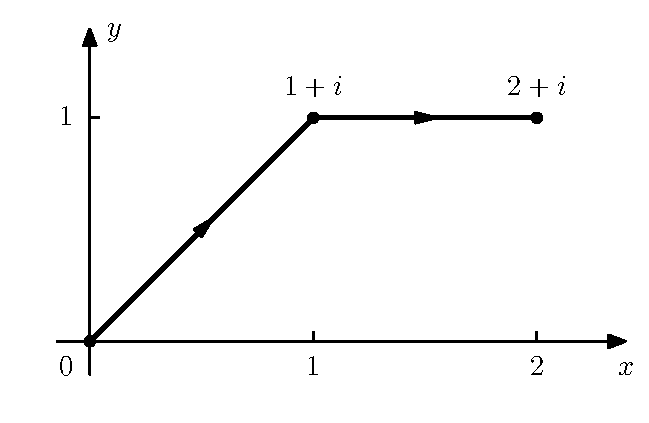
\includegraphics[width=\textwidth]{figuras/example_43_01_polygonal_line_contour.pdf}
  \end{minipage}\hfill
  \begin{minipage}[c]{0.4\textwidth}
    \caption{
       Arco simple.
    }\label{fig:example_43_01_polygonal_line_contour}
  \end{minipage}
\end{figure}

La representación paramétrica de una curva \(C\) dada no es única. De hecho es posible cambiar el intervalo del parámetro por cualquier otro intervalo. Específicamente, supóngase que 
\begin{equation}\label{eq:contours_parameter_transformation}
 t=\phi(\tau),\qquad\qquad\textrm{con}\qquad\qquad\alpha\leq\tau\leq\beta, 
\end{equation}
donde \(\phi\) es una función real que mapea el intervalo \(\alpha\leq\tau\leq\beta\) en el intervalo \(a\leq t\leq b\) en la representación \ref{eq:contours_arc_definition_complex}, como se muestra en la figura \ref{fig:contours_parameter_transformation}. Se asume que \(\phi\) es continua con derivada continua. También se asume que \(\phi'(\tau)>0\) para cada \(\tau\) de forma de asegurar que \(t\) crezca con \(\tau\). De esta forma, la representación \ref{eq:contours_arc_definition_complex} es transformada mediante la ecuación \ref{eq:contours_parameter_transformation} en la representación
\begin{equation}\label{eq:contours_arc_transformation_complex}
 z=Z(\tau),\qquad\qquad\textrm{con}\qquad\qquad\alpha\leq\tau\leq\beta, 
\end{equation}
donde
\[
 Z(\tau)=z[\phi(\tau)].
\]
Esto se ilustra en el ejercicio 3 de esta sección.
\begin{figure}[!htb]
  \begin{minipage}[c]{0.5\textwidth}
    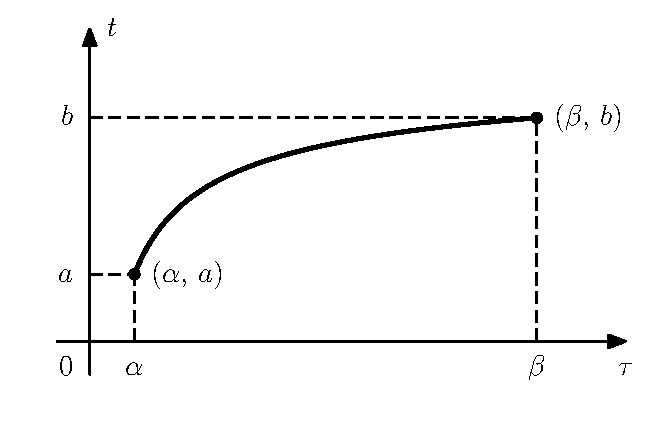
\includegraphics[width=\textwidth]{figuras/contours_parameter_transformation.pdf}
  \end{minipage}\hfill
  \begin{minipage}[c]{0.4\textwidth}
    \caption{
       \(t=\phi(\tau)\).
    }\label{fig:contours_parameter_transformation}
  \end{minipage}
\end{figure}

Supóngase ahora que los componentes \(x'(t)\) y \(y'(t)\) de la derivada 
\[
 z'(t)=x'(t)+iy'(t)
\]
de la función \ref{eq:contours_arc_definition_complex_components} (ver la sección \ref{sec:integrals_derivatives_of_wt}) empleada para representar \(C\) son continuos en todo el intervalo \(a\leq t\leq b\). En ese caso, el arco se llama \emph{arco diferenciable}, y la función real 
\[
 |z'(t)|=\sqrt{[x'(t)]^2+[y'(t)]^2}
\]
es integrable en el intervalo \(a\leq t\leq b\). De hecho, de acuerdo a la definición de longitud de arco en cálculo (ver por ejemplo la sección 10.3 de \cite{larson2009calculus} o la sección 10.2 de \cite{stewart2016essential}), la longitud de \(C\) es el número
\begin{equation}\label{eq:contours_arc_length}
 L=\int_a^b|z'(t)|\,dt. 
\end{equation}

Como es de esperarse, el número \(L\) es invariante ante algunos cambios en la representación de \(C\) usada. Mas precisamente, con el cambio de variable \ref{eq:contours_parameter_transformation}, la ecuación \ref{eq:contours_arc_length} queda (ver el ejercicio 1(\textit{b}) de esta sección)
\[
 L=\int_\alpha^\beta|z'[\phi(\tau)]|\phi'(\tau)\,d\tau.
\]
Por lo tanto, si se emplea la representación \ref{eq:contours_arc_transformation_complex} para \(C\), como la derivada es (ver el ejercicio 4)
\begin{equation}\label{eq:contours_arc_transformation_complex_derivative}
 Z'(\tau)=z'[\phi(\tau)]\phi'(\tau), 
\end{equation}
resulta en que 
\[
 L=\int_\alpha^\beta|Z'(\tau)|\,d\tau.
\]
Esto indica que se obtiene la misma longitud de \(C\) al emplear la representación \ref{eq:contours_arc_transformation_complex}. 

Si la ecuación \ref{eq:contours_arc_definition_complex} representa un arco diferenciable y si \(z'(t)\neq0\) en todo el intervalo \(a<t<b\), el vector tangente unitario
\[
 \T=\frac{z'(t)}{|z'(t)|}
\]
está bien definido para todo \(t\) en dicho intervalo abierto y el ángulo de inclinación es \(\arg z'(t)\). Además, cuando \(\T\) gira lo hace de forma continua a medida que el parámetro \(t\) varía en todo el intervalo \(a<t<b\). La expresión para \(\T\) es la deducida en cálculo cuando \(z(t)\) se interpreta como un radio vector (ver la sección 12.4 de \cite{larson2009calculus}). Un arco con estas características se dice que es \emph{suave} (ver la sección 10.2 de \cite{larson2009calculus}). Por lo tanto, al hacer referencia a un arco suave \(z=z(t),\;a\leq t\leq b\), se entenderá que la derivada \(z'(t)\) es continua en el intervalo cerrado \(a\leq t\leq b\) y no nula en el intervalo abierto \(a<t<b\).

Un \emph{contorno}, o arco suave a trozos, es un arco que consiste en un número finito de arcos suaves unidos por los extremos. De esta forma, si la ecuación \ref{eq:contours_arc_definition_complex} representa un contorno, \(z(t)\) es continua y su derivada \(z'(t)\) es continua a trozos. Cuando solo coinciden el valor inicial y final de \(z(t)\), el contorno \(C\) se llama \emph{contorno cerrado simple}. La longitud de un contorno o un contorno cerrado simple es la suma de las longitudes de los arcos suaves que conforman el contorno.

Los puntos de cualquier curva cerrada simple o contorno cerrado simple son los puntos de la frontera de dos dominios distintos, uno de los cuales es el interior de \(C\) y es acotado, y el otro es el exterior de \(C\) y es no acotado. Esta afirmación, llamada \emph{teorema de la curva de Jordan}, si bien es evidente geométricamente, no es fácil de demostrar.

\subsection*{Ejercicios}

\subsubsection{Ejercicio 1}

Mostrar que si \(w(t)=u(t)+iv(t)\) es continua en el intervalo \(a\leq t\leq b\), entonces
\begin{enumerate}
 \item[(\textit{a})] \(\displaystyle\int_{-b}^{-a}w(-t)\,dt=\int_{a}^{b}w(t)\,dt\);
 \item[(\textit{b})] \(\displaystyle\int_{a}^{b}w(t)\,dt=\int_\alpha^\beta w[\phi(\tau)]\phi'(\tau)\,dt\), donde \(\phi(\tau)\) es la función de la ecuación \ref{eq:contours_parameter_transformation}.
\end{enumerate}

\emph{Sugerencia:} las identidades pueden deducirse observando que son válidas para funciones reales de variable real \(t\).

\paragraph{Solución.} 
\begin{enumerate}
 \item[(\textit{a})] Como \(w(-t)=u(-t)+iv(-t)\), partiendo de la definición \ref{eq:integrals_wt_integral_definition}, se tiene que 
 \begin{align*}
  \int_{-b}^{-a}w(-t)\,dt&=\int_{-b}^{-a}u(-t)\,dt+i\int_{-b}^{-a}v(-t)\,dt\\
    &=-\int_{b}^{a}u(\tau)\,d\tau-i\int_{b}^{a}v(\tau)\,d\tau\\
    &=\int_{a}^{b}u(\tau)\,d\tau+i\int_{a}^{b}v(\tau)\,d\tau\\
    &=\int_{a}^{b}w(t)\,dt,
 \end{align*}
 donde se emplearon propiedades de integrales de una función real de variable real, y en particular, el cambio de variable \(\tau=-t\).
 \item[(\textit{b})] Nuevamente, partiendo de la definición \ref{eq:integrals_wt_integral_definition} se ve que 
 \begin{align*}
  \int_{a}^{b}w(t)\,dt&=\int_{a}^{b}u(t)\,dt+i\int_{a}^{b}v(t)\,dt\\
   &\overset{(a)}{=}\int_{\phi^{-1}(a)}^{\phi^{-1}(b)}u[\phi(\tau)]\phi'(\tau)\,d\tau+i\int_{\phi^{-1}(a)}^{\phi^{-1}(b)}v[\phi(\tau)]\phi'(\tau)\,d\tau\\
   &\overset{(b)}{=}\int_\alpha^\beta u[\phi(\tau)]\phi'(\tau)\,d\tau+i\int_\alpha^\beta v[\phi(t)]\phi'(\tau)\,d\tau\\
   &\overset{(c)}{=}\int_\alpha^\beta\left\{u[\phi(\tau)]\phi'(\tau)+iv[\phi(\tau)]\phi'(\tau)\right\}\,d\tau\\
   &=\int_\alpha^\beta\left\{u[\phi(\tau)]+iv[\phi(\tau)]\right\}\phi'(\tau)\,d\tau\\
   &=\int_\alpha^\beta w[\phi(\tau)]\phi'(\tau)\,d\tau,
 \end{align*}
 donde en \((a)\) se realizó el cambio de variable \(t=\phi(\tau)\) y por lo tanto, \(dt=\phi'(\tau)d\tau\), notando que \(\phi^{-1}(t)\) existe por ser \(\phi(\tau)\) una función monótonamente creciente. Esto puede hacerse por tratarse de integrales de una función real de variable real. En \((b)\) se consideró que \(\phi(\alpha)=a\) y \(\phi(\beta)=b\) y por lo tanto, \(\phi^{-1}(a)=\alpha\) y \(\phi^{-1}(b)=\beta\) y en \((c)\) se empleó nuevamente la definición \ref{eq:contours_parameter_transformation} de la integral de una función compleja de variable real.
\end{enumerate}

\subsubsection{Ejercicio 2}

Sea \(C\) la mitad derecha del círculo \(|z|=2\) en sentido antihorario, y se observa que dos representaciones paramétricas de \(C\) son 
\[
 z=z(\theta)=2e^{i\theta},
 \qquad\qquad\textrm{con}\qquad\qquad
 -\frac{\pi}{2}\leq\theta\leq\frac{\pi}{2} 
\]
y
\[
 z=Z(y)=\sqrt{4-y^2}+iy,
 \qquad\qquad\textrm{con}\qquad\qquad
 -2\leq y\leq2.
\]
Verificar que \(Z(y)=z[\phi(y)]\), donde 
\[
 \phi(y)=\arctan\frac{y}{\sqrt{4-y^2}},
 \qquad\qquad\textrm{con}\qquad\qquad
 -\frac{\pi}{2}\leq\theta\leq\frac{\pi}{2}. 
\]
Además, mostrar que dicha función \(\phi\) tiene derivada positiva, como se requiere. 

\paragraph{Solución.} En la figura \ref{fig:exercise_43_02} se observa que si la parte imaginaria de un punto \(z=2e^{i\theta}\) que pertenece a \(C\) es \(y\), la parte real es \(x=\sqrt{4-y^2}\). Por lo tanto,
\[
 z=z(\theta)=2e^{i\theta},
 \qquad\qquad\textrm{con}\qquad\qquad
 -\frac{\pi}{2}\leq\theta\leq\frac{\pi}{2} 
\]
y
\[
 z=Z(y)=\sqrt{4-y^2}+iy,
 \qquad\qquad\textrm{con}\qquad\qquad
 -2\leq y\leq2
\]
son representaciones equivalentes de \(C\). 
\begin{figure}[!htb]
  \begin{minipage}[c]{0.35\textwidth}
    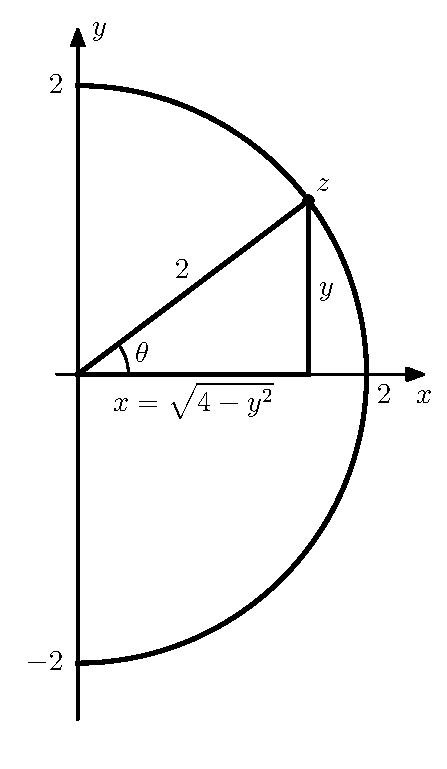
\includegraphics[width=\textwidth]{figuras/exercise_43_02.pdf}
  \end{minipage}\hfill
  \begin{minipage}[c]{0.55\textwidth}
    \caption{
       Arco \(C\) que consiste en la mitad derecha del círculo unidad. Puede parametrizarse como \(z(\theta)=2e^{i\theta}\) con \(-\pi/2\leq\theta\leq\pi/2\) o como \(Z(y)=\sqrt{4-y^2}+iy\) con \(-2\leq y\leq2\).
    }\label{fig:exercise_43_02}
  \end{minipage}
\end{figure}

Se verificará que
\[
 Z(y)=z[\phi(y)]
 \qquad\qquad\textrm{con}\qquad\qquad
 \phi(y)=\arctan\frac{y}{\sqrt{4-y^2}}.
\]
Para hacerlo, se parte observando que 
\begin{align}
 z[\phi(y)]&=2\exp\left(i\arctan\frac{y}{\sqrt{4-y^2}}\right)\nonumber\\ 
  &=2\left[\cos\left(\arctan\frac{y}{\sqrt{4-y^2}}\right)+i\sen\left(\arctan\frac{y}{\sqrt{4-y^2}}\right)\right].\label{eq:exercise_34_02_z_phi}
\end{align}
Del triángulo en la figura \ref{fig:exercise_43_02} se ve que
\[
 \tan\theta=\frac{y}{\sqrt{4-y^2}}
 \qquad\qquad\textrm{o}\qquad\qquad
 \theta=\arctan\frac{y}{\sqrt{4-y^2}}.
\]
Además,
\[
 \cos\theta=\frac{\sqrt{4-y^2}}{2}
 \qquad\qquad\textrm{o}\qquad\qquad
 \cos\left(\arctan\frac{y}{\sqrt{4-y^2}}\right)=\frac{\sqrt{4-y^2}}{2}
\]
y
\[
 \sen\theta=\frac{y}{2}
 \qquad\qquad\textrm{o}\qquad\qquad
 \sen\left(\arctan\frac{y}{\sqrt{4-y^2}}\right)=\frac{y}{2}.
\]
Sustituyendo estos resultados en la ecuación \ref{eq:exercise_34_02_z_phi} se obtiene que 
\[
 z[\phi(y)]=2\left(\frac{\sqrt{4-y^2}}{2}+\frac{iy}{2}\right)
 =\sqrt{4-y^2}+iy=Z(y),
\]
que es lo que se quería mostrar.

Se mostrará que la función \(\phi\) tiene derivada positiva. Para eso, considerando que \(\arctan'x=1/(1+x^2)\), se tiene que 
\begin{align*}
 \phi'(y)&=\dfrac{1}{1+\left(\dfrac{y}{\sqrt{4-y^2}}\right)^2}\times
  \frac{\sqrt{4-y^2}-y\dfrac{1}{2}(4-y^2)^{-1/2}(-2y)}{4-y^2}\\
  &=\dfrac{1}{1+\dfrac{y^2}{4-y^2}}\times\dfrac{\sqrt{4-y^2}+\dfrac{y^2}{\sqrt{4-y^2}}}{4-y^2}\\
  &=\frac{1}{4-y^2+y^2}\times\frac{4-y^2+y^2}{\sqrt{4-y^2}},
\end{align*}
concluyendo que 
\[
 \phi'(y)=\frac{1}{\sqrt{4-y^2}}>0
 \qquad\qquad\textrm{en}\qquad\qquad
 -2<y<2.
\]

\subsubsection{Ejercicio 3}

Deducir la ecuación de la recta que pasa por los puntos \((\alpha,\,a)\) y \((\beta,\,b)\) en el plano \(\tau t\) de la figura \ref{fig:contours_parameter_transformation}. Luego, emplearla para encontrar la función lineal \(\phi(\tau)\) que puede emplearse en la ecuación \ref{eq:contours_parameter_transformation} para transformar la representación \ref{eq:contours_arc_definition_complex} en la representación \ref{eq:contours_arc_transformation_complex}

\paragraph{Solución.} La ecuación de la recta que pasa por los puntos \((\alpha,\,a)\) y \((\beta,\,b)\) en el plano \(\tau t\) es
\[
 t-a=\frac{b-a}{\beta-\alpha}(\tau-\alpha),
\]
y operando se ve que
\begin{align*}
 t&=\frac{b-a}{\beta-\alpha}\tau-\frac{b-a}{\beta-\alpha}\alpha+a\\
  &=\frac{b-a}{\beta-\alpha}\tau-\frac{a(\beta-\alpha)-(b-a)\alpha}{\beta-\alpha}\\
  &=\frac{b-a}{\beta-\alpha}\tau-\frac{a\beta-b\alpha}{\beta-\alpha}.
\end{align*}
Por lo tanto, la función lineal \(\phi(\tau)\) que cambia el intervalo del parámetro de \([a,\,b]\) a \([\alpha,\,\beta]\) es
\[
 \phi(\tau)=\frac{b-a}{\beta-\alpha}\tau-\frac{a\beta-b\alpha}{\beta-\alpha}.
\]

\subsubsection{Ejercicio 4}

Deducir la ecuación \ref{eq:contours_arc_transformation_complex_derivative} de la derivada de \(Z(\tau)=z[\phi(\tau)]\).

\emph{Sugerencia:} escribir \(Z(\tau)=x[\phi(\tau)]+iy[\phi(\tau)]\) y aplicar la regla de la cadena para funciones reales de variable real.

\paragraph{Solución.} Con \(z(t)=x(t)+iy(t)\), se tiene que 
\[
 Z(\tau)=z[\phi(\tau)]=x[\phi(\tau)]+iy[\phi(\tau)].
\]
Por lo tanto, de la definición \ref{eq:derivatives_wt_derivative_definition} y aplicando la regla de la cadena para funciones reales de variable real,
\begin{align*}
 Z'(\tau)&=\frac{dx[\phi(\tau)]}{d\tau}+i\frac{dy[\phi(\tau)]}{d\tau}\\
 &=x'[\phi(\tau)]\phi'(\tau)+iy'[\phi(\tau)]\phi'(\tau)\\
 &=\left\{x'[\phi(\tau)]+iy'[\phi(\tau)]\right\}\phi'(\tau)\\
 &=z'[\phi(\tau)]\phi'(\tau).
\end{align*}

\subsubsection{Ejercicio 5}

Supóngase que una función \(f(z)\) es analítica en un punto \(z_0=z(t_0)\) que pertenece a un arco suave \(z=z(t)\), \(a\leq t\leq b\). Mostrar que si \(w(t)=f[z(t)]\), se cumple que 
\[
 w'(t)=f'[z(t)]z'(t)
\]
cuando \(t=t_0\).

\emph{Sugerencia:} escribir \(f(z)=u(x,\,y)+iv(x,\,y)\) y \(z(t)=x(t)+iy(t)\) de forma que 
\[
 w(t)=u[x(t),\,y(t)]+iv[x(t),\,y(t)].
\]
Luego, aplicar la regla de la cadena de cálculo para funciones reales de dos variables reales para obtener que 
\[
 w'(t)=(u_xx'+u_yy')+i(v_xx'+v_yy'),
\]
y finalmente emplear las ecuaciones de Cauchy-Riemann.

\paragraph{Solución.} Aplicando la definición \ref{eq:derivatives_wt_derivative_definition} de la derivada y siguiendo los pasos indicados en la sugerencia, se obtiene que 
\[
 w'(t)=(u_xx'+u_yy')+i(v_xx'+v_yy').
\]
Como \(f(z)\) es analítica en \(z_0=z(t_0)\), se cumplen las ecuaciones 
\[
 u_x=v_y
 \qquad\qquad\textrm{y}\qquad\qquad
 v_x=-u_y
\]
de Cauchy-Riemann en \(t=t_0\), que pueden emplearse para expresar \(w'(t)\) solo en función de las derivadas respecto a \(x\),
\begin{align*}
 w'(t)&=(u_xx'-v_xy')+i(v_xx'+u_xy')\\
  &\overset{(a)}{=}(u_x+iv_x)x'+(u_x+iv_x)iy'\\
  &=(u_x+iv_x)(x'+iy')\\
  &\overset{(b)}{=}f'[z(t)]z'(t),
\end{align*}
donde en \((a)\) se consideró que el término \(-v_xy'\) puede escribirse como \(iiv_xy'\) y en \((b)\) se emplearon las ecuaciones \ref{eq:cauchy_riemann_f_derivative} y \ref{eq:derivatives_wt_derivative_definition}.

\subsubsection{Ejercicio 6}

Sea \(y(x)\) una función real definida en el intervalo \(0\leq x\leq1\) como
\[
 y(x)=\left\{ 
 \begin{array}{ll}
  x^3\sen(\pi/x)&\textrm{cuando }0<x\leq1\\
  0&\textrm{cuando }x=0.
 \end{array}
 \right.
\]
\begin{enumerate}
 \item[(\textit{a})] Mostrar que la ecuación
 \[
  z=x+iy(x),
  \qquad\qquad\textrm{con}\qquad\qquad
  0\leq x\leq1,
 \]
 representa un arco \(C\) que intersecta el eje real en los puntos \(z=1/n\), \(n=1,\,2,\,\dots\) y \(z=0\), como se muestra en la figura \ref{fig:exercise_43_06}.
 \begin{figure}[!htb]
  \begin{minipage}[c]{0.56\textwidth}
    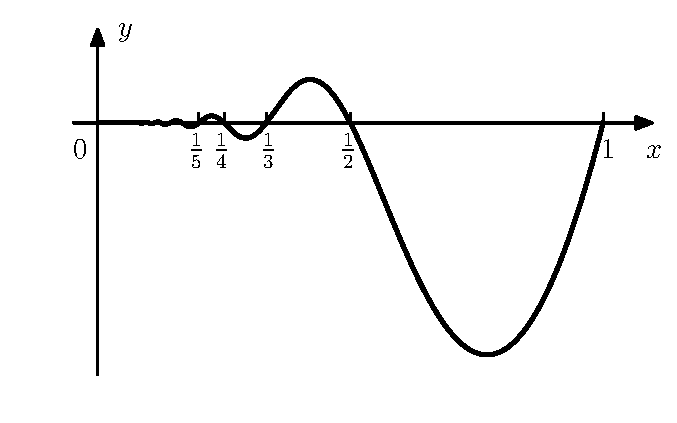
\includegraphics[width=\textwidth]{figuras/exercise_43_06.pdf}
  \end{minipage}\hfill
  \begin{minipage}[c]{0.34\textwidth}
    \caption{
       Arco \(z=x+iy(x)\).
    }\label{fig:exercise_43_06}
  \end{minipage}
\end{figure}
 \item[(\textit{b})] Verificar que el arco \(C\) de la parte (\textit{a}) es de hecho un arco suave.
 \end{enumerate}
 
\emph{Sugerencia:} Para establecer la continuidad de \(y(x)\) en \(x=0\), observar que 
\[
 0\leq\left|x^3\sen\left(\frac{\pi}{x}\right)\right|\leq x^3
\]
cuando \(x>0\). Una observación similar puede emplearse para encontrar \(y'(0)\) y mostrar que \(y'(x)\) es continua en \(x=0\).

\paragraph{Solución.} 
\begin{enumerate}
 \item[(\textit{a})] \(z(x)=x+iy(x)\) es un arco en \(0\leq x\leq1\) si sus componentes real e imaginario son continuos en dicho intervalo. El componente real \(x\) es obviamente continuo con \(x\). Es fácil ver que el componente imaginario \(y(x)\) es continuo en el intervalo \(0<x\leq1\), pero falta ver si es continuo en \(x=0\), para lo cual se debe cumplir que 
\[
 \lim_{x\to0^+}y(x)=y(0).
\]
En este caso, la condición de continuidad es
\begin{equation}\label{eq:exersice_43_06_z_continuity_condition}
  \lim_{x\to0^+}x^3\sen\left(\frac{\pi}{x}\right)=0.
\end{equation}
Observando que si \(x>0\), se cumple que 
\[
 0\leq\left|x^3\sen\left(\frac{\pi}{x}\right)\right|\leq x^3,
\]
tomado el límite, 
\[
 0\leq\lim_{x\to0^+}\left|x^3\sen\left(\frac{\pi}{x}\right)\right|\leq\lim_{x\to0^+}x^3=0,
\]
concluyendo que efectivamente se cumple la condición de continuidad \ref{eq:exersice_43_06_z_continuity_condition}, y por lo tanto, \(z(x)\) es un arco.

El arco \(C\) intersecta al eje real en los valores en donde la parte imaginaria de \(z\) se anula, es decir, en los valores \(x\) tales que \(y(x)=0\). Por un lado, en el intervalo \(0<x\leq1\),
\[
 y(x)=x^3\sen\left(\frac{\pi}{x}\right)=0
 \quad\Leftrightarrow\quad 
 \sen\left(\frac{\pi}{x}\right)=0
 \quad\Leftrightarrow\quad 
 \frac{\pi}{x}=n\pi
 \quad\Leftrightarrow\quad
 x=\frac{1}{n},
 \quad
 n=1,\,2,\,\dots.
\]
Además, en \(x=0\), \(y(x)=0\). Se concluye que el arco \(C\) corta al eje real en los puntos \(z=1/n\), \(n=1,\,2,\,\dots\), y en \(z=0\).
\item[(\textit{b})] \(C\) es un arco suave si se cumple que \(z'(x)\) es continua en \(0\leq x\leq1\) y no nula en \(0<x<1\). Derivando respecto a \(x\), se tiene que
\[
 z'(x)=1+iy'(x),
 \qquad\qquad\textrm{con}\qquad\qquad
 0\leq x\leq1.
\]
\(y(x)\) es continua, como se mostró en la parte (\textit{a}) y como está definida a trozos, la derivada en el intervalo \(0<x\leq1\) es 
\[
 y'(x)=3x^2\sen\left(\frac{\pi}{x}\right)+x^3\left(-\frac{\pi}{x}\right)\cos\left(\frac{\pi}{x}\right)=3x^2\sen\left(\frac{\pi}{x}\right)-\pi x\cos\left(\frac{\pi}{x}\right).
\]
En \(x=0\), la derivada puede calcularse empleando su definición,
\[
 y'(0)=\lim_{x\to0^+}\frac{y(x)-y(0)}{x-0}=\lim_{x\to0^+}\frac{y(x)}{x}
\]
y es
\[
 y'(0)=\lim_{x\to0^+}x^2\sen\left(\frac{\pi}{x}\right)=0,
\]
donde la última igualdad se obtiene empleando el mismo argumento que en el estudio de la continuidad de \(y(x)\) en \(x=0\) en la parte (\textit{a}). Se obtuvo que 
\[
 y'(x)=\left\{ 
 \begin{array}{ll}
  3x^2\sen\left(\dfrac{\pi}{x}\right)-\pi x\cos\left(\dfrac{\pi}{x}\right)&\textrm{en }0<x\leq1\\
  0&\textrm{en }x=0.
 \end{array}
 \right.
\]
Como con \(x>0\) se cumple que 
\[
 0\leq\left|3x^2\sen\left(\dfrac{\pi}{x}\right)-\pi x\cos\left(\dfrac{\pi}{x}\right)\right|
 \leq\left|3x^2\sen\left(\dfrac{\pi}{x}\right)\right|+\left|\pi x\cos\left(\dfrac{\pi}{x}\right)\right|\leq3x^2+\pi x\xrightarrow[x\to0^+]{} 0
\]
se obtiene que 
\[
 \lim_{x\to0^+}y'(x)=\lim_{x\to0^+}\left[3x^2\sen\left(\dfrac{\pi}{x}\right)-\pi x\cos\left(\dfrac{\pi}{x}\right)\right]=0=y'(0),
\]
concluyendo que \(y'(x)\) es continua en el intervalo \(0\leq x\leq1\), y por lo tanto, \(z'(x)\) es continua en el intervalo \(0\leq x\leq1\).

Por otro lado, como la parte real de \(z(x)\) es 1 para todo \(x\) en el intervalo \(0\leq x\leq1\), \(z'(x)\) es no nula en dicho intervalo, concluyendo que se trata de un arco suave.
\end{enumerate}

\section{Integrales de contorno}\label{sec:contour_integrals}

Se pasa ahora al estudio de integrales de funciones complejas de variable compleja \(z\). Dichas integrales se definen en términos de los valores de \(f(z)\) sobre un contorno \(C\) dado que se extiende desde el punto \(z=z_1\) al punto \(z=z_2\) en el plano complejo. Es por lo tanto una integral de línea, y su valor depende en general del contorno \(C\) así como de la función \(f\). Se denota como
\[
 \int_{C}f(z)\,dz
 \qquad\qquad\textrm{o}\qquad\qquad
 \int_{z_1}^{z_2}f(z)\,dz,
\]
donde la segunda notación se emplea cuando la integral es independiente del contorno elegido entre los puntos fijos de los extremos. Si bien la integral puede definirse como el límite de una suma, se elige aquí la definición en términos de la integral definida de la ecuación \ref{eq:integrals_wt_integral_definition}.

Sea
\[
 z=z(t),\qquad\qquad\textrm{con}\qquad\qquad a\leq t\leq b, 
\]
un contorno \(C\) que se extiende desde el punto \(z_1=z(a)\) hasta el punto \(z_2=z(b)\). Se asume que \(f[z(t)]\) es continua a trozos (ver la sección \ref{sec:definite_integrals_wt}) en el intervalo \(a\leq t\leq b\) y se dice que la función \(f(z)\) es continua a trozos en \(C\). Luego, se define la integral de línea o \emph{integral de contorno} de \(f\) sobre \(C\) en términos del parámetro \(t\):
\begin{equation}\label{eq:contour_integral_definition}
 \int_C f(z)\,dz=\int_a^b f[z(t)]z'(t)\,dz.
\end{equation}
Observar que como \(C\) es un contorno, \(z'(t)\) es continua a trozos en \(a\leq t\leq b\) (ver la sección \ref{sec:contours}), por lo que está asegurada la existencia de la integral \ref{eq:contour_integral_definition}. 

El valor de una integral de contorno es invariante ante cambios en la representación del contorno cuando el cambio es del tipo \ref{eq:contours_arc_transformation_complex}

A continuación se mencionan algunas propiedades de las integrales de contorno. Se comienza aceptando que dado un contorno \(C\) dado, \(-C\) denota el mismo conjunto de puntos pero en orden reverso. Observar que si \(C\) tiene la representación \ref{eq:contours_arc_definition_complex}, una representación para \(-C\) es
\begin{equation}\label{eq:contours_reverse_contour}
 z=z(-t),\qquad\qquad\textrm{con}\qquad\qquad -b\leq t\leq-a. 
\end{equation}

Si \(C_1\) es un contorno desde \(z_1\) hasta \(z_2\) y \(C_2\) es un contorno desde \(z_2\) hasta \(z_3\) el contorno resultante es la \emph{suma} y se denota \(C=C_1+C_2\). Observar que la suma de los contornos \(C_1\) y \(-C_2\) está bien definida cuando \(C_1\) y \(C_2\) tienen el mismo punto final, y se denota \(C=C_1-C_2\).

En los enunciados de las propiedades de las integrales de contorno se asume que todas las funciones \(f(z)\) y \(g(z)\) son continuas a trozos sobre cualquier contorno empleado.

Si \(z_0\) es una constante compleja se cumple que 
\[
 \int_C z_0f(z)\,dz= z_0\int_C f(z)\,dz.
\]
También es cierto que 
\[
 \int_C[f(z)+g(z)]\,dz=\int_C f(z)\,dz+\int_C g(z)\,dz
\]
Ambas propiedades se obtienen a partir de la definición \ref{eq:continuity_definition} y las propiedades de las integrales de funciones complejas \(w(t)\) con variable real vistas en la sección \ref{sec:definite_integrals_wt}. Además, empleando la representación \ref{eq:contours_reverse_contour} y los resultados del ejercicio 1(\textit{b}) de la sección \ref{sec:definite_integrals_wt} y del ejercicio ejercicio 1(\textit{a}) de la sección \ref{sec:contours} puede probarse que 
\[
 \int_{-C}f(z)\,dz= -\int_C f(z)\,dz.
\]
También puede deducirse que si \(C=C_1+C_2\), se cumple que
\[
 \int_{C}f(z)\,dz=\int_{C_1}f(z)\,dz+\int_{C_2}f(z)\,dz.
\]

\section{Algunos ejemplos}\label{sec:contour_integrals_examples}

El objetivo de esta sección y la siguiente es mostrar como se evalúan las integrales de contorno empleando la definición \ref{eq:contour_integral_definition} así como ilustrar el uso de algunas de las propiedades mencionadas en la sección \ref{sec:contour_integrals}. El desarrollo de primitivas se aplaza para la sección \ref{sec:antiderivatives}.

\paragraph{Ejemplo 1} Se calculará la integral de contorno
\[
 \int_{C_1}\frac{dz}{z}
\]
donde \(C_1\) es la mitad superior
\[
 z=e^{i\theta},\qquad\qquad\textrm{con}\qquad\qquad 0\leq\theta\leq\pi, 
\]
del círculo \(|z|=1\) desde \(z=1\) hasta \(z=-1\), como se muestra en la figura \ref{fig:example_45_01}. De acuerdo a la definición \ref{eq:contour_integral_definition}
\begin{equation}\label{eq:example_45_01_integral_c1}
 \int_{C_1}\frac{dz}{z}=\int_0^\pi\frac{1}{e^{i\theta}}ie^{i\theta}\,d\theta=i\int_0^\pi\,d\theta=\pi i. 
\end{equation}
\begin{figure}[!htb]
  \begin{minipage}[c]{0.35\textwidth}
    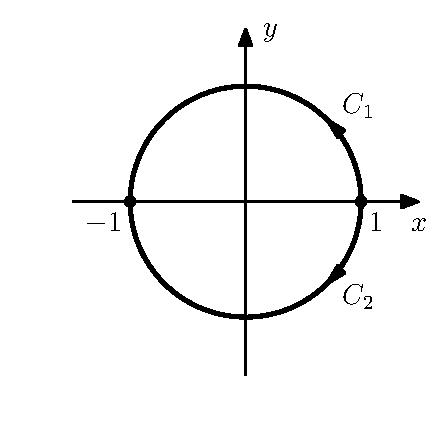
\includegraphics[width=\textwidth]{figuras/example_45_01.pdf}
  \end{minipage}\hfill
  \begin{minipage}[c]{0.55\textwidth}
    \caption{
        Contornos \(C_1\) y \(C_2\) empleados en el ejemplo 1.
    }\label{fig:example_45_01}
  \end{minipage}
\end{figure}

Se considera ahora la integral
\[
 \int_{C_2}\frac{dz}{z}.
\]
sobre la mitad inferior del mismo círculo \(|z|=1\) desde \(z=1\) hasta \(z=-1\), también mostrado en la figura \ref{fig:example_45_01}. Para evaluar esta integral, se empleará la representación paramétrica  
\[
 z=e^{i\theta},\qquad\qquad\textrm{con}\qquad\qquad \pi\leq\theta\leq2\pi, 
\]
del contorno \(-C_2\). Por lo tanto,
\begin{equation}\label{eq:example_45_01_integral_c2}
 \int_{C_2}\frac{dz}{z}=-\int_{-C_2}\frac{dz}{z}=-\int_\pi^{2\pi}\frac{1}{e^{i\theta}}ie^{i\theta}\,d\theta=-i\int_\pi^{2\pi}\,d\theta=-\pi i. 
\end{equation}

Observar que los valores de las integrales \ref{eq:example_45_01_integral_c1} y \ref{eq:example_45_01_integral_c2} difieren a pesar de que los extremos de los contornos \(C_1\) y \(C_2\) son los mismos. Notar también que si \(C\) es la curva cerrada \(C=C_1-C_2\),
\[
 \int_C\frac{dz}{z}=\int_{C_1}\frac{dz}{z}-\int_{C_2}\frac{dz}{z}=\pi i-(-\pi i)=2\pi i.
\]

\paragraph{Ejemplo 2} Sea \(C\) un arco suave arbitrario
\[
 z=z(t),\qquad\qquad\textrm{con}\qquad\qquad a\leq t\leq b,
\]
desde el punto fijo \(z_1\) hasta el punto fijo \(z_2\), y se quiere evaluar la integral
\[
 \int_C z\,dz=\int_a^bz(t)z'(t)\,dt.
\]
A partir de las consideraciones de la sección \ref{sec:integrals_derivatives_of_wt} puede probarse que se cumple que 
\[
 \frac{d}{dt}\frac{[z(t)]^2}{2}=z(t)z'(t)
\]
y por lo tanto
\[
 \int_C z\,dz=\frac{[z(t)]^2}{2}\bigg|_a^b=\frac{[z(b)]^2-[z(a)]^2}{2}=\frac{z_2^2-z_1^2}{2},
\]
donde se consideró que \(z(a)=z_1\) y \(z(b)=z_2\). Se observa que el valor de esta integral depende únicamente de los puntos extremos de \(C\) y por lo tanto, es independiente del arco específico entre esos puntos, y se puede escribir como
\[
 \int_{z_1}^{z_2}z\,dz=\frac{z_2^2-z_1^2}{2}.
\]

Estos ejemplos ilustran los siguientes importantes hechos sobre integrales de contorno:
\begin{enumerate}
 \item[(\textit{a})] el valor de una integral de contorno de una función dada desde un punto fijo hasta otro puede ser independiente del camino tomado (ejemplo 2), pero no siempre es el caso (ejemplo 1).
 \item[(\textit{b})] las integrales de contorno de una función dada puede ser nula en todo contorno cerrado (ejemplo 2), pero no siempre es el caso (ejemplo 1).
\end{enumerate}

La respuesta a la pregunta de cuando las integrales de contorno son independientes del camino tomado o tienen valor nulo en cada contorno cerrado se responderá en las secciones \ref{sec:antiderivatives}, \ref{sec:cauchy_goursat_theorem} y \ref{sec:simply_connected_domains}. 

\section{Ejemplos que involucran cortes de rama}\label{sec:integrals_examples_with_branch_cuts}

El camino empleado en una integral de contorno puede contener un punto de un corte de rama. Esto se ilustra en el siguiente ejemplo.

\paragraph{Ejemplo} Sea \(C\) el semicírculo superior 
\[
 z=3e^{i\theta},
 \qquad\qquad\textrm{con}\qquad\qquad 0\leq\theta\leq\pi,
\]
desde el punto \(z=3\) hasta el punto \(z=-3\), como se muestra en la figura \ref{fig:example_46_01}. 
\begin{figure}[!htb]
  \begin{minipage}[c]{0.35\textwidth}
    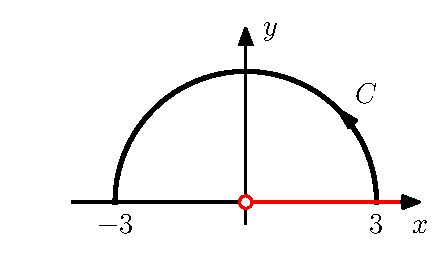
\includegraphics[width=\textwidth]{figuras/example_46_01.pdf}
  \end{minipage}\hfill
  \begin{minipage}[c]{0.55\textwidth}
    \caption{
        Contorno \(C\) y corte de rama de la función \(f(z)\).
    }\label{fig:example_46_01}
  \end{minipage}
\end{figure}
A pesar de que la rama
\[
 f(z)=z^{1/2}=\exp\left(\frac{1}{2}\log z\right),
 \qquad\qquad
 |z|>0,\,0<\arg z<2\pi
\]
de la función multivaluada \(z^{1/2}\) (ver la sección \ref{sec:power_function}) no está definida en el punto inicial \(z=3\) del contorno \(C\) (ver la figura \ref{fig:example_46_01}), la integral 
\[
 I=\int_C z^{1/2}\,dz
\]
existe, ya que el integrando es continuo a trozos en \(C\) (ver la sección \ref{sec:definite_integrals_wt}). Para ver esto, se observa primero que cuando \(z(\theta)=3e^{i\theta}\),
\begin{align*}
 f[z(\theta)]&\overset{(a)}{=}\exp\left[\frac{1}{2}\log(3e^{i\theta})\right]\\
  &\overset{(b)}{=}\exp\left[\frac{1}{2}(\ln 3+i\theta)\right]\\
  &=\exp\left(\ln\sqrt{3}+\frac{i\theta}{2}\right)\\
  &=\sqrt{3}e^{i\theta/2},
\end{align*}
donde en \((a)\) se aplicó la definición \ref{eq:power_function} de la función potencia y en \((b)\) la definición \ref{eq:logarithm_definition_branch} de una rama de la función logarítmica. Luego, considerando que \(z'(\theta)=3ie^{i\theta}\),
\[
 f[z(\theta)]z'(\theta)=\sqrt{3}e^{i\theta/2}3ie^{i\theta}=3\sqrt{3}ie^{i3\theta/2}
 =3\sqrt{3}i\left(\cos\frac{3\theta}{2}+i\sen\frac{3\theta}{2}\right),
 \qquad\qquad 0<\theta\leq\pi,
\]
resultando en que 
\[
 f[z(\theta)]z'(\theta)=-3\sqrt{3}\sen\frac{3\theta}{2}+i3\sqrt{3}\cos\frac{3\theta}{2},
 \qquad\qquad 0<\theta\leq\pi.
\]
Se observa que los límites cuando \(\theta\to0^+\) de los componentes real e imaginario de \(f[z(\theta)]z'(\theta)\) existen y son respectivamente \(0\) y \(3\sqrt{3}\). Esto implica que la función \(f[z(\theta)]z'(\theta)\) es continua en el intervalo cerrado \(0\leq\theta\leq\pi\) cuando su valor en \(\theta=0\) se define como \(i3\sqrt{3}\). Continuando,
\[
 I=3\sqrt{3}i\int_0^\pi e^{i3\theta/2}\,d\theta
 =3\sqrt{3}i\left(\frac{2}{i3}e^{i3\theta/2}\bigg|_0^\pi\right)
 =2\sqrt{3}\left(e^{i3\pi/2}-1\right),
\]
y como \(e^{i3\pi/2}=-i\) resulta en que 
\[
 I=-2\sqrt{3}(1+i).
\]


\subsection*{Ejercicios}

Para las funciones \(f\) y contornos \(C\) en los ejercicios del 1 al 8, emplear representaciones paramétricas de \(C\) para evaluar
\[
 \int_C f(z)\,dz.
\]

\subsubsection{Ejercicio 1}

\(f(z)=(z+2)/z\) y \(C\) es
\begin{itemize}
 \item[(\textit{a})] el semicírculo \(z=2e^{i\theta}\) con \(0\leq\theta\leq\pi\);
 \item[(\textit{b})] el semicírculo \(z=2e^{i\theta}\) con \(\pi\leq\theta\leq2\pi\);
 \item[(\textit{c})] el círculo \(z=2e^{i\theta}\) con \(0\leq\theta\leq2\pi\).
\end{itemize}

\paragraph{Solución}

\begin{itemize}
 \item[(\textit{a})] Con  \(z(\theta)=2e^{i\theta}\),
 \[
  f[z(\theta)]z'(\theta)=\frac{2e^{i\theta}+2}{2e^{i\theta}}2ie^{i\theta}=2i(e^{i\theta}+1).
 \]
 Por lo tanto,
 \begin{align*}
  \int_C\frac{z+2}{z}\,dz&=2i\int_0^\pi(e^{i\theta}+1)\,d\theta\\
   &=2i\left[\left(\frac{1}{i}e^{i\theta}+\theta\right)\bigg|_0^\pi\right]\\
   &=2i\left[\left(\frac{1}{i}e^{i\pi}+\pi\right)-\left(\frac{1}{i}\right)\right]\\
   &=2i\left(-\frac{1}{i}+\pi-\frac{1}{i}\right)\\
   &=2\left(-2+\pi i\right)\\
   &=-4+2\pi i.
 \end{align*}
 \item[(\textit{b})] De forma similar,
 \begin{align*}
  \int_C\frac{z+2}{z}\,dz&=2i\int_\pi^{2\pi}(e^{i\theta}+1)\,d\theta\\
   &=2i\left[\left(\frac{1}{i}e^{i\theta}+\theta\right)\bigg|_\pi^{2\pi}\right]\\
   &=2i\left[\left(\frac{1}{i}e^{i2\pi}+2\pi\right)-\left(\frac{1}{i}e^{i\pi}+\pi\right)\right]\\
   &=2i\left[\left(\frac{1}{i}+2\pi\right)-\left(-\frac{1}{i}+\pi\right)\right]\\
   &=2i\left(\frac{2}{i}+\pi\right)\\
   &=4+2\pi i.
 \end{align*}
 \item[(\textit{c})] Con \(C_1\) el contorno \(z=2e^{i\theta}\) con \(0\leq\theta\leq\pi\) de la parte (\textit{a}) y \(C_2\) el contorno \(z=2e^{i\theta}\) con \(\pi\leq\theta\leq2\pi\) de la parte (\textit{b}), se cumple que \(C=C_1+C_2\), como se muestra en la figura \ref{fig:exercise_46_01}. Por lo tanto,
 \[
  \int_C\frac{z+2}{z}\,dz=\int_{C_1}\frac{z+2}{z}\,dz+\int_{C_2}\frac{z+2}{z}\,dz
  =(-4+2\pi i)+(4+2\pi i)=4\pi i.
 \]
 \begin{figure}[!htb]
  \begin{minipage}[c]{0.35\textwidth}
    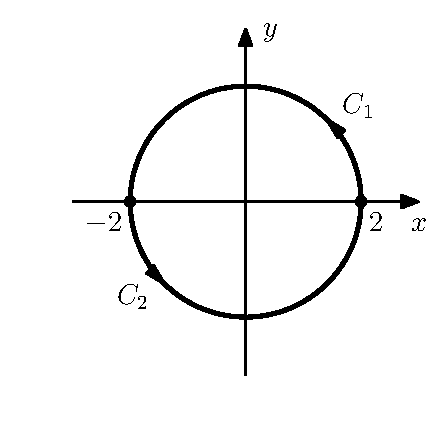
\includegraphics[width=\textwidth]{figuras/exercise_46_01.pdf}
  \end{minipage}\hfill
  \begin{minipage}[c]{0.55\textwidth}
    \caption{
        Contornos empleados en el ejercicio 1. Si \(C_1\) es el contorno de la parte (\textit{a}) y \(C_2\) es el contorno de la parte (\textit{b}), el contorno de la parte (\textit{c}), que es el círculo completo, es \(C=C_1+C_2\).
    }\label{fig:exercise_46_01}
  \end{minipage}
\end{figure}
\end{itemize}

\subsubsection{Ejercicio 2}

\(f(z)=z-1\) y \(C\) es el arco desde \(z=0\) a \(z=2\) que consiste en
\begin{itemize}
 \item[(\textit{a})] el semicírculo \(z=1+e^{i\theta}\) con \(\pi\leq\theta\leq2\pi\);
 \item[(\textit{b})] el segmento \(z=x\) con \(0\leq x\leq2\) del eje real.
\end{itemize}

\paragraph{Solución.} 
\begin{itemize}
 \item[(\textit{a})] El contorno \(z=1+e^{i\theta}\) con \(\pi\leq\theta\leq2\pi\) es el semicírculo mostrado en la figura \ref{fig:exercise_46_02}.
En este caso, 
\[
 f[z(\theta)]z'(\theta)=\left[(1+e^{i\theta})-1\right]ie^{i\theta}=ie^{i2\theta},
 \qquad\qquad
 \pi\leq\theta\leq2\pi.
\]
 \begin{figure}[!htb]
  \begin{minipage}[c]{0.35\textwidth}
    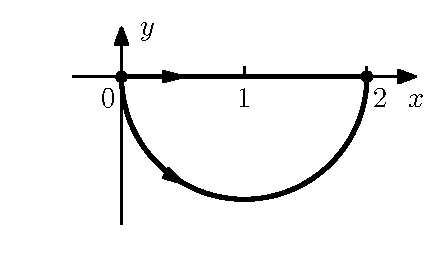
\includegraphics[width=\textwidth]{figuras/exercise_46_02.pdf}
  \end{minipage}\hfill
  \begin{minipage}[c]{0.55\textwidth}
    \caption{
        Contornos empleados en el ejercicio 2.
    }\label{fig:exercise_46_02}
  \end{minipage}
\end{figure}
Por lo tanto,
\begin{align*}
 \int_C(z-1)\,dz=i\int_\pi^{2\pi}e^{i2\theta}\,d\theta=i\frac{e^{i2\theta}}{2i}\bigg|_\pi^{2\pi}=\frac{1}{2}(e^{i4\pi}-e^{i2\pi})=\frac{1}{2}(1-1)=0.
\end{align*}
 \item[(\textit{b})] Con el contorno \(z=x\) con \(0\leq x\leq2\) en eje real (ver la figura \ref{fig:exercise_46_02}),
 \[
  f[z(x)]z'(x)=(x-1)\times1=x-1,
  \qquad\qquad
 0\leq x\leq2.
 \]
 Por lo tanto,
 \[
  \int_C(z-1)\,dz=i\int_0^2(x-1)\,dx=\left(\frac{x^2}{2}-x\right)\bigg|_0^2=(2-2)-(0-0)=0.
 \]
\end{itemize}

\subsubsection{Ejercicio 3}

\(f(z)=\exp(\pi\overline{z})\) y \(C\) es la frontera de cuadrado con vértices en los puntos \(0\), \(1\), \(1+i\) y \(i\) y la orientación de \(C\) es en sentido antihorario.

\paragraph{Solución.} Se comienza calculando la integral sobre los contornos \(C_1\), \(C_2\), \(C_3\) y \(C_4\) mostrados en la figura \ref{fig:exercise_46_03}.
 \begin{figure}[!htb]
  \begin{minipage}[c]{0.32\textwidth}
    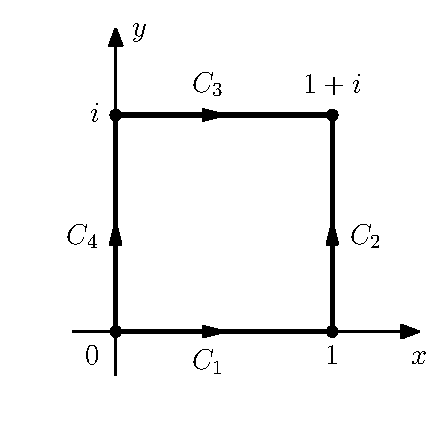
\includegraphics[width=\textwidth]{figuras/exercise_46_03.pdf}
  \end{minipage}\hfill
  \begin{minipage}[c]{0.58\textwidth}
    \caption{
       Contornos empleados en el ejercicio 3.
    }\label{fig:exercise_46_03}
  \end{minipage}
 \end{figure}

En el contorno \(C_1\) del eje real entre los puntos \(z=0\) y \(z=1\), \(z=x\) con \(0\leq x\leq1\), se tiene que 
\[
 f[z(x)]z'(x)=\pi e^{\pi x},
\]
y por lo tanto,
\[
 \int_{C_1}e^{\pi\overline{z}}\,dz=\pi\int_0^1e^{\pi x}\,dx=\pi\frac{e^{\pi x}}{\pi}\bigg|_0^1=e^\pi-1.
\]
En el contorno \(C_2\) entre los puntos \(z=1\) y \(z=1+i\), \(z=1+iy\) con \(0\leq y\leq1\), se tiene que 
\[
 f[z(x)]z'(x)=\pi e^{\pi(1-iy)}i,
\]
y por lo tanto,
\[
 \int_{C_2}e^{\pi\overline{z}}\,dz=i\pi e^\pi\int_0^1e^{-i\pi y}\,dy=i\pi e^\pi\frac{e^{-i\pi y}}{-i\pi}\bigg|_0^1=-e^\pi(e^{-i\pi}-1)=-e^\pi(-1-1)=2e^\pi.
\]
En el contorno \(C_3\) entre los puntos \(z=1+i\) y \(z=i\), \(z=x+i\) con \(0\leq x\leq1\), se tiene que 
\[
 f[z(x)]z'(x)=\pi e^{\pi(x-i)},
\]
y por lo tanto,
\[
 \int_{C_3}e^{\pi\overline{z}}\,dz=\pi e^{-\pi i}\int_0^1e^{\pi x}\,dx=\pi e^{-\pi i}\frac{e^{\pi x}}{\pi}\bigg|_0^1=-(e^\pi-1).
\]
En el contorno \(C_4\) entre los puntos \(z=i\) y \(z=0\), \(z=iy\) con \(0\leq y\leq1\), se tiene que 
\[
 f[z(x)]z'(x)=\pi e^{-i\pi y}i,
\]
y por lo tanto,
\[
 \int_{C_4}e^{\pi\overline{z}}\,dz=i\pi\int_0^1e^{-i\pi y}\,dy=i\pi\frac{e^{-i\pi y}}{-i\pi}\bigg|_0^1=-(e^{-i\pi}-1)=-(-1-1)=2.
\]
Luego, considerando que \(C=C_1+C_2-C_3-C_4\), se obtiene que 
\begin{align*}
 \int_{C}e^{\pi\overline{z}}\,dz&=\int_{C_1+C_2-C_3-C_4}e^{\pi\overline{z}}\,dz\\
  &=\int_{C_1}e^{\pi\overline{z}}\,dz+\int_{C_2}e^{\pi\overline{z}}\,dz+\int_{-C_3}e^{\pi\overline{z}}\,dz+\int_{-C_4}e^{\pi\overline{z}}\,dz\\
  &=\int_{C_1}e^{\pi\overline{z}}\,dz+\int_{C_2}e^{\pi\overline{z}}\,dz-\int_{C_3}e^{\pi\overline{z}}\,dz-\int_{C_4}e^{\pi\overline{z}}\,dz\\
  &=(e^\pi-1)+2e^\pi+(e^\pi-1)-2\\
  &=4(e^\pi-1).
\end{align*}

\subsubsection{Ejercicio 4}

\(f(z)\) definida como
\[
 f(z)=\left\{ 
 \begin{array}{ll}
  1 & \textrm{si }y<0\\
  4y & \textrm{si }y>0,
 \end{array}
 \right.
\]
y \(C\) es el arco desde \(z=-1-i\) hasta \(z=1+i\) por la curva \(y=x^3\).

\paragraph{Solución.} El arco \(C\) se puede parameterizar como 
\[
 z=x+ix^3,
 \qquad\qquad
 -1\leq x\leq1,
\]
y como con \(y=x^3\) se cumple que \(x<0\) si y solo si \(y<0\) y \(x>0\) si y solo si \(y>0\),
\[
 f[z(x)]=\left\{ 
 \begin{array}{ll}
  1 & \textrm{si }-1\leq x\leq 0\\[\smallskipamount]
  4x^3 & \textrm{si }0\leq x\leq 1.
 \end{array}
 \right.
\]
Además, como \(z'(x)=1+i3x^2\),
\[
 f[z(x)]z'(x)=\left\{ 
 \begin{array}{ll}
  1+i3x^2 & \textrm{si }-1\leq x\leq0\\[\smallskipamount]
  4x^3(1+i3x^2) & \textrm{si }0\leq x\leq 1.
 \end{array}
 \right.
\]
\begin{figure}[!htb]
  \begin{minipage}[c]{0.35\textwidth}
    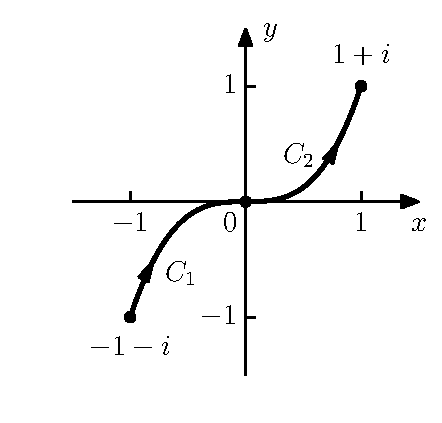
\includegraphics[width=\textwidth]{figuras/exercise_46_04.pdf}
  \end{minipage}\hfill
  \begin{minipage}[c]{0.55\textwidth}
    \caption{
        Contornos \(C_1\) y \(C_2\) empleados en el ejercicio 4.
    }\label{fig:exercise_46_04}
  \end{minipage}
\end{figure}
Por lo tanto, con \(C_1:\,z=x+ix^3\) con \(-1\leq x\leq0\) (ver la figura \ref{fig:exercise_46_04}),
\[
 \int_{C_1}f(z)\,dz=\int_{-1}^{0}f[z(x)]z'(x)\,dx=\int_{-1}^{0}(1+i3x^2)\,dx=(x+ix^3)\bigg|_{-1}^{0}=0-(-1-i)=1+i
\]
y con \(C_2:\,z=x+ix^3\) con \(0\leq x\leq1\),
\begin{align*}
 \int_{C_2}f(z)\,dz&=\int_{0}^{1}f[z(x)]z'(x)\,dx\\
   &=\int_{0}^{1}4x^3(1+i3x^2)\,dx\\ 
   &=4\int_{0}^{1}x^3\,dx+12i\int_{0}^{1}x^5\,dx\\
   &=4\frac{x^4}{4}\bigg|_{0}^{1}+12i\frac{x^6}{6}\bigg|_{0}^{1}\\
   &=x^4\bigg|_{0}^{1}+2ix^6\bigg|_{0}^{1}\\
   &=1+2i.
\end{align*}
Finalmente,
\[
 \int_C f(z)\,dz=\int_{C_1}f(z)\,dz+\int_{C_2}f(z)\,dz=(1+i)+(1+2i)=2+3i.
\]

\subsubsection{Ejercicio 5}

\(f(z)=1\) y \(C\) es un contorno arbitrario desde algún punto fijo \(z_1\) hasta otro punto fijo \(z_2\).

\paragraph{Solución.} Sea \(z=z(t)\) con \(a\leq t\leq b\) alguna parametrización del contorno \(C\), donde \(z(a)=z_1\) y \(z(b)=z_2\). De esta forma,
\[
 \int_Cf(z)\,dz=\int_a^bf[z(t)]z'(t)\,dt=\int_a^b1\times z'(t)\,dt=z(t)\bigg|_a^b=z(b)-z(a)=z_2-z_1.
\]

\subsubsection{Ejercicio 6}

\(f(z)\) es la rama principal de
\[
 z^i=\exp(i\Log z),
 \qquad\qquad
 |z|>0,\,-\pi<\Arg z<\pi
\]
de la función potencia \(z^i\), y \(C\) es el semicírculo \(z=e^{i\theta}\) con \(0\leq\theta\leq\pi\).

\paragraph{Solución.} 
\[
 f[z(\theta)]=\exp\left(i\Log e^{i\theta}\right)=\exp\left[i(\ln1+i\theta)\right]=e^{-\theta},
 \qquad\qquad
 0\leq\theta<\pi,
\]
y
\[
 f[z(\theta)]z'(t)=e^{-\theta}ie^{i\theta},
 \qquad\qquad
 0\leq\theta<\pi.
\]
Observar que como
\[
 f[z(\theta)]z'(t)=e^{-\theta}i(\cos\theta+i\sen\theta)=-e^{-\theta}\sen\theta+ie^{-\theta}\cos\theta
\]
y por lo tanto,
\[
 \lim_{\theta\to\pi^-}f[z(\theta)]z'(t)=-e^{-\pi}\sen\pi+ie^{-\pi}\cos\pi=-ie^{-\pi}
\]
por lo que \(f[z(\theta)]z'(t)\) es continua en el intervalo cerrado \(0\leq\theta\leq\pi\) si se define \(f[z(\theta)]z'(t)=-ie^{-\pi}\) en \(\theta=\pi\), asegurando la existencia de la integral. Continuando,
\[
 \int_Cz^i\,dz=i\int_0^\pi e^{(-1+i)\theta}\,d\theta=i\frac{e^{(-1+i)\theta}}{-1+i}\bigg|_0^\pi
  =\frac{i}{-1+i}\left[e^{(-1+i)\pi}-1\right]=\frac{i(-1-i)}{2}\left(e^{-\pi}e^{-i\pi}-1\right),
\]
resultando en que 
\[
 \int_Cz^i\,dz=-\frac{e^{-\pi}+1}{2}(1-i).
\]

\subsubsection{Ejercicio 7}

\(f(z)\) es la rama principal de
\[
 z^{-1-2i}=\exp\left[(-1-2i)\Log z\right],
 \qquad\qquad
 |z|>0,\,-\pi<\Arg z<\pi
\]
de la función potencia indicada, y \(C\) es el contorno
\[
 z=e^{i\theta},
 \qquad\qquad
 0\leq\theta\leq\frac{\pi}{2}.
\]

\paragraph{Solución.} 
\[
 f[z(\theta)]=\exp\left[(-1-2i)\Log e^{i\theta}\right]=\exp\left[(-1-2i)(\ln1+i\theta)\right]=\exp(2\theta-i\theta)=e^{(2-i)\theta}.
\]
y
\[
 f[z(\theta)]z'(\theta)=e^{(2-i)\theta}ie^{i\theta}=ie^{2\theta},
 \qquad\qquad
 0\leq\theta\leq\frac{\pi}{2}.
\]
Por lo tanto,
\[
 \int_Cz^{-1-2i}\,d\theta=i\int_0^{\pi/2}e^{2\theta}\,d\theta=i\frac{e^{2\theta}}{2}\bigg|_0^{\pi/2}=i\frac{e^\pi-1}{2}.
\]

\subsubsection{Ejercicio 8}

\(f(z)\) es la rama principal de
\[
 z^{a-1}=\exp\left[(a-1)\Log z\right],
 \qquad\qquad
 |z|>0,\,-\pi<\Arg z<\pi
\]
de la función potencia \(z^{a-1}\), donde \(a\) es un número real no nulo, y \(C\) es el círculo de radio \(R\) centrado en el origen orientado positivamente.

\paragraph{Solución.} El contorno \(C\) es
\[
 z=Re^{i\theta},
 \qquad\qquad
 R>0,\,-\pi\leq\theta\leq\pi.
\]
De esta forma,
\[
 f[z(\theta)]=\exp\left[(a-1)\Log(Re^{i\theta})\right]=\exp\left[(a-1)(\ln R+i\theta)\right]
  =\exp\left[\ln R^{a-1}+i(a-1)\theta\right]=R^{a-1}e^{i(a-1)\theta}
\]
y
\begin{equation}\label{eq:exercise_46_08_integrand}
  f[z(\theta)]z'(\theta)=R^{a-1}e^{i(a-1)\theta}Rie^{i\theta}=iR^ae^{ia\theta},
 \qquad\qquad
 -\pi<\theta<\pi.
\end{equation}
Por lo tanto,
\[
 \int_C z^{a-1}\,dz=iR^a\int_{-\pi}^{\pi}e^{ia\theta}\,d\theta=iR^a\frac{e^{ia\theta}}{ia}\bigg|_{-\pi}^{\pi}
  =\frac{iR^a}{a}\left(\frac{e^{ia\pi}-e^{-ia\pi}}{i}\right)
\]
resultando en que 
\[
 \int_C z^{a-1}\,dz=\frac{2iR^a}{a}\sen(a\pi).
\]

\subsubsection{Ejercicio 9}

Sea \(C\) el círculo unidad centrado en el origen \(|z|=1\) orientado positivamente.
\begin{enumerate}
 \item[(\textit{a})] Mostrar que si \(f(z)\) es la rama principal
 \[
  z^{-3/4}=\exp\left(-\frac{3}{4}\Log z\right),
 \qquad\qquad
 |z|>0,\,-\pi<\Arg z<\pi
 \]
 de \(z^{-3/4}\), se cumple que 
 \[
  \int_Cf(z)\,dz=4\sqrt{2}i.
 \]
 \item[(\textit{b})] Mostrar que si \(g(z)\) es la rama
 \[
  z^{-3/4}=\exp\left(-\frac{3}{4}\log z\right),
 \qquad\qquad
 |z|>0,\,0<\arg z<2\pi
 \]
 de la misma función potencia de la parte (\textit{a}), se cumple que 
 \[
  \int_Cg(z)\,dz=-4+4i.
 \]
 Este ejercicio muestra como el valor de la integral de una función potencia depende en general de la rama empleada.
\end{enumerate}

\paragraph{Solución}
\begin{enumerate}
 \item[(\textit{a})] En este caso, \(C\) es \(z=e^{i\theta}\) con \(-\pi<\theta<\pi\). Por lo tanto
 \[
  f[z(\theta)]=\exp\left(-\frac{3}{4}\Log e^{i\theta}\right)=\exp\left[-\frac{3}{4}(\ln1+i\theta)\right]=e^{-i3\theta/4},
 \]
 y
 \[
  f[z(\theta)]z'(\theta)=e^{-i3\theta/4}ie^{i\theta}=ie^{i\theta/4}.
 \]
 Luego,
 \[
  \int_Cf(z)\,dz=i\int_{-\pi}^\pi e^{i\theta/4}\,d\theta=i\frac{e^{i\theta/4}}{i/4}\bigg|_{-\pi}^\pi=4(e^{i\pi/4}-e^{i\pi/4})=4\left(2i\sen\frac{\pi}{4}\right)=4\left(2i\frac{\sqrt{2}}{2}\right)=4\sqrt{2}i.
 \]
 \item[(\textit{b})] Ahora, el contorno \(C\) se parametriza como \(z=e^{i\theta}\) con \(0\leq\theta\leq2\pi\). Por lo tanto, 
 \[
  \int_Cg(z)\,dz=i\int_0^{2\pi}e^{i\theta/4}\,d\theta=4e^{i\theta/4}\bigg|_0^{2\pi}=4(e^{i\pi/2}-1)=4(i-1)=-4+4i.
 \]
\end{enumerate}

\subsubsection{Ejercicio 10}

Con la ayuda del resultado del ejercicio 3 de la sección \ref{sec:definite_integrals_wt}, evaluar la integral 
\[
 \int_Cz^m\overline{z}^n\,dz,
\]
donde \(m\) y \(n\) son enteros y \(C\) es el círculo unidad \(|z|=1\) en sentido antihorario.

\paragraph{Solución.} Sea el contorno \(C\) parametrizado como \(z=e^{i\theta}\) con \(0\leq\theta\leq2\pi\). De esta forma, con \(f(z)=z^m\overline{z}^n\) donde \(m\) y \(n\) son enteros,
\[
 f[z(t\theta)]z'(\theta)=e^{im\theta}e^{-in\theta}ie^{i\theta}=ie^{i(m+1)\theta}e^{-in\theta}.
\]
Por lo tanto,
\[
 \int_Cf(z)\,dz=i\int_0^{2\pi}e^{i(m+1)\theta}e^{-in\theta}\,d\theta=
 \left\{ 
 \begin{array}{ll}
  0 & \textrm{si }m+1\neq n\\
  2\pi i & \textrm{si }m+1=n,
 \end{array}
 \right.
\]
donde en la última igualdad se empleó el resultado del ejercicio 3 de la sección \ref{sec:definite_integrals_wt}.

\subsubsection{Ejercicio 11}

Sea \(C\) el contorno semicircular mostrado en la figura \ref{fig:exercise_46_11}. 
\begin{figure}[!htb]
 \begin{minipage}[c]{0.24\textwidth}
  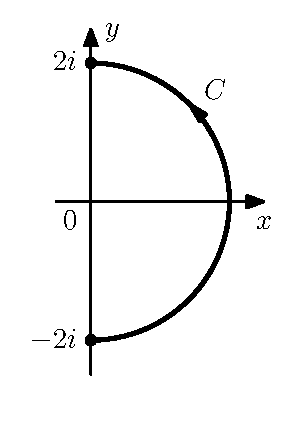
\includegraphics[width=\textwidth]{figuras/exercise_46_11.pdf}
 \end{minipage}\hfill
 \begin{minipage}[c]{0.66\textwidth}
  \caption{
    Contorno empleado en el ejercicio 11.
    }\label{fig:exercise_46_11}
 \end{minipage}
\end{figure}
Evaluar la integral de la función \(f(z)=\overline{z}\) sobre \(C\) empleando la representación paramétrica (ver el ejercicio 2 de la sección \ref{sec:contours})
\[
 (\textit{a})\;z=2e^{i\theta},\qquad-\frac{\pi}{2}\leq\theta\leq\frac{\pi}{2};\qquad\qquad (\textit{b})\;z=\sqrt{4-y^2}+iy,\qquad-2\leq y\leq2.
\]

\paragraph{Solución.} 
\begin{enumerate}
 \item[(\textit{a})] En este caso,
 \[
  f[z(\theta)]z'(\theta)=2e^{-i\theta}2ie^{i\theta}=4i,
 \]
 y por lo tanto,
 \[
  \int_C\overline{z}\,dz=4i\int_{-\pi/2}^{\pi/2}\,d\theta=4i\theta\bigg|_{-\pi/2}^{\pi/2}
  =4i\left[\frac{\pi}{2}-\left(-\frac{\pi}{2}\right)\right]=4\pi i.
 \]
 \item[(\textit{b})] Como se vio en el ejercicio 2 de la sección \ref{sec:contours},
 \[
  z=\sqrt{4-y^2}+iy,
  \qquad\qquad-2\leq y\leq2,
 \]
 es una representación paramétrica de \(C\). Como
 \[
  z'(y)=\frac{1}{2}(4-y^2)^{-1/2}(-2y)+i=-\frac{y}{\sqrt{4-y^2}}+i,
 \]
 se tiene que 
 \begin{align*}
  f[z(y)]z'(y)&=\left(\sqrt{4-y^2}-iy\right)\left(-\frac{y}{\sqrt{4-y^2}}+i\right)\\
    &=-y+y+i\left(\sqrt{4-y^2}+\frac{y^2}{\sqrt{4-y^2}}\right)\\
    &=i\frac{4-y^2+y^2}{\sqrt{4-y^2}}\\
    &=\frac{4i}{\sqrt{4-y^2}}.
 \end{align*}
 Por lo tanto,
 \begin{align*}
  \int_C\overline{z}\,dz&=4i\int_{-2}^2\frac{1}{\sqrt{4-y^2}}\,dy\\
   &\overset{(a)}{=}\arcsen\left(\frac{y}{2}\right)\bigg|_{-2}^2\\
   &=4i[\arcsen(1)-\arcsen(-1)]\\
   &=4i\left[\frac{\pi}{2}-\left(-\frac{\pi}{2}\right)\right]\\
   &=4\pi i,
 \end{align*}
donde en \((a)\) se tuvo en cuenta que\footnote{Ver \url{https://en.wikipedia.org/wiki/Differentiation_of_trigonometric_functions}, por ejemplo.} 
\[
 \frac{d}{dx}\arcsen\left(\frac{x}{a}\right)=\frac{1}{\sqrt{a^2-x^2}}.
\]
\end{enumerate}

\subsubsection{Ejercicio 12}

\begin{enumerate}
 \item[(\textit{a})] Supóngase que una función \(f(z)\) es continua en un arco suave \(C\) con representación paramétrica \(z=z(t)\) con \(a\leq t\leq b\); es decir, \(f[z(t)]\) es continua en el intervalo \(a\leq t\leq b\). Mostrar que si \(\phi(\tau)\) con \(\alpha\leq\tau\leq\beta\) es la función descripta en la sección \ref{sec:contours}, se cumple que 
 \[
  \int_a^bf[z(t)]z'(t)\,dt=\int_\alpha^\beta f[Z(\tau)]Z'(\tau)\,d\tau,
 \]
 donde \(Z(\tau)=z[\phi(\tau)]\).
 \item[(\textit{b})] Indicar porque el resultado obtenido en la parte (\textit{a}) continúa siendo válido cuando \(C\) es cualquier contorno, y no necesariamente uno suave, y \(f(z)\) es continua a trozos en \(C\). De esta forma, mostrar que el valor de la integral de \(f(z)\) sobre \(C\) es igual cuando se emplea la representación \(z=Z(\tau)\) con \(\alpha\leq\tau\leq\beta\) en lugar de la representación original.
\end{enumerate}

\emph{Sugerencia:} en la parte (\textit{a}) emplear el resultado del ejercicio 1(\textit{b}) de la sección \ref{sec:contours} y referirse a la ecuación \ref{eq:contours_arc_transformation_complex_derivative}.

\paragraph{Solución.} 

\begin{enumerate}
 \item[(\textit{a})] Se observa que 
 \begin{align*}
  \int_a^bf[z(t)]z'(t)\,dt&\overset{(a)}{=}\int_\alpha^\beta f[Z(\tau)]z'[\phi(\tau)]\phi'(\tau)\,d\tau\\
   &\overset{(b)}{=}\int_\alpha^\beta f[Z(\tau)]Z'(\tau)\,d\tau,
 \end{align*}
 donde en \((a)\) se realizó el cambio de variable \(t=\phi(\tau)\) y se empleó el resultado del ejercicio 1(\textit{b}) de la sección \ref{sec:contours}, que indica que con dicho cambio de variable,
 \[
  \int_{a}^{b}w(t)\,dt=\int_\alpha^\beta w[\phi(\tau)]\phi'(\tau)\,d\tau,
 \]
 donde en este caso, \(w(t)=f[z(t)]z'(t)\) y por lo tanto \(w[\phi(\tau)]=f[Z(\tau)]z'[\phi(\tau)]\) y se definió \(Z(\tau)=z[\phi(\tau)]\), y en \((b)\) se tuvo en cuenta que \(Z'(\tau)=z'[\phi(\tau)]\phi'(\tau)\) (ver la ecuación \ref{eq:contours_arc_transformation_complex_derivative}).
 \item[(\textit{b})] Si \(C\) es un contorno cualquiera y \(f(z)\) es continua a trozos sobre \(C\), \(C\) puede partirse en una cantidad finita de arcos suaves sobre cada uno de los cuales \(f(z)\) es continua. Por lo tanto, el resultado de la parte (\textit{a}) sigue siendo válido.
\end{enumerate}

\subsubsection{Ejercicio 13}

Sea \(C_0\) el círculo de centro \(z_0\) y radio \(R\). Emplear la parametrización 
\[
 z=z_0+Re^{i\theta},
 \qquad\qquad
 -\pi\leq\theta\leq\pi.
\]
para mostrar que 
\[
 \int_{C_0}(z-z_0)^{n-1}\,dz=
 \left\{ 
 \begin{array}{ll}
  0 &\textrm{si }n=\pm1,\,\pm2,\,\dots\\
  2\pi i&\textrm{si }n=0.
 \end{array}
 \right.
\]

\paragraph{Solución.} Sea \(f(z)=(z-z_0)^{n-1}\). De la definición de la función potencia, 
\[
 f(z)=(z-z_0)^{n-1}=\exp\left[(n-1)\log(z-z_0)\right].
\]
Notar que como el exponente es entero, \(f(z)\) no es multivaluada, por lo que no es necesario especificar una rama (ver por ejemplo, el ejercicio 6 de la sección \ref{sec:power_function}). Sobre \(C_0\), \(z-z_0=Re^{i\theta}\), y por lo tanto
\[
 f[z(\theta)]=\exp\left[(n-1)\log(Re^{i\theta})\right]=\exp\left[(n-1)(\ln R+i\theta)\right]
  =R^{n-1}e^{i(n-1)\theta},
 \qquad\qquad
 -\pi\leq\theta\leq\pi. 
\]
Además,
\[
 f[z(\theta)]z'(\theta)=R^{n-1}e^{i(n-1)\theta}Rie^{i\theta}=iR^ne^{in\theta},
 \qquad\qquad
 -\pi\leq\theta\leq\pi. 
\]
Por lo tanto,
\[
 \int_{C_0}(z-z_0)^{n-1}\,dz=iR^n\int_{-\pi}^{\pi}e^{in\theta}\,d\theta=\frac{2iR^n}{n}\sen(n\pi),
\]
donde en la última igualdad se empleó el resultado del ejercicio 8 con \(a=n\), ya que las integrales obtenidas en ambos ejercicios son idénticas. Aplicando la regla de l'Hôpital (ver el ejercicio 4 de la sección \ref{sec:differentiation_rules}), se observa que 
\[
 \frac{\sen(n\pi)}{n}=
 \left\{ 
 \begin{array}{ll}
  0 &\textrm{si }n=\pm1,\,\pm2,\,\dots\\
  \pi&\textrm{si }n=0,
 \end{array}
 \right.
\]
resultando en que 
\[
 \int_{C_0}(z-z_0)^{n-1}\,dz=
 \left\{ 
 \begin{array}{ll}
  0 &\textrm{si }n=\pm1,\,\pm2,\,\dots\\
  2\pi i&\textrm{si }n=0.
 \end{array}
 \right.
\]

\section{Cotas superiores para el módulo de integrales de contorno}\label{sec:upper_bounds_for_moduli_of_contour_integrals}

En esta sección se presenta una inecuación que involucra integrales de contorno y es importante en diversas aplicaciones. El resultado se presenta como un teorema y es precedido por un lema basado en funciones del tipo introducido en las secciones \ref{sec:integrals_derivatives_of_wt} y \ref{sec:definite_integrals_wt}

\paragraph{Lema} Si \(w(t)\) es una función compleja continua a trozos definida en un intervalo \(a\leq t\leq b\), se cumple que 
\begin{equation}\label{eq:integrals_wt_tringular_inequality}
 \left|\int_a^b w(t)\,dt\right|\leq\int_a^b|w(t)|\,dt.
\end{equation}

Es claro que la desigualdad se cumple en el caso en que la integral de la izquierda es nula, ya que la integral de la derecha es no negativa por ser el integrando no negativo en todo el intervalo. Por lo tanto, para verificar el resultado se asume que el valor de la integral de la derecha es el número complejo no nulo
\[
 \int_a^b w(t)\,dt=r_0e^{i\theta_0}.
\]
Resolviendo para \(r_0\) resulta en
\[
 r_0=\int_a^b e^{-i\theta_0}w(t)\,dt.
\]
Como el lado izquierdo de la igualdad es un número real, también debe serlo el lado derecho. Por lo tanto, considerando el hecho de que la parte real de un número real es el número mismo, se cumple que 
\[
 r_0=\Re\int_a^b e^{-i\theta_0}w(t)\,dt.
\]
y de la ecuación \ref{eq:integrals_wt_integral_real_imaginary_parts}, se obtiene que 
\[
 r_0=\int_a^b\Re[e^{-i\theta_0}w(t)]\,dt.
\]
Pero como
\[
 \Re[e^{-i\theta_0}w(t)]\leq|e^{-i\theta_0}w(t)|=|e^{-i\theta_0}||w(t)|=|w(t)|
\]
se obtiene que 
\[
 r_0\leq\int_a^b|w(t)|\,dt.
\]
y observando que el lado izquierdo de esta desigualdad es el lado izquierdo de la desigualdad \ref{eq:integrals_wt_tringular_inequality}, se concluye la prueba del lema.

\paragraph{Teorema} Sea \(C\) un contorno de largo \(L\), y sea \(f(z)\) una función continua a trozos sobre \(C\). Si \(M\) es una constante no negativa tal que 
\begin{equation}\label{eq:contour_integral_upper_bound_function_bound}
 |f(z)|\leq M 
\end{equation}
para todos los puntos \(z\) en \(C\) en los cuales \(f(z)\) está definida, se cumple que
\begin{equation}\label{eq:contour_integral_upper_bound}
 \left|\int_{C}f(z)\,dz\right|\leq ML.
\end{equation}

Para obtener la desigualdad \ref{eq:contour_integral_upper_bound}, se parte asumiendo que se cumple la desigualdad \ref{eq:contour_integral_upper_bound_function_bound}, y sea 
\[
 z=z(t),\qquad\qquad\textrm{con}\qquad\qquad a\leq t\leq b,
\]
una representación paramétrica de \(C\). De acuerdo al lema,
\[
 \left|\int_{C}f(z)\,dz\right|=\left|\int_a^bf[z(t)]z'(t)\,dt\right|\leq\int_a^b|f[z(t)]z'(t)|\,dt.
\]
Como
\[
 |f[z(t)]z'(t)|=|f[z(t)]||z'(t)|\leq M|z'(t)|
\]
cuando \(a\leq t\leq b\), excepto posiblemente para un número finito de puntos, se obtiene que 
\[
 \left|\int_{C}f(z)\,dz\right|\leq M\int_a^b|z'(t)|\,dt.
\]
Teniendo en cuenta que, como indica la ecuación \ref{eq:contours_arc_length}, la integral del lado derecho de la desigualdad es la longitud \(L\) de \(C\), se concluye la prueba. Observar que la desigualdad es estricta si la desigualdad \ref{eq:contour_integral_upper_bound_function_bound} es estricta.

Notar que como \(C\) es un contorno y \(f\) es continua a trozos sobre \(C\), siempre existe un número \(M\) como el de la desigualdad \ref{eq:contour_integral_upper_bound_function_bound}. Esto se debe a que la función real \(|f[z(t)]|\) es continua en el intervalo cerrado y acotado \(a\leq t\leq b\) cuando \(f\) es continua sobre \(C\), y una función como esa siempre alcanza un máximo \(M\) en dicho intervalo, como indica el teorema de los valores extremos o teorema de Weierstrass.\footnote{Ver \url{https://en.wikipedia.org/wiki/Extreme_value_theorem} o la sección 4.1 de \cite{stewart2016essential}.} Por lo tanto, \(|f(z)|\) siempre tiene un valor máximo en \(C\) si \(f\) es continua en \(C\). Lo mismo también es cierto cuando \(f\) es continua a trozos en \(C\).

\subsection*{Ejercicios}

\subsubsection{Ejercicio 1}

Sin evaluar la integral, mostrar que 
\[
 (\textit{a})\;\left|\int_C\frac{z+4}{z^3-1}\,dz\right|\geq\frac{6\pi}{7};\qquad\qquad (\textit{b})\;\left|\int_C\frac{1}{z^2-1}\,dz\right|\geq\frac{\pi}{3}
\]
cuando \(C\) es el arco del círculo \(|z|=2\) desde \(z=2\) hasta \(z=2i\) en el primer cuadrante que se muestra en la figura \ref{fig:exercise_47_01}.
\begin{figure}[!htb]
 \begin{minipage}[c]{0.24\textwidth}
  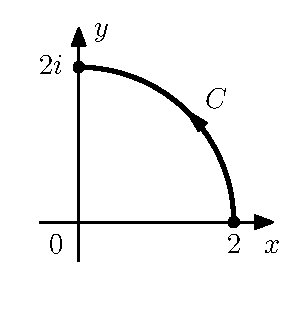
\includegraphics[width=\textwidth]{figuras/exercise_47_01.pdf}
 \end{minipage}\hfill
 \begin{minipage}[c]{0.66\textwidth}
  \caption{
    Contorno empleado en el ejercicio 1.
    }\label{fig:exercise_47_01}
 \end{minipage}
\end{figure}

\paragraph{Solución.} 

Para resolver el problema se empleará la desigualdad \ref{eq:contour_integral_upper_bound}. La longitud del contorno \(C\), que es un cuarto del perímetro de una circunferencia de radio 2, es
\[
 L=\frac{2\pi r}{4}=\frac{4\pi}{4}=\pi,
\]
o a partir de la ecuación \ref{eq:contours_arc_length} considerando que 
\[
 z=2e^{i\theta},
 \qquad\qquad 
 0\leq\theta\leq\frac{\pi}{2},
\]
y por lo tanto,
\[
 z'(\theta)=2ie^{i\theta}
 \qquad\qquad\Rightarrow\qquad\qquad 
 |z'(\theta)|=2,
 \qquad\qquad 
 0\leq\theta\leq\frac{\pi}{2},
\]
resultando en que 
\[
 L=2\int_0^{\pi/2}\,d\theta=2\theta\bigg|_0^{\pi/2}=2\left(\frac{\pi}{2}-0\right)=\pi.
\]
\begin{enumerate}
 \item[(\textit{a})] El uso de la ecuación \ref{eq:contour_integral_upper_bound} requiere encontrar una cota del modulo del integrando en el contorno de integración. Considerando que el módulo del numerador del integrando cumple que
 \[
  |z+4|\leq|z|+|4|=2+4=6,
 \]
 donde se tuvo en cuenta que en el contorno \(C\), \(|z|=2\), y además que el módulo del denominador del integrando cumple que
 \[
  |z^3-1|\geq||z|^3-|1||=|2^3-1|=7,
 \]
 se tiene que 
 \[
  \left|\frac{z+4}{z^3-1}\right|=\frac{|z+4|}{|z^3-1|}\leq\frac{6}{7}.
 \]
 en los puntos \(z\) en \(C\). Se concluye que 
 \[
  \left|\int_C\frac{z+4}{z^3-1}\,dz\right|\leq\frac{6\pi}{7}.
 \]
 \item[(\textit{b})] Como
 \[
  |z^2-1|\geq||z|^2-|1||=|2^2-1|=3,
 \]
 y por lo tanto, el los puntos \(z\) en \(C\), se cumple que 
 \[
  \left|\frac{1}{z^2-1}\right|=\frac{1}{|z^2-1|}\leq\frac{1}{3}.
 \]
 Se concluye que 
 \[
  \left|\int_C\frac{1}{z^2-1}\,dz\right|\geq\frac{\pi}{3}.
 \]
\end{enumerate}

\subsubsection{Ejercicio 2}
 
Sea \(C\) el segmento de recta desde \(z=i\) hasta \(z=1\) que se muestra en la figura \ref{fig:exercise_47_02}. Probar que 
\[
 \left|\int_C\frac{dz}{z^4}\right|\leq4\sqrt{2}
\]
sin evaluar la integral.
\begin{figure}[!htb]
 \begin{minipage}[c]{0.35\textwidth}
   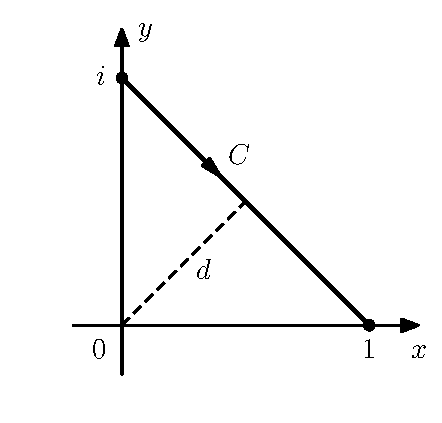
\includegraphics[width=\textwidth]{figuras/exercise_47_02.pdf}
 \end{minipage}\hfill
 \begin{minipage}[c]{0.55\textwidth}
  \caption{
       Contorno empleado en el ejercicio 2.
  }\label{fig:exercise_47_02}
 \end{minipage}
\end{figure}

\emph{Sugerencia:} Observar que de todos los puntos del segmento, el mas cercano al origen es el punto medio, y está a una distancia \(d=\sqrt{2}/2\).

\paragraph{Solución.} Se parte observando que el largo del contorno \(C\) es (ver la figura \ref{fig:exercise_47_02})
\[
 L=\sqrt{2}.
\]
Como el triángulo de vértices en \(0\), \(1\) y \(i\) es isósceles, la mediana y la mediatriz de la hipotenusa coinciden. Por lo tanto, el punto mas cercano al origen del contorno es el punto medio, y como el triángulo formado por los vértices \(0\), \(1\) y el punto medio también es isósceles, la distancia del punto medio del contorno al origen es \(d=L/2=\sqrt{2}/2\). Esto indica que para todo \(z\) en el contorno, se cumple que 
\[
 |z|\geq\frac{\sqrt{2}}{2}.
\]
Teniendo esto en cuenta, el módulo de integrando cumple que 
\[
 \frac{1}{|z^4|}=\frac{1}{|z|^4}\leq\frac{1}{(\sqrt{2}/2)^2}=4.
\]
De la ecuación \ref{eq:contour_integral_upper_bound}, se concluye que 
\[
 \left|\int_C\frac{dz}{z^4}\right|\leq4\sqrt{2}.
\]

\subsubsection{Ejercicio 3}

Mostrar que si \(C\) es la frontera del triángulo con vértices en los puntos \(0\), \(3i\) y \(-4\) orientado en sentido antihorario que se muestra en la figura \ref{fig:exercise_47_03}, se cumple que 
\[
 \left|\int_{C}(e^z-\overline{z})\,dz\right|\leq60.
\]
\begin{figure}[!htb]
 \begin{minipage}[c]{0.35\textwidth}
   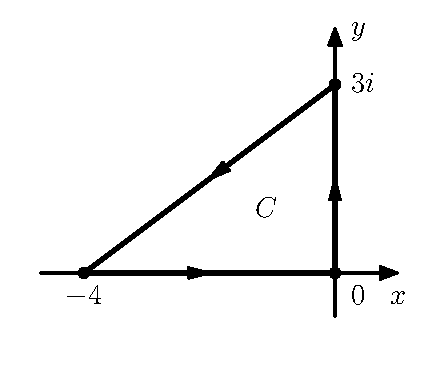
\includegraphics[width=\textwidth]{figuras/exercise_47_03.pdf}
 \end{minipage}\hfill
 \begin{minipage}[c]{0.55\textwidth}
  \caption{
       Contorno empleado en el ejercicio 3.
  }\label{fig:exercise_47_03}
 \end{minipage}
\end{figure}

\emph{Sugerencia:} notar que \(|e^z-\overline{z}|\leq e^x+\sqrt{x^2+y^2}\) cuando \(z=x+iy\).

\paragraph{Solución.} Por un lado se observa que la longitud de \(C\) es (ver la figura \ref{fig:exercise_47_03})
\[
 L=3+4+\sqrt{3^2+4^2}=3+4+5=12.
\]
Además, el módulo del integrando cumple que 
\[
 |e^z-\overline{z}|\leq|e^z|+|\overline{z}|=|e^xe^{iy}|+|x-iy|=e^x+\sqrt{x^2+y^2}\overset{(a)}{\leq}1+4=5,
\]
donde en \((a)\) se tuvo en cuenta que en todos los puntos \(z=x+iy\) del contorno, \(x\leq0\) y por lo tanto, \(e^x\leq1\), y además, que el punto del contorno mas alejado del origen es el vértice en \(-4\), y por lo tanto, todos los puntos del contorno cumplen que \(|z|=\sqrt{x^2+y^2}\leq4\). Por lo tanto, de la ecuación \ref{eq:contour_integral_upper_bound}, se tiene que 
\[
 \left|\int_{C}(e^z-\overline{z})\,dz\right|\leq5\times12=60
\]

\subsubsection{Ejercicio 4}

Sea \(C_R\) el semicírculo superior \(|z|=R\), con \(R>2\), en sentido antihorario. Mostrar que 
\[
 \left|\int_{C_R}\frac{2z^2-1}{z^4+5z^2+4}\,dz\right|\leq\frac{\pi R(2R^2+1)}{(R^2-1)(R^2-4)}.
\]
Luego, dividiendo el numerador y el denominador del lado derecho entre \(R^4\), mostrar que el valor de la integral tiende a cero cuando \(R\) tiende a infinito.

\paragraph{Solución.} Se comienza observando que el largo del contorno es
\[
 L=\frac{2\pi R}{2}=\pi R.
\]
Además, en los puntos del contorno, el numerador del integrando cumple que 
\[
 |2z^2-1|\leq|2z^2|+|1|=2|z|^2+1=2R^2+1,
\]
y notando que el polinomio del denominador tiene las raíces dobles \(-1\) y \(-4\) por lo que se puede expresar como
\[
 z^4+5z^2+4=(z^2+1)(z^2+4),
\]
en \(C_R\) el módulo se puede acotar como
\[
 |z^4+5z^2+4|=|z^2+1||z^2+4|\geq\left||z|^2-1\right|\left||z|^2-4\right|=|R^2-1||R^2-4|=(R^2-1)(R^2-4),
\]
donde en la última igualdad se tuvo en cuenta que \(R>2\). Por lo tanto, en \(C_R\) se cumple que 
\[
 \left|\frac{2z^2-1}{z^4+5z^2+4}\right|=\frac{|2z^2-1|}{|z^4+5z^2+4|}\leq\frac{2R^2+1}{(R^2-1)(R^2-4)},
\]
y combinando los resultados resulta en que
\[
 \left|\int_{C_R}\frac{2z^2-1}{z^4+5z^2+4}\,dz\right|\leq\frac{\pi R(2R^2+1)}{(R^2-1)(R^2-4)}.
\]
Además, 
\[
 \lim_{R\to\infty}\left|\int_{C_R}\frac{2z^2-1}{z^4+5z^2+4}\,dz\right|\leq\lim_{R\to\infty}\frac{\pi R(2R^2+1)}{(R^2-1)(R^2-4)}=\lim_{R\to\infty}\frac{2\pi R^3}{R^4}=\lim_{R\to\infty}\frac{2\pi}{R}=0.
\]

\subsubsection{Ejercicio 5}

Sea \(C_R\) el círculo \(|z|=R\) con \(R>1\) en sentido antihorario. Mostrar que 
\[
 \left|\int_{C_R}\frac{\Log z}{z^2}\,dz\right|<2\pi\left(\frac{\pi+\ln R}{R}\right),
\]
y luego emplear la regla de l'Hôpital para mostrar que el valor de la integral tiende a cero cuando \(R\) tiende a infinito.

\paragraph{Solución.} La longitud del contorno es 
\[
 L=2\pi R.
\]
Además, en el contorno, \(z=Re^{i\Theta}\) con \(-\pi<\Theta\leq\pi\), y por lo tanto,
\[
 |\Log z|=|\ln R+i\Theta|\leq|\ln R|+|\Theta|<\ln R+\pi,
\]
donde la desigualdad estricta se debe a que en la rama principal del logaritmo, \(-\pi<\Theta\leq\pi\) (ver la sección \ref{sec:logarithm_branches}). Además, como
\[
 |z^2|=|z|^2=R^2,
\]
se obtiene que 
\[
 \left|\int_{C_R}\frac{\Log z}{z^2}\,dz\right|<2\pi R\frac{\ln R+\pi}{R^2}=2\pi\left(\frac{\ln R+\pi}{R}\right).
\]
Para calcular el límite cuando \(R\) tiende a infinito, se observa que en el lado derecho de la igualdad, tanto el numerador como el denominador tienden a infinito, por lo que se trata de una indeterminación del tipo \(\infty/\infty\). Aplicando la regla de l'Hôpital resulta en que 
\[
 \lim_{R\to\infty}\left|\int_{C_R}\frac{\Log z}{z^2}\,dz\right|<\lim_{R\to\infty}2\pi\left(\frac{\ln R+\pi}{R}\right)=\lim_{R\to\infty}2\pi\frac{1/R}{1}=0.
\]

\subsubsection{Ejercicio 6}

Sea \(C_\rho\) el círculo \(|z|=\rho\) con \(0<\rho<1\) orientado en sentido antihorario y supóngase que \(f(z)\) es analítica en el círculo \(|z|\leq1\). Mostrar que si \(z^{1/2}\) representa alguna rama particular de dicha potencia de \(z\), existe una constante \(M\) independiente de \(\rho\) tal que 
\[
 \left|\int_{C_\rho}z^{1/2}f(z)\,dz\right|\leq2\pi M\sqrt{\rho}.
\]
De esta forma, mostrar que la integral tiende a cero cuando \(\rho\) tiende a cero.

\emph{Sugerencia:} notar que como \(f(z)\) es analítica, y por lo tanto, continua en el disco \(|z|\leq1\), es acotada allí (ver la sección \ref{sec:continuity_definition})

\paragraph{Solución.} La longitud del contorno es
\[
 L=2\pi\rho.
\]
Para encontrar una cota del integrando en el contorno \(|z|=\rho\), se observa primero que de la definición de la función potencia (ver la ecuación \ref{eq:power_function}),
\[
 z^{-1/2}=\exp\left(-\frac{1}{2}\log z\right)=\exp\left[-\frac{1}{2}(\ln|z|+i\theta)\right]=\frac{1}{\sqrt{|z|}}e^{-i\theta/2},
 \qquad 
 |z|>0,\,\alpha<\theta<\alpha+2\pi,
\]
y por lo tanto, en el contorno \(|z|=\rho\), se cumple que 
\[
 |z^{-1/2}|=\left|\frac{1}{\sqrt{\rho}}e^{-i\theta/2}\right|=\frac{1}{\sqrt{\rho}}.
\]
Por otro lado, como \(f(z)\) es analítica y por lo tanto continua en el disco \(|z|\leq1\), del teorema 4 de la sección \ref{sec:continuity_definition}, existe un número \(M\) tal que 
\[
 |f(z)|\leq M 
\]
para todos los puntos \(z\) en \(|z|\leq1\). Empleando estos resultados, se obtiene que 
\[
 |z^{-1/2}f(z)|=|z^{-1/2}||f(z)|\leq\frac{M}{\sqrt{\rho}},
\]
y finalmente
\[
 \left|\int_{C_\rho}z^{1/2}f(z)\,dz\right|\leq2\pi\rho\frac{M}{\sqrt{\rho}}=2\pi M\sqrt{\rho}.
\]
Además, como \(M\) es independiente de \(\rho\),
\[
 \lim_{\rho\to0}\left|\int_{C_\rho}z^{1/2}f(z)\,dz\right|\leq\lim_{\rho\to0}2\pi M\sqrt{\rho}=0.
\]

\subsubsection{Ejercicio 7}

Aplicar la desigualdad \ref{eq:integrals_wt_tringular_inequality} para mostrar que para todos los valores de \(x\) en el intervalo \(-1\leq x\leq1\), las funciones\footnote{Estas funciones son polinomios en \(x\) y se conocen como \emph{polinomios de Legendre}.}
\[
 P_n(x)=\frac{1}{\pi}\int_0^\pi(x+i\sqrt{1-x^2}\cos\theta)^n\,d\theta,
 \qquad\qquad 
 n=0,\,1,\,2,\,\dots,
\]
cumplen que \(P_n(x)\leq1\).

\paragraph{Solución.} Para encontrar una cota del módulo del integrando, se observa que 
\begin{align*}
 |x+i\sqrt{1-x^2}\cos\theta|&=\sqrt{x^2+\left(\sqrt{1-x^2}\cos\theta\right)^2}\\
   &=\sqrt{x^2+(1-x^2)\cos^2\theta}\\
   &\leq\sqrt{x^2+(1-x^2)}\\
   &=1,
\end{align*}
y por lo tanto,
\[
 |(x+i\sqrt{1-x^2}\cos\theta)^n|=(|x+i\sqrt{1-x^2}\cos\theta|)^n\leq1^n=1.
\]
Considerando este resultado y empleando la ecuación \ref{eq:integrals_wt_tringular_inequality} se tiene que
\begin{align*}
 |P_n(x)|&=\frac{1}{\pi}\left|\int_0^\pi(x+i\sqrt{1-x^2}\cos\theta)^n\,d\theta\right|\\
   &\leq\frac{1}{\pi}\int_0^\pi\left|(x+i\sqrt{1-x^2}\cos\theta)^n\right|\,d\theta\\
   &\leq\frac{1}{\pi}\int_0^\pi1\,d\theta\\
   &=\frac{1}{\pi}\theta\bigg|_0^\pi\\
   &=\frac{1}{\pi}(\pi-0)\\
   &=1.
\end{align*}

\subsubsection{Ejercicio 8}

Sea \(C_N\) la frontera del cuadrado formado por las rectas 
\[
 x=\pm\left(N+\frac{1}{2}\right)\pi
 \qquad\qquad\textrm{y}\qquad\qquad
 y=\pm\left(N+\frac{1}{2}\right)\pi,
\]
donde \(N\) es un entero positivo y la orientación de \(C_N\) es en sentido antihorario.
\begin{enumerate}
 \item[(\textit{a})] Con la ayuda de las desigualdades
 \[
  |\sen z|\geq|\sen x|
  \qquad\qquad\textrm{y}\qquad\qquad
  |\sen z|\geq|\senh y|
 \]
 obtenidas en los ejercicios 8(\textit{a}) y 9(\textit{a}) de la sección \ref{sec:zeros_singularities_trigonometric} mostrar que \(|\sen z|\geq1\) en los lados verticales del cuadrado y \(|\sen z|>\senh(\pi/2)\) en los lados horizontales. De esta forma, mostrar que existe una constante positiva \(A\) independiente de \(N\) tal que \(|\sen z|\geq A\) para todos los puntos \(z\) en el contorno \(C_N\).
 \item[(\textit{b})] Empleando el resultado final de la parte (\textit{a}), mostrar que 
 \[
  \left|\int_{C_N}\frac{dz}{z^2\sen z}\right|\leq\frac{16}{(2N+1)\pi A},
 \]
 y por consiguiente, que el valor de la integral tiende a cero cuando \(N\) tiende a infinito.
\end{enumerate}

\paragraph{Solución.} 
\begin{enumerate}
 \item[(\textit{a})] En los lados verticales del cuadrado \(C_N\), se cumple que 
 \[
  |\sen z|\overset{(a)}{\geq}|\sen x|\overset{(b)}{=}\left|\sen\left[\pm\left(N+\frac{1}{2}\right)\pi\right]\right|=\left|\pm\sen\left[\left(N+\frac{1}{2}\right)\pi\right]\right|=\left|\pm(-1)^N\right|=1,
 \]
 donde en \((a)\), con \(z=x+iy\), se empleó el resultado del ejercicio 8(\textit{a}) de la sección \ref{sec:zeros_singularities_trigonometric} y en \((b)\) se tuvo en cuenta que en los lados verticales de \(C_N\),
 \[
  x=\pm\left(N+\frac{1}{2}\right)\pi.
 \]
 Además, en los lados horizontales,
 \begin{align*}
  |\sen z|&\overset{(a)}{\geq}|\senh y|\\
   &\overset{(b)}{=}\left|\senh\left[\pm\left(N+\frac{1}{2}\right)\pi\right]\right|\\
   &\overset{(c)}{=}\left|\pm\senh\left[\left(N+\frac{1}{2}\right)\pi\right]\right|\\
   &\overset{(d)}{=}\senh\left[\left(N+\frac{1}{2}\right)\pi\right]\\
   &\overset{(e)}{>}\senh\frac{\pi}{2},
 \end{align*}
 donde en \((a)\) se empleó el resultado del ejercicio 9(\textit{a}) de la sección \ref{sec:zeros_singularities_trigonometric}, en \((b)\) se evaluó la expresión en las rectas horizontales, en \((c)\) se consideró que la función \(\senh y\) es impar, en \((d)\) que como \(N\) es un número entero positivo, el argumento es positivo y se cumple que \(\senh y\geq0\) si \(y\geq0\), y en \((e)\) que \(\senh y\) es monótonamente creciente, ya que \(\senh'y=\cosh y\geq1\) para todo \(y\), y como \(N\) es un entero positivo, \(\pi/2<(N+1/2)\pi\). 
 
 Combinando los resultados recién obtenidos, se concluye que en los puntos \(z\) en \(C_N\), se cumple que 
 \[
  |\sen z|\geq\min\left(1,\,\senh\frac{\pi}{2}\right)=A,
 \]
 donde se definió la constante \(A\), que claramente es independiente de \(N\).
 \item[(\textit{b})] Se observa que en los puntos \(z\) en \(C_N\) el denominador del integrando cumple que 
 \[
  |z^2\sen z|=|z|^2|\sen z|\overset{(a)}{\geq}\left[\left(N+\frac{1}{2}\right)\pi\right]^2A=\frac{1}{4}(2N+1)^2\pi^2A,
 \]
 donde en \((a)\) se consideró que los puntos mas cercanos al origen en \(C_N\) son los que cumplen que 
 \[
  z=\pm\left(N+\frac{1}{2}\right)\pi+0i
  \qquad\qquad\textrm{y}\qquad\qquad
  z=0\pm\left(N+\frac{1}{2}\right)\pi i,
 \]
 que cumplen que 
 \[
  |z|=\left(N+\frac{1}{2}\right)\pi,
 \]
 concluyendo que en los puntos \(z\) en \(C_N\),
 \[
  |z|\geq\left(N+\frac{1}{2}\right)\pi,
 \]
 y además se empleó el resultado \(|\sen z|\geq A\) obtenido en la parte (\textit{a}). Esto indica que el módulo del integrando cumple que 
 \[
  \left|\frac{1}{z^2\sen z}\right|\leq\frac{4}{(2N+1)^2\pi^2A}.
 \]

 Por otro lado, la longitud del contorno es 
 \[
  L=4\times2\times\left(N+\frac{1}{2}\right)\pi=4(2N+1)\pi
 \]
 
 Finalmente, combinando los resultados, se obtiene que 
 \[
  \left|\int_{C_N}\frac{dz}{z^2\sen z}\right|\leq4(2N+1)\pi\frac{4}{(2N+1)^2\pi^2A}=\frac{16}{(2N+1)\pi A},
 \]
 y como \(A\) es una constante independiente de \(N\) se cumple que 
 \[
  \lim_{N\to\infty}\left|\int_{C_N}\frac{dz}{z^2\sen z}\right|\leq\lim_{N\to\infty}\frac{16}{(2N+1)\pi A}=0.
 \]
\end{enumerate}

\section{Primitivas}\label{sec:antiderivatives}

Como indican las afirmaciones (\textit{a}) y (\textit{b}) al final de la sección \ref{sec:contour_integrals}, para algunas funciones el valor de la integral entre dos puntos \(z_1\) y \(z_2\) es \emph{independiente del camino}. Adicionalmente, el valor de integrales en caminos cerrados es a veces, pero no siempre, cero.

El siguiente teorema se emplea para determinar cuando la integración es independiente del camino y cuando una integral en un camino cerrado vale cero. El teorema contiene una extensión del teorema fundamental del cálculo que simplifica la evaluación de ciertas integrales. La extensión involucra el concepto de \emph{primitiva} de una función continua \(f(z)\) en un dominio \(D\), o una función \(F(z)\) tal que \(F'(z)=f(z)\) para todo \(z\) en \(D\). Notar que una primitiva es necesariamente una función analítica. Notar además que \emph{una primitiva de una función \(f(z)\) dada es única excepto por una constante aditiva}. Esto es porque la derivada de la diferencia \(F(z)-G(z)\) de dos primitivas de una función es nula, y de acuerdo al teorema de la sección \ref{sec:analytic_functions} una función analítica es constante en un dominio \(D\) cuando su derivada es nula en \(D\).

\paragraph{Teorema.} Sea la función \(f(z)\) continua en un dominio \(D\). Si alguna de las siguientes afirmaciones es cierta, también lo son las otras:
\begin{enumerate}
 \item[(\textit{a})] \(f(z)\) tiene una primitiva \(F(z)\) en \(D\);
 \item[(\textit{b})] las integrales de \(f(z)\) sobre contornos enteramente contenidos en \(D\) que se extienden desde un algún punto fijo \(z_1\) hasta otro fijo \(z_2\) tienen todas el mismo valor, que es 
 \[
  \int_{z_1}^{z_2}f(z)\,dz=F(z)\bigg|_{z_1}^{z_2}=F(z_2)-f(z_1),
 \]
 donde \(F(z)\) es la primitiva de la afirmación (\textit{a});
 \item[(\textit{c})] las integrales de \(f(z)\) sobre contorno cerrados contenidos enteramente en \(D\) tienen todas valor cero.
\end{enumerate}

Notar que el teorema solo indica que las tres afirmaciones son verdaderas o las tres son válidas. La demostración se posterga para mas adelante en esta sección. A continuación se incluyen ejemplos del uso del teorema.

\paragraph{Ejemplo 1.} La función \(f(z)=1/z^2\), que es continua en todo el plano excepto en el origen, tiene primitiva \(F(z)=-1/z\) en el dominio \(|z|>0\). Como consecuencia,
\[
 \int_C\frac{dz}{z^2}=0
\]
cuando \(C\) es el círculo unidad orientado positivamente \(z=e^{i\theta}\) con \(-\pi\leq\theta\leq\pi\).  

\paragraph{Ejemplo 2.} La integral de la función \(f(z)=1/z\) sobre el círculo unidad no puede ser evaluada como en el ejemplo anterior. A pesar de que la derivada de cualquier rama \(F(z)\) de \(\log z\) es \(1/z\) (ver la sección \ref{sec:logarithm_branches} y los ejercicios 6 y 7 de esa sección), \(F(z)\) no está definida en el corte de rama y por lo tanto, no es diferenciable allí. En particular, si se emplea el rayo \(\theta=\alpha\) como corte de rama, \(F'(z)\) no existe en el punto en donde el rayo intersecta al círculo \(C\), como se muestra en la figura \ref{fig:example_48_03_C}. Por lo tanto, \(C\) no está enteramente contenido en un dominio en el cual \(F'(z)=1/z\), por lo que no puede emplearse la primitiva. Sin embargo, a continuación se ilustra como puede emplearse una combinación de dos primitivas para evaluar la integral de \(f(z)=1/z\) sobre \(C\). 
\begin{figure}[!htb]
  \begin{minipage}[c]{0.35\textwidth}
    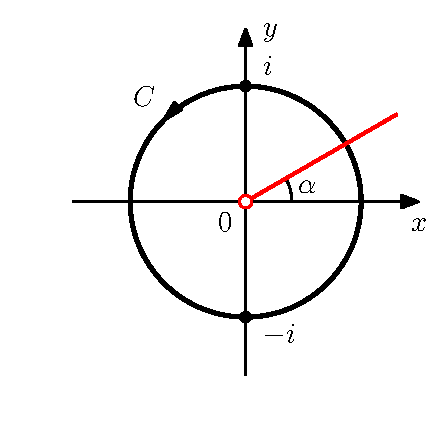
\includegraphics[width=\textwidth]{figuras/example_48_03_C.pdf}
  \end{minipage}\hfill
  \begin{minipage}[c]{0.55\textwidth}
    \caption{
        Corte de rama de la función \(F(z)=\log z\). \(F(z)\) no está definida en el punto de intersección del contorno \(C\) y el corte de rama.
    }\label{fig:example_48_03_C}
  \end{minipage}
\end{figure}

Sea \(C_1\) la mitad derecha
\[
 z=e^{i\theta},
 \qquad\qquad 
 -\frac{\pi}{2}\leq\theta\leq\frac{\pi}{2},
\]
del círculo \(C\) de la figura \ref{fig:example_48_03_C}. La rama principal 
\[
 \Log z=\ln r+i\Theta,
 \qquad\qquad 
 r>0,\,-\pi<\Theta<\pi,
\]
de la función logarítmica sirve de primitiva de la función \(1/z\) en la evaluación de de la integral de \(1/z\) sobre \(C_1\) (ver la figura \ref{fig:example_48_03_C1}):
\[
 \int_{C_1}\frac{dz}{z}=\int_{-i}^i\frac{dz}{z}=\Log z\bigg|_{-i}^i=\Log i-\Log(-i)
 =\left(\ln1+i\frac{\pi}{2}\right)-\left(\ln1-i\frac{\pi}{2}\right)=\pi i.
\]
\begin{figure}[!htb]
  \begin{minipage}[c]{0.35\textwidth}
    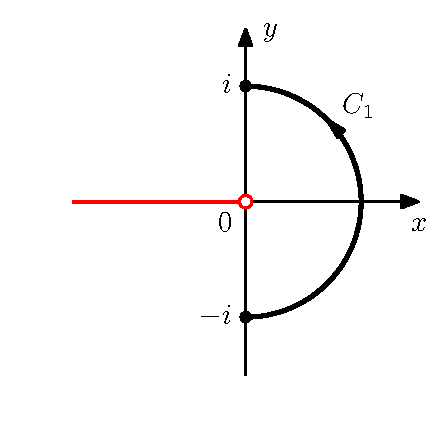
\includegraphics[width=\textwidth]{figuras/example_48_03_C1.pdf}
  \end{minipage}\hfill
  \begin{minipage}[c]{0.55\textwidth}
    \caption{
        Contorno \(C_1\) empleado en el ejemplo 2. El corte de rama de la rama principal \(\Log z\) no intersecta a \(C_1\) por lo que \(\Log z\) es primitiva de \(1/z\) en el contorno de integración.
    }\label{fig:example_48_03_C1}
  \end{minipage}
\end{figure}

Luego, sea \(C_2\) la mitad izquierda 
\[
 z=e^{i\theta},
 \qquad\qquad 
 \frac{\pi}{2}\leq\theta\leq\frac{3\pi}{2},
\]
del círculo mismo círculo \(C\) y se considera la rama
\[
 \log z=\ln r+i\theta,
 \qquad\qquad 
 r>0,\,0<\Theta<2\pi,
\]
de la función logarítmica (ver la figura \ref{fig:example_48_03_C2}). Dicha rama sirve como primitiva de \(1/z\) en la evaluación de la integral sobre \(C_2\):
\[
 \int_{C_2}\frac{dz}{z}=\int_{i}^{-i}\frac{dz}{z}=\log z\bigg|_{i}^{-i}=\log(-i)-\log(i)
 =\left(\ln1+i\frac{3\pi}{2}\right)-\left(\ln1+i\frac{\pi}{2}\right)=\pi i.
\]
\begin{figure}[!htb]
  \begin{minipage}[c]{0.35\textwidth}
    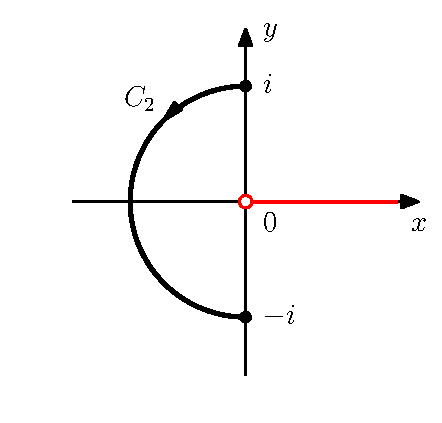
\includegraphics[width=\textwidth]{figuras/example_48_03_C2.pdf}
  \end{minipage}\hfill
  \begin{minipage}[c]{0.55\textwidth}
    \caption{
        Contorno \(C_2\) empleado en el ejemplo 2.
    }\label{fig:example_48_03_C2}
  \end{minipage}
\end{figure}

El valor de la integral de \(1/z\) sobre el círculo \(C=C_1 + C_2\) es por lo tanto
\[
 \int_{C}\frac{dz}{z}=\int_{C_1}\frac{dz}{z}+\int_{C_2}\frac{dz}{z}=\pi i+\pi i=2\pi i.
\]

\paragraph{Ejemplo 3.} Se empleará una primitiva para evaluar la integral
\[
 \int_{C_1}z^{1/2}\,dz,
\]
donde el integrando es la rama 
\begin{equation}\label{eq:example_48_04_funcion_branch}
 f(z)=z^{1/2}=\exp\left(\frac{1}{2}\log z\right)=\sqrt{r}e^{i\theta/2},
 \qquad\qquad
 r>0,\,0<\theta<2\pi,
\end{equation}
de la función raíz cuadrada y \(C_1\) es cualquier contorno desde \(z=-3\) a \(z=3\) que, a excepción de sus extremos, se encuentra enteramente sobre el eje \(x\), como se muestra en la figura \ref{fig:example_48_04}.
\begin{figure}[!htb]
  \begin{minipage}[c]{0.35\textwidth}
    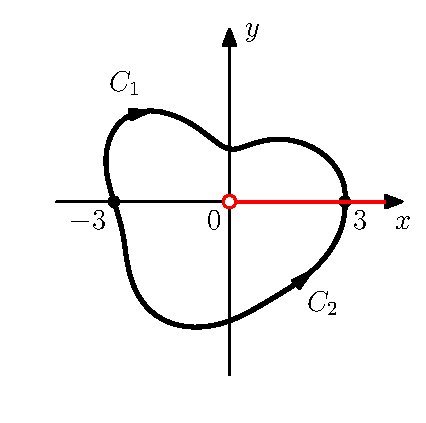
\includegraphics[width=\textwidth]{figuras/example_48_04.pdf}
  \end{minipage}\hfill
  \begin{minipage}[c]{0.55\textwidth}
    \caption{
        Contornos \(C_1\) y \(C_2\) desde \(z=-3\) a \(z=3\) y corte de rama de la función \(f(z)=z^{1/2}\).
    }\label{fig:example_48_04}
  \end{minipage}
\end{figure}
Si bien el integrando es continuo a trozos sobre \(C_1\) y por lo tanto la integral existe, la rama \ref{eq:example_48_04_funcion_branch} de \(z^{1/2}\) no está definida en el rayo \(\theta=0\), y en particular, en el punto \(z=3\). Sin embargo, otra rama
\[
 f_1(z)=\sqrt{r}e^{i\theta/2},
 \qquad\qquad
 r>0,\,-\frac{\pi}{2}<\theta<\frac{3\pi}{2},
\]
está definida y es continua en todos lados sobre \(C_1\). Adicionalmente, los valores de \(f_1(z)\) coinciden con los del integrando \ref{eq:example_48_04_funcion_branch} en todos los puntos de \(C_1\) excepto en \(z=3\) y por lo tanto, el integrando puede reemplazarse por \(f_1(z)\). Como la primitiva de \(f_1(z)\) es la función 
\[
 F_1(z)=\frac{2}{3}z^{3/2}=\frac{2}{3}r\sqrt{r}e^{i3\theta/2},
 \qquad\qquad
 r>0,\,-\frac{\pi}{2}<\theta<\frac{3\pi}{2},
\]
se tiene que 
\begin{equation}\label{eq:example_48_04_integral_C1}
 \int_{C_1}z^{1/2}\,dz=\int_{-3}^3f_1(z)\,dz=F_1(z)\bigg|_{-3}^3\overset{(a)}{=}2\sqrt{3}(e^{i0}-e^{i3\pi/2})
 =2\sqrt{3}[1-(-i)]=2\sqrt{3}(1+i), 
\end{equation}
donde en \((a)\) se tuvo en cuenta que \(3=3e^{i0}\) y \(-3=3e^{i\pi}\), y por lo tanto, \(F_1(3)=2\sqrt{3}e^{i0}\) y \(F_1(-3)=2\sqrt{3}e^{i3\pi/2}\). Comparar este resultado  con el obtenido en el ejemplo de la sección \ref{sec:integrals_examples_with_branch_cuts}.

La integral 
\begin{equation}\label{eq:example_48_04_integral_C2}
 \int_{C_2}z^{1/2}\,dz, 
\end{equation}
de la función \ref{eq:example_48_04_funcion_branch} sobre cualquier contorno \(C_2\) que se extiende desde \(z=-3\) hasta \(z=3\) por debajo del eje real (ver la figura \ref{fig:example_48_04}) puede evaluarse de forma similar. En este caso, se puede reemplazar el integrando por la rama 
\[
 f_2(z)=\sqrt{r}e^{i\theta/2},
 \qquad\qquad
 r>0,\,\frac{\pi}{2}<\theta<\frac{5\pi}{2},
\]
cuyos valores coinciden con el integrando en \(z=-3\) y en todos los puntos de la curva \(C_2\) por debajo del eje real. Teniendo en cuenta estas consideraciones, es posible emplear la primitiva de \(f_2(z)\) para evaluar la integral \ref{eq:example_48_04_integral_C2}, como se hace en el ejercicio 4. 

\subsection*{Prueba del teorema}

Para probar el teorema de esta sección alcanza con mostrar que la afirmación (\textit{a}) implica la afirmación (\textit{b}), que la afirmación (\textit{b}) implica la afirmación (\textit{c}) y que la afirmación (\textit{c}) implica la afirmación (\textit{a}). De esta forma, las tres afirmaciones son verdaderas o las tres son falsas.

\subsubsection*{(\textit{a}) implica (\textit{b})}

Se comienza con la hipótesis de la afirmación (\textit{a}) es verdadera, o que \(f(z)\) tiene una primitiva \(F(z)\) en el dominio \(D\). Para mostrar que se cumple la afirmación (\textit{b}) hay que probar que la integración es independiente del camino en \(D\) y que el teorema fundamental del cálculo puede extenderse empleando \(F(z)\). 

Si un contorno \(C\) desde \(z_1\) hasta \(z_2\) es un arco suave contenido en \(D\) con representación paramétrica \(z(t)\) con \(a\leq t\leq b\), del ejercicio 5 de la sección \ref{sec:contours} se tiene que 
\[
 \frac{d}{dt}F[z(t)]=F'[z(t)]z'(t)=f[z(t)]z'(t),
 \qquad\qquad
 a\leq t\leq b.
\]
Pero como se mostró en la sección \ref{sec:definite_integrals_wt}, el teorema fundamental del cálculo puede extenderse a funciones complejas de variable real, y por lo tanto
\[
 \int_Cf(z)\,dz=\int_a^bf[z(t)]z'(t)\,dt=F[z(t)]\bigg|_a^b=F[z(b)]-F[z(a)]=F(z_2)-F(z_1).
\]
Se obtuvo que el valor de la integral de contorno es \(F(z_2)-F(z_1)\), independiente del contorno \(C\) mientras \(C\) se extienda desde \(z_1\) hasta \(z_2\) enteramente en el dominio \(D\). Se concluye que cuando \(C\) es una arco suave,
\[
 \int_Cf(z)\,dz=F(z_2)-F(z_1)=F[z(b)]-F[z(a)],
\]
que es el teorema fundamental del cálculo para una función compleja. Esta expresión también es válida cuando \(C\) es cualquier arco, no necesariamente suave, contenido enteramente en \(D\). Esto concluye la prueba de que la afirmación (\textit{b}) surge de la afirmación (\textit{a}). 

\subsubsection*{(\textit{b}) implica (\textit{c})}

Para verificar que la afirmación (\textit{b}) implica la afirmación (\textit{c}) se asume ahora que la integración de \(f(z)\) es independiente del camino en \(D\) y se mostrará que los valores de las integrales de \(f(z)\) en caminos cerrados en \(D\) es siempre cero.

Sean \(z_1\) y \(z_2\) dos puntos pertenecientes a algún contorno cerrado \(C\) dentro del dominio \(D\), y se forman los caminos \(C_1\) y \(C_2\) que van desde el punto inicial \(z_1\) hasta el punto final \(z_2\) tal que \(C=C_1-C_2\), como se muestra en la figura \ref{fig:antiderivatives_theorem}.
\begin{figure}[!htb]
  \begin{minipage}[c]{0.45\textwidth}
    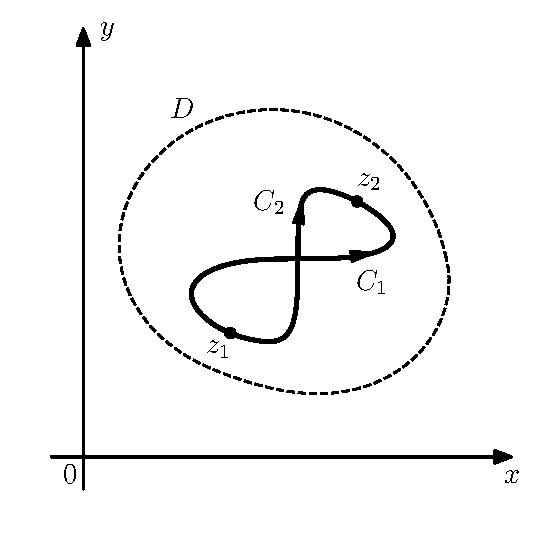
\includegraphics[width=\textwidth]{figuras/antiderivatives_theorem.pdf}
  \end{minipage}\hfill
  \begin{minipage}[c]{0.45\textwidth}
    \caption{
        Contorno cerrado \(C\) en \(D\). Se construyen los contornos \(C_1\) y \(C_2\) desde el punto \(z_1\) hasta el punto \(z_2\) tal que \(C=C_1-C_2\).
    }\label{fig:antiderivatives_theorem}
  \end{minipage}
\end{figure}
Asumiendo que la integración es independiente del camino en \(D\), se cumple que 
\begin{equation}\label{eq:antiderivatives_theorem_two_paths}
 \int_{C_1}f(z)\,dz=\int_{C_2}f(z)\,dz, 
\end{equation}
es decir,
\begin{equation}\label{eq:antiderivatives_theorem_closed_paths}
 \int_{C_1}f(z)\,dz+\int_{-C_2}f(z)\,dz=0. 
\end{equation}
Se concluye que la integral de \(f(z)\) sobre el contorno cerrado \(C=C_1-C_2\) tiene valor cero.

\subsubsection*{(\textit{c}) implica (\textit{a})}

Falta demostrar que si la integral de una función \(f(z)\) sobre contornos cerrados en \(D\) tiene siempre valor cero, entonces \(f(z)\) tiene primitiva en \(D\).

Asumiendo que los valores de las integrales en caminos cerrados es siempre cero, se comenzará mostrando que la integración es independiente del camino en \(D\), es decir, que (\textit{c}) implica (\textit{b}). Sean \(C_1\) y \(C_2\) dos contornos qualiera en \(D\) desde el punto \(z_1\) hasta el punto \(z_2\) y se observa que como las integrales en caminos cerrados en \(D\) tienen valor cero, se cumple la ecuación \ref{eq:antiderivatives_theorem_closed_paths} (ver la figura \ref{fig:antiderivatives_theorem}), y como consecuencia se cumple la ecuación \ref{eq:antiderivatives_theorem_two_paths}. Se concluye que la integración es independiente del camino en \(D\), por lo que se puede definir la función
\[
 F(z)=\int_{z_0}^zf(s)\,ds
\]
en \(D\). La prueba se completa si se muestra que \(F'(z)=f(z)\) en todos lados en \(D\). Para hacerlo, sea \(z+\Delta z\) un punto distinto de \(z\) en algún entorno de \(z\) suficientemente pequeño de forma de estar contenido en \(D\). Entonces,
\begin{equation}\label{eq:antiderivatives_theorem_incremental}
  F(z+\Delta z)-F(z)=\int_{z_0}^{z+\Delta z}f(s)\,ds-\int_{z_0}^zf(s)\,ds=\int_{z}^{z+\Delta z}f(s)\,ds,
\end{equation}
donde el camino de integración puede elegirse como la recta que une \(z\) y \(z+\Delta z\) de forma de asegurar que está contenido en \(D\). Como
\[
 \int_{z}^{z+\Delta z}\,ds=\Delta z,
\]
como se mostró en el ejercicio 5 de la sección \ref{sec:integrals_examples_with_branch_cuts}, se cumple que 
\[
 \frac{1}{\Delta z}\int_{z}^{z+\Delta z}\,ds=1
\]
y al multiplicar ambos lados de la igualdad por \(f(z)\) resulta en que 
\[
 f(z)=\frac{1}{\Delta z}\int_{z}^{z+\Delta z}f(z)\,ds.
\]
Dividiendo ambos lados de la igualdad \ref{eq:antiderivatives_theorem_incremental} entre \(\Delta z\) y luego restando \(f(z)\) en ambos de la igualdad empleando el último resultado, se obtiene que 
\begin{align*}
 \frac{F(z+\Delta z)-F(z)}{\Delta z}-f(z)&=\frac{1}{\Delta z}\int_{z}^{z+\Delta z}f(s)\,ds-\frac{1}{\Delta z}\int_{z}^{z+\Delta z}f(z)\,ds\\
 &=\frac{1}{\Delta z}\int_{z}^{z+\Delta z}[f(s)-f(z)]\,ds. 
\end{align*}
Pero \(f\) es continua en el punto \(z\). Por lo tanto, para cada número positivo \(\epsilon\), existe un número positivo \(\delta\) tal que (ver la ecuación \ref{eq:continuity_definition})
\[
 |f(s)-f(z)|<\epsilon\qquad\textrm{si}\qquad|s-z|<\delta. 
\]
Por lo tanto, si el punto \(z+\Delta z\) está suficientemente cerca de \(z\) de forma tal que \(|\Delta z|<\delta\) se cumple que
\begin{align*}
 \left|\frac{F(z+\Delta z)-F(z)}{\Delta z}-f(z)\right|&=\frac{1}{|\Delta z|}\left|\int_{z}^{z+\Delta z}[f(s)-f(z)]\,ds\right|\\ 
 &\overset{(a)}{<}\frac{1}{|\Delta z|}\epsilon|\Delta z|\\
 &=\epsilon,
\end{align*}
donde en \((a)\) se empleó el resultado de la ecuación \ref{eq:contour_integral_upper_bound} y se consideró que el camino es un segmento y por lo tanto su longitud es \(|\Delta z|\). Se concluye que como 
\[
 \left|\frac{F(z+\Delta z)-F(z)}{\Delta z}-f(z)\right|<\epsilon
 \qquad\textrm{si}\qquad|\Delta z|<\delta,
\]
de la definición de límite de la ecuación \ref{eq:limit_definition} se cumple que 
\[
 \lim_{\Delta z\to0}\frac{F(z+\Delta z)-F(z)}{\Delta z}=f(z),
\]
y de la definición de derivada de la ecuación \ref{eq:derivative_definition_delta_z},
\[
 F'(z)=f(z),
\]
que es lo que se quería demostrar.

\subsection*{Ejercicios}

\subsubsection*{Ejercicio 1}

Emplear una primitiva para mostrar que para cada contorno \(C\) que se extiende desde un punto \(z_1\) hasta un punto \(z_2\),
\[
 \int_Cz^n\,dz=\frac{1}{n+1}\left(z_2^{n+1}-z_1^{n+1}\right),
 \qquad\qquad
 n=0,\,1,\,2,\,\dots.
\]

\paragraph{Solución.} El integrando \(z^n\) tiene primitiva \(z^{n+1}/(n+1)\) en todo el plano complejo. Por lo tanto, del teorema de la sección \ref{sec:antiderivatives}, la integral en cualquier contorno depende solo de los puntos inicial y final y no del camino. De esta forma,
\[
 \int_Cz^n\,dz=\int_{z_1}^{z_2}z^n\,dz=\frac{z^{n+1}}{n+1}\bigg|_{z_1}^{z_2}=\frac{1}{n+1}\left(z_2^{n+1}-z_1^{n+1}\right).
\]

\subsubsection*{Ejercicio 2}

Evaluar las siguientes integrales encontrando una primitiva, donde el contorno es cualquier camino entre los límites de integración indicados:
\[
 (\textit{a})\;\int_0^{i+1}z^2\,dz;\qquad\qquad(\textit{b})\;\int_0^{\pi+2i}\cos\left(\frac{z}{2}\right)\,dz;
 \qquad\qquad(\textit{c})\;\int_1^3(z-2)^3\,dz.
\]

\paragraph{Solución.} Las  funciones de los integrandos tienen primitiva en todo el plano complejo, y por lo tanto, las integrales solo dependen de los límites de integración.
\begin{enumerate}
 \item[(\textit{a})] 
 \[
  \int_0^{i+1}z^2\,dz=\frac{z^3}{3}\bigg|_0^{i+1}=\frac{1}{3}\left[(1+i)^3-0^3\right]=\frac{1}{3}\left(\sqrt{2}e^{i\pi/4}\right)^3
  =\frac{2}{3}\left(\sqrt{2}e^{i3\pi/4}\right)=\frac{2}{3}(-1+i).
 \]
 \item[(\textit{b})] 
 \begin{align*}
  \int_0^{\pi+2i}\cos\left(\frac{z}{2}\right)\,dz&=2\sen\left(\frac{z}{2}\right)\bigg|_0^{\pi+2i}\\
   &=2\left[\sen\left(\frac{\pi}{2}+i\right)-\sen0\right]\\
   &=2\frac{e^{i(\pi/2+i)}-e^{-i(\pi/2+i)}}{2i}\\
   &=-i\left(e^{i\pi/2}e^{-1}-e^{-i\pi/2}e\right)\\
   &=-i\left[\frac{i}{e}-(-i)e\right]\\
   &=\frac{1}{e}+e.
 \end{align*}
 \item[(\textit{c})]
 \[
  \int_1^3(z-2)^3\,dz=\frac{(z-2)^4}{4}\bigg|_1^3=\frac{1}{4}\left[1^4-(-1)^4\right]=\frac{1}{4}(1-1)=0.
 \]
\end{enumerate}

\subsubsection*{Ejercicio 3}

Emplear el teorema de la sección \ref{sec:antiderivatives} para mostrar que 
\[
 \int_{C_0}(z-z_0)^{n-1}\,dz=0,
 \qquad\qquad
 n=\pm1,\,\pm2,\,\dots,
\]
cuando \(C_0\) es cualquier contorno cerrado que no pasa con el punto \(z=z_0\). Comparar con el ejercicio 13 de la sección \ref{sec:integrals_examples_with_branch_cuts}.

\paragraph{Solución.} La función \((z-z_0)^{n-1}\) con \(n=\pm1,\,\pm2,\,\dots\) tiene primitiva en cualquier dominio del plano complejo que no incluya al punto \(z=z_0\). Por lo tanto, del teorema de la sección \ref{sec:antiderivatives},
\[
 \int_{C_0}(z-z_0)^{n-1}\,dz=0
\]
en cualquier contorno \(C_0\) cerrado que no pase por el punto \(z=z_0\).

\subsubsection*{Ejercicio 4}

Encontrar una primitiva \(F_2(z)\) de la rama \(f_2(z)\) de \(z^{1/2}\) del ejemplo 3 de la sección \ref{sec:antiderivatives} para mostrar que la integral \ref{eq:example_48_04_integral_C2} vale \(2\sqrt{3}(-1+i)\). Notar que el valor de la integral de la función \ref{eq:example_48_04_funcion_branch} alrededor del contorno \(C_2-C_1\) en ese ejemplo es, por lo tanto, \(-4\sqrt{3}\).

\paragraph{Solución.} Recurriendo al ejemplo 3 de la sección \ref{sec:antiderivatives}, la rama 
\[
 f_2(z)=\sqrt{r}e^{i\theta/2},
 \qquad\qquad
 r>0,\,\frac{\pi}{2}<\theta<\frac{5\pi}{2},
\]
de la función \(z^{1/2}\) coincide con la rama del integrando \ref{eq:example_48_04_funcion_branch} en el punto \(z=-3\) y el resto de los puntos de la curva \(C_2\) en la mitad inferior del plano complejo, y tiene primitiva \(F_2(z)\) en todos los puntos en \(C_2\), la cual está dada por 
\[
 F_2(z)=\frac{2}{3}z^{3/2}=\frac{2}{3}(re^i\theta)^{3/2}=\frac{2}{3}r\sqrt{r}e^{i3\theta/2},
 \qquad\qquad
 r>0,\,\frac{\pi}{2}<\theta<\frac{5\pi}{2}.
\]
Por lo tanto, 
\[
 \int_{C_2}z^{1/2}\,dz=\int_{-3}^3f_2(z)\,dz=F_2(z)\bigg|_{-3}^3\overset{(a)}{=}\frac{2}{3}3\sqrt{3}\left(e^{i3\pi}-e^{i3\pi/2}\right)=2\sqrt{3}\left[-1-(-i)\right]=2\sqrt{3}(-1+i),
\]
donde en \((a)\) se tuvo en cuenta que en la rama elegida, \(3=3e^{i2\pi}\) y \(-3=3e^{i\pi}\).

Finalmente, en el contorno cerrado \(C_2-C_1\) orientado positivamente, se cumple que 
\[
 \int_{C_2-C_1}z^{1/2}\,dz=\int_{C_2}z^{1/2}\,dz-\int_{C_1}z^{1/2}\,dz=2\sqrt{3}(-1+i)-2\sqrt{3}(1+i)=-4\sqrt{3},
\]
donde se empleó el resultado de la ecuación \ref{eq:example_48_04_integral_C1} en el ejemplo 3.

\subsubsection*{Ejercicio 5}

Mostrar que 
\[
 \int_{-1}^1z^i\,dz=\frac{1+e^{-\pi}}{2}(1-i)
\]
donde el integrando es la rama principal 
\[
 z^i=\exp(i\Log z),
 \qquad\qquad
 |z|>0,\,-\pi<\Arg z<\pi,
\]
de \(z^i\) y donde el camino de integración es cualquier contorno desde \(z=-1\) hasta \(z=1\) que, excepto por sus puntos extremos, yace sobre el eje real. Comparar con el ejercicio 6 de la sección \ref{sec:integrals_examples_with_branch_cuts}.

\emph{Sugerencia:} emplear la primitiva de la rama 
\[
 z^i=\exp(i\log z),
 \qquad\qquad
 |z|>0,\,-\frac{\pi}{2}<\arg z<\frac{3\pi}{2},
\]
de la misma función potencia.

\paragraph{Solución.} La rama principal de la función \(z^i\)
\[
 z^i=\exp(i\Log z),
 \qquad\qquad
 |z|>0,\,-\pi<\Arg z<\pi,
\]
no está definida en el punto \(z=-1\) del contorno de integración, y por lo tanto, no tiene primitiva allí. Pero la rama
\[
 f_1(z)=z^i=\exp(i\log z),
 \qquad\qquad
 |z|>0,\,-\frac{\pi}{2}<\arg z<\frac{3\pi}{2},
\]
tiene primitiva \(F_1(z)\) en todos los puntos del contorno de integración y sus valores coinciden con los valores de la rama principal en \(z=1\) y en todos los puntos del contorno en el semiplano superior, donde 
\[
 F_1(z)=\frac{z^{i+1}}{i+1},
 \qquad\qquad
 |z|>0,\,-\frac{\pi}{2}<\arg z<\frac{3\pi}{2}.
\]
Por lo tanto,
\begin{align*}
 \int_{-1}^1z^i\,dz&=\int_{-1}^1f_1(z)\,dz\\
  &=F_1(z)\bigg|_{-1}^1\\
  &=\frac{z^{i+1}}{i+1}\bigg|_{-1}^1\\
  &=\frac{1}{i+1}\left[1^{i+1}-(-1)^{i+1}\right]\\
  &\overset{(a)}{=}\frac{1}{i+1}\left\{\exp\left[(i+1)(\ln1+i0)\right]-\exp\left[(i+1)(\ln1+i\pi)\right]\right\}\\
  &=\frac{1}{i+1}\left\{\exp0-\exp\left[(i+1)i\pi\right]\right\}\\
  &=\frac{1}{i+1}\left(e^0-e^{-\pi}e^{i\pi}\right)\\
  &=\frac{1-i}{2}(1+e^{-\pi}),
\end{align*}
donde en \((a)\) se consideró que en la rama empleada, \(1=1e^{i0}\) y \(-1=1e^{i\pi}\). 

Observar que en el ejercicio 6 de la sección \ref{sec:integrals_examples_with_branch_cuts} se calculó la integral de la misma función sobre el semicírculo superior orientado positivamente, y como la integral no depende del camino de integración pero en este caso el camino de integración tiene orientación negativa, se obtuvo el resultado opuesto.

\section{Teorema de Cauchy-Goursat}\label{sec:cauchy_goursat_theorem}

En la sección \ref{sec:antiderivatives} se vio que cuando una función continua \(f\) tiene primitiva en un dominio \(D\), la integral de \(f(z)\) sobre un contorno cerrado \(C\) contenido completamente en \(D\) tiene valor cero. En esta sección se presenta un teorema que establece otras condiciones sobre la función \(f\) que aseguran que la integral sobre un \emph{contorno cerrado simple} (ver la sección \ref{sec:contours}) vale cero. El teorema es central en la teoría de funciones de variable compleja, y algunas variantes que involucran ciertos tipos de dominio se verán en las secciones \ref{sec:simply_connected_domains} y \ref{sec:multiply_connected_domains}. 

Sea \(C\) un contorno cerrado simple \(z=z(t)\) donde \(a\leq t\leq b\), con orientación positiva, y asúmase que \(f\) es analítica en cada punto interior y sobre \(C\). De acuerdo a la ecuación \ref{eq:contour_integral_definition}
\[
 \int_C f(z)\,dz=\int_a^b f[z(t)]z'(t)\,dz,
\]
y si 
\[
 f(z)=u(x,\,y)+iv(x,\,y)
 \qquad\qquad\textrm{y}\qquad\qquad
 z(t)=x(t)+iy(t),
\]
el integrando es la función
\begin{align*}
 f[z(t)]z'(t)&=\left\{u[x(t),\,y(t)]+iv[x(t),\,y(t)]\right\}\left[x'(t)+iy'(t)\right]\\
  &=\left\{u[x(t),\,y(t)]x'(t)-v[x(t),\,y(t)]y'(t)\right\}+i\left\{v[x(t),\,y(t)]x'(t)+u[x(t),\,y(t)]y'(t)\right\}
\end{align*}
de variable real \(t\). Por lo tanto,
\[
 \int_C f(z)\,dz=\int_a^b(ux'-vy')\,dt+i\int_a^b(vx'+uy')\,dt.
\]
En términos de integrales de contorno de funciones reales de dos variables reales, el resultado se puede expresar como
\begin{equation}\label{eq:cauchy_goursat_previous_line_integral}
 \int_C f(z)\,dz=\int_C u\,dx-v\,dy+i\int_C v\,dx+u\,dy. 
\end{equation}
Las integrales del lado derecho en esta igualdad se denominan integrales de línea sobre el contorno \(C\) respecto a \(x\) o a \(y\) (ver la sección 16.2 de \cite{stewart2016essential}). Observar que la ecuación \ref{eq:cauchy_goursat_previous_line_integral} también se puede obtener formalmente reemplazando \(f(z)\) y \(dz\) en el lado izquierdo por \(u+iv\) y \(dx+idy\) respectivamente y expandiendo su producto. La ecuación \ref{eq:cauchy_goursat_previous_line_integral} es válida cuando \(C\) es cualquier contorno y no necesariamente uno cerrado simple, y cuando \(f[z(t)]\) es solamente continua a trozos en él.

Para continuar, se considerará un resultado de cálculo que permite expresar las integrales de línea del lado derecho de la ecuación \ref{eq:cauchy_goursat_previous_line_integral} como integrales dobles.

\medskip
\noindent
\fbox{%
\begin{minipage}{\textwidth}
\paragraph{Teorema de Green.} Sea \(C\) un contorno cerrado simple orientado positivamente y sea \(R\) la región que consiste en todos los puntos interiores y sobre \(C\). Si las funciones reales \(P(x,\,y)\) y \(Q(x,\,y)\) tienen derivadas parciales de primer orden continuas en una región abierta que contiene a \(R\), se cumple que 
\[
 \int_C P\,dx+Q\,dy=\iint_R(Q_x-P_y)\,dA.
\]


\medskip
El enunciado y la demostración para un caso particular del teorema puede encontrarse en la sección 16.4 de \cite{stewart2016essential} o en la sección 15.4 de \cite{larson2009calculus}. 
\end{minipage}} 

\medskip 
\noindent
El teorema de Green permite escribir la ecuación \ref{eq:cauchy_goursat_previous_line_integral} como
\begin{equation}\label{eq:cauchy_goursat_theorem_contour_integral_with_green_theorem}
 \int_C f(z)\,dz=\iint_R(-v_x-u_y)\,dA+i\iint_R(u_x-v_y)\,dA,  
\end{equation}
y considerando las ecuaciones de Cauchy-Riemann
\[
 u_x=v_y
 \qquad\qquad\textrm{y}\qquad\qquad
 u_y=-v_x,
\]
se observa que los integrandos de las integrales dobles son cero en \(R\). Se concluye que cuando \(f\) es analítica en \(R\) y \(f'\) es continua allí, 
\[
 \int_C f(z)\,dz=0. 
\]
Notar que una vez que se estableció que la integral es cero, la orientación de \(C\) es irrelevante. Este resultado fue obtenido por Cauchy en la primera parte del siglo diecinueve.\footnote{El resultado fue publicado por Augustin-Louis Cauchy en el libro ``Mémoire sur les intégrales définies, prises entre des limites imaginaires,'' submitted to the Académie des Sciences on February 28: Paris, De Bure frères. 1825.}

Goursat fue el primero en probar que la condición de continuidad sobre \(f'\), que proviene del uso del teorema de Green en la demostración de Cauchy, puede ser omitida. Esta remoción es importante y permite mostrar, por ejemplo, que la derivada \(f'\) de una función analítica \(f\) es analítica sin tener que asumir la continuidad de \(f'\), hecho que surge como consecuencia. A continuación se establece la forma revisada del resultado de Cauchy, que se conoce como el \emph{teorema de Cauchy-Goursat} o \emph{teorema integral de Cauchy}.

\paragraph{Teorema.} Si una función \(f\) es analítica en todos los puntos interiores y sobre un contorno cerrado simple \(C\), se cumple que 
\begin{equation}\label{eq:cauchy_goursat_theorem}
 \int_C f(z)\,dz=0.  
\end{equation}
La prueba del teorema se incluye en la siguiente sección.

\section{Prueba del teorema de Cauchy-Goursat}\label{sec:cauchy_goursat_theorem_proof}

Como la prueba del teorema es mas bien larga, se presentará dividida en tres partes.

\subsection*{Lema preliminar}

En esta sección se presenta un lema que será empleado en la prueba del teorema. En el lema, se forman subconjuntos de la región \(R\), que consiste en los puntos del contorno cerrado simple \(C\) orientado positivamente junto a los puntos interiores a \(C\). Para construir los subconjuntos, se dibujan líneas equiespaciadas paralelas a los ejes \(x\) y \(y\) tal que la distancia entre líneas adyacentes verticales es la misma que entre líneas adyacentes horizontales. Así, se obtiene un conjunto finito de subregiones cerradas cuadradas, donde cada punto de \(R\) se encuentra en al menos una subregión y cada subregión contiene puntos de \(R\). Las subregiones cuadradas serán referidas simplemente como \emph{cuadrados}, teniendo en cuenta que un cuadrado consiste en la frontera y los puntos  interiores a el. Si un cuadrado contiene puntos que no están en \(R\), se eliminan esos puntos y lo que queda se llamará \emph{cuadrado parcial}. De esta forma, se cubre la región \(R\) con un número finito de cuadrados y cuadrados parciales, como se muestra en la figura \ref{fig:cauchy_goursat_lemma_mesh}. Para la prueba del siguiente lema se comienza con esta cobertura de la región \(R\).
\begin{figure}[!htb]
  \begin{minipage}[c]{0.5\textwidth}
    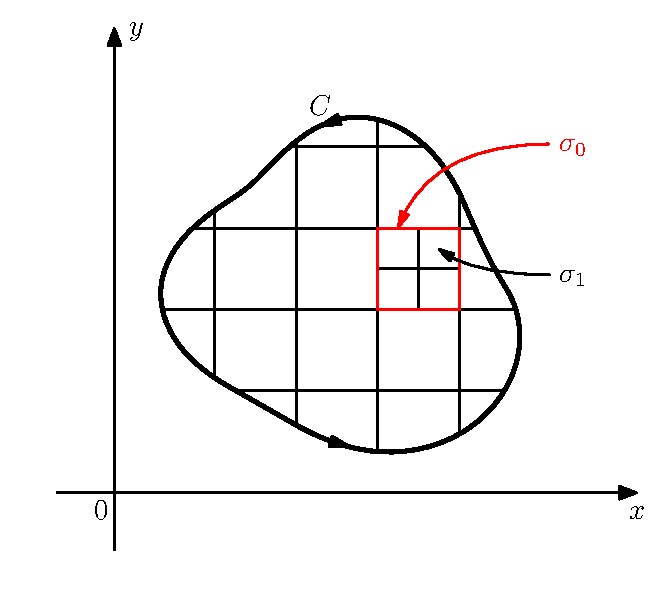
\includegraphics[width=\textwidth]{figuras/cauchy_goursat_lemma_mesh.pdf}
  \end{minipage}\hfill
  \begin{minipage}[c]{0.4\textwidth}
    \caption{
       División de la región \(R\) en cuadrados y cuadrados parciales.
    }\label{fig:cauchy_goursat_lemma_mesh}
  \end{minipage}
\end{figure}

\paragraph{Lema.} Sea \(f\) una función analítica en una región cerrada \(R\) que consiste en los puntos interiores a un contorno \(C\) cerrado simple junto con los puntos en \(C\). Para cada número positivo \(\epsilon\), la región \(R\) puede ser cubierta con un número finito de cuadrados y cuadrados parciales, indexados como \(j=1,\,2,\,\dots,\,n\), de forma tal que en cada uno existe un punto fijo \(z_j\) para el cual la desigualdad
\begin{equation}\label{eq:cauchy_goursat_lemma_inequality}
 \left|\frac{f(z)-f(z_j)}{z-z_j}-f'(z_j)\right|<\epsilon 
\end{equation}
se cumple para todos los puntos distintos a \(z_j\) en el cuadrado o cuadrado parcial.

Para comenzar la prueba, se considera la posibilidad de que en la cobertura construida, haya algún cuadrado o cuadrado parcial en el cual no exista un punto \(z_j\) tal que la desigualdad \ref{eq:cauchy_goursat_lemma_inequality} se cumpla para todos los otros puntos \(z\) en el. Si dicha subregión es un cuadrado, se construyen cuatro cuadrados mas pequeños dibujando segmentos de recta que unen los puntos medios de los lados opuestos, como se muestra en la figura \ref{fig:cauchy_goursat_lemma_mesh}. Si la subregión es un cuadrado parcial, se trata al cuadrado entero de la misma forma y luego se descartan los puntos exteriores a \(R\). Si en alguna de estas subregiones mas pequeñas no existe un punto \(z_j\) tal que la desigualdad \ref{eq:cauchy_goursat_lemma_inequality} se cumpla para todos los otros puntos \(z\) en ella, se construyen cuadrados y cuadrados parciales mas pequeños, y así sucesivamente. Al hacer esto para cada subregión original que lo requiera, se encuentra que \emph{luego de un número finito de pasos}, la región \(R\) es cubierta con un número finito de cuadrados y cuadrados parciales de forma tal que el lema se cumple.

Para verificar esto, supóngase que no existen los puntos \(z_j\) requeridos luego de dividir alguna de las subregiones originales un número finito de veces y así llegar a una contradicción. Se denota a esa subregión como \(\sigma_0\) si es un cuadrado; si es un cuadrado parcial \(\sigma_0\) denota al cuadrado entero del cual es parte. Luego de subdividir \(\sigma_0\), al menos uno de los cuatro cuadrados mas pequeños, denotado como \(\sigma_1\), debe contener puntos de \(R\) pero no un punto \(z_j\) apropiado. Luego se subdivide \(\sigma_1\) y así sucesivamente. Luego de que se subdividió el cuadrado \(\sigma_{k-1}\) (\(k=1,\,2,\,\dots\)), puede elegirse mas de uno de los cuadrados mas pequeños construidos a partir de el. Para realizar una elección específica se toma \(\sigma_k\) como el cuadrado que está mas abajo y luego mas a la izquierda. [¿Por qué se necesita especificar un orden? En otras demostraciones, no se incluye este comentario].

Por la forma en que la secuencia anidada infinita 
\begin{equation}\label{eq:cauchy_goursat_lemma_sequence}
 \sigma_0,\,\sigma_1,\,\dots,\,\sigma_{k-1},\,\sigma_k,\,\dots
\end{equation}
de cuadrados fue construida, puede mostrarse que hay un punto \(z_0\) común a cada \(\sigma_k\), como se hace en el ejercicio 9 de la sección \ref{sec:multiply_connected_domains}, y cada uno de los cuadrados tiene puntos de \(R\) además de \(z_0\). Considerando que los cuadrados en la secuencia son decrecientes, notar que cualquier entorno \(\delta\) \(|z-z_0|<\delta\) de \(z_0\) contiene los cuadrados cuyas diagonales tienen longitud menor a \(\delta\). Por lo tanto, cada entorno \(\delta\) \(|z-z_0|<\delta\) contiene puntos de \(R\) además de \(z_0\), y esto significa que \(z_0\) es un punto de acumulación de \(R\). Como la región \(R\) es un conjunto cerrado, \(z_0\) es un punto de \(R\).

Continuando, la función \(f\) es analítica en \(R\), y en particular, en el punto \(z_0\). En consecuencia, \(f'(z_0)\) existe. De acuerdo a la definición de derivada (ver la sección \ref{sec:derivatives}), para cada número positivo \(\epsilon\), existe un entorno \(\delta\) \(|z-z_0|<\delta\) tal que la desigualdad
\[
 \left|\frac{f(z)-f(z_0)}{z-z_0}-f'(z_0)\right|<\epsilon
\]
se cumple para todos los puntos distintos de \(z_0\) en dicho entorno. Pero el entorno \(|z-z_0|<\delta\) contiene un cuadrado \(\sigma_K\) cuando el entero \(K\) es suficientemente grande de forma que la diagonal de dicho cuadrado sea menor que \(\delta\), como se muestra en la figura \ref{fig:cauchy_goursat_lemma_z0}. Por lo tanto, el punto \(z_0\) actúa como punto \(z_j\) en la desigualdad \ref{eq:cauchy_goursat_lemma_inequality} para la subregión de consiste en el cuadrado o cuadrado parcial \(\sigma_K\). De esta forma, considerando como la secuencia \ref{eq:cauchy_goursat_lemma_sequence} fue construida, no es necesario subdividir \(\sigma_K\). Esto conduce a una contradicción y completa la prueba del lema.
\begin{figure}[!htb]
  \begin{minipage}[c]{0.45\textwidth}
    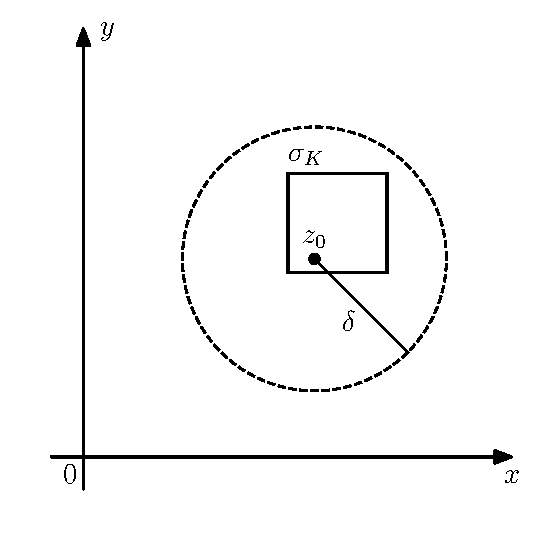
\includegraphics[width=\textwidth]{figuras/cauchy_goursat_lemma_z0.pdf}
  \end{minipage}\hfill
  \begin{minipage}[c]{0.45\textwidth}
    \caption{
        El entorno \(\delta\) de \(z_0\) contiene el cuadrado \(\sigma_K\) cuando \(K\) es lo suficientemente grande.
    }\label{fig:cauchy_goursat_lemma_z0}
  \end{minipage}
\end{figure}

\subsection*{Una cota superior para el módulo de la integral}

Continuando con una función \(f\) que es analítica en una región \(R\) que consiste en un contorno \(C\) cerrado simple orientado positivamente y los puntos interiores a el, se probará el teorema de Cauchy-Goursat, es decir, que 
\[
 \int_Cf(z)\,dz=0.
\]

Dado un número positivo arbitrario \(\epsilon\), se considera la cobertura de \(R\) establecida en el lema. Luego, en el cuadrado o cuadrado parcial \(j\)-ésimo se define la función \(\delta_j(z)\) como
\[
 \delta_j(z)=
 \left\{
 \begin{array}{ll}
  \dfrac{f(z)-f(z_j)}{z-z_j}-f'(z_j), & z\neq z_j\\
  0, & z=z_j,
 \end{array}
 \right.
\]
donde \(z_j\) es el punto fijo de la desigualdad \ref{eq:cauchy_goursat_lemma_inequality}. De acuerdo a la desigualdad \ref{eq:cauchy_goursat_lemma_inequality},
\begin{equation}\label{eq:cauchy_goursat_theorem_deltaj_bound}
 |\delta_j(z)|<\epsilon 
\end{equation}
en todos los puntos \(z\) de la subregión de definición de \(\delta_j(z)\). Además, la función \(\delta_j(z)\) es continua en la subregión ya que \(f(z)\) es continua allí y además
\[
 \lim_{z\to z_j}\delta_j(z)=f'(z_j)-f'(z_j)=0.
\]

Luego, sea \(C_j\) con \(j=1,\,2,\,\dots,\,n\), las fronteras orientadas positivamente de los cuadrados o cuadrados parciales que cubren a la región \(R\). De la definición de \(\delta_j(z)\), el valor de \(f\) en un punto \(z\) de algún \(C_j\) específico puede escribirse como
\[
 f(z)=f(z_j)-z_jf'(z_j)+f'(z_j)z+(z-z_j)\delta_j(z),
\]
y por lo tanto
\[
 \int_{C_j}f(z)\,dz=[f(z_j)-z_jf'(z_j)]\int_{C_j}\,dz+f'(z_j)\int_{C_j}z\,dz+\int_{C_j}(z-z_j)\delta_j(z)\,dz.
\]
Pero
\[
 \int_{C_j}\,dz=0
 \qquad\qquad\textrm{y}\qquad\qquad
 \int_{C_j}z\,dz=0,
\]
ya que las funciones \(1\) y \(z\) tienen primitiva en todo el plano complejo, resultando en que 
\begin{equation}\label{eq:cauchy_goursat_theorm_cj_integrals}
 \int_{C_j}f(z)\,dz=\int_{C_j}(z-z_j)\delta_j(z)\,dz,
 \qquad\qquad 
 j=1,\,2,\,\dots,\,n. 
\end{equation}

La suma de las \(n\) integrales del lado izquierdo de la ecuación \ref{eq:cauchy_goursat_theorm_cj_integrals} es
\[
 \sum_{j=1}^n\int_{C_j}f(z)\,dz=\int_Cf(z)\,dz,
\]
ya que dos integrales sobre la frontera común de cada par de subregiones adyacentes se cancelan, debido a que una integral se toma en un sentido sobre el segmento en una subregión y en el sentido opuesto en la otra, como se muestra en la figura \ref{fig:cauchy_goursat_lemma_contours}. Solo permanecen las integrales sobre los arcos que son parte de \(C\). Por lo tanto, a partir de las ecuaciones \ref{eq:cauchy_goursat_theorm_cj_integrals},
\[
 \int_Cf(z)\,dz=\sum_{j=1}^n\int_{C_j}(z-z_j)\delta_j(z)\,dz
\]
y por lo tanto,
\begin{equation}\label{eq:cauchy_goursat_theorem_integral_bound}
 \left|\int_Cf(z)\,dz\right|\leq\sum_{j=1}^n\left|\int_{C_j}(z-z_j)\delta_j(z)\,dz\right|. 
\end{equation}
\begin{figure}[!htb]
  \begin{minipage}[c]{0.5\textwidth}
    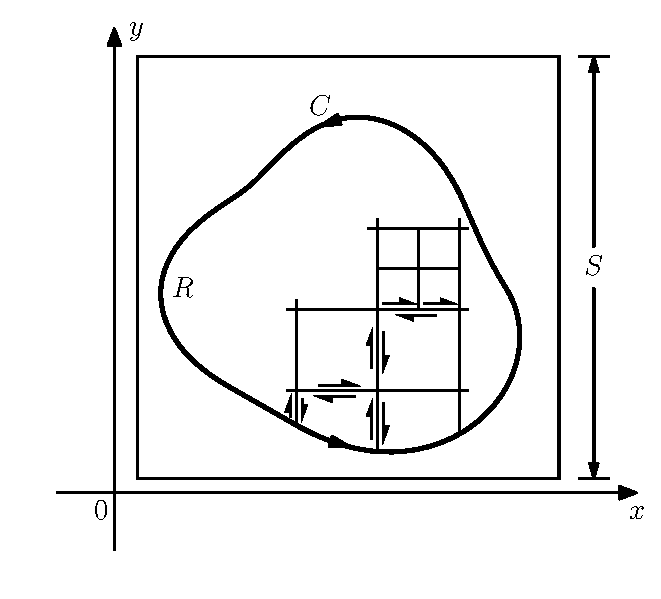
\includegraphics[width=\textwidth]{figuras/cauchy_goursat_lemma_contours.pdf}
  \end{minipage}\hfill
  \begin{minipage}[c]{0.4\textwidth}
    \caption{
       Las integrales sobre segmentos de regiones adyacentes se cancelan.
    }\label{fig:cauchy_goursat_lemma_contours}
  \end{minipage}
\end{figure}

\subsection*{Conclusión}

Para finalizar, se empleará el teorema de la sección \ref{sec:upper_bounds_for_moduli_of_contour_integrals} para encontrar una cota superior para cada módulo en la derecha de la ecuación \ref{eq:cauchy_goursat_theorem_integral_bound}. Para hacerlo, se recuerda que cada \(C_j\) consiste en la frontera de un cuadrado o cuadrado parcial. En cualquier caso, sea \(s_j\) el largo de un lado del cuadrado. Observando que en la integral \(j\)-ésima tanto la variable \(z\) como el punto \(z_j\) pertenecen al cuadrado,
\[
 |z-z_j|\leq\sqrt{2}s_j,
\]
esto es, la distancia entre dos puntos cualesquiera pertenecientes al cuadrado no supera el largo de la diagonal. Por lo tanto, de la ecuación \ref{eq:cauchy_goursat_theorem_deltaj_bound} se deduce que cada integrando en el lado derecho de la ecuación \ref{eq:cauchy_goursat_theorem_integral_bound} satisface la condición
\[
 |(z-z_j)\delta_j|=|z-z_j||\delta_j|<\sqrt{2}s_j\epsilon
\]
Además, el largo del camino \(C_j\) es \(4s_j\) si \(C_j\) es la frontera de un cuadrado. En ese caso, de la ecuación \ref{eq:contour_integral_upper_bound},
\begin{equation}\label{eq:cauchy_goursat_theorem_bound_complete}
 \left|\int_{C_j}(z-z_j)\delta_j(z)\,dz\right|<\sqrt{2}s_j\epsilon4s_j=4\sqrt{2}A_j\epsilon, 
\end{equation}
donde \(A_j=s^2_j\) es el área del cuadrado. En el caso en que \(C_j\) es la frontera de un cuadrado parcial, su longitud no supera \(4s_j+L_j\), donde \(L_j\) es el largo de la parte de \(C_j\) que también es parte de \(C\). Nuevamente denominando \(A_j\) al área del cuadrado completo, se cumple que 
\begin{equation}\label{eq:cauchy_goursat_theorem_bound_partial}
 \left|\int_{C_j}(z-z_j)\delta_j(z)\,dz\right|<\sqrt{2}s_j\epsilon(4s_j+L_j)=4\sqrt{2}s_j^2\epsilon+\sqrt{2}s_jL_j\epsilon<4\sqrt{2}A_j\epsilon+\sqrt{2}SL_j\epsilon, 
\end{equation}
donde \(S\) es la longitud del lado de algún cuadrado que encierra completamente al contorno \(C\) así como a todos los cuadrados empleados inicialmente para cubrir a la región \(R\), como se muestra en la figura \ref{fig:cauchy_goursat_lemma_contours}. Observar que la suma de todos los \(A_j\) no excede a \(S^2\).

Combinando las ecuaciones \ref{eq:cauchy_goursat_theorem_integral_bound}, \ref{eq:cauchy_goursat_theorem_bound_complete} y \ref{eq:cauchy_goursat_theorem_bound_partial} se tiene que 
\begin{align*}
 \left|\int_Cf(z)\,dz\right|&\leq\sum_{j=1}^n\left|\int_{C_j}(z-z_j)\delta_j(z)\,dz\right|\\
  &\overset{(a)}{<}\sum_{j_k}4\sqrt{2}A_{j_k}\epsilon+\sum_{j_l}\left(4\sqrt{2}A_{j_l}\epsilon+\sqrt{2}SL_{j_l}\epsilon\right)\\
  &\overset{(b)}{=}4\sqrt{2}\epsilon\sum_{j=1}^{n}A_j+\sqrt{2}S\epsilon\sum_{j_k}L_j,
\end{align*}
donde en \((a)\) la primera sumatoria tiene \(n_1\) términos correspondientes a todos los cuadrados completos y la segunda sumatoria contiene \(n_2\) términos correspondientes a todos los cuadrados parciales que cubren a la región \(R\), y se cumple que \(n_1+n_2=n\), que es el número total de cuadrados y cuadrados parciales, y en \((b)\) se combinaron las dos sumatorias que tienen como términos las áreas \(A_j\). Finalmente, considerando que la suma de todos los \(A_j\) no excede a \(S^2\) y la suma de todos los \(L_j\) es la longitud total \(L\) del contorno \(C\), resulta en que 
\[
 \left|\int_Cf(z)\,dz\right|<\left(4\sqrt{2}S^2+\sqrt{2}SL\right)\epsilon.
\]
Como el valor del número positivo \(\epsilon\) es arbitrario puede ser elegido tal que el lado derecho de la desigualdad sea tan pequeño como se desee. Por lo tanto, el lado izquierdo, que es independiente de \(\epsilon\), debe ser cero, resultando en la afirmación \ref{eq:cauchy_goursat_theorem}. Esto completa la prueba del teorema de Cauchy-Goursat.

\section{Dominios simplemente conectados}\label{sec:simply_connected_domains}

Un dominio \(D\) se dice \emph{simplemente conectado} o \emph{simplemente conexo} si cada contorno cerrado simple contenido en el encierra únicamente puntos de \(D\). Un ejemplo es el conjunto de puntos interiores a un contorno cerrado simple. El dominio anular entre dos círculos concéntricos no es simplemente conectado. Los dominios que no son simplemente conectados se discuten en la próxima sección.

No es necesario que el contorno cerrado en el teorema de Cauchy-Goursat sea simple cuando el teorema es adaptado a dominios simplemente conectados. Mas precisamente, el contorno puede en realidad cruzarse a si mismo. El siguiente teorema permite esta posibilidad.

\paragraph{Teorema.} Si una función \(f\) es analítica en un dominio \(D\) simplemente conectado, se cumple que 
\begin{equation}\label{eq:cauchy_goursat_theorem_simply_conected_extension}
 \int_Cf(z)\,dz=0 
\end{equation}
para todo contorno \(C\) cerrado contenido en \(D\).

La prueba es fácil cuando \(C\) es un contorno cerrado simple o es un contorno cerrado que se intersecta a si mismo una cantidad \emph{finita} de veces. Si \(C\) es simple y está contenido en \(D\), \(f\) es analítica en los puntos interiores y sobre \(C\), por lo que se aplica el teorema de Cauchy-Goursat y se cumple la ecuación \ref{eq:cauchy_goursat_theorem_simply_conected_extension}. Si \(C\) es cerrado pero se intersecta a si mismo una cantidad finita de veces, puede descomponerse en una cantidad finita de contornos cerrados simples y nuevamente puede aplicarse el teorema de Cauchy-Goursat. Esto se ilustra en la figura \ref{fig:cauchy_goursat_theorem_not_simple_extension}, donde se construyen dos contornos cerrados simples \(C_1\) y \(C_2\) a partir de \(C\). Como los valores de las integrales sobre \(C_1\) y \(C_2\) son cero independientemente de la orientación, se cumple que 
\[
 \int_Cf(z)\,dz=\int_{C_1}f(z)\,dz+\int_{C_2}f(z)\,dz=0.
\]
\begin{figure}[!htb]
  \begin{minipage}[c]{0.42\textwidth}
    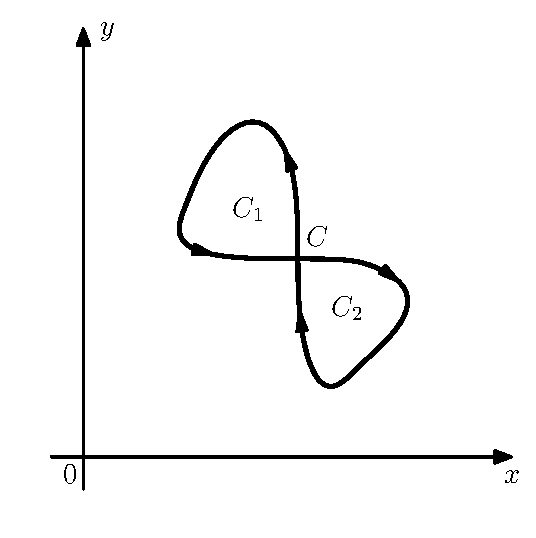
\includegraphics[width=\textwidth]{figuras/cauchy_goursat_theorem_not_simple_extension.pdf}
  \end{minipage}\hfill
  \begin{minipage}[c]{0.48\textwidth}
    \caption{
        Un contorno cerrado que se intersecta a si mismo puede descomponerse en contornos cerrados simples.
    }\label{fig:cauchy_goursat_theorem_not_simple_extension}
  \end{minipage}
\end{figure}

En el caso en que el contorno se intersecta a si mismo una cantidad infinita de veces surgen algunas sutilezas. Un método que en ocasiones puede emplearse para mostrar que el teorema continúa siendo válido se ilustra en el ejercicio 5 de la sección \ref{sec:multiply_connected_domains}.

\paragraph{Corolario 1.} Una función \(f\) que es analítica en un dominio \(D\) simplemente conectado debe tener primitiva en todos lados en \(D\).

Para la prueba, se observa que si la función es analítica en \(D\) debe ser continua allí. Por hipótesis del corolario, la ecuación \ref{eq:cauchy_goursat_theorem_simply_conected_extension} se cumple para todo contorno cerrado \(C\) en \(D\), y por el teorema de la sección \ref{sec:antiderivatives}, \(f\) tiene primitiva en \(D\). 

\paragraph{Corolario 2.} Las funciones completas siempre tienen primitivas.

Este corolario es consecuencia inmediata del Corolario 1 y del hecho de que el plano complejo finito es simplemente conectado.

\section{Dominios múltiplemente conectados}\label{sec:multiply_connected_domains}

Un dominio que no es simplemente conectado se dice \emph{múltiplemente conectado} o \emph{múltiplemente conexo}. El siguiente teorema es una adaptación del teorema de Cauchy-Goursat para dominios múltiplemente conectados. Si bien la hipótesis del teorema involucra \(n\) contornos etiquetados como \(C_k\), con \(k=1,\,2,\,\dots,\,n\), la prueba será guiada por la figura \ref{fig:cauchy_goursat_theorem_multiply_connected}, en donde \(n=2\).

\paragraph{Teorema.} Supóngase que 
\begin{enumerate}
 \item[(\textit{a})] \(C\) es un contorno cerrado simple con orientación antihoraria;
 \item[(\textit{b})] \(C_k\), con \(k=1,\,2,\,\dots,\,n\), son contornos cerrados simples interiores a \(C\), todos con orientación horaria, que son disjuntos y cuyos interiores no tienen puntos en común, como se muestra en la figura \ref{fig:cauchy_goursat_theorem_multiply_connected}.
\end{enumerate}
Si una función \(f\) es analítica sobre dichos contornos y en los puntos interiores a \(C\) y exteriores a cada \(C_k\), se cumple que 
\begin{equation}\label{eq:cauchy_goursat_theorem_multiply_conected_extension}
 \int_Cf(z)\,dz+\sum_{k=1}^n\int_{C_k}f(z)\,dz=0. 
\end{equation}

Notar que en la ecuación \ref{eq:cauchy_goursat_theorem_multiply_conected_extension}, la dirección de cada camino de integración es tal que el dominio múltiplemente conectado se encuentra a la izquierda de los caminos.

\begin{figure}[!htb]
  \begin{minipage}[c]{0.6\textwidth}
    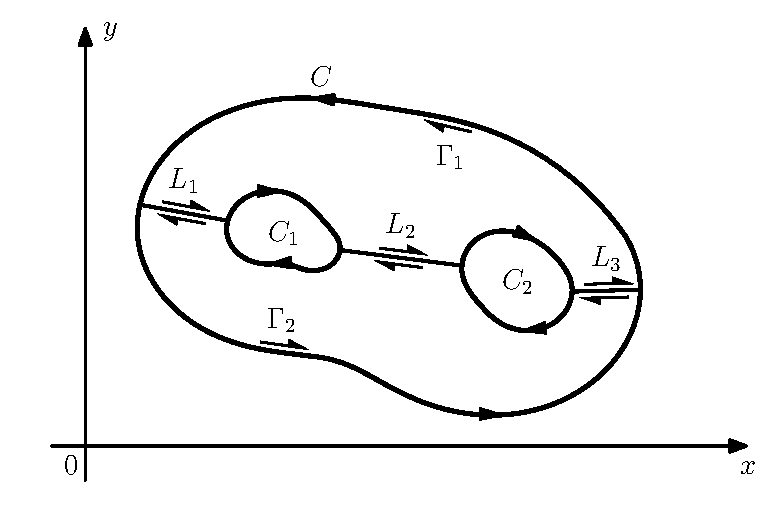
\includegraphics[width=\textwidth]{figuras/cauchy_goursat_theorem_multiply_connected.pdf}
  \end{minipage}\hfill
  \begin{minipage}[c]{0.3\textwidth}
    \caption{
       Contornos empleados en la demostración de la extensión del teorema de Cauchy-Goursat para dominios múltiplemente conectados. 
    }\label{fig:cauchy_goursat_theorem_multiply_connected}
  \end{minipage}
\end{figure}
Para probar el teorema, se introduce un camino poligonal \(L_1\), que consiste en en número finito de segmentos unidos extremo por los extremos que conecta el contorno exterior \(C\) con el contorno interior \(C_1\). Se introduce otro camino poligonal \(L_2\) que conecta a \(C_1\) con \(C_2\), y se continúa de esa forma, con \(L_{n+1}\) conectando a \(C_n\) con \(C\). Como se muestra en la figura \ref{fig:cauchy_goursat_theorem_multiply_connected}, se forman dos contornos cerrados simples \(\Gamma_1\) y \(\Gamma_2\) que consisten en los caminos poligonales \(L_k\) o \(-L_k\) y partes de \(C\) y \(C_k\), y con orientación tal que los puntos que encierran cada uno se encuentran a la izquierda. El teorema de Cauchy-Goursat puede aplicarse a \(f\) sobre los caminos \(\Gamma_1\) y \(\Gamma_2\), y la suma de dichas integrales sobre esos contornos es cero. Como las integrales en direcciones opuestas sobre cada camino poligonal \(L_k\) se cancelan, solo permanecen las integrales sobre \(C\) y \(C_k\), y se obtiene el resultado de la ecuación \ref{eq:cauchy_goursat_theorem_multiply_conected_extension}.

\paragraph{Corolario.} Sean \(C_1\) y \(C_2\) contornos cerrados simples orientados positivamente, donde \(C_1\) es interior a \(C_2\), como se muestra en la figura \ref{fig:cauchy_goursat_deformation_principle}. Si una función \(f\) es analítica en la región cerrada que consiste en dichos contornos y todos los puntos entre ellos, se cumple que 
\begin{equation}\label{eq:cauchy_goursat_principle_of_deformation_of_paths}
 \int_{C_1}f(z)\,dz=\int_{C_2}f(z)\,dz. 
\end{equation}

\begin{figure}[!htb]
  \begin{minipage}[c]{0.6\textwidth}
    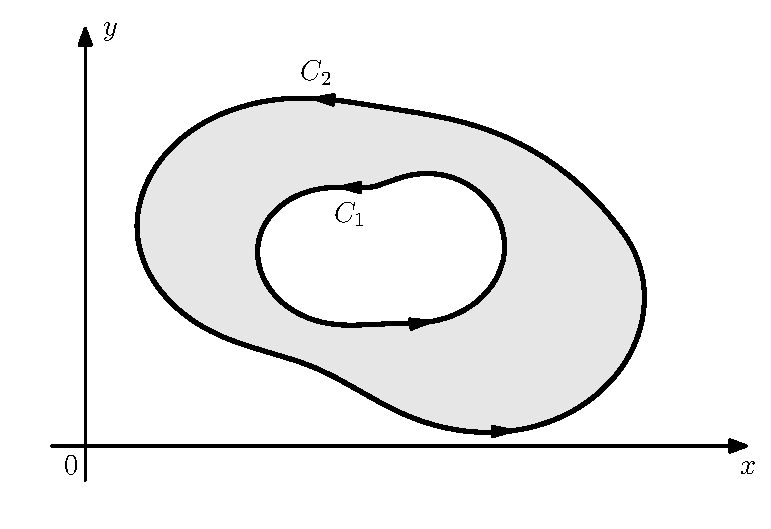
\includegraphics[width=\textwidth]{figuras/cauchy_goursat_deformation_principle.pdf}
  \end{minipage}\hfill
  \begin{minipage}[c]{0.3\textwidth}
    \caption{
       Principio de deformación de caminos. 
    }\label{fig:cauchy_goursat_deformation_principle}
  \end{minipage}
\end{figure}
Este corolario se conoce como \emph{principio de deformación de caminos}, ya que indica que si el contorno \(C_1\) es continuamente deformado a \(C_2\) siempre pasando por puntos en donde \(f\) es analítica, el valor de la integral de \(f\) sobre \(C_1\) no cambia. Para verificar el corolario, alcanza con observar que del teorema se cumple que 
\[
 \int_{C_2}f(z)\,dz+\int_{-C_1}f(z)\,dz=0,
\]
que es lo mismo que la ecuación \ref{eq:cauchy_goursat_principle_of_deformation_of_paths}.

\subsection*{Ejercicios}

\subsubsection*{Ejercicio 1}

Aplicar el teorema de Cauchy-Goursat para mostrar que 
\[
 \int_Cf(z)\,dz=0
\]
cuando el contorno \(C\) es el círculo unidad \(|z|=1\) con cualquier orientación, y cuando
\[
 \begin{array}{lll}
  (\textit{a})\;f(z)=\dfrac{z^2}{z+3};\qquad\qquad\qquad\qquad&(\textit{b})\;f(z)=ze^{-z};\qquad\qquad\qquad\qquad
  (\textit{c})\;f(z)=\dfrac{1}{z^2+2z+2};\\[\bigskipamount]
  (\textit{d})\;f(z)=\sech z;\qquad\qquad\qquad\qquad&(\textit{e})\;f(z)=\tan z;\qquad\qquad\qquad\qquad
  (\textit{f})\;f(z)=\Log(z+2).
 \end{array}
\]

\paragraph{Solución.} 
\begin{enumerate}
 \item[(\textit{a})] La función tiene una singularidad en \(z=-3\), y como es un punto exterior a \(C\), es analítica en \(C\) y en los puntos interiores a \(C\). Como \(C\) es un contorno cerrado simple, se cumplen las hipótesis del teorema de Cauchy-Goursat por lo que la integral vale cero.
 \item[(\textit{b})] La función es analítica en todo el plano complejo por lo que del teorema de Cauchy-Goursat, la integral sobre \(C\) vale cero.
 \item[(\textit{c})] La función tiene puntos singulares en las raíces del denominador, que son
 \[
  \frac{-2\pm\sqrt{4-8}}{2}=\frac{-2\pm2i}{2}=-1\pm i.
 \]
 Como se muestra en la figura \ref{fig:exercise_53_01_f}, las singularidades son exteriores al círculo unidad, y del teorema de Cauchy-Goursat, la integral sobre \(C\) vale cero.
 \item[(\textit{d})] La función
 \[
  f(z)=\sech z=\frac{1}{\cosh z}
 \]
 tiene singularidades en los puntos donde \(\cosh z=0\). Del teorema de la sección \ref{sec:hyperbolic_functions}, esos puntos son
 \[
  z=\left(\frac{\pi}{2}+n\pi\right)i
  \qquad\textrm{con}\qquad 
  n=0,\,\pm1,\,\pm2,\,\dots.
 \]
 Como todas las singularidades son exteriores al círculo unidad, del teorema de Cauchy-Goursat, la integral sobre \(C\) vale cero. Ver la figura \ref{fig:exercise_53_01_f}.
 \item[(\textit{e})] La función
 \[
  f(z)=\tan z=\frac{\sin z}{\cos z}
 \]
 tiene singularidades en los puntos donde \(\cos z=0\). Del teorema de la sección  \ref{sec:zeros_singularities_trigonometric}, esos puntos son
 \[
  z=\frac{\pi}{2}+n\pi
  \qquad\textrm{con}\qquad 
  n=0,\,\pm1,\,\pm2,\,\dots,
 \]
 exteriores al círculo unidad (ver la figura \ref{fig:exercise_53_01_f}). Del teorema de Cauchy-Goursat, la integral sobre \(C\) vale cero.
 \item[(\textit{f})] La función \(\Log(z+2)\) es analítica en todo el pano complejo excepto en el corte de rama, dado por \(|z+2|>0,\,-\pi<\Arg(z+2)<\pi\), que consiste en el punto \(z=-2\) y la semirrecta \(y=0,\,x<-2\) (ver el ejercicio 10 de la sección \ref{sec:logarithm_branches}). Como el corte de rama es exterior al círculo unidad, como se muestra en la figura \ref{fig:exercise_53_01_f}, la integral sobre el contorno \(C\) es cero.
\end{enumerate}
\begin{figure}[!htb]
  \begin{minipage}[c]{0.65\textwidth}
    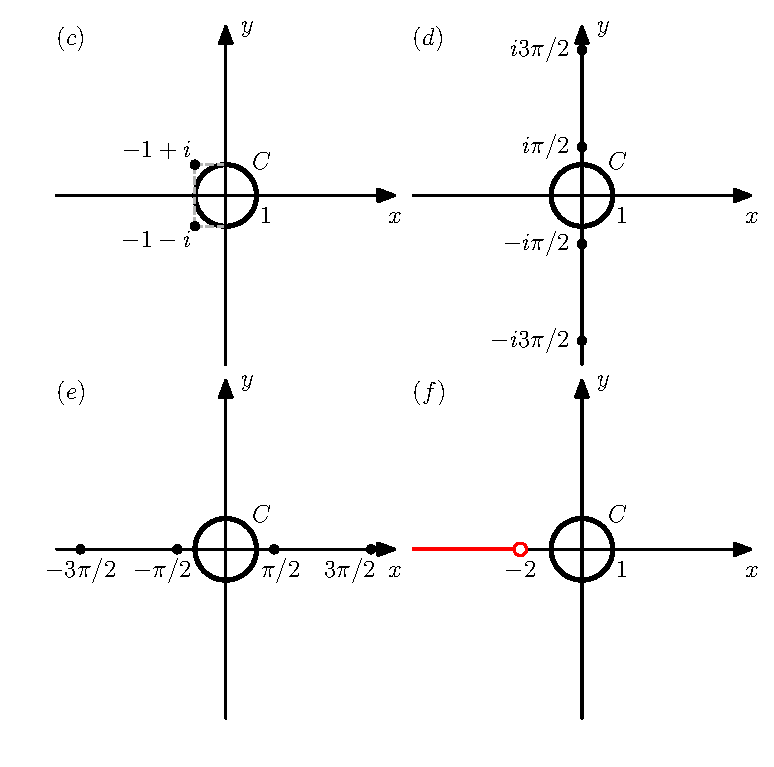
\includegraphics[width=\textwidth]{figuras/exercise_53_01_f.pdf}
  \end{minipage}\hfill
  \begin{minipage}[c]{0.25\textwidth}
    \caption{
       Singularidades de las funciones del ejercicio 1. En todos los casos las singularidades son exteriores al círculo \(|z|\leq1\).
    } \label{fig:exercise_53_01_f}
  \end{minipage}
\end{figure}

\subsubsection*{Ejercicio 2}

Sea \(C_1\) la frontera orientada positivamente del cuadrado cuyos lados se encuentran sobre las rectas \(x=\pm1,\,y=\pm1\) y sea \(C_2\) el círculo \(|z|=4\) orientado positivamente, como se muestra en la figura \ref{fig:exercise_53_02}. Con la ayuda del corolario de la sección \ref{sec:multiply_connected_domains} indicar porque
\[
 \int_{C_1}f(z)\,dz=\int_{C_2}f(z)\,dz
\]
cuando
\[
 (\textit{a})\;f(z)=\frac{1}{3z^2+1};\qquad\qquad (\textit{b})\;f(z)=\frac{z+2}{\sen(z/2)};\qquad\qquad (\textit{c})\;f(z)=\frac{z}{1-e^z}.
\]
\begin{figure}[!htb]
  \begin{minipage}[c]{0.48\textwidth}
    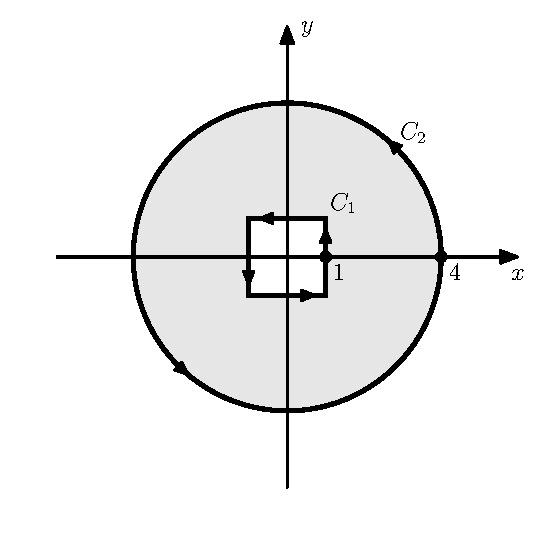
\includegraphics[width=\textwidth]{figuras/exercise_53_02.pdf}
  \end{minipage}\hfill
  \begin{minipage}[c]{0.42\textwidth}
    \caption{
       Contornos \(C_1\) y \(C_2\) involucrados en el ejercicio 2.
    }\label{fig:exercise_53_02}
  \end{minipage}
\end{figure}

\paragraph{Solución.} 
\begin{enumerate}
 \item[(\textit{a})] Los puntos singulares de la función son aquellos en donde el denominador se anula, es decir,
 \[
  3z^2+1=0
  \qquad\qquad\Leftrightarrow\qquad\qquad
  z^2=-\frac{1}{3}
  \qquad\qquad\Leftrightarrow\qquad\qquad
  z=\pm\frac{i}{\sqrt{3}}.
 \]
 Como las singularidades son interiores a \(C_1\), la función es analítica sobre \(C_1\), \(C_2\) y los puntos entre \(C_1\) y \(C_2\), por lo que del corolario de la sección \ref{sec:multiply_connected_domains}, se cumple la ecuación \ref{eq:cauchy_goursat_principle_of_deformation_of_paths}.
 \item[(\textit{b})] Las singularidades de la función son los puntos donde \(\sen(z/2)=0\), dados por (ver el teorema de la sección \ref{sec:zeros_singularities_trigonometric})
 \[
  \sen(z/2)=0
  \qquad\Leftrightarrow\qquad
  \frac{z}{2}=n\pi
  \qquad\Leftrightarrow\qquad
  z=2n\pi,
  \qquad\textrm{con}\qquad 
  n=0,\,\pm1,\,\pm2,\,\dots.
 \]
 Se observa que la singularidad \(z=0\), que se da en el caso en que \(n=0\), es interior a \(C_1\), y las singularidades \(z=2n\pi\) con \(n=\pm1,\,\pm2,\,\dots\), son exteriores a \(C_2\). Por lo tanto, como la función es analítica sobre los contornos \(C_1\) y \(C_2\) y los puntos entre ellos, se cumple la ecuación \ref{eq:cauchy_goursat_principle_of_deformation_of_paths}.
 \item[(\textit{c})] Nuevamente, las singularidades de la función son los puntos en donde el denominador \(1-e^z=0\). Estos puntos son
 \[
  e^z=1
  \qquad\Leftrightarrow\qquad
  e^xe^{iy}=1e^{2n\pi i}
  \qquad\Leftrightarrow\qquad
  z=2n\pi i
  \qquad\textrm{con}\qquad 
  n=0,\,\pm1,\,\pm2,\,\dots.
 \]
 Se observa que la singularidad \(z=0\) es interior a \(C_1\), y las singularidades \(z=2n\pi i\) con \(n=\pm1,\,\pm2,\,\dots\), son exteriores a \(C_2\), por lo que se cumple la ecuación \ref{eq:cauchy_goursat_principle_of_deformation_of_paths}.
\end{enumerate}

\subsubsection*{Ejercicio 3}

Si \(C_0\) denota el círculo \(|z-z_0|=R\) orientado positivamente, se cumple que
\[
 \int_{C_0}(z-z_0)^{n-1}\,dz=
 \left\{ 
 \begin{array}{ll}
  0 &\textrm{si }n=\pm1,\,\pm2,\,\dots\\
  2\pi i&\textrm{si }n=0,
 \end{array}
 \right.
\]
como se dedujo en el ejercicio 13 de la sección \ref{sec:integrals_examples_with_branch_cuts}. 
Emplear dicho resultado junto con el corolario de la sección \ref{sec:multiply_connected_domains} para mostrar que si \(C\) es la frontera del rectángulo \(0\leq x\leq3\), \(0\leq y\leq2\) descripta en sentido positivo, se cumple que 
\[
 \int_{C}(z-2-i)^{n-1}\,dz=
 \left\{ 
 \begin{array}{ll}
  0 &\textrm{si }n=\pm1,\,\pm2,\,\dots\\
  2\pi i&\textrm{si }n=0.
 \end{array}
 \right.
\]

\paragraph{Solución.} La función \(f(z)=(z-z_0)^{n-1}\) es analítica en todo el plano complejo excepto en el punto \(z=z_0\) cuando \(n\leq0\). Si \(C_0\) es el círculo \(|z-z_0|=R\) de centro \(z_0=2+i\) y radio \(R<1\), del ejercicio 13 de la sección \ref{sec:integrals_examples_with_branch_cuts}
\[
 \int_{C_0}(z-2-i)^{n-1}\,dz=
 \left\{ 
 \begin{array}{ll}
  0 &\textrm{si }n=\pm1,\,\pm2,\,\dots\\
  2\pi i&\textrm{si }n=0,
 \end{array}
 \right.
\]
y \(C_0\) es interior al rectángulo \(C\), como se muestra en la figura \ref{fig:exercise_53_03}.
\begin{figure}[!htb]
 \begin{center}
 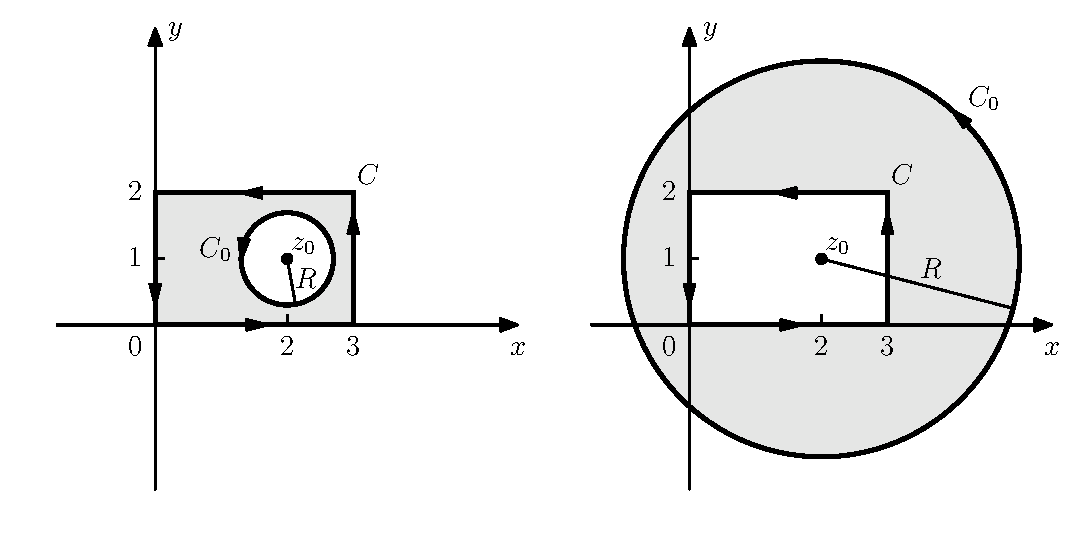
\includegraphics[width=0.85\textwidth]{figuras/exercise_53_03.pdf}
 \caption{\label{fig:exercise_53_03} Contornos \(C_0\) y \(C\) empleados en el ejercicio 3.}
 \end{center}
\end{figure}
De esta forma, la función es analítica sobre los contornos \(C_0\) y \(C\) y los puntos entre ellos. Por lo tanto, del corolario de la sección \ref{sec:multiply_connected_domains},
\[
 \int_{C}(z-2-i)^{n-1}\,dz=\int_{C_0}(z-2-i)^{n-1}\,dz,
\]
obteniendo el resultado buscado.

Observar que se podría haber elegido el círculo \(C_0\) con radio \(R>\sqrt{5}\), como se muestra en la figura  \ref{fig:exercise_53_03}. De esa forma, el rectángulo \(C\) está contenido en el círculo \(C_0\) y la función es analítica sobre los contornos \(C_0\) y \(C\) y los puntos entre ellos, y del corolario se obtiene el mismo resultado.

\subsubsection*{Ejercicio 4}

Emplear el siguiente método para derivar la fórmula de integración
\[
 \int_0^\infty e^{-x^2}\cos 2bx\,dx=\frac{\sqrt{\pi}}{2}e^{-b^2},
 \qquad\qquad b>0. 
\]
\begin{enumerate}
 \item[(\textit{a})] Mostrar que la suma de las integrales de \(e^{-z}\) sobre los lados horizontales inferior y superior del camino rectangular de la figura \ref{fig:exercise_53_04} puede escribirse como
 \[
  2\int_0^2e^{-x^2}\,dx-2e^{b^2}\int_0^2e^{-x^2}\cos2bx\,dx
 \]
 y la suma de las integrales sobre los lados verticales de la izquierda y la derecha se puede escribir como
 \[
  ie^{-a^2}\int_0^be^{y^2}e^{-i2ay}\,dy-ie^{-a^2}\int_0^be^{y^2}e^{i2ay}\,dy.
 \]
 De esta forma, con la ayuda del teorema de Cauchy-Goursat, mostrar que 
 \[
  \int_0^ae^{-x^2}\cos2bx\,dx=e^{-b^2}\int_0^ae^{-x^2}\,dx+e^{-(a^2+b^2)}\int_0^be^{y^2}\sen2ay\,dy.
 \]
 \begin{figure}[!htb]
  \begin{minipage}[c]{0.40\textwidth}
    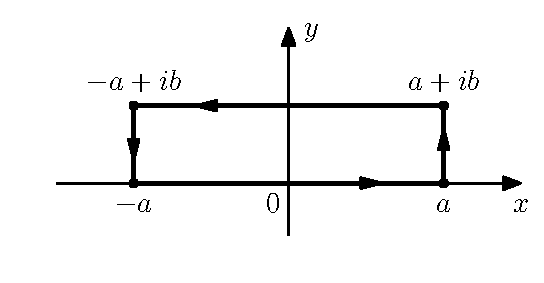
\includegraphics[width=\textwidth]{figuras/exercise_53_04.pdf}
  \end{minipage}\hfill
  \begin{minipage}[c]{0.50\textwidth}
    \caption{
        Contorno empleado en el ejercicio 4.
    }\label{fig:exercise_53_04}
  \end{minipage}
\end{figure}
 \item[(\textit{b})] Aceptando el hecho de que\footnote{Ver \url{https://en.wikipedia.org/wiki/Gaussian_integral}, por ejemplo.} 
 \[
  \int_0^\infty e^{-x^2}\,dx=\frac{\sqrt{\pi}}{2}
 \]
 y observando que 
 \[
  \left|\int_0^be^{y^2}\sen2ay\,dy\right|\leq\int_0^be^{y^2}\,dy
 \]
 obtener la fórmula de integración deseada haciendo que \(a\) tienda a infinito en la última ecuación de la parte (\textit{a}).
\end{enumerate}

\paragraph{Solución}

\begin{enumerate}
 \item[(\textit{a})] Sea \(C_1\) el lado horizontal inferior en el sentido indicado en la figura \ref{fig:exercise_53_04}. Considerando que \(C_1\) se puede parametrizar como \(z=x+i0\) con \(-a\leq x\leq a\),
 \[
  \int_{C_1}e^{-z^2}\,dz=\int_{-a}^a e^{-x^2}\,dx=2\int_0^ae^{-x^2}\,dx.
 \]
 Siendo \(C_3\) el lado horizontal superior en el sentido indicado en la figura \ref{fig:exercise_53_04}, \(-C_3\) se puede parametrizar como \(z=x+bi\)  con \(-a\leq x\leq a\). Por lo tanto,
 \begin{align*}
   \int_{C_3}e^{-z^2}\,dz&=-\int_{-C_3}e^{-z^2}\,dz\\
    &=-\int_{-a}^a e^{-(x+bi)^2}\,dx\\
    &=-\int_{-a}^a e^{-(x^2-b^2+2xbi)}\,dx\\
    &=-e^{b^2}\int_{-a}^a e^{-x^2}e^{-2xbi}\,dx\\
    &=-e^{b^2}\left(\int_0^a e^{-x^2}e^{-2xbi}\,dx+\int_{-a}^0 e^{-x^2}e^{-2xbi}\,dx\right)\\
    &=-e^{b^2}\left(\int_0^a e^{-x^2}e^{-2xbi}\,dx-\int_{a}^0 e^{-u^2}e^{2ubi}\,du\right)\\
    &=-e^{b^2}\left(\int_0^a e^{-x^2}e^{-2xbi}\,dx+\int_0^a e^{-x^2}e^{2xbi}\,dx\right)\\
    &=-e^{b^2}\int_0^a e^{-x^2}\left(e^{2xbi}+e^{-2xbi}\right)\,dx\\
    &=-2e^{b^2}\int_0^a e^{-x^2}\cos 2xb\,dx.
 \end{align*}
 Combinando los resultados, resulta en
 \[
  \int_{C_1}e^{-z^2}\,dz+\int_{C_3}e^{-z^2}\,dz=2\int_0^ae^{-x^2}\,dx-2e^{b^2}\int_0^a e^{-x^2}\cos 2xb\,dx.
 \]
 Siendo \(C_2\) el lado vertical derecho, \(z(y)=a+iy\) con \(0\leq y\leq b\). Observando que \(z'(y)=i\), se tiene que 
 \begin{align*}
  \int_{C_2}e^{-z^2}\,dz&=\int_0^b e^{-(a+iy)^2}i\,dy\\
    &=i\int_0^b e^{-(a^2-y^2+2ayi)}\,dy\\
    &=ie^{-a^2}\int_0^b e^{y^2}e^{-2ayi}\,dy.
 \end{align*}
 Siendo \(C_4\) el lado vertical derecho en el sentido indicado en la figura, \(-C_4\) se puede parametrizar como \(z=-a+iy\) con \(0\leq y\leq b\). Por lo tanto,
 \begin{align*}
   \int_{C_4}e^{-z^2}\,dz&=-\int_{-C_4}e^{-z^2}\,dz\\
    &=-\int_0^b e^{-(-a+iy)^2}i\,dy\\
    &=-i\int_0^b e^{-(a^2-y^2-2ayi)}\,dy\\
    &=-ie^{-a^2}\int_0^b e^{y^2}e^{2ayi}\,dy.
 \end{align*}
 Combinando los resultados, se ve que
 \begin{align*}
  \int_{C_2}e^{-z^2}\,dz+\int_{C_4}e^{-z^2}\,dz&=ie^{-a^2}\int_0^b e^{y^2}e^{-2ayi}\,dy-ie^{-a^2}\int_0^b e^{y^2}e^{2ayi}\,dy\\
   &=ie^{-a^2}\int_0^b e^{y^2}\left(e^{-2ayi}-e^{2ayi}\right)\,dy\\
   &=2e^{-a^2}\int_0^b e^{y^2}\left(\frac{e^{2ayi}-e^{-2ayi}}{2i}\right)\,dy\\
   &=2e^{-a^2}\int_0^b e^{y^2}\sen2ay\,dy.
 \end{align*}
 Considerando que la función \(e^{-z^2}\) es completa, del teorema de Cauchy-Goursat, se cumple que 
 \[
  \int_{C_1+C_2+C_3+C_4}e^{-z^2}\,dz=0,
 \]
 por lo que combinando los resultados obtenidos previamente,
 \[
  2\int_0^ae^{-x^2}\,dx-2e^{b^2}\int_0^a e^{-x^2}\cos 2xb\,dx+2e^{-a^2}\int_0^b e^{y^2}\sen2ay\,dy=0,
 \]
 es decir,
 \[
  e^{b^2}\int_0^a e^{-x^2}\cos 2xb\,dx=\int_0^ae^{-x^2}\,dx+e^{-a^2}\int_0^b e^{y^2}\sen2ay\,dy,
 \]
 resultando en 
 \begin{equation}\label{eq:exercise_53_04}
  \int_0^a e^{-x^2}\cos 2xb\,dx=e^{-b^2}\int_0^ae^{-x^2}\,dx+e^{-(a^2+b^2)}\int_0^b e^{y^2}\sen2ay\,dy,  
 \end{equation}
 que es lo que se quería mostrar.
 \item[(\textit{b})] Observando que 
 \[
  \left|\int_0^b e^{y^2}\sen2ay\,dy\right|\leq\int_0^b\left|e^{y^2}\sen2ay\right|\,dy\leq\int_0^b e^{y^2}\,dy
 \]
 y por lo tanto 
 \[
  \lim_{a\to\infty}\left|e^{-(a^2+b^2)}\int_0^b e^{y^2}\sen2ay\,dy\right|\leq\lim_{a\to\infty}e^{-(a^2+b^2)}\int_0^b e^{y^2}\,dy=0,
 \]
 tomando el límite cuando \(a\) tiende a infinito en la ecuación \ref{eq:exercise_53_04}, se obtiene que 
 \[
  \int_0^\infty e^{-x^2}\cos 2xb\,dx=e^{-b^2}\int_0^\infty e^{-x^2}\,dx=\frac{\sqrt{\pi}}{2}e^{-b^2},
 \]
 que es lo que se quería mostrar.
\end{enumerate}

\subsubsection*{Ejercicio 5}

De acuerdo al ejercicio 6 de la sección \ref{sec:contours}, el camino \(C_1\) desde el origen hasta el punto \(z=1\) sobre la gráfica de la función
\[
 y(x)=\left\{ 
 \begin{array}{ll}
  x^3\sen(\pi/x)&\textrm{cuando }0<x\leq1\\
  0&\textrm{cuando }x=0.
 \end{array}
 \right.
\]
es un arco suave que intersecta al eje real un número infinito de veces. Sea \(C_2\) el segmento sobre el eje real desde \(z=1\) hasta el origen, y sea \(C_3\) cualquier arco suave desde el origen hasta \(z=1\) que no se intersecta a si mismo y solo tiene los puntos extremos en común con \(C_1\) y \(C_2\), como se muestra en la figura \ref{fig:exercise_53_05}. Aplicar el teorema de Cauchy-Goursat para mostrar que si una función \(f\) es completa,
\[
 \int_{C_1}f(z)\,dz=\int_{C_3}f(z)\,dz
 \qquad\qquad\textrm{y}\qquad\qquad
 \int_{C_2}f(z)\,dz=-\int_{C_3}f(z)\,dz.
\]
Concluir que aunque el contorno cerrado \(C=C_1+C_2\) se intersecta a si mismo una cantidad infinita de veces, se sigue cumpliendo que 
\[
 \int_{C}f(z)\,dz=0.
\]
\begin{figure}[!htb]
 \begin{minipage}[c]{0.56\textwidth}
  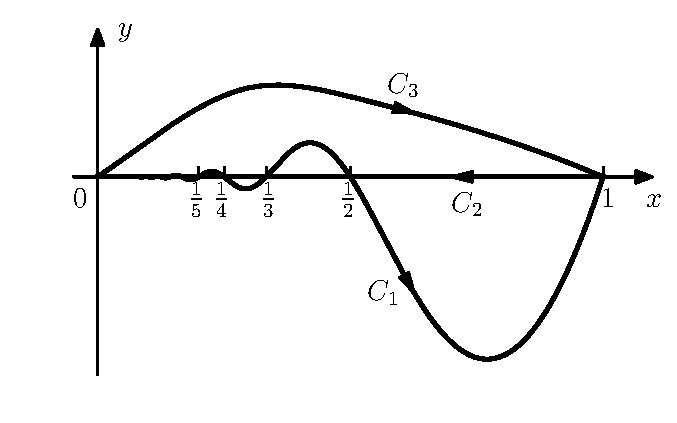
\includegraphics[width=\textwidth]{figuras/exercise_53_05.pdf}
 \end{minipage}\hfill
 \begin{minipage}[c]{0.34\textwidth}
    \caption{
       Contornos \(C_1\), \(C_2\) y \(C_3\) involucrados en el ejercicio 5.
    }\label{fig:exercise_53_05}
 \end{minipage}
\end{figure}

\paragraph{Solución.} El contorno \(C_1-C_3\) es cerrado simple, y como \(f\) es completa, del teorema de Cauchy-Goursat se cumple que 
\[
 \int_{C_1-C_3}f(z)\,dz=\int_{C_1}f(z)\,dz-\int_{C_3}f(z)\,dz=0
\]
y por lo tanto,
\[
 \int_{C_1}f(z)\,dz=\int_{C_3}f(z)\,dz
\]
Empleando el mismo argumento con el contorno \(C_2+C_3\),
\[
 \int_{C_2+C_3}f(z)\,dz=\int_{C_2}f(z)\,dz+\int_{C_3}f(z)\,dz=0
\]
y por lo tanto,
\[
 \int_{C_2}f(z)\,dz=-\int_{C_3}f(z)\,dz.
\]
Combinando los resultados, se obtiene que 
\[
 \int_{C_1}f(z)\,dz=-\int_{C_2}f(z)\,dz
 \qquad\qquad\Leftrightarrow\qquad\qquad 
 \int_{C_1}f(z)\,dz+\int_{C_2}f(z)\,dz=0,
\]
concluyendo que sobre el contorno \(C=C_1+C_2\) que se intersecta a si mismo infinitas veces, se sigue cumpliendo que 
\[
 \int_{C}f(z)\,dz=\int_{C_1+C_2}f(z)\,dz=0.
\]

\subsubsection*{Ejercicio 6}

Sea \(C\) la frontera del medio disco \(0\leq r\leq 1,\, 0\leq\theta\leq\pi\) orientada positivamente, y sea \(f(z)\) la función continua definida en ese medio disco como \(f(0)=0\) y la rama
\[
 f(z)=\sqrt{r}e^{i\theta/2},
 \qquad\qquad
 r>0,\,-\frac{\pi}{2}<\theta<\frac{3\pi}{2}
\]
de la función multivaluada \(z^{1/2}\). Mostrar que 
\[
 \int_Cf(z)\,dz=0
\]
evaluando separadamente las integrales de \(f(z)\) sobre el semicírculo y los dos radios que conforman a \(C\). ¿Porqué el teorema de Cauchy-Goursat no se aplica en este caso?

\paragraph{Solución.} Sea \(C_1\) el semicírculo, \(C_2\) el radio sobre el eje real negativo y \(C_3\) el radio sobre el eje real positivo de \(C\). De esta forma, \(C=C_1+C_2+C_3\).
\begin{itemize}
 \item Sobre \(C_1:\,z=e^{i\theta}\) con \(0\leq\theta\leq\pi\), la integral es
 \begin{align*}
  \int_{C_1}f(z)\,dz&=\int_0^\pi\sqrt{1}e^{i\theta/2}ie^{i\theta}\,d\theta\\
   &=i\int_0^\pi e^{i3\theta/2}\,d\theta\\
   &=i \frac{2}{3i}e^{i3\theta/2}\bigg|_0^\pi\\
   &=\frac{2}{3}\left(e^{i3\pi/2}-1\right)\\
   &=-\frac{2}{3}(1+i).
 \end{align*}
 \item Con \(-C_2:\,z=re^{i\pi}\) con \(0\leq r\leq1\), la integral sobre \(C_2\) es
 \begin{align*}
  \int_{C_2}f(z)\,dz&=-\int_{-C_2}f(z)\,dz\\
   &=-\int_0^1\sqrt{r}e^{i\pi/2}e^{i\pi}\,dr\\
   &=i\int_0^1\sqrt{r}\,dr\\
   &=i\frac{2}{3}r^{3/2}\bigg|_0^1\\
   &=\frac{2}{3}i.
 \end{align*}
 \item Sobre \(C_3:\,z=re^{i0}=r\) con \(0\leq r\leq1\), la integral es
 \begin{align*}
  \int_{C_2}f(z)\,dz&=\int_0^1\sqrt{r}\,dr\\
   &=\frac{2}{3}r^{3/2}\bigg|_0^1\\
   &=\frac{2}{3}.
 \end{align*}
\end{itemize}
Combinando los resultados, se concluye que 
\[
 \int_{C}f(z)\,dz=\int_{C_1}f(z)\,dz+\int_{C_2}f(z)\,dz+\int_{C_3}f(z)\,dz=-\frac{2}{3}(1+i)+\frac{2}{3}i+\frac{2}{3}=0.
\]

En este caso, no se puede aplicar el teorema de Cauchy-Goursat debido a que \(f(z)\) no es analítica en el origen.

\subsubsection*{Ejercicio 7}

Mostrar que si \(C\) es un contorno cerrado simple orientado positivamente, el área de la región encerrada por \(C\) puede calcularse como
\[
 \frac{1}{2i}\int_C\overline{z}\,dz.
\]

\emph{Sugerencia: } notar que puede emplearse la expresión \ref{eq:cauchy_goursat_theorem_contour_integral_with_green_theorem} aunque la función \(f(z)=\overline{z}\) no es analítica en ningún lugar.

\paragraph{Solución.} Se empleará la ecuación \ref{eq:cauchy_goursat_theorem_contour_integral_with_green_theorem} con
\[
 f(z)=\overline{z}=x-iy.
\]
Las funciones componentes de \(f(z)\) son
\[
 u(x,\,y)=x
 \qquad\qquad\textrm{y}\qquad\qquad
 u(x,\,y)=-y,
\]
y sus derivadas parciales son
\[
 \begin{array}{ll}
  u_x(x,\,y)=1\qquad\qquad\qquad\qquad&u_y(x,\,y)=0\\[\smallskipamount]
  v_x(x,\,y)=0\qquad\qquad\qquad\qquad&v_y(x,\,y)=-1.
 \end{array}
\] 
Sustituyendo estos resultados en la ecuación \ref{eq:cauchy_goursat_theorem_contour_integral_with_green_theorem}, se tiene que 
\begin{align*}
 \frac{1}{2i}\int_C \overline{z}\,dz&=\frac{1}{2i}\left(\iint_R0\,dA+i\iint_R2\,dA\right)\\
   &=\frac{1}{2i}\left(0+2i\iint_R\,dA\right)\\
   &=\iint_R\,dA,
\end{align*}
que es lo que se quería mostrar. Observar que la ecuación \ref{eq:cauchy_goursat_theorem_contour_integral_with_green_theorem} surge del teorema de Green (ver la sección \ref{sec:cauchy_goursat_theorem}), que requiere que las funciones componentes \(u(x,\,y)\) y \(u(x,\,y)\) tengan derivadas parciales continuas. Si bien la función \(f(z)=\overline{z}\) no es analítica en ningún lado (ver el ejercicio 1 de la sección \ref{sec:cauchy_riemann_equations_polar}), sus funciones componentes \(u=x\) y \(v=-y\) tienen derivadas de primer orden continuas, por lo que se puede aplicar el teorema de Green.

\subsubsection*{Ejercicio 8}

\emph{Intervalos anidados.} Una secuencia infinita de intervalos cerrados \(a_n\leq x\leq b_n\) con \(n=0,\,1,\,2,\,\dots\) se construye de la siguiente forma. El intervalo \(a_1\leq x\leq b_1\) es tanto la mitad izquierda o la mitad derecha del intervalo \(a_0\leq x\leq b_0\), y el intervalo \(a_2\leq x\leq b_2\) es alguna de las dos mitades de \(a_1\leq x\leq b_1\), y así sucesivamente. Probar que hay un punto \(x_0\) que pertenece a cada uno de los intervalos cerrados \(a_n\leq x\leq b_n\).

\emph{Sugerencia:} notar que los puntos \(a_n\) de la izquierda de los intervalos representan una secuencia no decreciente de números, ya que \(a_0\leq a_n\leq a_{n-1}<b_0\), y por lo tanto, tienen un límite \(A\) cuando \(n\) tiende a infinito. Mostrar que los extremos \(b_n\) también tienen un límite \(B\). Luego mostrar que \(A=B\) y por lo tanto, \(x_0=A=B\).

\paragraph{Solución.} Por construcción, los extremos \(a_n\) de la izquierda de los intervalos cumplen que \(a_0\leq a_n\leq a_{n-1}<b_0\). Esto indica que consisten en una secuencia no decreciente acotada superiormente, y por lo tanto, tienen un límite\footnote{Ver por ejemplo \url{https://en.wikipedia.org/wiki/Monotone_convergence_theorem}.} \(A\),
\[
 \lim_{n\to\infty}a_n=A.
\]
Por otro lado, los extremos \(b_n\) de la derecha cumplen que \(b_0\geq b_{n}\geq b_{n+1}>a_0\), lo que implica que se tratan de una secuencia no creciente acotada inferiormente, y por lo tanto, convergen a un límite \(B\),
\[
 \lim_{n\to\infty}b_n=B.
\]
Además, para todo \(n\) se cumple que 
\[
 b_{n+1}-a_{n+1}=\frac{1}{2}(b_n-a_n)
\]
y por lo tanto,
\[
 \lim_{n\to\infty}(b_n-a_n)=0
 \qquad\qquad\Leftrightarrow\qquad\qquad
 \lim_{n\to\infty}a_n=\lim_{n\to\infty}b_n,
\]
es decir, \(A=B\). Como para todo \(n\) se cumple que \(a_n\leq A=B\leq b_n\), existe un punto \(x_0=A=B\) que pertenece a todos los intervalos.

\subsubsection*{Ejercicio 9}

\emph{Cuadrados anidados.} Un cuadrado \(\sigma_0\,:\,a_0\leq x\leq b_0,\,c_0\leq y\leq d_0\) es dividido en cuatro cuadrados iguales mediante segmentos paralelos a los ejes de coordenadas. Uno de esos cuatro cuadrados \(\sigma_1\,:\,a_1\leq x\leq b_1,\,c_1\leq x\leq d_1\) es seleccionado mediante alguna regla. Éste también es dividido en cuatro cuadrados iguales, uno de los cuales, llamado \(\sigma_2\), es seleccionado, y así sucesivamente (ver la sección \ref{sec:cauchy_goursat_theorem_proof}). Probar que hay un punto \((x_0,\,y_0)\) que pertenece a cada una de las regiones cerradas de la secuencia infinita \(\sigma_0,\,\sigma_1,\,\sigma_2,\,\dots\).

\emph{Sugerencia:} aplicar el resultado del ejercicio 8 a cada una de las secuencias \(a_n\leq x\leq b_n\) y \(c_n\leq y\leq d_n\) con \(n=0,\,1,\,2,\,\dots\).

\paragraph{Solución.} Dividir al cuadrado \(\sigma_n\) en cuatro cuadrados iguales mediante segmentos paralelos a los ejes de coordenadas y seleccionar uno de ellos es equivalente a dividir al segmento horizontal \(a_n\leq x\leq b_n\) a la mitad y seleccionar la mitad izquierda o derecha y dividir al segmento vertical \(c_n\leq y\leq d_n\) a la mitad y seleccionar la mitad inferior o superior. Por lo tanto, en el proceso se obtienen dos secuencias \(a_n\leq x\leq b_n\) y \(c_n\leq y\leq d_n\) con \(n=0,\,1,\,2,\,\dots\) con las mismas características de los intervalos anidados del ejercicio 8. Como se dedujo en dicho ejercicio, existe un punto \(x_0\) que pertenece a cada uno de los intervalos \(a_n\leq x\leq b_n\) y un punto \(y_0\) que pertenece a cada uno de los intervalos \(c_n\leq y\leq d_n\). Por lo tanto, el punto \((x_0,\,y_0)\) pertenece cada uno de los cuadrados \(\sigma_n\,:\,a_n\leq x\leq b_n,\,c_n\leq y\leq d_n\) con \(n=0,\,1,\,2,\,\dots\).

\section{Fórmula integral de Cauchy}\label{sec:cauchy_integral_formula}

Se establecerá a continuación otro resultado fundamental.

\paragraph{Teorema.} Sea \(f\) analítica en todos lados dentro y sobre un contorno \(C\) cerrado simple con orientación positiva. Si \(z_0\) es cualquier punto interior a \(C\), entonces
\begin{equation}\label{eq:cauchy_integral_formula}
 f(z_0)=\frac{1}{2\pi i}\int_C\frac{f(z)}{z-z_0}\,dz. 
\end{equation}

La ecuación \ref{eq:cauchy_integral_formula} se llama \emph{fórmula integral de Cauchy}. Indica que si una función \(f\) es analítica dentro y sobre un contorno \(C\) cerrado simple, los valores de \(f\) interiores a \(C\) quedan completamente determinados por los valores de \(f\) sobre \(C\).

Se comienza la prueba del teorema definiendo a \(C_\rho\) como el círculo \(|z-z_0|=\rho\) orientado positivamente, con \(\rho\) suficientemente pequeño de forma de que \(C_\rho\) sea interior a \(C\), como se muestra en la figura \ref{fig:cauchy_integral_formula}. 
\begin{figure}[!htb]
  \begin{minipage}[c]{0.6\textwidth}
    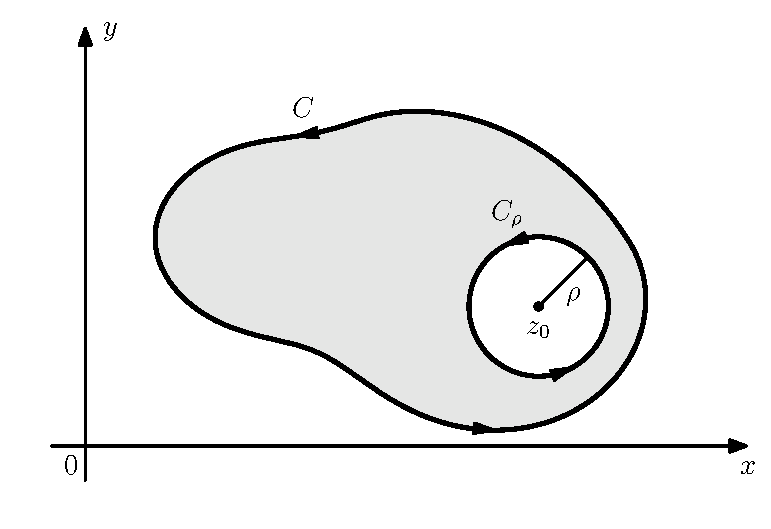
\includegraphics[width=\textwidth]{figuras/cauchy_integral_formula.pdf}
  \end{minipage}\hfill
  \begin{minipage}[c]{0.3\textwidth}
    \caption{
       Contorno \(C_\rho\) empleado en la deducción de la fórmula integral de Cauchy. 
    }\label{fig:cauchy_integral_formula}
  \end{minipage}
\end{figure}
Como el cociente \(f(z)/(z-z_0)\) es analítico entre y sobre los contornos \(C_\rho\) y \(C\), del principio de deformación de caminos (ver la sección \ref{sec:multiply_connected_domains}), se cumple que 
\[
 \int_C\frac{f(z)}{z-z_0}\,dz=\int_{C_\rho}\frac{f(z)}{z-z_0}\,dz.
\]
De esto surge la identidad
\[
 \int_C\frac{f(z)}{z-z_0}\,dz-f(z_0)\int_{C_\rho}\frac{1}{z-z_0}\,dz=\int_{C_\rho}\frac{f(z)-f(z_0)}{z-z_0}\,dz,
\]
y como 
\[
 \int_{C_\rho}\frac{1}{z-z_0}\,dz=2\pi i,
\]
como se obtuvo en el ejercicio 13 de la sección \ref{sec:integrals_examples_with_branch_cuts}, resulta en que  
\begin{equation}\label{eq:cauchy_integral_formula_deduction_tmp}
 \int_C\frac{f(z)}{z-z_0}\,dz-2\pi if(z_0)=\int_{C_\rho}\frac{f(z)-f(z_0)}{z-z_0}\,dz, 
\end{equation}

Ahora, el hecho de que \(f\) sea analítica y por lo tanto continua en \(z_0\), asegura que para todo número \(\epsilon\) positivo existe un número \(\delta\) positivo tal que
\[
 |f(z)-f(z_0)|<\epsilon
 \qquad\textrm{si se cumple que}\qquad
 |z-z_0|<\delta.
\]
Sea el radio \(\rho\) de \(C_\rho\) menor que el número \(\delta\) de la segunda inecuación. Como \(|z-z_0|=\rho<\delta\) cuando \(z\) está sobre \(C_\rho\), la primera inecuación se cumple para los puntos \(z\) sobre \(C_\rho\), y por lo tanto, para dichos puntos
\[
 \left|\frac{f(z)-f(z_0)}{z-z_0}\right|<\frac{\epsilon}{\rho}.
\]
Del teorema de la sección \ref{sec:upper_bounds_for_moduli_of_contour_integrals} de la cota superior del módulo de integrales de contorno, se obtiene que 
\[
 \left|\int_{C_\rho}\frac{f(z)-f(z_0)}{z-z_0}\,dz\right|<\frac{\epsilon}{\rho}2\pi\rho=2\pi\epsilon,
\]
y sustituyendo este resultado en la ecuación \ref{eq:cauchy_integral_formula_deduction_tmp}, resulta en que 
\[
 \left|\int_C\frac{f(z)}{z-z_0}\,dz-2\pi if(z_0)\right|<2\pi\epsilon.
\]
Como el lado derecho de la inecuación es una constante no negativa menor a un número arbitrariamente pequeño, se concluye que 
\[
 \int_C\frac{f(z)}{z-z_0}\,dz-2\pi if(z_0)=0.
\]
Por lo tanto, la ecuación \ref{eq:cauchy_integral_formula} es válida y el teorema queda probado.

Cuando la fórmula integral de Cauchy se expresa como
\[
 \int_C\frac{f(z)}{z-z_0}\,dz=2\pi if(z_0)
\]
puede emplearse para calcular ciertas integrales sobre contornos cerrados simples.

\section{Una extensión de la fórmula integral de Cauchy}\label{sec:cauchy_integral_formula_extension}

La fórmula integral de Cauchy en el teorema de la sección \ref{sec:cauchy_integral_formula} puede extenderse para proveer la representación integral de las derivadas \(f^{(n)}(z_0)\) de \(f\) en \(z_0\).

\paragraph{Teorema.} Sea \(f\) analítica dentro y sobre un contorno cerrado simple \(C\) orientado en sentido positivo. Si \(z_0\) es un punto interior a \(C\), entonces
\begin{equation}\label{eq:cauchy_integral_formula_extension}
 f^{(n)}(z_0)=\frac{n!}{2\pi i}\int_{C}\frac{f(z)}{(z-z_0)^{n+1}}\,dz,
 \qquad\qquad 
 n=0,\,1,\,2,\,\dots. 
\end{equation}

Acordando que 
\[
 f^{(n)}(z_0)=f(z_0)
 \qquad\qquad\textrm{y}\qquad\qquad
 0!=1
\]
el teorema incluye la fórmula integral de Cauchy \ref{eq:cauchy_integral_formula}. La verificación de la ecuación \ref{eq:cauchy_integral_formula_extension} se hará en la sección \ref{sec:cauchy_integral_formula_extension_verification}.

Cuando la ecuación \ref{eq:cauchy_integral_formula_extension} se escribe como 
\[
 \int_{C}\frac{f(z)}{(z-z_0)^{n+1}}\,dz=\frac{2\pi i}{n!}f^{(n)}(z_0)
 \qquad\qquad 
 n=0,\,1,\,2,\,\dots,
\]
puede ser útil para evaluar cierto tipo de integrales cuando \(f\) es analítica dentro y sobre un contorno cerrado simple \(C\) orientado positivamente, y \(z_0\) es un punto interior a \(C\).

Es útil expresar la ecuación \ref{eq:cauchy_integral_formula_extension} en una notación ligeramente diferente. Concretamente, si \(s\) denota a los puntos sobre \(C\) y si \(z\) es un punto interior a \(C\), entonces
\begin{equation}\label{eq:cauchy_integral_formula_extension_alt}
 f^{(n)}(z)=\frac{n!}{2\pi i}\int_{C}\frac{f(s)}{(s-z)^{n+1}}\,ds,
 \qquad\qquad 
 n=0,\,1,\,2,\,\dots. 
\end{equation}

\paragraph{Ejemplo.} Si \(n\) es un entero no negativo y \(f(z)=(z^2-1)^n\), la ecuación \ref{eq:cauchy_integral_formula_extension_alt} queda
\[
 \frac{d^n}{dz^2}(z^2-1)^n=\frac{n!}{2\pi i}\int_{C}\frac{(s^2-1)^n}{(s-z)^{n+1}}\,ds,
 \qquad\qquad 
 n=0,\,1,\,2,\,\dots,
\]
donde \(C\) es cualquier contorno cerrado simple que rodea al punto \(z\). A partir de esta ecuación, los polinomios de Legendre, definidos como (ver el ejercicio 10 de la sección \ref{sec:differentiation_rules})
\[
 P_n(z)=\frac{1}{n!2^n}\frac{d^n}{dz^n}(z^2-1)^n,
 \qquad\qquad n=0,\,1,\,2,\,\dots,
\]
se pueden expresar como
\begin{equation}\label{eq:legendre_polynomials_integral}
 P_n(z)=\frac{1}{2^{n+1}\pi i}\int_{C}\frac{(s^2-1)^n}{(s-z)^{n+1}}\,ds,
 \qquad\qquad 
 n=0,\,1,\,2,\,\dots. 
\end{equation}
Con \(z=1\), el integrando es
\[
 \frac{(s^2-1)^n}{(s-1)^{n+1}}=\frac{(s-1)^n(s+1)^n}{(s-1)^{n+1}}=\frac{(s+1)^n}{s-1}
\]
y la ecuación \ref{eq:legendre_polynomials_integral} queda 
\[
  P_n(1)=\frac{1}{2^{n+1}\pi i}\int_{C}\frac{(s+1)^n}{s-1}\,ds,
 \qquad\qquad 
 n=0,\,1,\,2,\,\dots. 
\]
De la ecuación \ref{eq:cauchy_integral_formula} de la fórmula integral de Cauchy con \(f(z)=(z+1)^n\) y \(z_0=1\)
\[
 \int_C\frac{(z+1)^n}{z-1}\,dz=2\pi i(1+1)^n=2^{n+1}\pi i,
\]
y sustituyendo en la ecuación resulta en que 
\[
 P_n(1)=1.
\]
Los valores \(P_n(-1)=(-1)^n\), \(n=0,\,1,\,2,\,\dots\) pueden obtenerse de forma similar, como se hace en el ejercicio 8 de la sección \ref{sec:cauchy_integral_formula_extension_verification}.

Finalmente, se sugiere a continuación como se obtiene la ecuación \ref{eq:cauchy_integral_formula_extension_alt}. Si \(s\) denota a los puntos sobre la curva \(C\) y \(z\) es un punto interior a \(C\), la fórmula integral de Cauchy es
\[
 f(z)=\frac{1}{2\pi i}\int_{C}\frac{f(s)}{s-z}\,ds,
 \qquad\qquad 
 n=0,\,1,\,2,\,\dots. 
\]
Mediante la diferenciación bajo el signo de integral, sin realizar una justificación rigurosa, se obtiene que 
\[
 f'(z)=\frac{1}{2\pi i}\int_{C}f(s)\frac{\partial}{\partial z}(s-z)^{-1}\,ds
 =\frac{1}{2\pi i}\int_{C}\frac{f(s)}{(s-z)^2}\,ds.
\]
De forma similar,
\[
 f''(z)=\frac{2\times1}{2\pi i}\int_{C}\frac{f(s)}{(s-z)^{2+1}}\,ds
\]
y
\[
 f'''(z)=\frac{3\times2\times1}{2\pi i}\int_{C}\frac{f(s)}{(s-z)^{3+1}}\,ds.
\]

\section{Verificación de la extensión}\label{sec:cauchy_integral_formula_extension_verification}

A continuación se verificará la extensión de la fórmula integral de Cauchy introducida en la sección \ref{sec:cauchy_integral_formula_extension}. Sea \(f\) una función analítica dentro y sobre un contorno \(C\) cerrado simple orientado positivamente, y sea \(z\) cualquier punto interior a \(C\). De la ecuación \ref{eq:cauchy_integral_formula} de la fórmula integral de Cauchy,
\begin{equation}\label{eq:cauchy_integral_formula_extension_deduction_cauchy}
 f(z)=\frac{1}{2\pi i}\int_C\frac{f(s)}{s-z}\,ds. 
\end{equation}

Para verificar que \(f'(z)\) existe y que la expresión 
\begin{equation}\label{eq:cauchy_integral_formula_extension_first_derivative}
 f'(z)=\frac{1}{2\pi i}\int_C\frac{f(s)}{(s-z)^2}\,ds, 
\end{equation}
obtenida en la sección \ref{sec:cauchy_integral_formula_extension} es válida, llámese \(d\) a la menor distancia entre \(z\) y los puntos \(s\) en \(C\), y asúmase que \(0<|\Delta z|<d\), como se muestra en la figura \ref{fig:cauchy_integral_formula_extension}. 
\begin{figure}[!htb]
  \begin{minipage}[c]{0.6\textwidth}
    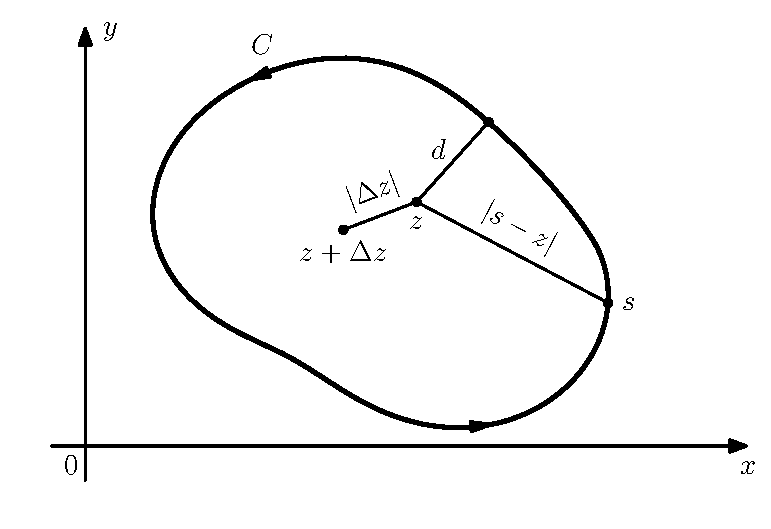
\includegraphics[width=\textwidth]{figuras/cauchy_integral_formula_extension.pdf}
  \end{minipage}\hfill
  \begin{minipage}[c]{0.3\textwidth}
    \caption{
       Contorno \(C\) y puntos involucrados en la deducción de la extensión de la fórmula integral de Cauchy. 
    }\label{fig:cauchy_integral_formula_extension}
  \end{minipage}
\end{figure}
De la ecuación \ref{eq:cauchy_integral_formula_extension_deduction_cauchy}, se tiene que 
\[
 \frac{f(z+\Delta z)-f(z)}{\Delta z}=\frac{1}{2\pi i}\int_C\left(\frac{1}{s-z-\Delta z}-\frac{1}{s-z}\right)\frac{f(s)}{\Delta z}\,ds,
\]
y sacando denominador común en el integrando, se obtiene que 
\[
 \frac{f(z+\Delta z)-f(z)}{\Delta z}=\frac{1}{2\pi i}\int_C\frac{f(s)}{(s-z-\Delta z)(s-z)}\,ds.
\]
Considerando que 
\[
 \frac{1}{(s-z-\Delta z)(s-z)}=\frac{1}{(s-z)^2}+\frac{\Delta z}{(s-z-\Delta z)(s-z)^2},
\]
se llega a que 
\begin{equation}\label{eq:cauchy_integral_formula_extension_deduction_difference_quotient}
 \frac{f(z+\Delta z)-f(z)}{\Delta z}-\frac{1}{2\pi i}\int_C\frac{f(s)}{(s-z)^2}\,ds=\frac{1}{2\pi i}\int_C\frac{\Delta zf(s)}{(s-z-\Delta z)(s-z)^2}\,ds. 
\end{equation}

Continuando, sea \(M\) el valor máximo de \(|f(s)|\) sobre \(C\) y observando que \(|s-z|\geq d\) y \(|\Delta z|<d\), se cumple que 
\[
 |s-z-\Delta z|=|(s-z)-\Delta z|\geq||s-z|-|\Delta z||\geq d-|\Delta z|>0.
\]
Por lo tanto, en los puntos \(s\) sobre \(C\), el integrando de la integral en el lado derecho de la ecuación \ref{eq:cauchy_integral_formula_extension_deduction_difference_quotient} cumple que 
\[
 \left|\frac{\Delta zf(s)}{(s-z-\Delta z)(s-z)^2}\right|\leq\frac{|\Delta z|M}{(d-|\Delta z|)d^2}
\]
y si \(L\) es el largo del contorno \(C\), la ecuación \ref{eq:contour_integral_upper_bound} indica que dicha integral cumple que 
\[
 \left|\int_C\frac{\Delta zf(s)}{(s-z-\Delta z)(s-z)^2}\right|\leq\frac{|\Delta z|M}{(d-|\Delta z|)d^2}L\;\xrightarrow[\Delta z\to0]{}\;0.
\]
De esta forma, tomando el límite cuando \(\Delta z\) tiende a cero en la ecuación \ref{eq:cauchy_integral_formula_extension_deduction_difference_quotient}, se obtiene que 
\[
 \lim_{\Delta z\to0}\frac{f(z+\Delta z)-f(z)}{\Delta z}-\frac{1}{2\pi i}\int_C\frac{f(s)}{(s-z)^2}\,ds=0,
\]
que es la expresión deseada para \(f'(z)\).

Empleando la misma técnica puede verificarse la expresión
\[
 f''(z)=\frac{1}{\pi i}\int_{C}\frac{f(s)}{(s-z)^3}\,ds,
\]
como se hace en el ejercicio 9 de esta sección. La ecuación general \ref{eq:cauchy_integral_formula_extension_alt} puede obtenerse mediante inducción matemática, como se hace por ejemplo en la sección 72 de \cite{markushevich1965theory}.

\section{Algunas consecuencias de la extensión}\label{sec:cauchy_integral_formula_extension_consecuences}

En esta sección se mencionan algunas consecuencias importantes de la extensión de la fórmula integral de Cauchy de la sección \ref{sec:cauchy_integral_formula_extension}.

\paragraph{Teorema 1.} Si una función \(f\) es analítica en un punto, sus derivadas de todos los ordenes también son analíticas en ese punto.

Para probar este teorema fundamental, asúmase que una función \(f\) es analítica en un punto \(z_0\). Por lo tanto, debe haber un entorno \(|z-z_0|<\epsilon\) de \(z_0\) en el cual \(f\) es analítica (ver la sección \ref{sec:analytic_functions}). En consecuencia, hay un círculo \(C_0\) de centro \(z_0\) y radio \(\epsilon/2\) orientado positivamente tal que \(f\) es analítica sobre y dentro de \(C_0\). De la ecuación \ref{eq:cauchy_integral_formula_extension_alt}, se sabe que 
\[
 f''(z)=\frac{1}{\pi i}\int_{C_0}\frac{f(s)}{(s-z)^3}\,ds,
\]
en cada punto \(z\) interior a \(C_0\), y la existencia de \(f''(z)\) dentro del entorno \(|z-z_0|<\epsilon/2\) significa que \(f'\) es analítica en \(z_0\). Aplicando el mismo razonamiento a la función analítica \(f'\), se prueba que su derivada \(f''\) es analítica en \(z_0\), y así sucesivamente. Esto concluye la prueba del teorema.

Como consecuencia, cuando una función
\[
 f(z)=u(x,\,y)+iv(x,\,y)
\]
es analítica en el punto \(z=(x,\,y)\), el teorema indica que \(f'\) es diferenciable, y esto asegura la continuidad de \(f'\) en ese punto (ver el final de la sección \ref{sec:derivatives}). Por lo tanto, como (ver la sección \ref{sec:cauchy_riemann_equations})
\[
 f'(z)=u_x+iv_x=v_y-iu_y,
\]
se concluye que las derivadas parciales de primer orden de \(u\) y \(v\) son continuas en ese punto (ver el teorema 3 de la sección \ref{sec:continuity_definition}). Además, como \(f''\) es diferenciable y continua en \(z\) y como
\[
 f''(z)=u_{xx}+iv_{xx}=v_{yx}-iu_{yx},
\]
las derivadas parciales de segundo orden de \(u\) y \(v\) son continuas. Continuando con el mismo razonamiento para las derivadas de mayor orden, se arriba al siguiente corolario, que fue anticipado en la sección \ref{sec:harmonic_functions} sobre las funciones armónicas.

\paragraph{Corolario.} Si una función \(f(z)=u(x,\,y)+iv(x,\,y)\) es analítica en un punto \(z=(x,\,y)\), entonces las funciones componentes \(u\) y \(v\) tienen derivadas parciales de todos los ordenes continuas.

La prueba del siguiente teorema, referido como teorema de Morera\footnote{Ver \href{https://en.wikipedia.org/wiki/Morera\%27s\_theorem}{https://en.wikipedia.org/wiki/Morera's\_theorem}, por ejemplo.} se basa en el hecho de que la derivada de una función analítica es analítica, como indica el teorema 1.

\paragraph{Teorema 2.} Sea una función \(f\) continua en un dominio \(D\). Si
\[
 \int_Cf(z)\,dz=0
\]
para cada contorno cerrado \(C\) en \(D\), entonces \(f\) es analítica en todo \(D\).

En particular, cuando \(D\) es simplemente conectado, el teorema es el recíproco del teorema de la sección \ref{sec:simply_connected_domains} para la clase de funciones continuas definidas en \(D\), que es la adaptación del teorema de Cauchy-Goursat para dichos dominios.

Para probar el teorema 2, se observa que si se satisfacen sus hipótesis, el teorema de la sección \ref{sec:antiderivatives} asegura que \(f\) tiene primitiva en \(D\); es decir, existe una función analítica \(F\) tal que \(F'(z)=f(z)\) en cada punto de \(D\). Como \(f\) es la derivada de \(F\), el teorema 1 indica que \(f\) es analítica en \(D\).

El siguiente último teorema es esencial en la siguiente sección.

\paragraph{Teorema 3.} Supóngase que una función \(f\) es analítica dentro y sobre un círculo \(C_R\) orientado positivamente con centro en \(z_0\) y radio \(R\). Si \(M_R\) denota el máximo valor de \(|f(z)|\) sobre \(C_R\), entonces
\begin{equation}\label{eq:cauchy_inequality}
 |f^{(n)}(z_0)|\leq\frac{n!M_R}{R^n},
 \qquad\qquad 
 n=1,\,2,\,\dots. 
\end{equation}

La ecuación \ref{eq:cauchy_inequality} se llama \emph{desigualdad de Cauchy} y es consecuencia inmediata de la ecuación \ref{eq:cauchy_integral_formula_extension}
\[
 f^{(n)}(z_0)=\frac{n!}{2\pi i}\int_{C}\frac{f(z)}{(z-z_0)^{n+1}}\,dz,
 \qquad\qquad 
 n=1,\,2,\,\dots
\]
cuando \(n\) es un entero positivo. Efectivamente, considerando que el integrando cumple que 
\[
 \left|\frac{f(z)}{(z-z_0)^{n+1}}\right|\leq\frac{M_R}{R^{n+1}}
\]
y el perímetro del círculo es \(2\pi R\), aplicando la ecuación \ref{eq:contour_integral_upper_bound} se obtiene que 
\[
 \left|f^{(n)}(z_0)\right|\leq\frac{n!}{2\pi}\times\frac{M_R}{R^{n+1}}\times2\pi R=\frac{n!M_R}{R^n}.
\]

\subsection*{Ejercicios}

\subsubsection*{Ejercicio 1}

Sea \(C\) la frontera orientada positivamente del cuadrado cuyos lados están en las rectas \(x=\pm2\) y \(y=\pm2\). Evaluar cada una de las siguientes integrales:
\begin{align*}
 (\textit{a})\;&\int_C\frac{e^{-z}}{z-(\pi i/2)}\,dz;\qquad\qquad
 (\textit{b})\;\int_C\frac{\cos z}{z(z^2+8)}\,dz;\qquad\qquad
 (\textit{c})\;\int_C\frac{z}{2z+1}\,dz;\\[\bigskipamount]
 (\textit{d})\;&\int_C\frac{\cosh z}{z^4}\,dz;\qquad\qquad\qquad
 (\textit{d})\;\int_C\frac{\tan(z/2)}{(z-x_0)^2}\,dz\qquad\textrm{con}\qquad 
 -2<x_0<2.
\end{align*}

\paragraph{Solución.} 
\begin{enumerate}
 \item[(\textit{a})] De la ecuación \ref{eq:cauchy_integral_formula} de la fórmula integral de Cauchy con \(f(z)=e^{-z}\)   y \(z_0=i\pi/2\), considerando que \(f(z)\) es completa y \(z_0\) es interior a \(C\),
 \[
  \int_C\frac{e^{-z}}{z-i\pi/2}\,dz=2\pi if(i\pi/2)=2\pi i e^{-i\pi/2}=2\pi i(-i)=2\pi.
 \]
 \item[(\textit{b})] Con \(z_0=0\) interior a \(C\) y 
 \[
  f(z)=\frac{\cos z}{z^2+8}
 \]
 en la ecuación \ref{eq:cauchy_integral_formula}, y teniendo en cuenta que los puntos singulares de \(f(z)\) son \(\pm i2\sqrt{2}\) exteriores a \(C\),
 \[
  \int_C\frac{\cos z}{z(z^2+8)}\,dz=\int_C\frac{f(z)}{z-0}\,dz=2\pi if(0)=2\pi i\frac{\cos0}{8}=\frac{i\pi}{4}.
 \]
 \item[(\textit{c})] Con \(z_0=-1/2\) interior a \(C\) y \(f(z)=z/2\) completa en la ecuación \ref{eq:cauchy_integral_formula},
 \[
  \int_C\frac{z}{2z+1}\,dz=\int_C\frac{z/2}{z+1/2}\,dz=\int_C\frac{f(z)}{z+1/2}\,dz=2\pi if(-1/2)=2\pi i(-1/4)=-\frac{i\pi}{2}.
 \]
 \item[(\textit{d})] Con \(z_0=0\) interior a \(C\), \(f(z)=\cosh z\) completa y \(n=3\) en la ecuación \ref{eq:cauchy_integral_formula_extension} de la extensión de la fórmula integral de Cauchy,
 \[
  \int_C\frac{\cosh z}{z^4}\,dz=\int_C\frac{f(z)}{(z-0)^{3+1}}\,dz=\frac{2\pi i}{3!}f'''(0)\overset{(a)}{=}\frac{\pi i}{3}\senh0=0,
 \]
 donde en \((a)\) se consideró que \((\cosh z)'''=\senh z\) (ver la ecuación \ref{eq:sinh_cosh_derivatives}).
 \item[(\textit{e})] Con \(z_0=x_0\) interior a \(C\) ya que \(-2<x_0<2\), \(f(z)=\tan(z/2)\) y \(n=1\) en la ecuación \ref{eq:cauchy_integral_formula_extension},
 \[
  \int_C\frac{\tan(z/2)}{(z-x_0)^2}\,dz=\int_C\frac{f(z)}{(z-x_0)^{1+1}}\,dz\overset{(a)}{=}2\pi if'(x_0)=\pi i\sec^2\left(\frac{x_0}{2}\right),
 \]
 donde en \((a)\) se consideró que 
 \[
  f'(z)=\frac{1}{2}\sec^2\left(\frac{z}{2}\right),
 \]
 como indica la ecuación \ref{eq:tan_cot_sec_csc_derivatives}.
\end{enumerate}

\subsubsection*{Ejercicio 2}

Encontrar el valor de la integral de \(g(z)\) alrededor del círculo \(|z-i|=2\) orientado positivamente cuando 
\[
 (\textit{a})\;g(z)=\frac{1}{z^2+4};\qquad\qquad 
 (\textit{b})\;g(z)=\frac{1}{(z^2+4)^2}.
\]

\paragraph{Solución}
\begin{enumerate}
 \item[(\textit{a})] Considerando que 
 \[
  g(z)=\frac{1}{z^2+4}=\frac{1}{(z-2i)(z+2i)},
 \]
 y teniendo en cuenta que la singularidad en \(2i\) es interior a \(C\) y la singularidad en \(-2i\) es exterior a \(C\), la función 
 \[
  f(z)=\frac{1}{z+2i}
 \]
 es analítica dentro y sobre \(C\). Por lo tanto, de la ecuación \ref{eq:cauchy_integral_formula} fórmula integral de Cauchy
 \[
  \int_C\frac{1}{z^2+4}\,dz=\int_C\frac{1}{(z-2i)(z+2i)}\,dz=\int_C\frac{f(z)}{z-2i}\,dz=2\pi if(2i)=\frac{2\pi i}{4i}=\frac{\pi}{2}.
 \]
 \item[(\textit{b})] De forma similar, como
 \[
  g(z)=\frac{1}{(z^2+4)^2}=\frac{1}{(z-2i)^2(z+2i)^2},  
 \]
 definiendo la función 
 \[
  f(z)=\frac{1}{(z+2i)^2}
 \]
 analítica sobre y dentro de \(C\), de la extensión de la fórmula integral de Cauchy (ecuación \ref{eq:cauchy_integral_formula_extension}) con \(n=1\),
 \[
  \int_C\frac{1}{(z^2+4)^2}\,dz=\int_C\frac{f(z)}{(z-2i)^2}=2\pi if'(2i)
  \overset{(a)}{=}2\pi i\left[\frac{-2}{(4i)^3}\right]=\frac{-\pi i}{4^2(-i)}=\frac{\pi}{16},
 \]
 donde en \((a)\) se consideró que 
 \[
  f'(z)=\frac{-2}{(z+2i)^3}.
 \]
\end{enumerate}

\subsubsection*{Ejercicio 3}

Sea \(C\) el círculo \(|z|=3\) orientado positivamente. Mostrar que si
\[
 g(z)=\int_C\frac{2s^2-s-2}{s-z}\,ds,
 \qquad\qquad
 |z|\neq3,
\]
entonces \(g(2)=8\pi i\). ¿Cuál es el valor de \(g(z)\) cuando \(|z|>3\)?

\paragraph{Solución.} De la fórmula integral de Cauchy \ref{eq:cauchy_integral_formula} con \(f(s)=2s^2-s-2\), que es completa, y considerando que el punto \(z=2\) es interior a \(C\), se tiene que 
\[
 g(2)=\int_C\frac{2s^2-s-2}{s-2}\,ds=\int_C\frac{f(s)}{s-2}\,ds=2\pi if(2)=8\pi i.
\]
En el caso en que \(|z|>3\), el integrando es analítico sobre y dentro de \(C\), por lo que del teorema de Cauchy-Goursat (ver la sección \ref{sec:cauchy_goursat_theorem}), \(g(z)=0\).

\subsubsection*{Ejercicio 4}

Sea \(C\) un contorno cerrado simple orientado positivamente en el plano \(z\) y sea
\[
 g(z)=\int_C\frac{s^3+2s}{(s-z)^3}\,ds.
\]
Mostrar que \(g(z)=6\pi iz\) cuando \(z\) es interior a \(C\) y \(g(z)=0\) cuando \(z\) es exterior a \(C\).

\paragraph{Solución.} Si \(z\) es interior a \(C\), como el numerador \(f(s)=s^3+2s\) es una función completa, de la extensión \ref{eq:cauchy_integral_formula_extension_alt} de la fórmula integral de Cauchy con \(n=2\),
\[
 g(z)=\int_C\frac{s^3+2s}{(s-z)^3}\,ds=\int_C\frac{f(s)}{(s-z)^{2+1}}\,ds=\frac{2\pi i}{2!}f''(z)\overset{(a)}{=}6\pi iz,
\]
donde en \((a)\) se consideró que \(f'(s)=3s^2+2\) y \(f''(s)=6s\).

Si \(z\) es exterior a \(C\), el integrando es analítico sobre y dentro de \(C\), por lo que del teorema de Cauchy-Goursat, \(g(z)=0\).

\subsubsection*{Ejercicio 5}

Mostrar que si \(f\) es analítica dentro y sobre un contorno \(C\) cerrado simple y \(z_0\) no está sobre \(C\), entonces
\[
 \int_C\frac{f'(z)}{z-z_0}\,dz=\int_C\frac{f(z)}{(z-z_0)^2}\,dz.
\]

\paragraph{Solución.} Como \(f\) es analítica dentro y sobre \(C\), \(f'\) también lo es, como indica el teorema 1 en esta sección. Si el punto \(z_0\) es interior a \(C\), de la fórmula integral de Cauchy \ref{eq:cauchy_integral_formula},
\[
 \int_C\frac{f'(z)}{z-z_0}\,dz=2\pi if'(z_0),
\]
y de la extensión \ref{eq:cauchy_integral_formula_extension} de la fórmula integral de Cauchy con \(n=1\),
\[
 \int_C\frac{f(z)}{(z-z_0)^2}\,dz=2\pi if'(z_0),
\]
resultando en que el valor de las dos integrales es el mismo, como se quería probar.

En el caso en que \(z_0\) es exterior a \(C\), los integrandos de ambas integrales son funciones analíticas dentro y sobre \(C\), por lo que del teorema de Cauchy-Goursat, valen cero.

\subsubsection*{Ejercicio 6}

Sea \(f\) una función que es \emph{continua} sobre un contorno \(C\) cerrado simple. Siguiendo el procedimiento realizado en la sección \ref{sec:cauchy_integral_formula_extension_verification}, probar que la función
\[
 g(z)=\frac{1}{2\pi i}\int_C\frac{f(s)}{s-z}\,ds
\]
es analítica en cada punto \(z\) interior a \(C\) y que 
\[
 g'(z)=\frac{1}{2\pi i}\int_C\frac{f(s)}{(s-z)^2}\,ds
\]
en ese punto.

\paragraph{Solución.} Como \(f\) es continua sobre \(C\) y el punto \(z\) es interior a \(C\), el integrando de
\[
 g(z)=\frac{1}{2\pi i}\int_C\frac{f(s)}{s-z}\,ds
\]
es continuo sobre \(C\) por lo que la función \(g(z)\) está bien definida para todo \(z\) interior a \(C\) (ver la sección \ref{sec:contour_integrals}). Para probar que \(g\) es analítica en el punto \(z\), hay que probar que existe la derivada en \(z\) (ver la sección \ref{sec:analytic_functions}), es decir, que existe el límite
\[
 \lim_{\Delta z\to0}\frac{g(z+\Delta z)-g(z)}{\Delta z}.
\]
Además, hay que probar que el resultado del límite es
\[
 g'(z)=\frac{1}{2\pi i}\int_C\frac{f(s)}{(s-z)^2}\,ds.
\]
Esto se hace siguiendo exactamente el mismo razonamiento que el realizado en la sección \ref{sec:cauchy_integral_formula_extension_verification}.

\subsubsection*{Ejercicio 7}

Sea \(C\) el círculo unidad \(z=e^{i\theta}\) con \(-\pi\leq\theta\leq\pi\). Primero mostrar que para cualquier constante real \(a\),
\[
 \int_C\frac{e^{az}}{z}\,dz=2\pi i.
\]
Luego, escribir esta integral en términos de \(\theta\) para derivar la fórmula de integración
\[
 \int_0^\pi e^{a\cos\theta}\cos(a\sen\theta)\,d\theta=\pi.
\]

\paragraph{Solución.} Con \(f(z)=e^{az}\) completa y \(z_0=0\) interior a \(C\), de la fórmula integral de Cauchy (ecuación \ref{eq:cauchy_integral_formula}) se tiene que 
\begin{equation}\label{eq:exercise_57_07_a}
 \int_C\frac{e^{az}}{z}\,dz=\int_C\frac{f(z)}{z-0}\,dz=2\pi if(0)=2\pi ie^0=2\pi i. 
\end{equation}
Expresando a \(C\) de forma paramétrica como \(z(\theta)=e^{i\theta}\) con \(-\pi\leq\theta\leq\pi\),
\begin{align}
 \int_C\frac{e^{az}}{z}\,dz&\overset{(a)}{=}\int_{-\pi}^\pi\frac{e^{ae^{i\theta}}}{e^{i\theta}}ie^{i\theta}\,d\theta\nonumber\\
  &=i\int_{-\pi}^\pi e^{ae^{i\theta}}\,d\theta\nonumber\\
  &\overset{(b)}{=}i\int_{-\pi}^\pi e^{a\cos\theta}\left[\cos(a\sen\theta)+i\sen(a\sen\theta)\right]\,d\theta\nonumber\\
  &=i\int_{-\pi}^\pi e^{a\cos\theta}\cos(a\sen\theta)\,d\theta-\int_{-\pi}^\pi e^{a\cos\theta}\sen(a\sen\theta)\,d\theta\nonumber\\
  &\overset{(c)}{=}2i\int_{0}^\pi e^{a\cos\theta}\cos(a\sen\theta)\,d\theta,\label{eq:exercise_57_07_b}
\end{align}
donde en \((a)\) se empleó la ecuación \ref{eq:contour_integral_definition} y se consideró que \(z'(\theta)=ie^{i\theta}\), en \((b)\) se tuvo en cuenta que 
\[
 e^{ae^{i\theta}}=e^{a(\cos\theta+i\sen\theta)}=e^{a\cos\theta}e^{ia\sen\theta}=
 e^{a\cos\theta}\left[\cos(a\sen\theta)+i\sen(a\sen\theta)\right],
\]
y en \((c)\) se observó que el integrando de la primera integral es par y por lo tanto la integral es dos veces la integral en la mitad del intervalo de integración, y que el integrando de la segunda integral es impar y por lo tanto vale cero. Para ver la simetría de los integrandos, se observa que el factor \(e^{a\cos\theta}\) es par y que el factor
\[
 \cos[a\sen(-\theta)]=\cos(-a\sen\theta)=\cos(a\sen\theta)
\]
es par y el factor 
\[
 \sen[a\sen(-\theta)]=\sen(-a\sen\theta)=-\sen(a\sen\theta)
\]
es impar. Finalmente, combinando los resultados de las ecuaciones \ref{eq:exercise_57_07_a} y \ref{eq:exercise_57_07_b} se obtiene que 
\[
 \int_{0}^\pi e^{a\cos\theta}\cos(a\sen\theta)\,d\theta=\pi.
\]

\subsubsection*{Ejercicio 8}

Mostrar que \(P_n(-1)=(-1)^n\), \(n=0,\,1,\,2,\,\dots\), donde \(P_n(z)\) son los polinomios de Legendre en el ejemplo de la sección \ref{sec:cauchy_integral_formula_extension}.

\emph{Sugerencia:} Observar que 
\[
 \frac{(s^2-1)^n}{(s+1)^{n+1}}=\frac{(s-1)^n}{s+1}.
\]

\paragraph{Solución.} Los polinomios de Legendre están dados por la ecuación \ref{eq:legendre_polynomials_integral},
\[
 P_n(z)=\frac{1}{2^{n+1}\pi i}\int_{C}\frac{(s^2-1)^n}{(s-z)^{n+1}}\,ds,
 \qquad\qquad 
 n=0,\,1,\,2,\,\dots,
\]
donde \(C\) es cualquier contorno cerrado simple que rodea al punto \(z\). Al evaluar en \(z=-1\), el integrando se puede escribir como
\[
 \frac{(s^2-1)^n}{(s+1)^{n+1}}=\frac{(s+1)^n(s-1)^n}{(s+1)^{n+1}}=\frac{(s-1)^n}{s+1}.
\]
Por lo tanto, con \(f(s)=(s-1)^n\) completa y \(z=-1\) interior a \(C\), aplicando la fórmula integral de Cauchy, se observa que
\[
 P_n(-1)=\frac{1}{2^{n+1}\pi i}\int_{C}\frac{(s-1)^n}{s+1}\,ds=\frac{1}{2^{n+1}\pi i}\int_{C}\frac{f(s)}{s+1}\,ds
 =\frac{1}{2^{n+1}\pi i}2\pi if(-1)=\frac{1}{2^n}(-2)^n=(-1)^n.
\]

\subsubsection*{Ejercicio 9}

Seguir los pasos indicados a continuación para verificar la expresión 
\[
 f''(z)=\frac{1}{\pi i}\int_C\frac{f(s)}{(s-z)^3}\,ds
\]
de la sección \ref{sec:cauchy_integral_formula_extension_verification}.
\begin{enumerate}
 \item[(\textit{a})] Emplear la expresión \ref{eq:cauchy_integral_formula_extension_first_derivative} de \(f'(z)\) para mostrar que 
 \begin{equation}\label{eq:exercise_57_09_tmp2}
  \frac{f'(z+\Delta z)-f'(z)}{\Delta z}-\frac{1}{\pi i}\int_C\frac{f(s)}{(s-z)^3}\,ds
  =\frac{1}{2\pi i}\int_C\frac{3(s-z)\Delta z-2(\Delta z)^2}{(s-z-\Delta z)^2(s-z)^3}f(s)\,ds.
 \end{equation}
 \item[(\textit{b})] Sea \(D\) y \(d\) la distancia mas larga y mas corta respectivamente entre el punto \(z\) y los puntos sobre \(C\). Además, sea \(M\) el valor máximo de \(|f(s)|\) en \(C\) y sea \(L\) el largo de \(C\). Con la ayuda de la desigualdad triangular y la deducción de la ecuación \ref{eq:cauchy_integral_formula_extension_first_derivative} de \(f'(z)\), mostrar que cuando \(0<|\Delta z|<d\), el valor de la integral del lado derecho de la igualdad de la parte (\textit{a}) está acotada superiormente por 
 \[
  \frac{(3D|\Delta z|+2|\Delta z|^2)M}{(d-\Delta z)^2d^3}L.
 \]
 \item[(\textit{c})] Emplear los resultados de las partes (\textit{a}) y (\textit{b}) para obtener la expresión deseada de \(f''(z)\).
\end{enumerate}

\paragraph{Solución.} 
\begin{enumerate}
 \item[(\textit{a})] Partiendo de la expresión \ref{eq:cauchy_integral_formula_extension_first_derivative} de \(f'(z)\),
 \[
  f'(z)=\frac{1}{2\pi i}\int_C\frac{f(s)}{(s-z)^2}\,ds, 
 \]
 se tiene que
 \begin{align*}
  \frac{f'(z+\Delta z)-f'(z)}{\Delta z}&=\frac{1}{2\pi i}\int_C\left[\frac{1}{(s-z-\Delta z)^2}-\frac{1}{(s-z)^2}\right]\frac{f(s)}{\Delta z}\,ds
 \end{align*}
 Desarrollando el término del integrando entre paréntesis rectos, se ve que 
 \begin{align*}
  \frac{1}{(s-z-\Delta z)^2}-\frac{1}{(s-z)^2}&=\frac{(s-z)^2-(s-z-\Delta z)^2}{(s-z-\Delta z)^2(s-z)^2}\\
   &=\frac{(s-z)^2-\left[(s-z)^2-2(s-z)\Delta z+(\Delta z)^2\right]}{(s-z-\Delta z)^2(s-z)^2}\\
   &=\frac{2(s-z)\Delta z-(\Delta z)^2}{(s-z-\Delta z)^2(s-z)^2}
 \end{align*}
 y por lo tanto,
 \begin{equation}\label{eq:exercise_57_09_tmp1}
  \frac{f'(z+\Delta z)-f'(z)}{\Delta z}=\frac{1}{2\pi i}\int_C\frac{2(s-z)-\Delta z}{(s-z-\Delta z)^2(s-z)^2}f(s)\,ds.  
 \end{equation}
 Teniendo en cuenta la igualdad que se quiere demostrar, se observa que 
 \begin{align*}
  \frac{2}{(s-z)^3}+\frac{3(s-z)\Delta z-2(\Delta z)^2}{(s-z-\Delta z)^2(s-z)^3}&=\frac{2(s-z-\Delta z)^2+3(s-z)\Delta z-2(\Delta z)^2}{(s-z-\Delta z)^2(s-z)^3}\\
  &=\frac{2\left[(s-z)^2-2(s-z)\Delta z+(\Delta z)^2\right]+3(s-z)\Delta z-2(\Delta z)^2}{(s-z-\Delta z)^2(s-z)^3}\\
  &=\frac{2(s-z)^2-(s-z)\Delta z}{(s-z-\Delta z)^2(s-z)^3}\\
  &=\frac{2(s-z)-\Delta z}{(s-z-\Delta z)^2(s-z)^2},
 \end{align*}
 que es el término del integrando en la ecuación \ref{eq:exercise_57_09_tmp1}. Reemplazando ese término en la ecuación \ref{eq:exercise_57_09_tmp1} por el lado izquierdo de la igualdad, resulta en que 
 \begin{align*}
  \frac{f'(z+\Delta z)-f'(z)}{\Delta z}&=\frac{1}{2\pi i}\int_C\left[\frac{2}{(s-z)^3}+\frac{3(s-z)\Delta z-2(\Delta z)^2}{(s-z-\Delta z)^2(s-z)^3}\right]f(s)\,ds\\
  &=\frac{1}{\pi i}\int_C\frac{f(s)}{(s-z)^3}\,ds+\frac{1}{2\pi i}\int_C\frac{3(s-z)\Delta z-2(\Delta z)^2}{(s-z-\Delta z)^2(s-z)^3}f(s)\,ds,
 \end{align*}
 que es lo que se quería mostrar. 
 \item[(\textit{b})] Se quiere encontrar una cota superior de la integral del lado derecho de la igualdad de la ecuación \ref{eq:exercise_57_09_tmp2} ,
 \[
  \int_C\frac{3(s-z)\Delta z-2(\Delta z)^2}{(s-z-\Delta z)^2(s-z)^3}f(s)\,ds.
 \]
 Por un lado, para los puntos \(s\) en \(C\), \(|f(s)|\leq M\). Además, el numerador cumple que 
 \[
  |3(s-z)\Delta z-2(\Delta z)^2|\overset{(a)}{\leq}3|s-z||\Delta z|+2|(\Delta z)|^2\overset{(b)}{\leq}3D|\Delta z|+2|\Delta z|^2, 
 \]
 donde en \((a)\) se aplicó al desigualdad triangular y en \((b)\) se consideró que los puntos \(s\) en \(C\) cumplen que \(|s-z|\leq D\). Además, como se mostró en la sección \ref{sec:cauchy_integral_formula_extension_verification}, como
 \[
  |s-z-\Delta z|\geq d-|\Delta z|>0, 
 \]
 el denominador cumple que 
 \[
  |(s-z-\Delta z)^2(s-z)^3|\geq (d-|\Delta z|)^2d^3.
 \]
 Combinando los resultados, el integrando cumple que 
 \[
  \left|\frac{3(s-z)\Delta z-2(\Delta z)^2}{(s-z-\Delta z)^2(s-z)^3}f(s)\right|\leq\frac{3D|\Delta z|+2|\Delta z|^2}{(d-|\Delta z|)^2d^3}M,
 \]
 y teniendo en cuenta que el largo de \(C\) es \(L\), de la ecuación \ref{eq:contour_integral_upper_bound}, se concluye que 
 \[
  \left|\int_C\frac{3(s-z)\Delta z-2(\Delta z)^2}{(s-z-\Delta z)^2(s-z)^3}f(s)\,ds\right|\leq\frac{3D|\Delta z|+2|\Delta z|^2}{(d-|\Delta z|)^2d^3}ML.
 \]
 \item[(\textit{c})] Como
  \[
  \left|\int_C\frac{3(s-z)\Delta z-2(\Delta z)^2}{(s-z-\Delta z)^2(s-z)^3}f(s)\,ds\right|\leq\frac{3D|\Delta z|+2|\Delta z|^2}{(d-|\Delta z|)^2d^3}ML\;\xrightarrow[\Delta z\to0]{}\;0,
 \]
 al tomar el límite de \(\Delta z\) a cero en la ecuación \ref{eq:exercise_57_09_tmp2} se obtiene que 
 \[
  \lim_{\Delta z\to0}\frac{f'(z+\Delta z)-f'(z)}{\Delta z}-\frac{1}{\pi i}\int_C\frac{f(s)}{(s-z)^3}\,ds=0,
 \]
 que es la expresión deseada para \(f''(z)\).
\end{enumerate}

\subsubsection*{Ejercicio 10}

Sea \(f\) una función completa tal que \(f(z)\leq A|z|\) para todo \(z\), donde \(A\) es un número positivo fijo. Mostrar que \(f(z)=a_1z\), donde \(a_1\) es una constante compleja.

\emph{Sugerencia:} emplear la desigualdad de Cauchy (ecuación \ref{eq:cauchy_inequality}) para mostrar que la derivada segunda \(f''(z)\) es cero en todos lados del plano. Notar que la constante \(M_R\) en la desigualdad de Cauchy es menor o igual a \(A(|z_0|+R)\).

\paragraph{Solución.} Como la función \(f\) es completa, cumple las hipótesis del teorema 3 en esta sección para cualquier círculo \(C_R\) con centro \(z_0\) y radio \(R\) arbitrarios. De la desigualdad de Cauchy dada por la ecuación \ref{eq:cauchy_inequality} con \(n=2\), la derivada segunda cumple que 
\begin{equation}\label{eq:exercise_57_10_tmp1}
 |f''(z_0)|\leq\frac{2M_R}{R^2}, 
\end{equation}
para todo \(z_0\) y todo \(R\), cuando \(M_R\) es el valor máximo que toma \(|f(z)|\) en \(C_R\). Teniendo en cuenta que 
\[
 C_R:\;z=z_0+Re^{i\theta},
 \qquad\qquad 
 -\pi\leq\theta\leq\pi,
\]
de la desigualdad triangular, los puntos sobre \(C_R\) cumplen que 
\[
 |z|\leq|z_0|+|Re^{i\theta}|=|z_0|+R,
\]
y la igualdad se da cuando \(z_0\) y \(Re^{i\theta}\) son colineales, es decir, cuando \(\Arg(z_0)=\theta\). Por lo tanto, para los puntos \(z\)  en \(C_R\),
\[
 |f(z)|\leq A|z|\leq A(|z_0|+R)
\]
por lo que el valor máximo de \(|f(z)|\) en \(C_R\) es \(M_R=A(|z_0|+R)\). Sustituyendo este resultado en la ecuación \ref{eq:exercise_57_10_tmp1}, resulta en que 
\[
 |f''(z_0)|\leq\frac{2A(|z_0|+R)}{R^2}\;\xrightarrow[R\to\infty]{}\;0.
\]
Como esto se cumple para todo \(z_0\), tiene que ocurrir que \(f''(z)=0\) en todo el plano. Por lo tanto, del teorema de la sección \ref{sec:analytic_functions}, \(f'(z)=a_1\) constante en todo el plano, y \(f(z)=a_1z+a_0\) con \(a_0\) constante. Al evaluar la condición \(|f(z)|\leq A|z|\) en \(z=0\), se deduce que \(f(0)=0\), resultando en que \(a_0=0\). Se concluye que \(f(z)=a_1z\).

\section{Teorema de Liouville y el teorema fundamental del álgebra}\label{sec:liouville_theorem}

La desigualdad de Cauchy dada por la ecuación \ref{eq:cauchy_inequality} puede emplearse para mostrar que ninguna función completa excepto una constante, es acotada en el plano complejo. El siguiente teorema, conocido como teorema de Liouville, establece este resultado de forma ligeramente diferente.

\paragraph{Teorema 1.} Si una función \(f\) es completa y acotada en el plano complejo, entonces \(f(z)\) es constante en todo el plano complejo.

Para comenzar la prueba, se asume que \(f\) cumple las hipótesis, y se observa que como \(f\) es completa, el teorema 3 de la sección \ref{sec:cauchy_integral_formula_extension_consecuences} puede aplicarse con cualquier elección de \(z_0\) y \(R\). En particular, la desigualdad de Cauchy (ecuación \ref{eq:cauchy_inequality}) de dicho teorema indica que cuando \(n=1\),
\begin{equation}\label{eq:liouville_theorem_tmp1}
 |f'(z_0)|\leq\frac{M_R}{R}, 
\end{equation}
Además, la condición de acotada de \(f\) asegura que existe una constante no negativa tal que \(|f(z)|\leq M\) para todo \(z\), y como la constante \(M_R\) en la ecuación \ref{eq:liouville_theorem_tmp1}, que el el máximo valor de \(|f(z)|\) sobre el círculo de centro \(z_0\) y radio \(R\), es siempre menor o igual a \(M\), se cumple que 
\begin{equation}\label{eq:liouville_theorem_tmp2}
 |f'(z_0)|\leq\frac{M}{R}, 
\end{equation}
donde \(R\) puede ser arbitrariamente grande. Pero el número \(M\) en la ecuación \ref{eq:liouville_theorem_tmp2} es independiente del valor de \(R\), y por lo tanto, la desigualdad se cumple para valores arbitrariamente grandes de \(R\) solo si \(f'(z_0)=0\). Como la elección de \(z_0\) es arbitraria, significa que \(f'(z)=0\) en todo el plano complejo. Se concluye que, de acuerdo al teorema de la sección \ref{sec:analytic_functions}, \(f\) es una función constante.

El siguiente teorema es consecuencia del teorema de Liouville y se llama \emph{teorema fundamental del álgebra}.

\paragraph{Teorema 2.} Cualquier polinomio
\[
 P(z)=a_0+a_1z+a_2z^2+\dots+a_nz^n
 \qquad\qquad\textrm{con}\qquad\qquad 
 a_n\neq0,
\]
de grado \(n\), con \(n\geq1\), tiene al menos un cero. Es decir, existe al menos un punto \(z_0\) tal que \(P(z_0)=0\).

La prueba a continuación es por el absurdo. Supóngase que \(P(z)\) \emph{no es cero} para ningún valor de \(z\). Por lo tanto, el cociente \(1/P(z)\) es completo. Se verá que además es acotado en todo el plano complejo. Efectivamente, de la ecuación \ref{eq:polynomial_reciprocal_upper_bound}, existe un número positivo \(R\) tal que 
\[
 \left|\frac{1}{P(z)}\right|<\frac{2}{|a_n|R^n}
 \qquad\textrm{cuando}\qquad 
 |z|>R.
\]
Por lo tanto, \(1/P(z)\) es acotado en el \emph{exterior} del disco \(|z|\leq R\). Pero, por ser una función completa, \(1/P(z)\) es una función continua en ese disco cerrado, y eso significa que es acotado allí también (ver el teorema 4 de la sección \ref{sec:continuity_definition}). Esto indica que \(1/P(z)\) es acotado en todo el plano complejo. Del teorema de Liouville se concluye que \(1/P(z)\), y en consecuencia \(P(z)\), son constantes. Pero como \(P(z)\) no es constante, se obtiene una contradicción.

El teorema fundamental del álgebra indica que todo polinomio de grado \(n\), con \(n\geq1\), puede expresarse como producto de factores lineales:
\begin{equation}\label{eq:polynomial_funamental_algebra_theorem}
  P(z)=c(z-z_1)(z-z_2)\dots(z-z_n),
\end{equation}
donde \(c\) y \(z_k\) con \(k=1,\,2,\,\dots,\,n\), son constantes complejas. Mas precisamente, el teorema asegura que \(P(z)\) tiene un cero \(z_1\). Por lo tanto, de acuerdo al ejercicio 8 de la sección \ref{sec:maximum_modulus_principle},
\[
 P(z)=(z-z_1)Q_1(z),
\]
donde \(Q_1(z)\) es un polinomio de grado \(n-1\). El mismo argumento aplicado a \(Q_1(z)\) revela que hay un número \(z_2\) tal que 
\[
 P(z)=(z-z_1)(z-z_2)Q_2(z),
\]
donde \(Q_2(z)\) es un polinomio de grado \(n-2\). Continuando con este razonamiento se obtiene la expresión \ref{eq:polynomial_funamental_algebra_theorem}. Algunas de las constantes en la ecuación \ref{eq:polynomial_funamental_algebra_theorem} pueden repetirse, pero es claro que \(P(z)\) no puede tener mas de \(n\) ceros distintos. 

\section{Principio del módulo máximo}\label{sec:maximum_modulus_principle}

En esta sección se deriva un resultado importante sobre los valores máximos del módulo de funciones analíticas. Se comienza con un lema que se necesitará.

\paragraph{Lema.} Supóngase que \(|f(z)|\leq|f(z_0)|\) en cada punto \(z\) en un entorno \(|z-z_0|<\epsilon\) en el cual \(f\) es analítica. Entonces \(f(z)\) tiene el valor constante \(f(z_0)\) en todo el entorno.

Para probar el lema, se asume que \(f\) cumple las hipótesis, y sea \(z_1\) algún otro punto en el entorno distinto de \(z_0\). Sea \(\rho\) la distancia entre \(z_1\) y \(z_0\). Si \(C_\rho\) es el círculo \(|z-z_0|=\rho\) orientado positivamente, de centro \(z_0\) que pasa por \(z_1\), como se muestra en la figura \ref{fig:maximum_modulus_principle_lemma}, la fórmula integral de Cauchy (ecuación \ref{eq:cauchy_integral_formula}) indica que
\begin{align}
 f(z_0)&=\frac{1}{2\pi i}\int_C\frac{f(z)}{z-z_0}\,dz\nonumber\\
  &\overset{(a)}{=}\frac{1}{2\pi i}\int_0^{2\pi}\frac{f(z_0+\rho e^{i\theta})}{\rho e^{i\theta}}i\rho e^{i\theta}\,d\theta\nonumber\\
  &=\frac{1}{2\pi}\int_0^{2\pi}f(z_0+\rho e^{i\theta})\,d\theta,\label{eq:gauss_mean_value_theorem}
\end{align}
donde en \((a)\) se empleó la representación paramétrica
\[
 z=z_0+\rho e^{i\theta}
 \qquad\qquad\textrm{con}\qquad\qquad
 0\leq\theta\leq2\pi
\]
para \(C_\rho\) (ver la ecuación \ref{eq:contour_integral_definition}). La ecuación \ref{eq:gauss_mean_value_theorem} indica que cuando una función es analítica sobre y dentro de un círculo dado, su valor en el centro es la media aritmética de sus valores sobre el círculo. Este resultado se llama \emph{teorema del valor medio de Gauss}.
\begin{figure}[!htb]
  \begin{minipage}[c]{0.32\textwidth}
    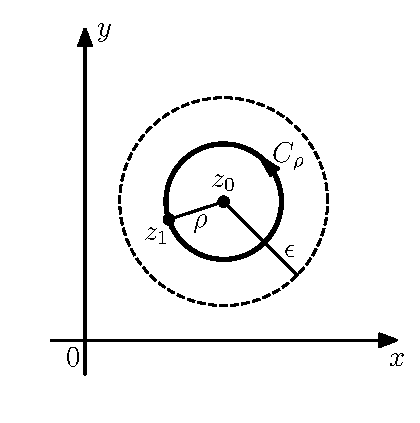
\includegraphics[width=\textwidth]{figuras/maximum_modulus_principle_lemma.pdf}
  \end{minipage}\hfill
  \begin{minipage}[c]{0.58\textwidth}
    \caption{
       Entorno \(|z-z_0|<\epsilon\) y contorno \(C_\rho\) empleados en el lema.
    }\label{fig:maximum_modulus_principle_lemma}
  \end{minipage}
\end{figure}
De la ecuación \ref{eq:gauss_mean_value_theorem}, se obtiene que 
\begin{equation}\label{eq:maximum_modulus_principle_lemma_tmp_01}
 |f(z_0)|\leq\frac{1}{2\pi}\int_0^{2\pi}|f(z_0+\rho e^{i\theta})|\,d\theta. 
\end{equation}
Por otro lado, como 
\begin{equation}\label{eq:maximum_modulus_principle_lemma_tmp_03}
 |f(z_0+\rho e^{i\theta})|\leq|f(z_0)|
 \qquad\qquad\textrm{con}\qquad\qquad
 0\leq\theta\leq2\pi, 
\end{equation}
se cumple que 
\[
 \int_0^{2\pi}|f(z_0+\rho e^{i\theta})|\,d\theta\leq\int_0^{2\pi}|f(z_0)|\,d\theta=2\pi|f(z_0)|,
\]
es decir,
\begin{equation}\label{eq:maximum_modulus_principle_lemma_tmp_02}
 |f(z_0)|\geq\frac{1}{2\pi}\int_0^{2\pi}|f(z_0+\rho e^{i\theta})|\,d\theta. 
\end{equation}
Por lo tanto, de las ecuaciones \ref{eq:maximum_modulus_principle_lemma_tmp_01} y \ref{eq:maximum_modulus_principle_lemma_tmp_02}, se obtiene que 
\[
 |f(z_0)|=\frac{1}{2\pi}\int_0^{2\pi}|f(z_0+\rho e^{i\theta})|\,d\theta,
\]
o
\[
 \int_0^{2\pi}\left[|f(z_0)|-|f(z_0+\rho e^{i\theta})|\right]\,d\theta=0.
\]
El integrando en esta integral es una función continua de \(\theta\), y por la condición \ref{eq:maximum_modulus_principle_lemma_tmp_03}, es mayor o igual a cero en el intervalo \(0\leq\theta\leq2\pi\). Como la integral es cero, el integrando debe ser cero, resultando en que
\[
 |f(z_0+\rho e^{i\theta})|=|f(z_0)|
 \qquad\qquad\textrm{con}\qquad\qquad
 0\leq\theta\leq2\pi.
\]
Esto muestra que \(|f(z)|=|f(z_0)|\) en todos los puntos \(z\) sobre el círculo \(|z-z_0|=\rho\).

Finalmente, como \(z_1\) es cualquier punto del entorno reducido \(0<|z-z_0|<\epsilon\), se observa que la ecuación \(|f(z)|=|f(z_0)|\) se satisface para todos los puntos \(z\) sobre cualquier círculo \(|z-z_0|=\rho\) con \(0<\rho<\epsilon\). En consecuencia, \(|f(z)|=|f(z_0)|\) en todos lados en el entorno \(|z-z_0|<\epsilon\). Pero del ejemplo 2 de la sección \ref{sec:analytic_functions} se sabe que cuando el módulo de una función analítica es constante en un dominio, la función en si es constante en ese dominio. Se concluye que \(f(z)=f(z_0)\) en cada punto \(z\) en el entorno, completando la prueba.

Este lema puede emplearse para probar el siguiente teorema, que se conoce como \emph{principio del módulo máximo}.

\paragraph{Teorema.} Si una función \(f\) es analítica y no constante en un dominio \(D\), entonces \(|f(z)|\) no tiene un valor máximo en \(D\). Es decir, no hay un punto \(z_0\) en el dominio tal que \(|f(z)|\leq|f(z_0)|\) para todos los puntos \(z\) en él.

Dado que \(f\) es analítica en \(D\), se probará el teorema asumiendo que \(|f(z)|\) tiene un valor máximo en algún punto \(z_0\) en \(D\) y luego mostrando que \(f(z)\) debe ser constante en \(D\). 

Sea algún punto \(P\) en \(D\) distinto de \(z_0\), y se considera una línea poligonal \(L\) perteneciente a \(D\) que se extiende desde el punto \(z_0\) hasta el punto \(P\), como se muestra en la figura \ref{fig:maximum_modulus_principle_theorem}. Además, \(d\) representa la distancia mas corta entre los puntos de \(L\) a la frontera de \(D\). Cuando \(D\) es todo el plano complejo, \(d\) puede ser cualquier número positivo. Luego se observa que hay una secuencia finita de puntos
\[
 z_0,\,z_1,\,z_2,\,\dots,\,z_{n-1},\,z_n
\]
a lo largo de \(L\) de forma tal que \(z_n\) coincide con \(P\) y
\[
 |z_k-z_{k-1}|<d
 \qquad\qquad\textrm{para}\qquad\qquad
 k=1,\,2,\,\dots,\,n.
\]
Al formar una secuencia finita de entornos
\[
 N_0,\,N_1,\,N_2,\,\dots,\,N_{n-1},\,N_n
\]
donde cada \(N_k\) tiene centro \(z_k\) y radio \(d\), se observa que \(f\) es analítica en cada uno de esos entornos, que están todos contenidos en \(D\), y que el centro de cada entorno \(N_k\) con \(k=1,\,2,\,\dots,\,n\) está contenido en el entorno \(N_{k-1}\) (ver la figura \ref{fig:maximum_modulus_principle_theorem}).
\begin{figure}[!htb]
 \begin{center}
 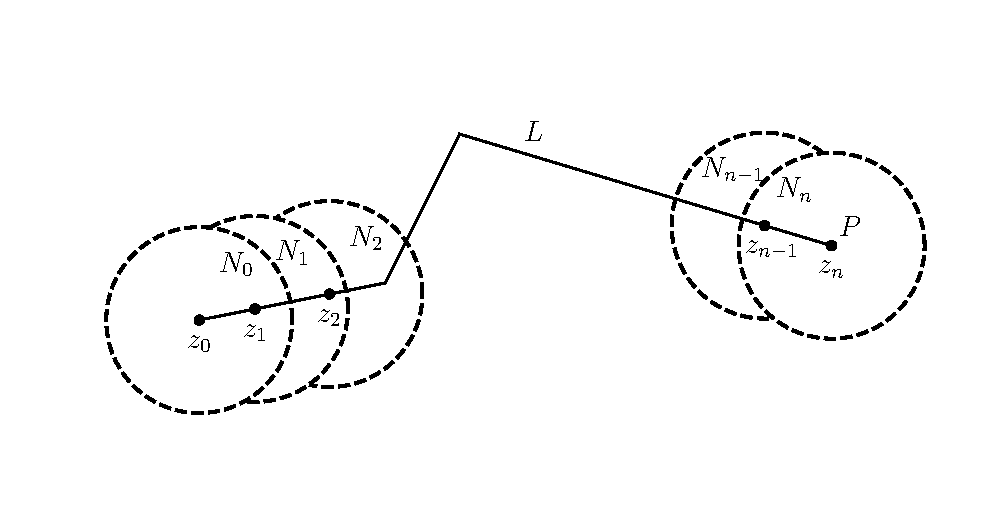
\includegraphics[width=0.8\textwidth]{figuras/maximum_modulus_principle_theorem.pdf}
 \caption{\label{fig:maximum_modulus_principle_theorem} Secuencia de entornos \(N_0,\,N_1,\,N_2,\,\dots,\,N_{n-1},\,N_n\) empleada en la demostración del principio del módulo máximo.}
 \end{center}
\end{figure}


Como se asumió que \(|f(z)|\) tiene valor máximo en \(D\) en \(z_0\), también tiene valor máximo en \(N_0\) en ese punto. Por lo tanto, de acuerdo al lema precedente, \(f(z)\) tiene valor constante \(f(z_0)\) en todo el entorno \(N_0\). En particular, \(f(z_1)=f(z_0)\). Esto significa que \(|f(z)|\leq|f(z_1)|\) para cada punto \(z\) en \(N_1\); y nuevamente puede aplicarse el lema, indicando esta vez que 
\[
 f(z)=f(z_1)=f(z_0)
\]
cuando \(z\) está en \(N_1\). Como \(z_2\) está en \(N_1\), \(f(z_2)=f(z_0)\) y por lo tanto, \(|f(z)|\leq|f(z_2)|\) cuando \(z\) está en \(N_2\); y el lema puede aplicarse nuevamente indicando que 
\[
 f(z)=f(z_2)=f(z_0)
\]
cuando \(z\) está en \(N_2\). Continuando de esta forma, eventualmente se llega al entorno \(N_n\), y se arriba al hecho de que \(f(z_n)=f(z_0)\).

Recordando que \(z_n\) coincide con el punto \(P\), que es un punto arbitrario en \(D\) distinto de \(z_0\), se concluye que \(f(z)=f(z_0)\) para cada punto \(z\) en \(D\). Como se mostró que \(f(z)\) es constante en \(D\), el teorema queda probado.

Si una función \(f\) es analítica en cada punto en el interior de una región \(R\) cerrada y acotada, también es continua en \(R\), y por lo tanto, el módulo \(|f(z)|\) tiene un valor máximo en algún punto de \(R\), como indica el teorema 4 de la sección \ref{sec:continuity_definition}. Es decir, existe una constante no negativa \(M\) tal que \(|f(z)|\leq M\) para todos los puntos \(z\) en \(R\), y la igualdad se cumple para al menos uno de esos puntos. Si \(f\) es una función constante, se cumple que \(|f(z)|=M\) para todo \(z\) en \(R\). Si \(f(z)\) no es constante, de acuerdo al teorema anterior, \(|f(z)|\neq M\) para todo punto \(z\) en el interior de \(R\). Esto conduce al siguiente importante corolario.

\paragraph{Corolario.} Supóngase que una función \(f\) es continua en una región \(R\) cerrada y acotada, y que es analítica y no constante en el interior de \(R\). Entonces, el valor máximo de \(|f(z)|\) en \(R\), que es siempre alcanzado, ocurre en la frontera de \(R\) y nunca en el interior.

Cuando la función \(f\) del corolario se expresa como \(f(z)=u(x,\,y)+iv(x,\,y)\), la función componente \(u(x,\,y)\) también tiene un valor máximo en \(R\) que es asumido en la frontera de \(R\) y nunca en el interior, donde es armónica (ver la sección \ref{sec:harmonic_functions}). Esto es porque la función compuesta \(g(z)=\exp[f(z)]\) es continua en \(R\) y analítica y no constante en el interior. Por lo tanto, por el corolario, su módulo \(|g(z)|=\exp[u(x,\,y)]\), que es continuo en \(R\), debe tomar el valor máximo en \(R\) en la frontera. Por la naturaleza creciente de la función exponencial, los valores máximos de \(\exp[u(x,\,y)]\) y \(u(x,\,y)\) se dan en el mismo punto, por lo que el valor máximo de \(u(x,\,y)\) también ocurre en la frontera.

Las propiedades de los \emph{valores mínimos} de \(|f(z)|\)  y \(u(x,\,y)\) son similares y se tratan en los ejercicios.


\subsection*{Ejercicios}

\subsubsection{Ejercicio 1}

Supóngase que \(f(z)\) es completa y que la función armónica \(u(x,\,y)=\Re[f(z)]\) tiene una cota superior \(u_0\), es decir, \(u(x,\,y)\leq u_0\) para todos los puntos \((x,\,y)\) en el plano \(xy\). Mostrar que \(u(x,\,y)\) debe ser constante en todo el plano.

\emph{Sugerencia:} aplicar el teorema de Liouville (ver la sección \ref{sec:liouville_theorem}) a la función \(g(z)=\exp[f(z)]\).

\paragraph{Solución.} Como la función \(f(z)=u(x,\,y)+iv(x,\,y)\) es completa, también lo es la función \(g(z)=\exp[f(z)]\). Además,
\[
 |g(z)|=|\exp[f(z)]|=|\exp[u(x,\,y)+iv(x,\,y)]|=|\exp[u(x,\,y)]||\exp[iv(x,\,y)]|=\exp[u(x,\,y)]\leq\exp(u_0).
\]
Como la función \(g(z)\) es completa y acotada, por el teorema de Liouville (teorema 1 de la sección \ref{sec:liouville_theorem}), \(g(z)\) es constante en todo el plano complejo. En consecuencia, \(|g(z)|=\exp[u(x,\,y)]\) es constante en todo el plano, resultando en que \(u(x,\,y)\) es constante en todo el plano por ser la función exponencial inyectiva.

\subsubsection{Ejercicio 2}

Sea \(f\) una función continua en una región \(R\) cerrada y acotada, y analítica y no constante en el interior de \(R\). Asumiendo que \(f(z)\neq0\) en todo \(R\), probar que \(|f(z)|\) tiene un valor mínimo \(m\) en \(R\) que ocurre en la frontera de \(R\) y nunca en el interior. Hacerlo aplicando el resultado correspondiente para los valores máximos de la función \(g(z)=1/f(z)\).

\paragraph{Solución.} Como \(f\) es continua en \(R\), analítica y no constante en el interior de \(R\) y \(f(z)\neq0\) en todo \(R\), la función \(g(z)=1/f(z)\) es continua en \(R\) y analítica y no constante en el interior de \(R\). Por lo tanto, \(g(z)\) cumple con las hipótesis del corolario en esta sección, y \(|g(z)|\) tiene un valor máximo que es alcanzado en algún punto de la frontera de \(R\), es decir, \(|g(z)|\leq M\) para todo \(z\) en \(R\) y la igualdad se alcanza en algún punto de la frontera. De esta forma,
\[
 |f(z)|=\frac{1}{|g(z)|}\geq\frac{1}{M}=m,
\]
y la igualdad se alcanza en algún punto de la frontera.

\subsubsection{Ejercicio 3}

Emplear la función \(f(z)=z\) para mostrar que en el ejercicio 2 la condición \(f(z)\neq0\) en todos lados en \(R\) es necesaria para obtener el resultado de dicho ejercicio. Es decir, mostrar que \(|f(z)|\) puede alcanzar su valor mínimo en un punto interior cuando el valor mínimo es cero. 

\paragraph{Solución.} Sea la región \(R\) el círculo \(|z|\leq1\) y sea la función \(f(z)=z\). De esta forma, \(R\) es cerrada y acotada y \(f\) es completa y no constante. Además, \(f(0)=0\). Por lo tanto, \(|f(0)|=0\) y \(|f(z)|=1\) en los puntos de la frontera \(|z|=1\). En este caso, \(f\) alcanza su valor mínimo en el interior de \(R\) debido a que no se cumple la condición \(f(z)\neq0\) en todo \(R\), como se requiere en las hipótesis del ejercicio 2.

\subsubsection{Ejercicio 4}

Sea \(R\) la región \(0\leq x\leq\pi,\;0\leq y\leq1\), como se muestra en la figura \ref{fig:exercise_59_04_R}. Mostrar que el módulo de la función completa \(f(z)=\sen z\) tiene el valor máximo en \(R\) en el punto \(z=\pi/2+i\) de la frontera.

\emph{Sugerencia:} escribir \(|f(z)|^2=\sen^2x+\senh^2y\) (ver la sección \ref{sec:trigonometric_functions_sin_and_cos}) y encontrar los puntos en \(R\) en donde \(\sen^2x\) y \(\senh^2y\) toman los valores mas grandes.
\begin{figure}[!htb]
  \begin{minipage}[c]{0.42\textwidth}
    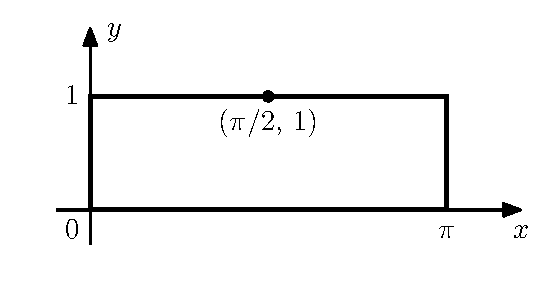
\includegraphics[width=\textwidth]{figuras/exercise_59_04_R.pdf}
  \end{minipage}\hfill
  \begin{minipage}[c]{0.48\textwidth}
    \caption{
       Frontera de la región \(R\) del ejercicio 4.
    }\label{fig:exercise_59_04_R}
  \end{minipage}
\end{figure}

\paragraph{Solución.} De la ecuación \ref{eq:sin_and_cosine_square_modulus}, el módulo al cuadrado de la función \(f(z)=\sen z\) es
\[
 |f(z)|^2=\sen^2x+\senh^2y.
\]
\begin{figure}[!htb]
  \begin{minipage}[c]{0.7\textwidth}
    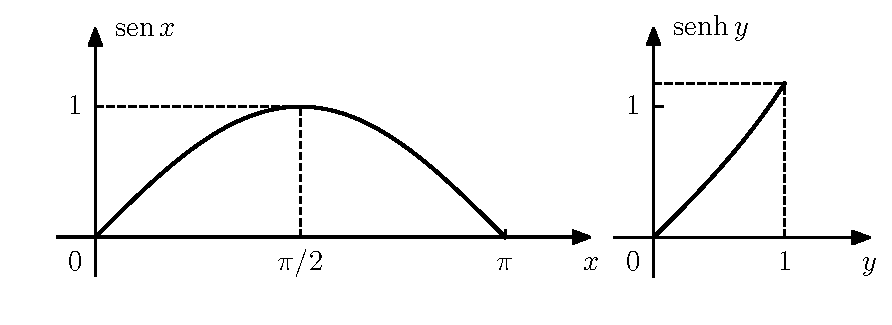
\includegraphics[width=\textwidth]{figuras/exercise_59_04_graphs.pdf}
  \end{minipage}\hfill
  \begin{minipage}[c]{0.2\textwidth}
    \caption{
       Función \(\sen x\) en el intervalo  \(0\leq x\leq\pi\) y función \(\senh y\) en el intervalo \(0\leq y\leq1\).
    }\label{fig:exercise_59_04_graphs}
  \end{minipage}
\end{figure}
Como se muestra en la figura \ref{fig:exercise_59_04_graphs}, la función \(\sen x\) tiene valor máximo en \(x=\pi/2\) cuando \(0\leq x\leq\pi\) y la función \(\senh y\) tiene valor máximo en \(y=1\) en el intervalo \(0\leq y\leq1\). Por lo tanto, el máximo de \(|f(z)|\) en \(R\) ocurre en el punto \(z=\pi/2+i\), que pertenece a la frontera de \(R\), de forma acorde a lo indicado en el corolario de esta sección. 

\subsubsection{Ejercicio 5}

Sea \(f(z)=u(x,\,y)+iv(x,\,y)\) una función que es continua en una región \(R\) cerrada y acotada, y analítica y no constante en el interior de \(R\). Probar que la función componente \(u(x,\,y)\) tiene un valor mínimo en \(R\) que ocurre en la frontera de \(R\) y nunca en el interior (ver el ejercicio 2).

\paragraph{Solución.} Al igual que \(f(z)\), la función \(g(z)=\exp[f(z)]\) es continua en una región \(R\) cerrada y acotada, y analítica y no constante en el interior de \(R\). Por lo tanto, del resultado del ejercicio 2, \(|g(z)|=\exp[u(x,\,y)]\) toma el valor mínimo en un punto de la frontera de \(R\), y como la función exponencial es monótonamente creciente, \(u(x,\,y)\) toma el valor mínimo en el mismo punto.

\subsubsection{Ejercicio 6}

Sea \(f\) la función \(f(z)=e^z\) y \(R\) la región rectangular \(0\leq x\leq 1,\;0\leq y\leq\pi\). Ilustrar los resultados de esta sección y del ejercicio 5 encontrando los puntos en \(R\) donde la función componente \(u(x,\,y)=\Re[f(z)]\) alcanza los valores máximo y mínimo.

\paragraph{Solución.} Como
\[
 f(z)=e^z=e^xe^{iy}=e^x(\cos y+i\sen y),
\]
se tiene que 
\[
 u(x,\,y)=e^x\cos y.
\]
De las gráficas de las funciones \(e^x\) y \(\cos y\) que se muestran en la figura \ref{fig:exercise_59_06_graphs} se deduce que el valor máximo de \(u(x,\,y)\) en \(R\) ocurre cuando \(x=1\) y \(y=0\), es decir, en \(z=1\), y en ese caso, \(u(x,\,y)=e\). Además, el valor mínimo ocurre en \(x=1\) y \(y=\pi\), es decir, en \(z=1+\pi i\), y en ese caso, \(u(x,\,y)=-e\). Se observa que los valores máximo y mínimo ocurren en la frontera de \(R\).
\begin{figure}[!htb]
  \begin{minipage}[c]{0.7\textwidth}
    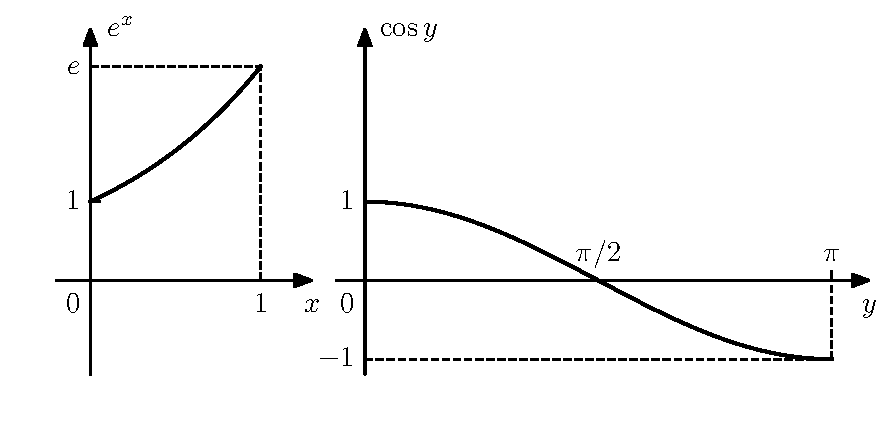
\includegraphics[width=\textwidth]{figuras/exercise_59_06_graphs.pdf}
  \end{minipage}\hfill
  \begin{minipage}[c]{0.2\textwidth}
    \caption{
       Función \(e^x\) en el intervalo  \(0\leq x\leq1\) y función \(\cos y\) en el intervalo \(0\leq y\leq\pi\).
    }\label{fig:exercise_59_06_graphs}
  \end{minipage}
\end{figure}

\subsubsection{Ejercicio 7}

Sea la función \(f(z)=u(x,\,y)+iv(x,\,y)\) continua en una región \(R\) cerrada y acotada, y analítica y no constante en el interior de \(R\). Mostrar que la función componente \(v(x,\,y)\) tiene valores máximos y mínimos en \(R\) que son alcanzados en la frontera de \(R\) y nunca en el interior, donde es armónica.

\emph{Sugerencia:} aplicar los resultados de esta sección y del ejercicio 5 a la función \(g(z)=-if(z)\). 

\paragraph{Solución.} Sea la función \(g(z)=-if(z)\). Al igual que \(f(z)\), \(g(z)\) es continua en la región \(R\) cerrada y acotada, y analítica y no constante en el interior de \(R\). Además, como
\[
 g(z)=-if(z)=v(x,\,y)-iu(x,\,y),
\]
el componente real de \(g(z)\) es \(v(x,\,y)\), y de los resultados de esta sección y del ejercicio 5, \(v(x,\,y)\) tiene valores máximos y mínimos en \(R\) que son alcanzados en la frontera de \(R\) y nunca en el interior.

\subsubsection{Ejercicio 8}

Sea \(z_0\) un cero del polinomio
\[
 P(z)=a_0+a_1z+a_2z^2+\dots+a_nz^n,
 \qquad\qquad
 a_n\neq0,
\]
de grado \(n\), con \(n\geq1\). Mostrar de la forma siguiente que 
\[
 P(z)=(z-z_0)Q(z)
\]
donde \(Q(z)\) es un polinomio de grado \(n-1\).
\begin{enumerate}
 \item[(\textit{a})] Verificar que 
 \[
  z^k-z_0^k=(z-z_0)(z^{k-1}+z^{k-2}z_0+\dots+zz_0^{k-2}+z_0^{k-1}),
  \qquad\qquad\textrm{con}\qquad\qquad
  k=2,\,3,\,\dots.
 \]
 \item[(\textit{b})] Emplear la factorización de la parte (\textit{a}) para mostrar que 
 \[
  P(z)-P(z_0)=(z-z_0)Q(z)
 \]
 donde \(Q(z)\) es un polinomio de grado \(n-1\), y deducir el resultado deseado a partir de esto.
\end{enumerate}

\paragraph{Solución.} 
\begin{enumerate}
 \item[(\textit{a})] Desarrollando el lado derecho de la igualdad que se quiere verificar, se ve que 
 \begin{align*}
  (z-z_0)(z^{k-1}+z^{k-2}z_0+\dots+zz_0^{k-2}+z_0^{k-1})&=(z^k+z^{k-1}z_0+\dots+z^2z_0^{k-2}+zz_0^{k-1})\\
   &\qquad-(z^{k-1}z_0+z^{k-2}z_0^2+\dots+zz_0^{k-1}+z_0^k)\\
   &=z^k-z_0^k.
 \end{align*}
 \item[(\textit{b})] Se observa que 
 \begin{align*}
  P(z)-P(z_0)&=(a_0+a_1z+a_2z^2+\dots+a_nz^n)-(a_0+a_1z_0+a_2z_0^2+\dots+a_nz_0^n)\\
   &\overset{(1)}{=}a_1(z-z_0)+a_2(z-z_0)(z+z_0)+\dots\\
   &\qquad+a_n(z-z_0)(z^{n-1}+z^{n-2}z_0+\dots+zz_0^{n-2}+z_0^{n-1})\\
   &=(z-z_0)\left[a_1+a_2(z-z_0)+\dots+a_n(z^{n-1}+z^{n-2}z_0+\dots+zz_0^{n-2}+z_0^{n-1})\right]\\
   &=(z-z_0)Q(z),
 \end{align*}
donde 
\[
 Q(z)=a_1+a_2(z-z_0)+\dots+a_n(z^{n-1}+z^{n-2}z_0+\dots+zz_0^{n-2}+z_0^{n-1})
\]
es un polinomio de grado \(n-1\), y en \((1)\) se empleó el resultado de la parte (\textit{a}). Finalmente, como \(z_0\) es un cero de \(P(z)\), se cumple que \(P(z_0)=0\) resultando en que 
\[
 P(z)=(z-z_0)Q(z).
\]
\end{enumerate}

\chapter{Series}

Este capítulo es dedicado a la representación de funciones analíticas en series. Se presentan los teoremas que garantizan la existencia de dichas representaciones y se proveen herramientas para la manipulación de series.

\section{Convergencia de secuencias}\label{sec:convergence_of_sequences}

Una \emph{secuencia infinita} \(z_1,\,z_2,\,\dots,\,z_n,\,\dots\) de números complejos tiene un límite \(z\) si para cada número positivo \(\epsilon\) existe un número entero positivo \(n_0\) tal que 
\begin{equation}\label{eq:sequences_convergence_definition}
 |z_n-z|<\epsilon
 \qquad\qquad 
 \textrm{cuando}
 \qquad\qquad
 n>n_0. 
\end{equation}
Geométricamente esto significa que para valores de \(n\) suficientemente grandes, los puntos \(z_n\) están en un entorno \(\epsilon\) dado de \(z\). El hecho de que \(\epsilon\) puede elegirse tan pequeño como se desee implica que los puntos \(z_n\) se acercan arbitrariamente a \(z\) a medida que el subíndice crece. Observar que el valor de \(n_0\) depende en general de \(\epsilon\).

Una secuencia puede tener a los sumo un límite, es decir, un límite \(z\) es único si existe, como se muestra en el ejercicio 5 de la sección \ref{sec:convergence_of_series}. Cuando el límite \(z\) existe se dice que la secuencia \emph{converge} a \(z\) y se denota
\[
 \lim_{n\to\infty}z_n=z.
\]
Si la secuencia no tiene límite se dice que \emph{diverge}.

\paragraph{Teorema.} Supóngase que \(z_n=x_n+iy_n\), con \(n=1,\,2,\,\dots\), y \(z=x+iy\). Entonces
\begin{equation}\label{eq:sequences_convergence_re_im_thoerm_direct}
 \lim_{n\to\infty}z_n=z 
\end{equation}
si y solo si
\begin{equation}\label{eq:sequences_convergence_re_im_thoerm_reciprocal}
 \lim_{n\to\infty}x_n=x
 \qquad\qquad\textrm{y}\qquad\qquad
 \lim_{n\to\infty}y_n=y. 
\end{equation}

Para probar el teorema se asume primero que se cumplen las condiciones \ref{eq:sequences_convergence_re_im_thoerm_reciprocal} y se obtendrá la condición \ref{eq:sequences_convergence_re_im_thoerm_direct} a partir de ellas. De acuerdo a las condiciones \ref{eq:sequences_convergence_re_im_thoerm_reciprocal}, para cada número positivo \(\epsilon\), existen los enteros \(n_1\) y \(n_2\) tal que  
\[
 |x_n-x|<\frac{\epsilon}{2}
 \qquad\qquad 
 \textrm{cuando}
 \qquad\qquad
 n>n_1
\]
y
\[
 |y_n-y|<\frac{\epsilon}{2}
 \qquad\qquad 
 \textrm{cuando}
 \qquad\qquad
 n>n_2.
\]
Por lo tanto, si \(n_0\) es el mayor de los dos enteros \(n_1\) y \(n_2\),
\[
 |x_n-x|<\frac{\epsilon}{2}
 \qquad\textrm{y}\qquad
 |y_n-y|<\frac{\epsilon}{2}
 \qquad\qquad\textrm{cuando}\qquad\qquad
 n>n_0.
\]
Como
\[
 |z_n-z|=|(x_n+iy_n)-(x+iy)|=|(x_n-x)+i(y_n-y)|\leq|x_n-x|+|y_n-y|,
\]
se cumple que 
\[
 |z_n-z|<\frac{\epsilon}{2}+\frac{\epsilon}{2}=\epsilon
 \qquad\qquad\textrm{cuando}\qquad\qquad
 n>n_0,
\]
que es lo que se quería probar. 

Recíprocamente, si se comienza con la condición \ref{eq:sequences_convergence_re_im_thoerm_direct}, se sabe que para todo número positivo \(\epsilon\), existe un entero positivo \(n_0\) tal que 
\[
 |z_n-z|<\epsilon
 \qquad\qquad\textrm{cuando}\qquad\qquad
 n>n_0.
\]
Pero
\[
|x_n-x|\leq|(x_n-x)+i(y_n-y)|=|(x_n+iy_n)-(x+iy)|=|z_n-z| 
\]
y
\[
|y_n-y|\leq|(x_n-x)+i(y_n-y)|=|(x_n+iy_n)-(x+iy)|=|z_n-z|
\]
y esto significa que 
\[
 |x_n-x|<\epsilon
 \qquad\qquad\textrm{y}\qquad\qquad
 |y_n-y|<\epsilon
 \qquad\qquad\textrm{cuando}\qquad\qquad
 n>n_0,
\]
que es la condición \ref{eq:sequences_convergence_re_im_thoerm_reciprocal}.

Observar que el teorema permite escribir 
\[
 \lim_{n\to\infty}(x_n+iy_n)=\lim_{n\to\infty}x_n+i\lim_{n\to\infty}y_n
\]
cuando se sabe que los dos límites de la derecha existen o el límite de la izquierda existe.

\paragraph{Ejemplo 1.} La secuencia
\[
 z_n=-1+i\frac{(-1)^n}{n^2},
 \qquad\qquad
 n=1,\,2,\,\dots.
\]
converge a \(-1\) ya que 
\[
 \lim_{n\to\infty}\left[-1+i\frac{(-1)^n}{n^2}\right]=\lim_{n\to\infty}(-1)+i\lim_{n\to\infty}\frac{(-1)^n}{n^2}=-1+i0=-1.
\]

El siguiente ejemplo muestra que hay que tener cuidado al adaptar el teorema a coordenadas polares.

\paragraph{Ejemplo 2.} Considérese la misma secuencia
\[
 z_n=-1+i\frac{(-1)^n}{n^2},
 \qquad\qquad
 n=1,\,2,\,\dots
\]
del ejemplo 1. Si se emplean las coordenadas polares
\[
 r_n=|z_n|
 \qquad\qquad\textrm{y}\qquad\qquad
 \Theta_n=\Arg z_n,
 \qquad\qquad
 n=1,\,2,\,\dots,
\]
donde \(\Arg z_n\) denota el argumento principal (\(-\pi<\Theta_n\leq\pi\)), se observa que por un lado,
\[
 \lim_{n\to\infty}r_n=\lim_{n\to\infty}\sqrt{1+\frac{1}{n^4}}=1.
\]
Pero considerando que \(z_n\) pertenece al segundo cuadrante si \(n\) es par y al tercer cuadrante si \(n\) es impar, se tiene que 
\[
 \lim_{n\to\infty}\Theta_{2n}=\pi
 \qquad\qquad\textrm{y}\qquad\qquad
 \lim_{n\to\infty}\Theta_{2n-1}=-\pi,
 \qquad\qquad
 n=1,\,2,\,\dots,
\]
lo que indica que el límite de \(\Theta_n\) no existe cuando \(n\) tiende a infinito. Ver además el ejercicio 2 de la sección \ref{sec:convergence_of_series}.

\section{Convergencia de series}\label{sec:convergence_of_series}

Una \emph{serie} infinita
\begin{equation}\label{eq:series_convergence_series_definition}
 \sum_{n=1}^\infty z_n=z_1+z_2+\dots+z_n+\dots 
\end{equation}
de números complejos \emph{converge} a la \emph{suma} \(S\) si la secuencia 
\begin{equation}\label{eq:series_convergence_partial_sums}
 S_N=\sum_{n=1}^N z_n=z_1+z_2+\dots+z_N,
 \qquad\qquad
 N=1,\,2,\,\dots, 
\end{equation}
de \emph{sumas parciales} converge a \(S\). En ese caso, se escribe
\[
 \sum_{n=1}^\infty z_n=S.
\]
Notar que como una secuencia puede tener a lo sumo un límite, una serie puede tener a los sumo una suma. Cuando una serie no converge se dice que \emph{diverge}.

\paragraph{Teorema.} Supóngase que \(z_n=x_n+iy_n\), con \(n=1,\,2,\,\dots\), y \(S=X+iY\). Entonces
\begin{equation}\label{eq:series_convergence_re_im_thoerm_direct}
 \sum_{n=1}^\infty z_n=S
\end{equation}
si y solo si
\begin{equation}\label{eq:series_convergence_re_im_thoerm_reciprocal}
 \sum_{n=1}^\infty x_n=X
 \qquad\qquad\textrm{y}\qquad\qquad
 \sum_{n=1}^\infty y_n=Y. 
\end{equation}

Este teorema indica que 
\[
 \sum_{n=1}^\infty(x_n+iy_n)=\sum_{n=1}^\infty x_n+i\sum_{n=1}^\infty y_n
\]
si se sabe que las dos series de la derecha convergen o la serie de la izquierda lo hace.

Para probar el teorema, se escriben las sumas parciales \ref{eq:series_convergence_partial_sums} como
\begin{equation}\label{eq:partial_sum_tmp}
 S_N=X_N+iY_N 
\end{equation}
donde
\[
 X_N=\sum_{n=1}^Nx_n
 \qquad\qquad\textrm{y}\qquad\qquad
 Y_N=\sum_{n=1}^Ny_n.
\]
La afirmación \ref{eq:series_convergence_re_im_thoerm_direct} es verdadera si y solo si
\begin{equation}\label{eq:partial_sum_limit_tmp}
 \lim_{N\to\infty}S_N=S, 
\end{equation}
y considerando la relación de la ecuación \ref{eq:partial_sum_tmp}, del teorema de secuencias de la sección \ref{sec:convergence_of_sequences}, el límite \ref{eq:partial_sum_limit_tmp} se cumple si y solo si
\begin{equation}\label{eq:tmp_partial_sum_limit_re_img}
 \lim_{N\to\infty}X_N=X
 \qquad\qquad\textrm{y}\qquad\qquad
 \lim_{N\to\infty}Y_N=Y. 
\end{equation}
Se concluye que los límites \ref{eq:tmp_partial_sum_limit_re_img} implican la afirmación \ref{eq:series_convergence_re_im_thoerm_direct} y recíprocamente. Como \(X_N\) y \(Y_N\) son las sumas parciales de \ref{eq:series_convergence_re_im_thoerm_reciprocal}, en teorema queda demostrado.

El teorema es útil para mostrar que algunas de las propiedades familiares de series de números reales en cálculo se trasladan a series cuyos términos son números complejos. Para ilustrar como se hace, a continuación se incluyen dos propiedades y se presentan como corolarios.

\paragraph{Corolario 1.} Si una serie de números complejos converge, el término \(n\)-ésimo converge a cero cuando \(n\) tiende a infinito.

Asumiendo que la serie \ref{eq:series_convergence_series_definition} converge, del teorema se sabe que si
\[
 z_n=x_n+iy_n,
 \qquad\qquad
 n=1,\,2,\,\dots, 
\]
cada una de las series
\[
 \sum_{n=1}^\infty x_n
 \qquad\qquad\textrm{y}\qquad\qquad
 \sum_{n=1}^\infty y_n 
\]
converge. Además, se sabe de cálculo que el término \(n\)-ésimo de una serie convergente de números reales tiende a cero cuando \(n\) tiende a infinito (ver por ejemplo la sección 11.2 de \cite{stewart2016essential}) y por lo tanto
\[
 \lim_{n\to\infty}x_n=0
 \qquad\qquad\textrm{y}\qquad\qquad
 \lim_{n\to\infty}y_n=0,
\]
y por el teorema de la sección \ref{sec:convergence_of_sequences},
\[
 \lim_{n\to\infty}z_n=\lim_{n\to\infty}x_n+i\lim_{n\to\infty}y_n=0+i0=0,
\]
concluyendo la prueba del corolario 1.

De este corolario surge que los términos de una serie convergente son \emph{acotados}, es decir, cuando la serie \ref{eq:series_convergence_series_definition} converge, existe una constante positiva \(M\) tal que \(|z_n|\leq M\) para cada \(n\), como se muestra en el ejercicio 9 de esta sección.

Otra importante propiedad de las series de números complejos que se traslada de la propiedad correspondiente las series de números reales, es la de \emph{convergencia absoluta} (ver la sección 11.6 de \cite{stewart2016essential}, por ejemplo). La serie \ref{eq:series_convergence_series_definition} se dice que \emph{converge absolutamente} si la serie
\[
 \sum_{n=1}^\infty|z_n|=\sum_{n=1}^\infty\sqrt{x_n^2+y_n^2},
\]
de números reales \(\sqrt{x_n^2+y_n^2}\) converge, donde \(z_n=x_n+iy_n.\)

\paragraph{Corolario 2.} La convergencia absoluta de una serie de números complejos implica la convergencia de la serie.

Para probar este corolario, se asume que la serie \ref{eq:series_convergence_series_definition} converge absolutamente. Como
\[
 |x_n|\leq\sqrt{x_n^2+y_n^2}
 \qquad\qquad\textrm{y}\qquad\qquad
 |y_n|\leq\sqrt{x_n^2+y_n^2},
\]
se sabe por las pruebas de comparación en cálculo (ver la sección 11.4 de \cite{stewart2016essential}, por ejemplo) que las series 
\[
 \sum_{n=1}^\infty|x_n|
 \qquad\qquad\textrm{y}\qquad\qquad
 \sum_{n=1}^\infty|y_n|
\]
convergen. Además, como la convergencia absoluta de una serie de números reales implica la convergencia de la serie (ver la sección 11.6 de \cite{stewart2016essential}, por ejemplo), cada una de las series
\[
 \sum_{n=1}^\infty x_n
 \qquad\qquad\textrm{y}\qquad\qquad
 \sum_{n=1}^\infty y_n 
\]
converge, y por el teorema de esta sección, la serie \ref{eq:series_convergence_series_definition} converge, concluyendo la prueba del corolario 2.

Al establecer el hecho de que la suma de una serie es un número \(S\) dado, es conveniente en ocasiones definir el \emph{resto} \(\rho_N\) producido por \(N\) términos de la suma parcial \ref{eq:series_convergence_partial_sums}:
\[
 \rho_N=S-S_N.
\]
Se observa que una serie converge a un número \(S\) si y solo si la secuencia de restos tiende a cero. Se hará un uso considerable de esta observación en el tratamiento de \emph{series de potencias}. Éstas son series de la forma
\[
 \sum_{n=0}^\infty a_n(z-z_0)^n=a_0+a_1(z-z_0)+a_2(z-z_0)^2+\dots+a_n(z-z_0)^n+\dots,
\]
donde \(z_0\) y los coeficientes \(a_n\) son constantes complejas y \(z\) puede ser cualquier punto de una región determinada que contiene a \(z_0\). En dichas series, que involucran a una variable \(z\), se denotarán a las sumas, a las sumas parciales y a los restos como \(S(z)\), \(S_N(z)\) y \(\rho_N(z)\) respectivamente.

\paragraph{Ejemplo.} Con la ayuda de restos es fácil verificar que
\begin{equation}\label{eq:geometric_series}
 \sum_{n=0}^\infty z^n=\frac{1}{1-z}
 \qquad\qquad\textrm{cuando}\qquad\qquad
 |z|<1.
\end{equation}
Para hacerlo, se parte considerando la identidad
\begin{equation}\label{eq:geometric_series_to_N-1}
 1+z+z^2+\dots+z^{N-1}=\frac{1-z^N}{1-z}
 \qquad\qquad\textrm{cuando}\qquad\qquad
 z\neq 1. 
\end{equation}
Esta identidad puede comprobarse denominando 
\[
 S_N(z)=1+z+z^2+\dots+z^{N-1}
\]
y observando que 
\[
 S_N(z)-zS_N(z)=1-z^N
 \qquad\Leftrightarrow\qquad
 (1-z)S_N(z)=1-z^N
 \qquad\Leftrightarrow\qquad
 S_N(z)=\frac{1-z^N}{1-z},
\]
resultando en la ecuación \ref{eq:geometric_series_to_N-1}. Si
\[
 S(z)=\frac{1}{1-z},
\]
se tiene que 
\[
 \rho_N(z)=S(z)-S_N(z)=\frac{1}{1-z}-\frac{1-z^N}{1-z}=\frac{z^N}{1-z}
 \qquad\textrm{cuando}\qquad
 z\neq 1.
\]
Por lo tanto
\[
 |\rho_N(z)|=\frac{|z|^N}{|1-z|},
\]
resultando claro que el resto \(\rho_N(z)\) tiende a cero cuando \(|z|<1\) pero no si \(|z|\geq1\), estableciendo la ecuación \ref{eq:geometric_series}.

\subsection*{Ejercicios}

\subsubsection{Ejercicio 1}

Emplear la definición \ref{eq:sequences_convergence_definition} de la existencia del límite de una secuencia para mostrar que 
\[
 \lim_{n\to\infty}\left(\frac{1}{n^2}+i\right)=i.
\]

\paragraph{Solución.} De la definición \ref{eq:sequences_convergence_definition} con 
\[
 z_n=\frac{1}{n^2}+i
 \qquad\qquad\textrm{y}\qquad\qquad
 z=i,
\]
para cada número positivo \(\epsilon\)
\[
 \left|\frac{1}{n^2}+i-i\right|<\epsilon
 \qquad\qquad\Leftrightarrow\qquad\qquad 
 \frac{1}{n^2}<\epsilon
 \qquad\qquad\Leftrightarrow\qquad\qquad 
 n>\frac{1}{\sqrt{\epsilon}}.
\]
Por lo tanto, eligiendo a \(n_0\) como el entero inmediatamente superior a \(1/\sqrt{\epsilon}\), la condición \ref{eq:sequences_convergence_definition} se cumple para todo \(n>n_0\).

\subsubsection{Ejercicio 2}

Sea \(\Theta_n\) con \(n=1,\,2,\,\dots\) el argumento principal de los números 
\[
 z_n=1+i\frac{(-1)^n}{n^2}
 \qquad\qquad\textrm{con}\qquad\qquad
 n=1,\,2,\,\dots,
\]
indicar porque 
\[
 \lim_{n\to\infty}\Theta_n=0.
\]
Comparar con el resultado del ejemplo 2 de la sección \ref{sec:convergence_of_sequences}. 

\paragraph{Solución.} Considerando que los números \(z_n\) pertenecen al primer cuadrante cuando \(n\) es par y al cuarto cuadrante cuando \(n\) es impar y observando que la parte imaginaria tiende a cero cuando \(n\) tiende a infinito  se tiene que 
\[
 \lim_{n\to\infty}\Theta_{2n}=0^+
 \qquad\qquad\textrm{y}\qquad\qquad
 \lim_{n\to\infty}\Theta_{2n-1}=0^-,
 \qquad\qquad
 n=1,\,2,\,\dots,
\]
concluyendo que 
\[
 \lim_{n\to\infty}\Theta_n=0.
\]

\subsubsection{Ejercicio 3}

Emplear la desigualdad \(||z_n|-|z||\leq|z_n-z|\) (ver la sección \ref{sec:triangle_inequality} para mostrar que 
\[
 \textrm{si}\qquad
 \lim_{n\to\infty}z_n=z
 \qquad\textrm{entonces}\qquad
 \lim_{n\to\infty}|z_n|=|z|.
\]

\paragraph{Solución.} Como 
\[
 \lim_{n\to\infty}z_n=z,
\]
por definición de límite, para cualquier número positivo \(\epsilon\), existe un entero positivo \(n_0\) tal que \(|z_n-z|<\epsilon\) para todo \(n>n_0\). Pero como
\[
 ||z_n|-|z||\leq|z_n-z|
\]
también se cumple que \(||z_n|-|z||<\epsilon\) para todo \(n>n_0\) y por lo tanto,
\[
 \lim_{n\to\infty}|z_n|=|z|.
\]

\subsubsection{Ejercicio 4}

Escribir \(z=re^{i\theta}\), donde \(0<r<1\), en la identidad \ref{eq:geometric_series}. Luego, con la ayuda del teorema de la sección \ref{sec:convergence_of_series}, mostrar que 
\[
 \sum_{n=1}^\infty r^n\cos n\theta=\frac{r\cos\theta-r^2}{1-2r\cos\theta+r^2}
 \qquad\qquad\textrm{y}\qquad\qquad
 \sum_{n=1}^\infty r^n\sen n\theta=\frac{r\sen \theta}{1-2r\cos\theta+r^2}
\]
cuando \(0<r<1\). Observar que esas fórmulas también son válidas cuando \(r=0\).

\paragraph{Solución.} Multiplicando ambos lados de la igualdad \ref{eq:geometric_series} por \(z\) se obtiene la identidad 
\[
 \sum_{n=0}^\infty z^{n+1}=\frac{z}{1-z}
 \qquad\qquad\textrm{cuando}\qquad\qquad
 |z|<1,
\]
y sustituyendo \(n+1\) por \(n\) resulta en
\begin{equation}\label{eq:geometric_series_alt}
 \sum_{n=1}^\infty z^n=\frac{z}{1-z}
 \qquad\qquad\textrm{cuando}\qquad\qquad
 |z|<1. 
\end{equation}
Sustituyendo \(z=re^{i\theta}\), el lado izquierdo de la igualdad \ref{eq:geometric_series_alt} es
\[
 \sum_{n=1}^\infty\left(re^{i\theta}\right)^n=\sum_{n=1}^\infty r^ne^{in\theta}=\sum_{n=1}^\infty r^n(\cos n\theta+i\sen n\theta)=\sum_{n=1}^\infty\left(r^n\cos n\theta+ir^n\sen n\theta\right),
\]
y el lado izquierdo de la igualdad \ref{eq:geometric_series_alt} queda 
\[
 \frac{re^{i\theta}}{1-re^{i\theta}}=\frac{re^{i\theta}(1-re^{-i\theta})}{(1-re^{i\theta})(1-re^{-i\theta})}
 =\frac{re^{i\theta}-r^2}{1-re^{-i\theta}-re^{i\theta}+r^2}
 =\frac{r(\cos\theta+i\sen\theta)-r^2}{1-2r\cos\theta+r^2}.
\]
Combinando los resultados, se obtiene que 
\[
 \sum_{n=1}^\infty\left(r^n\cos n\theta+ir^n\sen n\theta\right)=\frac{r\cos\theta-r^2+ir\sen\theta}{1-2r\cos\theta+r^2},
\]
y por el teorema de la sección \ref{sec:convergence_of_series}, se concluye que 
\[
 \sum_{n=1}^\infty r^n\cos n\theta=\frac{r\cos\theta-r^2}{1-2r\cos\theta+r^2}
 \qquad\qquad\textrm{y}\qquad\qquad
 \sum_{n=1}^\infty r^n\sen n\theta=\frac{r\sen \theta}{1-2r\cos\theta+r^2}.
\]

\subsubsection{Ejercicio 5}

Mostrar que el límite de una secuencia convergente de números complejos es único apelando al resultado correspondiente de secuencias de números reales.

\paragraph{Solución.} Del teorema de la sección \ref{sec:convergence_of_sequences}, en una secuencia de números complejos convergente \(z_n=x_n+iy_n\) se cumple que 
\[
 \lim_{n\to\infty}z_n=\lim_{n\to\infty}(x_n+iy_n)=\lim_{n\to\infty}x_n+i\lim_{n\to\infty}y_n.
\]
Como \(x_n\) y \(y_n\) son secuencias de números reales, su límite es único (ver por ejemplo, la sección 7 de \cite{kenneth2013elementary}), concluyendo que el límite de la secuencia \(z_n\) de números complejos también es único.

\subsubsection{Ejercicio 6}

Mostrar que 
\[
 \textrm{si}\qquad 
 \sum_{n=1}^\infty z_n=S
 \qquad\qquad\textrm{entonces}\qquad\qquad
 \sum_{n=1}^\infty\overline{z_n}=\overline{S}.
\]

\paragraph{Solución.} Con \(z_n=x_n+iy_n\) y \(S=X+iY\), del teorema de esta sección, 
\[
 \sum_{n=1}^\infty z_n=S
 \qquad\qquad\Leftrightarrow\qquad\qquad
 \sum_{n=1}^\infty x_n=X
 \qquad\qquad\textrm{y}\qquad\qquad
 \sum_{n=1}^\infty y_n=Y. 
\]
Por lo tanto,
\[
 \sum_{n=1}^\infty\overline{z_n}=\sum_{n=1}^\infty(x_n-iy_n)=\sum_{n=1}^\infty[x_n+i(-y_n)]\overset{(a)}{=}\sum_{n=1}^\infty x_n+i\sum_{n=1}^\infty(-y_n)\overset{(b)}{=}X-iY=\overline{S},
\]
donde en \((a)\) se tuvo en cuenta que las series reales
\[
 \sum_{n=1}^\infty x_n
 \qquad\qquad\textrm{y}\qquad\qquad
 \sum_{n=1}^\infty y_n
\]
convergen y por lo tanto también converge la serie 
\[
 \sum_{n=1}^\infty(-y_n),
\]
y en \((b)\) que
\[
\textrm{como}\qquad\qquad
 \sum_{n=1}^\infty y_n=Y
 \qquad\qquad\textrm{entonces}\qquad\qquad
 \sum_{n=1}^\infty(-y_n)=-Y.
\]

\subsubsection{Ejercicio 7}

Si \(c\) es cualquier número complejo, mostrar que 
\[
 \textrm{si}\qquad 
 \sum_{n=1}^\infty z_n=S
 \qquad\qquad\textrm{entonces}\qquad\qquad
 \sum_{n=1}^\infty cz_n=cS.
\]

\paragraph{Solución.} Con \(z_n=x_n+iy_n\) y \(S=X+iY\), del teorema de esta sección, 
\[
 \sum_{n=1}^\infty z_n=S
 \qquad\qquad\Leftrightarrow\qquad\qquad
 \sum_{n=1}^\infty x_n=X
 \qquad\qquad\textrm{y}\qquad\qquad
 \sum_{n=1}^\infty y_n=Y. 
\]
Por lo tanto,
\[
 \sum_{n=1}^\infty cz_n=\sum_{n=1}^\infty c(x_n-iy_n)=\sum_{n=1}^\infty[cx_n+i(cy_n)]=\sum_{n=1}^\infty cx_n+i\sum_{n=1}^\infty cy_n=cX+icY=c(X+iY),
\]
donde se tuvo en cuenta que como
\[
 \sum_{n=1}^\infty x_n=X
 \qquad\textrm{y}\qquad
 \sum_{n=1}^\infty y_n=Y.
\]
se cumple que 
\[
 \sum_{n=1}^\infty cx_n=cX
 \qquad\textrm{y}\qquad
 \sum_{n=1}^\infty cy_n=cY.
\]

\subsubsection{Ejercicio 8}

Recurriendo a los resultados correspondientes de series de números reales y al teorema en esta sección mostrar que 
\[
 \textrm{si}\qquad 
 \sum_{n=1}^\infty z_n=S
 \qquad\textrm{y}\qquad
 \sum_{n=1}^\infty w_n=T
 \qquad\qquad\textrm{entonces}\qquad\qquad
 \sum_{n=1}^\infty(z_n+w_n)=S+T.
\]

\paragraph{Solución.} Con \(z_n=x_n+iy_n\), \(w_n=u_n+iv_n\), \(S=X+iY\) y \(T=U+iV\), del teorema de esta sección, 
\[
 \sum_{n=1}^\infty z_n=S
 \qquad\qquad\Leftrightarrow\qquad\qquad
 \sum_{n=1}^\infty x_n=X
 \qquad\qquad\textrm{y}\qquad\qquad
 \sum_{n=1}^\infty y_n=Y
\]
y
\[
 \sum_{n=1}^\infty w_n=T
 \qquad\qquad\Leftrightarrow\qquad\qquad
 \sum_{n=1}^\infty u_n=U
 \qquad\qquad\textrm{y}\qquad\qquad
 \sum_{n=1}^\infty v_n=V.
\]
Por lo tanto,
\begin{align*}
 \sum_{n=1}^\infty(z_n+w_n)&=\sum_{n=1}^\infty[(x_n+iy_n)+(u_n+iv_n)]\\
  &=\sum_{n=1}^\infty[(x_n+u_n)+i(y_n+v_n)]\\ 
  &=\sum_{n=1}^\infty(x_n+u_n)+i\sum_{n=1}^\infty(y_n+v_n)\\ 
  &=(X+U)+i(Y+V)\\
  &=(X+iY)+(U+iV)\\
  &=S+T.
\end{align*}

\subsubsection{Ejercicio 9}

Asúmase que la secuencia \(z_n\) con \(n=1,\,2,\,\dots\) converge al número \(z\). Mostrar que existe un número positivo \(M\) tal que la desigualdad \(|z_n|\leq M\) se cumple para todo \(n\). Hacerlo de las siguientes formas:
\begin{enumerate}
 \item[(\textit{a})] Notar que hay un entero positivo \(n_0\) tal que 
 \[
  |z_n|=|z+(z_n-z)|<|z|-1
 \]
 para todo \(n>n_0\).
 \item[(\textit{b})] Escribir \(z_n=x_n+iy_n\) y recordar de la teoría de secuencias de números reales que la convergencia de \(x_n\) y \(y_n\) con \(n=1,\,2,\,\dots\), implica que \(|x_n|\leq M_1\) y \(|y_n|\leq M_2\) para \(n=1,\,2,\,\dots\) para algún par de números positivos \(M_1\) y \(M_2\).
\end{enumerate}

\paragraph{Solución.} 
\begin{enumerate}
 \item[(\textit{a})] Se observa que 
 \[
  |z_n|=|z+(z_n-z)|\overset{(a)}{\leq}|z|+|z_n-z|\overset{(b)}{<}|z|+1
 \]
 para todo \(n>n_0\), donde en \((a)\) se empleó la desigualdad triangular y en \((b)\) se empleó la definición \ref{eq:sequences_convergence_definition} del límite de una secuencia con \(\epsilon=1\), es decir, que existe un número entero positivo tal que 
 \[
  |z_n-z|<1
 \qquad\qquad 
 \textrm{cuando}
 \qquad\qquad
 n>n_0. 
 \]
 Definiendo 
 \[
  M=\max\{|z_0|,\,|z_1|,\,\dots,\,|z_{n_0}|,\,|z|+1\}
 \]
 se concluye que 
 \[
  |z_n|\leq M
 \]
 para \(n=1,\,2,\,\dots\).
 \item[(\textit{b})] Con \(z_n=x_n+iy_n\) y \(z=x+iy\), como \(z_n\) converge a \(z\), del teorema de la sección \ref{sec:convergence_of_sequences}, las secuencias de números reales \(x_n\) y \(y_n\) convergen a \(x\) y \(y\) respectivamente. Por lo tanto, del resultado de secuencias de números reales, existen los números positivos \(M_1\) y \(M_2\) tal que \(|x_n|\leq M_1\) y \(|y_n|\leq M_2\) para todo \(n\). Observar que este resultado puede probarse de forma idéntica a la realizada para números complejos en la parte (\textit{a}) de este ejercicio. Por lo tanto, para todo \(n\) se cumple que 
 \[
  |z_n|=\sqrt{x_n^2+y_n^2}\leq\sqrt{M_1+M_2}.
 \]
 Definiendo \(M=\sqrt{M_1+M_2}\), se cumple que \(|z_n|\leq M\) para todo \(n\).
\end{enumerate}

\section{Series de Taylor}\label{sec:taylor_series}

En esta sección se introduce el teorema de Taylor, que es uno de los resultados mas importantes del capítulo.

\paragraph{Teorema.} Supóngase que una función \(f\) es analítica en un disco \(|z-z_0|<R_0\), centrado en \(z_0\) y de radio \(R_0\). Entonces, \(f(z)\) tiene la representación en series de potencias
\begin{equation}\label{eq:taylor_series_definition}
 f(z)=\sum_{n=0}^\infty a_n(z-z_0)^n
 \qquad\qquad\textrm{en}\qquad\qquad
 |z-z_0|<R_0,
\end{equation}
donde
\begin{equation}\label{eq:taylor_series_an_definition}
 a_n=\frac{f^{(n)}(z_0)}{n!}
 \qquad\qquad\textrm{con}\qquad\qquad
 n=0,\,1,\,2,\,\dots.
\end{equation}
Es decir, la serie \ref{eq:taylor_series_definition} converge a \(f(z)\) cuando \(z\) se encuentra en el disco abierto indicado. 

Esto es la expansión de \(f(z)\) en una \emph{serie de Taylor} en torno al punto \(z_0\). Acordando que 
\[
 f^{(0)}(z_0)=f(z_0)
 \qquad\qquad\textrm{y}\qquad\qquad
 0!=1,
\]
la serie \ref{eq:taylor_series_definition} puede escribirse como
\[
 f(z)=f(z_0)+\frac{f'(z_0)}{1!}(z-z_0)+\frac{f''(z_0)}{2!}(z-z_0)^2+\dots
 \qquad\qquad\textrm{en}\qquad\qquad
 |z-z_0|<R_0.
\]

Cualquier función que es analítica en el punto \(z_0\) debe tener una serie de Taylor en torno a \(z_0\). Efectivamente, si \(f(z)\) es analítica en \(z_0\), debe ser analítica en un entorno \(|z-z_0|<\epsilon\) de dicho punto (ver la sección \ref{sec:analytic_functions}), por lo que \(\epsilon\) se emplea como el valor \(R_0\) de la hipótesis del teorema de Taylor. Además, si \(f\) es completa, \(R_0\) puede elegirse arbitrariamente grande, y la condición de validez es \(|z-z_0|<\infty\). En este caso, la serie converge a \(f(z)\) en cada punto \(z\) del plano complejo finito.

Cuando se sabe que \(f\) es analítica en todos lados dentro de un círculo centrado en \(z_0\), la convergencia de la serie de Taylor en torno a \(z_0\) a \(f(z)\) en cada punto \(z\) dentro de dicho círculo está garantizada y no se requiere ninguna prueba de convergencia de la serie. De hecho, de acuerdo al teorema de Taylor, la serie converge a \(f(z)\) dentro del círculo de centro \(z_0\) cuyo radio es la distancia desde \(z_0\) al punto mas cercano \(z_1\) en donde \(f\) falla en ser analítica. En la sección \ref{sec:series_integration_differentiation} se encontrará que este es el mayor círculo centrado en \(z_0\) donde la serie converge a \(f(z)\) para todo \(z\) interior a él.

En la siguiente sección se probará el teorema de Taylor cuando \(z_0=0\). En ese caso, se asume que \(f\) es analítica en el interior del círculo \(|z|<R_0\) y la serie \ref{eq:taylor_series_definition} se denomina \emph{serie de Maclaurin} y toma la forma
\begin{equation}\label{eq:maclaurin_series_definition}
 f(z)=\sum_{n=0}^\infty\frac{f^{(n)}(z)}{n!}z^n
 \qquad\qquad\textrm{en}\qquad\qquad
 |z|<R_0.
\end{equation}
La prueba cuando \(z_0\) no es cero se obtiene inmediatamente como consecuencia.

\section{Prueba del teorema de Taylor}

Como se mencionó al final de la sección anterior, la prueba se divide naturalmente en dos partes.

\subsection*{Caso con \texorpdfstring{\(z_0=0\)}{z0=0}}

Para comenzar la deducción de la representación de la ecuación \ref{eq:maclaurin_series_definition}, sea \(|z|=r\) y sea \(C_0\) el círculo \(|z|=r_0\) orientado positivamente, donde \(r<r_0<R_0\), como se muestra en la figura \ref{fig:taylor_series_proof}. Como \(f\) es analítica sobre y en el interior de \(C_0\) y \(z\) es un punto interior a \(C_0\), la fórmula integral de Cauchy \ref{eq:cauchy_integral_formula} 
\begin{equation}\label{eq:taylor_series_proof_tmp0}
 f(z)=\frac{1}{2\pi i}\int_{C_0}\frac{f(s)}{s-z}\,ds
\end{equation}
puede aplicarse.
\begin{figure}[!htb]
  \begin{minipage}[c]{0.42\textwidth}
    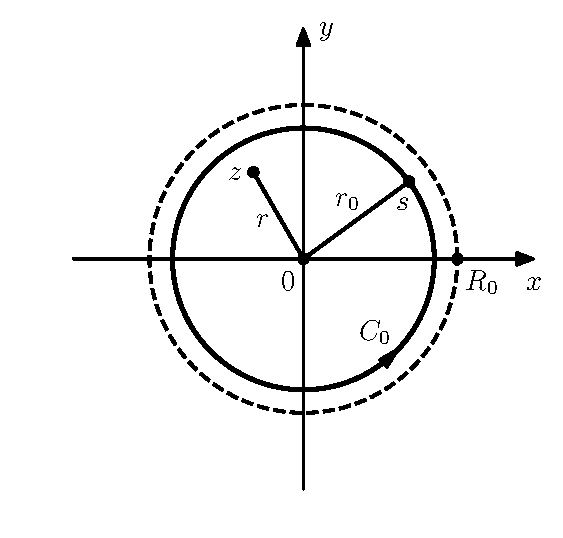
\includegraphics[width=\textwidth]{figuras/taylor_series_proof.pdf}
  \end{minipage}\hfill
  \begin{minipage}[c]{0.48\textwidth}
    \caption{
       Prueba del teorema de Taylor.
    }\label{fig:taylor_series_proof}
  \end{minipage}
\end{figure}

Continuando, se observa que el factor \(1/(s-z)\) del integrando puede escribirse como 
\begin{equation}\label{eq:taylor_series_proof_tmp1}
 \frac{1}{s-z}=\frac{1}{s}\cdot\frac{1}{1-(z/s)}. 
\end{equation}
Además, se sabe del ejemplo de la sección \ref{sec:convergence_of_series} (ver la ecuación \ref{eq:geometric_series_to_N-1}) que 
\[
 \frac{1}{1-z}=\sum_{n=0}^{N-1}z^n+\frac{z^N}{1-z}
 \qquad\qquad\textrm{cuando}\qquad\qquad
 z\neq 1. 
\]
Reemplazando \(z\) por \(z/s\) en esta última identidad, resulta en
\[
 \frac{1}{1-(z/s)}=\sum_{n=0}^{N-1}\frac{z^n}{s^n}+\frac{z^N/s^N}{1-(z/s)},
\]
y sustituyendo este resultado en la ecuación \ref{eq:taylor_series_proof_tmp1} se obtiene que 
\begin{equation}\label{eq:taylor_series_proof_tmp2}
 \frac{1}{s-z}=\sum_{n=0}^{N-1}\frac{z^n}{s^{n+1}}+\frac{z^N}{(s-z)s^N}. 
\end{equation}
Multiplicando esta igualdad por \(f(s)/(2\pi i)\) e integrando ambos lados respecto a \(s\) sobre el contorno \(C_0\), se encuentra que 
\[
 \frac{1}{2\pi i}\int_{C_0}\frac{f(s)}{s-z}\,ds=\sum_{n=0}^{N-1}\left[\frac{1}{2\pi i}\int_{C_0}\frac{f(s)}{s^{n+1}}\,ds\right]z^n+\frac{z^N}{2\pi i}\int_{C_0}\frac{f(s)}{(s-z)s^N}\,ds.
\]
De la ecuación \ref{eq:taylor_series_proof_tmp0} de la fórmula integral de Cauchy, el lado izquierdo de la igualdad es \(f(z)\), y de la ecuación \ref{eq:cauchy_integral_formula_extension_alt} de la extensión de la fórmula integral de Cauchy, el término entre paréntesis rectos es \(f^{(n)}(0)/n!\), considerando que el punto \(z=0\) es interior a \(C_0\). Por lo tanto,
\[
 f(z)=\sum_{n=0}^{N-1}\frac{f^{(n)}(0)}{n!}z^n+\rho_N(z),
\]
donde
\[
 \rho_N(z)=\frac{z^N}{2\pi i}\int_{C_0}\frac{f(s)}{(s-z)s^N}\,ds.
\]
La representación \ref{eq:maclaurin_series_definition} queda probada si
\begin{equation}\label{eq:taylor_series_proof_tmp3}
 \lim_{N\to\infty}\rho_N(z)=0. 
\end{equation}
Para ver que esto es así, se considera que \(|z|=r\) y \(C_0\) tiene radio \(r_0\) con \(r_0>r\). Por lo tanto, si \(s\) es un punto de \(C_0\), se cumple que (ver la sección \ref{sec:triangle_inequality})
\[
 |s-z|\geq||s|-|z||=r_0-r.
\]
En consecuencia, si \(M\) es el valor máximo de \(|f(s)|\) sobre \(C_0\), de la ecuación \ref{eq:contour_integral_upper_bound}), se deduce que
\[
 |\rho_N(z)|\leq\frac{r^N}{2\pi}\times\frac{M}{(r_0-r)r_0^N}\times2\pi r_0=\frac{Mr_0}{r_0-r}\left(\frac{r}{r_0}\right)^N.
\]
Como \(r/r_0<1\), el límite de la ecuación \ref{eq:taylor_series_proof_tmp3} se cumple.

\subsection*{Caso con \(z_0\neq0\)}

Para verificar el teorema cuando el disco de radio \(R_0\) está centrado en un punto \(z_0\) arbitrario, se asume que \(f\) es analítica en \(|z-z_0|<R_0\) y se observa que entonces la función compuesta \(f(z+z_0)\) debe ser analítica en \(|(z+z_0)-z_0|<R_0\). Esta última desigualdad es \(|z|<R_0\), y si se define \(g(z)=f(z+z_0)\), la analiticidad de \(g(z)\) en \(|z|<R_0\) asegura la existencia de la representación en la serie de Maclaurin
\[
 g(z)=\sum_{n=0}^\infty\frac{g^{(n)}(0)}{n!}z^n
 \qquad\qquad\textrm{cuando}\qquad\qquad
 |z|<R_0,
\]
es decir, 
\[
 f(z+z_0)=\sum_{n=0}^\infty\frac{f^{(n)}(z_0)}{n!}z^n
 \qquad\qquad\textrm{cuando}\qquad\qquad
 |z|<R_0, 
\]
Luego de reemplazar \(z\) por \(z-z_0\) en esta ecuación y su condición de validez, se obtiene la expansión en series de Taylor de la ecuación \ref{eq:taylor_series_definition}. 

\section{Ejemplos}\label{sec:taylor_series_examples}

En la sección \ref{sec:series_representation_unicity} se verá que la representación en series de Taylor de una función \(f(z)\) en torno a un punto  \(z_0\) específico es única. Mas precisamente, se mostrará que si
\[
 f(z)=\sum_{n=0}^\infty a_n(z-z_0)^n
\]
para todos los puntos \(z\) interiores a algún círculo centrado en \(z_0\), esta serie de potencias debe ser la serie de Taylor de \(f\) en torno a \(z_0\), independientemente de como se hayan obtenido las constantes. Esta observación permite a menudo encontrar los coeficientes \(a_n\) de la serie de Taylor de forma mas eficiente que aplicando la ecuación \ref{eq:taylor_series_an_definition} del teorema de Taylor.

A continuación se lista la representación en series de Maclaurin de seis funciones, que son útiles debido a que a partir de ellas pueden obtenerse la representación de algunas otras funciones de forma directa.
\begin{gather}
 \frac{1}{1-z}=\sum_{n=0}^\infty z^n=1+z+z^2+\dots
 \qquad\qquad\textrm{cuando}\qquad\qquad
 |z|<1\label{eq:taylor_series_geometric}\\
 e^z=\sum_{n=0}^\infty\frac{z^n}{n!}=1+\frac{z}{1!}+\frac{z^2}{2!}+\dots
 \qquad\qquad\textrm{cuando}\qquad\qquad
 |z|<\infty\label{eq:taylor_series_exponential}\\
 \sen z=\sum_{n=0}^\infty(-1)^n\frac{z^{2n+1}}{(2n+1)!}=z-\frac{z^3}{3!}+\frac{z^5}{5!}-\dots
 \qquad\qquad\textrm{cuando}\qquad\qquad
 |z|<\infty\label{eq:taylor_series_sen}\\
 \cos z=\sum_{n=0}^\infty(-1)^n\frac{z^{2n}}{(2n)!}=1-\frac{z^2}{2!}+\frac{z^4}{4!}-\dots
 \qquad\qquad\textrm{cuando}\qquad\qquad
 |z|<\infty\label{eq:taylor_series_cos}\\
  \senh z=\sum_{n=0}^\infty\frac{z^{2n+1}}{(2n+1)!}=z+\frac{z^3}{3!}+\frac{z^5}{5!}+\dots
 \qquad\qquad\textrm{cuando}\qquad\qquad
 |z|<\infty\label{eq:taylor_series_senh}\\
 \cosh z=\sum_{n=0}^\infty\frac{z^{2n}}{(2n)!}=1+\frac{z^2}{2!}+\frac{z^4}{4!}+\dots
 \qquad\qquad\textrm{cuando}\qquad\qquad
 |z|<\infty\label{eq:taylor_series_cosh}
\end{gather}
En los siguientes ejemplos se derivan algunas de estos resultados. Hay que tener en cuenta que:
\begin{enumerate}
 \item[(\textit{a})] la región de convergencia puede obtenerse antes de calcular la representación en series.
 \item[(\textit{b})] en general hay varias formas razonables de obtener la representación en series.
\end{enumerate}

\paragraph{Ejemplo 1.} Asumiendo que se cumple la representación \ref{eq:taylor_series_sen} (ver una deducción en el ejercicio 7 de la sección \ref{sec:taylor_series_negative_powers}), se mostrará que se cumple la representación \ref{eq:taylor_series_cos}. Empleando diferenciación término a término, que se justificará en la sección \ref{sec:series_integration_differentiation}, se diferencia ambos lados de la identidad \ref{eq:taylor_series_sen},
\[
 \cos z=\sum_{n=0}^\infty\frac{(-1)^n}{(2n+1)!}\frac{d}{dz}z^{2n+1}
  =\sum_{n=0}^\infty(-1)^n\frac{2n+1}{(2n+1)!}z^{2n}
  =\sum_{n=0}^\infty(-1)^n\frac{z^{2n}}{(2n)!}
 \qquad\textrm{cuando}\qquad
 |z|<\infty
\]
En el ejercicio 8 de la sección \ref{sec:taylor_series_negative_powers} se deriva esta serie de Taylor de otras dos formas alternativas.

\paragraph{Ejemplo 2.} Considerando que \(\senh z=-i\sen(iz)\) (ver la ecuación \ref{eq:hyperbolic_trigonometric_relations_2}), empleando la expresión \ref{eq:taylor_series_sen} reemplazando \(z\) por \(iz\), se tiene que 
\begin{align*}
 \senh z&=-i\sum_{n=0}^\infty(-1)^n\frac{(iz)^{2n+1}}{(2n+1)!}\\
  &=\sum_{n=0}^\infty(-1)^ni^{2n+1}(-i)\frac{z^{2n+1}}{(2n+1)!}\\
  &\overset{(a)}{=}\sum_{n=0}^\infty(-1)^n(-1)^ni(-i)\frac{z^{2n+1}}{(2n+1)!}\\
  &\overset{(b)}{=}\sum_{n=0}^\infty\frac{z^{2n+1}}{(2n+1)!}
 \qquad\qquad\textrm{cuando}\qquad\qquad
 |z|<\infty,
\end{align*}
que es la expresión \ref{eq:taylor_series_senh}. En la deducción, en \((a)\) se empleó que  
\[
 i^{2n+1}=i^{2n}i=(i^2)^ni=(-1)^ni
\]
y en \((b)\) que \((-1)^n(-1)^n=(-1)^{2n}=1\) y que \(i(-i)=1\).
 
La deducción de las demás expresiones puede encontrarse en \cite{brown2013complex}, o en ciertos casos es similar a la realizada en algunos ejercicios de la sección \ref{sec:taylor_series_negative_powers}.

\section{Potencias negativas de \texorpdfstring{\((z-z_0)\)}{(z-z0)}}\label{sec:taylor_series_negative_powers}

Si una función \(f\) falla en ser analítica en \(z_0\) no puede aplicarse el teorema de Taylor. Sin embargo, a menudo es posible obtener una representación en series para \(f(z)\), la cual involucra tanto potencias positivas como potencias negativas de \(z-z_0\). Dichas series son extremadamente importantes y se tratan en la sección siguiente. Usualmente pueden obtenerse empleando alguna de las series de Maclaurin listadas al comienzo de la sección \ref{sec:taylor_series_examples}. Como anticipo, a continuación se incluye un ejemplo, y algunos ejemplos mas se incluyen en la sección de ejercicios.

\paragraph{Ejemplo.} Empleando la serie de Maclaurin \ref{eq:taylor_series_exponential}
\[
 e^z=\sum_{n=0}^\infty\frac{z^n}{n!}
 \qquad\qquad\textrm{cuando}\qquad\qquad
 |z|<\infty
\]
puede verse que 
\[
 \frac{e^{-z}}{z^2}=\frac{1}{z^2}\sum_{n=0}^\infty(-1)^n\frac{z^n}{n!}=\sum_{n=0}^\infty(-1)^n\frac{z^{n-2}}{n!}
 =\frac{1}{z^2}-\frac{1}{z}+\sum_{n=2}^\infty(-1)^n\frac{z^{n-2}}{n!}
\]
resultando en que 
\[
 \frac{e^{-z}}{z^2}=\frac{1}{z^2}-\frac{1}{z}+\sum_{n=0}^\infty(-1)^n\frac{z^{n}}{(n+2)!}
 \qquad\qquad\textrm{cuando}\qquad\qquad
 0<|z|<\infty.
\]

\subsection*{Ejercicios}

\subsubsection*{Ejercicio 1}

Obtener la representación en series de Maclaurin de
\[
 z\cosh(z^2)=\sum_{n=0}^\infty\frac{z^{4n+1}}{(2n)!}
 \qquad\qquad\textrm{cuando}\qquad\qquad
 |z|<\infty.
\]

\paragraph{Solución.} Partiendo de la representación en series \ref{eq:taylor_series_cosh} sustituyendo \(z\) por \(z^2\) se tiene que  
\[
 z\cosh(z^2)=z\sum_{n=0}^\infty\frac{z^{4n}}{(2n)!}=\sum_{n=0}^\infty\frac{z^{4n+1}}{(2n)!}
 \qquad\qquad\textrm{cuando}\qquad\qquad
 |z|<\infty.
\]

\subsubsection*{Ejercicio 2}

Obtener las series de Taylor de
\[
 e^z=e\sum_{n=0}^\infty\frac{(z-1)^n}{n!}
 \qquad\qquad\textrm{cuando}\qquad\qquad
 |z-1|<\infty
\]
para la función \(f(z)=e^z\) de las siguientes formas:
\begin{enumerate}
 \item[(\textit{a})] empleando \(f^{(n)}(1)\) con \(n=0,\,1,\,2,\,\dots\).
 \item[(\textit{b})] escribiendo \(e^z=e^{z-1}e\).
\end{enumerate}

\paragraph{Solución.}

\begin{enumerate}
 \item[(\textit{a})] Se empleará la definición \ref{eq:taylor_series_definition} de series de potencias con \(z_0=1\). Considerando que \(f^{(n)}(z)=e^z\) y por lo tanto \(f^{(n)}(1)=e\), se tiene que 
 \[
  e^z=\sum_{n=0}^\infty\frac{e}{n!}(z-1)^n=e\sum_{n=0}^\infty\frac{(z-1)^n}{n!}
  \qquad\qquad\textrm{en}\qquad\qquad
  |z-1|<\infty
 \]
 \item[(\textit{b})] Se tiene que 
 \[
  e^z=ee^{z-1}=e\sum_{n=0}^\infty\frac{(z-1)^n}{n!}
  \qquad\qquad\textrm{en}\qquad\qquad
  |z-1|<\infty,
 \]
 donde en la última igualdad se empleó la ecuación \ref{eq:taylor_series_exponential} de la representación en series de Maclaurin de \(e^z\) reemplazando \(z\) por \(z-1\).
\end{enumerate}

\subsubsection*{Ejercicio 3}

Encontrar la expansión en series de Maclaurin de la función
\[
 f(z)=\frac{z}{z^4+4}=\frac{z}{4}\cdot\frac{1}{1+(z^4/4)}.
\]

\paragraph{Solución.} Se observa que 
\begin{align*}
 \frac{z}{z^4+4}&=\frac{z}{4}\cdot\frac{1}{1+(z^4/4)}\\
 &\overset{(a)}{=}\frac{z}{4}\sum_{n=0}^\infty\left(-\frac{z^4}{4}\right)^n\\
 &=\frac{z}{4}\sum_{n=0}^\infty(-1)^n\frac{z^{4n}}{4^n}\\
 &=\frac{z}{2^2}\sum_{n=0}^\infty(-1)^n\frac{z^{4n}}{2^{2n}}\\
 &=\sum_{n=0}^\infty(-1)^n\frac{z^{4n+1}}{2^{2n+2}}
 \qquad\qquad\textrm{en}\qquad\qquad
  |z|<\sqrt{2},
\end{align*}
donde en \((a)\) se empleó la representación en series de Maclaurin de la ecuación \ref{eq:taylor_series_geometric} reemplazando \(z\) por \(-z^4/4\). Observar que al realizar dicho reemplazo, la condición de validez en la representación \ref{eq:taylor_series_geometric} es
\[
 \left|-\frac{z^4}{4}\right|<1
 \qquad\Leftrightarrow\qquad 
 |z^4|<4
 \qquad\Leftrightarrow\qquad 
 |z|^4<4
 \qquad\Leftrightarrow\qquad 
 |z|<\sqrt[4]{4}
 \qquad\Leftrightarrow\qquad 
 |z|<\sqrt{2}.
\]

\subsubsection*{Ejercicio 4}

Con la ayuda de la identidad (ver la ecuación \ref{eq:sin_and_cosine_double_angle})
\[
 \cos z=-\sen\left(z-\dfrac{\pi}{2}\right)
\]
expandir \(\cos z\) en series de Taylor en torno a \(z_0=\pi/2\).

\paragraph{Solución.} Se ve que 
\begin{align*}
 \cos z&=-\sen\left(z-\dfrac{\pi}{2}\right)\\
  &\overset{(a)}{=}-\sum_{n=0}^\infty(-1)^n\frac{\left(z-\pi/2\right)^{2n+1}}{(2n+1)!}\\
  &=\sum_{n=0}^\infty(-1)^{n+1}\frac{\left(z-\pi/2\right)^{2n+1}}{(2n+1)!}
  \qquad\qquad\textrm{cuando}\qquad\qquad
 |z-\pi/2|<\infty,
\end{align*}
donde en \((a)\) se empleó la representación \ref{eq:taylor_series_sen} en series de Maclaurin de \(\sen z\) reemplazando \(z\) por \(z-\pi/2\). 

\subsubsection*{Ejercicio 5}

Emplear la identidad \(\senh(z+\pi i)=-\senh z\), verificada en el ejercicio 7(\textit{a}) de la sección \ref{sec:hyperbolic_functions}, y el hecho de que \(\senh z\) es periódica de período \(2\pi i\) para encontrar las series de Taylor de \(\senh z\) en torno al punto \(\pi i\).

\paragraph{Solución.} Se ve que 
\begin{align*}
 \senh z&\overset{(a)}{=}-\senh(z+\pi i)\\
  &\overset{(b)}{=}-\senh(z-\pi i)\\
  &\overset{(c)}{=}-\sum_{n=0}^\infty\frac{(z-\pi i)^{2n+1}}{(2n+1)!}
 \qquad\qquad\textrm{cuando}\qquad\qquad
 |z-\pi i|<\infty
\end{align*}
donde en \((a)\) se empleó el resultado del ejercicio 7(\textit{a}) de la sección \ref{sec:hyperbolic_functions}, en \((b)\) se consideró que \(\senh z\) es periódica de período \(2\pi i\), como se comprobó en la sección la sección \ref{sec:hyperbolic_functions}, y en \((c)\) se empleó la representación 
\ref{eq:taylor_series_senh} en series de Taylor de \(\senh z\) reemplazando \(z\) por \(z-\pi i\).

\subsubsection*{Ejercicio 6}

¿Cuál es el mayor círculo dentro del cual las series de Maclaurin de la función \(\tanh z\) converge a \(\tanh z\)? Escribir los dos primeros términos no nulos de dichas series.

\paragraph{Solución.} La función 
\[
 \tanh z=\frac{\senh z}{\cosh z}
\]
tiene puntos singulares en \(\cosh z=0\), y como indica el teorema de la sección \ref{sec:hyperbolic_functions},
\[
 \cosh z=0
 \qquad\textrm{si y solo si}\qquad
 z=\left(\frac{\pi}{2}+n\pi\right)i
 \qquad\textrm{con}\qquad 
 n=0,\,\pm1,\,\pm2,\,\dots.
\]
Por lo tanto, el mayor círculo en donde las series de Maclaurin converge es \(|z|<\pi/2\).

Para calcular los dos primeros términos no nulos delas series de Maclaurin, se empleará la ecuación \ref{eq:taylor_series_definition} con \(z_0=0\). Considerando las derivadas de las funciones hiperbólicas de la ecuación \ref{eq:hyperbolic_functions_reciprocal_derivatives}, la derivada primera es
\[
 \tanh'z=\sech^2z=\frac{1}{\cosh^2z}, 
\]
la derivada segunda es
\[
 \tanh''z=(\sech^2z)'=2\sech z(-\sech z\tanh z)=-2\sech^2z\tanh z,
\]
y la derivada tercera queda
\begin{align*}
 \tanh'''z&=(-2\sech^2z\tanh z)'\\
  &=-2(-2\sech^2z\tanh^2z+\sech^4z)\\
  &=2\sech^2z(2\tanh^2-\sech^2z)\\
  &=\frac{2}{\cosh^2z}\left(\frac{2\senh^2z}{\cosh^2z}-\frac{1}{\cosh^2z}\right)\\
  &=\frac{2(2\senh^2z-1)}{\cosh^2z}.
\end{align*}
A partir de estos resultados y considerando que \(\senh0=0\) y \(\cosh0=1\), se tiene que 
\[
 \tanh0=0,
 \qquad\qquad
 \tanh'0=1,
 \qquad\qquad 
 \tanh''0=0
 \qquad\qquad\textrm{y}\qquad\qquad 
 \tanh'''0=-2.
\]
Sustituyendo estos resultados en la ecuación \ref{eq:taylor_series_definition}, se obtiene que 
\begin{align*}
 \tanh z&=0+\frac{1}{1!}z+\frac{0}{2!}z^2+\frac{(-2)}{3!}z^3+\dots\\
   &=z-\frac{z^3}{3}+\dots
   \qquad\qquad\textrm{cuando}\qquad\qquad
 |z|<\frac{\pi}{2}.
\end{align*}

\subsubsection*{Ejercicio 7}

Mostrar que si \(f(z)=\sen z\), entonces
\[
 f^{(2n)}(0)=0
 \qquad\qquad\textrm{y}\qquad\qquad
 f^{(2n+1)}(0)=(-1)^n,
 \qquad\qquad 
 n=0,\,1,\,2,\,\dots.
\]
Brindar entonces una deducción alternativa para las series de Maclaurin \ref{eq:taylor_series_sen}.

\paragraph{Solución.} Observando que 
\[
 f(z)=\sen z,\qquad 
 f'(z)=\cos z,\qquad
 f''(z)=-\sen z,\qquad
 f'''(z)=-\cos z,\qquad
 f^{(4)}(z)=\sen z
\]
y así sucesivamente, puede verse que esto se generaliza como
\[
 f^{(2n)}(z)=(-1)^n\sen z
 \qquad\qquad\textrm{y}\qquad\qquad
 f^{(2n+1)}(z)=(-1)^n\cos z,
 \qquad\qquad 
 n=0,\,1,\,2,\,\dots,
\]
y por lo tanto
\[
 f^{(2n)}(0)=0
 \qquad\qquad\textrm{y}\qquad\qquad
 f^{(2n+1)}(0)=(-1)^n,
 \qquad\qquad 
 n=0,\,1,\,2,\,\dots.
\]
Sustituyendo este resultado en la ecuación \ref{eq:taylor_series_definition} se obtiene que 
\[
 \sen z=\sum_{n=0}^\infty(-1)^n\frac{z^{2n+1}}{(2n+1)!}
 \qquad\qquad\textrm{cuando}\qquad\qquad
 |z|<\infty.
\]

\subsubsection*{Ejercicio 8}

Derivar las series de Maclaurin \ref{eq:taylor_series_cos} de la función \(\cos z\) mediante:
\begin{enumerate}
 \item[(\textit{a})] el uso de la definición 
 \[
  \cos z=\frac{e^{iz}+e^{-iz}}{2}
 \]
 dada en la ecuación \ref{eq:sin_and_cosine_definition} y recurriendo a la series de Maclaurin de \(e^z\) dada por la ecuación \ref{eq:taylor_series_exponential};
 \item[(\textit{b})] mostrando que 
 \[
  f^{(2n)}(0)=(-1)^n
  \qquad\qquad\textrm{y}\qquad\qquad
  f^{(2n+1)}(0)=0,
  \qquad\qquad 
  n=0,\,1,\,2,\,\dots.
 \]
\end{enumerate}

\paragraph{Solución.} 
\begin{enumerate}
 \item[(\textit{a})] Reemplazando \(z\) por \(iz\) y \(-iz\) en la serie de Maclaurin \ref{eq:taylor_series_exponential} y sustituyendo los resultados en la ecuación \ref{eq:sin_and_cosine_definition} de la definición de \(\cos z\), se tiene que 
 \begin{align*}
  \cos z&=\frac{1}{2}\left[\sum_{n=0}^\infty\frac{(iz)^n}{n!}+\sum_{n=0}^\infty\frac{(-iz)^n}{n!}\right]\\
   &=\frac{1}{2}\sum_{n=0}^\infty[1+(-1)^n]\frac{(iz)^n}{n!}\\
   &\overset{(a)}{=}\frac{1}{2}\sum_{n=0}^\infty2\frac{(iz)^{2n}}{(2n)!}\\
   &=\sum_{n=0}^\infty i^{2n}\frac{z^{2n}}{(2n)!}\\
   &\overset{(b)}{=}\sum_{n=0}^\infty(-1)^n\frac{z^{2n}}{(2n)!}
   \qquad\qquad\textrm{cuando}\qquad\qquad
   |z|<\infty,
 \end{align*}
 donde en \((a)\) se consideró que 
 \[
  1+(-1)^n=
  \left\{ 
  \begin{array}{ll}
   2 & \textrm{si }n\textrm{ es par}\\
   0 & \textrm{si }n\textrm{ es impar},
  \end{array}\right.
 \]
 y por lo tanto, puede reemplazarse \(n\) por \(2n\), y en \((b)\) se tuvo en cuenta que \(i^{2n}=(i^2)^n=(-1)^n\).
 \item[(\textit{b})]  Observando que 
\[
 f(z)=\cos z,\qquad 
 f'(z)=-\sen z,\qquad
 f''(z)=-\cos z,\qquad
 f'''(z)=\sen z,\qquad
 f^{(4)}(z)=\cos z
\]
y así sucesivamente, puede verse que esto se generaliza como
\[
 f^{(2n)}(z)=(-1)^n\cos z
 \qquad\qquad\textrm{y}\qquad\qquad
 f^{(2n+1)}(z)=(-1)^{n+1}\sen z,
 \qquad\qquad 
 n=0,\,1,\,2,\,\dots,
\]
y por lo tanto
\[
 f^{(2n)}(0)=(-1)^n
 \qquad\qquad\textrm{y}\qquad\qquad
 f^{(2n+1)}(0)=0,
 \qquad\qquad 
 n=0,\,1,\,2,\,\dots.
\]
Sustituyendo este resultado en la ecuación \ref{eq:taylor_series_definition} se obtiene que 
\[
 \sen z=\sum_{n=0}^\infty(-1)^n\frac{z^{2n}}{(2n)!}
 \qquad\qquad\textrm{cuando}\qquad\qquad
 |z|<\infty.
\]
\end{enumerate}

\subsubsection*{Ejercicio 9}

Emplear la expresión \ref{eq:taylor_series_sen} de \(\sen z\) para encontrar las series de Maclaurin de
\[
 f(z)=\sen(z^2)
\]
e indicar como se obtiene que 
\[
 f^{(4n)}(0)=0
 \qquad\qquad\textrm{y}\qquad\qquad
 f^{(2n+1)}(0)=0,
 \qquad\qquad 
 n=0,\,1,\,2,\,\dots.
\]

\paragraph{Solución.} Reemplazando \(z\) por \(z^2\) en la representación \ref{eq:taylor_series_sen} de \(\sen z\), se  obtiene que 
\[
 \sen(z^2)=\sum_{n=0}^\infty(-1)^n\frac{z^{4n+2}}{(2n+1)!}=z^2-\frac{z^6}{3!}+\frac{z^{10}}{5!}-\frac{z^{14}}{7!}+\cdots
 \qquad\qquad\textrm{cuando}\qquad\qquad
 |z|<\infty.
\]
Considerando que la representación en series de Taylor es única, asociando los términos de esta expresión con la definición \ref{eq:taylor_series_definition} de series de Taylor, se observa que 
\[
 \sum_{k=0}^\infty\frac{f^{(k)}(0)}{k!}z^k=\sum_{n=0}^\infty(-1)^n\frac{z^{4n+2}}{(2n+1)!},
\]
e igualando los coeficientes de los términos de igual grado de los polinomios, se cumple que \(f^{(k)}(0)=0\) cuando \(k=2n+1\) o \(k=4n\), es decir, cuando \(k\) es impar o múltiplo de cuatro, que es lo que se quería mostrar. Además, cuando \(k=4n+2\), se cumple que
\[
 \frac{f^{(4n+2)}(0)}{(4n+2)!}=\frac{(-1)^n}{(2n+1)!}
 \qquad\qquad 
 n=0,\,1,\,2,\,\dots,
\]
o
\[
 f^{(4n+2)}(0)=(-1)^n\frac{(4n+2)!}{(2n+1)!}
 \qquad\qquad 
 n=0,\,1,\,2,\,\dots.
\]

\subsubsection*{Ejercicio 10}

Derivar las expansiones 
\begin{enumerate}
 \item[(\textit{a})] \(\displaystyle\frac{\senh z}{z^2}=\frac{1}{z}+\sum_{n=0}^\infty\frac{z^{2n+1}}{(2n+3)!}
 \qquad\textrm{cuando}\qquad\qquad
 0<|z|<\infty\);
 \item[(\textit{b})] \(\displaystyle\frac{\sen z}{z^4}=\frac{1}{z^2}-\frac{z^2}{3!}+\frac{z^6}{5!}-\frac{z^{10}}{7!}+\cdots
 \qquad\textrm{cuando}\qquad\qquad
 0<|z|<\infty\).
\end{enumerate}

\paragraph{Solución.} 
\begin{enumerate}
 \item[(\textit{a})] Partiendo de la expresión \ref{eq:taylor_series_senh} de la serie de Maclaurin de \(\senh z\) se observa que 
 \begin{align*}
  \frac{\senh z}{z^2}&=\frac{1}{z^2}\sum_{n=0}^\infty\frac{z^{2n+1}}{(2n+1)!}\\
    &=\frac{1}{z^2}\left[z+\frac{z^3}{3!}+\frac{z^5}{5!}+\dots\right]\\
    &=\frac{1}{z}+\frac{z}{3!}+\frac{z^3}{5!}+\dots\\
    &=\frac{1}{z}+\sum_{n=0}^\infty\frac{z^{2n+1}}{(2n+3)!}
     \qquad\qquad\textrm{cuando}\qquad\qquad
     0<|z|<\infty.
 \end{align*}
 \item[(\textit{b})] Partiendo de la serie de Maclaurin de \(\sen(z^2)\) obtenida en el ejercicio 9, se ve que 
 \begin{align*}
  \frac{\sen(z^2)}{z^4}&=\frac{1}{z^4}\sum_{n=0}^\infty(-1)^n\frac{z^{4n+2}}{(2n+1)!}\\
   &=\frac{1}{z^4}\left[z^2-\frac{z^6}{3!}+\frac{z^{10}}{5!}-\frac{z^{14}}{7!}+\cdots\right]\\
   &=\frac{1}{z^2}-\frac{z^2}{3!}+\frac{z^6}{5!}-\frac{z^{10}}{7!}+\cdots\\
   &=\frac{1}{z^2}+\sum_{n=1}^\infty(-1)^n\frac{z^{4n-2}}{(2n+1)!}\\
   &\overset{(a)}{=}\frac{1}{z^2}+\sum_{m=0}^\infty(-1)^{m+1}\frac{z^{4(m+1)-2}}{[2(m+1)+1]!}\\
   &=\frac{1}{z^2}+\sum_{n=0}^\infty(-1)^{n+1}\frac{z^{4n+2}}{(2n+3)!}
  \qquad\qquad\textrm{cuando}\qquad\qquad
  0<|z|<\infty,
 \end{align*}
 donde en \((a)\) se realizó el cambio de variable \(n=m+1\).
\end{enumerate} 
 
\subsubsection*{Ejercicio 11} 
 
Mostrar que cuando \(0<|z|<4\),
\[
 \frac{1}{4z-z^2}=\frac{1}{4z}+\sum_{n=0}^\infty\frac{z^n}{4^{n+2}}.
\]

\paragraph{Solución.} 
\begin{align*}
 \frac{1}{4z-z^2}&=\frac{1}{4z}\cdot\frac{1}{1-z/4}\\
  &\overset{(a)}{=}\frac{1}{4z}\sum_{n=0}^\infty\frac{z^n}{4^n}\\
  &=\frac{1}{4z}\left[1+\sum_{n=1}^\infty\frac{z^n}{4^n}\right]\\
  &=\frac{1}{4z}+\sum_{n=1}^\infty\frac{z^{n-1}}{4^{n+1}}\\
  &\overset{(b)}{=}\frac{1}{4z}+\sum_{m=0}^\infty\frac{z^m}{4^{m+2}}
  \qquad\qquad\textrm{cuando}\qquad\qquad
  0<|z|<4,
\end{align*}
donde en \((a)\) se empleó la representación en series de Maclaurin de la ecuación \ref{eq:taylor_series_geometric} sustituyendo \(z\) por \(z/4\) y por lo tanto la región de convergencia es el disco \(|z/4|<1\) y en \((b)\) se realizó el cambio de variable \(n=m+1\).
 
\section{Series de Laurent}\label{sec:laurent_series} 
 
Se pasa ahora a la declaración del teorema de Laurent, que permite expandir una función \(f(z)\) en series que involucran potencias positivas y negativas de \((z-z_0)\) cuando la función falla en ser analítica en \(z_0\). 
 
\paragraph{Teorema.} Supóngase que una función \(f\) es analítica en un dominio anular \(R_1<|z-z_0|<R_2\) centrado en \(z_0\), y sea \(C\) cualquier contorno cerrado simple orientado positivamente que rodea a \(z_0\) y pertenece a dicho dominio, como se muestra en la figura \ref{fig:laurent_theorem}. Entonces, en cada punto en el dominio, \(f(z)\) tiene la representación en series
\begin{equation}\label{eq:laurent_series_definition}
 f(z)=\sum_{n=0}^\infty a_n(z-z_0)^n+\sum_{n=1}^\infty\frac{b_n}{(z-z_0)^n}
 \qquad\qquad\textrm{en}\qquad\qquad
 R_1<|z-z_0|<R_2,
\end{equation}
donde
\begin{equation}\label{eq:laurent_series_an_definition}
 a_n=\frac{1}{2\pi i}\int_C\frac{f(z)}{(z-z_0)^{n+1}}\,dz
 \qquad\qquad\textrm{con}\qquad\qquad
 n=0,\,1,\,2,\,\dots
\end{equation}
y
\begin{equation}\label{eq:laurent_series_bn_definition}
 b_n=\frac{1}{2\pi i}\int_C\frac{f(z)}{(z-z_0)^{-n+1}}\,dz
 \qquad\qquad\textrm{con}\qquad\qquad
 n=1,\,2,\,\dots
\end{equation}
\begin{figure}[!htb]
  \begin{minipage}[c]{0.5\textwidth}
    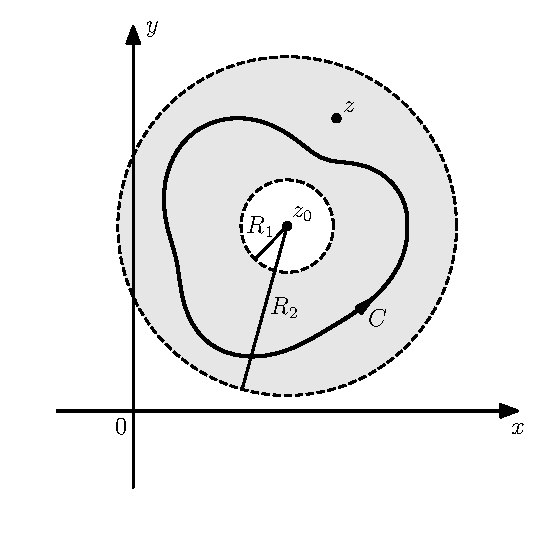
\includegraphics[width=\textwidth]{figuras/laurent_theorem.pdf}
  \end{minipage}\hfill
  \begin{minipage}[c]{0.4\textwidth}
    \caption{
       Teorema de Laurent. Dominio anular centrado en \(z_0\) donde \(f\) es analítica y contorno \(C\) contenido en dicho dominio.
    }\label{fig:laurent_theorem}
  \end{minipage}
\end{figure}

Notar como reemplazando \(n\) por \(-n\) en la segunda representación en series en la ecuación \ref{eq:laurent_series_definition} permite escribir dicha serie como
\[
 \sum_{n=-\infty}^{-1}\frac{b_{-n}}{(z-z_0)^{-n}}
\]
donde
\[
 b_{-n}=\frac{1}{2\pi i}\int_C\frac{f(z)}{(z-z_0)^{n+1}}\,dz
 \qquad\qquad\textrm{con}\qquad\qquad
 n=-1,\,-2,\,\dots.
\]
De esta forma \(R_2\),
\[
 f(z)=\sum_{n=-\infty}^{-1}b_{-n}(z-z_0)^n+\sum_{n=0}^\infty a_n(z-z_0)^n
 \qquad\qquad\textrm{en}\qquad\qquad
 R_1<|z-z_0|<R_2.
\]
Definiendo
\[
 c_n=
 \left\{
 \begin{array}{lll}
  b_{-n} &\textrm{cuando} &n\leq-1\\
  a_n &\textrm{cuando}&n\geq0,
 \end{array}
 \right.
\]
esto queda
\begin{equation}\label{eq:laurent_series_definition_alt}
 f(z)=\sum_{n=-\infty}^\infty c_n(z-z_0)^n
 \qquad\qquad\textrm{en}\qquad\qquad
 R_1<|z-z_0|<R_2, 
\end{equation}
donde
\begin{equation}\label{eq:laurent_series_definition_alt_cn}
 c_n=\frac{1}{2\pi i}\int_C\frac{f(z)}{(z-z_0)^{n+1}}\,dz
 \qquad\qquad\textrm{con}\qquad\qquad
 n=0,\,\pm1,\,\pm2,\,\dots. 
\end{equation}
Tanto en las formas de las ecuaciones \ref{eq:laurent_series_definition} o \ref{eq:laurent_series_definition_alt}, la representación de \(f(z)\) se llama \emph{series de Laurent}.

Observar que el integrando en la ecuación \ref{eq:laurent_series_bn_definition} puede escribirse como \(f(z)(z-z_0)^{n-1}\). Por lo tanto, es claro que si \(f\) es en realidad analítica en el disco \(|z-z_0|<R_2\), este  integrando también lo es, y todos los coeficientes \(b_n\) son nulos (ver la sección \ref{sec:cauchy_goursat_theorem}). Además, como (ver la sección \ref{sec:cauchy_integral_formula_extension})
\[
 a_n=\frac{1}{2\pi i}\int_C\frac{f(z)}{(z-z_0)^{n+1}}\,dz=\frac{f^{(n)}(z_0)}{n!}
 \qquad\qquad\textrm{con}\qquad\qquad
 n=0,\,1,\,2,\,\dots,
\]
la expansión \ref{eq:laurent_series_definition} se reduce a las series de Taylor en torno a \(z_0\).

Si \(f\) falla en ser analítica en \(z_0\) pero es analítica en el resto del disco \(|z-z_0|<R_2\), el radio \(R_1\) puede elegirse arbitrariamente pequeño. Por lo tanto, la representación \ref{eq:laurent_series_definition} es válida en el disco perforado \(0<|z-z_0|<R_2\). De forma similar, si \(f\) es analítica en todo el plano finito exterior al círculo \(|z-z_0|=R_1\) la condición de validez es \(R_1<|z-z_0|<\infty\). Notar que si \(f\) es analítica en todos lados en el plano finito excepto el punto \(z_0\), la representación \ref{eq:laurent_series_definition} es válida en todos los puntos de analiticidad, es decir, en \(0<|z-z_0|<\infty\).

Se probará el teorema de Laurent cuando \(z_0=0\), que significa que el anillo está centrado en el origen. La verificación del teorema cunado \(z_0\) es arbitrario es consecuencia inmediata de lo anterior.

\section{Prueba del teorema de Laurent}

Al igual que en el teorema de Taylor, la prueba se dividirá en dos partes, primero considerando el caso en que \(z_0=0\) y luego cuando \(z_0\) es cualquier otro punto en el plano finito.

\subsection*{Caso con \texorpdfstring{\(z_0=0\)}{z0=0}}

Se comienza la prueba construyendo una región anular \(r_1<|z|<r_2\) contenida en el dominio \(R_1<|z|<R_2\) y cuyo interior contiene tanto al punto \(z\) como al contorno \(C\), como se muestra en la figura \ref{fig:laurent_theorem_proof}. Se denotará como \(C_1\) y \(C_2\) a los círculos \(|z|=r_1\) y \(|z|=r_2\) respectivamente, asignándoles orientación positiva. Observar que \(f\) es analítica sobre \(C_1\) y \(C_2\) así como en el dominio anular entre ellos. 
\begin{figure}[!htb]
  \begin{minipage}[c]{0.5\textwidth}
    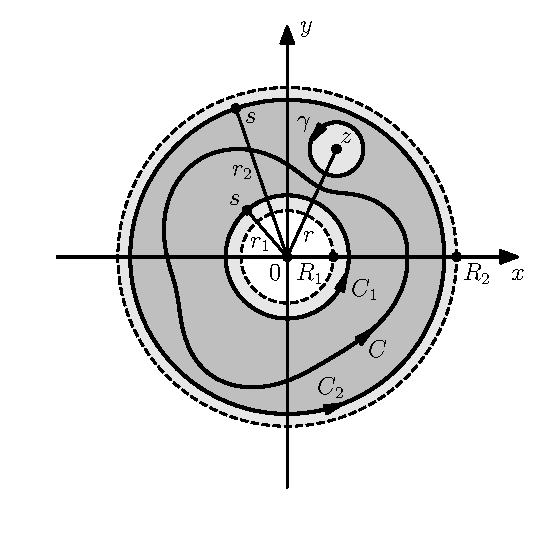
\includegraphics[width=\textwidth]{figuras/laurent_theorem_proof.pdf}
  \end{minipage}\hfill
  \begin{minipage}[c]{0.4\textwidth}
    \caption{
       Prueba del teorema de Laurent con \(z_0=0\).
    }\label{fig:laurent_theorem_proof}
  \end{minipage}
\end{figure}

Luego, se construye un círculo \(\gamma\) centrado en \(z\) orientado positivamente y suficientemente pequeño de forma de estar contenido en la región anular \(r_1<|z|<r_2\). Los círculos \(C_2\), \(C_1\) y \(\gamma\) forman una región múltiplemente conectada, como se muestra en la figura \ref{fig:laurent_theorem_proof}. De la adaptación del teorema de Cauchy-Goursat a integrales de funciones analíticas sobre la frontera de dominios múltiplemente conectados presentada en la sección \ref{sec:multiply_connected_domains}, se cumple que (ver la ecuación \ref{eq:cauchy_goursat_theorem_multiply_conected_extension})
\[
 \int_{C_2}\frac{f(s)}{s-z}\,ds-\int_{C_1}\frac{f(s)}{s-z}\,ds-\int_{\gamma}\frac{f(s)}{s-z}\,ds=0.
\]
Observar que se consideró que \(f(s)/(s-z)\) es analítica en el interior del dominio múltiplemente conectado, ya que el punto singular \(s=z\) no pertenece al dominio. Pero, de acuerdo a la ecuación \ref{eq:cauchy_integral_formula} de la fórmula integral de Cauchy, la tercera integral es \(2\pi if(z)\), y por lo tanto,
\begin{equation}\label{eq:laurent_theorem_proof_tmp2}
 f(z)=\frac{1}{2\pi i}\int_{C_2}\frac{f(s)}{s-z}\,ds+\frac{1}{2\pi i}\int_{C_1}\frac{f(s)}{z-s}\,ds. 
\end{equation}
Notar que el cambio de signo en la segunda integral se compensó con el cambio de signo del denominador del integrando.

Continuando, el factor \(1/(s-z)\) en la primera integral, como indica la ecuación \ref{eq:taylor_series_proof_tmp2} deducida en la prueba del teorema de Taylor, puede escribirse como
\begin{equation}\label{eq:laurent_theorem_proof_tmp0}
 \frac{1}{s-z}=\sum_{n=0}^{N-1}\frac{z^n}{s^{n+1}}+\frac{z^N}{(s-z)s^N}. 
\end{equation}
De forma análoga, intercambiando \(s\) y \(z\) en esta última identidad, el factor \(1/(z-s)\) en la segunda integral puede escribirse como
\begin{align*}
 \frac{1}{z-s}&=\sum_{n=0}^{N-1}\frac{s^n}{z^{n+1}}+\frac{s^N}{(z-s)z^N}\\
   &=\sum_{n=0}^{N-1}\frac{1}{s^{-n}}\cdot\frac{1}{z^{n+1}}+\frac{1}{z^N}\cdot\frac{s^N}{z-s},
\end{align*}
y realizando el cambio de variable \(m=n+1\) se obtiene que 
\begin{equation}\label{eq:laurent_theorem_proof_tmp1}
 \frac{1}{z-s}=\sum_{m=1}^N\frac{1}{s^{-m+1}}\cdot\frac{1}{z^m}+\frac{1}{z^N}\cdot\frac{s^N}{z-s}. 
\end{equation}
Multiplicando las ecuaciones \ref{eq:laurent_theorem_proof_tmp0} y \ref{eq:laurent_theorem_proof_tmp1} por \(f(s)/2\pi i\) e integrando ambos lados de cada ecuación resultante respecto a \(s\) sobre \(C_2\) y \(C_1\) respectivamente se obtiene que 
\[
 \frac{1}{2\pi i}\int_{C_2}\frac{f(s)}{s-z}\,ds=\sum_{n=0}^{N-1}\underbrace{\vphantom{\sum_{n=0}^{N-1}}\frac{1}{2\pi i}\int_{C_2}\frac{f(s)}{s^{n+1}}\,ds}_{\displaystyle a_n}\cdot z^n+\underbrace{\vphantom{\sum_{n=0}^{N-1}}\frac{z^N}{2\pi i}\int_{C_2}\frac{f(s)}{(s-z)s^N}\,ds}_{\displaystyle\rho_N(z)}
\]
y
\[
 \frac{1}{2\pi i}\int_{C_1}\frac{f(s)}{z-s}\,ds=\sum_{n=1}^N\underbrace{\vphantom{\sum_{n=0}^{N-1}}\frac{1}{2\pi i}\int_{C_1}\frac{f(s)}{s^{-n+1}}\,ds}_{\displaystyle b_n}\cdot\frac{1}{z^n}+\underbrace{\vphantom{\sum_{n=0}^{N-1}}\frac{1}{2\pi iz^N}\int_{C_1}\frac{f(s)s^N}{z-s}\,ds}_{\displaystyle\sigma_N(z)}.
\]
Sustituyendo estos resultados en la ecuación \ref{eq:laurent_theorem_proof_tmp2} resulta en
\begin{equation}\label{eq:laurent_theorem_proof_tmp3}
 f(z)=\sum_{n=0}^{N-1}a_nz^n+\rho_N(z)+\sum_{n=1}^N\frac{b_n}{z^n}+\sigma_N(z), 
\end{equation}
donde los números \(a_n\) con \(n=0,\,1,\,\dots,\,N-1\) y \(b_n\) con \(n=1,\,2,\,\dots,\,N\) están dados por las ecuaciones 
\begin{equation}\label{eq:laurent_theorem_proof_an_bn}
 a_n=\frac{1}{2\pi i}\int_{C_2}\frac{f(s)}{s^{n+1}}\,ds
 \qquad\qquad\textrm{y}\qquad\qquad
 b_n=\frac{1}{2\pi i}\int_{C_1}\frac{f(s)}{s^{-n+1}}\,ds 
\end{equation}
y donde
\[
 \rho_N(z)=\frac{z^N}{2\pi i}\int_{C_2}\frac{f(s)}{(s-z)s^N}\,ds
 \qquad\qquad\textrm{y}\qquad\qquad
 \sigma_N(z)=\frac{1}{2\pi iz^N}\int_{C_1}\frac{f(s)s^N}{z-s}\,ds.
\]
Cuando \(N\) tiende a \(\infty\), la ecuación \ref{eq:laurent_theorem_proof_tmp3} toma la forma apropiada de las series de Laurent \ref{eq:laurent_series_definition} en el dominio \(R_1<|z|<R_2\) si se cumple que 
\[
 \lim_{N\to\infty}\rho_N(z)=0
 \qquad\qquad\textrm{y}\qquad\qquad
 \lim_{N\to\infty}\sigma_N(z)=0.
\]
Estos límites se determinan de forma análoga a la empleada en la prueba del teorema de Taylor. Sea \(|z|=r\) tal que \(r_1<r<r_2\), y sea \(M\) el valor máximo que toma \(|f(s)|\) sobre \(C_1\) y \(C_2\). Se observa además que si \(s\) es un punto sobre \(C_2\),
\[
 |s-z|\geq||s|-|z||=r_2-r,
\]
y si \(s\) es un punto sobre \(C_1\),
\[
 |z-s|\geq||z|-|s||=r-r_1.
\]
Empleando la ecuación \ref{eq:contour_integral_upper_bound} de la cota del módulo de integrales de contorno, estas consideraciones permiten escribir
\[
 |\rho_N(z)|\leq\frac{r^N}{2\pi}\cdot\frac{M}{(r_2-r)r_2^N}\cdot2\pi r_2=\frac{Mr_2}{r_2-r}\left(\frac{r}{r_2}\right)^N 
\]
y
\[
 |\sigma_N(z)|\leq\frac{1}{2\pi r^N}\cdot\frac{Mr_1^N}{r-r_1}\cdot2\pi r_1=\frac{Mr_1}{r-r_1}\left(\frac{r_1}{r}\right)^N. 
\]
Como \(r/r_2<1\) y \(r_1/r<1\), es claro que \(\rho_N(z)\) y \(\sigma_N(z)\) tienden a cero cuando \(N\) tiende a infinito.

Finalmente, solo falta recordar el corolario de la sección \ref{sec:multiply_connected_domains} para notar que los contornos empleados en las integrales en la ecuación \ref{eq:laurent_theorem_proof_an_bn} pueden ser reemplazados por el contorno \(C\), ya que los integrandos en dichas ecuaciones son analíticos sobre y entre los contornos \(C_1\) y \(C\) y sobre y entre los contornos \(C\) y \(C_2\).

\subsection*{Caso con \(z_0\neq0\)}

Para extender la prueba al caso general en donde \(z_0\) es un punto arbitrario en el plano finito, sea \(f\) una función que satisface las condiciones del teorema. Como se hizo en la prueba del teorema de Taylor, se define \(g(z)=f(z+z_0)\). Como \(f(z)\) es analítica en el anillo \(R_1<|z-z_0|<R_2\), la función \(f(z+z_0)\) es analítica en \(R_1<|(z+z_0)-z_0|<R_2\). Es decir, \(g\) es analítica en el anillo \(R_1<|z|<R_2\), que está centrado en el origen. Por otro lado, el contorno cerrado simple \(C\) en la declaración del teorema tiene alguna representación paramétrica \(z=z(t)\) con \(a\leq t\leq b\), donde
\begin{equation}\label{eq:laurent_theorem_proof_tmp4}
 R_1<|z(t)-z_0|<R_2 
\end{equation}
para todo \(t\) en el intervalo \(a\leq t\leq b\). Por lo tanto, si \(\Gamma\) denota al camino
\[
 z=z(t)-z_0,
 \qquad\qquad\textrm{con}\qquad\qquad
 a\leq t\leq b,
\]
\(\Gamma\) no solo es un contorno cerrado simple, sino que además, en vista de las inecuaciones \ref{eq:laurent_theorem_proof_tmp4}, yace en el dominio \(R_1<|z|<R_2\). En consecuencia, \(g(z)\) tiene la representación en series de Laurent
\begin{equation}\label{eq:laurent_theorem_proof_tmp5}
 g(z)=\sum_{n=0}^{N-1}a_nz^n+\sum_{n=1}^N\frac{b_n}{z^n}
 \qquad\qquad\textrm{en}\qquad\qquad
 R_1<|z|<R_2 
\end{equation}
donde
\begin{equation}\label{eq:laurent_theorem_proof_tmp6}
 \begin{array}{lll}
  \displaystyle a_n=\frac{1}{2\pi i}\int_{\Gamma}\frac{g(z)}{z^{n+1}}\,dz & \qquad\textrm{con} &\qquad n=0,\,1,\,\dots,\,N-1\\[\bigskipamount]
  \displaystyle b_n=\frac{1}{2\pi i}\int_{\Gamma}\frac{g(z)}{z^{-n+1}}\,dz & \qquad\textrm{con} &\qquad n=1,\,2,\,\dots,\,N.
 \end{array} 
\end{equation}
Escribiendo \(f(z+z_0)\) en lugar de \(g(z)\) en la ecuación \ref{eq:laurent_theorem_proof_tmp5} y luego reemplazando
\(z\) por \(z-z_0\) en la ecuación resultante y en la condición de validez \(R_1<|z|<R_2 \) se obtiene la representación \ref{eq:laurent_series_definition}. Adicionalmente, la expresión de los coeficientes \(a_n\) en la ecuación \ref{eq:laurent_theorem_proof_tmp6} es la misma que la expresión \ref{eq:laurent_series_an_definition}, ya que 
\[
 \int_{\Gamma}\frac{g(z)}{z^{n+1}}\,dz=\int_a^b\frac{g[z(t)-z_0]z'(t)}{[z(t)-z_0]^{n-1}}\,dt
   =\int_a^b\frac{f[z(t)]z'(t)}{[z(t)-z_0]^{n-1}}\,dt
   =\int_{C}\frac{f(z)}{(z-z_0)^{n+1}}\,dz.
\]
De forma análoga puede deducirse que la expresión de los coeficientes \(b_n\) en la ecuación \ref{eq:laurent_theorem_proof_tmp6} es la misma que la expresión \ref{eq:laurent_series_bn_definition}.

\subsection*{Ejercicios}

\subsubsection*{Ejercicio 1}

Encontrar la serie de Laurent que representa a la función
\[
 f(z)=z^2\sen\left(\frac{1}{z^2}\right)
\]
en el dominio \(0<|z|<\infty\).

\paragraph{Solución.} Reemplazando \(z\) por \(1/z^2\) en la representación en series de Maclaurin de \(\sin z\) dada por la ecuación \ref{eq:taylor_series_sen}, se tiene que 
\begin{align*}
 z^2\sen\left(\frac{1}{z^2}\right)&=z^2\sum_{n=0}^\infty\frac{(-1)^n}{(2n+1)!}\cdot\frac{1}{z^{2(2n+1)}}\\ 
  &=z^2\sum_{n=0}^\infty\frac{(-1)^n}{(2n+1)!}\cdot\frac{1}{z^{4n+2}}\\
  &=\sum_{n=0}^\infty\frac{(-1)^n}{(2n+1)!}\cdot\frac{1}{z^{4n}}\\
  &=1+\sum_{n=1}^\infty\frac{(-1)^n}{(2n+1)!}\cdot\frac{1}{z^{4n}}
  \qquad\qquad\textrm{cuando}\qquad\qquad
  0<|z|<\infty,
\end{align*}
donde el último paso se realizó para obtener la expresión en la forma estándar dada por la ecuación \ref{eq:laurent_series_definition}.

\subsubsection*{Ejercicio 2}

Encontrar la representación para la función 
\[
 f(z)=\frac{1}{1+z}=\frac{1}{z}\cdot\frac{1}{1+(1/z)}
\]
en potencias negativas de \(z\) que es válida en \(1<|z|<\infty\).

\paragraph{Solución.} Se observa que
\begin{align*}
 \frac{1}{1+z}&=\frac{1}{z}\cdot\frac{1}{1+(1/z)}\\
   &\overset{(a)}{=}\frac{1}{z}\sum_{n=0}^\infty\frac{(-1)^n}{z^n}\\
   &=\sum_{n=0}^\infty\frac{(-1)^n}{z^{n+1}}\\
   &\overset{(b)}{=}\sum_{m=1}^\infty\frac{(-1)^{m-1}}{z^m}
   \qquad\qquad\textrm{cuando}\qquad\qquad
   1<|z|<\infty,
\end{align*}
donde en \((a)\) se empleó la representación en series de Maclaurin \ref{eq:taylor_series_geometric} reemplazando \(z\) por \(1/z\) considerando que \(|1/z|<1\) cuando \(|z|>1\) y en \((b)\) se realizó el cambio de variable \(m=n+1\).

\subsubsection*{Ejercicio 3}

Encontrar las series de Laurent que representan a la función
\[
 f(z)=\frac{1}{z(1+z^2)}
\]
cuando \(1<|z|<\infty\).

\paragraph{Solución.} Se observa que 
\begin{align*}
 \frac{1}{z(1+z^2)}&=\frac{1}{z}\cdot\frac{1}{z^2(1+1/z^2)}\\
  &=\frac{1}{z^3}\cdot\frac{1}{1+1/z^2}\\
  &\overset{(a)}{=}\frac{1}{z^3}\sum_{n=0}^\infty\frac{(-1)^n}{z^{2n}}\\
  &=\sum_{n=0}^\infty\frac{(-1)^n}{z^{2n+3}}\\
  &=\sum_{n=0}^\infty\frac{(-1)^{m+1}}{z^{2m+1}}
  \qquad\qquad\textrm{cuando}\qquad\qquad
   1<|z|<\infty,
\end{align*}
donde en \((a)\) se reemplazando \(z\) por \(1/z^2\) en la representación en series de Maclaurin \ref{eq:taylor_series_geometric} considerando que \(|1/z^2|<1\) cuando \(|z|>1\) y en \((b)\) se realizó el cambio de variable \(m=n+1\).

\subsubsection*{Ejercicio 4}

Dar dos expansiones en series de Laurent en potencias de \(z\) para la función 
\[
 f(z)=\frac{1}{z^2(1-z)}
\]
y especificar las regiones en donde las expresiones obtenidas son válidas.

\paragraph{Solución.} Se parte observando que la función tiene puntos singulares en \(z=0\) y en \(z=1\) y por lo tanto es analítica en el disco perforado \(0<|z|<1\) y en \(1<|z|<\infty\).
\begin{itemize}
 \item La representación en \(0<|z|<1\) es:
 \begin{align*}  
  \frac{1}{z^2(1-z)}&\overset{(a)}{=}\frac{1}{z^2}\sum_{n=0}^\infty z^n\\
   &=\sum_{n=0}^\infty z^{n-2}\\
   &=\frac{1}{z^2}+\frac{1}{z}+\sum_{n=2}^\infty z^{n-2}\\
   &\overset{(b)}{=}\sum_{n=0}^\infty z^n+\frac{1}{z}+\frac{1}{z^2},
 \end{align*}
 donde en \((a)\) se empleó la representación \ref{eq:taylor_series_geometric} y en \((b)\) se sustituyó \(n-2\) por \(n\).
 \item La representación en \(1<|z|<\infty\) es:
 \begin{align*}
  \frac{1}{z^2(1-z)}&=\frac{1}{z^3}\cdot\frac{1}{1/z-1}\\
   &=-\frac{1}{z^3}\cdot\frac{1}{1-1/z}\\
   &\overset{(a)}{=}-\frac{1}{z^3}\sum_{n=0}^\infty\frac{1}{z^n}\\
   &=-\sum_{n=0}^\infty\frac{1}{z^{n+3}}\\
   &\overset{(b)}{=}-\sum_{n=3}^\infty\frac{1}{z^n},
 \end{align*}
 donde en \((a)\) se empleó la representación \ref{eq:taylor_series_geometric} sustituyendo \(z\) por \(1/z\), expresión válida cuando \(|1/z|<1\) y en \((b)\) se sustituyó \(n+3\) por \(n\).
\end{itemize}

\subsubsection*{Ejercicio 5}

La función
\[
 f(z)=\frac{-1}{(z-1)(z-2)}=\frac{1}{z-1}-\frac{1}{z-2},
\]
la cual tiene dos puntos singulares \(z=1\) y \(z=2\), es analítica en los dominios 
\[
 D_1:|z|<1,
 \qquad\qquad
 D_2:1<|z|<2,
 \qquad\qquad
 D_3:2<|z|<\infty.
\]
Encontrar la representación en series de potencias de \(z\) de \(f(z)\) en cada uno de esos dominios.

\paragraph{Solución.}

\begin{itemize}
 \item \(D_1:|z|<1\):
 \begin{align*}
  \frac{1}{z-1}-\frac{1}{z-2}&=-\frac{1}{1-z}+\frac{1}{2}\cdot\frac{1}{1-z/2}\\
   &\overset{(a)}{=}-\sum_{n=0}^\infty z^n+\frac{1}{2}\sum_{n=0}^\infty\frac{z^n}{2^n}\\
   &=-\sum_{n=0}^\infty z^n+\sum_{n=0}^\infty\frac{z^n}{2^{n+1}}\\
   &=\sum_{n=0}^\infty(2^{-n-1}-1)z^n,
 \end{align*}
 donde en \((a)\) se empleó la ecuación \ref{eq:taylor_series_geometric} reemplazando \(z\) por \(z/2\) para la representación del segundo término. La representación de cada término es válida en \(|z|<1\) y \(|z/2|<1\) respectivamente, por lo que la representación total es válida en \(|z|<1\).
 \item \(D_2:1<|z|<2\):
 \begin{align*}
  \frac{1}{z-1}-\frac{1}{z-2}&=\frac{1}{z}\cdot\frac{1}{1-1/z}+\frac{1}{2}\cdot\frac{1}{1-z/2}\\
   &\overset{(a)}{=}\frac{1}{z}\sum_{n=0}^\infty\frac{1}{z^n}+\frac{1}{2}\sum_{n=0}^\infty\frac{z^n}{2^n}\\
   &=\sum_{n=0}^\infty\frac{1}{z^{n+1}}+\sum_{n=0}^\infty\frac{z^n}{2^{n+1}}\\
   &=\sum_{n=0}^\infty\frac{z^n}{2^{n+1}}+\sum_{n=1}^\infty\frac{1}{z^n}
 \end{align*}
 donde en \((a)\) se empleó la ecuación \ref{eq:taylor_series_geometric} reemplazando \(z\) por \(1/z\) y \(z\) por \(z/2\) para la representación del primer y segundo término respectivamente. La representación de cada término es válida en \(|1/z|<1\) y \(|z/2|<1\) respectivamente, por lo que la representación total es válida en \(1<|z|<2\).
 \item \(D_3:2<|z|<\infty\):
 \begin{align*}
  \frac{1}{z-1}-\frac{1}{z-2}&=\frac{1}{z}\cdot\frac{1}{1-1/z}-\frac{1}{z}\cdot\frac{1}{1-2/z}\\
   &\overset{(a)}{=}\frac{1}{z}\sum_{n=0}^\infty\frac{1}{z^n}-\frac{1}{z}\sum_{n=0}^\infty\frac{2^n}{z^n}\\
   &=\sum_{n=0}^\infty\frac{1}{z^{n+1}}-\sum_{n=0}^\infty\frac{2^n}{z^{n+1}}\\
   &=\sum_{n=0}^\infty\frac{1-2^n}{z^{n+1}}\\
   &=\sum_{n=1}^\infty\frac{1-2^{n-1}}{z^{n}}
 \end{align*}
 donde en \((a)\) se empleó la ecuación \ref{eq:taylor_series_geometric} reemplazando \(z\) por \(1/z\) y \(z\) y \(2/z\) para la representación del primer y segundo término respectivamente. La representación de cada término es válida en \(|1/z|<1\) y \(|2/z|<1\) respectivamente, por lo que la representación total es válida en \(|z|>2\).
\end{itemize}

\subsubsection*{Ejercicio 6}

Mostrar que cuando \(0<|z-1|<2\),
\[
 \frac{z}{(z-1)(z-3)}=-3\sum_{n=0}^\infty\frac{(z-1)^n}{2^{n+2}}-\frac{1}{2(z-1)}.
\]

\paragraph{Solución.} Aplicando fracciones simples,
\[
 \frac{z}{(z-1)(z-3)}=\frac{A}{z-1}+\frac{B}{z-3}
 \quad\Rightarrow\quad 
 A(z-3)+B(z-1)=z
 \quad\Rightarrow\quad
 (A+B)z-3A-B=z,
\]
y por lo tanto
\[
  \left\{ 
 \begin{array}{rcl}
  A+B&=&1\\
  -3A-B&=&0
 \end{array}
 \right.
 \qquad\Rightarrow\qquad 
 A=-\frac{1}{2}\qquad\textrm{y}\qquad B=\frac{3}{2},
\]
resultando en que 
\[
 \frac{z}{(z-1)(z-3)}=-\frac{1}{2}\cdot\frac{1}{z-1}+\frac{3}{2}\cdot\frac{1}{z-3}.
\]
Continuando con el cálculo de la representación en series de potencias en \(0<|z-1|<2\), se observa que 
\begin{align*}
 \frac{z}{(z-1)(z-3)}&=-\frac{1}{2}\cdot\frac{1}{z-1}+\frac{3}{2}\cdot\frac{1}{z-3}\\
  &=-\frac{1}{2(z-1)}+\frac{3}{2}\cdot\frac{1}{(z-1)-2}\\
  &=-\frac{1}{2(z-1)}-\frac{3}{2}\cdot\frac{1}{2}\cdot\frac{1}{1-(z-1)/2}\\
  &\overset{(a)}{=}-\frac{1}{2(z-1)}-\frac{3}{2^2}\sum_{n=0}^\infty\frac{(z-1)^n}{2^n},
\end{align*}
donde en la última igualdad se empleó la representación \ref{eq:taylor_series_geometric} reemplazando \(z\) por \((z-1)/2\), y la región de validez es \(|(z-1)/2|<1\), es decir, \(|z-1|<2\). Se concluye que 
\[
 \frac{z}{(z-1)(z-3)}=-3\sum_{n=0}^\infty\frac{(z-1)^n}{2^{n+2}}-\frac{1}{2(z-1)}
 \qquad\qquad\textrm{cuando}\qquad\qquad
 0<|z-1|<2.
\]

\subsubsection*{Ejercicio 7}

\begin{enumerate}
 \item[(\textit{a})] Sea \(a\) un número real tal que \(-1<a<1\). Derivar la representación en series de Laurent de 
 \[
  \frac{a}{z-a}=\sum_{n=1}^\infty\frac{a^n}{z^n}
  \qquad\qquad\textrm{cuando}\qquad\qquad
  |a|<|z|<\infty.
 \]
 \item[(\textit{b})] Luego de escribir \(z=e^{i\theta}\) en la ecuación obtenida en la parte (\textit{a}), igualar las partes real e imaginaria en ambos lados de la igualdad para derivar las sumatorias 
 \[
  \sum_{n=1}^\infty a^n\cos n\theta=\frac{a\cos\theta-a^2}{1-2a\cos\theta+a^2}
  \qquad\qquad\textrm{y}\qquad\qquad
  \sum_{n=1}^\infty a^n\sen n\theta=\frac{a\sen\theta}{1-2a\cos\theta+a^2}
 \]
 donde \(-1<a<1\). Comparar con el ejercicio 4 de la sección \ref{sec:convergence_of_series}.
\end{enumerate}

\paragraph{Solución.}

\begin{enumerate}
 \item[(\textit{a})] Se observa que 
 \begin{align*}
  \frac{a}{z-a}&=\frac{a}{z}\cdot\frac{1}{1-a/z}\\
   &\overset{(a)}{=}\frac{a}{z}\sum_{n=0}^\infty\frac{a^n}{z^n}\\
   &=\sum_{n=0}^\infty\frac{a^{n+1}}{z^{n+1}}\\
   &\overset{(b)}{=}\sum_{n=1}^\infty\frac{a^n}{z^n}
   \qquad\qquad\textrm{cuando}\qquad\qquad
  |a|<|z|<\infty,
 \end{align*}
 donde en \((a)\) se empleó la representación \ref{eq:taylor_series_geometric} reemplazando \(z\) por \(a/z\) y la región de validez es \(|a/z|<1\) y en \((b)\) se sustituyó \(n+1\) por \(n\).
 \item[(\textit{b})] Escribiendo \(z=e^{i\theta}\) y desarrollando el lado izquierdo de la identidad obtenida en la parte (\textit{a}) se tiene que
 \begin{align*}
  \frac{a}{e^{i\theta}-a}&=\frac{a}{\cos\theta+i\sen\theta-a}\\
    &=\frac{a(\cos\theta-a-i\sen\theta)}{(\cos\theta-a)^2+\sen^2\theta}\\
    &=\frac{a\cos\theta-a^2-ia\sen\theta}{\cos^2\theta-2a\cos\theta+a^2+\sen^2\theta}\\
    &=\frac{a\cos\theta-a^2}{1-2a\cos\theta+a^2}-i\frac{a\sen\theta}{1-2a\cos\theta+a^2}.
 \end{align*}
 Haciendo lo mismo con el lado izquierdo de la identidad de la parte (\textit{a}) se obtiene que 
 \[
  \sum_{n=1}^\infty\frac{a^n}{e^{in\theta}}=\sum_{n=1}^\infty\frac{a^n}{\cos n\theta+i\sen n\theta}
   =\sum_{n=1}^\infty\frac{a^n(\cos n\theta-i\sen n\theta)}{\cos^2n\theta+\sen^2n\theta}
   =\sum_{n=1}^\infty a^n\cos n\theta-i\sum_{n=1}^\infty a^n\sen n\theta.
 \]
 Igualando la parte real e imaginaria de ambos resultados se obtiene que 
 \[
  \sum_{n=1}^\infty a^n\cos n\theta=\frac{a\cos\theta-a^2}{1-2a\cos\theta+a^2}
  \qquad\qquad\textrm{y}\qquad\qquad
  \sum_{n=1}^\infty a^n\sen n\theta=\frac{a\sen\theta}{1-2a\cos\theta+a^2},
 \]
 que es lo que se quería probar.
\end{enumerate} 

\subsubsection*{Ejercicio 8} 

Supóngase que la serie
\[
 \sum_{n=-\infty}^\infty x[n]z^{-n}
\]
converge a una función \(X(z)\) analítica en algún anillo \(R_1<|z|<R_2\). La suma \(X(z)\) se llama \emph{transformada} \(z\) de \(z[n]\) con \(n=0,\,\pm1,\,\pm2,\,\dots\). Emplear la ecuación \ref{eq:laurent_series_definition_alt_cn} de los coeficientes de una serie de Laurent para mostrar que si el anillo contiene el círculo unidad \(|z|=1\), entonces la \emph{transformada} \(z\) \emph{inversa} de \(X(z)\) puede escribirse como
\[
 x[n]=\frac{1}{2\pi}\int_{-\infty}^\infty X(e^{i\theta})e^{in\theta}\,d\theta
 \qquad\qquad\textrm{con}\qquad\qquad
 n=0,\,\pm1,\,\pm2,\,\dots.
\]

\paragraph{Solución.} Considerando la definición de la transformada \(z\)
\[
 X(z)=\sum_{n=-\infty}^\infty x[n]z^{-n},
\]
intercambiando \(n\) por \(-n\), se tiene que 
\[
 X(z)=\sum_{n=-\infty}^\infty x[-n]z^{n},
\]
donde \(X(z)\) es analítica en el anillo \(R_1<|z|<R_2\) centrado en cero. Comparando esta expresión con la ecuación \ref{eq:laurent_series_definition_alt} de la representación en series de Laurent, esto es la representación en series de Laurent de \(X(z)\) con \(z_0=0\) y coeficientes \(c_n=x[-n]\). De la ecuación \ref{eq:laurent_series_definition_alt_cn} de los coeficientes con \(z_0=0\), se cumple que 
\begin{align*}
 x[-n]&\overset{(a)}{=}\frac{1}{2\pi i}\int_C\frac{X(z)}{z^{n+1}}\,dz\\
   &\overset{(b)}{=}\frac{1}{2\pi i}\int_{-\pi}^\pi\frac{X(e^{i\theta})}{e^{i(n+1)\theta}}ie^{i\theta}\,d\theta\\
   &=\frac{1}{2\pi}\int_{-\pi}^\pi X(e^{i\theta})e^{-in\theta}\,d\theta,
\end{align*}
donde el contorno \(C\) de la integral en \((a)\) es cualquier contorno contenido en el anillo \(R_1<|z|<R_2\) y que rodea al origen, y en \((b)\) se eligió como contorno \(C\) al círculo \(|z|=1\), que por hipótesis está contenido en \(R_1<|z|<R_2\), y se empleó la parametrización \(z=e^{i\theta}\) con \(-\pi\leq\theta\leq\pi\) (ver la ecuación \ref{eq:contour_integral_definition}). Finalmente, intercambiando \(-n\) por \(n\) se obtiene que 
\[
 x[n]=\frac{1}{2\pi}\int_{-\pi}^\pi X(e^{i\theta})e^{in\theta}\,d\theta,
\]
que es lo que se quería mostrar.

\subsubsection*{Ejercicio 9}
\begin{enumerate}
 \item[(\textit{a})] Sea \(z\) cualquier número complejo, y sea \(C\) el círculo unidad
 \[
  w=e^{i\phi}
  \qquad\qquad\textrm{con}\qquad\qquad
  -\pi\leq\phi\leq\pi.
 \]
 en el plano \(w\). Emplear dicho contorno en la ecuación \ref{eq:contour_integral_definition} de los coeficientes de una serie de Laurent, adaptados a dichas series en torno al origen en el plano \(w\), para mostrar que 
 \[
  \exp\left[\frac{z}{2}\left(w-\frac{1}{w}\right)\right]=\sum_{n=-\infty}^\infty J_n(z)w^n
  \qquad\qquad\textrm{cuando}\qquad\qquad
  0<|w|<\infty,
 \]
 donde
 \[
  J_n(z)=\frac{1}{2\pi}\int_{-\pi}^\pi\exp[-i(n\phi-z\sen\phi)]\,d\phi
  \qquad\qquad\textrm{con}\qquad\qquad
  n=0,\,\pm1,\,\pm2,\,\dots.
 \]
 \item[(\textit{b})] Con la ayuda del ejercicio 5 de la sección \ref{sec:definite_integrals_wt} sobre ciertas integrales definidas de funciones complejas de variable real pares e impares, mostrar que los coeficientes en la parte (\textit{a}) se pueden escribir como\footnote{Estos coeficientes \(J_n(z)\) se llaman \emph{funciones de Bessel} de primera especie. Ver el capítulo 9 de \cite{brown2012fourier} o \url{https://en.wikipedia.org/wiki/Bessel_function\#Bessel_functions_of_the_first_kind}, por ejemplo.} 
 \[
  J_n(z)=\frac{1}{\pi}=\int_0^\pi\cos(n\phi-z\sen\phi)\,d\phi
  \qquad\qquad\textrm{con}\qquad\qquad
  n=0,\,\pm1,\,\pm2,\,\dots.
 \]
\end{enumerate}

\paragraph{Solución.}
\begin{enumerate}
 \item[(\textit{a})] La función 
 \[
  f(w)=\exp\left[\frac{z}{2}\left(w-\frac{1}{w}\right)\right]
 \]
 tiene el punto singular \(w=0\) en el plano \(w\), que es interior al círculo unidad \(C\). Se parte aplicando la ecuación \ref{eq:laurent_series_definition_alt_cn} de los coeficientes de las series de Laurent en torno al origen a \(f(w)\), y se observa que 
 \begin{align*}
  J_n(z)&=\frac{1}{2\pi i}\int_C\dfrac{\exp\left[\dfrac{z}{2}\left(w-\dfrac{1}{w}\right)\right]}{w^{n+1}}\,dw\\
   &\overset{(a)}{=}\frac{1}{2\pi i}\int_{-\pi}^\pi\dfrac{\exp\left[\dfrac{z}{2}\left(e^{i\phi}-\dfrac{1}{e^{i\phi}}\right)\right]}{e^{i(n+1)\phi}}ie^{i\phi}\,d\phi\\
   &=\frac{1}{2\pi}\int_{-\pi}^\pi\exp(-in\phi)\exp\left[\dfrac{z}{2}\left(e^{i\phi}-\dfrac{1}{e^{i\phi}}\right)\right]\,d\phi,
 \end{align*}
 donde en \((a)\) se consideró que el contorno \(C\) es el círculo unidad \(|z|=1\) parametrizado como \(w=e^{i\phi}\) con \(-\pi\leq\phi\leq\pi\) (ver la ecuación \ref{eq:contour_integral_definition}). Notando que el término entre paréntesis de la segunda exponencial del integrando se puede escribir como 
 \[
  e^{i\phi}-\frac{1}{e^{i\phi}}=\frac{e^{2i\phi}-1}{e^{i\phi}}=\frac{e^{i\phi}(e^{i\phi}-e^{-i\phi})}{e^{i\phi}}=2i\sen\phi,
 \]
 resulta en
 \[
  J_n(z)=\frac{1}{2\pi}\int_{-\pi}^\pi\exp[-i(n\phi-z\sen\phi)]\,d\phi
  \qquad\qquad\textrm{con}\qquad\qquad
  n=0,\,\pm1,\,\pm2,\,\dots.
 \]
 \item[(\textit{b})] Partiendo de la expresión obtenida en la parte (\textit{a}) se ve que 
 \begin{align*}
  J_n(z)&=\frac{1}{2\pi}\int_{-\pi}^\pi\exp[-i(n\phi-z\sen\phi)]\,d\phi\\
   &=\frac{1}{2\pi}\int_{-\pi}^\pi[\cos(n\phi-z\sen\phi)-i\sen(n\phi-z\sen\phi)]\,d\phi\\
   &=\frac{1}{2\pi}\int_{-\pi}^\pi\cos(n\phi-z\sen\phi)\,d\phi-\frac{i}{2\pi}\int_{-\pi}^\pi\sen(n\phi-z\sen\phi)\,d\phi\\
   &\overset{(a)}{=}\frac{2}{2\pi}\int_{-\pi}^\pi\cos(n\phi-z\sen\phi)\,d\phi-\frac{i}{2\pi}0\\
   &=\frac{1}{\pi}\int_0^\pi\cos(n\phi-z\sen\phi)\,d\phi
  \qquad\qquad\textrm{con}\qquad\qquad
  n=0,\,\pm1,\,\pm2,\,\dots,
 \end{align*}
 donde en \((a)\) se consideró que la función coseno es par y la función seno es impar, por lo que las integrales definidas en un intervalo simétrico cumplen lo deducido en el ejercicio 5 de la sección \ref{sec:definite_integrals_wt}. 
\end{enumerate}

\subsubsection*{Ejercicio 10}
\begin{enumerate}
 \item[(\textit{a})] Sea \(f(z)\) una función que es analítica en un dominio anular centrado en el origen que incluye el círculo unidad \(z=e^{i\phi}\) con \(-\pi\leq\phi\leq\pi\). Tomando dicho círculo como camino de integración en las expresiones \ref{eq:laurent_series_an_definition} y \ref{eq:laurent_series_bn_definition} de los coeficientes \(a_n\) y \(b_n\) de la representación de una serie de Laurent de potencias de \(z\), mostrar que 
 \[
  f(z)=\frac{1}{2\pi}\int_{-\pi}^\pi f(e^{i\phi})\,d\phi+\frac{1}{2\pi}\sum_{n=1}^\infty\int_{-\pi}^\pi f(e^{i\phi})\left[\bigg(\frac{z}{e^{i\phi}}\bigg)^n+\bigg(\frac{e^{i\phi}}{z}\bigg)^n\right]\,d\phi.
 \]
 cuando \(z\) es cualquier punto en la región anular.
 \item[(\textit{b})] Escribir \(u(\theta)=\Re[f(e^{i\theta})]\) y mostrar como  de la expansión en la parte (\textit{a}) se obtiene que 
 \[
  u(\theta)=\frac{1}{2\pi}\int_{-\pi}^\pi u(\phi)\,d\phi+\frac{1}{\pi}\sum_{n=1}^\infty\int_{-\pi}^\pi u(\phi)\cos[n(\theta-\phi)]\,d\phi.
 \]
 Esta es una forma de la expansión en series de Fourier de la función real de variable real \(u(\theta)\) en el intervalo \(-\pi\leq\theta\leq\pi\). La restricción sobre \(u(\theta)\) es mas severa de lo necesario de forma de poder ser representada por una serie de Fourier\footnote{Por otras condiciones suficientes ver las secciones 12 y 13 de \cite{brown2012fourier}.}.
\end{enumerate}

\paragraph{Solución.} 
\begin{enumerate}
 \item[(\textit{a})] Para cada punto \(z\) en el dominio anular, hay una representación en series de Laurent dada por la ecuación \ref{eq:laurent_series_definition} con \(z_0=0\). Los coeficientes \(a_n\) están dados por la ecuación \ref{eq:laurent_series_an_definition} con \(z_0=0\) y al emplear como camino de integración al círculo unidad \(z=e^{i\phi}\) con \(-\pi\leq\phi\leq\pi\) quedan
 \begin{align*}
  a_n&=\frac{1}{2\pi i}\int_C\frac{f(z)}{z^{n+1}}\,dz\\
   &=\frac{1}{2\pi i}\int_{-\pi}^\pi\frac{f(e^{i\phi})}{e^{i(n+1)\phi}}ie^{i\phi}\,d\phi\\
   &=\frac{1}{2\pi}\int_{-\pi}^\pi\frac{f(e^{i\phi})}{e^{in\phi}}\,d\phi
  \qquad\qquad\textrm{con}\qquad\qquad
  n=0,\,1,\,2,\,\dots,
 \end{align*}
 De forma similar, los coeficientes \(b_n\), dados por la ecuación \ref{eq:laurent_series_definition}, son
 \begin{align*}
  b_n&=\frac{1}{2\pi i}\int_C\frac{f(z)}{z^{-n+1}}\,dz\\
   &=\frac{1}{2\pi i}\int_{-\pi}^\pi\frac{f(e^{i\phi})}{e^{i(-n+1)\phi}}ie^{i\phi}\,d\phi\\
   &=\frac{1}{2\pi}\int_{-\pi}^\pi\frac{f(e^{i\phi})}{e^{-in\phi}}\,d\phi
  \qquad\qquad\textrm{con}\qquad\qquad
  n=1,\,2,\,\dots.
 \end{align*}
 Sustituyendo estos resultados en las series de la ecuación \ref{eq:laurent_series_definition} con \(z_0=0\), se ve que 
 \begin{align*}
  f(z)&=\frac{1}{2\pi}\sum_{n=0}^\infty\left[\int_{-\pi}^\pi\frac{f(e^{i\phi})}{e^{in\phi}}\,d\phi\right]z^n+\frac{1}{2\pi}\sum_{n=1}^\infty\left[\int_{-\pi}^\pi f(e^{i\phi})e^{in\phi}\,d\phi\right]\frac{1}{z^n}\\
   &=\frac{1}{2\pi}\int_{-\pi}^\pi f(e^{i\phi})\,d\phi+\frac{1}{2\pi}\sum_{n=1}^\infty\left[\int_{-\pi}^\pi\frac{f(e^{i\phi})}{e^{in\phi}}\,d\phi\right]z^n+\frac{1}{2\pi}\sum_{n=1}^\infty\left[\int_{-\pi}^\pi f(e^{i\phi})e^{in\phi}\,d\phi\right]\frac{1}{z^n}
 \end{align*}
 resultando en que 
 \[
  f(z)=\frac{1}{2\pi}\int_{-\pi}^\pi f(e^{i\phi})\,d\phi+\frac{1}{2\pi}\sum_{n=1}^\infty\int_{-\pi}^\pi f(e^{i\phi})\left[\bigg(\frac{z}{e^{i\phi}}\bigg)^n+\bigg(\frac{e^{i\phi}}{z}\bigg)^n\right]\,d\phi.
 \]
 \item[(\textit{b})] Escribiendo \(z=e^{i\theta}\) en la expresión obtenida en la parte (\textit{a}), se ve que 
 \begin{align*}
  f(e^{i\theta})&=\frac{1}{2\pi}\int_{-\pi}^\pi f(e^{i\phi})\,d\phi+\frac{1}{2\pi}\sum_{n=1}^\infty\int_{-\pi}^\pi f(e^{i\phi})\left[\bigg(\frac{e^{i\theta}}{e^{i\phi}}\bigg)^n+\bigg(\frac{e^{i\phi}}{e^{i\theta}}\bigg)^n\right]\,d\phi\\
   &=\frac{1}{2\pi}\int_{-\pi}^\pi f(e^{i\phi})\,d\phi+\frac{1}{2\pi}\sum_{n=1}^\infty\int_{-\pi}^\pi f(e^{i\phi})\left[e^{in(\theta-\phi)}+e^{-in(\theta-\phi)}\right]\,d\phi\\
   &=\frac{1}{2\pi}\int_{-\pi}^\pi f(e^{i\phi})\,d\phi+\frac{1}{\pi}\sum_{n=1}^\infty\int_{-\pi}^\pi f(e^{i\phi})\cos[n(\theta-\phi)]\,d\phi.
 \end{align*}
 Si \(u(\theta)=\Re[f(e^{i\theta})]\), igualando las partes reales en cada lado de la igualdad, se obtiene que 
 \[
  u(\theta)=\frac{1}{2\pi}\int_{-\pi}^\pi u(\phi)\,d\phi+\frac{1}{\pi}\sum_{n=1}^\infty\int_{-\pi}^\pi u(\phi)\cos[n(\theta-\phi)]\,d\phi.
 \]
\end{enumerate}


\section{Convergencia absoluta y uniforme de series de potencias}\label{sec:power_series_absolute_uniform_convergence} 
 
Esta sección y las tres siguientes están dedicadas principalmente a varias propiedades de series de potencias.

Como se indicó en la sección \ref{sec:convergence_of_series}, una serie de números complejos converge \emph{absolutamente} si la serie de los valores absolutos de esos números converge. El siguiente teorema concierne a la convergencia absoluta de series de potencias.

\paragraph{Teorema 1.} Si una serie de potencias
\begin{equation}\label{eq:power_series_generic_definition_tmp1}
 \sum_{n=0}^\infty a_n(z-z_0)^n 
\end{equation}
converge cuando \(z=z_1\) con \(z_1\neq z_0\), entonces es absolutamente convergente en cada punto \(z\) del disco abierto \(|z-z_0|<R_1\), donde \(R_1=|z_1-z_0|\), el cual se muestra en la figura \ref{fig:series_absolute_convergence}.
\begin{figure}[!htb]
  \begin{minipage}[c]{0.5\textwidth}
    \includegraphics[width=\textwidth]{figuras/series_absolute_convergence.pdf}
  \end{minipage}\hfill
  \begin{minipage}[c]{0.4\textwidth}
    \caption{
        Región de convergencia absoluta de series de potencias dada la convergencia en un punto \(z=z_1\).
    }\label{fig:series_absolute_convergence}
  \end{minipage}
\end{figure}
 
Se comienza la prueba asumiendo que la serie 
\[
 \sum_{n=0}^\infty a_n(z_1-z_0)^n
 \qquad\qquad\textrm{con}\qquad\qquad
 z_1\neq z_0
\]
converge. En consecuencia, los términos \(a_n(z_1-z_0)^n\) son acotados, es decir,
\[
 |a_n(z_1-z_0)^n|\leq M
 \qquad\qquad\textrm{para}\qquad\qquad
 n=0,\,1,\,2,\,\dots,
\]
para alguna constante positiva \(M\), como se mostró en la sección \ref{sec:convergence_of_series}. Si \(|z-z_0|<R_1\) y se define 
\[
 \rho=\frac{|z-z_0|}{|z_1-z_0|},
\]
puede verse que 
\[
 |a_n(z-z_0)^n|=|a_n(z_1-z_0)^n|\left(\frac{|a_n(z-z_0)|}{|a_n(z_1-z_0)|}\right)^n\leq M\rho^n
 \qquad\qquad\textrm{para}\qquad\qquad
 n=0,\,1,\,2,\,\dots.
\]
La serie
\[
 \sum_{n=0}^\infty M\rho^n
\]
es una serie geométrica que converge por ser \(\rho<1\). Por lo tanto, por la prueba de comparación de series de números reales 
\[
 \sum_{n=0}^\infty|a_n(z_1-z_0)^n|
\]
converge en el disco abierto \(|z-z_0|<R_1\), lo que completa la prueba. 
 
El teorema indica que todo el conjunto de puntos dentro de algún círculo centrado en \(z_0\) es una región de convergencia de la serie \ref{eq:power_series_generic_definition_tmp1}, asumiendo que converge en algún otro punto distinto de \(z_0\). El mayor círculo centrado en \(z_0\) en el que la serie \ref{eq:power_series_generic_definition_tmp1} converge en cada punto interior se llama \emph{círculo de convergencia} de la serie \ref{eq:power_series_generic_definition_tmp1}. La serie no puede converger en algún punto \(z_2\) fuera de ese círculo, porque de acuerdo al teorema, convergería en cada punto dentro del círculo centrado en \(z_0\) que pasa por \(z_2\), y por lo tanto, el primer círculo no podría ser el círculo de convergencia.
 
El siguiente teorema involucra terminología que debe definirse primero. Supóngase que la serie de potencias \ref{eq:power_series_generic_definition_tmp1} tiene un círculo de convergencia \(|z-z_0|<R\), y sean respectivamente \(S(z)\) y \(S_N(z)\) la suma y la suma parcial de dicha serie:
\[
 S(z)=\sum_{n=0}^\infty a_n(z-z_0)^n 
 \qquad\qquad\textrm{y}\qquad\qquad
 S_N(z)=\sum_{n=0}^{N-1}a_n(z-z_0)^n
 \qquad\qquad\textrm{en}\qquad\qquad
 |z-z_0|<R.
\]
La función resto (ver la sección \ref{sec:convergence_of_series}) es
\[
 \rho_N(z)=S(z)-S_N(z)
  \qquad\qquad\textrm{en}\qquad\qquad
 |z-z_0|<R.
\]
Como la serie de potencias converge para cualquier valor fijo \(z\) cuando \(|z-z_0|<R\), se sabe que el resto \(\rho_N(z)\) tiende a cero para dicho \(z\) cuando \(N\) tiende a infinito. De acuerdo a la definición \ref{eq:sequences_convergence_definition} del límite de convergencia de una secuencia, esto significa que para cada número positivo \(\epsilon\) existe un entero positivo \(N_\epsilon\) tal que 
\begin{equation}\label{eq:limit_definition_uniform_convergence}
 |\rho_N(z)|<\epsilon
 \qquad\qquad\textrm{cuando}\qquad\qquad
 N>N_\epsilon. 
\end{equation}
Cuando el número \(N_\epsilon\) depende únicamente del valor \(\epsilon\) y es independiente del punto \(z\) tomado en una región específica del círculo de convergencia, se dice que la convergencia es \emph{uniforme} en dicha región.
 
\paragraph{Teorema 2.} Si \(z_1\) es un punto interior al círculo de convergencia \(|z-z_0|<R\) de la serie de potencias 
\begin{equation}\label{eq:power_series_generic_definition_tmp2}
 \sum_{n=0}^\infty a_n(z-z_0)^n ,
\end{equation}
entonces, dicha serie debe ser uniformemente convergente en el disco cerrado \(|z-z_0|\leq R_1\), donde \(R_1=|z_1-z_0|\), como se muestra en la figura \ref{fig:series_uniform_convergence}. 
\begin{figure}[!htb]
  \begin{minipage}[c]{0.5\textwidth}
    \includegraphics[width=\textwidth]{figuras/series_uniform_convergence.pdf}
  \end{minipage}\hfill
  \begin{minipage}[c]{0.4\textwidth}
    \caption{
        Convergencia uniforme de series de potencias.
    }\label{fig:series_uniform_convergence}
  \end{minipage}
\end{figure} 
 
La prueba de este teorema depende del teorema 1. Dado que \(z_1\) es un punto interior al círculo de convergencia de la serie \ref{eq:power_series_generic_definition_tmp2}, se observa que hay puntos dentro de ese círculo mas lejanos a \(z_0\) que el punto \(z_1\) para los cuales la serie converge. Por lo tanto, de acuerdo al teorema 1,
\begin{equation}\label{eq:series_uniform_convergence_proof_tmp1}
 \sum_{n=0}^\infty|a_n(z_1-z_0)^n| 
\end{equation}
converge. Si \(m\) y \(N\) son enteros positivos con \(m>N\), los restos de las series \ref{eq:power_series_generic_definition_tmp2} y \ref{eq:series_uniform_convergence_proof_tmp1} son
\begin{equation}\label{eq:series_uniform_convergence_proof_tmp2}
 \rho_N(z)=\lim_{m\to\infty}\sum_{n=N}^m a_n(z-z_0)^n 
\end{equation}
y
\begin{equation}\label{eq:series_uniform_convergence_proof_tmp3}
 \sigma_N=\lim_{m\to\infty}\sum_{n=N}^m|a_n(z_1-z_0)^n| 
\end{equation}
respectivamente.

Continuando, en vista del ejercicio 3 de la sección \ref{sec:convergence_of_series}, se cumple que
\[
 |\rho_N(z)|=\lim_{m\to\infty}\left|\sum_{n=N}^m a_n(z-z_0)^n\right|
\]
y cuando \(|z-z_0|\leq|z_1-z_0|\)
\[
 \left|\sum_{n=N}^m a_n(z-z_0)^n\right|\leq\sum_{n=N}^m|a_n\|z-z_0|^n\leq\sum_{n=N}^m|a_n\|z_1-z_0|^n=\sum_{n=N}^m|a_n(z_1-z_0)^n|.
\]
En consecuencia,
\begin{equation}\label{eq:series_uniform_convergence_proof_tmp4}
 |\rho_N(z)|\leq\sigma_N
 \qquad\qquad\textrm{cuando}\qquad\qquad
 |z-z_0|<R_1.
\end{equation}
Como \(\sigma_N\) son los restos de una serie convergente, tienden a cero cuando \(N\) tiende a infinito. Esto es, para cada número positivo \(\epsilon\), existe un entero \(N_\epsilon\) tal que 
\begin{equation}\label{eq:series_uniform_convergence_proof_tmp5}
 \sigma_N<\epsilon
 \qquad\qquad\textrm{cuando}\qquad\qquad
 N>N_\epsilon. 
\end{equation}
Debido a las condiciones \ref{eq:series_uniform_convergence_proof_tmp4} y \ref{eq:series_uniform_convergence_proof_tmp5}, la condición \ref{eq:limit_definition_uniform_convergence} se cumple para todos los puntos \(z\) en el disco \(|z-z_0|\leq R_1\), y el valor de \(N_\epsilon\) es independiente de la elección de \(z\). Por lo tanto, la convergencia de la serie \ref{eq:power_series_generic_definition_tmp2} es uniforme en dicho disco.
 
\section{Continuidad de las sumas de series de potencias}\label{sec:power_series_continuity} 

El próximo teorema es una consecuencia importante de la convergencia uniforme discutida en la sección \ref{sec:power_series_absolute_uniform_convergence}. 

\paragraph{Teorema.} La serie de potencias
\begin{equation}\label{eq:power_series_generic_definition_tmp3}
 \sum_{n=0}^\infty a_n(z-z_0)^n 
\end{equation}
representa a una función continua \(S(z)\) en cada punto interior a su círculo de convergencia.

Otra forma de declarar este teorema es diciendo que si \(S(z)\) denota a la serie de potencias \ref{eq:power_series_generic_definition_tmp3} en el interior de su circulo de convergencia \(|z-z_0|=R\) y si \(z_1\) es un punto dentro de ese círculo, entonces, para cada número positivo \(\epsilon\) existe un número positivo \(\delta\) tal que 
\begin{equation}\label{eq:series_continuity_proof_tmp4}
 |S(z)-S(z_1)|<\epsilon
 \qquad\qquad\textrm{cuando}\qquad\qquad
 |z-z_1|<\delta, 
\end{equation}
como indica la definición \ref{eq:continuity_definition} de continuidad. Aquí, el número \(\delta\) es suficientemente pequeño como para que \(z\) pertenezca al dominio de definición \(|z-z_0|<R\) de \(S(z)\), como se muestra en la figura \ref{fig:series_continuity}.
\begin{figure}[!htb]
  \begin{minipage}[c]{0.5\textwidth}
    \includegraphics[width=\textwidth]{figuras/series_continuity.pdf}
  \end{minipage}\hfill
  \begin{minipage}[c]{0.4\textwidth}
    \caption{
        Demostración de la continuidad de una serie de potencias.
    }\label{fig:series_continuity}
  \end{minipage}
\end{figure} 

Para probar el teorema, sea \(S_N(z)\) la suma de los \(N\) primeros términos de la serie \ref{eq:power_series_generic_definition_tmp3} y se considera a la función resto
\[
 \rho_N(z)=S(z)-S_N(z)
 \qquad\qquad\textrm{cuando}\qquad\qquad
 |z-z_0|<R.
\]
Por lo tanto, debido a que 
\[
 S(z)=S_N(z)+\rho_N(z)
 \qquad\qquad\textrm{cuando}\qquad\qquad
 |z-z_0|<R
\]
se cumple que 
\begin{align*}
 |S(z)-S(z_1)|&=\left|[S_N(z)+\rho_N(z)]-[S_N(z_1)+\rho_N(z_1)]\right|\\
   &=|S_N(z)-S_N(z_1)+\rho_N(z)-\rho_N(z_1)|.
\end{align*}
o
\begin{equation}\label{eq:series_continuity_proof_tmp1}
 |S(z)-S(z_1)|\leq|S_N(z)-S_N(z_1)|+|\rho_N(z)|+|\rho_N(z_1)|.
\end{equation}
Si \(z\) es algún punto interior a un disco cerrado \(|z-z_0|\leq R_0\) cuyo radio es mayor que \(|z_1-z_0|\) pero menor que el radio \(R\) del círculo de convergencia de la serie \ref{eq:power_series_generic_definition_tmp3}, como se muestra en la figura \ref{fig:series_continuity}, la convergencia uniforme establecida por el teorema 2 de la sección \ref{sec:power_series_absolute_uniform_convergence} asegura que existe un entero positivo \(N_\epsilon\) tal que
\begin{equation}\label{eq:series_continuity_proof_tmp2}
 |\rho_N(z)|<\frac{\epsilon}{3}
 \qquad\qquad\textrm{cuando}\qquad\qquad
 N>N_\epsilon. 
\end{equation}
En particular, la condición \ref{eq:series_continuity_proof_tmp2} se cumple para cada punto \(z\) en algún entorno \(|z-z_1|<\delta\) de \(z_1\) que sea suficientemente pequeño de forma de pertenecer al disco \(|z-z_0|\leq R\).

Además, la suma parcial \(S_N(z)\) es un polinomio y es, por lo tanto, continua en \(z_1\) para cualquier valor de \(N\). En particular, cuando \(n=N_\epsilon+1\), se puede elegir \(\delta\) suficientemente pequeño tal que 
\begin{equation}\label{eq:series_continuity_proof_tmp3}
 |S_N(z)-S_N(z_1)|<\frac{\epsilon}{3}
 \qquad\qquad\textrm{cuando}\qquad\qquad
 |z-z_1|<\delta. 
\end{equation}
Por lo tanto, cuando \(N=N_\epsilon+1\) en la desigualdad \ref{eq:series_continuity_proof_tmp1} y considerando que las condiciones \ref{eq:series_continuity_proof_tmp2} y \ref{eq:series_continuity_proof_tmp3} son ciertas cuando cuando \(N=N_\epsilon+1\), se cumple que 
\[
 |S(z)-S(z_1)|<\frac{\epsilon}{3}+\frac{\epsilon}{3}+\frac{\epsilon}{3}
 \qquad\qquad\textrm{cuando}\qquad\qquad
 |z-z_1|<\delta,
\]
que es la afirmación \ref{eq:series_continuity_proof_tmp4}, por lo que el teorema queda demostrado.

Escribiendo \(w=1/(z-z_0)\) se pueden adaptar los dos teoremas de las sección previa y el de la sección actual para aplicarlos a series de la forma 
\begin{equation}\label{eq:power_series_negative_generic_definition}
 \sum_{n=1}^\infty\frac{b_n}{(z-z_0)^n}.
\end{equation}
Si por ejemplo, la serie \ref{eq:power_series_negative_generic_definition} converge en el punto \(z_1\), la serie
\[
 \sum_{n=1}^\infty b_nw^n
\]
converge absolutamente a una función continua cuando 
\[
 w<\frac{1}{|z_1-z_0|}.
\]
Por lo tanto, como esta desigualdad es equivalente a la desigualdad \(|z-z_0|>|z_1-z_0|\), la serie \ref{eq:power_series_negative_generic_definition} converge absolutamente a una función continua en el dominio exterior al círculo \(|z-z_0|=R_1\), donde \(R_1=|z_1-z_0|\). También se sabe que si una representación en series de Laurent
\[
 f(z)=\sum_{n=0}^\infty a_n(z-z_0)^n+\sum_{n=1}^\infty\frac{b_n}{(z-z_0)^n}
\]
es válida en el anillo \(R_1<|z-z_0|<R_2\), entonces ambas series en el lado derecho de la igualdad convergen uniformemente en cualquier anillo cerrado concéntrico e interior a dicha región de validez.

\section{Integración y diferenciación de series de potencias}\label{sec:series_integration_differentiation}

En la sección anterior se vio que una serie de potencias
\begin{equation}\label{eq:power_series_generic_definition_tmp4}
 S(z)=\sum_{n=0}^\infty a_n(z-z_0)^n 
\end{equation}
representa a una función continua en cada punto interior a su círculo de convergencia. En esta sección se probará que la suma \(S(z)\) es en realidad analítica en dicho círculo. La prueba depende del siguiente teorema, que es de interés por si mismo. 

\paragraph{Teorema 1.} Sea \(C\) cualquier contorno interior al círculo de convergencia de la serie \ref{eq:power_series_generic_definition_tmp4} y sea \(g(z)\) cualquier función continua sobre \(C\). La serie formada por la multiplicación de cada término de la serie con \(g(z)\) puede integrarse sobre \(C\) término a término, es decir,
\begin{equation}\label{eq:series_integration_times_g}
 \int_C g(z)S(z)\,dz=\sum_{n=0}^\infty a_n\int_C g(z)(z-z_0)^n\,dz. 
\end{equation}

Para probar este teorema, se observa que como tanto \(g(z)\) como la suma \(S(z)\) de la serie de potencias son continuas sobre \(C\), la integral del producto 
\[
 g(z)S(z)=\sum_{n=0}^{N-1}a_ng(z)(z-z_0)^n+g(z)\rho_N(z), 
\]
donde \(\rho_N(z)\) es el resto luego de \(N\) términos de la serie, existe. Los términos de la suma finita también son continuos sobre el contorno \(C\) y por lo tanto, sus integrales sobre \(C\) existen. En consecuencia, la integral de la función \(g(z)\rho_N(z)\) debe existir, y se puede escribir
\begin{equation}\label{eq:series_integration_times_g_proof_tmp1}
 \int_C g(z)S(z)\,dz=\sum_{n=0}^{N-1}a_n\int_C g(z)(z-z_0)^n\,dz+\int_C g(z)\rho_N(z)\,dz.
\end{equation}

Continuando, sea \(M\) el valor máximo de \(|g(z)|\) sobre \(C\) y sea \(L\) la longitud de \(C\). Considerando la convergencia uniforme de la serie de potencias dada (ver la sección \ref{sec:power_series_absolute_uniform_convergence}), se sabe que para todo número positivo \(\epsilon\) existe un entero positivo \(N_\epsilon\) tal que, para todos los puntos \(z\) sobre \(C\), se cumple que
\[
 |\rho_N(z)|<\epsilon
 \qquad\qquad\textrm{cuando}\qquad\qquad
 N>N_\epsilon. 
\]
Como \(N_\epsilon\) es independiente de \(z\), se encuentra que 
\[
 \left|\int_C g(z)\rho_N(z)\,dz\right|<M\epsilon L
 \qquad\qquad\textrm{cuando}\qquad\qquad
 N>N_\epsilon, 
\]
y de la definición \ref{eq:sequences_convergence_definition} del límite de una secuencia, esto es que
\[
 \lim_{N\to\infty}\int_C g(z)\rho_N(z)\,dz=0.
\]
Tomando el límite cuando \(N\) tiende a infinito en la ecuación \ref{eq:series_integration_times_g_proof_tmp1}, se obtiene que
\[
 \int_C g(z)S(z)\,dz=\lim_{N\to\infty}\sum_{n=0}^{N-1}a_n\int_C g(z)(z-z_0)^n\,dz,  
\]
que es lo mismo que la ecuación \ref{eq:series_integration_times_g}, concluyendo la prueba.

Si \(g(z)=1\) para cada valor de \(z\) en el disco cerrado acotado por el círculo de convergencia de la serie de potencias \ref{eq:power_series_generic_definition_tmp3}, el hecho de que \((z-z_0)^n\) sea completa para \(n=0,\,1,\,2,\,\dots\) asegura que 
\[
 \int_C g(z)(z-z_0)^n\,dz=\int_C(z-z_0)^n\,dz=0
 \qquad\qquad\textrm{para}\qquad\qquad n=0,\,1,\,2,\,\dots,
\]
para todo contorno cerrado \(C\) en dicho dominio. Por lo tanto, de acuerdo a la ecuación \ref{eq:series_integration_times_g}, se cumple que
\[
 \int_C S(z)\,dz=0
\]
para todo mencionado contorno, y por el teorema de Morera (ver el teorema 2 de la sección \ref{sec:cauchy_integral_formula_extension_consecuences}), la función \(S(z)\) es analítica en el dominio. Este resultado se declara en el siguiente corolario.

\paragraph{Corolario.} La suma \(S(z)\) de la serie de potencias \ref{eq:power_series_generic_definition_tmp4} es analítica en cada punto \(z\) interior al círculo de convergencia de dicha serie.

Este corolario es a veces útil para establecer la analiticidad de funciones y para evaluar límites.

\paragraph{Ejemplo.} Para ilustrar el uso del corolario se mostrará que la función
\[
 f(z)=
 \left\{ 
 \begin{array}{ll}
  \displaystyle\frac{\sen z}{z} & z\neq0\\[\medskipamount]
  1 & z=0
 \end{array}
 \right.
\]
es completa. La representación \ref{eq:taylor_series_sen} en series de Maclaurin de \(\sen z\) es válida para todo valor de \(z\). La serie
\begin{equation}\label{eq:taylor_series_sin_z_over_z}
 \sum_{n=0}^\infty(-1)^n\frac{z^{2n}}{(2n+1)!}=1-\frac{z^2}{3!}+\frac{z^4}{5!}-\cdots, 
\end{equation}
obtenida al dividir ambos lados de la identidad \ref{eq:taylor_series_sen} entre \(z\) converge a \(f(z)\) cuando \(z\neq0\). Además, al evaluar la serie \ref{eq:taylor_series_sin_z_over_z} en \(z=0\), se observa que converge a \(f(z)\) cuando \(z=0\). Por consiguiente, \(f(z)\) es representada por la serie \ref{eq:taylor_series_sin_z_over_z} convergente para todo \(z\), y por lo tanto, \(f\) es una función completa.

Notar que como \((\sen z)/z=f(z)\) cuando \(z\neq0\) y \(f\) es continua en \(z=0\),
\[
 \lim_{z\to0}\frac{\sen z}{z}=\lim_{z\to0}f(z)=f(0)=1.
\]
En este caso, se empleó el corolario para calcular el límite. En realidad, este es un resultado conocido de antemano, ya que el límite es la definición de la derivada de \(\sen z\) en \(z=0\). Efectivamente,
\[
 \lim_{z\to0}\frac{\sen z}{z}=\lim_{z\to0}\frac{\sen z-\sen0}{z-0}=\cos 0=1.
\]

En la sección \ref{sec:taylor_series} se observó que la serie de Taylor de una función \(f\) en torno a un punto \(z_0\) converge a \(f(z)\) en cada punto interior al círculo centrado en \(z_0\) y que pasa por el punto \(z_1\) mas cercano en donde \(f\) falla en ser analítica. En vista del corolario del teorema 1, ahora se sabe que no hay un círculo mayor centrado en \(z_0\) tal que en cada punto \(z\) interior la serie de Taylor converja a \(f(z)\). Si hubiera tal círculo, \(f(z)\) sería analítica en \(z_1\), pero por hipótesis \(f(z)\) no es analítica en \(z_1\).

A continuación se presenta un complemento del teorema 1.

\paragraph{Teorema 2.} La serie de potencias \ref{eq:power_series_generic_definition_tmp4} puede ser diferenciada término a término. Es decir, en cada punto \(z\) interior al círculo de convergencia de dicha serie,
\begin{equation}\label{eq:series_differentiation_term_by_term}
 S'(z)=\sum_{n=1}^\infty na_n(z-z_0)^{n-1}. 
\end{equation}

Para la prueba, sea \(z\) un punto interior al círculo de convergencia de la serie \ref{eq:power_series_generic_definition_tmp4}. Además, sea \(C\) algún contorno cerrado simple orientado positivamente que rodea a \(z\) y es interior al círculo de convergencia. También, defínase la función 
\[
 g(s)=\frac{1}{2\pi i}\cdot\frac{1}{(s-z)^2}
\]
en cada punto \(s\) sobre \(C\). Como \(g(s)\) es continua sobre \(C\), el teorema 1 indica que 
\begin{equation}\label{eq:series_differentiation_proof_tmp}
 \int_C g(s)S(s)\,ds=\sum_{n=0}^\infty a_n\int_C g(s)(s-z_0)^n\,ds. 
\end{equation}

Ahora, \(S(z)\) es analítica en el interior y sobre \(C\), lo que permite escribir
\[
 \int_C g(s)S(s)\,ds=\frac{1}{2\pi i}\int_C\frac{S(s)}{(s-z)^2}\,ds=S'(z),
\]
donde en la última igualdad se empleó representación integral para derivadas dada por la ecuación \ref{eq:cauchy_integral_formula_extension} (ver en particular la ecuación \ref{eq:cauchy_integral_formula_extension_first_derivative}). Además, 
\[
 \int_C g(s)(s-z_0)^n\,ds=\frac{1}{2\pi i}\int_C \frac{(s-z_0)^n}{(s-z)^2}\,ds=\frac{d}{dz}(s-z_0)^n
 \qquad\qquad\textrm{para}\qquad\qquad
 n=0,\,1,\,2,\,\dots.
\]
Sustituyendo estos resultados en la ecuación \ref{eq:series_differentiation_proof_tmp}, resulta en 
\[
 S'(z)=\sum_{n=0}^\infty a_n\frac{d}{dz}(s-z_0)^n,
\]
que es la ecuación \ref{eq:series_differentiation_term_by_term}, concluyendo la prueba.

\section{Unicidad de las representaciones en series}\label{sec:series_representation_unicity}

La unicidad de las representaciones en series de Taylor y Laurent son consecuencia inmediata del teorema 1 de la sección \ref{sec:series_integration_differentiation}. Se considera primero la unicidad de la representación en series de Taylor, que fue anticipada en la sección \ref{sec:taylor_series_examples}.

\paragraph{Teorema 1.} Si una serie
\begin{equation}\label{eq:power_series_generic_definition_tmp5}
 \sum_{n=0}^\infty a_n(z-z_0)^n 
\end{equation}
converge a \(f(z)\) en todos los puntos interiores a algún círculo \(|z-z_0|=R\), entonces es la expansión en series de Taylor de \(f\) en potencias de \(z-z_0\).

Para comenzar la prueba, se escribe la representación en series 
\begin{equation}\label{eq:series_unicity_proof_tmp1}
 f(z)=\sum_{n=0}^\infty a_n(z-z_0)^n 
 \qquad\qquad\textrm{en}\qquad\qquad
 |z-z_0|<R
\end{equation}
de la hipótesis del teorema empleando el índice \(m\) en la sumatoria,
\[
 f(z)=\sum_{m=0}^\infty a_m(z-z_0)^m 
 \qquad\qquad\textrm{en}\qquad\qquad
 |z-z_0|<R.
\]
Luego, apelando al teorema 1 de la sección \ref{sec:series_integration_differentiation}, se cumple que 
\begin{equation}\label{eq:series_unicity_proof_tmp2}
 \int_C g(z)f(z)\,dz=\sum_{m=0}^\infty a_m\int_C g(z)(z-z_0)^m\,dz, 
\end{equation}
donde \(g(z)\) es alguna de las funciones
\begin{equation}\label{eq:series_unicity_proof_tmp_g}
 g(z)=\frac{1}{2\pi i}\cdot\frac{1}{(z-z_0)^{n+1}}
 \qquad\qquad\textrm{para}\qquad\qquad
 n=0,\,1,\,2,\,\dots, 
\end{equation}
y \(C\) es algún círculo centrado en \(z_0\) y con radio menor que \(R\).

En vista de la extensión \ref{eq:cauchy_integral_formula_extension} de la fórmula integral de Cauchy, el lado izquierdo de la igualdad de la ecuación \ref{eq:series_unicity_proof_tmp2} es
\begin{equation}\label{eq:series_unicity_proof_tmp3}
 \int_C g(z)f(z)\,dz=\frac{1}{2\pi i}\int_C \frac{f(z)}{(z-z_0)^{n+1}}\,dz=\frac{f^{(n)}(z_0)}{n!}, 
\end{equation}
y las integrales en el lado derecho valen
\begin{equation}\label{eq:series_unicity_proof_tmp5}
 \int_C g(z)(z-z_0)^m\,dz=\frac{1}{2\pi i}\int_C\frac{1}{(z-z_0)^{n-m+1}}\,dz=
 \left\{ 
 \begin{array}{ll}
  0 &\textrm{si }m\neq n\\
  1 &\textrm{si }m=n,
 \end{array}
 \right. 
\end{equation}
donde en la última igualdad se empleó el resultado obtenido en el ejercicio 13 de la sección \ref{sec:integrals_examples_with_branch_cuts}. Por lo tanto, el lado derecho de la igualdad de la ecuación \ref{eq:series_unicity_proof_tmp2} queda
\begin{equation}\label{eq:series_unicity_proof_tmp4}
 \sum_{m=0}^\infty a_m\int_C g(z)(z-z_0)^m\,dz=a_n. 
\end{equation}
Con los resultados de las ecuaciones \ref{eq:series_unicity_proof_tmp3} y \ref{eq:series_unicity_proof_tmp4}, la ecuación \ref{eq:series_unicity_proof_tmp2} se reduce a
\[
 \frac{f^{(n)}(z_0)}{n!}=a_n.
\]
Esto muestra que la serie \ref{eq:series_unicity_proof_tmp1} es efectivamente la serie de Taylor de \(f\) en torno al punto \(z_0\).

\paragraph{Teorema 2.} Si una serie 
\begin{equation}\label{eq:power_series_generic_definition_tmp6}
 \sum_{n=-\infty}^\infty c_n(z-z_0)^n=\sum_{n=0}^\infty a_n(z-z_0)^n+\sum_{n=1}^\infty\frac{b_n}{(z-z_0)^n} 
\end{equation} 
converge a \(f(z)\) en todos los puntos interiores a algún dominio anular centrado en \(z_0\), entonces es la expansión en series de Laurent de \(f\) en potencias de \(z-z_0\) en dicho dominio.
 
El método para la prueba es similar al empleado en la prueba del teorema 1. La hipótesis del teorema dice que hay un dominio anular en torno a \(z_0\) tal que  
\[
 f(z)=\sum_{n=-\infty}^\infty c_n(z-z_0)^n 
\]
para cada punto \(z\) en él. Sea la función \(g(z)\) definida como en la ecuación \ref{eq:series_unicity_proof_tmp_g} pero ahora permitiendo a \(n\) ser también un entero negativo. Además, sea \(C\) un círculo centrado en \(z_0\) interior al anillo y orientado positivamente. Entonces, adaptando el teorema 1 de la sección \ref{sec:series_integration_differentiation} a series que involucran tanto potencias no negativas como negativas de \(z-z_0\) (ver el ejercicio 10 de esta sección) y empleando el índice de sumatoria \(m\), se tiene que 
\[
 \int_C g(z)f(z)\,dz=\sum_{m=-\infty}^\infty c_m\int_C g(z)(z-z_0)^m\,dz, 
\]
o
\begin{equation}\label{eq:series_unicity_proof_tmp6}
 \frac{1}{2\pi i}\int_C \frac{f(z)}{(z-z_0)^{n+1}}\,dz=\sum_{m=-\infty}^\infty c_m\int_C g(z)(z-z_0)^m\,dz. 
\end{equation}
Como las ecuaciones \ref{eq:series_unicity_proof_tmp5} son también válidas cuando se permite a los enteros \(m\) y \(n\) ser negativos, la ecuación \ref{eq:series_unicity_proof_tmp6} se reduce a 
\[
 \frac{1}{2\pi i}\int_C \frac{f(z)}{(z-z_0)^{n+1}}\,dz=c_n
 \qquad\qquad\textrm{con}\qquad\qquad
 n=0,\,\pm1,\,\pm2,\,\dots,
\]
que es la expresión \ref{eq:laurent_series_definition_alt_cn} de los coeficientes \(c_n\) de la serie de Laurent de \(f\) en el anillo.

\subsection*{Ejercicios}

\subsubsection*{Ejercicio 1}

Mediante la diferenciación de la representación en series de Maclaurin
\[
 \frac{1}{1-z}=\sum_{n=0}^\infty z^n
 \qquad\qquad\textrm{cuando}\qquad\qquad
 |z|<1
\]
obtener las expresiones
\[
 \frac{1}{(1-z)^2}=\sum_{n=0}^\infty(n+1)z^n
 \qquad\qquad\textrm{cuando}\qquad\qquad
 |z|<1
\]
y
\[
 \frac{2}{(1-z)^3}=\sum_{n=0}^\infty(n+1)(n+2)z^n
 \qquad\qquad\textrm{cuando}\qquad\qquad
 |z|<1.
\]

\paragraph{Solución.} Diferenciando ambos lados de la igualdad y considerando que la serie de potencias puede diferenciarse término a término, como indica el teorema 2 de la sección \ref{sec:series_integration_differentiation}, se ve que 
\[
 \frac{1}{(1-z)^2}=\sum_{n=1}^\infty nz^{n-1}=\sum_{m=0}^\infty(m+1)z^m
 \qquad\qquad\textrm{cuando}\qquad\qquad
 |z|<1,
\]
donde en la última igualdad se realizó el cambio de variable \(m=n-1\). Diferenciando nuevamente,
\[
 \frac{2}{(1-z)^3}=\sum_{n=1}^\infty(n+1)nz^{n-1}=\sum_{m=0}^\infty(m+2)(m+1)z^m
 \qquad\qquad\textrm{cuando}\qquad\qquad
 |z|<1,
\]
donde otra vez se realizó el cambio de variable \(m=n-1\).

\subsubsection*{Ejercicio 2}

Sustituyendo \(z\) por \(1/(1-z)\) en la expansión
\[
 \frac{1}{(1-z)^2}=\sum_{n=0}^\infty(n+1)z^n
 \qquad\qquad\textrm{cuando}\qquad\qquad
 |z|<1
\]
encontrada en el ejercicio 1, derivar la representación en series de Laurent
\[
 \frac{1}{z^2}=\sum_{n=2}^\infty\frac{(-1)^n(n-1)}{(z-1)^n}
 \qquad\qquad\textrm{cuando}\qquad\qquad
 1<|z-1|<\infty.
\]

\paragraph{Solución.} Sustituyendo \(z\) por \(1/(1-z)\), se obtiene
\[
 \dfrac{1}{\left(1-\dfrac{1}{1-z}\right)^2}=\sum_{n=0}^\infty(n+1)\left(\frac{1}{1-z}\right)^n
\]
y operando resulta en
\[
 \frac{(1-z)^2}{z^2}=\sum_{n=0}^\infty\frac{(n+1)}{(1-z)^n},
\]
que es lo mismo que
\[
 \frac{(z-1)^2}{z^2}=\sum_{n=0}^\infty\frac{(-1)^n(n+1)}{(z-1)^n}.
\]
Continuando,
\[
 \frac{1}{z^2}=\sum_{n=0}^\infty\frac{(-1)^n(n+1)}{(z-1)^{n+2}},
\]
y al realizar el cambio de variable \(m=n+2\) se obtiene que 
\[
 \frac{1}{z^2}=\sum_{m=2}^\infty\frac{(-1)^n(m-1)}{(z-1)^m}\qquad\qquad\textrm{cuando}\qquad\qquad
 1<|z-1|<\infty,
\]
donde se tuvo en cuenta que al reemplazar \(z\) por \(1/(1-z)\) la región de validez es
\[
 \left|\frac{1}{1-z}\right|<1
 \qquad\qquad\textrm{o}\qquad\qquad
 |z-1|>1.
\]

\subsubsection*{Ejercicio 3}

Encontrar la serie de Taylor de la función
\[
 \frac{1}{z}=\frac{1}{2+(z-2)}=\frac{1}{2}\cdot\frac{1}{1+(z-2)/2}
\]
en torno al punto \(z_0=2\). Luego, diferenciando término a término la serie obtenida, mostrar que 
\[
 \frac{1}{z^2}=\frac{1}{4}\sum_{n=0}^\infty(-1)^n(n+1)\left(\frac{z-2}{2}\right)^n
 \qquad\qquad\textrm{cuando}\qquad\qquad
 |z-2|<2.
\]

\paragraph{Solución.} Sustituyendo \(z\) por \(-(z-2)/2\) en la representación \ref{eq:taylor_series_geometric}, se obtiene que 
\[
 \frac{1}{z}=\frac{1}{2}\cdot\frac{1}{1+(z-2)/2}=\frac{1}{2}\sum_{n=0}^\infty(-1)^n\left(\frac{z-2}{2}\right)^n
 \qquad\qquad\textrm{cuando}\qquad\qquad
 |z-2|<2,
\]
donde la región de validez se obtuvo reemplazando \(z\) por \(-(z-2)/2\) en la región de validez de \ref{eq:taylor_series_geometric},
\[
 \left|-\frac{z-2}{2}\right|<1
 \qquad\qquad\textrm{o}\qquad\qquad
 |z-2|<2.
\]
Diferenciando el resultado, se ve que
\[
 -\frac{1}{z^2}=\frac{1}{4}\sum_{n=1}^\infty(-1)^nn\left(\frac{z-2}{2}\right)^{n-1}
 \qquad\qquad\textrm{o}\qquad\qquad
 \frac{1}{z^2}=\frac{1}{4}\sum_{n=1}^\infty(-1)^{n-1}n\left(\frac{z-2}{2}\right)^{n-1},
\]
y realizando el cambio de variable \(m=n-1\) resulta en 
\[
 \frac{1}{z^2}=\frac{1}{4}\sum_{m=0}^\infty(-1)^m(m+1)\left(\frac{z-2}{2}\right)^m
 \qquad\qquad\textrm{cuando}\qquad\qquad
 |z-2|<2. 
\]

\subsubsection*{Ejercicio 4}

Mostrar que la función definida como
\[
 f(z)=
 \left\{ 
 \begin{array}{ll}
  \dfrac{1-\cos z}{z^2} & z\neq0\\[\medskipamount]
  1/2 & z=0
 \end{array}
 \right.
\]
es completa (ver el ejemplo de la sección \ref{sec:series_integration_differentiation}).

\paragraph{Solución} Partiendo de la representación en series de Maclaurin de la función \(\cos z\) (ver la ecuación \ref{eq:taylor_series_cos})
\[
 \cos z=\sum_{n=0}^\infty(-1)^n\frac{z^{2n}}{(2n)!}=1-\frac{z^2}{2!}+\frac{z^4}{4!}-\dots
 \qquad\qquad\textrm{cuando}\qquad\qquad
 |z|<\infty,
\]
se puede ver que 
\[
 1-\cos z=\sum_{n=1}^\infty(-1)^{n-1}\frac{z^{2n}}{(2n)!}=\frac{z^2}{2!}-\frac{z^4}{4!}+\frac{z^6}{6!}-\dots
 \qquad\qquad\textrm{cuando}\qquad\qquad
 |z|<\infty,
\]
y realizando el cambio de variable \(m=n-1\) resulta en que 
\[
 1-\cos z=\sum_{m=0}^\infty\frac{(-1)^m}{[2(m+1)]!}z^{2(m+1)}
 \qquad\qquad\textrm{cuando}\qquad\qquad
 |z|<\infty.
\]
Por lo tanto,
\[
 \frac{1-\cos z}{z^2}=\frac{1}{z^2}\sum_{n=0}^\infty\frac{(-1)^n}{[2(n+1)]!}z^{2(n+1)}
 \qquad\qquad\textrm{cuando}\qquad\qquad
 0<|z|<\infty.
\]
o 
\[
 \frac{1-\cos z}{z^2}=\sum_{n=0}^\infty\frac{(-1)^n}{[2(n+1)]!}z^{2n}
 =\frac{1}{2!}-\frac{z^2}{4!}+\frac{z^4}{6!}-\dots
 \qquad\qquad\textrm{cuando}\qquad\qquad
 0<|z|<\infty.
\] 
La serie obtenida converge a \(f(z)\) cuando \(z\neq0\). Además, al evaluar la serie en \(z=0\), se observa que converge a \(f(z)\) cuando \(z=0\). Por lo tanto, \(f(z)\) es representada dicha por una convergente para todo \(z\), y del corolario del teorema 1 de la sección \ref{sec:series_integration_differentiation}, \(f\) es una función completa.
 
\subsubsection*{Ejercicio 5}

Probar que si
\[
 f(z)=
 \left\{ 
 \begin{array}{ll}
  \dfrac{\cos z}{z^2-(\pi/2)^2} & z\neq\pm\dfrac{\pi}{2}\\[\bigskipamount]
  -\dfrac{1}{\pi} & z=\pm\dfrac{\pi}{2},
 \end{array}
 \right.
\]
\(f\) es una función completa. 

\paragraph{Solución.} Por un lado, se ve que 
\begin{align*}
 \dfrac{\cos z}{z^2-\left(\dfrac{\pi}{2}\right)^2}&\overset{(a)}{=}\dfrac{-\sen\left(z-\dfrac{\pi}{2}\right)}{\left(z-\dfrac{\pi}{2}\right)\left(z+\dfrac{\pi}{2}\right)}\\
 &\overset{(b)}{=}-\dfrac{1}{\left(z-\dfrac{\pi}{2}\right)\left(z+\dfrac{\pi}{2}\right)}\sum_{n=0}^\infty\frac{(-1)^n}{(2n+1)!}\left(z-\dfrac{\pi}{2}\right)^{2n+1},
\end{align*}
donde en \((a)\) se empleó una identidad trigonométrica de la ecuación \ref{eq:sin_and_cosine_double_angle} y en \((b)\) se reemplazó \(z\) por \(z-\pi/2\) en la representación \ref{eq:taylor_series_sen} de la serie de Maclaurin de \(\sen z\). Se obtuvo que 
\[
 \dfrac{\cos z}{z^2-\left(\dfrac{\pi}{2}\right)^2}=\dfrac{1}{\left(z+\dfrac{\pi}{2}\right)}\sum_{n=0}^\infty\frac{(-1)^{n+1}}{(2n+1)!}\left(z-\dfrac{\pi}{2}\right)^{2n}
 =\dfrac{1}{\left(z+\dfrac{\pi}{2}\right)}\left[-1+\dfrac{\left(z-\dfrac{\pi}{2}\right)^2}{3!}-\dfrac{\left(z-\dfrac{\pi}{2}\right)^4}{5!}+\cdots\right].
\]
Esta serie converge a \(f(z)\) para todo \(z\) excepto en \(z=\pm\pi/2\). Pero evaluando la serie en \(z=\pi/2\), el resultado es \(-1/\pi\), indicando que la serie también converge en \(z=\pi/2\), y por lo tanto, en realidad la serie converge en todo \(z\) excepto en  \(z=-\pi/2\). Por el corolario de la sección \ref{sec:series_integration_differentiation}, esto indica que \(f(z)\) es analítica en todo el plano excepto en \(z=-\pi/2\). 

Para ver que \(f(z)\) también es analítica en \(z=-\pi/2\), se procede de forma similar observando que 
\begin{align*}
 \dfrac{\cos z}{z^2-\left(\dfrac{\pi}{2}\right)^2}&\overset{(a)}{=}\dfrac{\sen\left(z+\dfrac{\pi}{2}\right)}{\left(z-\dfrac{\pi}{2}\right)\left(z+\dfrac{\pi}{2}\right)}\\
 &\overset{(b)}{=}\dfrac{1}{\left(z-\dfrac{\pi}{2}\right)\left(z+\dfrac{\pi}{2}\right)}\sum_{n=0}^\infty\frac{(-1)^n}{(2n+1)!}\left(z+\dfrac{\pi}{2}\right)^{2n+1}\\
 &=\dfrac{1}{\left(z-\dfrac{\pi}{2}\right)}\sum_{n=0}^\infty\frac{(-1)^n}{(2n+1)!}\left(z+\dfrac{\pi}{2}\right)^{2n}\\
 &=\dfrac{1}{\left(z-\dfrac{\pi}{2}\right)}\left[1-\dfrac{\left(z+\dfrac{\pi}{2}\right)^2}{3!}+\dfrac{\left(z+\dfrac{\pi}{2}\right)^4}{5!}-\cdots\right],
\end{align*}
donde nuevamente en \((a)\) se empleó una identidad trigonométrica de la ecuación \ref{eq:sin_and_cosine_double_angle} y en \((b)\) se reemplazó \(z\) por \(z+\pi/2\) en la representación \ref{eq:taylor_series_sen} de la serie de Maclaurin de \(\sen z\). Evaluando la serie en \(z=-\pi/2\) el valor obtenido es \(-\pi/2\). Esto indica que esta serie también converge a \(f(z)\) en \(z=-\pi/2\), y por lo tanto, la función también es analítica en dicho punto. Se concluye que la función es completa.

\subsubsection*{Ejercicio 6}

En el plano \(w\), integrar la expansión en series de Taylor
\[
 \frac{1}{w}=\sum_{n=0}^\infty(-1)^n(w-1)^n
 \qquad\qquad\textrm{cuando}\qquad\qquad
 |w-1|<1,
\]
sobre un contorno interior al círculo de convergencia desde \(w=1\) hasta \(w=z\) para obtener la representación
\[
 \Log z=\sum_{n=1}^\infty\frac{(-1)^{n+1}}{n}(z-1)^n
 \qquad\qquad\textrm{cuando}\qquad\qquad
 |z-1|<1.
\]

\paragraph{Solución.} Sea \(C\) un contorno interior al círculo de convergencia desde \(w=1\) hasta \(w=z\). Integrando en ambos lados de la igualdad y considerando que la serie se puede integrar término a término (ver la sección \ref{sec:series_integration_differentiation}), se cumple que 
\[
 \int_C\frac{1}{w}\,dw=\sum_{n=0}^\infty(-1)^n\int_C(w-1)^n\,dw.
\]
Como la representación en series es analítica en el círculo de convergencia y el contorno está contenido en dicho círculo, el valor de la integral depende únicamente de los extremos del contorno (ver los teoremas de las secciones \ref{sec:simply_connected_domains} y \ref{sec:antiderivatives}), y por lo tanto,
\[
 \int_1^z\frac{1}{w}\,dw=\sum_{n=0}^\infty(-1)^n\int_1^z(w-1)^n\,dw.
\]
Continuando,
\[
 \Log w\bigg|_1^z=\sum_{n=0}^\infty(-1)^n\frac{(w-1)^{n+1}}{n+1}\bigg|_1^z,
\]
es decir,
\[
 \Log z=\sum_{n=0}^\infty(-1)^n\frac{(z-1)^{n+1}}{n+1}.
\]
Realizando el cambio de variable \(m=n+1\), se obtiene que 
\[
 \Log z=\sum_{m=1}^\infty\frac{(-1)^{m+1}}{m}(z-1)^m
 \qquad\qquad\textrm{cuando}\qquad\qquad
 |z-1|<1.
\]

\subsubsection*{Ejercicio 7}

Emplear el resultado del ejercicio 6 para mostrar que si
\[
 f(z)=
 \left\{ 
 \begin{array}{ll}
  \dfrac{\Log z}{z-1} & z\neq1\\[\bigskipamount]
  1 & z=1,
 \end{array}
 \right.
\]
\(f\) es analítica en el dominio 
\[
 0<|z|<\infty,\,-\pi<\Arg z<\pi. 
\]

\paragraph{Solución.} La función \(f\) es analítica en todo el plano excepto en el eje real no positivo, donde la rama principal del logaritmo ni siquiera está definida (ver la sección \ref{sec:logarithm_branches}) y en \(z=1\), que es donde el denominador se anula. Se mostrará que en realidad es analítica en \(z=1\). Si esto es cierto, \(f\) es analítica en el dominio \(0<|z|<\infty,\,-\pi<\Arg z<\pi\), que es lo que se quiere mostrar.

Empleando la representación en series obtenida en el problema anterior, se ve que
\begin{align*}
 \frac{\Log z}{z-1}&=\frac{1}{z-1}\sum_{n=1}^\infty\frac{(-1)^{n+1}}{n}(z-1)^n\\
  &=\sum_{n=1}^\infty\frac{(-1)^{n+1}}{n}(z-1)^{n-1}\\ 
  &\overset{(a)}{=}\sum_{m=0}^\infty\frac{(-1)^m}{m+1}(z-1)^m\\
  &=1-\frac{z-1}{2}+\frac{(z-1)^2}{3}-\cdots
  \qquad\qquad\textrm{cuando}\qquad\qquad
 |z-1|<1,
\end{align*}
donde en \((a)\) se realizó el cambio de variable \(m=n-1\). Evaluando la serie obtenida en \(z=1\), el resultado es \(1\), y por lo tanto, la serie converge a \(f(z)\) cuando \(z=1\), y de acuerdo al corolario de la sección \ref{sec:series_integration_differentiation}, \(f(z)\) es analítica en \(z=1\).

\subsubsection*{Ejercicio 8}

Probar que si \(f(z)\) es analítica en \(z_0\) y \(f(z_0)=f'(z_0)=\cdots=f^{(m)}(z_0)=0\), la función \(g\) definida como
\[
 g(z)=
 \left\{ 
 \begin{array}{ll}
  \dfrac{f(z)}{(z-z_0)^{m+1}} & z\neq z_0\\[\bigskipamount]
  \dfrac{f^{(m+1)}(z_0)}{(m+1)!}&  z=z_0,
 \end{array}
 \right.
\]
es analítica en \(z_0\).

\paragraph{Solución.} La expansión en series de Taylor de \(f(z)\) en torno a \(z_0\) es (ver la ecuación \ref{eq:taylor_series_definition} y \ref{eq:taylor_series_an_definition})
\[
 f(z)=\sum_{n=0}^\infty\frac{f^{(n)}(z_0)}{n!}(z-z_0)^n
 \qquad\qquad\textrm{en}\qquad\qquad
 |z-z_0|<R_0
\]
para algún \(R_0\). Pero como \(f(z_0)=f'(z_0)=\cdots=f^{(m)}(z_0)=0\), dicha expansión se reduce a 
\[
 f(z)=\sum_{n=m+1}^\infty\frac{f^{(n)}(z_0)}{n!}(z-z_0)^n
 \qquad\qquad\textrm{en}\qquad\qquad
 |z-z_0|<R_0.
\]
Empleando este resultado, para \(z\neq z_0\), \(g(z)\) se puede representar por la serie
\begin{align*}
 g(z)&=\frac{1}{(z-z_0)^{m+1}}\sum_{n=m+1}^\infty\frac{f^{(n)}(z_0)}{n!}(z-z_0)^n\\
   &=\sum_{n=m+1}^\infty\frac{f^{(n)}(z_0)}{n!}(z-z_0)^{n-m-1}\\
   &\overset{(a)}{=}\sum_{k=0}^\infty\frac{f^{(k+m+1)}(z_0)}{(k+m+1)!}(z-z_0)^k\\
   &=\frac{f^{(m+1)}(z_0)}{(m+1)!}+\frac{f^{(m+2)}(z_0)}{(m+2)!}(z-z_0)+\cdots.
\end{align*}
Evaluando la serie en \(z=z_0\) el resultado es
\[
 \frac{f^{(m+1)}(z_0)}{(m+1)!},
\]
que es el valor de \(g(z)\) cuando \(z=z_0\). Por lo tanto, la serie converge a \(g(z)\) en todo el círculo de convergencia \(|z-z_0|<R_0\), concluyendo que \(g(z)\) es analítica en \(z_0\).

\subsubsection*{Ejercicio 9}

Supóngase que una función \(f(z)\) tiene la representación en series de potencias
\[
 f(z)=\sum_{n=0}^\infty a_{n}(z-z_0)^n
\]
en el interior de algún círculo \(|z-z_0|<R\). Emplear el teorema 2 de la sección \ref{sec:series_integration_differentiation} sobre la diferenciación término a término de dicha serie e inducción matemática para mostrar que 
\begin{equation}\label{eq:exercise_72_09}
 f^{(n)}(z)=\sum_{k=0}^\infty\frac{(n+k)!}{k!}a_{n+k}(z-z_0)^k. 
\end{equation}

\paragraph{Solución.} Se considera primero el caso base en que \(n=0\). Evaluando la ecuación \ref{eq:exercise_72_09} en \(n=0\), se observa que
\[
 f^{(0)}(z)=f(z)=\sum_{k=0}^\infty\frac{k!}{k!}a_{k}(z-z_0)^k=\sum_{k=0}^\infty a_{k}(z-z_0)^k,
\]
que es la representación de \(f(z)\), concluyendo que el caso base se cumple. El paso inductivo consiste en asumir que la ecuación \ref{eq:exercise_72_09} se cumple para \(n=m\) y hay que mostrar que se cumple para \(n=m+1\). Asumiendo que se cumple que 
\[
  f^{(m)}(z)=\sum_{k=0}^\infty\frac{(m+k)!}{k!}a_{m+k}(z-z_0)^k, 
\]
se diferencia una vez esta ecuación empleando la validez de la diferenciación término a término,
\begin{align*}
 f^{(m+1)}(z)&=\sum_{k=1}^\infty\frac{(m+k)!}{k!}a_{m+k}k(z-z_0)^{k-1}\\
  &\overset{(a)}{=}\sum_{k=1}^\infty\frac{(m+k)!}{(k-1)!}a_{m+k}(z-z_0)^{k-1}\\
  &\overset{(b)}{=}\sum_{k=0}^\infty\frac{(m+k+1)!}{k!}a_{m+k+1}(z-z_0)^k,
\end{align*}
donde en \((a)\) se consideró que \(k!/k=(k-1)!\) y en \((b)\) se reemplazó \(k-1\) por \(k\). Se obtuvo que 
\[
 f^{(m+1)}(z)=\sum_{k=0}^\infty\frac{(m+1+k)!}{k!}a_{m+1+k}(z-z_0)^k,
\]
que es la ecuación \ref{eq:exercise_72_09} evaluada en \(n=m+1\) y lo que se quería demostrar.

\subsubsection*{Ejercicio 10}

Sean dos series
\begin{equation}\label{eq:exercise_72_10_S1_S2}
 S_1(z)=\sum_{n=0}^\infty a_n(z-z_0)^n
 \qquad\qquad\textrm{y}\qquad\qquad
 S_2(z)=\sum_{n=1}^\infty\frac{b_n}{(z-z_0)^n} 
\end{equation}
que convergen en un dominio anular centrado en \(z_0\). Sea \(C\) un contorno interior a ese anillo que rodea a \(z_0\), y sea \(g(z)\) una función continua sobre \(C\). Modificar la prueba del teorema 1 de la sección \ref{sec:series_integration_differentiation}, que establece que 
\[
 \int_C g(z)S_1(z)\,dz=\sum_{n=0}^\infty a_n\int_C g(z)(z-z_0)^n\,dz. 
\]
para probar que 
\begin{equation}\label{eq:series_integration_times_g_negative_power}
 \int_C g(z)S_2(z)\,dz=\sum_{n=1}^\infty b_n\int_C \frac{g(z)}{(z-z_0)^n}\,dz. 
\end{equation}
Concluir de esos resultados que si 
\[
 S(z)=\sum_{n=-\infty}^\infty c_n(z-z_0)^n=\sum_{n=0}^\infty a_n(z-z_0)^n+\sum_{n=1}^\infty\frac{b_n}{(z-z_0)^n}
\]
se cumple que 
\[
 \int_C g(z)S(z)\,dz=\sum_{n=-\infty}^\infty c_n\int_C g(z)(z-z_0)^n\,dz. 
\]

\paragraph{Solución.} Para la prueba, se siguen los mismos pasos de la prueba del teorema 1 de la sección \ref{sec:series_integration_differentiation}. 

Se parte observando que como tanto \(g(z)\) como la suma \(S_2(z)\) de la serie de potencias son continuas sobre \(C\), la integral del producto 
\[
 g(z)S_2(z)=\sum_{n=1}^{N}b_n\frac{g(z)}{(z-z_0)^n}+g(z)\rho_N(z), 
\]
donde \(\rho_N(z)\) es el resto luego de \(N\) términos de la serie, existe. Los términos de la suma finita también son continuos sobre el contorno \(C\) y por lo tanto, sus integrales sobre \(C\) existen. En consecuencia, la integral de la función \(g(z)\rho_N(z)\) debe existir, y se puede escribir
\begin{equation}\label{eq:exercise_72_10_tmp1}
 \int_C g(z)S_2(z)\,dz=\sum_{n=1}^{N}b_n\int_C\frac{g(z)}{(z-z_0)^n}\,dz+\int_Cg(z)\rho_N(z)\,dz. 
\end{equation}
Sea \(M\) el valor máximo de \(|g(z)|\) sobre \(C\) y sea \(L\) la longitud de \(C\). Considerando la convergencia uniforme de la serie de potencias dada (ver las secciones \ref{sec:power_series_absolute_uniform_convergence} y \ref{sec:power_series_continuity}), se sabe que para todo número positivo \(\epsilon\) existe un entero positivo \(N_\epsilon\) tal que, para todos los puntos \(z\) sobre \(C\), se cumple que
\[
 |\rho_N(z)|<\epsilon
 \qquad\qquad\textrm{cuando}\qquad\qquad
 N>N_\epsilon. 
\]
Como \(N_\epsilon\) es independiente de \(z\), se encuentra que 
\[
 \left|\int_C g(z)\rho_N(z)\,dz\right|<M\epsilon L
 \qquad\qquad\textrm{cuando}\qquad\qquad
 N>N_\epsilon, 
\]
y de la definición \ref{eq:sequences_convergence_definition} del límite de una secuencia, esto es que
\[
 \lim_{N\to\infty}\int_C g(z)\rho_N(z)\,dz=0.
\]
Tomando el límite cuando \(N\) tiende a infinito en la ecuación \ref{eq:exercise_72_10_tmp1}, se obtiene que
\[
 \int_C g(z)S_2(z)\,dz=\lim_{N\to\infty}\sum_{n=1}^{N}b_n\int_C\frac{g(z)}{(z-z_0)^n}\,dz,  
\]
que es lo mismo que la ecuación \ref{eq:series_integration_times_g_negative_power}, concluyendo la prueba de la primera parte.

Luego, sea 
\[
 S(z)=S_1(z)+S_2(z).
\]
Con los mismos argumentos que antes, se puede definir la integral
\begin{align*}
 \int_Cg(z)S(z)\,dz&=\int_Cg(z)S_1(z)\,dz+\int_Cg(z)S_2(z)\,dz\\
  &\overset{(a)}{=}\sum_{n=0}^\infty a_n\int_C(z-z_0)^n\,dz+\sum_{n=1}^\infty b_n\int_C\frac{1}{(z-z_0)^n}\,dz\\
  &\overset{(b)}{=}\sum_{n=-\infty}^\infty c_n\int_C(z-z_0)^n\,dz,
\end{align*}
donde en \((a)\) se empleó el resultado del teorema 1 de la sección \ref{sec:series_integration_differentiation} y el obtenido antes en este ejercicio, dados por las ecuaciones \ref{eq:series_integration_times_g} y \ref{eq:series_integration_times_g_negative_power} respectivamente, y en \((b)\) se definió
\[
 c_n=
 \left\{
 \begin{array}{lll}
  b_{-n} &\textrm{cuando} &n\leq-1\\
  a_n &\textrm{cuando}&n\geq0,
 \end{array}
 \right.
\]
como se hizo en la sección \ref{sec:laurent_series}.

\subsubsection*{Ejercicio 11}

Mostrar que la función 
\[
 f_2(z)=\frac{1}{z^2+1}
 \qquad\qquad\textrm{con}\qquad\qquad
 z\neq\pm i
\]
es la continuación analítica (ver la sección \ref{sec:uniquely_determined_analytic_functions}) de la función 
\[
 f_1(z)=\sum_{n=0}^\infty(-1)^nz^{2n}
 \qquad\qquad\textrm{cuando}\qquad\qquad
 |z|<1
\]
al dominio que consiste en todos los puntos del plano complejo excepto \(z\neq\pm i\).

\paragraph{Solución.} La representación en series de Maclaurin de la función \(f_2(z)\), que se obtiene reemplazando \(z\) por \(-z^2\) en la ecuación \ref{eq:taylor_series_geometric} es
\[
 f_2(z)=\sum_{n=0}^\infty(-1)^nz^{2n}
 \qquad\qquad\textrm{en}\qquad\qquad
 |z|<1,
\]
que es la función \(f_1(z)\). Por lo tanto \(f_2(z)=f_1(z)\) en \(|z|<1\), por lo que \(f_2(z)\) es la continuación analítica de \(f_1(z)\) desde el domino \(|z|<1\) a todo el plano complejo excepto \(z=\pm i\), que son los puntos singulares de \(f_2(z)\).

\subsubsection*{Ejercicio 12}

Mostrar que la función \(f_2(z)=1/z^2\) con \(z\neq0\) es la continuación analítica (ver la sección \ref{sec:uniquely_determined_analytic_functions}) de la función
\[
 f_1(z)=\sum_{n=0}^\infty(n+1)(z+1)^n
 \qquad\qquad\textrm{cuando}\qquad\qquad
 |z+1|<1
\]
al dominio que consiste en todos los puntos del plano excepto \(z=0\).

\paragraph{Solución.} Se calculará la representación en series de Taylor de la función \(f_2(z)\) en torno al punto \(z_0=-1\). Considerando que 
\[
 \frac{1}{z}=-\frac{1}{1-(z+1)},
\]
reemplazando \(z\) por \(z+1\) en la representación \ref{eq:taylor_series_geometric}, se obtiene que 
\[
 \frac{1}{z}=-\sum_{n=0}^\infty(z+1)^n
 \qquad\qquad\textrm{en}\qquad\qquad
 |z+1|<1,
\]
y diferenciando en ambos lados de la igualdad considerando el teorema 2 de la sección \ref{sec:series_integration_differentiation} sobre la diferenciación de series, resulta en que 
\begin{align*}
 \frac{1}{z^2}&=\sum_{n=1}^\infty n(z+1)^n\\
   &=\sum_{n=0}^\infty (n+1)(z+1)^n
  \qquad\qquad\textrm{en}\qquad\qquad
  |z+1|<1,
\end{align*}
que es la función \(f_1(z)\). Como \(f_2(z)=f_1(z)\) en \(|z+1|<1\), se concluye que \(f_2(z)\) es la continuación analítica de \(f_1(z)\) desde el círculo \(|z+1|<1\) a todo el plano complejo excepto el punto \(z=0\), que es el punto singular de \(f_2(z)\).

\section{Multiplicación y división de series de potencias}

Supóngase que cada una de las series de potencias
\begin{equation}\label{eq:power_series_generic_definition_two}
 \sum_{n=0}^\infty a_n(z-z_0)^n
 \qquad\qquad\textrm{y}\qquad\qquad
 \sum_{n=0}^\infty b_n(z-z_0)^n 
\end{equation}
convergen dentro de algún círculo \(|z-z_0|=R\). Sus respectivas sumas \(f(z)\) y \(g(z)\) son funciones analíticas en el disco \(|z-z_0|<R\), como se mostró en la sección \ref{sec:series_integration_differentiation}, y el producto de dichas sumas tiene una expansión en series de Taylor que es válida allí:
\begin{equation}\label{eq:power_series_product_tmp}
 f(z)g(z)=\sum_{n=0}^\infty c_n(z-z_0)^n
 \qquad\qquad\textrm{cuando}\qquad\qquad
 |z+z_0|<R. 
\end{equation}

De acuerdo al teorema 1 de la sección \ref{sec:series_representation_unicity}, las series \ref{eq:power_series_generic_definition_two} son series de Taylor. Por lo tanto, los primeros tres coeficientes de la serie \ref{eq:power_series_product_tmp} son (ver la ecuación \ref{eq:taylor_series_an_definition})
\[
 c_0=f(z_0)g(z_0)=a_0b_0,
\]
\[
 c_1=\frac{[f(z)g(z)]'}{1!}\bigg|_{z=z_0}=f(z_0)g'(z_0)+f'(z_0)g(z_0)=a_0b_1+a_1b_0
\]
y
\begin{align*}
 c_2&=\frac{[f(z)g(z)]''}{2!}\bigg|_{z=z_0}\\
  &=\frac{f(z_0)g''(z_0)+2f'(z_0)g'(z_0)+f''(z_0)g(z_0)}{2!}\\
  &=f(z_0)\frac{g''(z_0)}{2!}+f'(z_0)g'(z_0)+\frac{f''(z_0)}{2!}g(z_0)\\
  &=a_0b_2+a_1b_1+a_2b_0.
\end{align*}
La expresión general para cualquier coeficiente \(c_n\) se obtiene mediante la \emph{regla de Leibniz}\footnote{Ver \url{https://en.wikipedia.org/wiki/General_Leibniz_rule}, por ejemplo.}, que se demuestra en el ejercicio 7 e indica que
\begin{equation}\label{eq:leibniz_general_rule}
 [f(z)g(z)]^{(n)}=\sum_{k=0}^n\binom{n}{k}f^{(k)}(z)g^{(n-k)}(z)
 \qquad\qquad\textrm{para}\qquad\qquad
 n=0,\,1,\,\dots, 
\end{equation}
donde
\[
 \binom{n}{k}=\frac{n!}{k!(n-k)!}
 \qquad\qquad\textrm{con}\qquad\qquad
 k=0,\,1,\,\dots,\,n,
\]
para la derivada \(n\)-ésima del producto de dos funciones diferenciables. Como es usual, \(f^{(0)}(z)=f(z)\) y \(0!=1\). Por lo tanto,
\[
 c_n=\frac{[f(z)g(z)]^{(n)}}{n!}\bigg|_{z=z_0}=\sum_{k=0}^n\frac{f^{(k)}(z)}{k!}\cdot\frac{g^{(n-k)}(z)}{(n-k)!}
  =\sum_{k=0}^na_kb_{n-k}.
\]
Por lo tanto, la expansión \ref{eq:power_series_product_tmp} puede escribirse como
\begin{equation}\label{eq:power_series_product}
 \begin{aligned}
  f(z)g(z)=a_0b_0&+(a_0b_1+a_1b_0)(z-z_0)\\
    &+(a_0b_2+a_1b_1+a_2b_0)(z-z_0)^2+\cdots\\ 
    &+\left(\sum_{k=0}^na_kb_{n-k}\right)(z-z_0)^n+\cdots
    \qquad\qquad\textrm{cuando}\qquad\qquad
   |z+z_0|<R. 
 \end{aligned} 
\end{equation}

La serie \ref{eq:power_series_product} es la misma que la obtenida al multiplicar las series \ref{eq:power_series_generic_definition_two} término a término y agrupar los términos resultantes de igual potencia de \(z-z_0\). Esto se llama \emph{producto de Cauchy}\footnote{Ver \url{https://en.wikipedia.org/wiki/Cauchy_product}, por ejemplo.} de dos series.

Continuando, sean nuevamente \(f(z)\) y \(g(z)\) las sumas de las series \ref{eq:power_series_generic_definition_two} respectivamente, y supóngase que \(g(z)\neq0\) en \(|z-z_0|<R\). Como el cociente \(f(z)/g(z)\) es analítico en el interior del disco \(|z-z_0|<R\), tiene una representación en series de Taylor,
\[
 \frac{f(z)}{g(z)}=\sum_{n=0}^\infty d_n(z-z_0)^n
 \qquad\qquad\textrm{cuando}\qquad\qquad
 |z+z_0|<R,
\]
donde los coeficientes \(d_n\) pueden encontrarse diferenciando \(f(z)/g(z)\) sucesivamente y evaluando las derivadas en \(z=z_0\). El resultado es el mismo que el obtenido mediante la división de la primera serie en \ref{eq:power_series_generic_definition_two} entre la segunda\footnote{Ver \url{https://en.wikipedia.org/wiki/Polynomial_long_division}, por ejemplo.}. 

\paragraph{Ejemplo.} Como se señaló en el teorema de la sección \ref{sec:hyperbolic_functions}, los ceros de la función completa \(\senh z\) son \(z=n\pi i\) con \(n=0,\,\pm1,\,\pm2,\,\dots\). Por lo tanto, la función recíproca (ver la ecuación \ref{eq:taylor_series_senh}),
\[
 \frac{1}{\senh z}=\dfrac{1}{z+\dfrac{z^3}{3!}+\dfrac{z^5}{5!}+\dots},
\]
que puede escribirse como
\begin{equation}\label{eq:example_73_02_sinh}
 \frac{1}{\senh z}=\frac{1}{z}\left(\dfrac{1}{1+\dfrac{z^2}{3!}+\dfrac{z^4}{5!}+\dots}\right), 
\end{equation}
tiene una representación en series de Laurent en el disco perforado \(0<|z|<\pi\). Una representación en series de potencias de la función entre paréntesis puede obtenerse dividiendo el número 1 entre la serie del denominador:
\[
%\setlength\arraycolsep{0pt} 
\setlength\extrarowheight{10pt}
\begin{array}[t]{cccccc}
                       & 1 & -\dfrac{1}{3!}z^2 & & +\left[\dfrac{1}{(3!)^2}-\dfrac{1}{5!}\right]z^4 & +\cdots\\[\medskipamount]
\cline{2-6}
1+\dfrac{1}{3!}z^2+
\dfrac{1}{5!}z^4+\cdots 
                \bigg) & 1  &  &  &   \\
                       & 1  & +\dfrac{1}{3!}z^2 &  & +\dfrac{1}{5!}z^4 & +\cdots \\[\medskipamount]
\cline{2-6}
                       &    & -\dfrac{1}{3!}z^2 &  & -\dfrac{1}{5!}z^4 & +\cdots \\
                       &    & -\dfrac{1}{3!}z^2 &  & -\dfrac{1}{(3!)^2}z^4 & +\cdots \\[\medskipamount]
\cline{3-6}
                       &    &                  &  & +\left[\dfrac{1}{(3!)^2}-\dfrac{1}{5!}\right]z^4 & +\cdots\\
                       &    &                  &  & +\left[\dfrac{1}{(3!)^2}-\dfrac{1}{5!}\right]z^4 & +\cdots\\[\medskipamount]
\cline{5-6}
                       &    &                  &  &  & \vdots\\
\end{array}
\]
Esto muestra que 
\begin{align}
 \dfrac{1}{1+\dfrac{z^2}{3!}+\dfrac{z^4}{5!}+\dots}&=1-\frac{1}{3!}z^2+\left[\frac{1}{(3!)^2}-\frac{1}{5!}\right]z^4+\cdots\nonumber\\
   &=1-\frac{1}{6}z^2+\frac{7}{360}z^4+\cdots
   \qquad\qquad\textrm{cuando}\qquad\qquad
  |z|<\pi.\label{eq:example_73_02_sinh_factor}
\end{align}
Reemplazando este resultado en la ecuación \ref{eq:example_73_02_sinh} se obtiene que 
\[
 \frac{1}{\senh z}=\frac{1}{z}-\frac{1}{6}z+\frac{7}{360}z^3+\cdots
 \qquad\qquad\textrm{cuando}\qquad\qquad
  0<|z|<\pi.
\]
En este caso, únicamente se calcularon los primeros tres coeficientes no nulos de la serie de Laurent, pero cualquier cantidad de coeficientes pueden obtenerse continuando la división.

\subsection*{Ejercicios}

\subsubsection*{Ejercicio 1}

Emplear la multiplicación de series para mostrar que 
\[
 \frac{e^z}{z(z^2+1)}=\frac{1}{z}+1-\frac{1}{2}z-\frac{5}{6}z^2+\cdots 
 \qquad\qquad\textrm{cuando}\qquad\qquad
  0<|z|<1. 
\]

\paragraph{Solución.} De la ecuación \ref{eq:taylor_series_exponential},  
\[
 e^z=\sum_{n=0}^\infty\frac{z^n}{n!}=1+\frac{z}{1!}+\frac{z^2}{2!}+\frac{z^3}{3!}+\dots
 \qquad\qquad\textrm{cuando}\qquad\qquad
 |z|<\infty,
\]
y de la ecuación \ref{eq:taylor_series_geometric} reemplazando \(z\) por \(-z^2\),
\[
 \frac{1}{z^2+1}=\sum_{n=0}^\infty(-1)^nz^{2n}=1-z^2+z^4-\dots
 \qquad\qquad\textrm{cuando}\qquad\qquad
 |z|<1.
\]
Por lo tanto,
\[
 \frac{e^z}{z^2+1}=\left(1+\frac{z}{1!}+\frac{z^2}{2!}+\frac{z^3}{3!}+\dots\right)\left(1-z^2+\cdots\right)
 \qquad\qquad\textrm{cuando}\qquad\qquad
 |z|<1.
\]
Multiplicando el primer polinomio entre paréntesis por \(1\) y por \(-z^2\) y sumando de la siguiente forma
\[
\setlength\arraycolsep{0pt} 
\setlength\extrarowheight{10pt}
\begin{array}[t]{ccccc}
 1 & +z & +\dfrac{1}{2}z^2 & +\dfrac{1}{6}z^3&+\cdots\\
   &   & -z^2           & -z^3&+\cdots\\
\cline{1-5}
 1 & +z & -\dfrac{1}{2}z^2 & -\dfrac{5}{6}z^3&+\cdots
\end{array}
\]
Esto indica que 
\[
 \frac{e^z}{z^2+1}=1+z-\frac{1}{2}z^2-\frac{5}{6}z^3+\cdots
 \qquad\qquad\textrm{cuando}\qquad\qquad
 |z|<1,
\]
y por lo tanto,
\[
 \frac{e^z}{z(z^2+1)}=\frac{1}{z}+1-\frac{1}{2}z-\frac{5}{6}z^2+\cdots
 \qquad\qquad\textrm{cuando}\qquad\qquad
 0<|z|<1.
\]

\subsubsection*{Ejercicio 2}

Mediante la multiplicación término a término de las series de Maclaurin mostrar que 
\begin{enumerate}
 \item[(\textit{a})] 
 \(
 \displaystyle e^z\sen z=z+z^2+\frac{1}{3}z^3+\cdots
 \qquad\qquad\textrm{cuando}\qquad\qquad
 |z|<\infty.
 \)
 \item[(\textit{b})] 
 \(
 \displaystyle\frac{e^z}{1+z}=1+\frac{1}{2}z^2-\frac{1}{3}z^3+\cdots
 \qquad\qquad\textrm{cuando}\qquad\qquad
 |z|<1.
 \) 
\end{enumerate}

\paragraph{Solución.} 
\begin{enumerate}
 \item[(\textit{a})] De las representaciones \ref{eq:taylor_series_exponential} y \ref{eq:taylor_series_sen}  
\[
 e^z=\sum_{n=0}^\infty\frac{z^n}{n!}=1+\frac{z}{1!}+\frac{z^2}{2!}+\frac{z^3}{3!}+\dots
 \qquad\textrm{y}\qquad 
 \sen z=\sum_{n=0}^\infty(-1)^n\frac{z^{2n+1}}{(2n+1)!}=z-\frac{z^3}{3!}+\frac{z^5}{5!}-\dots,
\]
que son válidas cuando \(|z|<\infty\), se obtiene que 
\[
 e^z\sen z=\left(1+\frac{z}{1!}+\frac{z^2}{2!}+\frac{z^3}{3!}\right)\left(z-\frac{z^3}{3!}+\dots\right).
\]
 Multiplicando término a término,
\[
%\setlength\arraycolsep{0pt} 
\setlength\extrarowheight{10pt}
\begin{array}[t]{cccc}
 z &       & -\dfrac{1}{6}z^3 &+\cdots\\
   & +z^2  &                  &+\cdots\\
   &       &  +\dfrac{1}{2}z^3 &+\cdots\\[\medskipamount]   
\cline{1-4}
 z & +z^2  & +\dfrac{1}{3}z^3&+\cdots
\end{array}
\]
resulta en que 
\[
 e^z\sen z=z+z^2+\dfrac{1}{3}z^3+\cdots
 \qquad\qquad\textrm{cuando}\qquad\qquad
 |z|<\infty.
\]
 \item[(\textit{b})] De la representación \ref{eq:taylor_series_exponential},  
\[
 e^z=\sum_{n=0}^\infty\frac{z^n}{n!}=1+\frac{z}{1!}+\frac{z^2}{2!}+\frac{z^3}{3!}+\dots
 \qquad\qquad\textrm{cuando}\qquad\qquad
 |z|<\infty,
\]
y de la representación \ref{eq:taylor_series_geometric} reemplazando \(z\) por \(-z\),
\[
 \frac{1}{1+z}=\sum_{n=0}^\infty(-1)^nz^n=1-z+z^2-z^3+\dots
 \qquad\qquad\textrm{cuando}\qquad\qquad
 |z|<1.
\]
\end{enumerate} 
Por lo tanto,
\[
 \frac{e^z}{1+z}=\left(1+\frac{z}{1!}+\frac{z^2}{2!}+\frac{z^3}{3!}+\dots\right)\left(1-z+z^2-z^3+\dots\right)
 \qquad\qquad\textrm{cuando}\qquad\qquad
 |z|<1.
\]
Multiplicando término a término,
\[
%\setlength\arraycolsep{0pt} 
\setlength\extrarowheight{10pt}
\begin{array}[t]{ccccc}
 1 & +z & +\dfrac{1}{2}z^2 & +\dfrac{1}{6}z^3&+\cdots\\
   & -z & -z^2             & -\dfrac{1}{2}z^3 &+\cdots\\
   &    & +z^2             &             +z^3 &+\cdots\\
   &    &                  &             -z^3 &+\cdots\\   
\cline{1-5}
 1 &    & +\dfrac{1}{2}z^2 & -\dfrac{1}{3}z^3&+\cdots
\end{array}
\]
se obtiene que 
\[
 \frac{e^z}{1+z}=1+\frac{1}{2}z^2-\frac{1}{3}z^3+\cdots
 \qquad\qquad\textrm{cuando}\qquad\qquad
 |z|<1.
\]

\subsubsection*{Ejercicio 3}

Considerando que \(\csc z=1/\sen z\) y dividiendo, mostrar que
\[
 \csc z=\frac{1}{z}+\frac{1}{3!}z+\left[\frac{1}{(3!)^2}-\frac{1}{5!}\right]z^3+\cdots
 \qquad\qquad\textrm{cuando}\qquad\qquad
 0<|z|<\pi.
\]

\paragraph{Solución.} Como se señaló en el teorema de la sección \ref{sec:zeros_singularities_trigonometric}, los ceros de la función completa \(\sen z\) son \(z=n\pi\) con \(n=0,\,\pm1,\,\pm2,\,\dots\). Por lo tanto, la función recíproca (ver la ecuación \ref{eq:taylor_series_sen}),
\[
 \csc z=\frac{1}{\sen z}=\dfrac{1}{z-\dfrac{1}{3!}z^3+\dfrac{1}{5!}z^5-\dots},
\]
que puede escribirse como
\begin{equation}\label{eq:exercise_73_03_csc}
 \csc z=\frac{1}{z}\left(\dfrac{1}{1-\dfrac{1}{3!}z^2+\dfrac{1}{5!}z^4-\dots}\right), 
\end{equation}
tiene una representación en series de Laurent en el disco perforado \(0<|z|<\pi\). La representación en series de potencias de la función entre paréntesis puede obtenerse dividiendo el número 1 entre la serie del denominador de la siguiente forma:
\[
%\setlength\arraycolsep{0pt} 
\setlength\extrarowheight{10pt}
\begin{array}[t]{cccccc}
                       & 1 & +\dfrac{1}{3!}z^2 & & +\left[\dfrac{1}{(3!)^2}-\dfrac{1}{5!}\right]z^4 & +\cdots\\[\medskipamount]
\cline{2-6}
1-\dfrac{1}{3!}z^2+
\dfrac{1}{5!}z^4-\cdots 
                \bigg) & 1  &  &  &   \\
                       & 1  & -\dfrac{1}{3!}z^2 &  & +\dfrac{1}{5!}z^4 & +\cdots \\[\medskipamount]
\cline{2-6}
                       &    & \dfrac{1}{3!}z^2 &  & -\dfrac{1}{5!}z^4 & +\cdots \\
                       &    & \dfrac{1}{3!}z^2 &  & -\dfrac{1}{(3!)^2}z^4 & +\cdots \\[\medskipamount]
\cline{3-6}
                       &    &                  &  & +\left[\dfrac{1}{(3!)^2}-\dfrac{1}{5!}\right]z^4 & +\cdots\\
                       &    &                  &  & +\left[\dfrac{1}{(3!)^2}-\dfrac{1}{5!}\right]z^4 & +\cdots\\[\medskipamount]
\cline{5-6}
                       &    &                  &  &  & \vdots\\
\end{array}
\]
Esto muestra que 
\[
 \dfrac{1}{1-\dfrac{z^2}{3!}+\dfrac{z^4}{5!}-\dots}=1+\frac{1}{3!}z^2+\left[\frac{1}{(3!)^2}-\frac{1}{5!}\right]z^4+\cdots
 \qquad\qquad\textrm{cuando}\qquad\qquad
  |z|<\pi.
\]
Reemplazando este resultado en la ecuación \ref{eq:exercise_73_03_csc} se obtiene que 
\[
 \csc z=\frac{1}{z}+\frac{1}{3!}z+\left[\frac{1}{(3!)^2}-\frac{1}{5!}\right]z^3+\cdots
 \qquad\qquad\textrm{cuando}\qquad\qquad
  0<|z|<\pi.
\]

\subsubsection*{Ejercicio 4}

Mediante división obtener la representación en series de Laurent
\[
 \frac{1}{e^z-1}=1-\frac{1}{2}z+\frac{1}{12}z^2-\frac{1}{720}z^4+\cdots
  \qquad\qquad\textrm{cuando}\qquad\qquad
  0<|z|<2\pi.
\]

\paragraph{Solución.} De la representación \ref{eq:taylor_series_exponential} se obtiene que 
\begin{align*}
 e^z-1&=\left(1+\frac{z}{1!}+\frac{z^2}{2!}+\frac{z^3}{3!}+\frac{z^4}{4!}+\cdots\right)-1\\
  &=\frac{z}{1!}+\frac{z^2}{2!}+\frac{z^3}{3!}+\frac{z^4}{4!}+\cdots\\
  &=z\left(1+\frac{z}{2!}+\frac{z^2}{3!}+\frac{z^3}{4!}+\cdots\right)
 \qquad\qquad\textrm{cuando}\qquad\qquad
 |z|<\infty. 
\end{align*}
Por lo tanto,
\begin{equation}\label{eq:exercise_73_04}
 \frac{1}{e^z-1}=\frac{1}{z}\left(\dfrac{1}{1+\dfrac{z}{2!}+\dfrac{z^2}{3!}+\dfrac{z^3}{4!}+\cdots}\right)
 \qquad\qquad\textrm{cuando}\qquad\qquad
 0<|z|<2\pi, 
\end{equation}
donde la región de validez proviene de observar que el denominador se anula cuando \(z=2n\pi i\) con \(n=0,\,\pm1,\,\pm2,\,\dots\). La representación en series de potencia de la función entre paréntesis puede obtenerse mediante división larga de la siguiente forma:
\[
%\setlength\arraycolsep{0pt} 
\setlength\extrarowheight{10pt}
\begin{array}[t]{cccccccc}
                       & 1  & -\dfrac{1}{2}z & +\dfrac{1}{12}z^2 & & -\dfrac{1}{720}z^4 & +\cdots&\\[\medskipamount]
\cline{2-7}
1+\dfrac{1}{2}z+\dfrac{1}{6}z^2+\dfrac{1}{24}z^3+ \dfrac{1}{120}z^4+\cdots\bigg)  
                       & 1  & &  &  &  &\\
                       & 1  & +\dfrac{1}{2}z & +\dfrac{1}{6}z^2 & +\dfrac{1}{24}z^3 & +\dfrac{1}{120}z^4 & +\cdots&\\[\medskipamount]
\cline{2-7}
                       &    & -\dfrac{1}{2}z & -\dfrac{1}{6}z^2 & -\dfrac{1}{24}z^3 & -\dfrac{1}{120}z^4 & +\cdots&\\
                       &    & -\dfrac{1}{2}z & -\dfrac{1}{4}z^2 & -\dfrac{1}{12}z^3 & -\dfrac{1}{48}z^4 & +\cdots&\\[\medskipamount]
\cline{3-7}
                       &    &                & +\dfrac{1}{12}z^2 & +\dfrac{1}{24}z^3 & +\dfrac{1}{80}z^4 & +\cdots&(a)\\
                       &    &                & +\dfrac{1}{12}z^2 & +\dfrac{1}{24}z^3 & +\dfrac{1}{72}z^4 & +\cdots&\\[\medskipamount]
\cline{4-7}
                       &    &                &                   &                   & -\dfrac{1}{720}z^4 & +\cdots&(b)\\
                       &    &                &                   &                   & -\dfrac{1}{720}z^4 & +\cdots&\\[\medskipamount]
\cline{6-7}
                       &    &                &                   &                   &  & \vdots&
\end{array}
\]
donde el resultado en \((a)\) proviene de que la resta de las series del paso anterior es
\[
 \left(\frac{1}{4}-\frac{1}{6}\right)z^2+\left(\frac{1}{12}-\frac{1}{24}\right)z^3+\left(\frac{1}{48}-\frac{1}{120}\right)z^4=\frac{1}{12}z^2+\dfrac{1}{24}z^3+\dfrac{1}{80}z^4
\]
y por la misma razón, el resultado en \((b)\) es
\[
 \left(\frac{1}{80}-\frac{1}{72}\right)z^4=\frac{9-10}{720}z^4=-\frac{1}{720}z^4.
\]
Se obtuvo que 
\[
 \dfrac{1}{1+\dfrac{z}{2!}+\dfrac{z^2}{3!}+\dfrac{z^3}{4!}+\cdots}=1-\frac{1}{2}z+\frac{1}{12}z^2-\frac{1}{720}z^4+\cdots,
\]
y reemplazando este resultado en la ecuación \ref{eq:exercise_73_04} resulta en
\[
 \frac{1}{e^z-1}=\frac{1}{z}-\frac{1}{2}+\frac{1}{12}z-\frac{1}{720}z^3+\cdots.
\]

\subsubsection*{Ejercicio 5}

Mostrar como la expansión 
\[
 \frac{1}{z^2\senh z}=\frac{1}{z^3}-\frac{1}{6z}+\frac{7}{360}z+\cdots
 \qquad\qquad\textrm{cuando}\qquad\qquad
  0<|z|<\pi.
\]
es una consecuencia inmediata de la serie de Laurent \ref{eq:example_73_02_sinh_factor}. Luego mostrar que 
\[
 \int_C\frac{1}{z^2\senh z}\,dz=-\frac{\pi i}{3},
\]
donde \(C\) es el círculo unidad \(|z|=1\) orientado positivamente.

\paragraph{Solución.} Del resultado de la ecuación \ref{eq:example_73_02_sinh} se obtiene inmediatamente que 
\[
 \frac{1}{z^2\senh z}=\frac{1}{z^3}\left(\dfrac{1}{1+\dfrac{z^2}{3!}+\dfrac{z^4}{5!}+\dots}\right)
 \qquad\qquad\textrm{cuando}\qquad\qquad
  0<|z|<\pi.
\]
La expansión de la función entre paréntesis se dedujo previamente y está dada por la ecuación \ref{eq:example_73_02_sinh_factor}, por lo que reemplazando ese resultado se obtiene que 
\begin{equation}\label{eq:exercise_73_05}
 \frac{1}{z^2\senh z}=\frac{1}{z^3}-\frac{1}{6z}+\frac{7}{360}z+\cdots
 \qquad\qquad\textrm{cuando}\qquad\qquad
  0<|z|<\pi. 
\end{equation}
De la expresión \ref{eq:laurent_series_definition_alt_cn}, los coeficientes de la serie de Laurent en torno a \(z_0=0\) para la función
\[
 \frac{1}{z^2\senh z}=\sum_{n=-\infty}^\infty c_n z^n
 \qquad\qquad\textrm{en}\qquad\qquad
 0<|z|<\pi,
\]
son
\[
 c_n=\frac{1}{2\pi i}\int_C\frac{1}{z^{n+3}\senh z}\,dz
 \qquad\qquad\textrm{con}\qquad\qquad
 n=0,\,\pm1,\,\pm2,\,\dots. 
\]
Con \(n=-1\), la integral aquí es la que se quiere calcular, y en la expansión \ref{eq:exercise_73_05} se ve que \(c_{-1}=-1/6\). Por lo tanto,
\[
 c_{-1}=\frac{1}{2\pi i}\int_C\frac{1}{z^2\senh z}\,dz=-\frac{1}{6},
\]
resultando en que 
\[
 \int_C\frac{1}{z^2\senh z}\,dz=-\frac{\pi i}{3}.
\]

\subsubsection*{Ejercicio 6}

Seguir los siguientes pasos, que ilustran una alternativa a la división directa, para obtener la ecuación \ref{eq:example_73_02_sinh_factor}.
\begin{enumerate}
 \item[(\textit{a})] Escribir
 \[
  \dfrac{1}{1+\dfrac{z^2}{3!}+\dfrac{z^4}{5!}+\dots}=d_0+d_1z+d_2z^2+d_3z^3+d_4z^4+\cdots,
 \]
 donde los coeficientes en la serie de potencias de la derecha serán determinados multiplicando las dos series en la ecuación,
 \[
  1=\left(1+\dfrac{z^2}{3!}+\dfrac{z^4}{5!}+\dots\right)\left(d_0+d_1z+d_2z^2+d_3z^3+d_4z^4+\cdots\right).
 \]
 Realizar esta multiplicación para mostrar que 
 \[
  \left(d_0-1\right)+d_1z+\left(d_2+\frac{d_0}{3!}\right)z^2+\left(d_3+\frac{d_1}{3!}\right)z^3+\left(d_4+\frac{d_2}{3!}+\frac{d_0}{5!}\right)z^4=0
 \]
 cuando \(|z|<\pi\).
 \item[(\textit{b})] Estableciando a cero a los coeficientes en la última serie de la parte (\textit{a}), encontrar los valores \(d_0,\,d_1,\,d_2,\,d_3\) y \(d_4\). Con estos valores, la primer ecuación en la parte (\textit{a}) es la ecuación \ref{eq:example_73_02_sinh_factor}.  
\end{enumerate}

\paragraph{Solución.} 
\begin{enumerate}
 \item[(\textit{a})] La multiplicación de las series es
\[
%\setlength\arraycolsep{0pt} 
\setlength\extrarowheight{10pt}
\begin{array}[t]{ccccccc}
 d_0 & +d_1z & +d_2z^2 & +d_3z^3 & +d_4z^4 & +\cdots\\
   &  & +\dfrac{d_0}{3!}z^2 & +\dfrac{d_1}{3!}z^3 & +\dfrac{d_2}{3!}z^4 & +\cdots\\
   &  &                 &               & +\dfrac{d_0}{3!}z^4 & +\cdots\\[\medskipamount]
\cline{1-6}
 d_0 & +d_1z & +\left(d_2+\dfrac{d_0}{3!}\right)z^2 & +\left(d_3+\dfrac{d_1}{3!}\right)z^3 & +\left(d_4+\dfrac{d_2}{3!}+\dfrac{d_0}{5!}\right)z^2 & +\cdots
\end{array}
\]
y por lo tanto,
 \[
  \left(d_0-1\right)+d_1z+\left(d_2+\frac{d_0}{3!}\right)z^2+\left(d_3+\frac{d_1}{3!}\right)z^3+\left(d_4+\frac{d_2}{3!}+\frac{d_0}{5!}\right)z^4=0.
 \]
 \item[(\textit{b})] Estableciendo a cero los coeficientes de polinomio obtenido en la parte (\textit{a}), se obtiene que 
 \[
  d_0=1,\qquad 
  d_1=0,\qquad
  d_2=-\frac{1}{3!},\qquad
  d_3=0,\qquad 
  d_4=\frac{1}{(3!)^2}-\frac{1}{5!}=\frac{7}{360}.
 \]
 que son los coeficientes de la serie de la ecuación \ref{eq:example_73_02_sinh_factor}.  
\end{enumerate}

\subsubsection*{Ejercicio 7}

Emplear inducción matemática para demostrar la regla de Leibniz (ecuación \ref{eq:leibniz_general_rule}) 
\[
 (fg)^{(n)}=\sum_{k=0}^n\binom{n}{k}f^{(k)}g^{(n-k)}
 \qquad\qquad\textrm{para}\qquad\qquad
 n=0,\,1,\,\dots, 
\]
de la derivada \(n\)-ésima del producto de dos funciones diferenciables \(f(z)\) y \(g(z)\).

\emph{Sugerencia:} notar que la regla es válida cuando \(n=1\). Luego, asumiendo que es válida cuando \(n=m\), donde \(m\) es cualquier número entero positivo, mostrar que 
\begin{align*}
 (fg)^{(m+1)}&=(fg')^{(m)}+(f'g)^{(m)}\\
  &=fg^{(m+1)}+\sum_{k=1}^m\left[\binom{m}{k}+\binom{m}{k-1}\right]f^{(k)}g^{(m+1-k)}+f^{(m+1)}g.
\end{align*}
Finalmente, con la ayuda de la identidad 
\begin{equation}\label{eq:combinations_sum_property}
 \binom{m}{k}+\binom{m}{k-1}=\binom{m+1}{k} 
\end{equation}
mostrar que 
\begin{align*}
 (fg)^{(m+1)}&=fg^{(m+1)}+\sum_{k=1}^m\binom{m+1}{k}f^{(k)}g^{(m+1-k)}+f^{(m+1)}g\\
  &=\sum_{k=0}^{m+1}\binom{m+1}{k}f^{(k)}g^{(m+1-k)}.
\end{align*}

\paragraph{Solución.} El caso base con \(n=1\) se cumple, ya que 
\[
 (fg)'=\binom{1}{0}fg'+\binom{1}{1}f'g=fg'+f'g.
\]
Se asume que la regla de Leibniz se cumple para \(n=m\), y hay que probar que se cumple para \(n=m+1\). Para esto, se observa que 
\begin{align*}
 (fg)^{(m+1)}&=\left[(fg)'\right]^{(m)}\\
   &=\left(fg'+f'g\right)^{(m)}\\
   &=(fg')^{(m)}+(f'g)^{(m)}\\
   &\overset{(a)}{=}\sum_{k=0}^m\binom{m}{k}f^{(k)}g^{(m+1-k)}+\sum_{k=0}^m\binom{m}{k}f^{(k+1)}g^{(m-k)}\\
   &\overset{(b)}{=}fg^{(m+1)}+\sum_{k=1}^m\binom{m}{k}f^{(k)}g^{(m+1-k)}+\sum_{k=0}^{m-1}\binom{m}{k}f^{(k+1)}g^{(m-k)}+f^{(m+1)}g\\
   &\overset{(c)}{=}fg^{(m+1)}+\sum_{k=1}^m\binom{m}{k}f^{(k)}g^{(m+1-k)}+\sum_{k=1}^{m}\binom{m}{k-1}f^{(k)}g^{(m-k+1)}+f^{(m+1)}g\\
   &=fg^{(m+1)}+\sum_{k=1}^m\left[\binom{m}{k}+\binom{m}{k-1}\right]f^{(k)}g^{(m+1-k)}+f^{(m+1)}g\\
   &\overset{(d)}{=}fg^{(m+1)}+\sum_{k=1}^m\binom{m+1}{k}f^{(k)}g^{(m+1-k)}+f^{(m+1)}g\\
   &\overset{(e)}{=}\sum_{k=0}^{m+1}\binom{m+1}{k}f^{(k)}g^{(m+1-k)},
\end{align*}
donde en \((a)\) se empleó la hipótesis inductiva de que la regla de Leibniz se cumple para \(n=m\), en \((b)\) se separó de la primera sumatoria el sumando correspondiente a \(k=0\) y de la segunda sumatoria el sumando correspondiente a \(k=m\) teniendo en cuenta que \(\binom{m}{0}=\binom{m}{m}=1\), en \((c)\) se reemplazó \(k+1\) por \(k\) en a segunda sumatoria, en \((d)\) se empleó la propiedad \ref{eq:combinations_sum_property}, cuya demostración es directa empleando la definición de combinaciones, y en \((e)\) se observó que el primer y el último sumando se pueden escribir respectivamente como
\[
 fg^{(m+1)}=\binom{m+1}{0}f^{(0)}g^{(m+1)}
 \qquad\qquad\textrm{y}\qquad\qquad
 f^{(m+1)}g=\binom{m+1}{m+1}f^{(m+1)}g^{(0)}
\]
y se incluyeron en la sumatoria como los sumandos correspondientes a \(k=0\) y a \(k=m+1\).

\subsubsection*{Ejercicio 8}

Sea \(f(z)\) una función completa que es representada por una serie de la forma 
\[
 f(z)=z+a_2z^2+a_3z^3+\cdots
 \qquad\qquad\textrm{en}\qquad\qquad
 |z|<\infty.
\]
\begin{enumerate}
 \item[(\textit{a})] Diferenciando la función compuesta \(g(z)=f[f(z)]\) sucesivamente, encontrar los primeros tres coeficientes no nulos de la serie de Maclaurin para \(g(z)\) y así mostrar que 
\[
 f[f(z)]=z+2a_2z^2+2(a_2^2+a_3)z^3+\cdots
 \qquad\qquad\textrm{en}\qquad\qquad
 |z|<\infty.
\]
\item[(\textit{b})] Obtener el resultado de la parte (\textit{a}) formalmente escribiendo
\[
 f[f(z)]=f(z)+a_2[f(z)]^2+a_2[f(z)]^3+\cdots,
\]
reemplazando \(f(z)\) en el lado derecho por su representación en series y agrupando los términos de igual potencia
 en \(z\).
\item[(\textit{c})] Aplicando el resultado de la parte (\textit{a}) a la función \(f(z)=\sen z\), mostrar que 
\[
 \sen(\sen z)=z-\frac{1}{3}z^3+\cdots
 \qquad\qquad\textrm{en}\qquad\qquad
 |z|<\infty.
\]
\end{enumerate}

\paragraph{Solución.} 
\begin{enumerate}
 \item[(\textit{a})] De los coeficientes de la representación en series de Taylor de \(f(z)\) en torno a \(z_0=0\) se sabe que (ver la ecuación \ref{eq:taylor_series_an_definition})
\[
 f^{(n)}(0)=n!a_n 
\]
y considerando que \(a_0=0\) y \(a_1=1\),
\begin{equation}\label{eq:exercise_73_08_f_derivatives}
 f(0)=0,\qquad 
 f'(0)=1,\qquad
 f''(0)=2a_2,\qquad 
 f'''(0)=6a_3. 
\end{equation}
Además, diferenciando \(g(z)=f[f(z)]\) se tiene que 
\begin{align*}
 g'(z)&=f'[f(z)]f'(z)\\
 g''(z)&=f''[f(z)][f'(z)]^2+f'[f(z)]f''(z)\\
 g'''(z)&=f'''[f(z)][f'(z)]^3+f''[f(z)]2f'(z)f''(z)+f''[f(z)]f'(z)f''(z)+f'[f(z)]f'''(z)\\
   &=f'''[f(z)][f'(z)]^3+3f''[f(z)]f'(z)f''(z)+f'[f(z)]f'''(z),
\end{align*}
y evaluando en \(z=0\),
\begin{align*}
 g(0)&=f(0)\\ 
 g'(0)&=[f'(0)]^2\\
 g''(0)&=f''(0)[f'(0)]^2+f'(0)f''(0)\\ 
 g'''(0)&=f'''(0)[f'(0)]^3+3f''(0)f'(0)f''(0)+f'(0)f'''(0). 
\end{align*}
Sustituyendo los resultados de la ecuación \ref{eq:exercise_73_08_f_derivatives}, se obtiene que
\[
 g(0)=0,\qquad
 g'(0)=1,\qquad
 g''(0)=4a_2,\qquad
 g'''(0)=12(a_2^2+a_3).
\]
Por lo tanto, la represetación en series de Taylor de \(g(z)=f[f(z)]\) en torno a \(z_0=0\) es
\begin{align*}
 f[f(z)]&=\frac{1}{1!}z+\frac{4a_2}{2!}z^2+\frac{12(a_2^2+a_3)}{3!}z^3+\cdots\\
   &=z+2a_2z^2+2(a_2^2+a_3)z^3+\cdots
  \qquad\qquad\textrm{en}\qquad\qquad
  |z|<\infty.
\end{align*}
 \item[(\textit{b})] Evaluando la representación en series de Taylor de \(f(z)\) en \(f(z)\) se tiene que 
 \begin{align*}
  f[f(z)]&=(z+a_2z^2+a_3z^3+\cdots)+a_2(z+a_2z^2+\cdots)^2+a_3(z+\cdots)^3+\cdots\\
    &=(z+a_2z^2+a_3z^3+\cdots)+a_2(z^2+2a_2z^3+\cdots)+a_3z^3+\cdots\\
    &=z+2a_2z^2+2(a_2^2+a_3)z^3+\cdots
    \qquad\qquad\textrm{en}\qquad\qquad
  |z|<\infty.
 \end{align*}
\item[(\textit{c})] La representación en series de Taylor de \(\sen z\) es (ver la ecuación \ref{eq:taylor_series_sen})
\[
 \sen z=z-\frac{1}{3!}z^3+\cdots 
 \qquad\qquad\textrm{en}\qquad\qquad
  |z|<\infty.
\]
Empleando el resultado de la parte (\textit{a}) con \(a_2=0\) y \(a_3=-1/3\), resulta en que 
\begin{align*}
 \sen(\sen z)=z-\frac{1}{3}z^3+\cdots 
 \qquad\qquad\textrm{en}\qquad\qquad
  |z|<\infty.
\end{align*}
\end{enumerate}

\subsubsection*{Ejercicio 9}

Los \emph{números de Euler} son los números \(E_n\) con \(n=0,\,1,\,2,\,\dots\) en la representación en series de Maclaurin
\begin{equation}\label{eq:euler_numbers_definition}
 \frac{1}{\cosh z}=\sum_{n=0}^\infty\frac{E_n}{n!}z^n
 \qquad\qquad\textrm{en}\qquad\qquad
  |z|<\pi/2. 
\end{equation}
Indicar porque esta representación es válida en dicho disco y porque 
\[
 E_{2n+1}=0
 \qquad\qquad\textrm{con}\qquad\qquad
  n=0,\,1,\,2,\,\dots.
\]
Luego, mostrar que 
\[
 E_0=1,\qquad 
 E_2=-1,\qquad 
 E_4=5,\,\qquad 
 E_6=-61.
\]

\paragraph{Solución.} Del teorema de la sección \ref{sec:hyperbolic_functions} se sabe que 
\[
 \cosh z=0
 \qquad\textrm{si y solo si}\qquad
 z=\left(\frac{\pi}{2}+n\pi\right)i
 \qquad\textrm{con}\qquad 
 n=0,\,\pm1,\,\pm2,\,\dots.
\]
Esto indica que los puntos singulares  de \(1/\cosh z\) mas cercanos al origen son \(z=\pm\pi i/2\), por lo que la región de validez de las series de Maclaurin es \(|z|<\pi/2\).

Además, los coeficientes de índice impar \(E_{2n+1}\) son nulos debido a que la función \(1/\cosh z\) es par por ser par la función \(\cosh z\). Esto es porque si \(f(z)\) es par, \(f'(z)\) es impar, \(f''(z)\) es par y así sucesivamente. Esto es, si \(f(z)\) es par, \(f^{(2n)}(z)\) es par y \(f^{(2n+1)}(z)\) es impar para \(n=0,\,1,\,2,\,\dots\). Como una función impar debe valer cero en cero, para una función \(f(z)\) par se cumple que \(f^{(2n+1)}(0)=0\), 
y de la ecuación \ref{eq:taylor_series_an_definition} de los coeficientes de una serie de Taylor y la ecuación \ref{eq:euler_numbers_definition} de la definción de los números de Euler,
\[
 E_{2n+1}=f^{(2n+1)}(0)=0
 \qquad\qquad\textrm{con}\qquad\qquad
 n=0,\,1,\,2,\,\dots.
\]

Para calcular los números de Euler, de la representación \ref{eq:taylor_series_cosh} en series de Maclaurin de \(\cosh z\) se tiene que 
\[
 \frac{1}{\cosh z}=\dfrac{1}{1+\dfrac{z^2}{2!}+\dfrac{z^4}{4!}+\dfrac{z^6}{6!}+\dots}
\]
y realizando explícitamente la división,
\[
%\setlength\arraycolsep{0pt} 
\setlength\extrarowheight{10pt}
\begin{array}[t]{ccccccc}
                       & 1  & -\dfrac{1}{2!}z^2 & +\dfrac{5}{4!}z^4 & -\dfrac{61}{6!}z^6 & +\cdots&\\[\medskipamount]
\cline{2-6}
1+\dfrac{1}{2!}z^2+\dfrac{1}{4!}z^4+\dfrac{1}{6!}z^6+\dots\bigg)  
                       & 1  & &  &  &  &\\
                       & 1  & +\dfrac{1}{2!}z^2 & +\dfrac{1}{4!}z^4 & +\dfrac{1}{6!}z^4 & +\cdots&\\[\medskipamount]
\cline{2-6}
                       &    & -\dfrac{1}{2!}z^2 & -\dfrac{1}{4!}z^4 & -\dfrac{1}{6!}z^4 & +\cdots&\\
                       &    & -\dfrac{1}{2!}z^2 & -\dfrac{1}{4!}z^4 & -\dfrac{1}{2(4!)}z^4 & +\cdots&\\[\medskipamount]
\cline{3-6}
                       &    &                & +\dfrac{5}{4!}z^4 & +\dfrac{14}{6!}z^6 & +\cdots&(a)\\
                       &    &                & +\dfrac{5}{4!}z^4 & +\dfrac{5}{2(4!)}z^6 & +\cdots&\\[\medskipamount]
\cline{4-6}
                       &    &                &                   & -\dfrac{61}{6!}z^6 & +\cdots&(b)\\
                       &    &                &                   & -\dfrac{61}{6!}z^6 & +\cdots&\\[\medskipamount]
\cline{4-6}
                       &    &                &                   &  & \vdots&
\end{array}
\]
donde en \((a)\) se tuvo en cuenta que la resta de las series del paso anterior es
\[
 \left[\frac{1}{4}-\frac{1}{4!}\right]z^4+\left[\frac{1}{2(4!)}-\frac{1}{6!}\right]z^6=
 \frac{6-1}{4!}z^4+\frac{15-1}{6!}=\dfrac{5}{4!}z^4+\dfrac{14}{6!}z^6, 
\]
y en \((b)\) se consideró que por lo misma razón 
\[
 \left[\frac{14}{6!}-\frac{5}{2(4!)}\right]z^6=\frac{14-75}{6!}z^6=-\frac{61}{6!}z^6.
\]
Se obtuvo que 
\[
 \frac{1}{\cosh z}=1-\frac{1}{2!}z^2+\dfrac{5}{4!}z^4-\dfrac{61}{6!}z^6+\cdots,
\]
y asociando términos de igual potencia con la ecuación \ref{eq:euler_numbers_definition}, resulta en
\[
 E_0=1,\qquad 
 E_2=-1,\qquad 
 E_4=5,\,\qquad 
 E_6=-61.
\]







































\bibliographystyle{ieeetr}
\bibliography{brown_complex_variables}

\end{document}

